\documentclass[]{svmono}
\usepackage{lmodern}
\usepackage{amssymb,amsmath}
\usepackage{ifxetex,ifluatex}
\usepackage{fixltx2e} % provides \textsubscript
\ifnum 0\ifxetex 1\fi\ifluatex 1\fi=0 % if pdftex
  \usepackage[T1]{fontenc}
  \usepackage[utf8]{inputenc}
  \usepackage{eurosym}
\else % if luatex or xelatex
  \ifxetex
    \usepackage{mathspec}
  \else
    \usepackage{fontspec}
  \fi
  \defaultfontfeatures{Ligatures=TeX,Scale=MatchLowercase}
  \newcommand{\euro}{€}
\fi
% use upquote if available, for straight quotes in verbatim environments
\IfFileExists{upquote.sty}{\usepackage{upquote}}{}
% use microtype if available
\IfFileExists{microtype.sty}{%
\usepackage[]{microtype}
\UseMicrotypeSet[protrusion]{basicmath} % disable protrusion for tt fonts
}{}
\PassOptionsToPackage{hyphens}{url} % url is loaded by hyperref
\usepackage[unicode=true]{hyperref}
\hypersetup{
            pdftitle={New statistics for the design researcher},
            pdfauthor={Martin Schmettow},
            pdfborder={0 0 0},
            breaklinks=true}
\urlstyle{same}  % don't use monospace font for urls
\usepackage{color}
\usepackage{fancyvrb}
\newcommand{\VerbBar}{|}
\newcommand{\VERB}{\Verb[commandchars=\\\{\}]}
\DefineVerbatimEnvironment{Highlighting}{Verbatim}{commandchars=\\\{\}}
% Add ',fontsize=\small' for more characters per line
\usepackage{framed}
\definecolor{shadecolor}{RGB}{248,248,248}
\newenvironment{Shaded}{\begin{snugshade}}{\end{snugshade}}
\newcommand{\KeywordTok}[1]{\textcolor[rgb]{0.13,0.29,0.53}{\textbf{#1}}}
\newcommand{\DataTypeTok}[1]{\textcolor[rgb]{0.13,0.29,0.53}{#1}}
\newcommand{\DecValTok}[1]{\textcolor[rgb]{0.00,0.00,0.81}{#1}}
\newcommand{\BaseNTok}[1]{\textcolor[rgb]{0.00,0.00,0.81}{#1}}
\newcommand{\FloatTok}[1]{\textcolor[rgb]{0.00,0.00,0.81}{#1}}
\newcommand{\ConstantTok}[1]{\textcolor[rgb]{0.00,0.00,0.00}{#1}}
\newcommand{\CharTok}[1]{\textcolor[rgb]{0.31,0.60,0.02}{#1}}
\newcommand{\SpecialCharTok}[1]{\textcolor[rgb]{0.00,0.00,0.00}{#1}}
\newcommand{\StringTok}[1]{\textcolor[rgb]{0.31,0.60,0.02}{#1}}
\newcommand{\VerbatimStringTok}[1]{\textcolor[rgb]{0.31,0.60,0.02}{#1}}
\newcommand{\SpecialStringTok}[1]{\textcolor[rgb]{0.31,0.60,0.02}{#1}}
\newcommand{\ImportTok}[1]{#1}
\newcommand{\CommentTok}[1]{\textcolor[rgb]{0.56,0.35,0.01}{\textit{#1}}}
\newcommand{\DocumentationTok}[1]{\textcolor[rgb]{0.56,0.35,0.01}{\textbf{\textit{#1}}}}
\newcommand{\AnnotationTok}[1]{\textcolor[rgb]{0.56,0.35,0.01}{\textbf{\textit{#1}}}}
\newcommand{\CommentVarTok}[1]{\textcolor[rgb]{0.56,0.35,0.01}{\textbf{\textit{#1}}}}
\newcommand{\OtherTok}[1]{\textcolor[rgb]{0.56,0.35,0.01}{#1}}
\newcommand{\FunctionTok}[1]{\textcolor[rgb]{0.00,0.00,0.00}{#1}}
\newcommand{\VariableTok}[1]{\textcolor[rgb]{0.00,0.00,0.00}{#1}}
\newcommand{\ControlFlowTok}[1]{\textcolor[rgb]{0.13,0.29,0.53}{\textbf{#1}}}
\newcommand{\OperatorTok}[1]{\textcolor[rgb]{0.81,0.36,0.00}{\textbf{#1}}}
\newcommand{\BuiltInTok}[1]{#1}
\newcommand{\ExtensionTok}[1]{#1}
\newcommand{\PreprocessorTok}[1]{\textcolor[rgb]{0.56,0.35,0.01}{\textit{#1}}}
\newcommand{\AttributeTok}[1]{\textcolor[rgb]{0.77,0.63,0.00}{#1}}
\newcommand{\RegionMarkerTok}[1]{#1}
\newcommand{\InformationTok}[1]{\textcolor[rgb]{0.56,0.35,0.01}{\textbf{\textit{#1}}}}
\newcommand{\WarningTok}[1]{\textcolor[rgb]{0.56,0.35,0.01}{\textbf{\textit{#1}}}}
\newcommand{\AlertTok}[1]{\textcolor[rgb]{0.94,0.16,0.16}{#1}}
\newcommand{\ErrorTok}[1]{\textcolor[rgb]{0.64,0.00,0.00}{\textbf{#1}}}
\newcommand{\NormalTok}[1]{#1}
\usepackage{longtable,booktabs}
% Fix footnotes in tables (requires footnote package)
\IfFileExists{footnote.sty}{\usepackage{footnote}\makesavenoteenv{long table}}{}
\usepackage{graphicx,grffile}
\makeatletter
\def\maxwidth{\ifdim\Gin@nat@width>\linewidth\linewidth\else\Gin@nat@width\fi}
\def\maxheight{\ifdim\Gin@nat@height>\textheight\textheight\else\Gin@nat@height\fi}
\makeatother
% Scale images if necessary, so that they will not overflow the page
% margins by default, and it is still possible to overwrite the defaults
% using explicit options in \includegraphics[width, height, ...]{}
\setkeys{Gin}{width=\maxwidth,height=\maxheight,keepaspectratio}
\IfFileExists{parskip.sty}{%
\usepackage{parskip}
}{% else
\setlength{\parindent}{0pt}
\setlength{\parskip}{6pt plus 2pt minus 1pt}
}
\setlength{\emergencystretch}{3em}  % prevent overfull lines
\providecommand{\tightlist}{%
  \setlength{\itemsep}{0pt}\setlength{\parskip}{0pt}}
\setcounter{secnumdepth}{5}
% Redefines (sub)paragraphs to behave more like sections
\ifx\paragraph\undefined\else
\let\oldparagraph\paragraph
\renewcommand{\paragraph}[1]{\oldparagraph{#1}\mbox{}}
\fi
\ifx\subparagraph\undefined\else
\let\oldsubparagraph\subparagraph
\renewcommand{\subparagraph}[1]{\oldsubparagraph{#1}\mbox{}}
\fi

% set default figure placement to htbp
\makeatletter
\def\fps@figure{htbp}
\makeatother


\title{New statistics for the design researcher}
\providecommand{\subtitle}[1]{}
\subtitle{A Bayesian course in tidy R}
\author{Martin Schmettow}
\date{2018-11-20}

\usepackage{amsthm}
\newtheorem{theorem}{Theorem}[chapter]
\newtheorem{lemma}{Lemma}[chapter]
\theoremstyle{definition}
\newtheorem{definition}{Definition}[chapter]
\newtheorem{corollary}{Corollary}[chapter]
\newtheorem{proposition}{Proposition}[chapter]
\theoremstyle{definition}
\newtheorem{example}{Example}[chapter]
\theoremstyle{definition}
\newtheorem{exercise}{Exercise}[chapter]
\theoremstyle{remark}
\newtheorem*{remark}{Remark}
\newtheorem*{solution}{Solution}
\begin{document}
\maketitle

{
\setcounter{tocdepth}{1}
\tableofcontents
}
\part{Preparations}\label{part-preparations}

\chapter{Introduction}\label{introduction}

\section{Whom this book is for}\label{whom-this-book-is-for}

\subsection{The empirical design
researcher}\label{the-empirical-design-researcher}

If you are not a designer, chances are good that you are a design
researcher very well. Are you doing studies with people and is your work
about ways to achieve or improve products, services, trainings or
business? Welcome to the not-so-special club of people I call design
researchers.

Of course, I have no idea who you are, personally, but I figure you as
one of the following personas:

You are an industrial design researcher, thirty-three years old, leading
a small team in the center for research of a car maker. Your task is to
evaluate emerging technologies, like augmented reality, car-to-car
communication and smart light. Downstream research relies on your
competent assessment of what is feasible. For example, you have just
been asked to evaluate the following: Blue light makes people wake up
easier, could it also be used to let car drivers not fall asleep?
Several engineers and one industrial engineering student are involved in
putting a light color stimulator for a premium car of the brand and
stuff two workstations in its back, hooked to the recording systems and
driving performance and physiological measures. Yes, this is as
expensive as it sounds, and this why you have skin in the game, when you
do a study.

You are a young academic and just got a cum laude master's degree in
computer science. For your thesis you developed and implemented an
animated avatar for a digital assistant. A professor from the social
psychology department has read your thesis. He just got a funding for
research on mass emergency communication using projected virtual
characters. He fears that a young psychologist would not be up to the
technical part of the project and found you. But, you ask yourself, am I
up to the task of running experimental studies and do the statistics?

\subsection{The experimentalist}\label{the-experimentalist}

If you are doing research with people, but the answers you seek are far
from being applicable to anything in sight, don't put this book away.
Chances are good that you will be able to read through the ephemeral
details of the cases I present and recognize your own research
situations, for example that you are comparing two groups. As you can
see in the table of contents, you don't even have to read more than half
the book to get there.

It may be true that strictly experimental data does not require more
than group comparison. Still, I please you: also read the chapter on
multilevel models. So much contemporary experimental research mistakens
\emph{average} for \emph{universal}. It makes a difference to ask:

\begin{quote}
``Are responses in the Stroop task responses delayed in the incongruent
condition?''
\end{quote}

or to ask:

\begin{quote}
``Every person responds delayed in the incongruent condition?''
\end{quote}

If your work is about revealing universal laws of behaviour, you have to
search for the answer on an individual level. Technically, that means a
rather simple multi-level model and a spaghetti plot will do the rest.
But note that such a model is composed of many little participant-level
models and all of them need their data. For multi-level models you need
a within-subject design and repeated measures. On the second thought
that makes full sense, as what really ask is:

\begin{quote}
``Do all people shift into a slower mode in the incongruent condition?''
\end{quote}

This is not about groups of people, but mode transitions in individual
brains. These transitions can only be observed by putting
one-and-the-same person into all the conditions. If you fear that the
order of modes makes a difference, why not put order under statistical
control? Record what you cannot control and check the interaction
effects. Maybe it is not so bad.

Just another candy for you: Response times! Have you been struggling
with them forever, because they are not Normal distributed? Have you
resorted to non-parametric tests so many times that what you say became
``response times are non-parametric''? You shouldn't say that.
Furthermore, your non-parametric sacrifices can be history with
Generalized Linear Models.

Then again, you may soon notice a disturbing lack of stars. Is this book
like a very dark night? Consider the opposite possibility: most times
when you don't see the stars is at daylight. But let me hand you a torch
with a chapter on model selection. The following paragraph may help you
pushing your work through the review process:

\begin{quote}
In order to confirm that the Stroop effect exists, we compared the
predictive power of two models by information crieria. M\_0 is an
intercept-only model that denies the Stroop effect, M\_1 allows for it.
In order to evaluate universality of the Stroop effect, the models got
participant-level random effects. As response times tend to have an
offset and are left-skewed we chose exponential-Gaussian error
distributions.
\end{quote}

\subsection{The applied researcher}\label{the-applied-researcher}

Tongue-in-cheek, applied researchers take real problems to get their
questions, but rarely solve them. Why not? It is legitimate, almost
natural, to ask what causes the Uncanny Valley effect, for instance. You
do a series of experimental study and also throw personality scales into
the game. Maybe, the effect is not unversal. Why? Just that.

\section{Assumptions}\label{assumptions}

This book makes the following assumptions:

\begin{enumerate}
\def\labelenumi{\arabic{enumi}.}
\tightlist
\item
  Design research is for decision making, where one accounts for
  expected utility of design options. This requires
\end{enumerate}

\begin{enumerate}
\def\labelenumi{\alph{enumi}.}
\tightlist
\item
  quantitative statements
\item
  statements of (un)certainty
\end{enumerate}

\begin{enumerate}
\def\labelenumi{\arabic{enumi}.}
\setcounter{enumi}{1}
\tightlist
\item
  Bayesian statistics is intuitive. Everybody has a good intuition about
  probability, value, decision making and gambling. It requires little
  effort to get to a more formal level of understanding.
\item
  Data arrives through data generating processes. Premise of statistical
  modelling is to neatly align to the generating process' anatomy.
\item
  Applied research data is multivariate and correlated. There is nothing
  such as a nuisance variable. Everything that helps understanding
  advantages and drawbacks of a design matters.
\item
  Average? Neverage! People differ, and diversity matters in design.
\item
  The universe is endless, but everything in it is finite, which
  strictly is at odds with linearity assumptions.
\item
  The human eye is a highly capable pattern evaluator. It would be a
  waste to not use visuals for exploring data and communicating results.
\item
  The best way to anticipate and plan data analysis is to simulate data
  upfront.
\item
  R is the statisticians preferred toolbox. 80\% of statistical analysis
  can be done with 20\% of R's full capabilities.
\end{enumerate}

\section{How to read this book}\label{how-to-read-this-book}

Chapter @ref(design\_research) introduces a framework for quantitative
design research. It carves out the basic elements of empirical design
research, such as users, designs and performance and links them to
typical research problems. Then the idea of design as decision making
under uncertainty is developed at the example of two case studies.

Chapter @ref(bayesian\_statistics) introduces the basic idea of Bayesian
statistics, which boils down to three remarkably intuitive conjectures:

\begin{enumerate}
\def\labelenumi{\arabic{enumi}.}
\tightlist
\item
  uncertainty is the rule
\item
  you gain more certainty by observations
\item
  your present knowledge about the world is composed of what you learned
  from data and what you knew before.
\end{enumerate}

The chapter goes on with introducing basic terms of statistical
thinking. Finally, an overview on common statistical distributions serve
as a vehicle to make the reader familiar with data generazing processes.
I am confident that this chapter serves newbies and classically trained
researchers with all tools they need to understand Bayesian statistics.
The more formally trained reader may want to take this as a bedtime
reading.

Chapter @ref(getting\_started\_r) is a minimal introduction to this
marvelous programming language. Readers with some programming experience
can work through this in just one day and they will get everything they
need to get started with the book. Readers with prior R experience may
get a lot out of this chapter, too, as it introduces the \emph{tidy}
paradigm of R programming. Tidy R is best be thought of as a set
standard libraries 2.0. New tidy packages are arriving at an
accelerating pace in the R world, and coding tidy is usually much
briefer, easier to read and less error prone. It has at least the same
significance as turning from procedural programming to object
orientation. While this chapter serves as a stepping stone, the reader
will encounter countless code examples throughout the book, working
through these examples is a

The second part of the book consists of three chapters that strictly
built on each other. The first chapter @ref(linear\_models) introduces
basic elements of linear models, which are factors, covariates and
interaction effects. A number of additional sections cover
under-the-hood concepts, such as dummy variables or contrasts, as well
as basic model criticism (residual analysis). Working through this
chapter fully is essential as develops the jargon to a good deal.

However, for most readers, the first chapter is not sufficient to get to
work, as it does not cover models for repeated measures. This is added
extensively in chapter @ref(multilevel\_models). It proceeds from simple
repeated measures designs to complex designs, where human and multiple
non-human populations encounter each other. After working through this
chapter, the reader is prepared to design highly effective studies. As
long as the patterns of randomness are not off by to much from the
linear model assumptions, it also suffices to get to work, seriously.

The third chapter @ref(generalized\_linear:models) opens up a plethora
of possibilities to analyze all kinds of performance variables. Standard
models are introduces to deal with counts, chances, temporal variables
and rating scales. It is also meant as an eye opener for reseachers who
routinely resorted to non-parametric procedures. After working through
this chapter, I would consider anyone a sincere data analyst.

The fourth chapter @ref(nonlinear\_models) re-iterates on the truth that
in an endless universe everything is finite. We leave our fond of
high-level regression engine alone and take a closer look at the nuts
and bolts it is based upon. By the example of a logistic growth process
and efefcts of training, the reader gains a preview on the almighty
model specification language Stan.

The third part of the book is primarily dedicated to researchers who
deal with complex and high-stake problems, routinely. Elememts of the
statistical workflow are spread out in much detail, covering data
manipulation, advanced graphics, simulation and model evaluation.

\chapter{Elements of quantitative design
research}\label{design_research}

A \emph{design} is the structure of an artifact or process that people
use for a purpose. This definition appears extremely broad as it covers
everything from tea kettles to complex information systems, and even
silver bullets are included if you wish so. In fact, this definition is
even redundant in two points: first, artifacts are usually made for a
purpose and some call them just ``tools''. Second, who else than people
have purposes? Well, many wild animals reportedly create artificial
structures for purposes such as shelter, mating and hunting. I have
absolutely no objections against using this book to compare the
stability of birds nestings, for example. (In such a case, everyone
please, read ``design'' as ``part of the extended phenotype'' and
``purpose'' as ``emerged by natural selection''.

This book may apply to everything anyone likes to call a design; but
only so for a specific set of research questions that hinge on the word
``purpose''. We all have purposes and much of the time it is quite a job
to get there. Getting-there typically requires resources and often
enough we find ourselves right there only to some extent. So, the two
basic questions in \emph{quantitative design research} are:

\begin{enumerate}
\def\labelenumi{\arabic{enumi}.}
\tightlist
\item
  to what amount is a purpose fulfilled?
\item
  how easy is it to get there?
\end{enumerate}

To the apt reader this may sound as i would next reduce all quantitative
design research to the concept of usability and in a way i will be doing
just that below (even discarding some subconcepts). The point here is
that statistician actually don't care much about definitions from a
domain, but think about research problems in a more abstract manner.
Here is a number of things, a statistician would inquire:

\begin{itemize}
\tightlist
\item
  On what a scale is the measurement of purpose fulfillment?
\item
  What is the expected precision of measures? Is a lot of noise to be
  expected?
\item
  How many observations are available?
\item
  Is the research concerned with how purpose fulfillment compares under
  various conditions?
\item
  How are observations grouped?
\end{itemize}

In this book, quantitative design research is rather defined by a set of
typical research problems, which includes the structure of the research
question, as well as the empirical circumstances. In the following I
will break this down one by one, and will also point out why the
statistical framework of this book \emph{Bayesian regression models}
will do the job.

\paragraph{Introduce magnitude, as this is used when explaining
uncertainty.}\label{introduce-magnitude-as-this-is-used-when-explaining-uncertainty.}

One obvious element is \emph{quantification}, but that carries some
ambiguity, as we can speak of measures or research questions. In much
research, quantification happens during the process of measuring.
Recording reaction times or counting errors certainly is quantitative.
But, what matters is to really ask \emph{quantitative research
questions} and try to answer them. In the real world, decisions are (or
should be) based on benefits and rational allocation of resources.
Changing the background color of a website might just be a switch (and
can have undesired effects as users hate change), but restructuring an
intranet site can cost a million. In industrial design research, there
usually is someone who wants to know whether this or that redesign is
worth it, and that requires to ask research questions like the
following:

\begin{itemize}
\tightlist
\item
  By how much does reaction ability degrade with age and it is safe that
  people beyond 80 still drive?
\item
  Does design B reduce the required number of steps by a third, at
  least?
\item
  What proportion of users prefers red over yellow? All websites better
  go red?
\end{itemize}

Sadly, in much existing research, quantification is frequently lost
along the way and conclusions read more like:

\begin{itemize}
\tightlist
\item
  Older people have longer reaction times in traffic situations
  (\(p \leq .05\)).
\item
  People find information more easily with design A, compared to B
  (\(p \leq .05\)).
\item
  Chinese people on average prefer red color schemes over yellow
  (\(p \leq .001\)).
\end{itemize}

There simply is no numbers in these statements (except for the notorious
p-values, which I will briefly discuss in chapter
@ref(bayesian\_statistics)).

Regression models are just right for measures and they are terrific at
drawing quantitative conclusions. Every regression model features a so
called \emph{outcome}, which must be a measure (rather than a category).
At the same time, regression models can deal with a broad class of
measures and their peculiarities.

Modern designs tend to be very complex and so are research questions,
potentially. The options for designing just your personal homepage are
myriad and there is considerable uncertainty about which options, or
rather which configuration works best. Consider every option, say font
type, font size, color, background color, position of menu, a potential
impact factor on how pleasant the page is to read. Perhaps, someone
should once and for all figure out the optimal configuration. It is
recommended in such a case, that as many as possible impact factors are
represented in a single study and evaluated by a single comprehensive
statistical model. The primary reason for this recommendation is given
in chapter @ref(interaction\_effects): impact factors have the nasty
tendency to not act out independent of each other. Regression models
handle such complexity with grace. There is theoretically no limit for
the number of impact factors or \emph{predicors} and interaction
effects.

The central peculiarity in all behavioural research is that measures are
extremely \emph{noisy}. In the next chapter, the concept of measurement
errors will be elaborated upon, but for now it suffices to understand
that all measures approximate the measured property, only and that
leaves room for \emph{uncertainty}. In a simple experiment where
participants respond to a signal and time is recorded, the first three
trials will more likely have values that are widely scattered, like
900ms, 1080ms, 1110ms. Imagine this were an ability test in a training
for, say, astronauts. To be admissioned to the space program the
applicant needs a score of less than 1000ms. Would you dare to decide on
the career of a young person based on these three observations? Hardly
so.

On the other side, consider measuring a persons waste length for the
purpose of tayloring a suit. By using a meter the taylor measures 990mm,
and would be perfectly fine with that. Why did the taylor not take a
second and a third measure? Well, experience tells that meters are
pretty precise measures and waste length shows relatively little
variation (under constant habits). Say the two measures were 995mm and
989mm. Such small deviations have practically no influence on cutting
the linen.

\begin{quote}
``Our minds are not run as top - down dictatorships ; they are
rambunctious parliaments, populated by squabbling factions and caucuses,
with much more going on beneath the surface than our conscious awareness
ever accesses.''
\end{quote}

\begin{quote}
Carroll, Sean. The Big Picture (Kindle Locations 5029-5031). Oneworld
Publications. Kindle Edition.
\end{quote}

Vast fluctuations of measures are common in design research, simply for
the fact that human behaviour is involved. Every magnitude we derive
from a study is uncertain to some degree. Uncertainty makes that at any
moment, we can rely on a quantitative result only to some extent, which
influences how we take risks. Statistics is called inferential, when
every derived magnitude comes with a degree of certainty attached.
Section @ref(decision\_making) gives some reasoning and examples, how to
operate rationally under uncertainty, and drives at right into the arms
of Bayesian statistics.

In an admission test for astronaut training, a decision is raised on
very few individuals. Down on earth, everyday designs affect many people
at once. Consider your personal homepage. If you decide, for aesthetic
reasons, to shrink the font size, I promise you, that you just start
loosing all visitors from the e-senior generation. Or, if your content
is really good, they start using looking glasses on their o-pads. As a
researcher, you can approach this in two ways: do a user study to
compare the new design to the current design, or be the one who finds
out, once and for all, what the optimal trade-off is between readability
and aesthetic pleasure. Your method of choice would be an experiment.

When you have no greater goal in mind than proving your design is of
quality, \emph{user studies} are effective and quick. In the easiest
case, you want to put your design against a fixed benchmark. For
example, in the design of automotives, media devices in the cockpit may
not distract the driver for more than 1.5 seconds at times {[}REF{]}. To
prove that, you will have to plug some advanced eye tracking gear into a
prototype car and send people on the test drive. But once the precise
data is in, things get really simple. The saccade measures directly
represent what you were out for: the length of episodes of visual
attention on the media display. You can take the average value. IN web
design, it is common to compare two or more designs in order to make the
best choice. An e-commerce company can put a potential future design on
the test drive, delivering it to a customer sample. Performance is
measured as hard currency, which is as close to the purpose as it can
get.

A user studies solves the momentary problem of comparing a local design
to a benchmark (which can be another design). In the long run, design
configurations are too manyfold to be compared in a one-by-one manner.
It is inevitable that we try to trace some general patterns and apply
our knowledge to a whole class of designs at once. Our research design
just got one step more complex. Instead of just checking whether a
smaller font size creates problems on a single website, the reseacher
reaches out to comparing the combined effect of aging and font size on
reading time, in general. This is what I call a \emph{design
experiment}.

Design experiments allow for much broader conclusions, if done right,
and there are a some issues:

\begin{enumerate}
\def\labelenumi{\arabic{enumi}.}
\tightlist
\item
  The design features under scrunity must be under control of the
  researcher. It does not suffice to collect some websites with varying
  font sizes, but every website needs to undergo the test at various
  font sizes.
\item
  The design feature must undergo a full range of manipulations. You
  will not find the laws of readability by just comparing 10pt versus
  12pt.
\item
  Design features usually do not stand on their own. Readability is
  influenced by other factors, such as contrast and comprehensibility.
  Deriving a model from just one design will only generalize to this one
  design. Hence, the researcher must run the experiment on a sample of
  designs, with one of two strategies (or a mix of both): the
  \emph{randomization strategy} takes a representative sample of
  designs, hoping that other impact factors average out. As we will see
  in @ref(interaction\_effects), this is a daring assumption. Therefore,
  the preferred way is \emph{statistical control}, where potential
  impact factors are recorded and added as control variables to the
  regression model.
\end{enumerate}

\paragraph{TODO}\label{todo}

\begin{itemize}
\tightlist
\item
  Designing is wicked
\item
  Evaluative design research
\item
  Decision problems in design research
\item
  Design research as exploration
\item
  Mapping multidimensional impact factors
\item
  Quantification for decision making
\item
  Minimax decision making on designs
\item
  Measures and psychometrics
\item
  Emergent design theories
\end{itemize}

\section{Studies}\label{studies}

\begin{itemize}
\tightlist
\item
  user studies
\item
  experimental/fundamental studies
\item
  qualitative vs quantitative
\end{itemize}

\section{Observations and
measures{[}TBC{]}}\label{observations-and-measurestbc}

\subsection{Interaction sequences}\label{interaction-sequences}

Behavioural records not necessarily require one-way mirrors and the
nights of video coding. Log files of web servers provide sequences of
how users navigate a web site. Plugin software is available that records
keystrokes and mouse actions on computers. The difficult part is the
following: When observing 50 users while doing a non-trivial task, no
two interaction sequences are exactly the same (if i had to bet on it).
By itself, there is little value without further means of interpretation
and this can go two ways up:

The diligent and skilled \emph{qualitative} researchers are able to
extract meaningful patterns from such sequences. For example, in
usability tests, the following patterns are frequently observed and
interpreted.

\begin{itemize}
\tightlist
\item
  a user jumping back to the main screen possibly went into a wrong
  direction
\item
  users randomly probing around either have no clue or no motivation
\item
  users in a longitudinal study who only interact at the begin and the
  end of the period, have no use for the system, really.
\end{itemize}

The \emph{quantitative} researcher will aim at deriving measures from
the interaction sequence. Formally, \emph{to measure} means assigning
numbers to observed sequences, so that these can be brought into an
\emph{order}, at least. Obviously, we need some sort of transformation
that gives us a single \emph{performance score}. This we call here the
\emph{performance function} and we have many choices, for example:

\begin{itemize}
\tightlist
\item
  the number of all exploratory events
\item
  their relative frequency
\item
  their longest uninterrupted sequence
\item
  total time spent in exploration
\end{itemize}

Sometimes, you have to go a long way up the qualitative route, before
you can derive useful measures. In {[}Schnittker, Schmettow \&
Schraagen, 2016{]}, we coded sequences from nurses using an infusion
pump. Individual sequences were compared to a optimal reference path,
the similar the better. But how to measure similarity? For eample,
\emph{Levensthein distance} counts the number of edits to transform one
sequence into the other and we used it as the performance score:
\emph{deviation from optimal path}. Even more interpreting was another
study we did on the active user paradox. We recorded interaction
sequences of users doing some repetitive tasks with a graphics software.
The sessions were taped and analysed using a behavioural coding scheme.
First, events were classified on a low level (e.g. ``reading the
handbook'', ``first time trying a function'') and later aggregated to
broader classes (e.g. ``exploratory behavior''). The number of events in
a given time frame that were classified as such were finally taken as a
measure, representing the exploratory tendencies.

\subsection{performance measures}\label{performance-measures}

A good point to start with is the classic concept of ``usability'',
which the ISO 9142-11 defines by the following three high-level
criteria:

\begin{itemize}
\tightlist
\item
  effectiveness: can users accomplish their tasks?
\item
  efficiency: what resources have to be spend for a task, e.g.~time.
\item
  satisfaction: how did the user like it?
\end{itemize}

While these criteria originated in the field of Human-Computer
Interaction, they can easily be adapted to compare everything that
people do their work with. Even within the field, it has been adapted to
hundreds of studies and a hundred ways are reported of assessing these
criteria.

\emph{Effectiveness} is often measured by \emph{completion rate (CR)}. A
classic waterfall approach would be to consult the user requirements
documents and identify the, let's say eight, crucial tasks the system
must support. User test might then show that most users fail at the two
tasks, and a completion rate of 75\% is recorded for the system.
Completion rate is only a valid effectiveness measure with
\emph{distinct tasks}. Strictly, the set of tasks also had to be
\emph{complete}, covering the whole system. When completion rate is
taken from in series of \emph{repetitive tasks}, it depends on whether
it is effectiveness or efficiency. It is effectiveness, when a failed
operation is unrepairable, such as a traffic accident, data loss on a
computer or medical errors. But, who cares for a single number between 0
and 1, when the user test provides such a wealth of information on
\emph{why} users failed? Effectiveness, in the sense of task completion,
is primarily a qualitative issue and we shall rarely encounter it in
this book.

A more subtle notion of effectiveness is the \emph{quality of outcome},
and despite the very term, is a measure. Perhaps, it should better be
called \emph{task perfection}. Reconsider the AUP study, where
participants had to modify a given graphic, e.g.~change some colors and
erase parts of it. Of course, some participants worked neatly, whereas
others used broader strokes (literally). There certainly is a reasonable
objective way to rank all results by quality.

\emph{Efficiency} is where it really gets quantitative as with
efficiency, we ask about resources: time, attention, strain, distraction
and Euros. Other than that, efficiency can be measured in a vast variety
of ways: ToT, clicks, mental workload or time spent watching the traffic
while driving.

Counting the \emph{number of clicks} before someone has found the
desired piece of informnation is a coarse, but easy to acquire and
intuitive measure of efficiency, and so is \emph{time-on-task (ToT)},
which is just the sum . Still, these It differs from ToT in that it only
counts real action, not the time a participant read the manual or
watched the sky. In the downside, this is a very limited definition of
action. While errors are usually best analyzed qualitatively,
\emph{error rate} can be efficiency, too, when failures are
non-critical, but can be repaired in some time, such as correcting a
typing error.

ToT and other performance measures can be very noisy, and RT even more
so. In order to arrive at sufficiently certain estimates, it is
recommended to always plan for \emph{repetition}. In {[}LMM{]} we will
make heavy use of repeated measures on users, tasks and designs.

Above, I did not mean to say that design research always requires the
sometimes painful recording of interaction sequences. The majority of
studies jumps over them and proceed to performance measures, directly,
by counting attempts or pressing stop watches.

In many situations, such \emph{direct measures} are right spot-on: When
controlling a car in dense city traffic, a few hundred milliseconds is
what makes huge a difference and therefore \emph{reaction time} is a
valid performance measure. In experimental cognitive research reaction
times are a dominant tool to reveal the structure of the mind. The
Stroop tasks is a golden evergreen cognitive psychology and serves as an
example. Participants are shown a words drawn in one of three ink colors
and are asked to name the ink as quick as possible. The Stroop effect
occurs: in the incongruent condition, participants respond much slower
than in the congruent and neutral (a few hundred ms). There is ample
sweet replication of this effect and an ecosystem of theories surround
it. In {[}Schmettow, Noordzij, Mundt{]} we employ the Stroop task to
read the minds of participants. We showed them pictures with computers
on them, followed by a printed word (e.g., ``explore'') on which to
perform the Stroop task. It was conceived that reaction time is
increased when a participant experiences a strong association, like:

black tower PC + ``explore'' --\textgreater{} ``can someone hand me a
screwdriver''

CONDITION WORD : Ink congruent {[}GREEN {]}: green incongr {[}YELLOW{]}:
green neutral {[}CHAIR {]}: green

\subsubsection{\texorpdfstring{--\textgreater{}\emph{Satisfaction}}{--\textgreater{}Satisfaction}}\label{satisfaction}

\subsection{experience {[}TBD{]}}\label{experience-tbd}

\subsection{design features {[}TBD{]}}\label{design-features-tbd}

\subsection{the human factor {[}TBD{]}}\label{the-human-factor-tbd}

\subsection{situations {[}TBD{]}}\label{situations-tbd}

\section{Decision making under uncertainty}\label{decision_making}

\begin{itemize}
\tightlist
\item
  I see clouds. Should I take my umbrella?
\item
  Should I do this bungee jump? How many people came to death by
  jumping? (More or less than alpine skiing?) And how much fun is it
  really?
\item
  Overhauling our company website will cost us EUR 100.000. Is it worth
  it?
\end{itemize}

All the above cases are examples of decision making under uncertainty.
The actors aim for maximizing their outcome, be it well being, fun or
money. But, they are uncertain. And their uncertainty occurs on two
levels:

\begin{enumerate}
\def\labelenumi{\arabic{enumi}.}
\tightlist
\item
  One cannot precisely foresee the exact outcome of one's chosen action:
\end{enumerate}

\begin{itemize}
\tightlist
\item
  Taking the umbrella with you can have two consequences: if it rains,
  you have the benefit of staying dry. If it does not rain, you have the
  inconvenience of carrying it with you.
\item
  You don't know if you will be the unlucky one, who's bungee rope
  breaks, with fatal consequences.
\item
  You don't know whether the new design will attracts more visitors to
  your website and serves them better.
\end{itemize}

\begin{enumerate}
\def\labelenumi{\arabic{enumi}.}
\setcounter{enumi}{1}
\tightlist
\item
  It can be difficult to precisely determine the benefits or losses of
  potential outcomes:
\end{enumerate}

\begin{itemize}
\tightlist
\item
  How much worse is your day when carrying a useless object with you?
  How much do you hate moisture? In order to compare the two, they must
  be assessed on the same scale.
\item
  How much fun (or other sources of reward, like social
  acknowledgements) is it to jump a 120 meter canyon? And how much worth
  is your own life to you?
\item
  What is the average revenue generated per visit? What is an increase
  of recurrance rate of, say, 50\% worth?
\end{itemize}

Once you know the probabilities of events and the respective values,
\emph{decision theory} provides an intuitive framework to estimate these
values. \emph{Expected utility} \(U\) is the sum product of
\emph{outcome probabilities} \(P\) and the involved \emph{losses} \(L\).
As such, it is the average loss one can expect, when following a
particular strategy.

In the given case, two strategies exist, namely taking an umbrella
versus taking no umbrella, when it is cloudy. We calculate and compare
the expected utilities \texttt{U} as follows:

\[\begin{aligned}
P(rain) = 0.6 \\
P(no rain) = 1 - P(rain) = 0.4 \\
L(carry) = 2 \\
L(wet) = 4 \\
U(umbrella) = P(rain) L(carry) + P(no rain) L(carry)  = L(carry) = 2\\
U(no umbrella) = P(rain) L(wet) = 2.4
\end{aligned}
\]

\begin{Shaded}
\begin{Highlighting}[]
\KeywordTok{attach}\NormalTok{(Rainfall)}

\NormalTok{Actions <-}
\StringTok{  }\KeywordTok{data.frame}\NormalTok{(}\DataTypeTok{action =} \KeywordTok{c}\NormalTok{(}\StringTok{"umbrella"}\NormalTok{, }\StringTok{"no umbrella"}\NormalTok{))}

\NormalTok{Events  <-}
\StringTok{  }\KeywordTok{data.frame}\NormalTok{(}\DataTypeTok{event  =} \KeywordTok{c}\NormalTok{(}\StringTok{"rain"}\NormalTok{, }\StringTok{"no rain"}\NormalTok{),}
                     \DataTypeTok{prob   =} \KeywordTok{c}\NormalTok{(}\FloatTok{0.6}\NormalTok{, }\FloatTok{0.4}\NormalTok{))}

\NormalTok{Loss  <-}\StringTok{ }
\StringTok{  }\KeywordTok{expand.grid}\NormalTok{(}\DataTypeTok{action =}\NormalTok{ Actions}\OperatorTok{$}\NormalTok{action, }\DataTypeTok{event =}\NormalTok{ Events}\OperatorTok{$}\NormalTok{event) }\OperatorTok
\StringTok{  }\KeywordTok{join}\NormalTok{(Events) }\OperatorTok
\StringTok{  }\KeywordTok{mutate}\NormalTok{(}\DataTypeTok{loss =} \KeywordTok{c}\NormalTok{(}\DecValTok{2}\NormalTok{, }\DecValTok{4}\NormalTok{, }\DecValTok{2}\NormalTok{, }\DecValTok{0}\NormalTok{))}

\NormalTok{Decision <-}\StringTok{ }
\StringTok{  }\NormalTok{Loss }\OperatorTok
\StringTok{  }\KeywordTok{mutate}\NormalTok{(}\DataTypeTok{conditional_loss =}\NormalTok{ prob }\OperatorTok{*}\StringTok{ }\NormalTok{loss) }\OperatorTok
\StringTok{  }\KeywordTok{group_by}\NormalTok{(action) }\OperatorTok
\StringTok{  }\KeywordTok{summarise}\NormalTok{(}\DataTypeTok{expected_loss =} \KeywordTok{sum}\NormalTok{(conditional_loss))}

\NormalTok{Decision}
\end{Highlighting}
\end{Shaded}

\begin{tabular}{l|r}
\hline
action & expected\_loss\\
\hline
no umbrella & 2.4\\
\hline
umbrella & 2.0\\
\hline
\end{tabular}

We conclude that, given the high chance for rain, and the conditional
losses, the expected loss is larger for not taking an umbrella with you.
It is rational to take an umbrella when it is cloudy.

\subsection{Measuring uncertainty}\label{measuring-uncertainty}

As we have seen above, a decision requires two investigations: the
indeterministic nature of outcomes, and the assigned loss. Assigning
loss to decisions is highly context dependent and often requires
domain-specific expertize (or even individual judgment). We will do the
formalization of it one more time, then set it aside. The issues of
indeterministic processes and the associated uncertainty is basically
what the field of \emph{statistics} deals with. We encounter uncertainty
in two forms: first, we usually have just a limited set of observations
to draw inference from, this is \emph{uncertainty of parameter
estimates}. From just 20 days of observation, we cannot be absolutely
certain about the true chance of rain. It can be 60\%, but also 62\% or
56\%. Second, even if we precisely knew the chance of rain, it does not
mean we could make a certain statement of the future wheather
conditions, which is \emph{predictive uncertainty}. For a perfect
forecast, we had to have a complete and exact figure of the physical
properties of the atmosphere, and a fully valid model to predict future
states from it. For all non-trivial systems (which excludes living
organisms and wheather), this is impossible.

Review the rainfall example: the strategy of taking an umbrella with you
has proven to be superior under the very assumption of \emph{predictive
uncertainty}. As long as you are interested in long-term benefit
(i.e.~optimizing the average loss on a long series of days), this is the
best strategy. This may sound obvious, but it is not. In many cases,
where we make decisions under uncertainty, the decision is not part of a
homogeneous series. If you are member of a startup team, you only have
this one chance to make a fortune. There is not much opportunty to
average out a single failure at future occasions. In contrast, the
investor, who lends you the money for your endeavour, probably has a
series. You and the investor are playing to very different rules. For
the investor it is rational to optimize his strategy towards a minimum
average loss. The entrepreneur is best advised to keep the maximum
possible loss at a minimum.

As we have seen, predictive uncertainty is already embebedded in the
framework of rational decision making. Some concepts in statistics can
be of help here: the uncertainty regarding future events can be
quantified (for example, with posterior predictive distributions) and
the process of model selection can assist in finding the model that
provides the best predictive power.

Still, in our formalization of the Rainfall case, what magically appears
are the estimates for the chance of rain. Having these estimates is
crucial for finding an optimal decision, but they are created outside of
the framework. Furthermore, we pretended t o know the chance of rain
exactly, which is unrealistic. Estimating parameters from observations
is the reign of statistics. From naive calculöations , statistical
reasoning differs by also regarding uncertainty of estimates. Generally,
we aim for making statements of the following form:

``With probability \(p\), the attribute \(A\) is of magnitude \(X\).''

In the umbrella example above, the magnitude of interest is the chance
of rain. It was assumed to be 60\%. This appears extremely high for an
average day. A more realistic assumption would be that the probability
of rainfall is 60\% \emph{given the observation of a cloudy sky}. How
could we have come to the belief that with 60\% chance, it will rain
when the sky is cloudy? We have several options, here:

\begin{enumerate}
\def\labelenumi{\arabic{enumi}.}
\item
  Supposed, you know that, on average, it rains 60\% of all days, it is
  a matter of common sense, that the probability of rain must be equal
  or larger than that, when it's cloudy.
\item
  You could go and ask a number of experts about the association of
  clouds and rain.
\item
  You could do some systematic observations yourself.
\end{enumerate}

Maybe, you have recorded the coincidences of clouds and rainfall over a
period, of, let's say, 20 days. You made the following observations:

\begin{Shaded}
\begin{Highlighting}[]
\NormalTok{Rain }\OperatorTok\StringTok{ }\KeywordTok{as_tbl_obs}\NormalTok{()}
\end{Highlighting}
\end{Shaded}

\begin{longtable}[]{@{}rll@{}}
\toprule
Obs & cloudy & rain\tabularnewline
\midrule
\endhead
1 & TRUE & FALSE\tabularnewline
2 & TRUE & TRUE\tabularnewline
3 & TRUE & FALSE\tabularnewline
9 & FALSE & TRUE\tabularnewline
11 & TRUE & TRUE\tabularnewline
15 & FALSE & TRUE\tabularnewline
18 & FALSE & FALSE\tabularnewline
20 & FALSE & FALSE\tabularnewline
\bottomrule
\end{longtable}

Intuitively, you would use the average to estimate the probability of
rain under every condition.

\begin{Shaded}
\begin{Highlighting}[]
\NormalTok{T_desc <-}
\StringTok{  }\NormalTok{Rain }\OperatorTok\StringTok{ }
\StringTok{  }\KeywordTok{group_by}\NormalTok{(cloudy) }\OperatorTok
\StringTok{  }\KeywordTok{summarize}\NormalTok{(}\DataTypeTok{chance_of_rain =} \KeywordTok{mean}\NormalTok{(rain))}
\end{Highlighting}
\end{Shaded}

\begin{Shaded}
\begin{Highlighting}[]
\KeywordTok{detach}\NormalTok{(Rainfall)}
\end{Highlighting}
\end{Shaded}

These probabilities we can feed into the decision framework as outlined
above. The problem is, that we obtained just a few obervations to infer
the magnitude of the parameter \(P(rain|cloudy) = 60\)\%. Imagine, you
would repeat the observation series on another 20 days. Due to random
fluctuations, you would get a more or less different series and
different estimates for the probability of rain. More generally, the
\emph{true} parameter is only imperfectly represented by any sample, it
is not unlikely, that it is close to the estimate, but it could be
somewhere else, for example, \(P(rain|cloudy) = 63.745\)\%.

The trust you put in your estimation is called \emph{level of certainty}
or \emph{belief} or \emph{confidence}. It is the primary aim of
statistics to rationally deal with uncertainty, which involves to
\emph{measure the level of certainty} associated with a certain
statement. So, what would be a good way to determine certainty? Think
for a moment. If you were asking an expert, how would you do that to
learn about magnitude and uncertainty regarding \(P(rain|cloudy)\)?

Maybe, the conversation would be as follows:

\begin{quote}
YOU: In your experience, what is the chance of rain, when it's cloudy.
\end{quote}

\begin{quote}
EXPERT: Wow, difficult question. I don't have a definite answer.
\end{quote}

\begin{quote}
YOU: Oh, c'mon. I just need a rough answer. Is it more like 50\%-ish, or
rather 70\%-ish.
\end{quote}

\begin{quote}
EXPERT: Hmm, maybe somewhere between 50 and70\%.
\end{quote}

\begin{quote}
YOU: Then, I guess, taking an umbrella with me is the rational choice of
action.
\end{quote}

Note how the expert gave two endpoints for the parameter in question, to
indicate the location and the level of uncertainty. If she had been more
certain, she had said ``between 55 and 65\%. While this is better than
nothing, it remains unclear, which level of uncertainty is enclosed. Is
the expert 100\%, 90\% or just 50\% sure the true chance is in the
interval? Next time, you could ask as follows:

\begin{quote}
\ldots{}
\end{quote}

\begin{quote}
EXPERT: Hmm, maybe somewhere between 70-90\%
\end{quote}

\begin{quote}
YOU: What do you bet? I'm betting 5 EUR that the true parameter is
outside the range you just gave.
\end{quote}

\begin{quote}
EXPERT: I dare you! 95 EUR it's inside!
\end{quote}

The expert feels 95\% certain, that the parameter in question is in the
interval. However, for many questions of interest, we have no expert at
hand (or we may not even trust them altogether). Then we proceed with
option 3: making our own observations.

\subsection{Betting on designs}\label{betting-on-designs}

The design of systems can be conceived as a choice between design
options. For example, when designing an informational website, you have
the choice of making the navigation structure broad (and shallow) or
deep (and narrow). Your choice will to some extent, change usability of
the website, hence your customer satisfaction, rate of recurrance,
revenue etc.

\subsection{Case: e-commerce A/B}\label{case-e-commerce-ab}

Consider the following example: Violet is development manager of a
e-commerce website. At present, there is debate about a major overhaul
of the website. Most management team members agree that implementing a
better search function will increase the revenue per existing customer.
At the opposite, there are considerable development costs involved,
which you have estimated to EUR 100.000.

Upper management has a keen eye on shareholder value and wants the costs
to be covered by increased revenues within one year. As the company's
total revenue per year is 1.000.000 Euro, an increase by factor 1.1 is
required to cover the development costs.

In order to get a rough idea whether this target can be met, Violet
conducts a study where she observes the transactions of 50 random
customers using the current system with 50 transactions with a prototype
of the new system. The measured variable is the money every participant
spends during the visit. The question is:

\emph{``Do customers in the prototype condition spend 10\% more on
average?''}

The figure below shows the distribution of revenue in the experiment.

\begin{Shaded}
\begin{Highlighting}[]
\KeywordTok{attach}\NormalTok{(Rational)}
\end{Highlighting}
\end{Shaded}

\begin{Shaded}
\begin{Highlighting}[]
\NormalTok{RD  }\OperatorTok\StringTok{ }
\StringTok{  }\KeywordTok{ggplot}\NormalTok{(}\KeywordTok{aes}\NormalTok{(}\DataTypeTok{y =}\NormalTok{ Euro, }\DataTypeTok{x =}\NormalTok{ Design)) }\OperatorTok{+}
\StringTok{  }\KeywordTok{geom_boxplot}\NormalTok{()}
\end{Highlighting}
\end{Shaded}

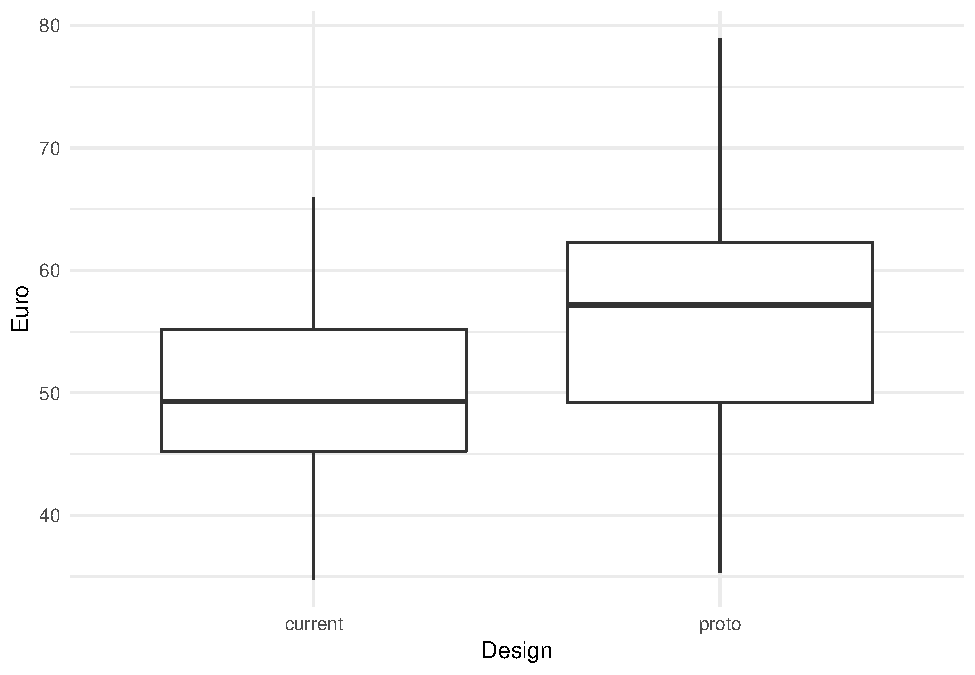
\includegraphics{Design_Research_files/figure-latex/rational_design_1-1.pdf}

There seems to be a slight benefit for the prototype condition. But, is
it a 10\% increase? And how certain can Violet be? A formal regression
analysis gives the answer \footnote{What we run here is a Gamma
  regression, which we will re-encounter in chapter {[}GLM{]}. The
  coefficients can directly be interpreted as changes in rate.}.

\begin{Shaded}
\begin{Highlighting}[]
\NormalTok{M_}\DecValTok{1}\NormalTok{ <-}\StringTok{ }
\StringTok{  }\NormalTok{RD }\OperatorTok\StringTok{ }
\StringTok{  }\KeywordTok{stan_glm}\NormalTok{(Euro }\OperatorTok{~}\StringTok{ }\NormalTok{Design, }
           \DataTypeTok{family =} \KeywordTok{Gamma}\NormalTok{(}\DataTypeTok{link=}\StringTok{"log"}\NormalTok{),}
      \DataTypeTok{data =}\NormalTok{ .)}

\NormalTok{P_}\DecValTok{1}\NormalTok{ <-}\StringTok{  }\KeywordTok{posterior}\NormalTok{(M_}\DecValTok{1}\NormalTok{)}
\end{Highlighting}
\end{Shaded}

\begin{Shaded}
\begin{Highlighting}[]
\NormalTok{T_fixef <-}\StringTok{ }\KeywordTok{fixef}\NormalTok{(P_}\DecValTok{1}\NormalTok{, }\DataTypeTok{mean.func =}\NormalTok{ exp)}
\NormalTok{T_fixef}
\end{Highlighting}
\end{Shaded}

\begin{longtable}[]{@{}lrrr@{}}
\toprule
fixef & center & lower & upper\tabularnewline
\midrule
\endhead
Intercept & 5.00e+01 & 4.70e+01 & 5.30e+01\tabularnewline
Designproto & 1.13e+00 & 1.03e+00 & 1.23e+00\tabularnewline
shape & 1.77e+09 & 8.00e+06 & 1.13e+12\tabularnewline
\bottomrule
\end{longtable}

The results tell her that participants spend \(49.975\) Euro on average
with the current design. The prototype seems to increase the revenue per
transaction by \(1.126\). That seems sufficient, but uncertainty is
strong, too, as indicated by the 95\% credibility intervals. There is a
chance of more than 2.5\%, that the revenue is just
\(47.035, 1.035, 8.003\times 10^{6}\) (or lower), such that the target
is not met. But what precisely is the chance of falling below EUR 5? In
Bayesian analysis we usually get the complete posterior distribution,
which we can evaluate to get a definite answer:

\emph{What is the probability of the increase in revenue being less than
5 EUR?}

We inspect the posterior distribution and mark the area of interest

\begin{Shaded}
\begin{Highlighting}[]
\NormalTok{N_risk_of_failure_}\DecValTok{1}\NormalTok{ <-}
\StringTok{  }\NormalTok{P_}\DecValTok{1} \OperatorTok
\StringTok{  }\KeywordTok{filter}\NormalTok{(parameter }\OperatorTok{==}\StringTok{ "Designproto"}\NormalTok{) }\OperatorTok
\StringTok{  }\KeywordTok{mutate}\NormalTok{(}\DataTypeTok{value =} \KeywordTok{exp}\NormalTok{(value),}
         \DataTypeTok{outcome =}\NormalTok{ value }\OperatorTok{<}\StringTok{ }\FloatTok{1.1}\NormalTok{) }\OperatorTok
\StringTok{  }\KeywordTok{select}\NormalTok{(outcome) }\OperatorTok
\StringTok{  }\NormalTok{colMeans  }

\NormalTok{P_}\DecValTok{1} \OperatorTok
\StringTok{  }\KeywordTok{filter}\NormalTok{(parameter }\OperatorTok{==}\StringTok{ "Designproto"}\NormalTok{) }\OperatorTok
\StringTok{  }\KeywordTok{mutate}\NormalTok{(}\DataTypeTok{value =} \KeywordTok{exp}\NormalTok{(value),}
         \DataTypeTok{outcome =} \KeywordTok{ifelse}\NormalTok{(value }\OperatorTok{<}\StringTok{ }\FloatTok{1.1}\NormalTok{, }\StringTok{"failure"}\NormalTok{, }\StringTok{"success"}\NormalTok{)) }\OperatorTok
\StringTok{  }\KeywordTok{ggplot}\NormalTok{(}\KeywordTok{aes}\NormalTok{(}\DataTypeTok{x =}\NormalTok{ value, }\DataTypeTok{fill =}\NormalTok{ outcome)) }\OperatorTok{+}
\StringTok{  }\KeywordTok{geom_histogram}\NormalTok{(}\DataTypeTok{binwidth =}\NormalTok{ .}\DecValTok{002}\NormalTok{)}
\end{Highlighting}
\end{Shaded}

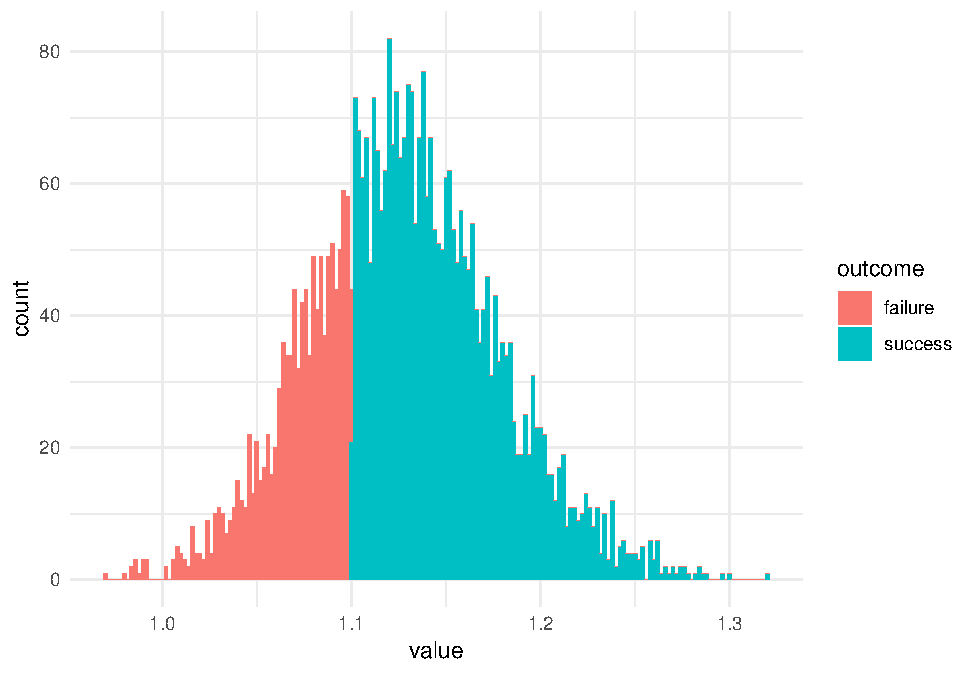
\includegraphics{Design_Research_files/figure-latex/rational_design_risk_of_failure-1.pdf}

\begin{Shaded}
\begin{Highlighting}[]
\KeywordTok{detach}\NormalTok{(Rational)  }
\end{Highlighting}
\end{Shaded}

The red area represents the danger zone, where revenue increase does not
reach EUR 5. The area amounts to 28.65\% of the total probability. With
this information the manager now has several options:

\begin{enumerate}
\def\labelenumi{\arabic{enumi})}
\tightlist
\item
  decides that 28.65\% is a risk she \emph{dares} to take
\item
  be confident in herself because \emph{past successes} prove that she
  should follow her intuition
\item
  take into account other \emph{sources of evidence}, for example expert
  opinions or meta studies
\item
  continue the study until sufficient evidence is gathered, but costs of
  additional effort have to be accounted for
\end{enumerate}

The first option represents an unspecific tolerance towards risk.
Extreme risk tolerance of managers is infamous as one cause for large
scale economic crises {[}BLACK\_SWANs{]}. Her motives could be manifold,
still: maybe she was nursed to take risks in her life; or she is
confident that consequences in case of failure will be bearable.

The second and third options have something in common: they make use of
\emph{external knowledge}. This is explained in the coming section. The
fourth option is another way of making \emph{cumulative use of
knowledge}, namely \emph{{[}adaptive testing: find correct term{]}}.

\subsection{Case: 99 seconds}\label{case99}

Consider Jane: she is chief engineer at a mega-large rent-a-car company
smartr.car that is doing their business nothing but online. Jane was
responsible for a large scale overhaul of the customer interface for
mobile users. Goal of the redesign was to streamline the user interface,
which had grown wild over the years and had become boring. Early
customer studies indicated that the app needed a serious visual
decluttering and stronger funneling of tasks. 300 person months went
into the re-development and the team did well: a recent A/B study had
shown that users learned the smartr.car v2.0 fast and could use its
functionality very efficiently. Jane's team is prepared for the
roll-out, when marketing requested the following:

\begin{quote}
marketing: we want to support market introduction with the following
slogan: ``rent a car in 99 seconds''.
\end{quote}

\begin{quote}
Jane: not all users manage a full transaction in that short time. That
could be a lie.
\end{quote}

\begin{quote}
marketing: legally, the claim is fine if it holds on average.
\end{quote}

\begin{quote}
Jane: i can find out for you (but we won't violate any rules).
\end{quote}

Jane takes another look at the performance of users in the smartr car
v2.0 condition. As she understands it, she has to find out whether the
average of all recorded time-on-tasks with smartr.car 2.0 is 99 seconds,
or better. Here is what she sees:

\begin{Shaded}
\begin{Highlighting}[]
\KeywordTok{attach}\NormalTok{(Sec99)}
\end{Highlighting}
\end{Shaded}

\begin{Shaded}
\begin{Highlighting}[]
\NormalTok{Ver20 }\OperatorTok\StringTok{   }
\StringTok{  }\KeywordTok{ggplot}\NormalTok{(}\KeywordTok{aes}\NormalTok{(}\DataTypeTok{x =}\NormalTok{ ToT)) }\OperatorTok{+}
\StringTok{  }\KeywordTok{geom_histogram}\NormalTok{()}
\end{Highlighting}
\end{Shaded}

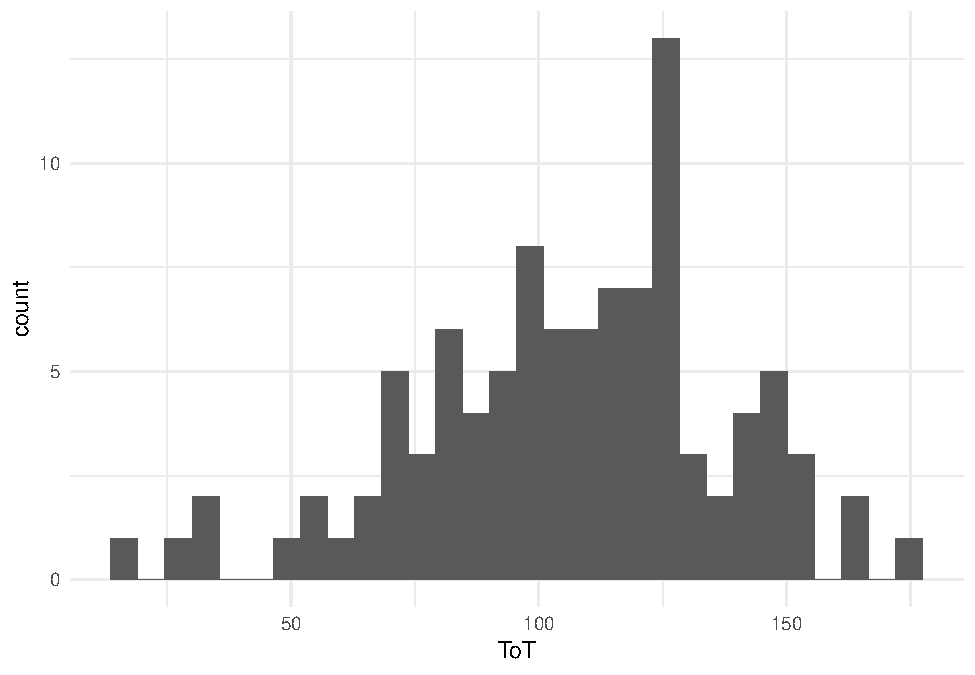
\includegraphics{Design_Research_files/figure-latex/seconds_99_1-1.pdf}

Jane, trained in statistics as she is, figures that if she would make
such a statement, she wanted to be 90\% sure. The performance is not
completely off 99 seconds. But given the huge variance in the sample, it
seems impossible to hold the desired claim with a certainty of 80\%.
Still, she gives it a try and runs an estimation (which we will later
get to know as a \emph{grand mean model})

\begin{Shaded}
\begin{Highlighting}[]
\NormalTok{M_}\DecValTok{1}\NormalTok{ <-}\StringTok{ }
\StringTok{  }\NormalTok{Ver20 }\OperatorTok\StringTok{    }
\StringTok{  }\KeywordTok{stan_glm}\NormalTok{(ToT }\OperatorTok{~}\StringTok{ }\DecValTok{1}\NormalTok{, }\DataTypeTok{data =}\NormalTok{ .)}

\NormalTok{P_}\DecValTok{1}\NormalTok{ <-}
\StringTok{  }\KeywordTok{posterior}\NormalTok{(M_}\DecValTok{1}\NormalTok{)}
\end{Highlighting}
\end{Shaded}

\begin{Shaded}
\begin{Highlighting}[]
\NormalTok{T_fixef <-}\StringTok{  }
\StringTok{  }\KeywordTok{fixef}\NormalTok{(P_}\DecValTok{1}\NormalTok{,}
        \DataTypeTok{interval =}\NormalTok{ .}\DecValTok{6}\NormalTok{)}

\NormalTok{N_99s <-}\StringTok{ }
\StringTok{  }\NormalTok{P_}\DecValTok{1} \OperatorTok\StringTok{ }
\StringTok{  }\KeywordTok{filter}\NormalTok{(parameter }\OperatorTok{==}\StringTok{ "Intercept"}\NormalTok{) }\OperatorTok\StringTok{ }
\StringTok{  }\KeywordTok{mutate}\NormalTok{(}\DataTypeTok{confirm =}\NormalTok{ value }\OperatorTok{<=}\StringTok{ }\DecValTok{99}\NormalTok{) }\OperatorTok\StringTok{ }
\StringTok{  }\KeywordTok{summarise}\NormalTok{(}\DataTypeTok{certainty =} \KeywordTok{mean}\NormalTok{(confirm)) }\OperatorTok\StringTok{ }
\StringTok{  }\KeywordTok{mutate}\NormalTok{(}\DataTypeTok{odds =}\NormalTok{ (}\DecValTok{1}\OperatorTok{-}\NormalTok{certainty)}\OperatorTok{/}\NormalTok{certainty) }\OperatorTok\StringTok{ }
\StringTok{  }\KeywordTok{as.numeric}\NormalTok{()}
  
\NormalTok{N_111s <-}\StringTok{ }
\StringTok{  }\NormalTok{P_}\DecValTok{1} \OperatorTok\StringTok{ }
\StringTok{  }\KeywordTok{filter}\NormalTok{(parameter }\OperatorTok{==}\StringTok{ "Intercept"}\NormalTok{) }\OperatorTok\StringTok{ }
\StringTok{  }\KeywordTok{mutate}\NormalTok{(}\DataTypeTok{confirm =}\NormalTok{ value }\OperatorTok{<=}\StringTok{ }\DecValTok{111}\NormalTok{) }\OperatorTok\StringTok{ }
\StringTok{  }\KeywordTok{summarise}\NormalTok{(}\DataTypeTok{certainty =} \KeywordTok{mean}\NormalTok{(confirm)) }\OperatorTok\StringTok{ }
\StringTok{  }\KeywordTok{mutate}\NormalTok{(}\DataTypeTok{odds =}\NormalTok{ (}\DecValTok{1}\OperatorTok{-}\NormalTok{certainty)}\OperatorTok{/}\NormalTok{certainty) }\OperatorTok\StringTok{ }
\StringTok{  }\KeywordTok{as.numeric}\NormalTok{()}
\end{Highlighting}
\end{Shaded}

\begin{Shaded}
\begin{Highlighting}[]
\KeywordTok{detach}\NormalTok{(Sec99)}
\end{Highlighting}
\end{Shaded}

The results tell her that most likely the average time-on-task is
\(fixef\). That is not very promising. In fact, the odds that the
average user can do it in 99 seconds is a feeble 2\%. Luckily, Jane had
the idea that the slogan could be changed to \emph{``rent a card in
1-1-1 seconds''}. The certainty that this slogan holds is a favorable
95, a risk that a brave marketing department is surely willing to take.

\subsection{Prior information}\label{prior-information}

It is rarely the case that we encounter a situation \emph{tabula rasa}.
Whether we are correct or not, when we look at the sky in the morning,
we have some expectations on how likely there will be rain. We also take
into account the season and the region. Even the planet is sometimes
taken into account: the Pathfinder probe carried a bag of gadgets, but
the umbrella was for safe landing only.

In behavioural research it has been general standard that every
experiment had to be judged on the produced data alone. For the sake of
objectivity, researchers were not allowed to take into account previous
results, let alone their personal opinion.

In Bayesian statistics, you have the choice. You can make use of
external knowledge, but you don't have to. In Bayesian terminology,
previous or external knowledge is called \emph{prior information}.
Kowledge that comes from the data is called the \emph{likelihood} and
both are combined to \emph{posterior} knowledge by multiplication:

\(posterior = likelihood * prior\)

Reconsider Violet, the rational e-commerce development manager. She had
this role for years and has supervised several large scale outrolls.
Couldn't she be more daring, taking into account her past successes?
This is not a completely new situation, after all.

The impact of prior information can range from negligible to
overwhelming. The gain in confidence in our example depends on three
factors:

\begin{enumerate}
\def\labelenumi{\arabic{enumi})}
\tightlist
\item
  the average magnitude of past successes, the higher, the better
\item
  the similarity of the current project with past projects
\item
  the amount of evidence (e.g., number of recorded projects)
\end{enumerate}

\begin{Shaded}
\begin{Highlighting}[]
\KeywordTok{attach}\NormalTok{(Rational)}
\end{Highlighting}
\end{Shaded}

\begin{Shaded}
\begin{Highlighting}[]
\NormalTok{M_prior <-}
\StringTok{  }\NormalTok{D_prior }\OperatorTok\StringTok{ }
\StringTok{  }\KeywordTok{stan_glm}\NormalTok{(revenue_increase }\OperatorTok{~}\StringTok{ }\DecValTok{1}\NormalTok{, }
           \DataTypeTok{family =} \KeywordTok{Gamma}\NormalTok{(}\DataTypeTok{link =} \StringTok{"log"}\NormalTok{),}
           \DataTypeTok{data =}\NormalTok{ .)}

\NormalTok{P_prior <-}\StringTok{ }\KeywordTok{posterior}\NormalTok{(M_prior)}
\end{Highlighting}
\end{Shaded}

Let's assume, the manager had done 5 projects in the past and recorded
the resulting change in revenues. On these five values she does a
regression, that we will later call an intercept-only model, and
concludes that her \emph{prior belief} is distributed as:

\begin{Shaded}
\begin{Highlighting}[]
\NormalTok{P_prior }\OperatorTok\StringTok{ }
\StringTok{  }\KeywordTok{filter}\NormalTok{(parameter }\OperatorTok{==}\StringTok{ "Intercept"}\NormalTok{) }\OperatorTok\StringTok{ }
\StringTok{  }\KeywordTok{mutate}\NormalTok{(}\DataTypeTok{value =} \KeywordTok{exp}\NormalTok{(value)) }\OperatorTok\StringTok{ }
\StringTok{  }\KeywordTok{ggplot}\NormalTok{(}\KeywordTok{aes}\NormalTok{(}\DataTypeTok{x =}\NormalTok{ value)) }\OperatorTok{+}
\StringTok{  }\KeywordTok{geom_density}\NormalTok{()}
\end{Highlighting}
\end{Shaded}

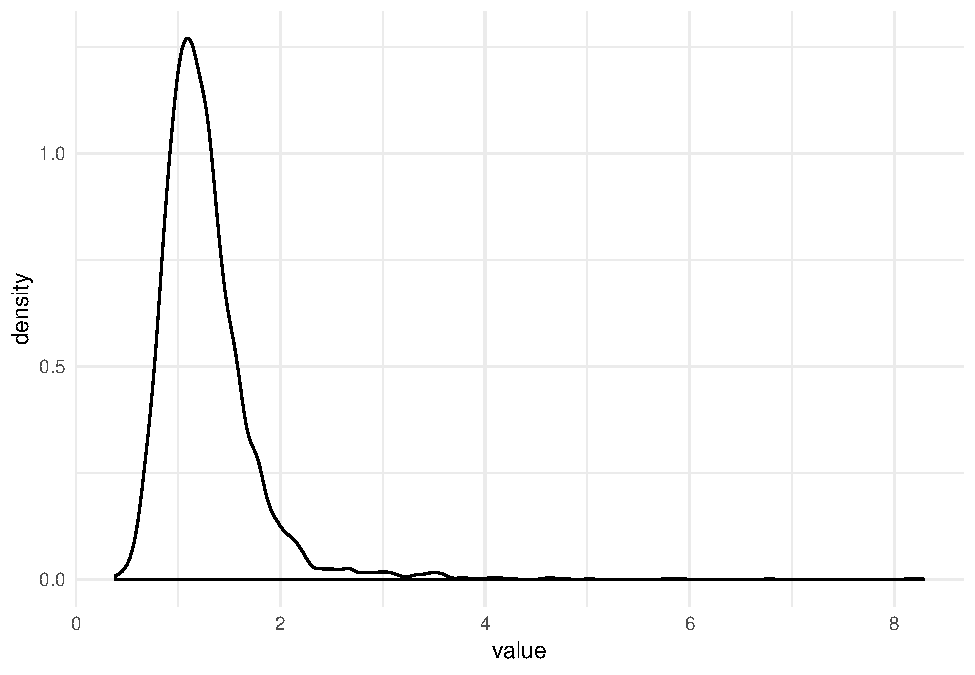
\includegraphics{Design_Research_files/figure-latex/previous_belief_in_revenue-1.pdf}

On average, revenues have increased by factor 1.211 by past design
improvements. Of course, with only five points of measurement there is
uncertainty as well. The mount of uncertainty is the spread of prior
distribution. Using this prior information, the development manager runs
another regression model on her experimental data, this time using both
sources of information, her optimistic prior and the experimental data.

\begin{Shaded}
\begin{Highlighting}[]
\NormalTok{M_}\DecValTok{2}\NormalTok{ <-}
\StringTok{  }\NormalTok{RD }\OperatorTok\StringTok{ }
\StringTok{  }\KeywordTok{stan_glm}\NormalTok{(Euro }\OperatorTok{~}\StringTok{ }\NormalTok{Design, }
      \DataTypeTok{prior_intercept =} \KeywordTok{normal}\NormalTok{(}\DecValTok{0}\NormalTok{, }\DecValTok{100}\NormalTok{),}
      \DataTypeTok{prior =} \KeywordTok{normal}\NormalTok{(T_prior[[}\DecValTok{1}\NormalTok{,}\DecValTok{2}\NormalTok{]], T_prior[[}\DecValTok{1}\NormalTok{,}\DecValTok{3}\NormalTok{]]),}
      \DataTypeTok{family =} \KeywordTok{Gamma}\NormalTok{(}\DataTypeTok{link =} \StringTok{"log"}\NormalTok{),}
      \DataTypeTok{data =}\NormalTok{ .)}

\NormalTok{P_}\DecValTok{2}\NormalTok{ <-}\StringTok{ }\KeywordTok{posterior}\NormalTok{(M_}\DecValTok{2}\NormalTok{)}
\end{Highlighting}
\end{Shaded}

\begin{Shaded}
\begin{Highlighting}[]
\NormalTok{T_fixef_}\DecValTok{2}\NormalTok{ <-}\StringTok{ }\KeywordTok{fixef}\NormalTok{(P_}\DecValTok{2}\NormalTok{, }\DataTypeTok{mean.func =}\NormalTok{ exp)}
\NormalTok{T_fixef_}\DecValTok{2}
\end{Highlighting}
\end{Shaded}

\begin{longtable}[]{@{}lrrr@{}}
\toprule
fixef & center & lower & upper\tabularnewline
\midrule
\endhead
Intercept & 4.99e+01 & 4.70e+01 & 5.31e+01\tabularnewline
Designproto & 1.13e+00 & 1.04e+00 & 1.23e+00\tabularnewline
shape & 1.66e+09 & 7.29e+06 & 1.13e+12\tabularnewline
\bottomrule
\end{longtable}

\begin{Shaded}
\begin{Highlighting}[]
\NormalTok{N_risk_of_failure_}\DecValTok{2}\NormalTok{ <-}
\StringTok{  }\NormalTok{P_}\DecValTok{2} \OperatorTok
\StringTok{  }\KeywordTok{filter}\NormalTok{(parameter }\OperatorTok{==}\StringTok{ "Designproto"}\NormalTok{) }\OperatorTok
\StringTok{  }\KeywordTok{mutate}\NormalTok{(}\DataTypeTok{value =} \KeywordTok{exp}\NormalTok{(value),}
         \DataTypeTok{outcome =}\NormalTok{ value }\OperatorTok{<}\StringTok{ }\FloatTok{1.1}\NormalTok{) }\OperatorTok
\StringTok{  }\KeywordTok{select}\NormalTok{(outcome) }\OperatorTok
\StringTok{  }\NormalTok{colMeans }

\NormalTok{  P_}\DecValTok{2} \OperatorTok
\StringTok{  }\KeywordTok{filter}\NormalTok{(parameter }\OperatorTok{==}\StringTok{ "Designproto"}\NormalTok{) }\OperatorTok
\StringTok{  }\KeywordTok{mutate}\NormalTok{(}\DataTypeTok{value =} \KeywordTok{exp}\NormalTok{(value),}
         \DataTypeTok{outcome =} \KeywordTok{ifelse}\NormalTok{(value }\OperatorTok{<}\StringTok{ }\FloatTok{1.1}\NormalTok{, }\StringTok{"failure"}\NormalTok{, }\StringTok{"success"}\NormalTok{)) }\OperatorTok
\StringTok{  }\KeywordTok{ggplot}\NormalTok{(}\KeywordTok{aes}\NormalTok{(}\DataTypeTok{x =}\NormalTok{ value, }\DataTypeTok{fill =}\NormalTok{ outcome)) }\OperatorTok{+}
\StringTok{  }\KeywordTok{geom_histogram}\NormalTok{(}\DataTypeTok{binwidth =}\NormalTok{ .}\DecValTok{002}\NormalTok{)}
\end{Highlighting}
\end{Shaded}

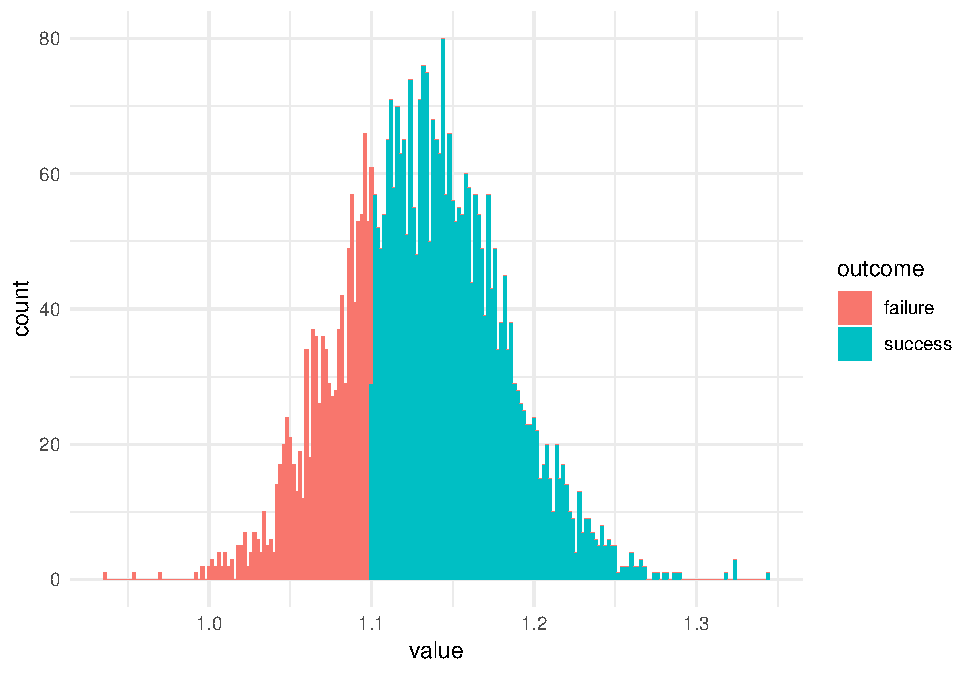
\includegraphics{Design_Research_files/figure-latex/rational_design_risk_of_failure_2-1.pdf}

\begin{Shaded}
\begin{Highlighting}[]
\KeywordTok{detach}\NormalTok{(Rational)}
\end{Highlighting}
\end{Shaded}

\chapter{Elements of Bayesian statistics}\label{bayesian_statistics}

As human beings we make our decisions on what has happened to us earlier
in time. For example, we trust a person or a company more, when we can
look back at a series of successful transactions. And we have remarkable
skills to recall what has just happened, but also what happened
yesterday or years ago. By integrating over all the evidence, we form a
view of the world we forage. When evidence is abundant, we believe
vigorously experience a feeling of certainty, or lack of doubt. That is
not to deny, that in a variety of situations, the boundedness of human
cognition kick in and we becaome terrible decision makers. This is for a
variety of psychological reasons, to name just a few:

\begin{itemize}
\tightlist
\item
  forgetting evidence
\item
  the primacy effect: recent events get more weight
\item
  confirmation bias: evidence that supports a belief is actively sought
  for, counter-evidence gets ignored.
\item
  the hindsight bias: once a situation has taken a certain outcome, we
  believe that it had to happen that way.
\end{itemize}

The very aim of scientific research is to avoid the pitfalls of our
minds and act as rational as possible by translating our theory into a
formal model, gathering evidence in an unbiased way and weigh the
evidence by formal procedures. When a statistic is reported together
with the strength of evidence, this is conventionally called an
\emph{inferential statistic}. In applied research, real world decisions
depend on the evidence, which has two aspects: first, the strength of
effects and the level of certainty we have reached.

Bayesian inferential statistics grounds on the idea of accumulating
evidence through and through. \emph{Certainty} (or belief or credibility
or credence) in Bayesian statistics is formalized as a \emph{probability
scale (0 = impossible, 1 = certain)}. Evidence accumulates by two
mechanisms, the successive observations in a data set and what has
already been learned in the past. When new data arrives and is analyzed,
a transition occurs from what you new before, \emph{prior belief}, to
what you know after seeing the data, \emph{posterior belief}. In other
words: by data the current belief gets an update.

In the following the essential concepts of statistics and Bayesian
analysis will be introduced.

\section{Descriptive statistics}\label{descriptive-statistics}

In empirical research we systematically gather observations.
Observations of the same kind are usually subsumed as variables. A set
of variables that have been gathered on the same sample are called a
data set, which typically is a table with variables in columns. In the
most general meaning, \emph{a statistic} is a single number that somehow
represents relevant features of a data set. Statistics fall into several
broad classes that answer certain types of questions:

\begin{itemize}
\tightlist
\item
  frequency: how many measures of a certain kind can be found in the
  data set?
\item
  central tendency: do measures tend to be located left (weak) or right
  (strong) on a scale?
\item
  dispersion: are measures close together or widely distributed along
  the scale?
\item
  association: does one variable X tend to change when another variable
  Y changes?
\end{itemize}

\subsection{Frequencies}\label{frequencies}

\begin{Shaded}
\begin{Highlighting}[]
\KeywordTok{attach}\NormalTok{(Sec99)}
\end{Highlighting}
\end{Shaded}

The most basic statistics of all probably is the number of observations
on a variable \(x\), usually denoted by \(n_{x}\). The number of
observations is a rough indicator for the amount of data that has been
gathered, which is directly linked to the level of certainty we can
reach.

\begin{Shaded}
\begin{Highlighting}[]
\KeywordTok{length}\NormalTok{(Ver20}\OperatorTok{$}\NormalTok{ToT)}
\end{Highlighting}
\end{Shaded}

\begin{verbatim}
## [1] 100
\end{verbatim}

The number of observations is not as trivial as it may appear at first.
In particular, it is usually not the same as the sample size, for two
reasons: First, most studies employ repeated measures to some extent.
You may have invited \(n_{Part}\) participants to your lab, but on each
participant you have obtained several measures of the same kind. When
every participant is tested on, let's say, five tasks, the amount of
data obtained gets larger. Second, taking a valid measure can always
fail for a variety of reasons, reasulting in \emph{missing values}. For
example, in the 99 seconds study, it has happened, that a few
participants missed to fill in their age on the intake form. The
researcher is left fewer measures of age \(n_{age}\) than there were
participants.

\begin{Shaded}
\begin{Highlighting}[]
\NormalTok{N <-}\StringTok{ }\ControlFlowTok{function}\NormalTok{(x) }\KeywordTok{sum}\NormalTok{(}\OperatorTok{!}\KeywordTok{is.na}\NormalTok{(x))}
\KeywordTok{N}\NormalTok{(Ver20}\OperatorTok{$}\NormalTok{age)}
\end{Highlighting}
\end{Shaded}

\begin{verbatim}
## [1] 97
\end{verbatim}

Another important issue is the distribution of measures across groups in
a data set. Again, the number of observations in a group is linked to
the certainty we can gain on that group. Furthermore, it is sometimes
important to have the distribution match the proportions in the
population, as otherwise biases may occur.

\begin{Shaded}
\begin{Highlighting}[]
\NormalTok{Ver20 }\OperatorTok\StringTok{ }
\StringTok{  }\KeywordTok{group_by}\NormalTok{(Gender) }\OperatorTok\StringTok{ }
\StringTok{  }\KeywordTok{summarize}\NormalTok{(}\KeywordTok{n}\NormalTok{())}
\end{Highlighting}
\end{Shaded}

\begin{tabular}{l|r}
\hline
Gender & n()\\
\hline
female & 59\\
\hline
male & 41\\
\hline
\end{tabular}

The table above shows so called absolute frequencies. When comparing
frequencies by groups, it often is more appropriate to report
\emph{relative frequencies} or \emph{proportions}:

\begin{Shaded}
\begin{Highlighting}[]
\NormalTok{n_Gender <-}\StringTok{ }\KeywordTok{N}\NormalTok{(Ver20}\OperatorTok{$}\NormalTok{Gender)}

\NormalTok{Ver20 }\OperatorTok
\StringTok{  }\KeywordTok{group_by}\NormalTok{(Gender) }\OperatorTok\StringTok{ }
\StringTok{  }\KeywordTok{summarize}\NormalTok{(}\DataTypeTok{proportion =} \KeywordTok{n}\NormalTok{()}\OperatorTok{/}\NormalTok{n_Gender)}
\end{Highlighting}
\end{Shaded}

\begin{tabular}{l|r}
\hline
Gender & proportion\\
\hline
female & 0.59\\
\hline
male & 0.41\\
\hline
\end{tabular}

Summarizing frequencies of metric measures, such as ToT or number of
errors is useful, too. However, a complication arises by the fact that
continuous measures do not naturally fall into groups. Especially in
duration measures no two measures are exactly the same.

\begin{Shaded}
\begin{Highlighting}[]
\KeywordTok{length}\NormalTok{(}\KeywordTok{unique}\NormalTok{(Ver20}\OperatorTok{$}\NormalTok{Gender))}
\end{Highlighting}
\end{Shaded}

\begin{verbatim}
## [1] 2
\end{verbatim}

\begin{Shaded}
\begin{Highlighting}[]
\KeywordTok{length}\NormalTok{(}\KeywordTok{unique}\NormalTok{(Ver20}\OperatorTok{$}\NormalTok{ToT))}
\end{Highlighting}
\end{Shaded}

\begin{verbatim}
## [1] 100
\end{verbatim}

The answer to this problem is \emph{binning}: the scale of measurement
is divided into a number of adjacent sections, called bins, and all
measures that fall into one bin are counted. For example, we could use
bins of 10 seconds and assess whether the bin with values larger than 90
and smaller or equal to 100 is representative in that it contains a
large proportion of values. As the histogram reveals, it is not very
representative.

\begin{Shaded}
\begin{Highlighting}[]
\NormalTok{bin <-}\StringTok{ }\ControlFlowTok{function}\NormalTok{(x, }\DataTypeTok{bin_width =} \DecValTok{10}\NormalTok{) }\KeywordTok{floor}\NormalTok{(x}\OperatorTok{/}\NormalTok{bin_width) }\OperatorTok{*}\StringTok{ }\NormalTok{bin_width}
\NormalTok{n_ToT <-}\StringTok{ }\KeywordTok{N}\NormalTok{(Ver20}\OperatorTok{$}\NormalTok{ToT)}

\NormalTok{Ver20 }\OperatorTok\StringTok{ }
\StringTok{  }\KeywordTok{mutate}\NormalTok{(}\DataTypeTok{bin =} \KeywordTok{bin}\NormalTok{(ToT)) }\OperatorTok\StringTok{ }
\StringTok{  }\KeywordTok{group_by}\NormalTok{(bin) }\OperatorTok\StringTok{ }
\StringTok{  }\KeywordTok{summarize}\NormalTok{(}\DataTypeTok{prop_ToT =} \KeywordTok{n}\NormalTok{()}\OperatorTok{/}\NormalTok{n_ToT) }\OperatorTok\StringTok{ }
\StringTok{  }\KeywordTok{ggplot}\NormalTok{(}\KeywordTok{aes}\NormalTok{(}\DataTypeTok{x =}\NormalTok{ bin, }\DataTypeTok{y =}\NormalTok{ prop_ToT)) }\OperatorTok{+}
\StringTok{  }\KeywordTok{geom_col}\NormalTok{()}
\end{Highlighting}
\end{Shaded}

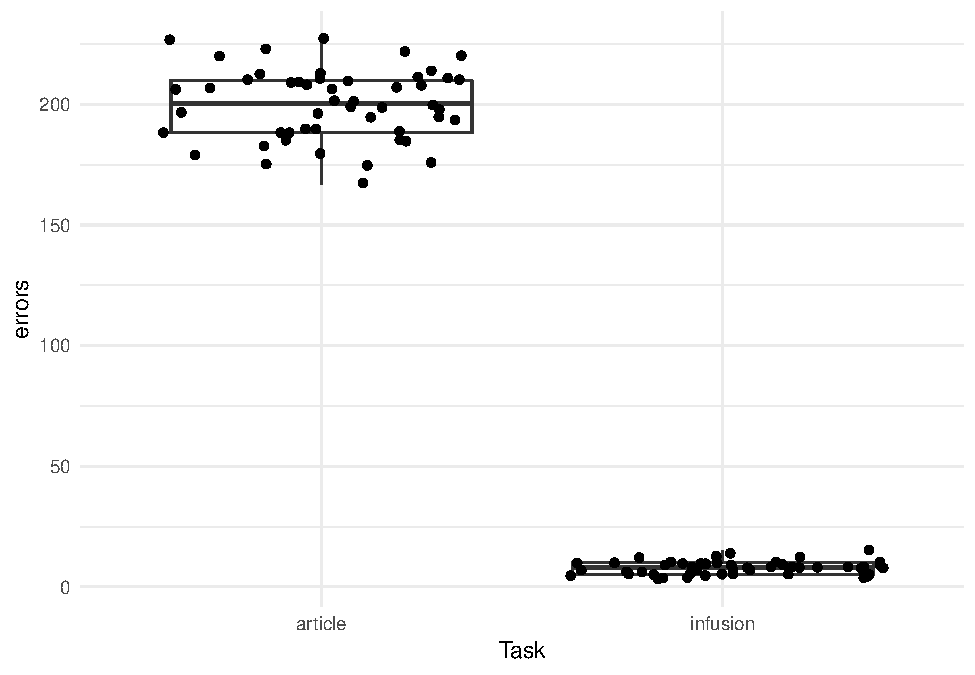
\includegraphics{Bayesian_statistics_files/figure-latex/unnamed-chunk-7-1.pdf}

\begin{Shaded}
\begin{Highlighting}[]
\CommentTok{# Ver20 %>% }
\CommentTok{#   ggplot(aes(x = ToT)) +}
\CommentTok{#   geom_histogram(binwidth = 10)}
\end{Highlighting}
\end{Shaded}

Strictly spoken, grouped and binned frequencies are not one statistic,
but a vector of statistics. A plot that shows the density of values in a
sequence of bins is called a histogram. It approximates what we will
later get to know more closely as a \emph{distribution}.

\subsection{Central tendency}\label{central-tendency}

Reconsider Jane \ref{case99}. When asked about whether users can
complete a transaction within 99, she looked at the population average
of her measures. The population average is what we call the
\emph{(arithmetic) mean}. The mean is computed by summing over all
measures and divide by the number of observations.

\begin{Shaded}
\begin{Highlighting}[]
\NormalTok{mean <-}\StringTok{ }\ControlFlowTok{function}\NormalTok{(x) }\KeywordTok{sum}\NormalTok{(x)}\OperatorTok{/}\KeywordTok{length}\NormalTok{(x)}
\end{Highlighting}
\end{Shaded}

\begin{Shaded}
\begin{Highlighting}[]
\KeywordTok{mean}\NormalTok{(Ver20}\OperatorTok{$}\NormalTok{ToT)}
\end{Highlighting}
\end{Shaded}

\begin{verbatim}
## [1] 106
\end{verbatim}

Imagine a competitor would go to court. Not an expert in that matter, my
humble opinion is that one of the first questions to be regarded
probably is: what does ``rent a car in 99 seconds'' actually promise?
And here are some other ways to interpret the same slogan:

``\emph{50\% (or more) of users} can rent a car in 99 seconds''. This is
called the \emph{median}. The median is computed by bringing all
measures into an order and collect the element right in the center, or
the mean of the center pair of values when the number of observations is
even.

The median is a special case of so called \emph{quantiles}. The court
could decide that 50\% of users is too lenient as a criterion and could
demand that 75\% percent of users must complete the task within 99
seconds for the slogan to be considered valid.

\begin{Shaded}
\begin{Highlighting}[]
\KeywordTok{quantile}\NormalTok{(Ver20}\OperatorTok{$}\NormalTok{ToT, .}\DecValTok{75}\NormalTok{)}
\end{Highlighting}
\end{Shaded}

\begin{verbatim}
## 75% 
## 125
\end{verbatim}

A common pattern in the distribution of measures is that a majority of
observations densely accumulate in the center region. The point of
highest density of a distribution is called the \emph{mode}. In other
words: the mode is the region (or point) that is most likely to occur.
For continuous measures this once again poses the problem that every
value is unique. Sophisticated procedures exist to smooth over this
inconvenience, but by binning we can construct an approximation of the
mode: just choose the center of the bin with highest frequency.

\begin{Shaded}
\begin{Highlighting}[]
\NormalTok{median <-}\StringTok{ }\ControlFlowTok{function}\NormalTok{(x)\{ }
\NormalTok{  n <-}\StringTok{ }\KeywordTok{length}\NormalTok{(x)}
\NormalTok{  center <-}\StringTok{ }\NormalTok{(n }\OperatorTok{+}\StringTok{ }\DecValTok{1}\NormalTok{)}\OperatorTok\DecValTok{2}
    \ControlFlowTok{if}\NormalTok{ (n}\OperatorTok\DecValTok{2} \OperatorTok{==}\StringTok{ }\DecValTok{1}\NormalTok{) }
        \KeywordTok{sort}\NormalTok{(x, }\DataTypeTok{partial =}\NormalTok{ half)[half]}
    \ControlFlowTok{else} \KeywordTok{mean}\NormalTok{(}\KeywordTok{sort}\NormalTok{(x, }\DataTypeTok{partial =}\NormalTok{ half }\OperatorTok{+}\StringTok{ }\DecValTok{0}\OperatorTok{:}\DecValTok{1}\NormalTok{)[half }\OperatorTok{+}\StringTok{ }\DecValTok{0}\OperatorTok{:}\DecValTok{1}\NormalTok{])}
\NormalTok{\}}
\end{Highlighting}
\end{Shaded}

\begin{Shaded}
\begin{Highlighting}[]
\NormalTok{mode <-}\StringTok{ }\ControlFlowTok{function}\NormalTok{(x, }\DataTypeTok{bin_width =} \DecValTok{10}\NormalTok{) \{}
\NormalTok{  bins <-}\StringTok{ }\KeywordTok{bin}\NormalTok{(x, bin_width)}
\NormalTok{  bins[}\KeywordTok{which.max}\NormalTok{(}\KeywordTok{tabulate}\NormalTok{(}\KeywordTok{match}\NormalTok{(x, bins)))] }\OperatorTok{+}\StringTok{ }\NormalTok{bin_width}\OperatorTok{/}\DecValTok{2}
\NormalTok{\}}
\end{Highlighting}
\end{Shaded}

\begin{Shaded}
\begin{Highlighting}[]
\NormalTok{knit_print.tbl_obs <-}\StringTok{ }\ControlFlowTok{function}\NormalTok{(x, ...) \{}
  \CommentTok{#data_set <- deparse(substitute(x))}
\NormalTok{  n <-}\StringTok{ }\KeywordTok{min}\NormalTok{(}\DecValTok{8}\NormalTok{, }\KeywordTok{nrow}\NormalTok{(x))}
\NormalTok{  tab <-}\StringTok{ }\NormalTok{dplyr}\OperatorTok{::}\KeywordTok{sample_n}\NormalTok{(x, n)}
  \ControlFlowTok{if}\NormalTok{(}\StringTok{"Obs"} \OperatorTok\StringTok{ }\KeywordTok{colnames}\NormalTok{(tab)) tab <-}\StringTok{ }\NormalTok{dplyr}\OperatorTok{::}\KeywordTok{arrange}\NormalTok{(tab, Obs)}
  \ControlFlowTok{if}\NormalTok{(}\StringTok{"Part"} \OperatorTok\StringTok{ }\KeywordTok{colnames}\NormalTok{(tab)) tab <-}\StringTok{ }\NormalTok{dplyr}\OperatorTok{::}\KeywordTok{arrange}\NormalTok{(tab, Part)}
\NormalTok{  cap <-}\StringTok{ }\NormalTok{stringr}\OperatorTok{::}\KeywordTok{str_c}\NormalTok{(}\StringTok{"Data set"}\NormalTok{,}\StringTok{": showing "}\NormalTok{, n, }\StringTok{" of "}\NormalTok{, }\KeywordTok{nrow}\NormalTok{(x), }\StringTok{" observations"}\NormalTok{)}

\NormalTok{  res =}\StringTok{ }\KeywordTok{paste}\NormalTok{(}\KeywordTok{c}\NormalTok{(}\StringTok{""}\NormalTok{, }\StringTok{""}\NormalTok{, knitr}\OperatorTok{::}\KeywordTok{kable}\NormalTok{(tab, }\DataTypeTok{caption =}\NormalTok{ cap, }\DataTypeTok{format =} \StringTok{"markdown"}\NormalTok{, ...)),}
              \DataTypeTok{collapse =} \StringTok{"}\CharTok{\textbackslash{}n}\StringTok{"}\NormalTok{)}
\NormalTok{  knitr}\OperatorTok{::}\KeywordTok{asis_output}\NormalTok{(res)}
\NormalTok{\}}
\end{Highlighting}
\end{Shaded}

\begin{Shaded}
\begin{Highlighting}[]
\NormalTok{Ver20}
\end{Highlighting}
\end{Shaded}

\begin{longtable}[]{@{}rrrrl@{}}
\toprule
Obs & Part & ToT & age & Gender\tabularnewline
\midrule
\endhead
21 & 21 & 95.8 & 44 & male\tabularnewline
34 & 34 & 86.7 & 42 & female\tabularnewline
36 & 36 & 53.5 & 29 & male\tabularnewline
38 & 38 & 79.5 & 36 & male\tabularnewline
40 & 40 & 106.1 & 36 & female\tabularnewline
59 & 59 & 15.2 & 27 & male\tabularnewline
83 & 83 & 107.7 & 47 & female\tabularnewline
90 & 90 & 129.7 & 42 & male\tabularnewline
\bottomrule
\end{longtable}

\begin{Shaded}
\begin{Highlighting}[]
\NormalTok{Ver20 }\OperatorTok\StringTok{ }
\StringTok{  }\KeywordTok{group_by}\NormalTok{() }\OperatorTok\StringTok{ }
\StringTok{  }\KeywordTok{summarize}\NormalTok{(}
    \DataTypeTok{mean_ToT   =} \KeywordTok{mean}\NormalTok{(ToT),}
    \DataTypeTok{median_ToT =} \KeywordTok{median}\NormalTok{(ToT),}
    \DataTypeTok{mode_ToT =} \KeywordTok{mode}\NormalTok{(ToT)) }\OperatorTok\StringTok{ }
\StringTok{  }\KeywordTok{knit_print.tbl_obs}\NormalTok{()}
\end{Highlighting}
\end{Shaded}

\begin{longtable}[]{@{}rrr@{}}
\toprule
mean\_ToT & median\_ToT & mode\_ToT\tabularnewline
\midrule
\endhead
106 & 108 & 145\tabularnewline
\bottomrule
\end{longtable}

The table above shows the three statistics for central tendency
side-by-side. Mean and median are close together. This is frequently the
case, but not always. When the distribution of measures is completely
symmetric mean and median perfectly coincide. In section
@\ref(distributions) we will encounter distributions that are not
symmetric. The more a distribution is skewed, the stronger the
difference between mean and median increases.

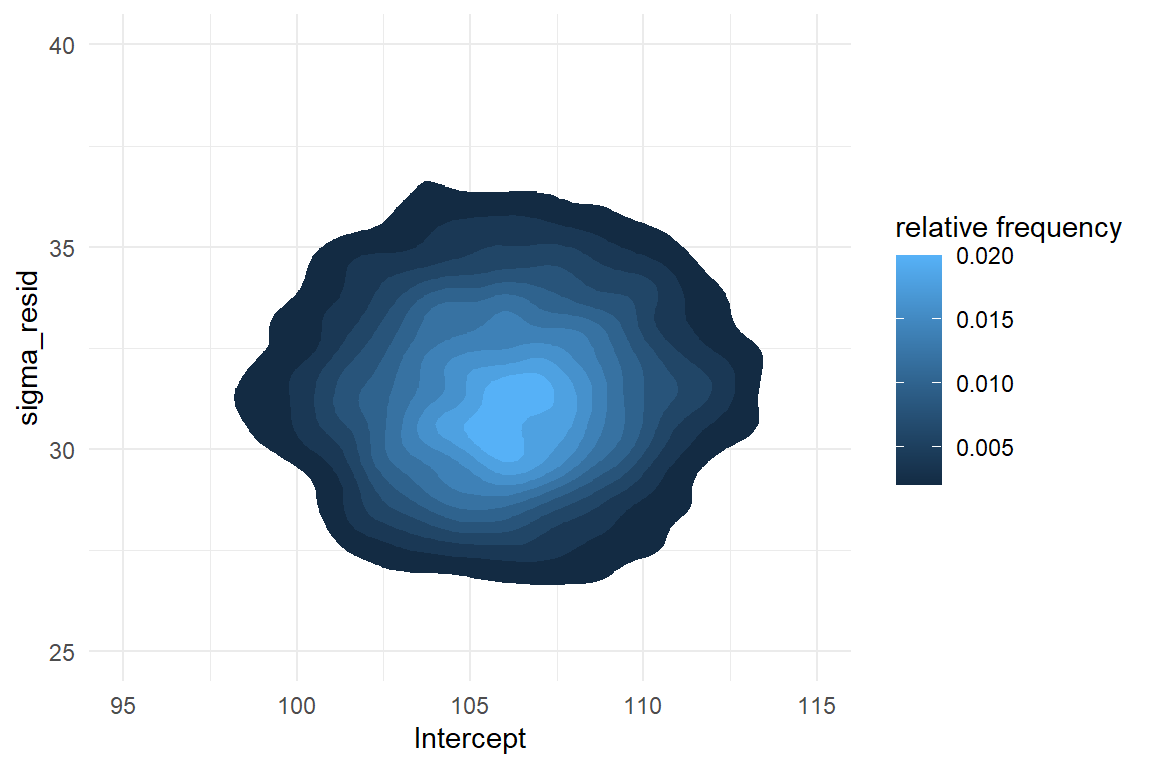
\includegraphics{Bayesian_statistics_files/figure-latex/unnamed-chunk-16-1.pdf}

To be more precise: for left skewed distributions the mean is strongly
influenced by few, but extreme, values in the left tail of the
distribution. The median only counts the number of observations to both
sides and is not influenced by how extreme these values are. Therefore,
it is located more to the right. The mode does not regard any values
other than those in the densest region and just marks that peak. The
same principles hold for right-skewed distributions.

To summarize, the mean is the most frequently used measure of central
tendency, one reason being that it is a so called \emph{sufficient
statistic}, meaning that it exploits the full information present in the
data. The median is frequently used when extreme measures are a concern.
The mode is the point in the distribution that is most typical.

\subsection{Dispersion}\label{dispersion}

In a symmetric distribution with exactly one peak, mean and mode
coincide and the mean represents the most typical value. For a value
being more typical does not mean it is very typical. That depends on how
the measures are dispersed over the whole range. In the figure below,
the center value of the narrow distribution contains 60\% of all
measures, as compared to 40\% in the wide distribution, and is therefore
more representative.

\begin{Shaded}
\begin{Highlighting}[]
\NormalTok{D_disp <-}
\StringTok{  }\KeywordTok{tribble}\NormalTok{(}\OperatorTok{~}\NormalTok{y, }\OperatorTok{~}\NormalTok{narrow, }\OperatorTok{~}\NormalTok{wide,}
        \DecValTok{1}\NormalTok{, }\DecValTok{0}\NormalTok{, }\DecValTok{1}\NormalTok{,}
        \DecValTok{2}\NormalTok{, }\DecValTok{2}\NormalTok{, }\DecValTok{2}\NormalTok{,}
        \DecValTok{3}\NormalTok{, }\DecValTok{6}\NormalTok{, }\DecValTok{4}\NormalTok{,}
        \DecValTok{4}\NormalTok{, }\DecValTok{2}\NormalTok{, }\DecValTok{2}\NormalTok{,}
        \DecValTok{5}\NormalTok{, }\DecValTok{0}\NormalTok{, }\DecValTok{1}\NormalTok{) }\OperatorTok\StringTok{ }
\StringTok{  }\KeywordTok{gather}\NormalTok{(Distribution, frequency, }\OperatorTok{-}\NormalTok{y) }


\NormalTok{D_disp }\OperatorTok\StringTok{ }
\StringTok{  }\KeywordTok{ggplot}\NormalTok{(}\KeywordTok{aes}\NormalTok{(}\DataTypeTok{x =}\NormalTok{ y, }
             \DataTypeTok{y =}\NormalTok{ frequency)) }\OperatorTok{+}
\StringTok{  }\KeywordTok{facet_grid}\NormalTok{(Distribution }\OperatorTok{~}\StringTok{ }\NormalTok{.) }\OperatorTok{+}
\StringTok{  }\KeywordTok{geom_col}\NormalTok{()}
\end{Highlighting}
\end{Shaded}

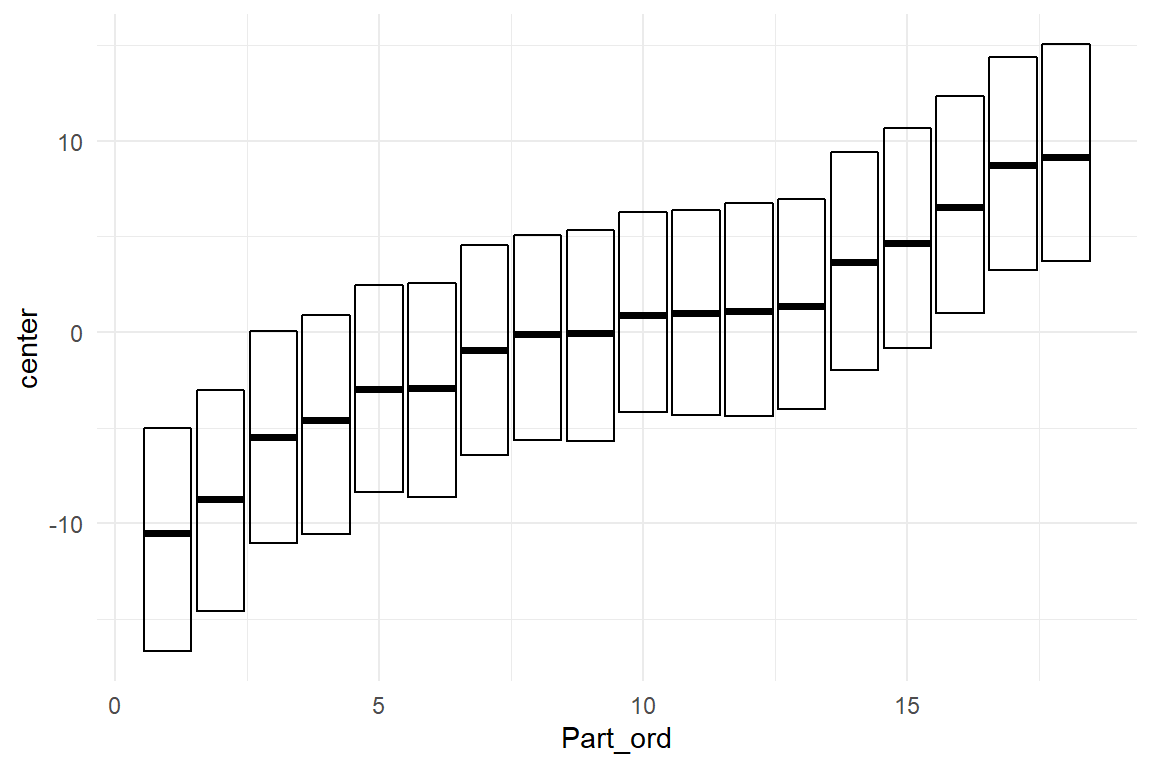
\includegraphics{Bayesian_statistics_files/figure-latex/unnamed-chunk-17-1.pdf}

A very basic way to describe dispersion of a distribution is to report
the \emph{range} between the two extreme values, \emph{minimum} and
\emph{maximum}. These are easily computed by sorting all values and
selecting the first and the last element. Coincidentally, they are also
special cases of quantiles, namely the 0\% and 100\% quantiles.

The range statistic only uses just these two values and therefore does
not fully represent the amount of dispersion. A statistic for dispersion
that does so is the \emph{variance}, which is the mean of squared
deviatons from the mean. Squaring the deviations always produces a
positive value, but makes variance difficult to interpret. The
\emph{standard deviation} is the square root of variance. By reversing
the square the standard deviation is on the same scale as the original
measures and their mean.

\begin{Shaded}
\begin{Highlighting}[]
\NormalTok{min <-}\StringTok{ }\ControlFlowTok{function}\NormalTok{(x) }\KeywordTok{sort}\NormalTok{(x)[}\DecValTok{1}\NormalTok{]}
\NormalTok{max <-}\StringTok{ }\ControlFlowTok{function}\NormalTok{(x) }\KeywordTok{quantile}\NormalTok{(x, }\DecValTok{1}\NormalTok{)}
\NormalTok{range <-}\StringTok{ }\ControlFlowTok{function}\NormalTok{(x) }\KeywordTok{max}\NormalTok{(x) }\OperatorTok{-}\StringTok{ }\KeywordTok{min}\NormalTok{(x)}
\NormalTok{var <-}\StringTok{ }\ControlFlowTok{function}\NormalTok{(x) }\KeywordTok{mean}\NormalTok{((}\KeywordTok{mean}\NormalTok{(x) }\OperatorTok{-}\StringTok{ }\NormalTok{x)}\OperatorTok{^}\DecValTok{2}\NormalTok{)}
\NormalTok{sd  <-}\StringTok{ }\ControlFlowTok{function}\NormalTok{(x) }\KeywordTok{sqrt}\NormalTok{(}\KeywordTok{var}\NormalTok{(x))}

\NormalTok{Ver20 }\OperatorTok\StringTok{ }
\StringTok{  }\KeywordTok{summarize}\NormalTok{(}\KeywordTok{min}\NormalTok{(ToT),}
            \KeywordTok{max}\NormalTok{(ToT),}
            \KeywordTok{range}\NormalTok{(ToT),}
            \KeywordTok{var}\NormalTok{(ToT),}
            \KeywordTok{sd}\NormalTok{(ToT))}
\end{Highlighting}
\end{Shaded}

\begin{longtable}[]{@{}rrrrr@{}}
\toprule
min(ToT) & max(ToT) & range(ToT) & var(ToT) & sd(ToT)\tabularnewline
\midrule
\endhead
15.2 & 174 & 158 & 966 & 31.1\tabularnewline
\bottomrule
\end{longtable}

\begin{Shaded}
\begin{Highlighting}[]
\KeywordTok{detach}\NormalTok{(Sec99)}
\end{Highlighting}
\end{Shaded}

\subsection{Associations}\label{associations}

Are elderly users slower at navigating websites? How does reading speed
depend on font size? Is the result of an intelligence test independent
from gender?

A majority of research deals with associations between variables and the
present section introduces some statistics to describe them. Variables
represent properties of the objects of research and fall into two
categories: \emph{Metric variables} represent a measured property, such
as speed, height, money or perceived satisfaction. \emph{Categorial
variables} put observations (or objects of research) into
non-overlapping groups, such as experimental conditions, persons who can
program or cannot, type of education etc. Consequently, associations
between any two variables fall into precisely one of three cases:

\begin{longtable}[]{@{}lll@{}}
\toprule
& categorial & metric\tabularnewline
\midrule
\endhead
categorial & frequency cross tables & differences in mean\tabularnewline
- & - & -\tabularnewline
metric & & covariance, correlation\tabularnewline
- & - & -\tabularnewline
\bottomrule
\end{longtable}

All forms of associations derive directly from statistics we have
already encountered. That is obvious for when one variable is categorial
and a little more subtle for two metric variables.

When there are only categories in the game, but no measures, the only
way to compare is by frequencies. To illustrate the
categorial-categorial case, consider a study to assess the safety of two
syringe infusion pump designs, called Legacy and Novel. All participants
of the study are asked to perform a typical sequence of operation and it
is recorded whether the sequence was completed correctly or not.

\begin{Shaded}
\begin{Highlighting}[]
\KeywordTok{attach}\NormalTok{(IPump)}

\NormalTok{D_agg }\OperatorTok\StringTok{ }
\StringTok{  }\KeywordTok{filter}\NormalTok{(Session }\OperatorTok{==}\StringTok{ }\DecValTok{3}\NormalTok{) }\OperatorTok\StringTok{ }
\StringTok{  }\KeywordTok{group_by}\NormalTok{(Design, completion) }\OperatorTok\StringTok{ }
\StringTok{  }\KeywordTok{summarize}\NormalTok{(}\DataTypeTok{frequency =} \KeywordTok{n}\NormalTok{()) }\OperatorTok
\StringTok{  }\KeywordTok{ungroup}\NormalTok{() }\OperatorTok\StringTok{ }
\StringTok{  }\KeywordTok{spread}\NormalTok{(completion, frequency)}
\end{Highlighting}
\end{Shaded}

\begin{tabular}{l|r|r}
\hline
Design & FALSE & TRUE\\
\hline
Legacy & 21 & 4\\
\hline
Novel & 22 & 3\\
\hline
\end{tabular}

Besides the troubling result that incorrect completion is the rule, not
the exception, there is almost no difference between the two designs.
Note that in this study, both professional groups were even in number.
If that is not the case, it is preferred to report proportions within a
group. Note how every row sums up to \(1\).

\begin{Shaded}
\begin{Highlighting}[]
\NormalTok{D_agg }\OperatorTok\StringTok{ }
\StringTok{  }\KeywordTok{filter}\NormalTok{(Session }\OperatorTok{==}\StringTok{ }\DecValTok{3}\NormalTok{) }\OperatorTok\StringTok{ }
\StringTok{  }\KeywordTok{group_by}\NormalTok{(Design, completion) }\OperatorTok\StringTok{ }
\StringTok{  }\KeywordTok{summarize}\NormalTok{(}\DataTypeTok{frequency =} \KeywordTok{n}\NormalTok{()) }\OperatorTok\StringTok{ }
\StringTok{  }\KeywordTok{group_by}\NormalTok{(Design) }\OperatorTok
\StringTok{  }\KeywordTok{mutate}\NormalTok{(}\DataTypeTok{frequency =}\NormalTok{ frequency}\OperatorTok{/}\KeywordTok{sum}\NormalTok{(frequency)) }\OperatorTok\StringTok{ }
\StringTok{  }\KeywordTok{ungroup}\NormalTok{() }\OperatorTok\StringTok{ }
\StringTok{  }\KeywordTok{spread}\NormalTok{(completion, frequency)}
\end{Highlighting}
\end{Shaded}

\begin{tabular}{l|r|r}
\hline
Design & FALSE & TRUE\\
\hline
Legacy & 0.84 & 0.16\\
\hline
Novel & 0.88 & 0.12\\
\hline
\end{tabular}

In a similar manner, associations between groups and metric variables
are reported by group means. In the case of the two infusion pump
designs, the time spent to complete the sequence is compared by the
following table. And as you can see, adding a comparison of variance is
no hassle.

\begin{Shaded}
\begin{Highlighting}[]
\NormalTok{D_agg }\OperatorTok\StringTok{ }
\StringTok{  }\KeywordTok{filter}\NormalTok{(Session }\OperatorTok{==}\StringTok{ }\DecValTok{3}\NormalTok{) }\OperatorTok\StringTok{ }
\StringTok{  }\KeywordTok{group_by}\NormalTok{(Design) }\OperatorTok\StringTok{ }
\StringTok{  }\KeywordTok{summarize}\NormalTok{(}\DataTypeTok{mean_ToT =} \KeywordTok{mean}\NormalTok{(ToT),}
            \DataTypeTok{sd_ToT =} \KeywordTok{sd}\NormalTok{(ToT))}
\end{Highlighting}
\end{Shaded}

\begin{tabular}{l|r|r}
\hline
Design & mean\_ToT & sd\_ToT\\
\hline
Legacy & 151.0 & 62.2\\
\hline
Novel & 87.7 & 33.8\\
\hline
\end{tabular}

For associations between two metric variables, \emph{covariance} is a
commonly employed statistic for the association between two variables
and derives directly from variance, with the difference that the square
of deviations is replaced by the multiplication of two deviations. For
example, we may want to assess whether there is any relationship between
years of experience and ToT:

\[
\textrm{cov}_{XY} = \frac{1}{n} \sum_{i=1}^n (x_i - E(X)) (y_i - E(Y))
\]

\begin{Shaded}
\begin{Highlighting}[]
\NormalTok{cov <-}\StringTok{ }\ControlFlowTok{function}\NormalTok{(x, y)}
  \KeywordTok{mean}\NormalTok{((x }\OperatorTok{-}\StringTok{ }\KeywordTok{mean}\NormalTok{(x, }\DataTypeTok{na.rm =}\NormalTok{ T)) }\OperatorTok{*}\StringTok{ }\NormalTok{(y }\OperatorTok{-}\StringTok{ }\KeywordTok{mean}\NormalTok{(y, }\DataTypeTok{na.rm =}\NormalTok{ T)), }\DataTypeTok{na.rm =}\NormalTok{ T)}
\end{Highlighting}
\end{Shaded}

\begin{Shaded}
\begin{Highlighting}[]
\KeywordTok{cov}\NormalTok{(D_agg}\OperatorTok{$}\NormalTok{experience, D_agg}\OperatorTok{$}\NormalTok{ToT)}
\end{Highlighting}
\end{Shaded}

\begin{verbatim}
## [1] 271
\end{verbatim}

When at large the deviations go into the same direction from the
respective mean, covariance becomes positive. When the deviations
primarily move in opposite direction it is negative. When the picture is
mixed, covariance will stay close to zero. The three plots below
illustrate three covariances, a strongly positive, a weakly positive and
a moderate negative one.

\begin{Shaded}
\begin{Highlighting}[]
\NormalTok{cor2cov <-}\StringTok{ }\ControlFlowTok{function}\NormalTok{(cor, sd) }\KeywordTok{diag}\NormalTok{(sd) }\OperatorTok\StringTok{ }\NormalTok{cor }\OperatorTok\StringTok{ }\KeywordTok{t}\NormalTok{(}\KeywordTok{diag}\NormalTok{(sd))}

\NormalTok{cor_mat <-}\StringTok{ }\KeywordTok{matrix}\NormalTok{(}\KeywordTok{c}\NormalTok{(}\DecValTok{1}\NormalTok{, .}\DecValTok{95}\NormalTok{, }\OperatorTok{-}\NormalTok{.}\DecValTok{5}\NormalTok{, .}\DecValTok{2}\NormalTok{, }
\NormalTok{                    .}\DecValTok{95}\NormalTok{, }\DecValTok{1}\NormalTok{, }\OperatorTok{-}\NormalTok{.}\DecValTok{5}\NormalTok{, .}\DecValTok{2}\NormalTok{,}
                    \OperatorTok{-}\NormalTok{.}\DecValTok{5}\NormalTok{, }\OperatorTok{-}\NormalTok{.}\DecValTok{5}\NormalTok{,  }\DecValTok{1}\NormalTok{, .}\DecValTok{15}\NormalTok{, }
\NormalTok{                    .}\DecValTok{2}\NormalTok{, .}\DecValTok{2}\NormalTok{, .}\DecValTok{15}\NormalTok{, }\DecValTok{1}\NormalTok{), }\DataTypeTok{ncol =} \DecValTok{4}\NormalTok{)}
\NormalTok{sd_vec  <-}\StringTok{ }\KeywordTok{c}\NormalTok{(.}\DecValTok{2}\NormalTok{, .}\DecValTok{2}\NormalTok{, }\DecValTok{40}\NormalTok{, }\DecValTok{2}\NormalTok{)}
\NormalTok{mean_vec <-}\StringTok{ }\KeywordTok{c}\NormalTok{(}\DecValTok{2}\NormalTok{, }\DecValTok{2}\NormalTok{, }\DecValTok{180}\NormalTok{, }\DecValTok{6}\NormalTok{)}

\NormalTok{D_psychomet <-}\StringTok{ }
\StringTok{  }\NormalTok{mvtnorm}\OperatorTok{::}\KeywordTok{rmvnorm}\NormalTok{(}\DecValTok{300}\NormalTok{, }\DataTypeTok{mean =}\NormalTok{ mean_vec, }\DataTypeTok{sigma =} \KeywordTok{cor2cov}\NormalTok{(cor_mat, sd_vec)) }\OperatorTok
\StringTok{  }\KeywordTok{as.tibble}\NormalTok{() }\OperatorTok\StringTok{ }
\StringTok{  }\KeywordTok{rename}\NormalTok{(}\DataTypeTok{MRS_1 =}\NormalTok{ V1, }\DataTypeTok{MRS_2 =}\NormalTok{ V2, }\DataTypeTok{ToT =}\NormalTok{ V3, }\DataTypeTok{VSWM =}\NormalTok{ V4)}
\end{Highlighting}
\end{Shaded}

\begin{Shaded}
\begin{Highlighting}[]
\NormalTok{deviation <-}\StringTok{ }\ControlFlowTok{function}\NormalTok{(x) }\KeywordTok{mean}\NormalTok{(x) }\OperatorTok{-}\NormalTok{x}
\NormalTok{direction <-}\StringTok{ }\ControlFlowTok{function}\NormalTok{(x,y) }\KeywordTok{if_else}\NormalTok{(}\KeywordTok{sign}\NormalTok{(}\KeywordTok{deviation}\NormalTok{(x)) }\OperatorTok{==}\StringTok{ }\KeywordTok{sign}\NormalTok{(}\KeywordTok{deviation}\NormalTok{(y)), }\StringTok{"same"}\NormalTok{, }\StringTok{"opposite"}\NormalTok{)}
\NormalTok{ggcov     <-}\StringTok{ }\ControlFlowTok{function}\NormalTok{(D, x, y, }\DataTypeTok{legend.position =} \StringTok{"none"}\NormalTok{)   \{}
\NormalTok{  quo_x <-}\StringTok{ }\KeywordTok{enquo}\NormalTok{(x)}
\NormalTok{  quo_y <-}\StringTok{ }\KeywordTok{enquo}\NormalTok{(y)}
\NormalTok{  out <-}\StringTok{ }
\StringTok{    }\NormalTok{D }\OperatorTok\StringTok{ }
\StringTok{    }\KeywordTok{mutate}\NormalTok{(}\DataTypeTok{Direction =} \KeywordTok{direction}\NormalTok{(}\OperatorTok{!!}\StringTok{ }\NormalTok{quo_x, }\OperatorTok{!!}\StringTok{ }\NormalTok{quo_y)) }\OperatorTok\StringTok{ }
\StringTok{    }\KeywordTok{ggplot}\NormalTok{(}\KeywordTok{aes}\NormalTok{(}\DataTypeTok{x =} \OperatorTok{!!}\StringTok{ }\NormalTok{quo_x, }
                \DataTypeTok{y =} \OperatorTok{!!}\StringTok{ }\NormalTok{quo_y,}
               \DataTypeTok{col =}\NormalTok{ Direction)) }\OperatorTok{+}
\StringTok{    }\KeywordTok{geom_point}\NormalTok{() }\OperatorTok{+}
\StringTok{    }\KeywordTok{geom_segment}\NormalTok{(}\KeywordTok{aes}\NormalTok{(}\DataTypeTok{xend =} \KeywordTok{mean}\NormalTok{(}\OperatorTok{!!}\StringTok{ }\NormalTok{quo_x), }\DataTypeTok{yend =} \OperatorTok{!!}\StringTok{ }\NormalTok{quo_y), }\DataTypeTok{alpha =}\NormalTok{ .}\DecValTok{5}\NormalTok{) }\OperatorTok{+}
\StringTok{    }\KeywordTok{geom_segment}\NormalTok{(}\KeywordTok{aes}\NormalTok{(}\DataTypeTok{xend =} \OperatorTok{!!}\StringTok{ }\NormalTok{quo_x, }\DataTypeTok{yend =} \KeywordTok{mean}\NormalTok{(}\OperatorTok{!!}\StringTok{ }\NormalTok{quo_y)), }\DataTypeTok{alpha =}\NormalTok{ .}\DecValTok{5}\NormalTok{)}
\NormalTok{  out}
\NormalTok{\}}

\KeywordTok{ggcov}\NormalTok{(D_psychomet, MRS_}\DecValTok{1}\NormalTok{, MRS_}\DecValTok{2}\NormalTok{)}
\end{Highlighting}
\end{Shaded}

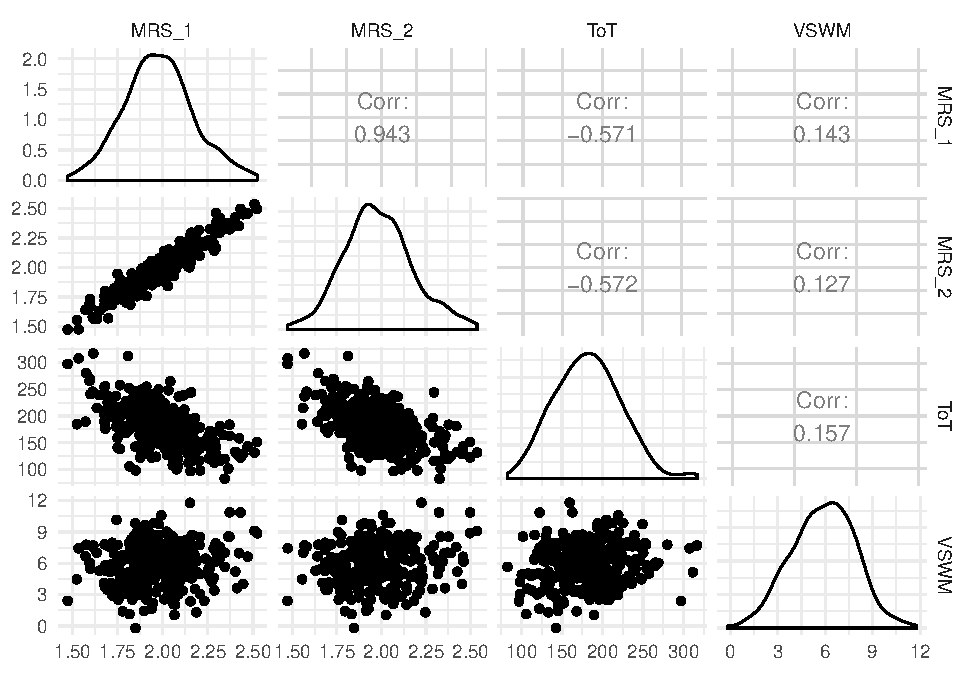
\includegraphics{Bayesian_statistics_files/figure-latex/unnamed-chunk-27-1.pdf}

\begin{Shaded}
\begin{Highlighting}[]
\KeywordTok{grid.arrange}\NormalTok{(}
\NormalTok{  D_psychomet }\OperatorTok\StringTok{  }\KeywordTok{ggcov}\NormalTok{(MRS_}\DecValTok{1}\NormalTok{, MRS_}\DecValTok{2}\NormalTok{)  }\OperatorTok{+}\StringTok{ }
\StringTok{    }\KeywordTok{theme}\NormalTok{(}\DataTypeTok{legend.justification=}\KeywordTok{c}\NormalTok{(}\DecValTok{1}\NormalTok{,}\DecValTok{0}\NormalTok{), }\DataTypeTok{legend.position=}\KeywordTok{c}\NormalTok{(}\DecValTok{1}\NormalTok{,}\DecValTok{0}\NormalTok{)),}
\NormalTok{  D_psychomet }\OperatorTok\StringTok{  }\KeywordTok{ggcov}\NormalTok{(MRS_}\DecValTok{1}\NormalTok{, ToT),}
\NormalTok{  D_psychomet }\OperatorTok\StringTok{  }\KeywordTok{ggcov}\NormalTok{(MRS_}\DecValTok{1}\NormalTok{, VSWM),}
  \DataTypeTok{ncol =} \DecValTok{3}
\NormalTok{)}
\end{Highlighting}
\end{Shaded}

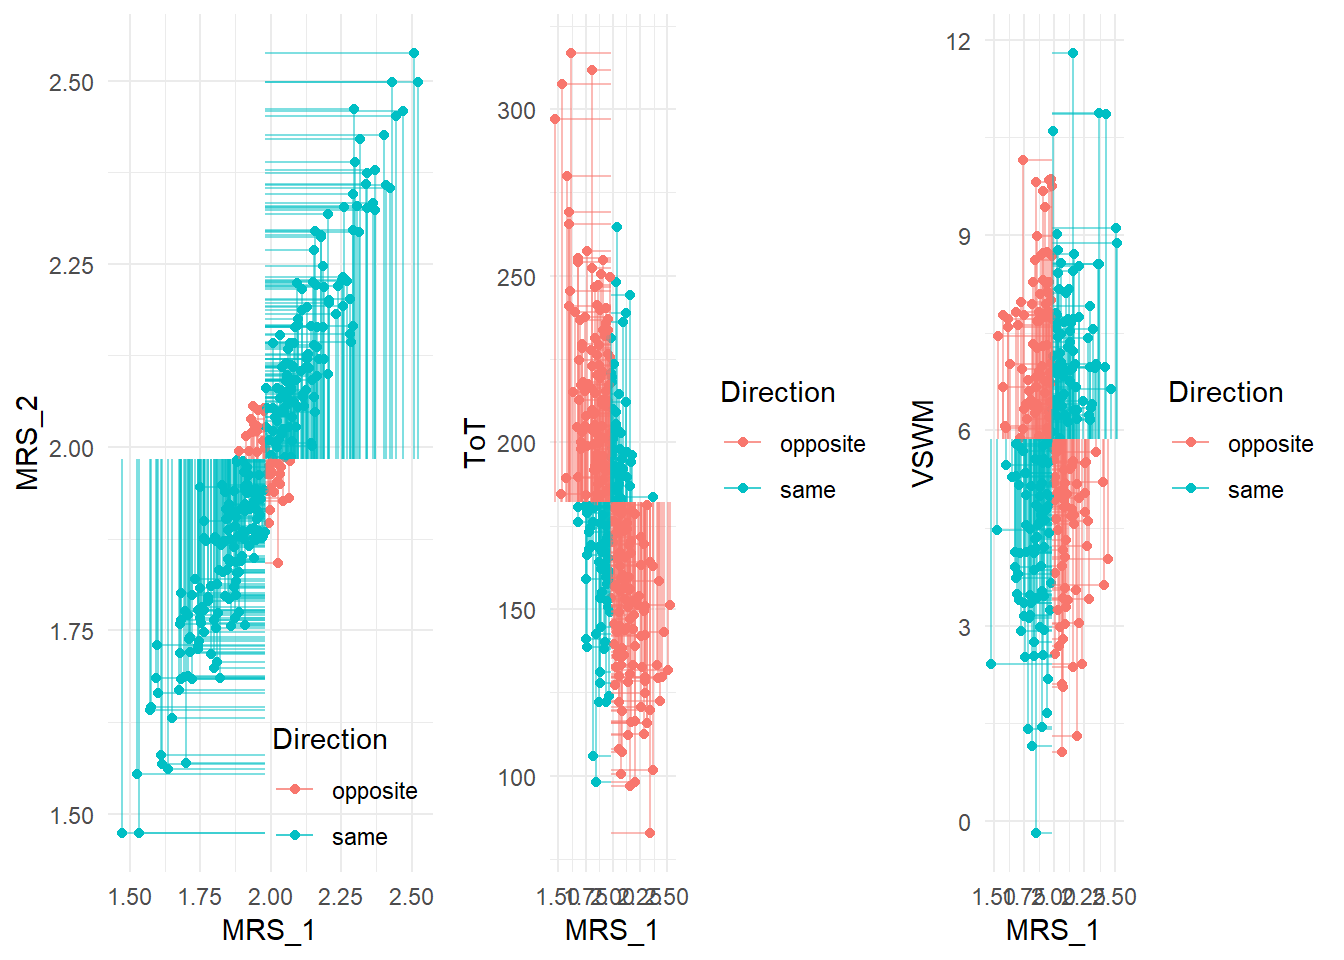
\includegraphics{Bayesian_statistics_files/figure-latex/unnamed-chunk-27-2.pdf}

The graphs highlight the deviation from the population mean of each
variables. A strong covariance emerges whenever there is a strong
tendency to deviate in either one direction. In fact, the illustration
introduces a geometric interpretation: every data point stretches a
rectangle which has an area of the product of the two deviations, just
like in the formula of covariance.

As intuitive the idea of covariance is, as unintelligible is the
statistic itself for reporting results. Covariance is not a pure measure
of association, but is contaminated by the dispersions of \(X\) and
\(Y\). For that reason, two covariances can hardly be compared. The
\emph{Pearson correlation coefficient} \(r\) solves the problem by
rescaling a covariance by the two standard deviations:

\[
r_XY = \frac{\textrm{cov}_{XY}}{\textrm{sd}_X \textrm{sd}_Y}
\]

\begin{Shaded}
\begin{Highlighting}[]
\NormalTok{cor <-}\StringTok{ }\ControlFlowTok{function}\NormalTok{(x, y)}
  \KeywordTok{cov}\NormalTok{(x, y)}\OperatorTok{/}\NormalTok{(}\KeywordTok{sd}\NormalTok{(x, }\DataTypeTok{na.rm =}\NormalTok{ T) }\OperatorTok{*}\StringTok{ }\KeywordTok{sd}\NormalTok{(y, }\DataTypeTok{na.rm =}\NormalTok{ T))}

\KeywordTok{cor}\NormalTok{(D_psychomet}\OperatorTok{$}\NormalTok{MRS_}\DecValTok{1}\NormalTok{, D_psychomet}\OperatorTok{$}\NormalTok{MRS_}\DecValTok{2}\NormalTok{)}
\end{Highlighting}
\end{Shaded}

\begin{verbatim}
## [1] 0.943
\end{verbatim}

Due to the standardization of dispersion, \(r\) lets the researcher
interpret strength of association independent of scale of measurement.
More precisely, \(r\) will always be in the interval \([-1,1]\). That
makes it the perfect choice for several purposes.

In the field of psychometrics, correlations are ubiquotously employed to
represent \emph{reliability} and \emph{validity} of tests. For example,
when the long-term career of an individual is dependent on the score of
an assessment, it would be inexceptable if test scores differed strongly
from day to day. \emph{Test-retest stability} is one form to measure
reliability and it is just the correlation of the same test taken on
different days. For example, we could ask whether mental rotation speed
as measured by the mental rotation task is a stable, such that we can
use it for long-term predictions of whether someone will become a good
surgeon. A reliability of \(.95\) will probably satisfy most
psychometricians. Validity of a test means that it predicts what it was
intended for. For example, we could ask how well the ability of a person
to become a minimally invasive surgeon depends on spatial cognitive
abilities, like mental rotation speed. Validity could be assessed by
taking performance scores from exercises in a surgery simulator and do
the correlation with mental rotation speed. A correlation of \(r = .5\)
would indicate that mental rotation speed as measured by the task has
rather limited validity. Another form is called \emph{discriminant
validity} and is about how specific a measure is. Imagine another test
is already part of the assessment suite. This test aims to measure
another aspect of spatial cognition, namely the capacity of the
visual-spatial working memory (e.g., the Corsi block tapping task). If
both tests are as specific as they claim to be, we would expect a
particularly low correlation.

\begin{Shaded}
\begin{Highlighting}[]
\NormalTok{D_psychomet }\OperatorTok\StringTok{ }
\StringTok{  }\NormalTok{GGally}\OperatorTok{::}\KeywordTok{ggpairs}\NormalTok{()}
\end{Highlighting}
\end{Shaded}

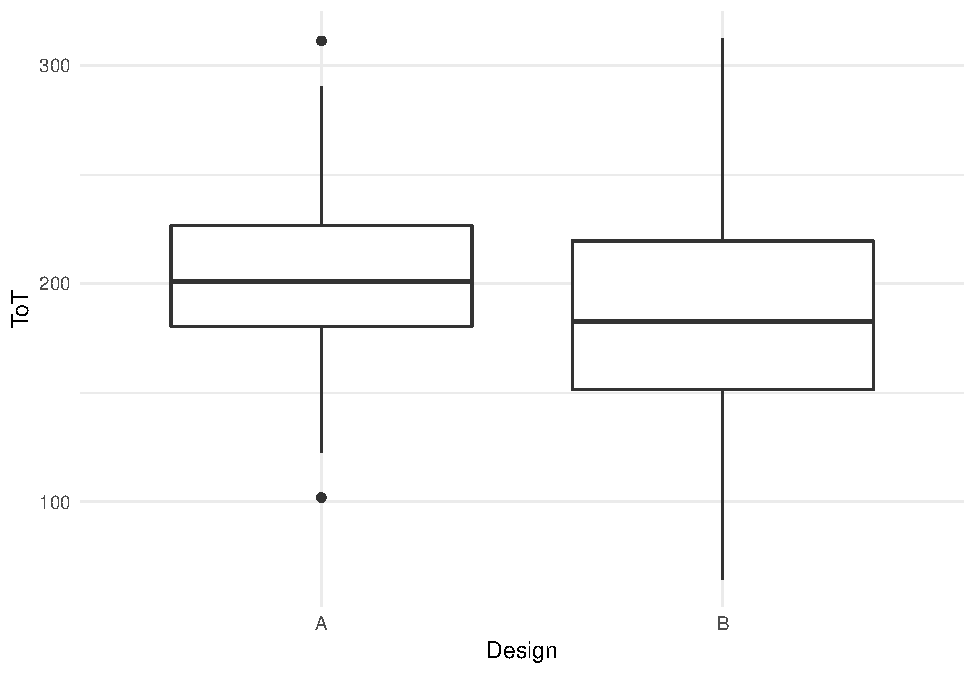
\includegraphics{Bayesian_statistics_files/figure-latex/unnamed-chunk-30-1.pdf}

Correlations allow psychometricians to employ absolute standards for the
quality of measures. In exploratory analysis, one often seeks to get a
broad overview of how a bunch of variables is associated. Creating a
correlation table of all variables is no hassle and allows to get a
broad picture of the situation. Correlations are ubitutous in data
analysis, but have limitations: First, a correlation only uncovers
linear trends, whereas the association between two variables can take
any conceivable form. The validity of correlations depends on how
salient the feature of linear trend is. In the example below, \(Y_1\)
reveals a strong parabolic form, which results in zero correlation. The
curvature of an exponentially rising function is only captured
insufficiently. For that reason, I recommend that correlations are
always cross-checked by a scatterplot.

Another situation where covariances and correlations fail is when there
simply is no variance. It is almost trivial, but for observing how a
variable \(Y\) changes when \(X\) moves is that both variables
\emph{vary}, there is no co-variance without variance.

\begin{Shaded}
\begin{Highlighting}[]
\KeywordTok{data_frame}\NormalTok{(}\DataTypeTok{x =}\NormalTok{  (}\DecValTok{0}\OperatorTok{:}\DecValTok{100}\NormalTok{)}\OperatorTok{/}\DecValTok{10}\NormalTok{,}
           \DataTypeTok{y_1 =} \KeywordTok{rnorm}\NormalTok{(}\DecValTok{101}\NormalTok{, }\KeywordTok{exp}\NormalTok{(x)}\OperatorTok{/}\DecValTok{100}\NormalTok{, x }\OperatorTok{*}\StringTok{ }\DecValTok{2}\NormalTok{),}
           \DataTypeTok{y_2 =} \KeywordTok{rnorm}\NormalTok{(}\DecValTok{101}\NormalTok{, (x }\OperatorTok{-}\StringTok{ }\DecValTok{5}\NormalTok{)}\OperatorTok{^}\DecValTok{2}\NormalTok{, }\DecValTok{3}\NormalTok{)) }\OperatorTok\StringTok{ }
\StringTok{  }\KeywordTok{ggpairs}\NormalTok{(}\DataTypeTok{lower=}\KeywordTok{list}\NormalTok{(}\DataTypeTok{continuous=}\StringTok{"smooth"}\NormalTok{))}
\end{Highlighting}
\end{Shaded}

\includegraphics{Bayesian_statistics_files/figure-latex/unnamed-chunk-31-1.pdf}

\subsubsection{{[}HERE{]}}\label{here}

\section{Bayesian Inferential
statistics}\label{bayesian-inferential-statistics}

Bayesian statistics can be reduced to three elements:

\begin{enumerate}
\def\labelenumi{\arabic{enumi}.}
\tightlist
\item
  the \emph{prior belief} is what you believe before (little rain in
  summer)
\item
  the \emph{likelihood} is what you learn by observation (the cloudy
  sky)
\item
  the \emph{posterior belief} is your adjusted believe after seeing the
  data
\end{enumerate}

Bayesian statistics formalizes the transition from prior belief to
posterior belief in a remarkably simple formula:

\[\text{posterior}\ \propto \text{prior}\times\text{likelihood}\]

Note that \(\propto\) here means \emph{proportional to}. In very plain
words this is:

\begin{quote}
what you believe now is a combination of what you knew before and what
you have just seen in the data.
\end{quote}

The data is usually the present observation or study. But, that does not
exclude that prior knowledge grounds on data, too. In experimental
Psychology researchers entertain themselves repetitions of the very same
experimental paradigm, with slight variations maybe. For example, in the
famous Stroop effect, participants have to name the ink color of a word.
When the word is itself a color word and refers to a different color,
response times typically increase. This effect has been replicated in
many dozens of published studies and, probably, thousands of student
experiments. Cumulative evidence is so strong that, would repeat the
experiment another time and find the reverse effect, no one would
seriously take this as a debunk. This extreme example illustrates
another principle that follows from Bayes rule:

\begin{quote}
Today's posterior is tomorrow's prior.
\end{quote}

There is no principled difference between prior and posterior. They are
just levels of belief (credences) at different points in time. Both
differ in strength: prior knowledge can be firm when it rests on an
abundance of past evidence. The same holds for the likelihood in the
present data: the more observations, the stronger the evidence. This is
why larger sample sizes are usually preferred. Prior belief and
likelihood can be congruent or contradict each other. When they are
congruent, prior belief is strengthened by the data. When they are
contradicting each other, prior belief is weakened.

Whatever happens in the individual case, it is generally accepted that
scientific progress is incremental over large periods of time. Under
this perspective the idea of updating one's belief is even trivial. It
is common sense, that if you are too uncertain about a situation you
better gather more information. Once you have reached a satisfactory
level of certainty, you proceed to act (or publish).

Readers with a firm background in classic statistics may (or my not)
recall that once you have settled down on a sample size (and a level of
significance), you absolutely must test precisely this number of
participants. Stopping early (because you have reached the desired
p-value) or adding to the sample is strictly forbidden. Doesn't that
bother you under the perspective of accumulative evidence? It should
bother you that incremental collection of evidence is impossible when
doing frequentist statistics. On the other hand, in Bayesian statistics,
accumulation of evidence is a core feature.

Neither is there a way to express one's prior belief when doing a
t-test, nor can you just continue your data collection until
satisfactory certainty is reached. In the fictional example of the
Stroop task, the classic data analysis pretends as if no one has ever
done such an experiment before. At the same time, it is strictly
forbidden to invite further participants to the lab, when the test
results point into the right direction, but evidence is still to weak.
If you planned the study with, say, \(N = 20\), this is what you have to
do, no less no more. If you reach your goal with less participants, you
must continue testing. If you are unsatisfied with the level of
certainty (e.g., \(p = .52\)), the only permissable action is dump your
data and start over from zero. There are many other ways that
frequentist statistics is flawed, including some deeply philosophical
ones. For a common person the denial of incremental progress is deeply
counter-intuitive and for a common researcher it is a millstone around
the neck.

Reconsider Jane and Andrew. What did they know about the current state
of affairs when running a particular session. Using some time-on-task
measures they disproved the claim ``rent a car in 99 seconds''. Recall
how precisely the question was phrased: on average, users had to be able
to complete the transaction in 99 seconds. The statistic of interest is
the mean. This was debunked with almost no effort, by calculating:

\[\hat M_{ToT} = 1 \over n * \sum{ToT} = 105.975\]

But how about the updated slogan: ``rent a car in 111 seconds''. Can we
be sure it holds, when someone repeats the study? We can only to a
degree. It could still happen, that the belligerent competitor comes to
a different result, just because they have a different sample of
participants. Even if they would test a fully matching sample of
participants, the measures will differ, simply because an array of
smaller and larger impact factors is continuously hitting the central
and peripheral nervous systems of your participants. The result is
randomness in the data. Fortunately, randomness is often found to be
well-behaved in that recurrent patterns emerge. These patterns are
called distributions of randomness and I will introduce a whole bunch of
them later in this chapter @\ref().

\subsubsection{{[}HERE{]}}\label{here-1}

\section{Bayesian probability theory}\label{bayesian-probability-theory}

Probability is an elusive concept and a source of mental suffering and
heated debates, especially when people use intuition. The reason is that
in the human mind, probability can be rooted in two different ways: in
frequentist thinking, probability is represented by relative
frequencies, whereas in Bayesian school of thought it is the level of
certainty for some event to happen.

This is a Bayesian book and the following considerations are meant to
convince the reader that the Bayesian use of probability has a wider
domain of application than the frequentist. I also see this as one of
the more rare situations where introducing some formalism is supportive
in that it dissolves the subtle preoccupations that often accompany
intuitive (or, I'd rather say: exemplified) understanding. In addition,
the mathematical definition is bare of any real world notions, like
observed frequencies or experienced certainties and (figuratively
speaking) makes the different perspectives converge. The algebraic
definition of probability is given by the three Kolmogorov axioms.
Before we come to that, let me undertake two intermediate steps: a deep
bow to the discipline of mathematics, and introducing some set-theoretic
concepts.

First, be reminded that mathematical systems of belief are empty. It
often helps, to associate a mathematical system of statements to with
some more tangible ideas. For example, I remember how my primary school
teacher introduced the sum of two numbers as moving elements from one
stack onto another, piece by piece. Later, I found this to be an exact
embodidment of how the sum follows from the Peano axioms, that define
the set of natural numbers. Second, we need to set the stage with a few
set-theoretic concepts.

\subsection{Some set theory}\label{some-set-theory}

A mathematical \emph{set} is a collection of elements taken from a
domain (or universe, more dramatically). These can either be defined by
stating all the elements, like
\(S = \{\textrm{red}, \textrm{yellow}, \textrm{green}, \textrm{off}\}\)
or by a characterizing statement, like:

\(S := \textrm{possible states of a Dutch traffic light}\)

The elements should be clearly identified, but need not have a
particular order. (If they do, this is called an \emph{ordered set}, the
set of natural numbers is an example). Sets can have all possible sizes,
which is called the \emph{cardinality} of a set:

\begin{itemize}
\tightlist
\item
  empty like all opponents who can defeat Chuck Norris, \(\{\}\) or
  \(\oslash\)
\item
  finite like the possible states of a traffic light
\item
  infinite, but countable, like the natural numbers \(N\)
\item
  infinite, uncountable, like the real numbers \(R\)
\end{itemize}

You may wonder now, whether you would ever need such a strange concept
as uncaountable infinite sets in your down-to-earth design research.
Well, the set of primary interest in every design study is the possible
outcomes. Sometimes, these are finite, like
\(\{\textrm{success}, \textrm{failure}\}\), but when you measure
durations or distances, you enter the realm of real numbers. We will set
this issue aside for the moment and return to it later in the context of
continuous distributions of randomness.

In order to introduce the mathematical concept of probability, we first
have to understand some basic operations on sets. For an illustration,
imagine a validation study for a medical infusion pump, where
participants were given a task and the outcome was classified by the
following three criteria:

\begin{itemize}
\tightlist
\item
  was the task goal achieved successfully?
\item
  was the task completed timely (e.g., one minute or below)?
\item
  were there any operation errors along the way with potentially harmful
  consequences?
\end{itemize}

\begin{longtable}[]{@{}rlll@{}}
\toprule
Obs & Timely & Harm & Success\tabularnewline
\midrule
\endhead
4 & TRUE & TRUE & FALSE\tabularnewline
6 & TRUE & TRUE & FALSE\tabularnewline
11 & TRUE & FALSE & TRUE\tabularnewline
17 & TRUE & FALSE & TRUE\tabularnewline
22 & FALSE & TRUE & FALSE\tabularnewline
23 & FALSE & TRUE & FALSE\tabularnewline
24 & FALSE & FALSE & TRUE\tabularnewline
30 & FALSE & FALSE & FALSE\tabularnewline
\bottomrule
\end{longtable}

Note how the the data table makes use of logical values to denote their
membership to a set. Based on these three criteria, we can extract
subsets of observations:

\begin{Shaded}
\begin{Highlighting}[]
\KeywordTok{library}\NormalTok{(sets)}
\end{Highlighting}
\end{Shaded}

\begin{Shaded}
\begin{Highlighting}[]
\NormalTok{All      <-}\StringTok{ }\KeywordTok{as.set}\NormalTok{(D_sets}\OperatorTok{$}\NormalTok{Obs)}
\NormalTok{Success  <-}\StringTok{ }\KeywordTok{as.set}\NormalTok{(}\KeywordTok{filter}\NormalTok{(D_sets, Success)}\OperatorTok{$}\NormalTok{Obs)}
\NormalTok{Harmful  <-}\StringTok{ }\KeywordTok{as.set}\NormalTok{(}\KeywordTok{filter}\NormalTok{(D_sets, Harm)}\OperatorTok{$}\NormalTok{Obs)}
\NormalTok{Timely   <-}\StringTok{ }\KeywordTok{as.set}\NormalTok{(}\KeywordTok{filter}\NormalTok{(D_sets, Timely)}\OperatorTok{$}\NormalTok{Obs)}
\end{Highlighting}
\end{Shaded}

The first basic set operator is the \emph{complementary set}. It selects
all elements from the domain that are not part of a given set:

\begin{Shaded}
\begin{Highlighting}[]
\NormalTok{Failure  <-}\StringTok{ }\NormalTok{All }\OperatorTok{-}\StringTok{ }\NormalTok{Success}
\NormalTok{Harmless <-}\StringTok{ }\NormalTok{All }\OperatorTok{-}\StringTok{ }\NormalTok{Harmful}
\NormalTok{Delayed  <-}\StringTok{ }\NormalTok{All }\OperatorTok{-}\StringTok{ }\NormalTok{Timely}
\end{Highlighting}
\end{Shaded}

Once there is more than one set in the game, set operators can be used
to create all kinds of new sets. First, the \emph{union} of two sets
collects the elements of two separate sets into one new set, for
example, the set of all tasks that were failure or delayed (or both):

\begin{Shaded}
\begin{Highlighting}[]
\NormalTok{Failure }\OperatorTok{|}\StringTok{ }\NormalTok{Delayed}
\end{Highlighting}
\end{Shaded}

\begin{verbatim}
## {1L, 2L, 3L, 4L, 5L, 6L, 19L, 20L, 21L, 22L, 23L, 24L, 25L, 26L,
##  27L, 28L, 29L, 30L}
\end{verbatim}

Another commonly used set operator is the \emph{intersect}, which
produces a set that contains only those elements present in both
original sets, like the set of timely and succesful task completions:

\begin{Shaded}
\begin{Highlighting}[]
\NormalTok{Success }\OperatorTok{&}\StringTok{ }\NormalTok{Timely}
\end{Highlighting}
\end{Shaded}

\begin{verbatim}
## {7L, 8L, 9L, 10L, 11L, 12L, 13L, 14L, 15L, 16L, 17L, 18L}
\end{verbatim}

The \emph{set difference} removes elements of one set from another, for
example the set of all successful observations with no harmful side
effects:

\begin{Shaded}
\begin{Highlighting}[]
\NormalTok{Success }\OperatorTok{-}\StringTok{ }\NormalTok{Harmless}
\end{Highlighting}
\end{Shaded}

\begin{verbatim}
## {}
\end{verbatim}

It turns out that all succesful observations are also harmless. That
indicates that the set of successful events is a \emph{subset} of
harmless events. The subset operator differs from those discussed so
far, in that it does not produce a new set, but a truth value (also
called logical or Boolean). A distinction is made between subsets and
\emph{proper subsets}, where one set contains all elements of another,
but never the other way round. If two sets are mutual subsets (and
therefore improper), they are \emph{equal}.

\begin{Shaded}
\begin{Highlighting}[]
\CommentTok{# subset}
\NormalTok{Success }\OperatorTok{<=}\StringTok{ }\NormalTok{Harmless}
\end{Highlighting}
\end{Shaded}

\begin{verbatim}
## [1] TRUE
\end{verbatim}

\begin{Shaded}
\begin{Highlighting}[]
\CommentTok{# proper subset}
\NormalTok{Success }\OperatorTok{<}\StringTok{ }\NormalTok{Harmless}
\end{Highlighting}
\end{Shaded}

\begin{verbatim}
## [1] TRUE
\end{verbatim}

\begin{Shaded}
\begin{Highlighting}[]
\CommentTok{# set equality}
\NormalTok{Success }\OperatorTok{==}\StringTok{ }\NormalTok{Harmless}
\end{Highlighting}
\end{Shaded}

\begin{verbatim}
## [1] FALSE
\end{verbatim}

\begin{Shaded}
\begin{Highlighting}[]
\NormalTok{Success }\OperatorTok{==}\StringTok{ }\NormalTok{(All }\OperatorTok{-}\StringTok{ }\NormalTok{Failure)}
\end{Highlighting}
\end{Shaded}

\begin{verbatim}
## [1] TRUE
\end{verbatim}

The example above demonstrates another important element of set theory:
the empty set, which has the special property of being a subset of all
other set:

\begin{Shaded}
\begin{Highlighting}[]
\KeywordTok{set}\NormalTok{() }\OperatorTok{<}\StringTok{ }\NormalTok{Success}
\end{Highlighting}
\end{Shaded}

\begin{verbatim}
## [1] TRUE
\end{verbatim}

Among other uses, the empty set is important for intersections. It may
happen that two sets do not share any elements at all. It would be
problematic, if the intersect operator only worked if common elements
truly existed. In such a case, the intersection of two sets is the empty
set. Sets that have an empty intersection are called \emph{disjunct
sets} and complementary sets are a special case. The package Sets, which
defines all operators on sets so far is lacking a dedicated function for
disjunctness, but this is easily defined using the intersect function:

\begin{Shaded}
\begin{Highlighting}[]
\NormalTok{is_disjunct <-}\StringTok{ }\ControlFlowTok{function}\NormalTok{(x, y) }\KeywordTok{set_is_empty}\NormalTok{(x }\OperatorTok{&}\StringTok{ }\NormalTok{y)}
\KeywordTok{is_disjunct}\NormalTok{(Success, Harmful)}
\end{Highlighting}
\end{Shaded}

\begin{verbatim}
## [1] TRUE
\end{verbatim}

So far, we have only seen sets of atomic elements, where all elements
are atomic, i.e.~they are not sets themselves. We can easily conceive a
set that has elements that are sets. The set of sets that are defined by
the three performance criteria and their complementary sets is an
obvious example:

\begin{Shaded}
\begin{Highlighting}[]
\KeywordTok{set}\NormalTok{(Success, Failure, Harmful, Harmless, Timely, Delayed)}
\end{Highlighting}
\end{Shaded}

\begin{verbatim}
## {<<set(9)>>, <<set(10)>>, <<set(12)>>, <<set(18)>>, <<set(20)>>,
##  <<set(21)>>}
\end{verbatim}

For the introduction of probability, we need two concepts related to
sets o sets: First, a \emph{partition of a set} is a set of non-empty
subsets such that every element is assigned to exactly one subset. The
subsets of successes and its conplementary set, all failures, is such a
partition. Second, the \emph{power set} is the set of all possible
subsets in a set. Even with a rather small set of 20 elements, this is
getting incredibly large, so let's see it on a smaller example:

\begin{Shaded}
\begin{Highlighting}[]
\NormalTok{S <-}\StringTok{ }\KeywordTok{set}\NormalTok{(}\DecValTok{1}\NormalTok{, }\DecValTok{2}\NormalTok{, }\DecValTok{3}\NormalTok{)}
\NormalTok{P <-}\StringTok{ }\KeywordTok{set_power}\NormalTok{(S)}
\end{Highlighting}
\end{Shaded}

The power set is tantamount for the definition of probability that
follows, because it has two properties: first, for every subset of
\texttt{S} it also contains the complementary set. That is called
\emph{closed under complementarity}. Second, for every pair of subsets
of \texttt{S}, \texttt{P} it also contains the union, it is \emph{closed
under union}. In the same way, power sets are also \emph{closed under
intersection}. Generally, all sets of subsets that fulfill these three
requirements are called \emph{\(\Sigma\) algebras}. The mathematical
theory of \(\Sigma\) algebras is central for the mathematical definition
of measures. Loosely speaken, a measure is a mapping from the domain of
empirical observations to the domain of numbers, such that certain
operations in the domain of measurement have their counterparts in the
numerical domain. Probabilities are measures and in the next section we
will see how numerical operations on probabilities relate to set
operations in a \(\Sigma\) algebra.

\subsection{Probability}\label{probability}

Before we get to a formal presentation of probability, we can develop
the idea on the fictional validation study introduced in the previous
section. Performance of participants was classified by the three
two-level criteria, success, harm and timeliness. Every recorded outcome
therefore falls into one of eight possible sets and a purposeful way to
summarize the results of the study would be relative frequencies
(\(\pi\), \texttt{pi}):

\begin{Shaded}
\begin{Highlighting}[]
\NormalTok{N_sets <-}\StringTok{ }\KeywordTok{nrow}\NormalTok{(D_sets)}
\NormalTok{D_freq <-}
\StringTok{  }\NormalTok{D_sets }\OperatorTok\StringTok{ }
\StringTok{  }\KeywordTok{group_by}\NormalTok{(Success, Harm, Timely) }\OperatorTok\StringTok{ }
\StringTok{  }\KeywordTok{summarize}\NormalTok{(}\DataTypeTok{n =} \KeywordTok{n}\NormalTok{()) }\OperatorTok
\StringTok{  }\KeywordTok{ungroup}\NormalTok{() }\OperatorTok\StringTok{ }
\StringTok{  }\KeywordTok{complete}\NormalTok{(Success, Harm, Timely, }\DataTypeTok{fill =} \KeywordTok{list}\NormalTok{(}\DataTypeTok{n =} \DecValTok{0}\NormalTok{)) }\OperatorTok\StringTok{ }\CommentTok{# adds empty events}
\StringTok{  }\KeywordTok{mutate}\NormalTok{(}\DataTypeTok{pi =}\NormalTok{ n}\OperatorTok{/}\KeywordTok{sum}\NormalTok{(n))}

\NormalTok{D_freq}
\end{Highlighting}
\end{Shaded}

\begin{tabular}{l|l|l|r|r}
\hline
Success & Harm & Timely & n & pi\\
\hline
FALSE & FALSE & FALSE & 1 & 0.033\\
\hline
FALSE & FALSE & TRUE & 2 & 0.067\\
\hline
FALSE & TRUE & FALSE & 3 & 0.100\\
\hline
FALSE & TRUE & TRUE & 6 & 0.200\\
\hline
TRUE & FALSE & FALSE & 6 & 0.200\\
\hline
TRUE & FALSE & TRUE & 12 & 0.400\\
\hline
TRUE & TRUE & FALSE & 0 & 0.000\\
\hline
TRUE & TRUE & TRUE & 0 & 0.000\\
\hline
\end{tabular}

Let's examine on an abstract level, what has happened here:

\begin{enumerate}
\def\labelenumi{\arabic{enumi}.}
\tightlist
\item
  The set of events has been partitioned into eight disjunct subsets
\item
  All subsets got a real number assigned, by the operation of relative
  frequencies, that is between (and including) zero and one.
\item
  The sum of these numbers is one.
\end{enumerate}

The common mathematical theory of probability assumes a set of outcomes
\(\Omega\) and a \(\Sigma\) algebra \(F\) on \(\Omega\), like the power
set. An element \(E\) of \(F\) is called an \emph{event}. Note the
difference between outcomes, which are singular outcomes, and events,
which are sets of outcomes, like the eight outcome categories above.
Also note that these eight sets are a partition of \(\Omega\), but not a
\(\Sigma\)-algebra. However, we can easily construct a
\(\Sigma\)-algebra by adding all possible unions and intersections. Or
we use the power set of outcomes in the data set right-away.

The \emph{first Kolmogorov axiom} states that a probability is a
non-negative real number assigned to every event. Take a look at the
table above, to see that this is satisfied for the relative frequencies.

While the first axiom defines a lower border of zero for a probability
measure, the \emph{second Kolmogorov axiom} cares for the upper limit
(although somewhat indirectly) by stating that the set of all
observations \(\Omega\) (which is an element of \(F\)) is assigned a
probability of one. In the table of relative frequencies that is not yet
covered, but we can easily do so:

\begin{Shaded}
\begin{Highlighting}[]
\NormalTok{D_sets }\OperatorTok
\StringTok{  }\CommentTok{# no group_by}
\StringTok{  }\KeywordTok{summarize}\NormalTok{(}\DataTypeTok{pi =} \KeywordTok{n}\NormalTok{()}\OperatorTok{/}\NormalTok{N_sets) }\OperatorTok\StringTok{ }
\StringTok{  }\KeywordTok{c}\NormalTok{()}
\end{Highlighting}
\end{Shaded}

\begin{verbatim}
## $pi
## [1] 1
\end{verbatim}

So far, the theory only cared for assigning numbers to events (subsets),
but provides no means to operate on probabilites. The \emph{third
Kolmogorov axiom} establishes a relation between the union operator on
sets and the sum operator on probabilities by stating that the
probability of a union of disjunct events is the sum of the individual
probabilities. We can approve this to be true for the relative
frequencies. For example, is the set of all successful observations is
the union of successful timely observations. Indeed, the relative
frequency of all successful events is the sum of the two and satisfies
the third axiom:

\begin{Shaded}
\begin{Highlighting}[]
\NormalTok{D_sets }\OperatorTok\StringTok{ }
\StringTok{  }\KeywordTok{group_by}\NormalTok{(Success) }\OperatorTok\StringTok{ }
\StringTok{  }\KeywordTok{summarize}\NormalTok{(}\DataTypeTok{n =} \KeywordTok{n}\NormalTok{()) }\OperatorTok\StringTok{ }
\StringTok{  }\KeywordTok{mutate}\NormalTok{(}\DataTypeTok{pi =}\NormalTok{ n}\OperatorTok{/}\KeywordTok{sum}\NormalTok{(n))}
\end{Highlighting}
\end{Shaded}

\begin{tabular}{l|r|r}
\hline
Success & n & pi\\
\hline
FALSE & 12 & 0.4\\
\hline
TRUE & 18 & 0.6\\
\hline
\end{tabular}

The Kolmogorov axioms establish a probability measure and lets us do
calculations on disjunct subsets. That would be a meager toolbox to do
calculations with probabilities. What about all the other set operators
and their possible counterparts in the realm of numbers? It is one of
greatest wonders of the human mind that the rich field of reasoning
about probabilities spawns from just these three axioms and a few set
theoretic underpinnings. To give just one example, we can derive that
the probability of the complement of a set \(A\) is
\(P(\Omega/A) = 1 - P(A)\):

\begin{enumerate}
\def\labelenumi{\arabic{enumi}.}
\item
  From set theory follows that a set \(A\) and its complement
  \(\Omega/A\) are disjunct, hence axiom 3 is applicable:
  \(P(A \cup \Omega/A) = P(A) + P(\Omega/A)\)
\item
  From set theory follows that a set \(A\) and its complement
  \(\Omega/A\) form a partition on \(\Omega\). Using axiom 2, we can
  infer: \[\begin{aligned}
  A \cup \Omega/A = \Omega\\ 
  \Rightarrow P(A) + P(\Omega/A) = P(\Omega) = 1\\ 
  \Rightarrow P(\Omega/A) = 1 - P(A)
  \end{aligned}\]
\end{enumerate}

The third axiom tells us how to deal with probabilities, when events are
disjunct. As we have seen, it applies for defining more general events.
How about the opposite direction, calculating probabilities of more
special events? In our example, two rather general events are Success
and Timely, whereas the intersection event Success \emph{and} Timely is
more special. The probability of two events occuring together is called
\emph{joint probability} \(P(\textrm{Timely} \cap \textrm{Success})\).
The four joint probabilities on the two sets and their complements are
shown in the following table.

\begin{Shaded}
\begin{Highlighting}[]
\NormalTok{D_sets }\OperatorTok\StringTok{ }
\StringTok{  }\KeywordTok{group_by}\NormalTok{(Success, Timely) }\OperatorTok\StringTok{ }
\StringTok{  }\KeywordTok{summarize}\NormalTok{(}\DataTypeTok{pi =} \KeywordTok{n}\NormalTok{()}\OperatorTok{/}\NormalTok{N_sets) }\OperatorTok\StringTok{ }
\StringTok{  }\KeywordTok{ungroup}\NormalTok{()}
\end{Highlighting}
\end{Shaded}

\begin{tabular}{l|l|r}
\hline
Success & Timely & pi\\
\hline
FALSE & FALSE & 0.133\\
\hline
FALSE & TRUE & 0.267\\
\hline
TRUE & FALSE & 0.200\\
\hline
TRUE & TRUE & 0.400\\
\hline
\end{tabular}

As joint probability asks for simultaneous occurance it treats both
involved sets symmetrically:
\(P(\textrm{Timely} \cap \textrm{Success}) = P(\textrm{Successes} \cap \textrm{Timely})\).
What if you are given one piece of information first, such as ``this was
a successful outcome'' and you have to guess the other ``Was it
harmful?''. That is called \emph{conditional probability} and in this
case, we even have 100\% certainty in our guess, because an observation
was only rated a success if there was no harm. But we can easily think
of more gradual ways to make a better guess.

\(P(\textrm{Harmful}|\textrm{Success})\)

\begin{Shaded}
\begin{Highlighting}[]
\NormalTok{D_sets }\OperatorTok
\StringTok{  }\KeywordTok{filter}\NormalTok{(Success) }\OperatorTok\StringTok{ }
\StringTok{  }\KeywordTok{group_by}\NormalTok{(Harm) }\OperatorTok\StringTok{ }
\StringTok{  }\KeywordTok{summarize}\NormalTok{(}\DataTypeTok{n =} \KeywordTok{n}\NormalTok{()) }\OperatorTok\StringTok{ }
\StringTok{  }\KeywordTok{mutate}\NormalTok{(}\DataTypeTok{pi =}\NormalTok{ n}\OperatorTok{/}\KeywordTok{sum}\NormalTok{(n)) }\OperatorTok\StringTok{ }
\StringTok{  }\KeywordTok{ungroup}\NormalTok{()}
\end{Highlighting}
\end{Shaded}

\begin{tabular}{l|r|r}
\hline
Harm & n & pi\\
\hline
FALSE & 18 & 1\\
\hline
\end{tabular}

Perhaps, there is a relationship between Timely and Harm in the manner
of a speed-accuracy trade-off. In the manner of a speed-accuracy
trade-off, there could be a relationship between Timely and Harm.
Participants who rush through the task are likely to make more harmful
errors. We would then expect a different distribution of probability of
harm by whether or not task completion was timely.

\begin{Shaded}
\begin{Highlighting}[]
\NormalTok{D_sets }\OperatorTok
\StringTok{  }\KeywordTok{group_by}\NormalTok{(Timely, Harm) }\OperatorTok\StringTok{ }
\StringTok{  }\KeywordTok{summarize}\NormalTok{(}\DataTypeTok{n =} \KeywordTok{n}\NormalTok{()) }\OperatorTok\StringTok{ }
\StringTok{  }\KeywordTok{mutate}\NormalTok{(}\DataTypeTok{pi =}\NormalTok{ n}\OperatorTok{/}\KeywordTok{sum}\NormalTok{(n)) }\OperatorTok\StringTok{ }
\StringTok{  }\KeywordTok{ungroup}\NormalTok{()}
\end{Highlighting}
\end{Shaded}

\begin{tabular}{l|l|r|r}
\hline
Timely & Harm & n & pi\\
\hline
FALSE & FALSE & 7 & 0.7\\
\hline
FALSE & TRUE & 3 & 0.3\\
\hline
TRUE & FALSE & 14 & 0.7\\
\hline
TRUE & TRUE & 6 & 0.3\\
\hline
\end{tabular}

See how conditional probabilities sum up to one \emph{within} their
condition. In this case, the conditional probabilities for harm are the
same for successes and failures. As a consequence, it is also the same
as the overall probability, hence:

\[\begin{aligned}
P(\textrm{Harm} | \textrm{Timely}) = P(\textrm{No harm} | \textrm{Timely}) =
P(\textrm{Timely})
\end{aligned}\]

This sitation is called \emph{independence of events} and it means that
knowing about one variable does not help in guessing the other. In
statistics, \emph{conditional probability} is an important concept. In
particular, it will carry us away from the set theoretic interpretation
towards the Bayesian interpretation of probability as states of
knowledge.

\begin{itemize}
\tightlist
\item
  joint probability
\item
  conditional probability (events in a sequence --\textgreater{}
  knowledge of A is knowledge of B)
\item
  independence
\item
  Bayes theorem
\end{itemize}

Other definitions and basic numerical operations on probabilities can be
inferred in similar ways.

The basic operations on probability then give rise to more advanced laws
of probability:

\subsection{Certainty as probability}\label{certainty-as-probability}

Inferential statistics serves rational decision making under uncertainty
by attaching information on the \emph{level of certainty} to a parameter
of interest. A central difference between frequentist and Bayesian
statistical theory is how the elusive concept of \emph{certainty}
emerges. Frequentists just stick to the notion of relative frequencies
to express a level of certainty. A common way to express ones level of
certainty about a parameter (say, the population mean) is a
\emph{confidence interval}, which is expressed as two endpoints:

\begin{Shaded}
\begin{Highlighting}[]
\KeywordTok{attach}\NormalTok{(Sec99)}
\end{Highlighting}
\end{Shaded}

\begin{Shaded}
\begin{Highlighting}[]
\NormalTok{Ver20 }\OperatorTok\StringTok{ }
\StringTok{  }\KeywordTok{lm}\NormalTok{(ToT }\OperatorTok{~}\StringTok{ }\DecValTok{1}\NormalTok{, }\DataTypeTok{data =}\NormalTok{ .) }\OperatorTok\StringTok{ }
\StringTok{  }\KeywordTok{confint}\NormalTok{()}
\end{Highlighting}
\end{Shaded}

\begin{tabular}{l|r|r}
\hline
  & 2.5 \% & 97.5 \%\\
\hline
(Intercept) & 99.8 & 112\\
\hline
\end{tabular}

It is by convention that the 95\% confidence interval is given and its
definition is rooted in relative frequencies: \emph{The 95\% confidence
interval is constructed in such a way that, if the same experiment were
repeated an infinite number of times, in 95\% of these repetitions the
true value is contained.}

As much as I embrace parsimony, you are not alone when you lack
intuition of what the definition says and when you feel at unease about
where all these experiments are supposed to come from. (They are all
imagined.) When we turn to Bayesian statistics, we find that it
generously elevates certainty to be a basic quantity, rather than a
derived. A Bayesian 95\% \emph{credibility interval} represents the
level of certainty as: \emph{With a probability of 95\%, the true value
is contained.} Since there seems to be no external criterion (such as a
series of experiments, imagined or not), Bayesian statistics often faced
the criticism of being subjective. In fact, if we imagine a certainty of
95\% as some number in the researchers mind, that might be true. But, it
is quite easy to grasp certainty as an objective quantity, when we
assume that there is something at stake for the researcher and that she
aims for a rational decision. In the previous chapter I have illustrated
this idea by the example of carrying an umbrella with you (or not) and
the 99 seconds claim. Generally, it helps to imagine any such situation
as a gamble: if you bet 1 EURO that the true population mean is outside
the 95\% credibility interval, as a rational person I would put 19 EUR
against.

In effect, the Bayesian concept of certainty is a probability in
mathematical terms, which liberates our reasoning from the requirement
to think of long-running series of the same experiment. Let's face the
truth: much of the time, we have only this one shot. In the next section
we will see how probability theory is used to operate on certainties
using Bayes famous theorem.

\subsection{Bayes theorem}\label{bayes-theorem}

\section{Statistical models}\label{statistical-models}

It is a scientific principle that every event to happen has its causes
(from the same universe). The better these causes are understood, the
better will be all predictions of what is going to happen the next
moment, given that one knows the laws of physics. \emph{Laplace demon}
is a classic experiment of thought on the issue: the demon is said to
have perfect knowledge of laws of physics and about the universe's
current state. Within naturalistic thinking, the demon should be able to
perfectly predict what is going to happen next. Of course, such an
entity could never exist, because it were actually a computer that
matches the universe in size. In addition, there are limits to how
precisely we can measure the current state, although physicist and
engineers have pushed this very far.

When Violet did her experiment to prove the superiority of design B, the
only two things she knew about the state of affairs was that the
participant sitting in front of her is member of a very loose group of
people called the ``typical user'' and the design her or she was exposed
to. That is painstakingly little to pin down the neural state of
affairs. Her lack of knowledge is profound but still not a problem as
the research question was gross, too, not asking for more than the
difference in \emph{average} duration. Instead, imagine Violet and a
collegue had invented a silly game where they both guess the
time-on-task of individual participants. Who comes closest wins. As both
players are clever people, they do not just randomly announce numbers,
but let themselves guide by data of previous sessions. A very simple but
reasonable approach would be to always guess the average ToT in all
previous sessions. As gross as this is, it qualifies as a model, more
precisely the grand mean model {[}LM{]}. The model explains all
observations by the population mean.

Of course, Violet would never expect her grand mean model to precisely
predict the outcome of a session. Still, imagine a device that has
perfect knowledge of the car rental website, the complete current neural
state of a the participant and the physical environment both are in. The
device would also have a complete and valid psychological theory. With
this device, Jane could always make a perfect prediction of the outcome.
Unfortunately, real design researchers are far from Laplace demoism.
Routinely borrowing instruments from social sciences, precision of
measurement is humble and the understanding of neural processes during
web navigation is highly incomplete. Participants vary in many complex
ways in their neural state and a myriad of \emph{small unrelated forces
(SMURF)} can push or hinder the user towards completion.

Laplace demon has perfect knowledge of all SMURF trajectories and
therefore can produce a perfect prediction. Violet is completely
ignorant of any SMURFs and her predictions will be off many times. A
common way to conceive this situation is that observed values \(y_i\)
are composed of the \emph{expected value} under the model \(\mu_i\) and
a \emph{random part}, \(\epsilon_i\)

\[y_i = \mu_i + \epsilon_i\]

Generally, statistical models consist of these two parts: the
\emph{likelihood} to describe the association between predictors and
expected values and the random part, which describes the overall
influence of the unexplained SMURFs.

\subsection{Predictions and
likelihood}\label{predictions-and-likelihood}

The likelihood function states the dependency of outcome on the
predictor variables. The dependency can be a complex mathematical
function of multiple predictors, or as simple as the population average.
A common likelihood function is the linear function. For example, in
their guessing game, Violet could try to improve her population model,
by also taking age of participants into account. Older people tend to be
slower. Violet creates a plot from past records. The ellipsoid form of
the point cloud indicates that ToT is somehow depending on age. Violet
draws a straight line with an upward slope to approximate the
relationship. It seems that 30 year old persons have an average ToT of
around 90 seconds, which increases to around 120 seconds for 50 year
olds. Arithmetically, this is an increase of around 1.5 seconds per year
of age.

\begin{Shaded}
\begin{Highlighting}[]
\NormalTok{Sec99}\OperatorTok{$}\NormalTok{Ver20 }\OperatorTok\StringTok{ }
\StringTok{  }\KeywordTok{ggplot}\NormalTok{(}\KeywordTok{aes}\NormalTok{(}\DataTypeTok{x =}\NormalTok{ age, }\DataTypeTok{y =}\NormalTok{ ToT)) }\OperatorTok{+}
\StringTok{  }\KeywordTok{geom_point}\NormalTok{() }\OperatorTok{+}
\StringTok{  }\KeywordTok{geom_smooth}\NormalTok{(}\DataTypeTok{method =} \StringTok{"lm"}\NormalTok{, }\DataTypeTok{se =}\NormalTok{ F)}
\end{Highlighting}
\end{Shaded}

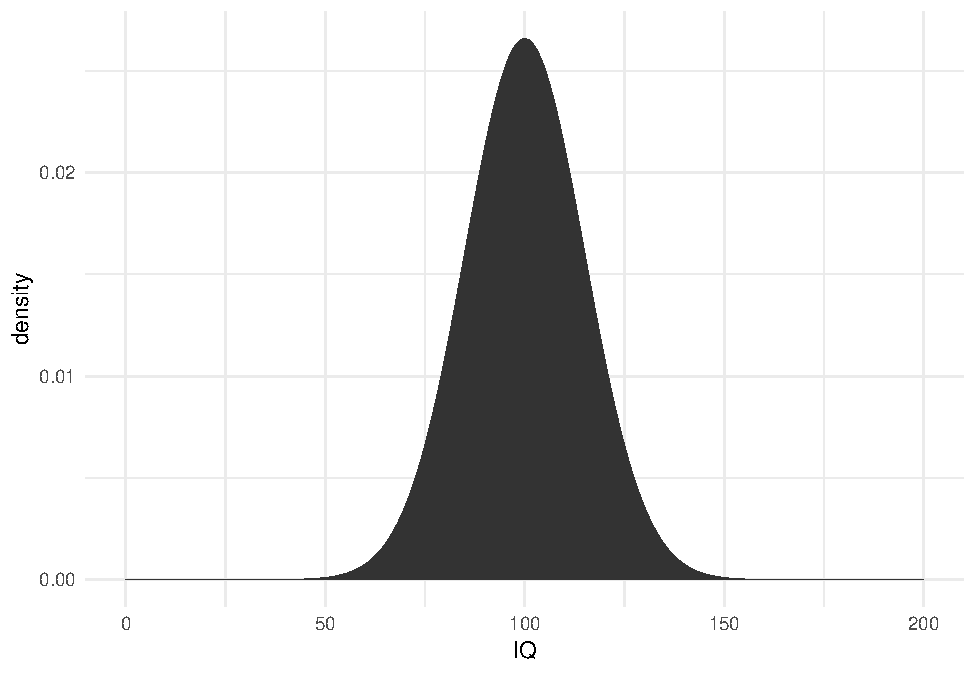
\includegraphics{Bayesian_statistics_files/figure-latex/unnamed-chunk-54-1.pdf}

Violet can use this information to improve her gambling. Instead of
stoically calling the population mean, she uses a linear function as
predictor: \$90 + (\textrm{age} - 30) 1.5 \$. In Bayesian statistics,
this is called a \emph{likelihood function} and the general form for a
single linear likelihood function is:

\[\mu_i = \beta_0 + \beta_1x_{1i}\\\]

Likelihood functions connect the \emph{expected value} \(\mu\) with
\emph{observed variables} \(x_{i1}, x_{i2}, ..., x_{ik}\), and (to be
estimated) parameters, e.g. \(\beta_0, \beta_1\). The likelihood
function is often called the \emph{deterministic part} of a model,
because its prediction strictly depends on the observed values and the
predictors, but nothing else. For example, two persons of age 30 will
always be predicted to use up 90 seconds. Apparently, this is not the
case for real data.

The linear model is very common in statistical modelling, but
likelihoods can basically take all mathematical forms. For example:

\begin{itemize}
\tightlist
\item
  the grand mean model, Violet used before: \(\mu_i = \beta_0\)
\item
  two predictors with a linear relationship:
  \(\mu_i = \beta_0 + \beta_1x_{1i} + \beta_1x_{2i}\\\)
\item
  a parabolic relationship:
  \(\mu_i = \beta_0 + \beta_1x_{1i} + \beta_2x_{2i}^2\)
\item
  a nonlinear learning curve:
  \(\mu_i = \beta_\textrm{asym} (1 + \exp(-\beta_\textrm{rate}(x_\textrm{training} + \beta_\textrm{pexp})))\)
\item
  the difference between groups A and B, where \(x_1\) is a membership
  (dummy) variable coded as
  \(A\rightarrow x_1:=0, B\rightarrow x_1:=1\):
  \(\mu_i = \beta_0 + \beta_1x_{1i}\)
\end{itemize}

In the vast majority of cases, the likelihood function is the
interesting part of the model, where researchers transform their
theoretical considerations or practical questions into a mathematical
form. The parameters of the likelihood function are being estimated and
answer the urging questions, such as:

\begin{itemize}
\tightlist
\item
  Is the design efficient enough? (\(\beta_0\))
\item
  By how much does performance depend on age? (\(\beta_1\))
\item
  Under which level of arousal does performance peak? (determining the
  staionary point of the parabola)
\item
  How fast people learn by training (\(\beta_\textrm{rate}\))
\item
  By how much design B is better than A (\(\beta_1\))
\end{itemize}

A subtle, but noteworthy feature of likelihood functions is that
\(\mu_i\) and \(x_i\) have indicators \(i\). Potentially, every
observation \(i\) has their own realization of predictors and gets a
unique expected value, whereas the parameters \(\beta_0, \beta_1\) asf.
are single values that apply for all observations at once. In fact, we
can conceive statistical models as operating on multiple levels, where
there is always the two: the observation level and the population level.
When introducing multi-level models, we will see how this principle
extends to more than these two levels. Another related idea is that
parameters summarizes patterns found in data. Any summary implies
repetition and that is what the likelihood expresses: the pattern that
repeats across observations and is therefore predictable.

\subsection{Distributions: patterns of randomness}\label{distributions}

The random part of a statistical model is what changes between
observation and is not predictable. When using the grand mean model, the
only information we are using is that the person is from the target
population. Everything else is left to the unobserved SMURFs and that
goes into the random part of the model. Fortunately, SMURFs don't work
completely arbitrary. Frequently, recognizable patterns of ramdomness
emerge. These patterns can be formulated mathematically as probability
and density distributions. A probability distribution is typically
characterized as a probability mass function that assigns
\emph{probabilities to outcomes}, such as:

\begin{itemize}
\tightlist
\item
  probability of \emph{task success} is \(.81\)
\item
  probability of \emph{99 seconds or better} is \(.22\)
\item
  probability of all SMURFs together pushing a persons \emph{IQ beyond
  115} is around \(.33\)
\end{itemize}

\subsubsection{Probability
distributions}\label{probability-distributions}

Probability distributions are mathematical functions that assign
probabilities to the outcome of a measured variable \(y\). Consider a
participant who is asked to complete three tasks of constant difficulty,
such that there is a chance of \(30\) percent for each one to be solved.
The outcome variable of interest is the number of correct completions
(0, 1, 2 or 3). Under idealized consitions, the following random
distribution gives the probability of every possible outcome.

\begin{Shaded}
\begin{Highlighting}[]
\NormalTok{D_three_tasks <-}\StringTok{ }
\StringTok{  }\KeywordTok{data_frame}\NormalTok{(}\DataTypeTok{y =} \DecValTok{0}\OperatorTok{:}\DecValTok{4}\NormalTok{,}
             \DataTypeTok{outcome =} \KeywordTok{as.character}\NormalTok{(y),}
             \DataTypeTok{probability =} \KeywordTok{dbinom}\NormalTok{(y, }\DataTypeTok{size =} \DecValTok{3}\NormalTok{, }\DataTypeTok{prob =} \FloatTok{0.3}\NormalTok{),}
             \DataTypeTok{cumul_prob     =} \KeywordTok{pbinom}\NormalTok{(y, }\DataTypeTok{size =} \DecValTok{3}\NormalTok{, }\DataTypeTok{prob =} \FloatTok{0.3}\NormalTok{))}


\NormalTok{D_three_tasks }\OperatorTok\StringTok{ }
\StringTok{  }\KeywordTok{ggplot}\NormalTok{(}\KeywordTok{aes}\NormalTok{(}\DataTypeTok{x =}\NormalTok{ outcome, }\DataTypeTok{y =}\NormalTok{ probability)) }\OperatorTok{+}
\StringTok{  }\KeywordTok{geom_col}\NormalTok{(}\DataTypeTok{fill =} \DecValTok{1}\NormalTok{) }\OperatorTok{+}
\StringTok{  }\KeywordTok{ylim}\NormalTok{(}\DecValTok{0}\NormalTok{,}\DecValTok{1}\NormalTok{) }\OperatorTok{+}
\StringTok{  }\KeywordTok{theme}\NormalTok{(}\DataTypeTok{legend.position=}\StringTok{"none"}\NormalTok{)}
\end{Highlighting}
\end{Shaded}

\includegraphics{Bayesian_statistics_files/figure-latex/unnamed-chunk-55-1.pdf}

Further, we observe that the most probable outcome is exactly one
correct task, which occurs with a probability of \(P(y = 1) = 0.441\).
At the same time, there is ample possibility for all failures,
\(P(y = 0) = 0.343\). We may also look at \emph{combined events}, say
the probability for less than two correct. That is precisely the sum
\(P(y \leq 1) = P(y = 0) + P(y = 1) = 0.784\).

We can bundle basic events by adding up the probabilities. An extreme
case of that is the universal event that includes all possible outcomes.
You can say with absolute certainty that the outcome is, indeed, between
zero and three and certainty means the probability is 1, or:
\(P(0 \leq y \leq 3) = 1\). As a matter of fact, all probability (and
density) distributions fulfill that property.

More precisely, the area under the PMF must be exactly one and that
brings us directly to a second form of characterizing the random
distribution: the \emph{cumulative distribution distribution (CDF)}
renders the probability for the outcome to be smaller or equal to \(y\).
In the case of discrete outcomes, this is just stacking (or summing)
over all outcomes, just as we did for \(P(y\leq1)\) above. The CDF of
the three-tasks example is shown in the graph below. We recognize the
left starting point, which is exactly \(P(y = 0)\) and observe large
jump to \(P(y \leq 1)\). Finally, at \(y \leq 3\) the function reaches
the upper limit of 1, which is full certainty.

\begin{Shaded}
\begin{Highlighting}[]
\NormalTok{D_three_tasks }\OperatorTok\StringTok{ }
\StringTok{  }\KeywordTok{ggplot}\NormalTok{(}\KeywordTok{aes}\NormalTok{(}\DataTypeTok{x =}\NormalTok{ y, }\DataTypeTok{y =}\NormalTok{ cumul_prob)) }\OperatorTok{+}
\StringTok{  }\KeywordTok{geom_step}\NormalTok{() }\OperatorTok{+}
\StringTok{  }\KeywordTok{ylim}\NormalTok{(}\DecValTok{0}\NormalTok{,}\DecValTok{1}\NormalTok{)}
\end{Highlighting}
\end{Shaded}

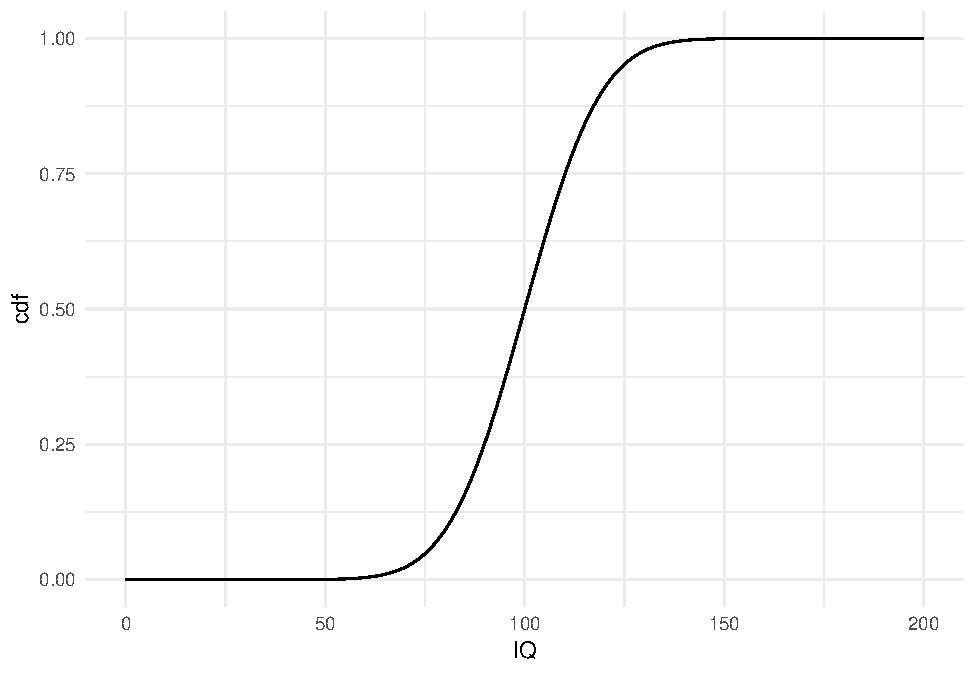
\includegraphics{Bayesian_statistics_files/figure-latex/unnamed-chunk-56-1.pdf}

\subsubsection{Density distributions}\label{density-distributions}

In the three-tasks example, reading and recombining probabilities is
like counting blocks and stacking them upon each other. This is how most
children learn basic arithmetics. when the outcome measure is
\emph{continuous}, rather than discrete, some high school math is
required. The most common continuous measure is probably durations. As
we will see, durations take quite tricky random patterns, so for the
sake of simplicity, consider the distribution of intelligence quotients
(IQ). Strictly spoken, the IQ is \emph{not} continuous, as one usually
only measures and reports whole number scores. Still, for instructional
purposes, assume that the IQ is given in arbitrary precision, be it
\(114.9\), \(100.0001\) or \(\pi * 20\).

\begin{Shaded}
\begin{Highlighting}[]
\NormalTok{D_IQ <-}\StringTok{ }\KeywordTok{data_frame}\NormalTok{(}\DataTypeTok{IQ =} \DecValTok{0}\OperatorTok{:}\DecValTok{200}\NormalTok{,}
                   \DataTypeTok{density =} \KeywordTok{dnorm}\NormalTok{(IQ, }\DecValTok{100}\NormalTok{, }\DecValTok{15}\NormalTok{),}
                   \DataTypeTok{cdf =} \KeywordTok{pnorm}\NormalTok{(IQ, }\DecValTok{100}\NormalTok{, }\DecValTok{15}\NormalTok{),}
                   \DataTypeTok{SE =}\NormalTok{ (IQ }\OperatorTok{>}\StringTok{ }\DecValTok{85}\NormalTok{) }\OperatorTok{*}\StringTok{ }\NormalTok{(IQ }\OperatorTok{<}\StringTok{ }\DecValTok{115}\NormalTok{) }\OperatorTok{*}\StringTok{ }\NormalTok{density,}
                   \DataTypeTok{PDF_085 =}\NormalTok{ (IQ }\OperatorTok{<}\StringTok{ }\DecValTok{85}\NormalTok{) }\OperatorTok{*}\StringTok{ }\NormalTok{density,}
                   \DataTypeTok{PDF_115 =}\NormalTok{ (IQ }\OperatorTok{<}\StringTok{ }\DecValTok{115}\NormalTok{) }\OperatorTok{*}\StringTok{ }\NormalTok{density)}

\NormalTok{D_IQ }\OperatorTok\StringTok{ }
\StringTok{  }\KeywordTok{ggplot}\NormalTok{(}\KeywordTok{aes}\NormalTok{(}\DataTypeTok{x =}\NormalTok{ IQ, }\DataTypeTok{y =}\NormalTok{ density)) }\OperatorTok{+}
\StringTok{  }\KeywordTok{geom_area}\NormalTok{()}
\end{Highlighting}
\end{Shaded}

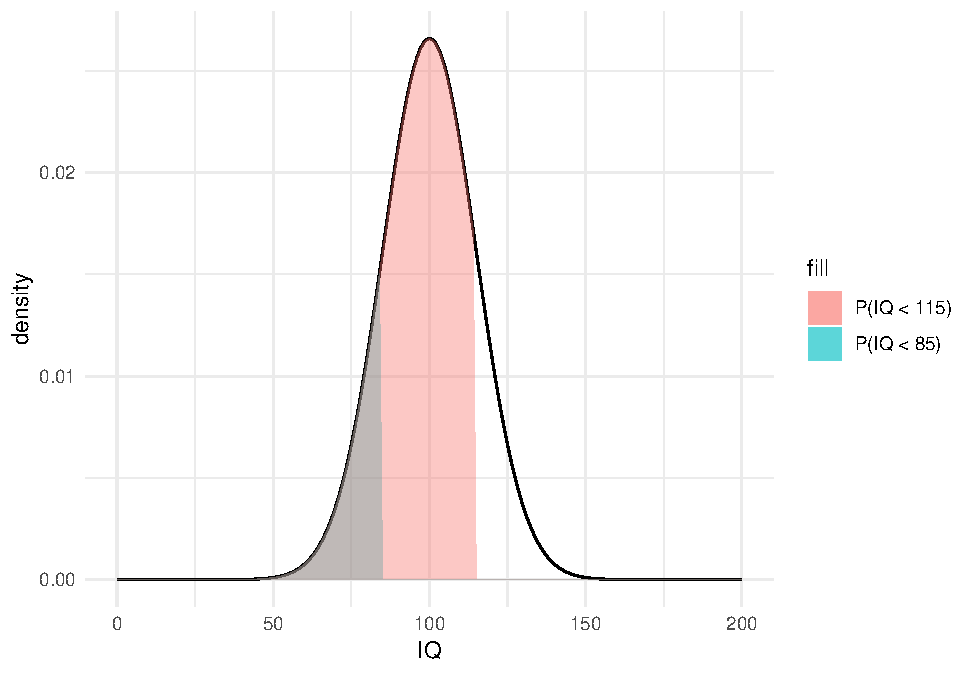
\includegraphics{Bayesian_statistics_files/figure-latex/unnamed-chunk-57-1.pdf}

We observe that the most likely IQ is 100 and that almost nobody reaches
scores higher than 150 or lower than 50. But, how likely is it to have
an IQ of exactly 100? Less than you might think! With continuous
measures, we can no longer think in blocks that have a certain area. In
fact, the probability of having an IQ of \emph{exactly} \(100.00...0\)
is exactly zero. The block of IQ = 100 is infinitely narrow and
therefore has an area of zero. Generally, with continuous outcome
variables, We can no longer read probabilities directly. Therefore,
probability mass distributions don't apply, but the association between
outcome and probability is given by what is called \emph{probability
density functions}. What PDFs share withg PMFs is that the area under
the curve is always exactly one. They differ in that PDFs return a
density for every possible outcome, which by itself is not as useful as
probability, but can be converted into probabilities.

Practically, nobody is really interested in infinite precision. When
asking \emph{``what is the probability of IQ = 100?''}, the answer is
\emph{``zero''}, but what was really meant was: \emph{``what is the
probability of an IQ in a close interval around 100?''}. Once we speak
of intervals, we clearly have areas larger than zero. The graph below
shows the area in the range of 85 to 115.

\begin{Shaded}
\begin{Highlighting}[]
\NormalTok{D_IQ }\OperatorTok\StringTok{ }
\StringTok{  }\KeywordTok{ggplot}\NormalTok{(}\KeywordTok{aes}\NormalTok{(}\DataTypeTok{x =}\NormalTok{ IQ, }\DataTypeTok{y =}\NormalTok{ density)) }\OperatorTok{+}
\StringTok{  }\KeywordTok{geom_line}\NormalTok{() }\OperatorTok{+}
\StringTok{  }\KeywordTok{geom_area}\NormalTok{(}\KeywordTok{aes}\NormalTok{(}\DataTypeTok{y =}\NormalTok{ SE))}
\end{Highlighting}
\end{Shaded}

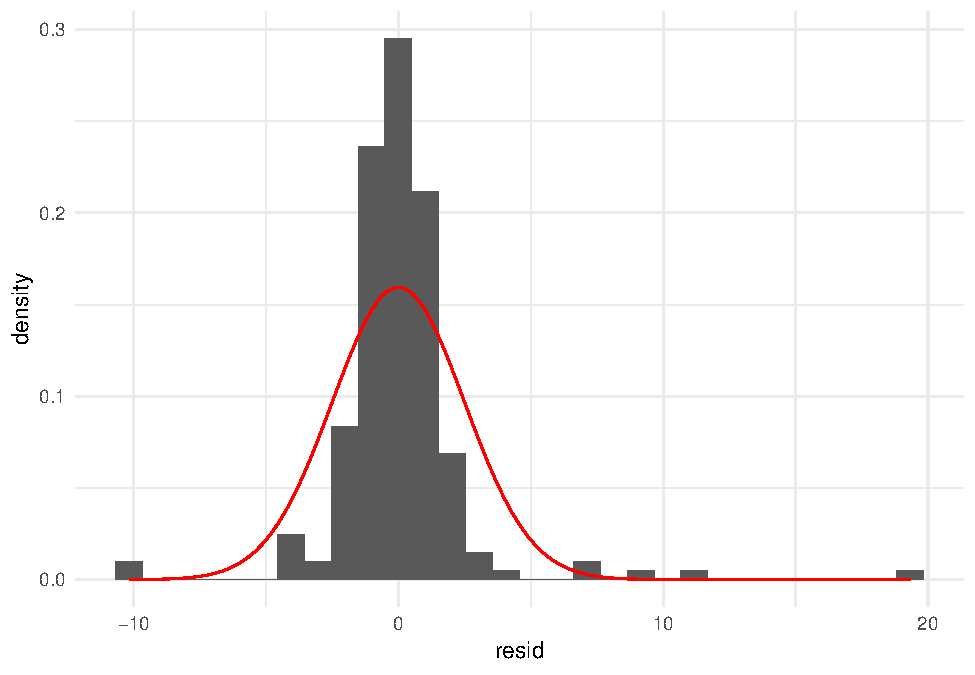
\includegraphics{Bayesian_statistics_files/figure-latex/unnamed-chunk-58-1.pdf}

But, how large is this area exactly? As the distribution is curved, we
can no longer simply count virtual blocks. Recall that the CDF gives the
probability mass, i.e.~the area under the curve, for outcomes up to a
chosen point. Continuous distributions have CDFs, too, and the the graph
below shows the CDF for the IQs. We observe how the curve starts to rise
from zero at around 50, has its steepest point at 100, just to slow down
and run against 1.

\begin{Shaded}
\begin{Highlighting}[]
\NormalTok{D_IQ }\OperatorTok\StringTok{ }
\StringTok{  }\KeywordTok{ggplot}\NormalTok{(}\KeywordTok{aes}\NormalTok{(}\DataTypeTok{x =}\NormalTok{ IQ, }\DataTypeTok{y =}\NormalTok{ cdf)) }\OperatorTok{+}
\StringTok{  }\KeywordTok{geom_line}\NormalTok{()}
\end{Highlighting}
\end{Shaded}

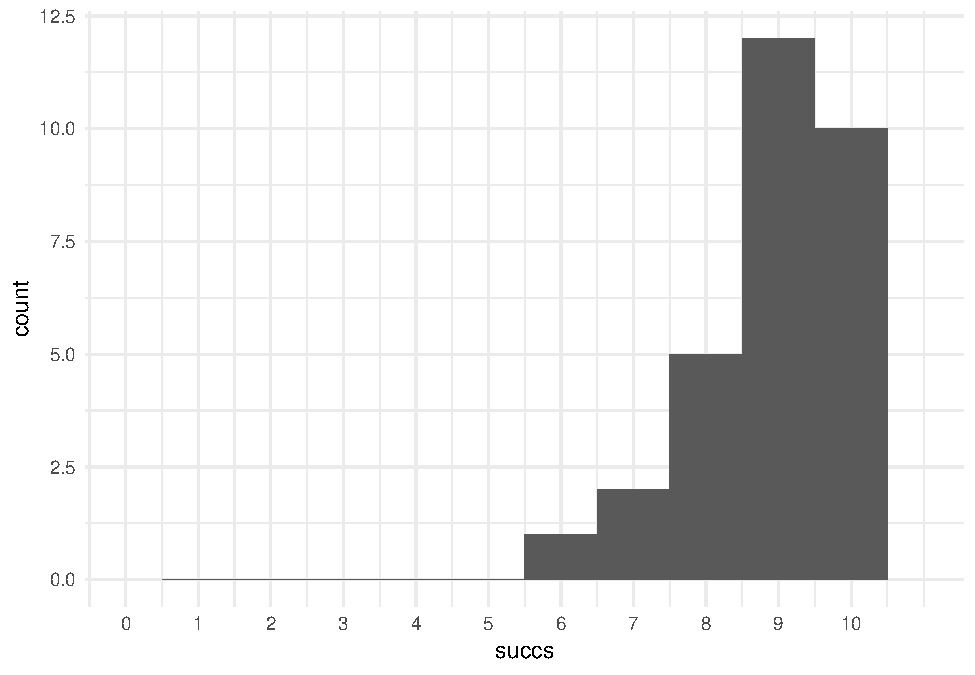
\includegraphics{Bayesian_statistics_files/figure-latex/unnamed-chunk-59-1.pdf}
Take a look at the following graph. It shows the two areas
\(IQ \leq 85\) and \(IQ \leq 115\). The magic patch in the center is
just the desired interval.

\begin{Shaded}
\begin{Highlighting}[]
\NormalTok{D_IQ }\OperatorTok\StringTok{ }
\StringTok{  }\KeywordTok{ggplot}\NormalTok{(}\KeywordTok{aes}\NormalTok{(}\DataTypeTok{x =}\NormalTok{ IQ, }\DataTypeTok{y =}\NormalTok{ density)) }\OperatorTok{+}
\StringTok{  }\KeywordTok{geom_line}\NormalTok{() }\OperatorTok{+}
\StringTok{  }\KeywordTok{geom_area}\NormalTok{(}\KeywordTok{aes}\NormalTok{(}\DataTypeTok{y =}\NormalTok{ PDF_}\DecValTok{085}\NormalTok{, }\DataTypeTok{fill =} \StringTok{"P(IQ < 85)"}\NormalTok{), }\DataTypeTok{alpha =}\NormalTok{ .}\DecValTok{4}\NormalTok{) }\OperatorTok{+}
\StringTok{  }\KeywordTok{geom_area}\NormalTok{(}\KeywordTok{aes}\NormalTok{(}\DataTypeTok{y =}\NormalTok{ PDF_}\DecValTok{115}\NormalTok{, }\DataTypeTok{fill =} \StringTok{"P(IQ < 115)"}\NormalTok{), }\DataTypeTok{alpha =}\NormalTok{ .}\DecValTok{4}\NormalTok{)}
\end{Highlighting}
\end{Shaded}

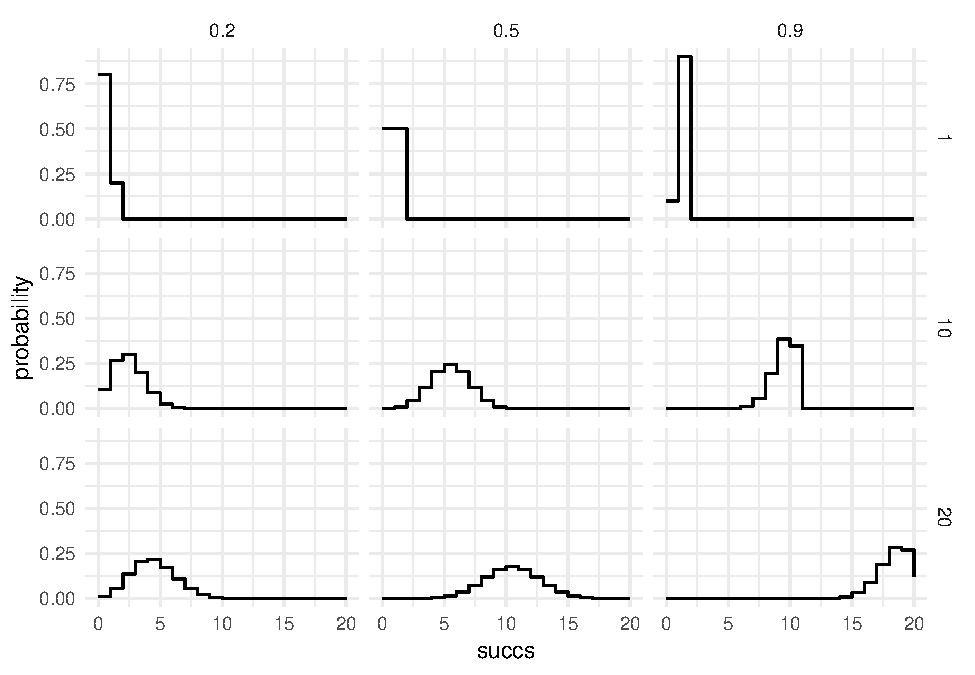
\includegraphics{Bayesian_statistics_files/figure-latex/unnamed-chunk-60-1.pdf}

And here the CDF comes into the play. To any point of the PDF, the CDF
yields the area up to this point and we can compute the area of the
interval by simple subtraction:

\[
P(IQ \leq 115) = 0.159
P(IQ \leq 85) = 0.841
P(85 \leq IQ \leq 115) = P(IQ \leq 115) - P(IQ \leq 85) = 0.683
\]

Probability and density distributions usually are expressed as
mathematical functions. For example, the function for the case of task
completion is the binomial distribution, which gives the probability for
\(y\) successes in \(k\) trials when the success rate is \(p\):

\[
Pr(y|p,k) = {k  \choose y}p^y(1-p)^{k-y}
\]

In most cases where the binomial distribution applies, base probability
\(p\) is the parameter of interest, whereas the number of of trials is
known beforehand and therefore does not require estimation. For that
reason, the binomial distribution is commonly taken as a one-parameter
distribution. When discussing the binomial in more detail, we will learn
that \(p\) determines the location of the distribution, as well as how
widely it is dispersed (preview Figure XY). The distribution that
approximated the IQs is called the Gaussian distribution (or Normal).
The Gaussian distribution function takes two parameters, \(mu\)
determines the location of the distribution, say average IQ being 98,
100 or 102 and \(sigma\) which gives the dispersion, independently
(preview Figure XY).

\subsubsection{Location and dispersion}\label{location-and-dispersion}

\emph{Location} and \emph{dispersion} are two immediate properties of
plotted distributions that have intuitive interpretations. Location of a
distribution usually reflects where the most typical values come to lie
(100 in the IQ example). When an experimenter asks for the difference of
two designs in ToT, this is purely about location. Dispersion can either
represent \emph{uncertainty} or \emph{variation} in a population,
depending on the research design and statistical model. The most common
interpretation is uncertainty. The basic problem with dispersion is that
spreading out a distribution influences \emph{how typical} the most
typical values are. The fake IQ data basically is a perfect Gaussian
distribution with a mean of 100 and a standard deviation of 15. The
density of this distribution at an IQ of 100 is 0.027. If IQs had a
standard deviation of 30, the density at 100 would fall to 0.013. If you
were in game to guess an unfamiliar persons IQ, in both cases 100 would
be the best guess, but you had a considerable higher chance of being
right, when dispersion is low.

\begin{Shaded}
\begin{Highlighting}[]
\KeywordTok{data_frame}\NormalTok{(}\DataTypeTok{IQ =} \DecValTok{0}\OperatorTok{:}\DecValTok{200}\NormalTok{,}
           \DataTypeTok{density =} \KeywordTok{dnorm}\NormalTok{(IQ, }\DecValTok{100}\NormalTok{, }\DecValTok{30}\NormalTok{)) }\OperatorTok\StringTok{ }
\StringTok{  }\KeywordTok{ggplot}\NormalTok{(}\KeywordTok{aes}\NormalTok{(}\DataTypeTok{x =}\NormalTok{ IQ, }\DataTypeTok{y =}\NormalTok{ density)) }\OperatorTok{+}
\StringTok{  }\KeywordTok{geom_area}\NormalTok{()}
\end{Highlighting}
\end{Shaded}

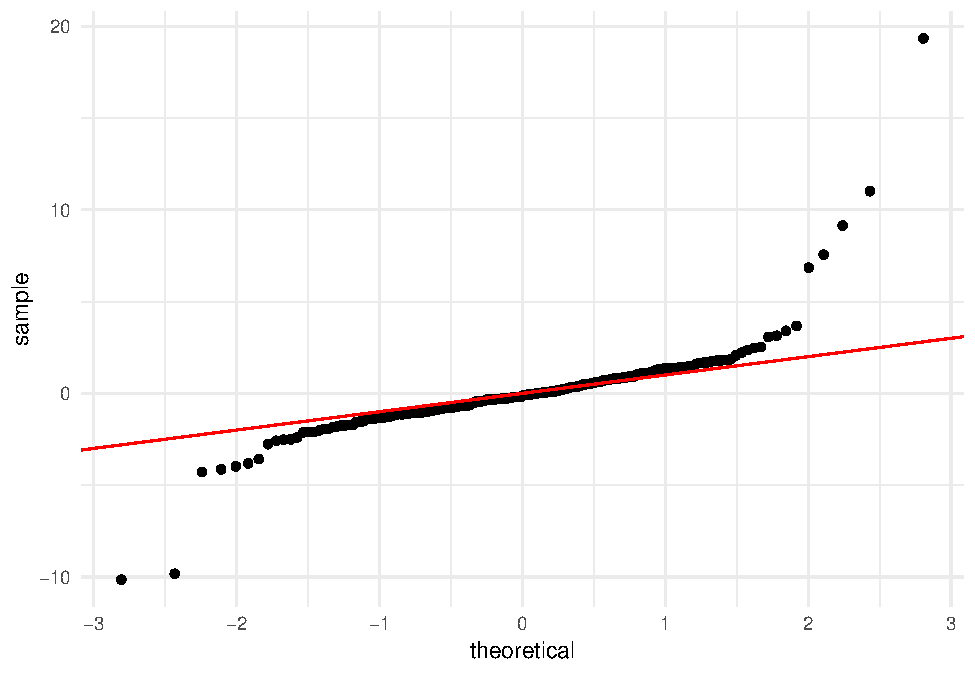
\includegraphics{Bayesian_statistics_files/figure-latex/unnamed-chunk-61-1.pdf}

The perspective of uncertainty routinely occurs in the experimental
comparison of conditions, e.g.~design A compared to design B. What
causes experimenters worry is when the \emph{residual distributions} in
their models is widely spread. Roughly speaking, residuals are the
variation that is not predicted by the model. The source of this
variation is unknown and usually called \emph{measurement error}. It
resides in the realm of the SMURFs. With stronger measurement error
dispersion, the two estimated locations get less certainty assigned,
which blurs the difference between the two.

The second perspective on dispersion is that it indicates
\emph{variation by a known source}. Frequently, this source is
differences between persons. The IQ is an extreme example of this, as
these tests are purposefully designed to have the desired distribution.
In chapter {[}LMM{]} we will encounter several sources of variation, but
I am really concerned about human variation, mostly. Commonly,
experimental researchers are obsessed by differences in location, which
to my mind confuses ``the most typical'' with ``in general''. Only when
variation by participants is low, this gradually becomes the same. We
will re-encounter this idea when turning to multi-level models.

Most distributions routinely used in statistics have one or two
parameters. Generally, if there is one parameter this determines both,
location and dispersion, whereas two-parameter distributions can vary
location and dispersion independently, to some extent. The Gaussian
distribution is a special case as \(\mu\) purely does location, whereas
\(\sigma\) is just dispersion. With common two-parametric distributions,
both parameters influence location and dispersion in more or less
twisted ways. For example, mean and variance of a two-parametric
binomial distributions both depend on chance of success \(p\) and number
of trials \(k\), as \(\textrm{M} = pk\) and \(\textrm{Var} = kp(1-p)\).

\subsubsection{Range of support and skewness {[}\#\#\#
{]}}\label{range-of-support-and-skewness}

In this book I advocate the thoughtful choice of distributions rather
than doing batteries of goodness-of-fit to confirm that one of them, the
Gaussian, is an adequate approximation. It usual is trivial to determine
whether a measure is discrete (like everything that is counted) or
(quasi)continuous and that is the most salient feature of distributions.
A second, nearly as obvious, feature of any measure is its range.
Practically all physical measures, such as duration, size or temperature
have natural lower bounds, which typically results in scales of
measurement which are non-negative. Counts have a lower boundary, too
(zero), but there can be a known upper bound, such as the number of
trials. Statistical distributions can be classified the same way: having
no bounds (Gaussian, t), one bound (usually the lower, Poisson,
exponential) or two bounds (binomial, beta).

\subsubsection{Data generating process}\label{data-generating-process}

Many dozens of PMFs and PDFs are known in statistical science and are
candidates to choose from. First orientation grounds on superficial
characteristics of measures, such as discrete/continuous or range, but
that is sometimes not sufficient. For example, the pattern of randomness
in three-tasks falls into a binomial distribution only, when all trials
have the same chance of success. If the tasks are very similar in
content and structure, learning is likely to happen and the chance of
success differs between trials. Using the binomial distribution when
chances are not constant leads to severely mistaken statistical models.

For most distributions, strict mathematical definitions exist for under
which circumstances randomness takes this particular pattern.
Frequently, there is one or more natural phenomena that accurately fall
into this pattern, such as the number of radioactive isotope cores
decaying in a certain interval (Poisson distributed) or \ldots{} . This
is particularly the case for the canonical four random distributions
that follow. Why are these canonical? The pragmatic answer is: they
cover the basic types of measures: chance of success in a number of
trials (binomial), counting (Poisson) and continuous measures
(exponential, Gaussian).

\subsubsection{Binomial distributions}\label{binomial_dist}

A very basic performance variable in design research is task success.
Think of devices in high risk sitations such as medical infusion pumps
in surgery. These devices are remarkably simple, giving a medication at
a certain rate into the bloodstream for a given time. Yet, they are
operated by humans under high pressure and must therefore be extremely
error proof in handling. Imagine, the European government would set up a
law that manufacturers of medical infusion pump must prove a 90\%
error-free operation in routine tasks. A possible validation study could
be as follows: a sample of \(N = 30\) experienced nurses are invited to
a testing lab and asked to complete ten standard tasks with the device.
The number of error-free task completions per nurse is the recorded
performance variable tpo validate the 90\% claim. Under somewhat
idealized conditions, namely that all nurses have the same proficiency
with the device and all tasks have the success chance of 90\%, the
outcome follows a \emph{Binomial distribution} and the results could
look like the following:

\begin{Shaded}
\begin{Highlighting}[]
\KeywordTok{set.seed}\NormalTok{(}\DecValTok{1}\NormalTok{)}

\KeywordTok{data_frame}\NormalTok{(}\DataTypeTok{succs =} \KeywordTok{rbinom}\NormalTok{(}\DecValTok{30}\NormalTok{, }\DecValTok{10}\NormalTok{, .}\DecValTok{9}\NormalTok{)) }\OperatorTok\StringTok{ }
\StringTok{  }\KeywordTok{ggplot}\NormalTok{(}\KeywordTok{aes}\NormalTok{(}\DataTypeTok{x =}\NormalTok{ succs)) }\OperatorTok{+}
\StringTok{  }\KeywordTok{geom_histogram}\NormalTok{(}\DataTypeTok{binwidth =} \DecValTok{1}\NormalTok{) }\OperatorTok{+}
\StringTok{  }\KeywordTok{scale_x_continuous}\NormalTok{(}\DataTypeTok{breaks =} \DecValTok{0}\OperatorTok{:}\DecValTok{10}\NormalTok{, }\DataTypeTok{limits =} \KeywordTok{c}\NormalTok{(}\DecValTok{0}\NormalTok{,}\DecValTok{11}\NormalTok{))}
\end{Highlighting}
\end{Shaded}

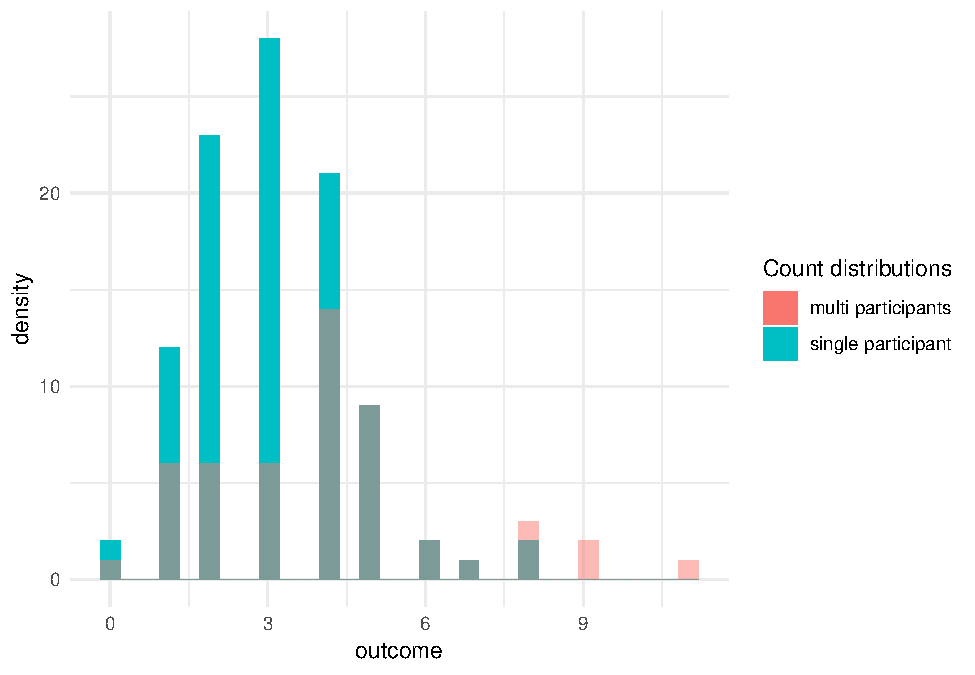
\includegraphics{Bayesian_statistics_files/figure-latex/unnamed-chunk-62-1.pdf}

Speaking about the Binomial distribution in terms of \emph{successes in
a number of attempts} is common. As a matter of fact, \emph{any} binary
classification of outcomes is amenable for Binomial modelling, like
on/off, red/blue, male/female. Imagine, Jane's big boss needs a catchy
phrase for an investor meeting. Together they decide that the return
rate of customers could be a good measure, translating into a statement
such as \emph{eighty percent of customers come back}. To prove (or
disprove) the claim, Jane uses the customer data base and divides all
individuals into two groups: those who have precisely one record and
those who returned (no matter how many times). This process results in a
distribution, that has two possible outcomes: : \(0\) for one-timers and
\(1\) for returners. This is in fact, a special case of the Binomial
distribution with \(k = 1\) attempts. Examples are given in the first
row of the figure.

\begin{Shaded}
\begin{Highlighting}[]
\NormalTok{mascutils}\OperatorTok{::}\KeywordTok{expand_grid}\NormalTok{(}\DataTypeTok{k =} \KeywordTok{c}\NormalTok{(}\DecValTok{1}\NormalTok{, }\DecValTok{10}\NormalTok{, }\DecValTok{20}\NormalTok{), }
                       \DataTypeTok{p =} \KeywordTok{c}\NormalTok{(}\FloatTok{0.2}\NormalTok{, }\FloatTok{0.5}\NormalTok{, }\FloatTok{0.9}\NormalTok{), }
                       \DataTypeTok{succs =} \DecValTok{0}\OperatorTok{:}\DecValTok{20}\NormalTok{) }\OperatorTok
\StringTok{  }\KeywordTok{mutate}\NormalTok{(}\DataTypeTok{probability =} \KeywordTok{dbinom}\NormalTok{(succs, k, p)) }\OperatorTok\StringTok{ }
\StringTok{  }\KeywordTok{ggplot}\NormalTok{(}\KeywordTok{aes}\NormalTok{(}\DataTypeTok{x =}\NormalTok{ succs, }\DataTypeTok{y =}\NormalTok{ probability)) }\OperatorTok{+}
\StringTok{  }\KeywordTok{geom_step}\NormalTok{() }\OperatorTok{+}
\StringTok{  }\KeywordTok{facet_grid}\NormalTok{(k }\OperatorTok{~}\StringTok{ }\NormalTok{p)}
\end{Highlighting}
\end{Shaded}

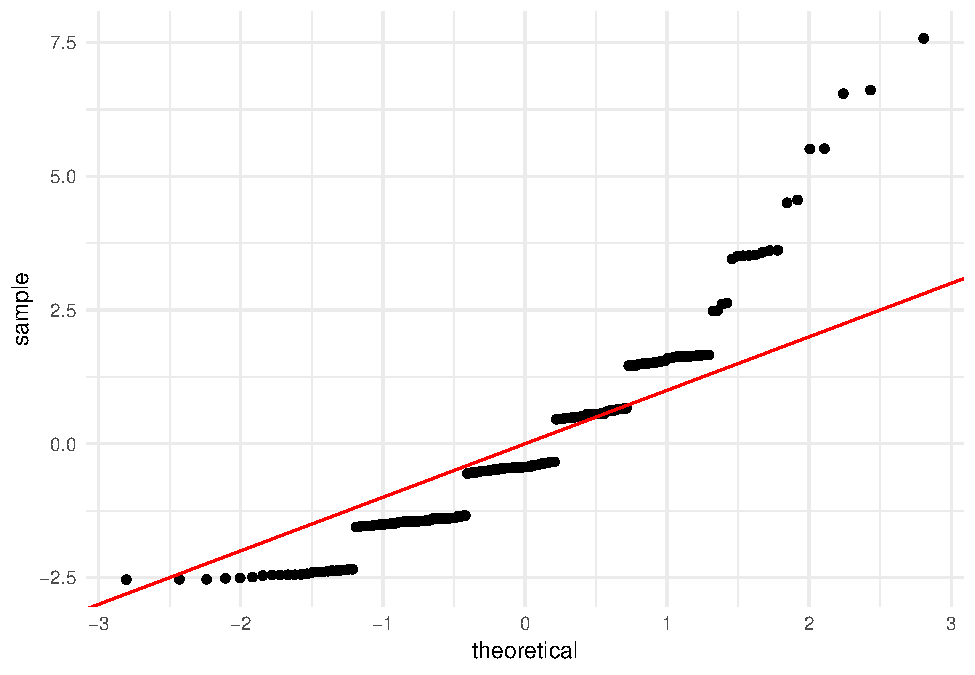
\includegraphics{Bayesian_statistics_files/figure-latex/unnamed-chunk-63-1.pdf}

A Binomial distributions has two parameters: \(p\) is the chance of
success and \(k\) is the number of attempts. \(p\) is a probability and
therefore can take values in the range from zero to one. With larger
\(p\) the distribution moves to the right. The mean of Binomial
distributions is the probability scaled by number of attempts,
\(M = kp\). Logically, there cannot be more successes then \(k\), but
with larger \(k\) the distribution gets wider. The variance is the odds
scaled by number of attempts, \(\textrm{Var} = kp(1-p)\). As mean and
variance depend on the exact same parameters, they cannot be set
independently. In fact, the relation \(Var = M(1-p)\) is parabolic, so
that variance is largest at \(p = .5\), but decreases towards both
boundaries. A Binomial distribution with, say \(k=10\) and \(p = .4\)
always has mean \(4\) and variance \(2.4\). This means, in turn, that an
outcome with a mean of \(4\) and a variance of \(3\) is not Binomially
distributed. This occurs frequently, when the success rate is not
identical across trials. A common solution is to use hierarchical
distributions, where the parameter \(p\) itself is distributed, rather
than fixed. A common distribution for \(p\) is the \emph{beta}
distribution and the \emph{logitnormal} distribution is an alternative.

The Binomial distribution has two boundaries, zero below and number of
attempts \(k\) above. While a lower boundary of zero is often natural,
one cannot always speak of a number of attempts. For example, the number
of times a customer returns to the car rental website does not yield a
natural interpretation of number of attempts. Rather, one could imagine
the situation as that any moment is an opportunity to hire a car. At the
same time, every single moment has a very, very small chance that a car
is hired, indeed. Under these conditions, an infinite (or painstakingly
large) number of opportunities and a very low rate, the random pattern
is neatly summarized by \emph{Poisson distributions}.

\subsubsection{Poisson distributions}\label{poisson_dist}

Some counting processes have no natural upper limit like the number of
trials in a test. In design research, a number of measures are such
\emph{unbounds counts}:

\begin{itemize}
\tightlist
\item
  number of erronous actions
\item
  frequency of returns
\item
  behavioural events, e.g.~showing explorative behaviour
\item
  physiological events, such as number of peaks in galvanic skin
  response
\end{itemize}

These measures can often be modelled as \emph{Poisson distributed}. A
useful way to think of unbound counts, is that they can happen at every
moment, but with a very small chance. Think of a longer interaction
sequence of a user with a system, where errors are recorded. It can be
conceived as an almost infinite number of opportunities to err, with a
very small chance of something to happen. The Poisson distribution is a
so called limiting case of the binomial distributions, with infinite
\(k\) and infinitely small \(p\). Of course, such a situation is
completely ideal. Yet, Poisson distributions fit such situations well
enough.

Poisson distributions possess only one parameter \(\lambda\) (lambda),
that is strictly positive and determines mean and variance of the
distribution alike: \(\lambda = M = \textrm{Var}\). As a matter of fact,
there cannot be massively dispersed distributions close to zero, nor
narrow ones in the far. Owing to the lower boundary, Poisson
distributions are \emph{asymmetric}, with the left tail always being
steeper. Higher \(\lambda\)s push the distribution away from the
boundary and the skew diminishes. It is commonly practiced to
approximate counts in the high numbers by \emph{normal distributions}.

\begin{Shaded}
\begin{Highlighting}[]
\NormalTok{mascutils}\OperatorTok{::}\KeywordTok{expand_grid}\NormalTok{(}\DataTypeTok{lambda =} \KeywordTok{c}\NormalTok{(}\DecValTok{2}\NormalTok{, }\DecValTok{4}\NormalTok{, }\DecValTok{8}\NormalTok{),}
                       \DataTypeTok{count =} \DecValTok{0}\OperatorTok{:}\DecValTok{20}\NormalTok{) }\OperatorTok
\StringTok{  }\KeywordTok{mutate}\NormalTok{(}\DataTypeTok{probability =} \KeywordTok{dpois}\NormalTok{(count, lambda)) }\OperatorTok\StringTok{ }
\StringTok{  }\KeywordTok{ggplot}\NormalTok{(}\KeywordTok{aes}\NormalTok{(}\DataTypeTok{x =}\NormalTok{ count, }\DataTypeTok{y =}\NormalTok{ probability)) }\OperatorTok{+}
\StringTok{  }\KeywordTok{geom_step}\NormalTok{() }\OperatorTok{+}
\StringTok{  }\KeywordTok{facet_grid}\NormalTok{(lambda}\OperatorTok{~}\NormalTok{.)}
\end{Highlighting}
\end{Shaded}

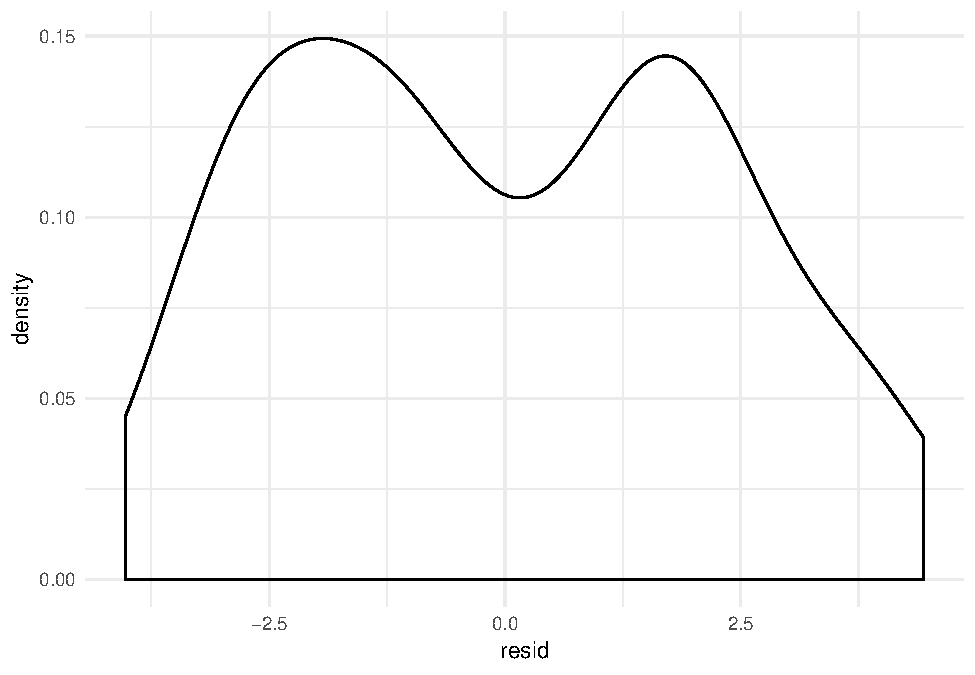
\includegraphics{Bayesian_statistics_files/figure-latex/unnamed-chunk-64-1.pdf}

The linkage between mean and variance is very strict. Only a certain
amount of randomness can be contained. If there is more randomness, and
that is almost certainly so, Poisson distributions are not appropriate.
One speaks of \emph{overdispersion} in such a case.

Consider a very simple video game, \emph{subway smurfer}, where the
player jumps and runs a little blue avatar on the roof of a train and
catches items passing by. Many items have been placed into the game, but
catching a single one is very difficult. The developers are aware that a
too low success rate would demotivate players as much as when the gane
is made to easy. In this experiment, only one player is recorded, and in
wonderful ways this player never suffers from fatigue, nor does he get
better with training. The player plays a 100 times and records the
catches after every run. In this idealized situation, the distribution
of catches would, indeed, follow a Poisson distribution, as in the
figure below.

Consider a variation of the experiment with 100 players doing one game
and less restrictive rules. Players come differently equipped to perform
visual search tasks and coordinate actions at high speeds. They are
tested at different times of the day and by chance feel a bit groggy or
energized. The chance of catching varies between players, which violates
the assumption that was borrowed from the Binomial, a constant chance
\(p\). The extra variation is seen in the wider of the two
distributions.

\begin{Shaded}
\begin{Highlighting}[]
\NormalTok{## }\AlertTok{FIXME}




\KeywordTok{data_frame}\NormalTok{(}\DataTypeTok{lambda =} \DecValTok{20}\NormalTok{,}
           \DataTypeTok{ci =} \KeywordTok{rpois}\NormalTok{(}\DecValTok{100}\NormalTok{, }\KeywordTok{log}\NormalTok{(lambda)),}
           \DataTypeTok{ci_ovdsp =} \KeywordTok{rpois}\NormalTok{(}\DecValTok{100}\NormalTok{, }\KeywordTok{log}\NormalTok{(lambda }\OperatorTok{+}\StringTok{ }\KeywordTok{rnorm}\NormalTok{(}\DecValTok{100}\NormalTok{, }\DecValTok{0}\NormalTok{, }\DecValTok{100}\NormalTok{)))}
\NormalTok{           ) }\OperatorTok\StringTok{ }
\StringTok{  }\KeywordTok{ggplot}\NormalTok{(}\KeywordTok{aes}\NormalTok{(}\DataTypeTok{x =}\NormalTok{ ci)) }\OperatorTok{+}
\StringTok{  }\KeywordTok{geom_histogram}\NormalTok{(}\KeywordTok{aes}\NormalTok{(}\DataTypeTok{fill =} \StringTok{"single participant"}\NormalTok{)) }\OperatorTok{+}
\StringTok{  }\KeywordTok{geom_histogram}\NormalTok{(}\KeywordTok{aes}\NormalTok{(}\DataTypeTok{x =}\NormalTok{ ci_ovdsp, }\DataTypeTok{fill =} \StringTok{"multi participants"}\NormalTok{), }\DataTypeTok{alpha =}\NormalTok{ .}\DecValTok{5}\NormalTok{) }\OperatorTok{+}
\StringTok{  }\KeywordTok{labs}\NormalTok{(}\DataTypeTok{fill=}\StringTok{"Count distributions"}\NormalTok{, }\DataTypeTok{x =} \StringTok{"outcome"}\NormalTok{, }\DataTypeTok{y =} \StringTok{"density"}\NormalTok{)}
\end{Highlighting}
\end{Shaded}

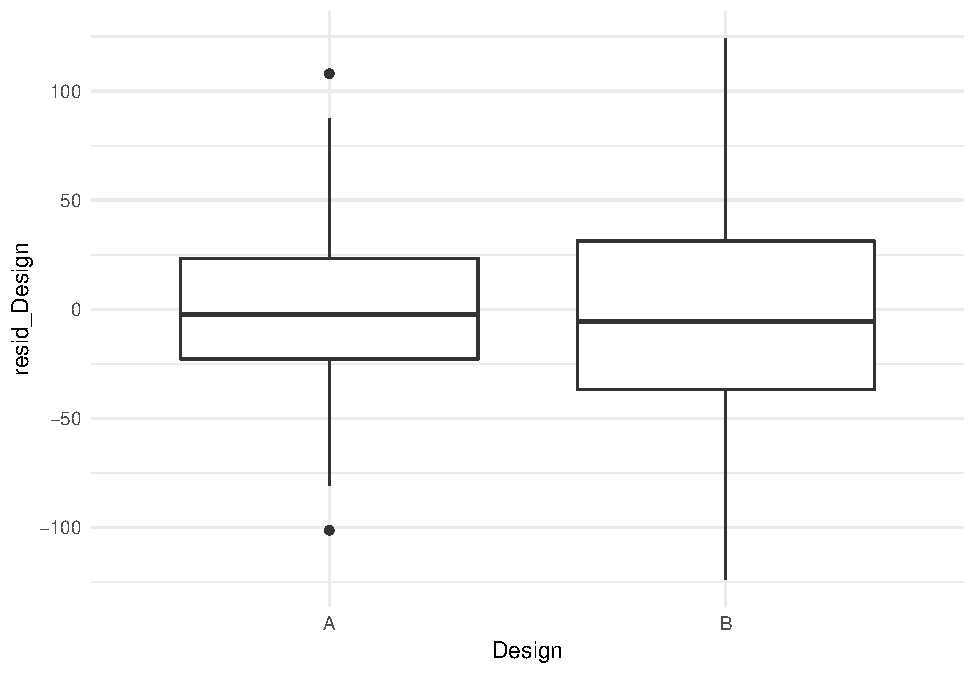
\includegraphics{Bayesian_statistics_files/figure-latex/unnamed-chunk-65-1.pdf}

Poisson distributions' lower boundary can cause trouble: the measure at
hand is truly required to include the lower bound. A person can perform
a sequence with no errors, catch zero items or have no friends on
facebook. But, you cannot complete an interaction sequence in zero steps
or have a conversation with less than two statements. Fortunately, once
a count measure has a lower boundary right of zero, the offset is often
available, such as the minimum necessary steps to complete a task. In
such a case, the number of errornous steps can be derived and used as a
measure, instead:

\[
\textrm{\#errors} = \textrm{\#steps} - \textrm{\#neccessary steps}
\]

Another lower bound problem arises, when there are hurdles. In traffic
research, the frequency of use public transport certainly is an
interesting variable. A straight-forward assessment would be to ask bus
passengers ``How many times have you taken the bus the last five
days?''. This clearly is a count measure, but it cannot be zero, because
the person is sitting in the bus right now. This could be solved by a
more inclusive form of inquiry, such as approaching random households.
But, the problem is deeper: actually, the whole population is of two
classes, those who use public transport and those who don't.

\subsubsection{Exponential distribution
{[}TBC{]}}\label{exponential-distribution-tbc}

Exponential distributions apply for measures of duration. Exponential
distributions have the same generating process as Poisson distributions,
except, that the \emph{duration for an event to happen} is the variable
of interest, rather than events in a given time. The same idealized
conditions of a completely unaffected subway smurfer player and constant
catchability of items, the duration between any two catches is
exponentially distributed. In more general, the chance for an event to
happen is the same at any moment, completely independent of how long one
has been waiting for it. For this property, the exponential distribution
is called \emph{memoryless}.

Durations are common measures in design research, most importantly,
time-on-task and reaction time. Unfortunately, the exponential
distribution is a poor approximation of the random pattern found in
duration measures. That is for two reasons: first, the exponential
distribution shares with Poisson, that it does not allow variance
between participants. Second, the distribution always starts at zero,
whereas human reactions always include some basic processing, and be
this just the velocity of signals passing nerve cells, which is far
below speed of sound (in air).

\subsubsection{Gamma distribution
{[}TBD{]}}\label{gamma-distribution-tbd}

\subsubsection{Normal distributions}\label{normal-distributions}

The best known distributions are \emph{normal distributions} or
\emph{Gaussian distributions}. These distributions arise mathematically
under the assumption of a myriad of small unrelated forces (SMURF)
pushing performance (or any other outcome) up or down. As SMURFs work in
all directions independently, their effects often average out and the
majority of observations stays clumped together in the center, more or
less.

Normal distributions have two parameters: \(\mu\) marks the center and
mean of the distribution. The linear models introduced later are aiming
at predicting \(\mu\). The second parameter \(\sigma\) represents the
dispersion of the random pattern. When randomness is pronounced, the
center of the distribution gets less mass assigned, as the tails get
wider.

Different to Poisson and Binomial distributions, mean and variance of
the distribution can be set independently and overdispersion is never an
issue.

\begin{Shaded}
\begin{Highlighting}[]
\KeywordTok{ggplot}\NormalTok{(}\KeywordTok{data.frame}\NormalTok{(}\DataTypeTok{x =} \KeywordTok{c}\NormalTok{(}\OperatorTok{-}\DecValTok{4}\NormalTok{, }\DecValTok{4}\NormalTok{)), }\KeywordTok{aes}\NormalTok{(}\DataTypeTok{x =}\NormalTok{ x)) }\OperatorTok{+}
\StringTok{  }\KeywordTok{stat_function}\NormalTok{(}\DataTypeTok{fun =}\NormalTok{ dnorm, }\DataTypeTok{args =} \KeywordTok{list}\NormalTok{(}\DataTypeTok{mean =} \DecValTok{0}\NormalTok{, }\DataTypeTok{sd =} \DecValTok{1}\NormalTok{), }\DataTypeTok{mapping =} \KeywordTok{aes}\NormalTok{(}\DataTypeTok{colour =} \StringTok{"Normal( 0, 1)"}\NormalTok{)) }\OperatorTok{+}
\StringTok{  }\KeywordTok{stat_function}\NormalTok{(}\DataTypeTok{fun =}\NormalTok{ dnorm, }\DataTypeTok{args =} \KeywordTok{list}\NormalTok{(}\DataTypeTok{mean =} \OperatorTok{-}\FloatTok{1.5}\NormalTok{, }\DataTypeTok{sd =} \FloatTok{0.5}\NormalTok{), }\DataTypeTok{mapping =} \KeywordTok{aes}\NormalTok{(}\DataTypeTok{colour =} \StringTok{"Normal(-1.5, 0.5)"}\NormalTok{)) }\OperatorTok{+}
\StringTok{  }\KeywordTok{stat_function}\NormalTok{(}\DataTypeTok{fun =}\NormalTok{ dnorm, }\DataTypeTok{args =} \KeywordTok{list}\NormalTok{(}\DataTypeTok{mean =} \FloatTok{0.5}\NormalTok{, }\DataTypeTok{sd =} \DecValTok{2}\NormalTok{), }\DataTypeTok{mapping =} \KeywordTok{aes}\NormalTok{(}\DataTypeTok{colour =} \StringTok{"Normal(0.5,1.5)"}\NormalTok{)) }\OperatorTok{+}
\StringTok{  }\KeywordTok{labs}\NormalTok{(}\DataTypeTok{colour=}\StringTok{"Normal distributions"}\NormalTok{, }\DataTypeTok{x =} \StringTok{"outcome"}\NormalTok{, }\DataTypeTok{y =} \StringTok{"density"}\NormalTok{)}
\end{Highlighting}
\end{Shaded}

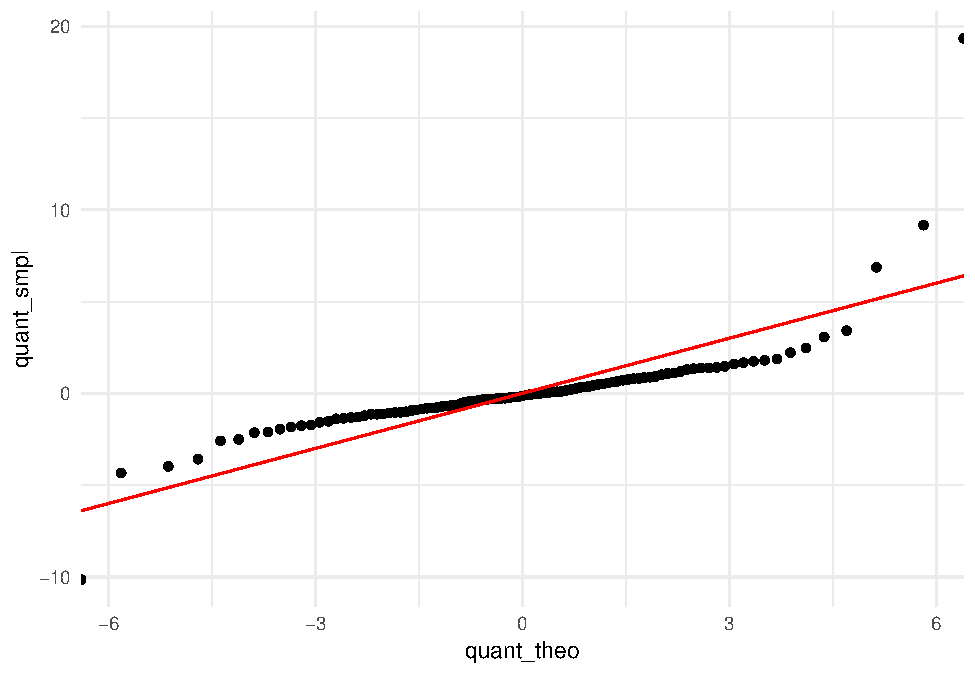
\includegraphics{Bayesian_statistics_files/figure-latex/unnamed-chunk-68-1.pdf}

Normal distributions have the compelling interpretation of summarizing
the effect of SMURFs. They serve to capture randomness in a broad class
of regression models and other statistical approaches. The problem with
normal distributions is that they only capture the pattern of randomness
under two assumption. The first assumption is that the outcome is
continuous. While that holds for duration as a measure of performance,
it would not hold for counting the errors a user makes. The second
assumption is that the SMURFs are truly additive, like the forces add
up, when two pool balls collide. This appears subtle at first, but it
has the far reaching consequence that the outcome variable must have an
infinite range in both directions, which is impossible.

The normal distribution is called ``normal'', because people normally
use it. Of course not. It gots its name for a deeper reason, commonly
known (and held with awe) as the \emph{central limit theorem}.
Basically, this theorem proves what we have passingly observed at
binomial and Poisson distributions: the more they move to the right, the
more symmetric they get. The central limit theorem proves that, in the
long run, a wide range of distributions are indistinguishable from the
normal distribution. In practice, infinity is relative. In some cases,
it is reasonable to trade in some fidelity for convenience and good
approximations make effective statisticians. As a general rule, the
normal distribution approximates other distributions well, when the
majority of measures stay far from the natural boundaries. That is the
case in experiments with very many attempts and moderate
chances(e.g.~signal detection experiments), when counts are in the high
numbers (number of clicks in a complex task) or with long durations.
However, these rules are no guarantee and careful model criticism is
essential.

Measurement is prime and specialized (non-central-limit) distributions
remain the first recommendation for capturing measurement errors. The
true salvation of normal distributions is their application in
\emph{multi-level models}. While last century statistics was reigned by
questions of location, and variance considered nuisance, new statistics
care for variation. Most notably, amount of variation in a population is
added as a central idea in multi-level modelling, which is commonly
referred to as \emph{random effects}. These models can become highly
complex and convenience is needed more than ever. Normal distributions
tie things together in multi-level models, as they keep location and
dispersion apart, tidy.

The dilemma is then solved with the introduction of \emph{generalized
linear models}, which is a framework for using linear models with
appropriate error distributions. Fortunately, MLM and GLM work
seemlessly together. With MLM we can conveniently build graceful
likelihood models, using normal distributions for populations. The GLM
part is a thin layer to get the measurement scale right and choose the
right error distribution, just like a looking glass.

\subsubsection{t distribution {[}TBD{]}}\label{t-distribution-tbd}

\subsubsection{Exercises:}\label{exercises}

\begin{enumerate}
\def\labelenumi{\arabic{enumi}.}
\tightlist
\item
  Google it: speed of sound and signal velocity in nerve cells.
\end{enumerate}

\section{Bayesian estimation}\label{bayesian-estimation}

Frequentist statistics falls short on recognizing that research is
incremental. Bayesian statistics embraces the idea of gradually increase
in certainty. Why has it not been adopted earlier? The reason is it was
unfeasible. The innocent multiplication of prior and likelihood is a
complex integral, which in most cases has no analytic solution. If you
have enjoyed a classic statistics education, you may remember that the
computation of sum of squares (explained and residual) can be done by
paper and pencil in reasonable time. And that is precisely how
statistical computations has been performed before the advent of
electronic computing machinery. In the frequentist statistical framework
(some call it a zoo), ingenious mathematicians have developed procedures
that were rather easy to compute. That made statistical data analysis
possible in those times. It came at costs, though:

\begin{enumerate}
\def\labelenumi{\arabic{enumi}.}
\tightlist
\item
  procedures make more or less strong assumptions, limiting their
  applicability. Procedures become islands.
\item
  procedures are asymptotically accurate with inference being accurate
  at large sample sizes only
\item
  common researchers do not understand crucial elements, for example
  deriving the F distribution
\end{enumerate}

Expensive computation is in the past. Modern computers can simulate
realistic worlds in real time and the complex integrals in Bayesian
statistics they solve hands down. When analytical solutions do not
exist, the integrals can still be solved using numerical procedures.
Numerical procedures have been used in frequentist statistics, too, for
example the iterative least squares algorithm applies for Generalized
Linear Models, or the Newton-Rapson optimizer can be used to find the
maximum likelihood estimate. However, these procedures are too limited
as they fail for highly multidimensional problems as they are common in
Linear Mixed-Effects Models. Moreover, they do not allow to approximate
integrals.

Most Bayesian estimation engines these days ground on a numerical
procedure called Markov-Chain Monte-Carlo sampling. The method differs
from the earlier mentioned in that it basically is a random number
generator. The basic MCMC algorithm is so simple, it can be explained on
half a page and implemented with 25 lines of code. Despite its
simplicity, the MCMC algorithm is applicable to practically all
statistical problems one can imagine. Being so simple and generic at the
same time must come at some costs. The downside of MCMC sampling still
is computing time. Models with little data and few variables, like the
rainfall case above, are estimated within a few minutes. Linear-mixed
effects models, which we will encounter later in this book, can take
hours and large psychometric models (which are beyond the scope), can
take up to a few days.

Still, the MCMC algorithm not only delivers some accurate point
estimates, it produces the full posterior distribution. This lets us
characterize a parameters magnitude and degree of (un)certainty. Let's
run an analysis on the 20 rainfall observations to see how this happens.

\begin{Shaded}
\begin{Highlighting}[]
\KeywordTok{attach}\NormalTok{(Rainfall)}
\end{Highlighting}
\end{Shaded}

\begin{Shaded}
\begin{Highlighting}[]
\NormalTok{M_}\DecValTok{1}\NormalTok{ <-}\StringTok{ }
\StringTok{  }\NormalTok{Rain }\OperatorTok
\StringTok{  }\KeywordTok{stan_glm}\NormalTok{(rain }\OperatorTok{~}\StringTok{ }\NormalTok{cloudy }\OperatorTok{-}\DecValTok{1}\NormalTok{, }
           \DataTypeTok{family =}\NormalTok{ binomial,}
           \DataTypeTok{data =}\NormalTok{ .)}
\end{Highlighting}
\end{Shaded}

What the estimation does, is to calculate the \emph{posterior
distribution} from the observations. The \emph{posterior distribution}
contains the probability (more precisely: the \emph{density}) for all
possible values of the parameter in question. The following density plot
represents our belief about the parameter \(P(rain|cloudy)\) after we
have observed twenty days:

\begin{Shaded}
\begin{Highlighting}[]
\KeywordTok{posterior}\NormalTok{(M_}\DecValTok{1}\NormalTok{) }\OperatorTok
\StringTok{  }\KeywordTok{filter}\NormalTok{(type }\OperatorTok{==}\StringTok{ "fixef"}\NormalTok{) }\OperatorTok\StringTok{ }
\StringTok{  }\KeywordTok{mutate}\NormalTok{(}\DataTypeTok{chance_of_rain =} \KeywordTok{plogis}\NormalTok{(value)) }\OperatorTok\StringTok{ }
\StringTok{  }\KeywordTok{ggplot}\NormalTok{(}\KeywordTok{aes}\NormalTok{(}\DataTypeTok{x =}\NormalTok{ chance_of_rain, }\DataTypeTok{fill =}\NormalTok{ parameter, }\DataTypeTok{col =}\NormalTok{ parameter)) }\OperatorTok{+}
\StringTok{  }\KeywordTok{geom_density}\NormalTok{(}\DataTypeTok{alpha =}\NormalTok{ .}\DecValTok{5}\NormalTok{)}
\end{Highlighting}
\end{Shaded}

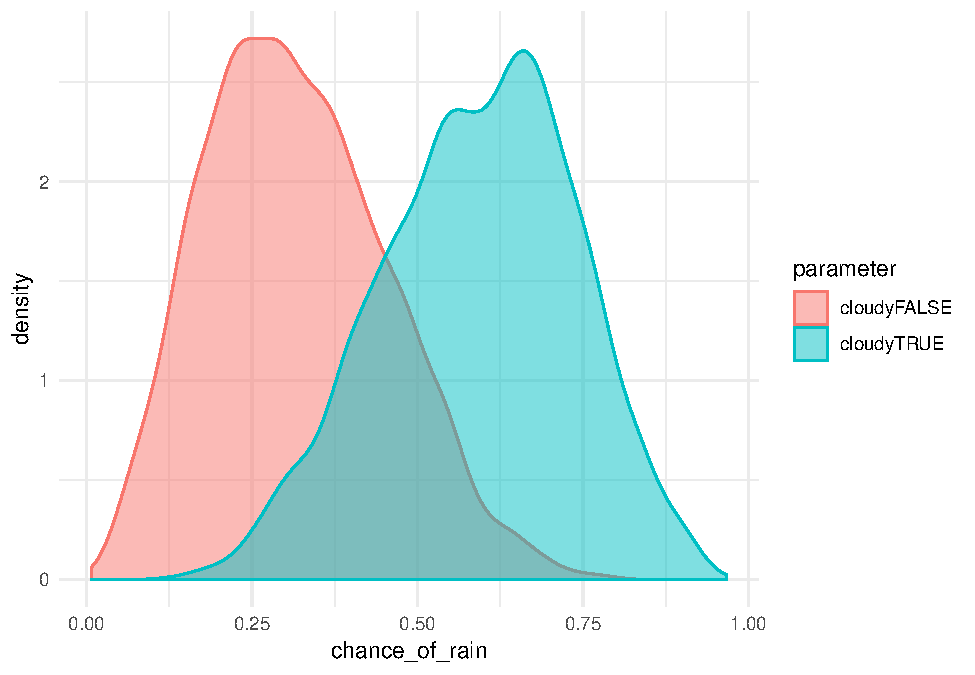
\includegraphics{Bayesian_statistics_files/figure-latex/umbrella_post-1.pdf}

\begin{Shaded}
\begin{Highlighting}[]
\KeywordTok{detach}\NormalTok{(Rainfall)}
\end{Highlighting}
\end{Shaded}

From the posterior distribution, we can deduct all kinds of summary
statistics, such as:

\begin{enumerate}
\def\labelenumi{\arabic{enumi}.}
\tightlist
\item
  the most likely value for a parameter in question is called the
  \emph{posterior mode} and is the same as the \emph{maximum likelihood
  estimate} when prior knowledge is absent.
\item
  the average of parameter values, weighted by their probability is
  called the \emph{posterior mean}
\item
  a defined range to express 95\% (or any other level of) certainty is
  the \emph{95\% credibility interval}
\end{enumerate}

We can also make non-standard evaluations on the posterior distribution,
for example: How certain is it that \(P(rain|cloudy) < 0.7\)? We'll
demonstrate the use of this in the next section.

Coming back to MCMC: how is this distribution actually produced. In
plain words, MCMC makes a random walk through parameter space. Regions
where the true value is more likely to be are just visited more often.
The posterior distribution plots above are actually just frequency
plots.

{[}ILLUSTRATE RANDOM WALK{]}

\section{What is wrong with classic statistics?
{[}TBC{]}}\label{what-is-wrong-with-classic-statistics-tbc}

The p-value {[}\ldots{}{]} Imagine giant replication study that showed
that 35\% of published psychology studies are not replicable. In fact,
such a study exists and it has far-reaching consequences. {[}\ldots{}{]}
{[}REF{]} shows that rejection bias is one reason: studies that have not
reached the \emph{magic .05 level} of significance, have a lower chance
of publication. {[}REF{]} sees as a reason that author's implicitly
trick the system by \emph{the garden of forking paths} strategy. The
research project collects an array of variables, followed by a fishing
expediture. Theory is conventiently considered last, but written up in a
pseudo-a prior way.

\chapter{Getting started with R}\label{getting_started_r}

In this book, we will be using the statistical computing environment R.
R at its core is a programming language that specializes on statistics
and data analysis. Like all modern programming languages, R is more than
just a compiler or interpreter that translates human-writeable formal
statements into something a computer understands and can execute. R
comes with a complete set of standard libraries that cover the usual
basic stuff, as well as a collection of common statistical routines, for
example the t-test or functions to compute mean and variance. Even
regression analysis and plotting is included in R. Finally, packaged
with R comes a rudimentary programming environment, including a console,
a simple editor and a help system.

Most of what comes packaged with R, we will set aside. R is basically a
brilliantly designed programming language for the task, but many of the
standard libraries are an inconsistent and outdated mess. For example, R
comes with a set of commands to import data from various formats (SPSS,
CSV, etc.). Some of these commands produce objects called data.frames,
whereas others return lists of lists. Although one can convert lists
into dataframes, it is easier and prevents confusion if all import
functions simply create dataframes. As another example, to sort a data
frame by participant number, one has to write the following syntax soup:

\texttt{D{[}order(D\$Part),{]}}

In the past few years, a single person, Hadley Wickham, has almost
single-handedly started an initiative known as the \emph{tidyverse}. The
tidyverse is a growing collection of libraries that ground on a coherent
and powerful set of principles for data management. One of the core
packages is \emph{dplyr} and it introduces a rich, yet rather generic,
set of commands for data manipulation. The sorting of a data frame
mentioned above would be written as

\texttt{D\ \%\textgreater{}\%\ arrange(Part)}

One of Wickham's first and well-known contributions is the \emph{ggplot}
system for graphics. Think of R's legacy graphics system as a zoo of
individual routines, one for boxplots, another one for scatterplots asf.
Like animals in a zoo, they live in different habitats with practically
no interaction. ggplot implements a rather abstract framework for data
plots, where all pieces can be combined in a myriad of ways, using a
simple and consistent syntax.

Where to get these gems? R is an open source system and has spawned an
open ecosystem for statistical computing. Thousands of extensions for R
have been made available by data scientists for data scientists. The
majority of these packages is available through the \emph{comprehensive
R archive network (CRAN)}. For the common user it suffices to think of
CRAN as an internet catalogue of packages, that can be searched and
where desired packages can be downloaded and installed in an instance.

Finally, R comes with a very rudimentary programming environment that
carries the questionable charm of early 1990s. Whereas several
alternatives exist, most R users will feel most comfortable with the R
programming environment Rstudio. At the time of writing, it is the most
user-friendly and feature rich software to program in R. The next
sections describe how you can set up a fully functional environment and
verify that it works. Subsequently, we will get to know the basics of
programming in R.

\section{Setting up the R
environment}\label{setting-up-the-r-environment}

First, we make sure that you have R and Rstudio downloaded and installed
on your computer. The two programs can be retrieved from the addresses
below. Make sure to select the version fit for your operating system.

\begin{itemize}
\tightlist
\item
  \href{http://www.r-project.org}{R}
\item
  \href{http://www.rstudio.com}{Rstudio}
\end{itemize}

If you fully own the computer you are working with, meaning that you
have administrator rights, just do the usual downloading and running of
the setup. If everything is fine, you'll find R and Rstudio installed
under \texttt{c\textbackslash{}Programs\textbackslash{}} and both are in
your computers start menu. You can directly proceed to the installation
of packages.

In corporate environments, two issues can arise with the installation:
first a user may not have administrator rights to install programs to
the common path \texttt{c:\textbackslash{}programs\textbackslash{}}.
Second, the home directory may reside on a network drive, which is
likely to cause trouble when installing packages.

If you have no administrator rights, you must choose your home directory
during the setup. If that is a local directory,
(\texttt{c:/Users/YourName/}), this should work fine and you can proceed
with the installation of packages.

If your home directory (i.e. \texttt{My\ Documents}) is located on a
network drive, this is likely to cause trouble. In such a case, you must
install R and Rstudio to a local directory (on your computers hard
drive), where you have full read/write access. In the following, it is
assumed that this directory is \texttt{D:/Users/YourName/}:

\begin{enumerate}
\def\labelenumi{\arabic{enumi}.}
\tightlist
\item
  create a directory \texttt{D:/Users/YourName/R/}. This is where both
  programs, as well as packages will reside.
\item
  create a sub directory \texttt{Rlibrary} where all additional packages
  reside (R comes with a pack of standard packages, which are in a
  read-only system directory).
\item
  start Rstudio
\item
  create a regular text file
  \texttt{File\ -\textgreater{}\ New\ File\ -\textgreater{}\ Text\ file}
\item
  copy and paste code from the box below
\item
  save the file as \texttt{.Rprofile} in \texttt{D:/Users/YourName/R/}
\item
  open the menu and go to
  \texttt{Tools\ -\textgreater{}\ Global\ options\ -\textgreater{}\ General\ -\textgreater{}\ Default\ working\ directory}.
  Select \texttt{D:/Users/YourName/R/}.
\end{enumerate}

\begin{Shaded}
\begin{Highlighting}[]
\NormalTok{## .Rprofile}

\KeywordTok{options}\NormalTok{(}\DataTypeTok{stringsAsFactors =} \OtherTok{FALSE}\NormalTok{)}

\NormalTok{.First <-}\StringTok{ }\ControlFlowTok{function}\NormalTok{()\{}
\NormalTok{  RHOME <<-}\StringTok{ }\KeywordTok{getwd}\NormalTok{()}
    \KeywordTok{cat}\NormalTok{(}\StringTok{"}\CharTok{\textbackslash{}n}\StringTok{Loading .Rprofile in"}\NormalTok{, }\KeywordTok{getwd}\NormalTok{(), }\StringTok{"}\CharTok{\textbackslash{}n}\StringTok{"}\NormalTok{)}
  \KeywordTok{.libPaths}\NormalTok{(}\KeywordTok{c}\NormalTok{(}\KeywordTok{paste0}\NormalTok{(RHOME,}\StringTok{"Rlibrary"}\NormalTok{), }\KeywordTok{.libPaths}\NormalTok{()))}
\NormalTok{\}}

\NormalTok{.Last <-}\StringTok{ }\ControlFlowTok{function}\NormalTok{()\{ }
  \KeywordTok{cat}\NormalTok{(}\StringTok{"}\CharTok{\textbackslash{}n}\StringTok{Goodbye at "}\NormalTok{, }\KeywordTok{date}\NormalTok{(), }\StringTok{"}\CharTok{\textbackslash{}n}\StringTok{"}\NormalTok{)}
\NormalTok{\}}
\end{Highlighting}
\end{Shaded}

With the above steps you have created a customized start-up profile for
R. The profile primarily sets the library path to point to a directory
on the computers drive. As you are owning this directory, R can install
the packages without admin rights. In the second part, you configure
Rstudio's default path, which is where R, invoked from Rstudio, searches
for the .Rprofile.

After closing and reopening Rstudio, you should see a message in the
console window saying:

\begin{quote}
Loading .Rprofile in D:/Users/YourName/R/
\end{quote}

That means that R has found the \texttt{.Rprofile} file and loaded it at
start-up. The \texttt{.Rprofile} file primarily sets the path of the
\emph{library}, which is the collection of packages you install
yourself. Whether this was successful can be checked by entering the
\texttt{console} window in Rstudio, type the command below and hit
Enter.

\begin{Shaded}
\begin{Highlighting}[]
\KeywordTok{.libPaths}\NormalTok{()}
\end{Highlighting}
\end{Shaded}

If your installation went fine, you should see an output like the
following. If the output lacks the first entry, your installation was
not successful and you need to check all the above steps.

\begin{quote}
{[}1{]} ``D:/Users/YourName/R/Rlibrary'' ``C:/Program
Files/R/R-3.3.0/library''
\end{quote}

\subsection{Installing CRAN packages}\label{installing-cran-packages}

While R comes with a set of standard packages, thousands of packages are
available to enhance functionality for every purpose you can think of.
Most packages are available from the \emph{Comprehensive R Network
Archive (CRAN)}.

For example, the package \emph{foreign} is delivered with R and provides
functions to read data files in various formats, e.g.~SPSS files. The
package \emph{haven} is a rather new package, with enhanced
functionality and usability. It is not delivered with R, hence, so we
have to fetch it.

Generally, packages need to be \emph{installed once} on your system and
to be \emph{loaded everytime} you need them. Installation is fairly
straight-forward once your R environment has been setup correctly and
you have an internet connection.

In this book we will use a number of additional packages from CRAN. The
listed packages below are all required packages, all can be loaded using
the \texttt{library(package)} command. The package \emph{tidyverse} is a
metapackage that installs and loads a number of modern packages. The
ones being used in this book are:

\begin{itemize}
\tightlist
\item
  \emph{dplyr} and \emph{tidyr} for data manipulation
\item
  \emph{ggplot} for graphics
\item
  \emph{haven} for reading and writing files from other statistical
  packages
\item
  \emph{readr} for reading and writing text-based data files (e.g., CSV)
\item
  \emph{readxl} for reading Excel files
\item
  \emph{stringr} for string matching and manipulation
\end{itemize}

\begin{Shaded}
\begin{Highlighting}[]
\NormalTok{## tidyverse}
\KeywordTok{library}\NormalTok{(tidyverse)}

\NormalTok{## data manipulation}
\KeywordTok{library}\NormalTok{(openxlsx)}

\NormalTok{## plotting}
\KeywordTok{library}\NormalTok{(gridExtra)}

\NormalTok{## regression models}
\KeywordTok{library}\NormalTok{(rstanarm)}

\NormalTok{## other}
\KeywordTok{library}\NormalTok{(devtools) ## only needed for installing from Github}
\KeywordTok{library}\NormalTok{(knitr)}

\NormalTok{## non-CRAN packages}
\KeywordTok{library}\NormalTok{(mascutils)}
\KeywordTok{library}\NormalTok{(bayr)}
\end{Highlighting}
\end{Shaded}

We start by \emph{checking the packages}:

\begin{enumerate}
\def\labelenumi{\arabic{enumi}.}
\tightlist
\item
  create a new R file by
  \texttt{File\ -\/-\textgreater{}\ New\ file\ -\/-\textgreater{}\ R\ script}
\item
  copy and paste the above code to that file and run it. By repeatedly
  pressing \texttt{Ctrl-Return} you run every line one-by-one. As a
  first time user with a fresh installation, you will now see error
  messages like:
\end{enumerate}

\begin{quote}
Error in library(tidyverse) : there is no package called `tidyverse'
\end{quote}

This means that the respective package is not yet present in your R
library. Before you can use the package \emph{tidyverse} you have to
install it from CRAN. For doing so, use the built-in package management
in RStudio, which fetches the package from the web and is to be found in
the tab \emph{Packages}. At the first time, you may have to select a
repository and refresh the package list, before you can find and install
packages. Then click \texttt{Install}, enter the names of the missing
package(s) and install. On the R console the following command downloads
and installs the package \emph{tidyverse}.

\begin{Shaded}
\begin{Highlighting}[]
\KeywordTok{install.packages}\NormalTok{(}\StringTok{"tidyverse"}\NormalTok{)}
\end{Highlighting}
\end{Shaded}

CRAN is like a giant stream of software pebbles, shaped over time in a
growing tide. Typically, a package gets better with every version, be it
in reliability or versatility, so you want to be up-to-date. Rstudio has
a nice dialogue to update packages and there is the R command:

\begin{Shaded}
\begin{Highlighting}[]
\KeywordTok{update.packages}\NormalTok{(}\StringTok{"tidyverse"}\NormalTok{)}
\end{Highlighting}
\end{Shaded}

Finally, run the complete code block at once by selecting it and
\texttt{Ctrl-Enter}. You will see some output to the console, which you
should check once again. Unless the output contains any error messages
(like above), you have successfully installed and loaded all packages.

\emph{Note} that R has a somewhat idiosyncratic jargon: many languages,
such as Java or Python, call ``libraries'' what R calls ``packages''.
\emph{The} library in R is strictly the set of packages installed on
your computer and the \texttt{library} command loads a package from the
library.

\subsection{Installing packages from
Github}\label{installing-packages-from-github}

Two packages, \emph{mascutils} and \emph{bayr} are written by the author
of this book. They have not yet been committed to CRAN, but they are
available on \emph{Github} which is a general purpose versioning system
for software developers and few authors. Fortunately, with the help of
the \emph{devtools} package it is rather easy to install these packages,
too. Just enter the Rstudio console and type:

\begin{Shaded}
\begin{Highlighting}[]
\KeywordTok{library}\NormalTok{(devtools)}
\KeywordTok{install_github}\NormalTok{(}\StringTok{"schmettow/mascutils"}\NormalTok{)}
\KeywordTok{install_github}\NormalTok{(}\StringTok{"schmettow/bayr"}\NormalTok{)}
\end{Highlighting}
\end{Shaded}

Again, you have to do that only once after installing R and you can
afterwards load the packages with the \texttt{library} command. Only if
the package gets an update to add functionality or remove bugs, you need
to run these commands again.

\subsection{A first statistical program}\label{first_program}

After you have set up your R environment, you are ready to run your
first R program (you will not yet understand all the code, but as you
proceed with this book, all will become clear):

\begin{enumerate}
\def\labelenumi{\arabic{enumi}.}
\tightlist
\item
  Stay in the file where you have inserted and run the above code for
  loading the packages.
\item
  Find the \emph{environment tab} in Rstudio. It should be empty.
\item
  Copy-and-paste the code below into your first file, right after
  library commands.
\item
  Run the code lines one-by-one and observe what happens (in RStudio:
  Ctrl-Enter)
\end{enumerate}

\begin{Shaded}
\begin{Highlighting}[]
\NormalTok{## Simulation of a data set with 100 participants }
\NormalTok{## in two between-subject conditions}
\NormalTok{N <-}\StringTok{ }\DecValTok{100}
\NormalTok{levels <-}\StringTok{ }\KeywordTok{c}\NormalTok{(}\StringTok{"control"}\NormalTok{,}\StringTok{"experimental"}\NormalTok{)}
\NormalTok{Group <-}\StringTok{ }\KeywordTok{rep}\NormalTok{(levels, N}\OperatorTok{/}\DecValTok{2}\NormalTok{)}
\NormalTok{age <-}\StringTok{ }\KeywordTok{round}\NormalTok{(}\KeywordTok{runif}\NormalTok{(N, }\DecValTok{18}\NormalTok{, }\DecValTok{35}\NormalTok{),}\DecValTok{0}\NormalTok{)}
\NormalTok{outcome <-}\StringTok{ }\KeywordTok{rnorm}\NormalTok{(N, }\DecValTok{42} \OperatorTok{*}\StringTok{ }\DecValTok{5}\NormalTok{, }\DecValTok{10}\NormalTok{) }\OperatorTok{+}\StringTok{ }\NormalTok{(Group }\OperatorTok{==}\StringTok{ "experimental"}\NormalTok{) }\OperatorTok{*}\StringTok{ }\DecValTok{42}
\NormalTok{Experiment <-}\StringTok{ }\KeywordTok{data_frame}\NormalTok{(Group, age, outcome)}

\NormalTok{Experiment }\OperatorTok\StringTok{ }\KeywordTok{sample_n}\NormalTok{(}\DecValTok{8}\NormalTok{)}
\end{Highlighting}
\end{Shaded}

\begin{tabular}{l|r|r}
\hline
Group & age & outcome\\
\hline
control & 30 & 197\\
\hline
control & 31 & 190\\
\hline
control & 30 & 206\\
\hline
control & 29 & 210\\
\hline
experimental & 20 & 238\\
\hline
control & 30 & 216\\
\hline
experimental & 20 & 256\\
\hline
control & 34 & 215\\
\hline
\end{tabular}

\begin{Shaded}
\begin{Highlighting}[]
\NormalTok{## Plotting the distribution of outcome}
\NormalTok{Experiment }\OperatorTok\StringTok{ }
\StringTok{  }\KeywordTok{ggplot}\NormalTok{( }\KeywordTok{aes}\NormalTok{(}\DataTypeTok{x =}\NormalTok{ outcome) ) }\OperatorTok{+}\StringTok{ }
\StringTok{  }\KeywordTok{geom_density}\NormalTok{(}\DataTypeTok{fill =} \DecValTok{1}\NormalTok{)}
\end{Highlighting}
\end{Shaded}

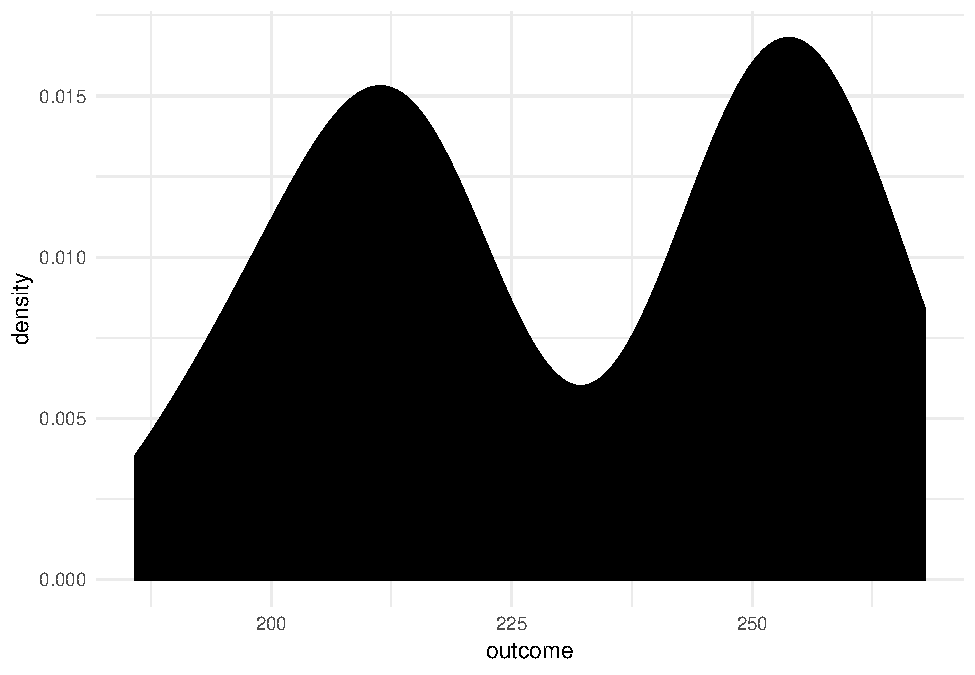
\includegraphics{Getting_started_with_R_files/figure-latex/first_simulation_1-1.pdf}

\begin{Shaded}
\begin{Highlighting}[]
\NormalTok{## ... outcome by group}
\NormalTok{Experiment }\OperatorTok\StringTok{ }
\StringTok{  }\KeywordTok{ggplot}\NormalTok{( }\KeywordTok{aes}\NormalTok{(}\DataTypeTok{fill =}\NormalTok{ Group, }\DataTypeTok{x =}\NormalTok{ outcome) ) }\OperatorTok{+}\StringTok{ }
\StringTok{  }\KeywordTok{geom_density}\NormalTok{()}
\end{Highlighting}
\end{Shaded}

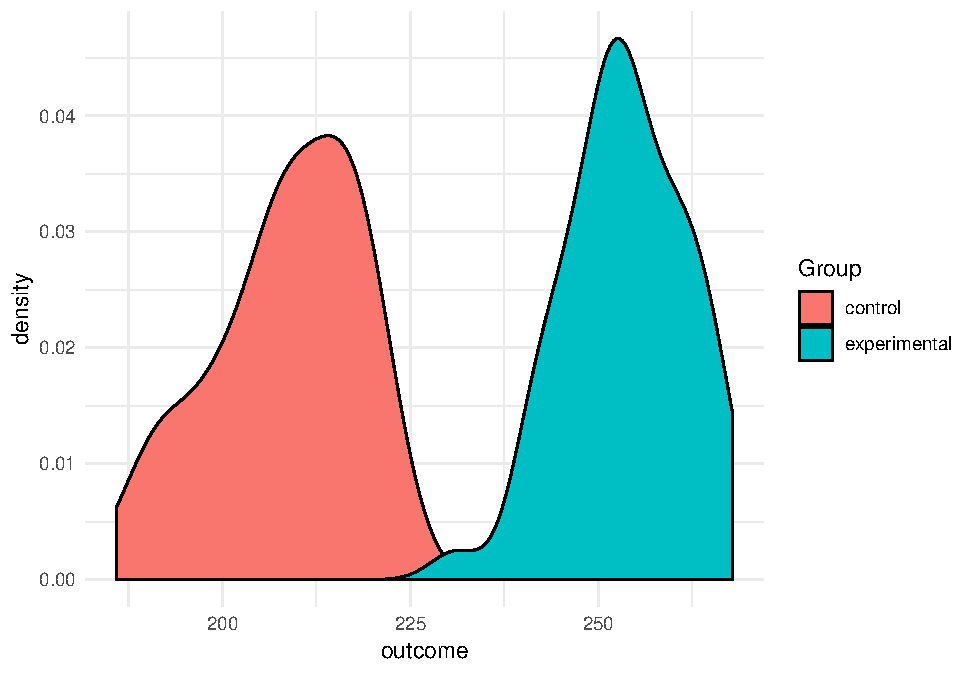
\includegraphics{Getting_started_with_R_files/figure-latex/first_simulation_1-2.pdf}

\begin{Shaded}
\begin{Highlighting}[]
\NormalTok{## ... statistical model comparing the groups}

\NormalTok{model <-}\StringTok{ }\KeywordTok{stan_glm}\NormalTok{(}\DataTypeTok{formula =}\NormalTok{ outcome }\OperatorTok{~}\StringTok{ }\NormalTok{Group, }
            \DataTypeTok{data =}\NormalTok{ Experiment) }
\end{Highlighting}
\end{Shaded}

\begin{Shaded}
\begin{Highlighting}[]
\KeywordTok{fixef}\NormalTok{(model)}
\end{Highlighting}
\end{Shaded}

\begin{longtable}[]{@{}lrrr@{}}
\toprule
fixef & center & lower & upper\tabularnewline
\midrule
\endhead
Intercept & 211.9 & 209.1 & 214.7\tabularnewline
Groupexperimental & 38.5 & 34.6 & 42.3\tabularnewline
\bottomrule
\end{longtable}

Observe Console, Environment and Plots. Did you see

\begin{itemize}
\tightlist
\item
  how the \emph{Environment} window is populated with new variables
  (Values and Data)?
\item
  a table appears in the \emph{Console}, when executing the
  \texttt{summary(Experiment)} command?
\item
  how the ``camel-against-the-light'' in \emph{Plots} tab morphed into
  ``two-piles-of-colored-sugar''?
\end{itemize}

Congratulations! You have just

\begin{itemize}
\tightlist
\item
  simulated data of a virtual experiment with two groups
\item
  summarized the data
\item
  plotted the data and
\item
  estimated a Bayesian regression model that compares the two groups.
\end{itemize}

Isn't it amazing, that in less than 20 simple statements we have just
reached the level of a second-year bachelor student? Still, you may find
the R output a little inconvenient, as you may want to save the output
of your data analysis. Not long ago, that really was an issue, but in
the past few years R has become a great tool for \emph{reproducable
research}. The most simple procedure of saving your analysis for print
or sharing is to:

\begin{enumerate}
\def\labelenumi{\arabic{enumi}.}
\tightlist
\item
  save the R file your have created by hitting \texttt{CTRL-S} and
  selecting a directory and name.
\item
  in RStudio open \texttt{File\ -\/-\textgreater{}\ Compile\ notebook}
  and select Word as a format.
\item
  Hit \texttt{Compile}
\end{enumerate}

A new Word document should appear that shows all code and the output.
Now, you can copy-and-paste the graphics into another document or a
presentation.

\subsection{Bibliographic notes}\label{bibliographic-notes}

\href{http://www.calvin.edu/~rpruim/talks/Rminis/RStartingUp.pdf}{Getting
started with Rstudio (presentation)}

\href{http://it-ebooks.info/book/2253/}{Getting started with Rstudio
(ebook)}

\href{http://www.rstudio.com/resources/cheatsheets/}{rstudio cheat
sheets} is a collection of beautifully crafted cheat sheets for ggplot,
dplyr and more. I suggest you print the data mangling and ggplot cheat
sheets and always keep them on your desk.

\href{http://tidyverse.org/}{The tidyverse} is a meta package that loads
all core tidyverse packages by Hadley Wickham.

\section{Learning R: a primer}\label{learning-r-a-primer}

\begin{quote}
cRazy as in `idiosyncrasy'
\end{quote}

This book is for applied researchers in design sciences, whose frequent
task is to analyze data and report it to stakeholders. Consequently, the
way I use R in this book capitalizes on interactive data analysis and
reporting. As it turns out, a small fraction of R, mostly from the
tidyverse, is sufficient to write R code that is effective and fully
transparent. In most cases, a short chain of simple data transformations
tidies the raw data which can then be pushed into a modelling or
graphics engine that will do the hard work. We will not bother
(ourselves and others) with usual programming concepts such as
conditionals, loops or the somewhat eccentric approaches to functional
programming. At the same time, we can almost ignore all the clever and
advanced routines that underlay statistical inference and production of
graphics, as others have done the hard work for us.

R mainly serves three purposes, from easy to advanced: 1. interactive
data analysis 2. creating data analysis reports 3. developing new
statistical routines.

It turns out that creating multimedia reports in R has become very easy
by the knitr/markdown framework that is neatly integrated into the
Rstudio environment. I

With R one typically \emph{works interactively through a data analysis}.
The analysis often is a rather routine series of steps, like:

\begin{enumerate}
\def\labelenumi{\arabic{enumi}.}
\tightlist
\item
  load the data
\item
  make a scatter plot
\item
  run a regression
\item
  create a coefficient table
\end{enumerate}

A program in R is usually developed iteratively: once you've loaded and
checked your data, you progress to the next step step of your analysis,
test it and proceed. At every step, one or more new objects are created
in the environment, capturing intermediate and final results of the
analysis:

\begin{enumerate}
\def\labelenumi{\arabic{enumi}.}
\tightlist
\item
  a data frame holding the data
\item
  a graphics object holding a scatterplot
\item
  a model object holding the results of a regression analysis
\item
  a data frame for the coefficient table
\end{enumerate}

As R is an interpreter language, meaning there is no tedious
compile-and-run cycles in everyday R programming. You develop the
analysis as it happens. It is even normal to jump back and forth in an R
program, while building it.

R is a way to \emph{report and archive} what precisely you have been
doing with your data. In statistics, mathematical formulas are the
common form of unambiguously describing a statistical model. For
example, the following equation defines a linear regression model
between the observed outcome \(y\) and the predictor \(x\):

\[
\mu_i = \beta_0 +  \beta_1x_i\\
y_i \sim N(\mu_i, \sigma)
\]

As we will later see {[}CLM{]}, in Rs formula language the same model is
unambiguously specified as:

\texttt{y\ \textasciitilde{}\ x}

R is currently the \emph{lingua franca} of statistical computing. As a
programming language, R has the same precision as math, but is more
expressive. You can specify complex models, but also graphics and the
steps of data checking and preparation. As an example, consider an
outlier removal rule of:

\begin{quote}
\begin{quote}
An observation is valid if it does not exceed the tenfold of the
observation mean.
\end{quote}
\end{quote}

We just applied our own rule of outlier removal to the data. Others may
consider this rule invalid or arbitrary. Disagreement is virtue in
science and one can only disagree with what one actually sees. In R, the
researcher \emph{formally reports} what precisely has been done with the
data. For example, the same outlier removal rule is unambiguously
specified by the following code (the first line just simulates some
data).

\begin{Shaded}
\begin{Highlighting}[]
\NormalTok{D <-}\StringTok{ }\KeywordTok{data_frame}\NormalTok{(}\DataTypeTok{score =} \KeywordTok{c}\NormalTok{(}\DecValTok{1}\NormalTok{, }\DecValTok{2}\NormalTok{, }\DecValTok{4}\NormalTok{, }\DecValTok{3}\NormalTok{, }\DecValTok{5}\NormalTok{, }\DecValTok{6}\NormalTok{, }\DecValTok{50}\NormalTok{, }\DecValTok{800}\NormalTok{))}

\NormalTok{D }\OperatorTok\StringTok{ }\KeywordTok{filter}\NormalTok{(score }\OperatorTok{<}\StringTok{ }\KeywordTok{mean}\NormalTok{(score)) }
\end{Highlighting}
\end{Shaded}

\begin{tabular}{r}
\hline
score\\
\hline
1\\
\hline
2\\
\hline
4\\
\hline
3\\
\hline
5\\
\hline
6\\
\hline
50\\
\hline
\end{tabular}

Finally, R is a way to \emph{develop and share statistical programs}.
Thousands of packages in the R ecosystem cover almost all statistical
problems you can imagine. As a programming language, R has been designed
for that particular purpose. Under the hood of R, a bunch of generic,
yet powerful, principles purr to make it a convenient language for
typical problems in statistical computation. Readers with programming
experience can fly over the R basics that follow. But, as a specific
purpose language R has a few idiosyncracies you should know about:

Almost all programming languages the first element of a list has the
index zero. We got used to it, but for beginners it is a another hurdle
that is unnecessary. Mathematicians, catholiques, software developers in
bars and everyone, young or old, counts

\begin{quote}
\begin{quote}
``one'', ``two'' ,``three''.
\end{quote}
\end{quote}

And so does R:

\begin{Shaded}
\begin{Highlighting}[]
\KeywordTok{c}\NormalTok{(}\DecValTok{1}\OperatorTok{:}\DecValTok{3}\NormalTok{)[}\DecValTok{1}\OperatorTok{:}\DecValTok{3}\NormalTok{]}
\end{Highlighting}
\end{Shaded}

\begin{verbatim}
## [1] 1 2 3
\end{verbatim}

Counting from one is perhaps the most lovable idiosyncracy of R. But,
lets also welcome people who have experience with other programming
languages:

The first thing one has to know about R is that it is a \emph{functional
programming} language. A function simply is a programmed procedure that
takes data as input, applies some transformation and returns data as
output. That sounds trivial, but there is an important difference to
most other languages: Different to procedures in Pascal or object
oriented methods (in Java or Python), functions are forbidden to modify
any external object. A certain function is a black box, but one can be
sure that the only thing it does is return a new object.

At the same time, functions are first-class citizens in R and can be
called everywhere, even as an \emph{argument to another function}. The
\emph{plyr} package is famous for functions that call functions, also
called high-level functions. The following three liner makes heavy use
of high level functions. First, a list of binary matrices is generated
by repeatedly calling a random number generator, then the row sum of all
matrices is computed and returned as a (new) list.

\begin{Shaded}
\begin{Highlighting}[]
\NormalTok{make_binary_matrix <-}\StringTok{ }
\StringTok{  }\ControlFlowTok{function}\NormalTok{(size) }\KeywordTok{as.matrix}\NormalTok{(}\KeywordTok{rbernoulli}\NormalTok{(size}\OperatorTok{^}\DecValTok{2}\NormalTok{, }\DataTypeTok{p =} \DecValTok{1}\OperatorTok{/}\DecValTok{4}\NormalTok{))}

\NormalTok{LoM <-}\StringTok{ }\KeywordTok{llply}\NormalTok{(}\KeywordTok{c}\NormalTok{(}\DecValTok{5}\OperatorTok{:}\DecValTok{7}\NormalTok{), make_binary_matrix)}

\KeywordTok{llply}\NormalTok{(LoM, rowSums)}
\end{Highlighting}
\end{Shaded}

\begin{verbatim}
## [[1]]
##  [1] 1 0 0 1 0 0 0 1 1 0 0 1 0 0 0 1 0 0 1 0 0 1 0 0 1
## 
## [[2]]
##  [1] 0 0 1 0 0 0 0 0 0 0 0 0 0 0 0 1 0 1 0 0 0 1 0 0 1 1 0 0 0 0 0 1 1 0 0
## [36] 0
## 
## [[3]]
##  [1] 0 1 0 0 0 0 1 0 1 1 0 0 0 0 0 0 1 0 0 0 0 0 0 0 0 0 0 0 1 0 1 0 0 0 0
## [36] 0 0 0 0 0 0 0 0 1 0 0 0 1 0
\end{verbatim}

What we have seen is a routine application of higher level functions:
apply a transformation to a sequence of data sets. In a majority of
programming languages you had to write a loop instead and this is why
experienced programmers can easily fall for the active user paradox when
they learn R, by sticking to loops. Believe me one thing: Once you have
wrapped your head around functional programming, you will program the
same procedure in a quarter of time with half the code and your program
will run significantly faster. My general advice is:

\begin{quote}
\begin{quote}
Whenever you think you need a loop, you don't.
\end{quote}
\end{quote}

For me it helped to imagine the following: loops carry the notion of
chain of data that moves over a fixed transformation device. In
functional programing functions the can work in a hierarchy, a
high-level device moves along a string of data. It carries an
exchangeable low-level device that applies the desired transformation to
every position.

If you come from relational data bases you you have something in common
with the statistician: you both think in transformation of tables. Not
coincidently, the features in \emph{dplyr}, the tidy data transformation
engine, are clearly borrowed from SQL. You will also feel at home with
the idea of reports powered by functional chunks embedded in a
templating system.

For object orientation folks, R is a good choice, but you have to get
used to it. First, it gives you the choice of several object orientation
systems, which sometimes requires to install a package. The so-called
\emph{S3 system} is the original. It is rather limited and some even
call it informal. The approach is as simple as it is unusal. S3 mainly
is a raw method dispatcher that can handles overloading of functions. S3
puts methods first, then objects, whereas in traditional object
orientation, the method belongs to the class, making the object
``knows'' its methods. In S3, the object and the method both know their
class. When calling an S3 method, you actually call a generic method
that finds the matching method and applies it.

Beginners are at peace with all of this. You can count like you do.
Functional programming is intuitive for working on research data. And
because of S3 the function \texttt{summary} always does something
useful.

\subsection{Assigning and calling
Objects}\label{assigning-and-calling-objects}

Any statistical analysis can be thought of as a production chain. You
take the raw data and process it into a neat data table, which you feed
into graphics and regression engines or summarize by other means. At
almost every step there is an input and an output object.

\emph{Objects} are a basic feature of R. They are temporary storage
places in the computer's memory. Objects always have a name chosen by
the programmer. By its name, a stored object can be found back at any
time. Two basic operations apply for all objects: an object is stored by
\emph{assigning} it a name and it is retrieved by \emph{calling} its
name. If you wanted to store the number of observations in your data set
under the name \texttt{N\_obs}, you use the assignment operator
\texttt{\textless{}-}. The name of the variable is left of the operator,
the assigned value is right of it.

\begin{Shaded}
\begin{Highlighting}[]
\NormalTok{N_obs <-}\StringTok{ }\DecValTok{100}
\end{Highlighting}
\end{Shaded}

Now, that the value is stored, you can call it any time by simply
calling its name:

\begin{Shaded}
\begin{Highlighting}[]
\NormalTok{N_obs}
\end{Highlighting}
\end{Shaded}

\begin{verbatim}
## [1] 100
\end{verbatim}

Just calling the name prints the value to Console. In typical
interactive programming sessions with R, this is already quite useful.
But, you can do much more with this mechanism.

Often, what you want is to do calculations with the value. For example,
you have a repeated measures study and want to calculate the average
number of observations per participant. For this you need the number of
observations, and the number of participants. The below code creates
both objects, does the calculation (right of \texttt{\textless{}-}) and
stores it in another object \texttt{avg\_N\_Obs}

\begin{Shaded}
\begin{Highlighting}[]
\NormalTok{N_Obs <-}\StringTok{ }\DecValTok{100}
\NormalTok{N_Part <-}\StringTok{ }\DecValTok{25}
\NormalTok{avg_N_Obs <-}\StringTok{ }\NormalTok{N_Obs}\OperatorTok{/}\NormalTok{N_Part}
\NormalTok{avg_N_Obs}
\end{Highlighting}
\end{Shaded}

\begin{verbatim}
## [1] 4
\end{verbatim}

Objects can exist without a name, but are volatile, then. They cannot be
used any further. The following arithmetic operation does create an
object, a single number. For a moment or so this number exists somewhere
in your computers memory, but once it is printed to the screen, it is
gone. Of course, the same expression can be called again, resulting in
the same number. But, strictly, it is a different object.

\begin{Shaded}
\begin{Highlighting}[]
\NormalTok{N_Obs}\OperatorTok{/}\NormalTok{N_Part ## gone after printing}
\end{Highlighting}
\end{Shaded}

\begin{verbatim}
## [1] 4
\end{verbatim}

\begin{Shaded}
\begin{Highlighting}[]
\NormalTok{N_Obs}\OperatorTok{/}\NormalTok{N_Part ## same value, different object}
\end{Highlighting}
\end{Shaded}

\begin{verbatim}
## [1] 4
\end{verbatim}

There even is a formal way to show that the two numbers, although having
the same value assigned, are located at different addresses. This is
just for the purpose of demonstration and you will rarely use it in
everyday programming tasks:

\begin{Shaded}
\begin{Highlighting}[]
\KeywordTok{tracemem}\NormalTok{(N_Obs}\OperatorTok{/}\NormalTok{N_Part)}
\end{Highlighting}
\end{Shaded}

\begin{verbatim}
## [1] "<000000004057CCD8>"
\end{verbatim}

\begin{Shaded}
\begin{Highlighting}[]
\KeywordTok{tracemem}\NormalTok{(N_Obs}\OperatorTok{/}\NormalTok{N_Part)}
\end{Highlighting}
\end{Shaded}

\begin{verbatim}
## [1] "<00000000405D89A8>"
\end{verbatim}

\subsection{Vectors}\label{vectors}

Notice the \texttt{{[}1{]}} that R put in front of the single value when
printing it? This is an \emph{index}. Different to other programming
languages, all basic data types are \emph{vectors} in R. Vectors are
containers for storing many values \emph{of the same type}. The values
are addressed by the index, \texttt{N\_Obs{[}1{]}} calls the first
element. In R, \emph{indices start counting with 1}, which is different
to most other languages that start at zero. And if you have a single
value only, this is just a vector of length one.

For statistics programming having vectors as basic data types makes
perfect sense. Any statistical data is a collection of values. What
holds for data is also true for functions applied to data. Practically
all frequently used mathematical functions work on vectors, take the
following example:

\begin{Shaded}
\begin{Highlighting}[]
\NormalTok{X <-}\StringTok{ }\KeywordTok{rnorm}\NormalTok{(}\DecValTok{100}\NormalTok{, }\DecValTok{2}\NormalTok{, }\DecValTok{1}\NormalTok{)}
\KeywordTok{mean}\NormalTok{(X)}
\end{Highlighting}
\end{Shaded}

\begin{verbatim}
## [1] 2.02
\end{verbatim}

The \texttt{rnorm} command \emph{produces} a vector of length 100 from
three values. More precisely, it does 100 random draws from a normal
distribution with mean 2 and an SD of 1. The \texttt{mean} command takes
the collection and \emph{reduces} it to a single value. By the way, this
is precisely, what we call \emph{a statistic: a single quantity that
characterizes a collection of quantities}.

\subsection{Basic object types}\label{basic-object-types}

Objects can be of various \emph{classes}. In R the common basic classes
are: logical, factor, character, integer and numeric. Besides that,
programmers can define their own complex classes, for example, to store
the results of regression models.

Objects of type \emph{logical} store the two levels \texttt{TRUE},
\texttt{FALSE}, like presence or absence of a treatment, or passed and
failed test items. With Boolean operators one can compute new logical
values, for example

\begin{Shaded}
\begin{Highlighting}[]
\NormalTok{Apple <-}\StringTok{ }\OtherTok{TRUE}
\NormalTok{Pear  <-}\StringTok{ }\OtherTok{FALSE}

\NormalTok{Apple }\OperatorTok{&}\StringTok{ }\NormalTok{Pear ## and}
\end{Highlighting}
\end{Shaded}

\begin{verbatim}
## [1] FALSE
\end{verbatim}

\begin{Shaded}
\begin{Highlighting}[]
\NormalTok{Apple }\OperatorTok{|}\StringTok{ }\NormalTok{Pear ## or}
\end{Highlighting}
\end{Shaded}

\begin{verbatim}
## [1] TRUE
\end{verbatim}

More generally, logical values can be used for categorization, when
their are only two categories, which is called a \emph{dichotomous
variable}. For example, gender is usually coded as a vector of
characters (\texttt{"m",\ "f",\ "f"}), but one can always do:

\begin{Shaded}
\begin{Highlighting}[]
\NormalTok{is_female <-}\StringTok{ }\KeywordTok{c}\NormalTok{(}\OtherTok{FALSE}\NormalTok{, }\OtherTok{TRUE}\NormalTok{, }\OtherTok{TRUE}\NormalTok{)}
\NormalTok{is_male   <-}\StringTok{ }\KeywordTok{c}\NormalTok{(T, F, F)}
\end{Highlighting}
\end{Shaded}

Programmers are lazy folks when it comes to typing, therefore R allows
you to abbreviate \texttt{TRUE} and \texttt{FALSE} as shown above. As a
consequence, one should never assign objects the name reserved for
logical values, so don't do one of the following:

\begin{Shaded}
\begin{Highlighting}[]
\NormalTok{## never do this}
\OtherTok{TRUE}\NormalTok{ <-}\StringTok{ "All philosophers have beards"}\NormalTok{ ## a character object, see below}
\NormalTok{F    <-}\StringTok{ "All gods existed before the big bang"}
\DecValTok{42} \OperatorTok{*}\StringTok{ }\NormalTok{F}
\end{Highlighting}
\end{Shaded}

The class \texttt{numeric} stores real numbers and is therefore abundant
in statistical programming. All the usual arithmetic operations apply:

\begin{Shaded}
\begin{Highlighting}[]
\NormalTok{a <-}\StringTok{ }\FloatTok{1.0}
\NormalTok{b <-}\StringTok{ }\NormalTok{a }\OperatorTok{+}\StringTok{ }\DecValTok{1}
\KeywordTok{sqrt}\NormalTok{(b)}
\end{Highlighting}
\end{Shaded}

\begin{verbatim}
## [1] 1.41
\end{verbatim}

Objects of class \texttt{integer} are more specific as they store
natural numbers, only. This often occurs as counts, ranks or indices.

\begin{Shaded}
\begin{Highlighting}[]
\NormalTok{friends <-}\StringTok{ }\KeywordTok{c}\NormalTok{(}\DataTypeTok{anton =} \DecValTok{1}\NormalTok{, }
             \DataTypeTok{berta =} \DecValTok{3}\NormalTok{, }
             \DataTypeTok{carlo =} \DecValTok{2}\NormalTok{)}
\KeywordTok{order}\NormalTok{(friends)}
\end{Highlighting}
\end{Shaded}

\begin{verbatim}
## [1] 1 3 2
\end{verbatim}

The usual arithmetic operations apply, although the result of operation
may no longer be \texttt{integer}, but \texttt{numeric}

\begin{Shaded}
\begin{Highlighting}[]
\NormalTok{N <-}\StringTok{ }\DecValTok{3}
\NormalTok{sum_of_scores <-}\StringTok{ }\DecValTok{32}
\NormalTok{mean_score <-}\StringTok{ }\DecValTok{32}\OperatorTok{/}\DecValTok{3}
\NormalTok{mean_score}
\end{Highlighting}
\end{Shaded}

\begin{verbatim}
## [1] 10.7
\end{verbatim}

\begin{Shaded}
\begin{Highlighting}[]
\KeywordTok{class}\NormalTok{(mean_score)}
\end{Highlighting}
\end{Shaded}

\begin{verbatim}
## [1] "numeric"
\end{verbatim}

Surprisingly, logical values can be used in arithmetic expressions, too.
When R encounters value \texttt{TRUE} in an arithmetic context, it
replaces it with 1, zero otherwise. Used with multiplication, this acts
like an on/off switch, which we will use in {[}LM: dummy variables{]}.

\begin{Shaded}
\begin{Highlighting}[]
\OtherTok{TRUE} \OperatorTok{+}\StringTok{ }\OtherTok{TRUE}
\end{Highlighting}
\end{Shaded}

\begin{verbatim}
## [1] 2
\end{verbatim}

\begin{Shaded}
\begin{Highlighting}[]
\KeywordTok{sqrt}\NormalTok{(}\DecValTok{3} \OperatorTok{+}\StringTok{ }\OtherTok{TRUE}\NormalTok{)}
\end{Highlighting}
\end{Shaded}

\begin{verbatim}
## [1] 2
\end{verbatim}

\begin{Shaded}
\begin{Highlighting}[]
\NormalTok{is_car <-}\StringTok{ }\KeywordTok{c}\NormalTok{(}\OtherTok{TRUE}\NormalTok{, }\OtherTok{TRUE}\NormalTok{, }\OtherTok{FALSE}\NormalTok{) ## bicycle otherwise}
\NormalTok{wheels <-}\StringTok{ }\DecValTok{2} \OperatorTok{+}\StringTok{ }\NormalTok{is_car }\OperatorTok{*}\StringTok{ }\DecValTok{2}
\NormalTok{wheels}
\end{Highlighting}
\end{Shaded}

\begin{verbatim}
## [1] 4 4 2
\end{verbatim}

Data sets usually contain variables that are not numeric, but partition
the data into groups. For example, we frequently group observations by
the following

\begin{itemize}
\tightlist
\item
  \texttt{Part}: participant
\item
  \texttt{Condition}: experimental condition
\item
  \texttt{Design}: one of several designs
\item
  \texttt{Education}: level of education (e.g., low, middle or high)
\end{itemize}

Two object types apply for grouping observations: \emph{factor} and
\emph{character}. While factors specialize on grouping observations,
character objects can also be used to store longer text, say the
description of a usability problem. The following identifies two
conditions in a study, say a comparison of designs A and B. Note how the
factor identifies its \emph{levels} when called to the screen:

\begin{Shaded}
\begin{Highlighting}[]
\NormalTok{design_char <-}\StringTok{ }\KeywordTok{c}\NormalTok{(}\StringTok{"A"}\NormalTok{, }\StringTok{"B"}\NormalTok{, }\StringTok{"B"}\NormalTok{, }\StringTok{"A"}\NormalTok{)}
\NormalTok{design_char}
\end{Highlighting}
\end{Shaded}

\begin{verbatim}
## [1] "A" "B" "B" "A"
\end{verbatim}

\begin{Shaded}
\begin{Highlighting}[]
\NormalTok{design_fact <-}\StringTok{ }\KeywordTok{factor}\NormalTok{(}\KeywordTok{c}\NormalTok{(}\StringTok{"A"}\NormalTok{, }\StringTok{"B"}\NormalTok{, }\StringTok{"B"}\NormalTok{, }\StringTok{"A"}\NormalTok{))}
\NormalTok{design_fact}
\end{Highlighting}
\end{Shaded}

\begin{verbatim}
## [1] A B B A
## Levels: A B
\end{verbatim}

Statistical analyses deal with real world data which ever so often is
messy. Frequently, a planned observation could not be recorded, because
the participant decided to quit or the equipment did not work properly
or the internet collapsed. Users of certain legacy statistics packages
got used to coding missing observations as \texttt{-999} and then
declared this a missing value. In R \emph{missing values are first-class
citizens}. Every vector of a certain class can contain missing values,
which are identified as \texttt{NA}.

Most basic data manipulation functions, like \texttt{mean} are aware of
missing values and act conservatively in their presence: the programmer
has to explicitly ask to ignore any \texttt{NA} values. While this
appears slightly inconvenient, it helps to catch errors early in data
analysis, and creates better transparency.

\begin{Shaded}
\begin{Highlighting}[]
\NormalTok{clicks <-}\StringTok{ }\KeywordTok{c}\NormalTok{(}\DecValTok{3}\NormalTok{, }\OtherTok{NA}\NormalTok{, }\DecValTok{2}\NormalTok{)}
\KeywordTok{mean}\NormalTok{(clicks)}
\end{Highlighting}
\end{Shaded}

\begin{verbatim}
## [1] NA
\end{verbatim}

\begin{Shaded}
\begin{Highlighting}[]
\KeywordTok{mean}\NormalTok{(clicks, }\DataTypeTok{na.rm =}\NormalTok{ T)}
\end{Highlighting}
\end{Shaded}

\begin{verbatim}
## [1] 2.5
\end{verbatim}

This book is about programming and statistics at the same time.
Unfortunately, there are a few terms that have a particular meaning in
both domains. One of those is a ``variable''. In statistics, a variable
usually is a property we have recorded, say the body length of persons,
or their gender. In general programming, a variable is a space in the
computers memories, where results can be stored and recalled.
Fortunately, R avoids any confusion and calls \emph{objects} what is
usually called a programming variable.

\subsection{Operators and functions}\label{operators-and-functions}

R comes with a full bunch of functions for creating and summarizing
data. Let me first introduce you to functions that produce exactly one
number to characterize a vector. The following functions do that with to
the vector \texttt{X}, every in their own way:

\begin{Shaded}
\begin{Highlighting}[]
\KeywordTok{length}\NormalTok{(X)}
\KeywordTok{sum}\NormalTok{(X)}
\KeywordTok{mean}\NormalTok{(X)}
\KeywordTok{var}\NormalTok{(X)}
\KeywordTok{sd}\NormalTok{(X)}
\KeywordTok{min}\NormalTok{(X)}
\KeywordTok{max}\NormalTok{(X)}
\KeywordTok{median}\NormalTok{(X)}
\end{Highlighting}
\end{Shaded}

These functions are a transformation of data. The input to these
transformations is \texttt{X} and is given as an \emph{argument} to the
function. Other functions require more than one argument. The
\texttt{quantile} function is routinely used to summarize a variable.
Recall that \texttt{X} has been drawn from a Normal distribution of
\(\mu=2\) and standard deviation \(\sigma = 1\). All Normal
distributions have the property that about 66\% of the mass is within
the range of \(\mu-\sigma\) and \(\mu+\sigma\) . That means in turn:
17\% are below \(\mu-\sigma\) and 66 + 17 = 83\% are \emph{below}
\(\mu+\sigma\). The number of observations in a certain range of values
is called a \emph{quantile}. The \texttt{quantile} function operates on
X, but takes an (optional) vector of quantiles as second argument:

\begin{Shaded}
\begin{Highlighting}[]
\KeywordTok{quantile}\NormalTok{(X, }\KeywordTok{c}\NormalTok{(.}\DecValTok{17}\NormalTok{, .}\DecValTok{83}\NormalTok{))}
\end{Highlighting}
\end{Shaded}

\begin{verbatim}
##   17%   83% 
## 0.832 3.124
\end{verbatim}

Most functions in R have \emph{optional arguments} that let you change
how the function performs. The basic mathematical functions all have the
optional argument \texttt{na.rm}. This is a switch that determines how
the function deals with missing values \texttt{NA}. Many optional
arguments have \emph{defaults}. The default of \texttt{na.rm} is
\texttt{FALSE} (``return NA in case of NAs in the vector''). By setting
it to \texttt{TRUE}, they are removed before operation.

\begin{Shaded}
\begin{Highlighting}[]
\NormalTok{B <-}\StringTok{ }\KeywordTok{c}\NormalTok{(}\DecValTok{1}\NormalTok{, }\DecValTok{2}\NormalTok{, }\OtherTok{NA}\NormalTok{, }\DecValTok{3}\NormalTok{)}
\KeywordTok{mean}\NormalTok{(B)}
\KeywordTok{mean}\NormalTok{(B, }\DataTypeTok{na.rm =} \OtherTok{TRUE}\NormalTok{)}
\end{Highlighting}
\end{Shaded}

Most more complex routines in R have an abundance of parameters, most of
which have reasonable defaults, fortunately. To give a more complex
example, the first call of \texttt{stan\_glm} performs a Bayesian
estimation of the grand mean model. The second does a Poisson grand mean
model with 5000 iterations per MCMC chain. As \texttt{seed} has been
fixed, every subsequent run will produce the exact same chains. My
apologies for the jargon!

\begin{Shaded}
\begin{Highlighting}[]
\NormalTok{D_}\DecValTok{1}\NormalTok{ =}\StringTok{ }\KeywordTok{data_frame}\NormalTok{(}\DataTypeTok{X =} \KeywordTok{rnorm}\NormalTok{(}\DecValTok{20}\NormalTok{, }\DecValTok{2}\NormalTok{, }\DecValTok{1}\NormalTok{))}
\NormalTok{M_}\DecValTok{1}\NormalTok{ =}\StringTok{ }\KeywordTok{stan_glm}\NormalTok{(X }\OperatorTok{~}\StringTok{ }\DecValTok{1}\NormalTok{, }
               \DataTypeTok{data =}\NormalTok{ D_}\DecValTok{1}\NormalTok{)}

\NormalTok{D_}\DecValTok{2}\NormalTok{ =}\StringTok{ }\KeywordTok{data_frame}\NormalTok{(}\DataTypeTok{X =} \KeywordTok{rpois}\NormalTok{(}\DecValTok{20}\NormalTok{, }\DecValTok{2}\NormalTok{))}
\NormalTok{M_}\DecValTok{2}\NormalTok{ =}\StringTok{ }\KeywordTok{stan_glm}\NormalTok{(X }\OperatorTok{~}\StringTok{ }\DecValTok{1}\NormalTok{,}
               \DataTypeTok{family =}\NormalTok{ poisson,}
               \DataTypeTok{seed =} \DecValTok{42}\NormalTok{,}
               \DataTypeTok{iter =} \DecValTok{5000}\NormalTok{,}
               \DataTypeTok{data =}\NormalTok{ D_}\DecValTok{1}\NormalTok{)}
\end{Highlighting}
\end{Shaded}

R brings the usual set of arithmetic operators, like \texttt{+},
\texttt{-}, \texttt{*}, \texttt{/} and more. In fact, an operator is
just a function. The sum of two numbers can, indeed, be written in these
two ways:

\begin{Shaded}
\begin{Highlighting}[]
\DecValTok{1} \OperatorTok{+}\StringTok{ }\DecValTok{2}
\end{Highlighting}
\end{Shaded}

\begin{verbatim}
## [1] 3
\end{verbatim}

\begin{Shaded}
\begin{Highlighting}[]
\StringTok{`}\DataTypeTok{+}\StringTok{`}\NormalTok{(}\DecValTok{1}\NormalTok{,}\DecValTok{2}\NormalTok{)}
\end{Highlighting}
\end{Shaded}

\begin{verbatim}
## [1] 3
\end{verbatim}

The second term is a function that takes two numbers as input and
returns a third. It is just a different syntax, and this one is called
the \emph{polish notation}. I will never use it throughout the rest of
this book.

Another set of commonly used operators are logical, they implement
\emph{Boolean algebra}. Some common Boolean operators are shown in the
truth table:

\begin{longtable}[]{@{}llllll@{}}
\toprule
A & B & !A & A \& B & A \textbar{} B & A == B\tabularnewline
\midrule
\endhead
& & not & and & or & equals\tabularnewline
T & T & F & T & T & T\tabularnewline
T & F & F & F & T & F\tabularnewline
F & T & T & F & T & F\tabularnewline
F & F & T & F & F & T\tabularnewline
\bottomrule
\end{longtable}

Be careful not to confuse Boolean ``and'' and ``or'' with their common
natural language use. If you ask: ``Can you buy apples \emph{or} pears
on the market?'', the natural answer would be: ``both''. The Boolean
answer is: TRUE. In a requirements document you could state ``This app
is for children and adults''. In Boolean the answer would be FALSE,
because no one can be a child and an adult at the same time, strictly. A
correct Boolean statement would be: ``The envisioned users can be adult
or child''.

Further Boolean operators exist, but can be derived from the three
above. For example, the exclusive OR, ``either A or B'' can be written
as: \texttt{(A\ \textbar{}\ B)\ \&\ !(A\ \&\ B)}. This term only gets
TRUE when A or B is TRUE, but not both.

In the data analysis workflow, Boolean logic is frequently used for
filtering data and we re-encounter them in data transformation.

\subsection{Storing data in data
frames}\label{storing-data-in-data-frames}

Most behavioral research collects \emph{real data} to work with. As
behavior researchers are obsessed about finding associations between
variables, real data usually contains several. If you have a sample of
observations (e.g.~participants) and every case has the same variables
(measures or groups), data is stored in a table structure, where columns
are variables and rows are observations.

R knows the \texttt{data.frame} objects to store variable-by-observation
tables. Data frames are tables, where columns represent statistical
variables. Variables have names and can be of different data types, as
they usually appear in empirical research. In many cases data frames are
imported to R, as they represent real data. Here, we first see how to
create data frames by simulation. First, we usually want some initial
inspection of a freshly harvested data frame.

Data frames are objects. By just calling a data frame it gets printed to
the screen. This is a good moment to reflect on one idiosyncrasy in R, a
feature, of course. R is primarily used interactively, which has the
immense advantage that the programmer can incrementally build the data
analysis. This implies, that the programmer often wants to quickly check
what currently is in a variable. Now, observe what happens when we call
\texttt{Experiment}:

\begin{Shaded}
\begin{Highlighting}[]
\NormalTok{Experiment}
\end{Highlighting}
\end{Shaded}

\begin{tabular}{l|r|r}
\hline
Group & age & outcome\\
\hline
control & 25 & 201\\
\hline
experimental & 29 & 267\\
\hline
control & 31 & 196\\
\hline
experimental & 23 & 244\\
\hline
control & 22 & 229\\
\hline
experimental & 21 & 257\\
\hline
control & 29 & 208\\
\hline
experimental & 23 & 248\\
\hline
control & 30 & 215\\
\hline
experimental & 31 & 241\\
\hline
control & 19 & 205\\
\hline
experimental & 32 & 252\\
\hline
control & 33 & 218\\
\hline
experimental & 32 & 241\\
\hline
control & 30 & 197\\
\hline
experimental & 29 & 247\\
\hline
control & 30 & 225\\
\hline
experimental & 24 & 263\\
\hline
control & 21 & 201\\
\hline
experimental & 18 & 267\\
\hline
control & 31 & 196\\
\hline
experimental & 25 & 247\\
\hline
control & 22 & 216\\
\hline
experimental & 28 & 239\\
\hline
control & 26 & 197\\
\hline
experimental & 20 & 237\\
\hline
control & 30 & 217\\
\hline
experimental & 25 & 253\\
\hline
control & 19 & 218\\
\hline
experimental & 29 & 262\\
\hline
control & 26 & 203\\
\hline
experimental & 24 & 252\\
\hline
control & 19 & 208\\
\hline
experimental & 24 & 254\\
\hline
control & 33 & 213\\
\hline
experimental & 33 & 233\\
\hline
control & 31 & 237\\
\hline
experimental & 25 & 249\\
\hline
control & 26 & 196\\
\hline
experimental & 32 & 252\\
\hline
control & 25 & 213\\
\hline
experimental & 19 & 255\\
\hline
control & 30 & 216\\
\hline
experimental & 23 & 264\\
\hline
control & 31 & 211\\
\hline
experimental & 32 & 259\\
\hline
control & 34 & 215\\
\hline
experimental & 27 & 268\\
\hline
control & 31 & 208\\
\hline
experimental & 23 & 253\\
\hline
control & 31 & 206\\
\hline
experimental & 30 & 247\\
\hline
control & 34 & 222\\
\hline
experimental & 29 & 251\\
\hline
control & 25 & 202\\
\hline
experimental & 22 & 244\\
\hline
control & 21 & 227\\
\hline
experimental & 32 & 238\\
\hline
control & 32 & 206\\
\hline
experimental & 21 & 248\\
\hline
control & 23 & 207\\
\hline
experimental & 34 & 250\\
\hline
control & 34 & 208\\
\hline
experimental & 20 & 256\\
\hline
control & 28 & 203\\
\hline
experimental & 32 & 234\\
\hline
control & 22 & 208\\
\hline
experimental & 22 & 244\\
\hline
control & 19 & 225\\
\hline
experimental & 22 & 243\\
\hline
control & 24 & 209\\
\hline
experimental & 20 & 259\\
\hline
control & 30 & 206\\
\hline
experimental & 20 & 257\\
\hline
control & 29 & 210\\
\hline
experimental & 33 & 273\\
\hline
control & 31 & 190\\
\hline
experimental & 20 & 257\\
\hline
control & 21 & 222\\
\hline
experimental & 25 & 259\\
\hline
control & 34 & 200\\
\hline
experimental & 18 & 245\\
\hline
control & 30 & 205\\
\hline
experimental & 31 & 246\\
\hline
control & 21 & 205\\
\hline
experimental & 21 & 240\\
\hline
control & 28 & 218\\
\hline
experimental & 30 & 247\\
\hline
control & 20 & 193\\
\hline
experimental & 29 & 270\\
\hline
control & 19 & 199\\
\hline
experimental & 30 & 256\\
\hline
control & 19 & 206\\
\hline
experimental & 20 & 238\\
\hline
control & 25 & 207\\
\hline
experimental & 23 & 243\\
\hline
control & 32 & 204\\
\hline
experimental & 21 & 264\\
\hline
control & 24 & 213\\
\hline
experimental & 29 & 261\\
\hline
\end{tabular}

This is useful information printed to the screen, we see sample size,
names of objects and their classes, and the first ten observations as
examples. Obviously, this is not the data itself, but some sort of
summary. It would be a complete disaster, if R would pass this
information on when the call is part of an assignment or other operation
on the data, for example: \texttt{NewExp\ \textless{}-\ Experiment}.
Apparently, R is aware of whether a called object is part of an
operation, or purely for the programmers eyes. For any object, if
\emph{called to the console in an intercative session}, R silently uses
the \texttt{print} function on the object. The following would give
precisely the same results as above.

\begin{Shaded}
\begin{Highlighting}[]
\KeywordTok{print}\NormalTok{(Experiment)}
\end{Highlighting}
\end{Shaded}

Such \texttt{print} functions exist for dozens of classes of objects.
They represent what the developers thought would be the most salient or
logical thing to print in an interactive session. By virtue of the
object system, R finds the right print function for the object at hand.

However, when working interactively, most of the time you do a data
transformation and assign it to a new variable, thus you check it
immediately. As the assignment is always silent (unless there occurs an
error), you are forced to type a print statement afterwards. There is
shortcut for that: if you embrace the assignment statement in brackets,
the result will be printed to the screen. As convenient as this is,
especially when creating longer data transformation chains, it
introduces some visual clutter. In this book I use it sparingly, at
most.

The dedicated print function does what way back a developer thought
would be the most useful information in most cases. Depending on the
situation, it can provide too much, too little or just the wrong
information. For example: when simulating a data set, like in {[}First
Exercise{]}, we want to check whether the resulting data frame has the
desired length and whether the variables have the correct class. The
standard implementation of the print command, dumps the whole data frame
to the screen, which can be much more than ever needed. The newer dplyr
implementation \texttt{data\_frame} (from the tidyverse, also called
\emph{tibble}) you have seen in action already, is much better suited
for this situation, as it displays dimensions and variable classes. In
contrast, if the job is to spot whether there are many missing values
(\texttt{NA}), the classic print performs better.

Whatever the question is, several commands are available to look into a
data frame from different perspectives. Another command that is
implemented for a variety of classes is \texttt{summary}. For all data
frames, it produces an overview with descriptive statistics for all
variables (i.e.~columns). Particularly useful for data initial
screening, is that missing values are listed per variable.

\begin{Shaded}
\begin{Highlighting}[]
\KeywordTok{print}\NormalTok{(}\KeywordTok{summary}\NormalTok{(Experiment))}
\end{Highlighting}
\end{Shaded}

\begin{verbatim}
##     Group                age          outcome   
##  Length:100         Min.   :18.0   Min.   :190  
##  Class :character   1st Qu.:22.0   1st Qu.:208  
##  Mode  :character   Median :26.0   Median :234  
##                     Mean   :26.2   Mean   :230  
##                     3rd Qu.:31.0   3rd Qu.:252  
##                     Max.   :34.0   Max.   :273
\end{verbatim}

The \texttt{str} (structure) command works on any R object and displays
the hierarchical structure (if there is one):

\begin{Shaded}
\begin{Highlighting}[]
\KeywordTok{str}\NormalTok{(Experiment)}
\end{Highlighting}
\end{Shaded}

\begin{verbatim}
## Classes 'tbl_df', 'tbl' and 'data.frame':    100 obs. of  3 variables:
##  $ Group  : chr  "control" "experimental" "control" "experimental" ...
##  $ age    : num  25 29 31 23 22 21 29 23 30 31 ...
##  $ outcome: num  201 267 196 244 229 ...
\end{verbatim}

Data frames store variables, but statistical procedures operate on
variables. We need ways of accessing and manipulating statistical
variables and we will have plenty. First, recall that in R the basic
object types are all vectors. You can store as many elements as you want
in an object, as long as they are of the same class.

Internally, data frames are a collection of ``vertical'' vectors that
are equally long. Being a collection of vectors, the variables of a data
frame can be of different classes, like \texttt{character},
\texttt{factor} or \texttt{numeric}. In the most basic case, you want to
calculate a statistic for a single variable out of a data frame. The
\texttt{\$} operator pulls the variable out as a vector:

\begin{Shaded}
\begin{Highlighting}[]
\KeywordTok{mean}\NormalTok{(Experiment}\OperatorTok{$}\NormalTok{outcome)}
\end{Highlighting}
\end{Shaded}

\begin{verbatim}
## [1] 230
\end{verbatim}

As data frames are rectangular structures, you can also access
individual values by their addresses. The following commands call

\begin{itemize}
\tightlist
\item
  the first \emph{outcome} measure
\item
  the first to third elements of \emph{Group}
\item
  the complete first row
\end{itemize}

\begin{Shaded}
\begin{Highlighting}[]
\NormalTok{Experiment[  }\DecValTok{1}\NormalTok{, }\DecValTok{3}\NormalTok{]}
\end{Highlighting}
\end{Shaded}

\begin{tabular}{r}
\hline
outcome\\
\hline
201\\
\hline
\end{tabular}

\begin{Shaded}
\begin{Highlighting}[]
\NormalTok{Experiment[}\DecValTok{1}\OperatorTok{:}\DecValTok{3}\NormalTok{, }\DecValTok{2}\NormalTok{]}
\end{Highlighting}
\end{Shaded}

\begin{tabular}{r}
\hline
age\\
\hline
25\\
\hline
29\\
\hline
31\\
\hline
\end{tabular}

\begin{Shaded}
\begin{Highlighting}[]
\NormalTok{Experiment[  }\DecValTok{1}\NormalTok{,  ]}
\end{Highlighting}
\end{Shaded}

\begin{tabular}{l|r|r}
\hline
Group & age & outcome\\
\hline
control & 25 & 201\\
\hline
\end{tabular}

Addressing one or more elements in square brackets, always requires two
elements, first the row, second the column. As odd as it looks, one or
both elements can be empty, which just means: get all rows (or all
columns). Even the expression \texttt{Experiment{[},{]}} is fully valid
and will just the return the whole data frame.

There is an important difference, however, when using R's classic
\texttt{data.frame} as compared to dplyr's
\texttt{data\_frame}implementation: When using single square brackets on
dplyr data frames one always gets a data frame back. That is a very
predictable behavior, and very much unlike the classic: with
\texttt{data.frame}, when the addressed elements expand over multiple
columns, like \texttt{Experiment{[},\ 1:2{]}}, the result will be a
\texttt{data.frame} object, too. However, when slicing a single column,
the result is a vector:

\begin{Shaded}
\begin{Highlighting}[]
\NormalTok{Exp_classic <-}\StringTok{ }\KeywordTok{as.data.frame}\NormalTok{(Experiment)}
\NormalTok{Exp_classic[}\DecValTok{1}\OperatorTok{:}\DecValTok{2}\NormalTok{,}\DecValTok{1}\OperatorTok{:}\DecValTok{2}\NormalTok{]  ## data.frame}
\end{Highlighting}
\end{Shaded}

\begin{tabular}{l|r}
\hline
Group & age\\
\hline
control & 25\\
\hline
experimental & 29\\
\hline
\end{tabular}

\begin{Shaded}
\begin{Highlighting}[]
\NormalTok{Exp_classic[}\DecValTok{1}\NormalTok{,]       ## data.frame}
\end{Highlighting}
\end{Shaded}

\begin{tabular}{l|r|r}
\hline
Group & age & outcome\\
\hline
control & 25 & 201\\
\hline
\end{tabular}

\begin{Shaded}
\begin{Highlighting}[]
\NormalTok{Exp_classic[,}\DecValTok{1}\NormalTok{]       ## vector}
\end{Highlighting}
\end{Shaded}

\begin{verbatim}
##   [1] "control"      "experimental" "control"      "experimental"
##   [5] "control"      "experimental" "control"      "experimental"
##   [9] "control"      "experimental" "control"      "experimental"
##  [13] "control"      "experimental" "control"      "experimental"
##  [17] "control"      "experimental" "control"      "experimental"
##  [21] "control"      "experimental" "control"      "experimental"
##  [25] "control"      "experimental" "control"      "experimental"
##  [29] "control"      "experimental" "control"      "experimental"
##  [33] "control"      "experimental" "control"      "experimental"
##  [37] "control"      "experimental" "control"      "experimental"
##  [41] "control"      "experimental" "control"      "experimental"
##  [45] "control"      "experimental" "control"      "experimental"
##  [49] "control"      "experimental" "control"      "experimental"
##  [53] "control"      "experimental" "control"      "experimental"
##  [57] "control"      "experimental" "control"      "experimental"
##  [61] "control"      "experimental" "control"      "experimental"
##  [65] "control"      "experimental" "control"      "experimental"
##  [69] "control"      "experimental" "control"      "experimental"
##  [73] "control"      "experimental" "control"      "experimental"
##  [77] "control"      "experimental" "control"      "experimental"
##  [81] "control"      "experimental" "control"      "experimental"
##  [85] "control"      "experimental" "control"      "experimental"
##  [89] "control"      "experimental" "control"      "experimental"
##  [93] "control"      "experimental" "control"      "experimental"
##  [97] "control"      "experimental" "control"      "experimental"
\end{verbatim}

Predictability and a few other useful tweaks made me prefer
\texttt{data\_frame} over \texttt{data.frame}. But, many third-party
packages continue to produce classic \texttt{data.frame} objects. For
example, there is an alternative to package `\texttt{readxl},
\texttt{openxlsx}, which reads (and writes) Excel files. It returns
classic data.frames, which can easily be converted as follows:

\begin{Shaded}
\begin{Highlighting}[]
\NormalTok{D_foo <-}\StringTok{ }
\StringTok{  }\KeywordTok{read.xlsx}\NormalTok{(}\StringTok{"foo.xlsx"}\NormalTok{) }\OperatorTok\StringTok{ }
\StringTok{  }\KeywordTok{as_data_frame}\NormalTok{()}
\end{Highlighting}
\end{Shaded}

While \texttt{data\_frame{[}{]}} behaves perfectly predictable, in that
it always returns a data frame, even when this is just a single column
or cell. Sometimes, one wants to truly extract a vector. With a
\texttt{data\_frame} a single column can be extracted as a vector, using
double square brackets, or using the \texttt{\$} operator.

\begin{Shaded}
\begin{Highlighting}[]
\NormalTok{Experiment[[}\DecValTok{1}\NormalTok{]]       ## vector}
\NormalTok{Experiment}\OperatorTok{$}\NormalTok{Group      ## the same}
\end{Highlighting}
\end{Shaded}

Sometimes, it may be necessary to change values in a data frame. For
example, a few outliers have been discovered during data screening, and
the researcher decides to mark them as missing values. The syntax for
indexing elements in a data frame can be used in conjunction with the
assignment operator \texttt{\textless{}-}. In the example below, we make
the simulated experiment more realistic by injecting a few outliers.
Then we discard these outliers by setting them all to \texttt{NA}.

\begin{Shaded}
\begin{Highlighting}[]
\NormalTok{## injecting}
\NormalTok{Experiment[}\DecValTok{2}\NormalTok{,      }\StringTok{"outcome"}\NormalTok{] <-}\StringTok{ }\DecValTok{660}
\NormalTok{Experiment[}\DecValTok{6}\NormalTok{,      }\StringTok{"outcome"}\NormalTok{] <-}\StringTok{ }\DecValTok{987}
\NormalTok{Experiment[}\KeywordTok{c}\NormalTok{(}\DecValTok{1}\NormalTok{,}\DecValTok{3}\NormalTok{), }\StringTok{"age"}\NormalTok{]     <-}\StringTok{ }\OperatorTok{-}\DecValTok{99}

\NormalTok{## printing first few observations}
\KeywordTok{head}\NormalTok{(Experiment)}
\end{Highlighting}
\end{Shaded}

\begin{tabular}{l|r|r}
\hline
Group & age & outcome\\
\hline
control & -99 & 201\\
\hline
experimental & 29 & 660\\
\hline
control & -99 & 196\\
\hline
experimental & 23 & 244\\
\hline
control & 22 & 229\\
\hline
experimental & 21 & 987\\
\hline
\end{tabular}

\begin{Shaded}
\begin{Highlighting}[]
\NormalTok{## setting to NA}
\NormalTok{Experiment[}\KeywordTok{c}\NormalTok{(}\DecValTok{2}\NormalTok{, }\DecValTok{6}\NormalTok{),}\StringTok{"outcome"}\NormalTok{] <-}\StringTok{ }\OtherTok{NA}
\NormalTok{Experiment[}\KeywordTok{c}\NormalTok{(}\DecValTok{1}\NormalTok{, }\DecValTok{3}\NormalTok{),}\StringTok{"age"}\NormalTok{]     <-}\StringTok{ }\OtherTok{NA}
\end{Highlighting}
\end{Shaded}

Besides the injection, note two more features of addressing data frame
elements. The first is, that vectors can be used to address multiple
rows, e.g.~2 and 6. In fact, the range operator \texttt{1:3} we used
above is just a convenient way of creating a vector \texttt{c(1,2,3)}.
Although not shown in the example, this works for columns alike.

The careful reader may also have noted another oddity in the above
example. With \texttt{Experiment{[}c(2,\ 6),"outcome"{]}} we addressed
two elements, but right-hand side of \texttt{\textless{}-} is only one
value. That is a basic mechanism of R, called \emph{reuse}. When the
left-hand side is longer than the right-hand side, the right-hand side
is reused as many times as needed. Many basic functions in R work like
this, and it can be quite useful. For example, you may want to create a
vector of 20 random numbers, where one half has a different mean as the
second half of observations.

\begin{Shaded}
\begin{Highlighting}[]
\KeywordTok{rnorm}\NormalTok{(}\DecValTok{20}\NormalTok{, }\DataTypeTok{mean =} \KeywordTok{c}\NormalTok{(}\DecValTok{1}\NormalTok{,}\DecValTok{2}\NormalTok{), }\DataTypeTok{sd =} \DecValTok{1}\NormalTok{)}
\end{Highlighting}
\end{Shaded}

The above example reuses the two mean values 50 times, creating an
alternating pattern. Strictly speaking, the \texttt{sd\ =\ 1} parameter
is reused, too, a 100 times. While reuse often comes in convenient, it
can also lead to difficult programming errors. So, it is a good advice
to be aware of this mechanism and always carefully check the input to
vectorized functions.

\subsection{Import, export and
archiving}\label{import-export-and-archiving}

R lets you import data from almost every conceivable source, given that
you have installed and loaded the appropriate packages (foreign, haven
or openxlsx for Excel files). Besides that R has its own file format for
storing data, which is \emph{.Rda} files. With these files you can save
data frames (and any other object in R), using the
\texttt{save(data,\ file\ =\ "some\_file.Rda")} and
\texttt{load(file\ =\ "some\_file.Rda")} commands.

Few people create their data tables directly in R, but have legacy data
sets in Excel (\emph{.xslx}) and SPSS files (\emph{.sav}). Moreover, the
data can be produced by electronic measurement devices
(e.g.~electrodermal response measures) or programmed experiments can
provide data in different forms, for example as \emph{.csv}
(comma-separated-values) files. All these files can be opened by the
following commands:

\begin{Shaded}
\begin{Highlighting}[]
\NormalTok{## Text files}
\NormalTok{Experiment <-}\StringTok{ }
\StringTok{  }\KeywordTok{read_csv}\NormalTok{(}\StringTok{"Data/Experiment.csv"}\NormalTok{)}

\NormalTok{## Excel}
\NormalTok{Experiment <-}\StringTok{ }
\StringTok{  }\KeywordTok{read_excel}\NormalTok{(}\StringTok{"Data/Experiment.xlsx"}\NormalTok{, }\DataTypeTok{sheet =} \DecValTok{1}\NormalTok{)}

\NormalTok{## SPSS (haven)}
\NormalTok{Experiment <-}\StringTok{ }
\StringTok{  }\KeywordTok{read_sav}\NormalTok{(}\StringTok{"Data/Experiment.sav"}\NormalTok{)}

\NormalTok{## SPSS (foreign)}
\NormalTok{Experiment <-}
\StringTok{  }\KeywordTok{read.spss}\NormalTok{(}\StringTok{"Data/Experiment.sav"}\NormalTok{, }\DataTypeTok{to.data.frame =} \OtherTok{TRUE}\NormalTok{)}
\end{Highlighting}
\end{Shaded}

Note that I gave two options for reading SPSS files. The first (with an
underscore) is from the newer haven package (part of tidyverse). With
some SPSS files, I experienced problems with this command, as it does
not convert SPSS's data type \emph{labelled} (which is almost the same
as an R factor). The alternative is the classic \texttt{read.spss}
command which works almost always, but as a default it creates a list of
lists, which is not what you typically want. With the extra argument, as
shown, it behaves as expected.

Remember, data frames are objects and volatile as such. If you leave
your session, they are gone. Once you have you data frame imported and
cleaned, you may want to store it to a file. Like for reading, many
commands are available for writing all kinds of data formats. If you are
lucky to have a complete R-based workflow, you can conveniently use R's
own format for storing data, \texttt{Rdata} files. For storing a data
frame and then reading it back in (in your next session), simply do:

\begin{Shaded}
\begin{Highlighting}[]
\KeywordTok{save}\NormalTok{(Experiment, }\DataTypeTok{file =} \StringTok{"Data/Experiment.Rda"}\NormalTok{)}
\KeywordTok{load}\NormalTok{(}\DataTypeTok{file =} \StringTok{"Data/Experiment.Rda"}\NormalTok{)}
\end{Highlighting}
\end{Shaded}

Note that with \texttt{save} and \texttt{load} all objects are restored
by their original names, without using any assignments. Take care, as
this will not overwrite any object with the same name. Another issue is
that for the \texttt{save} command you have to explicitly refer to the
\texttt{file} argument and provide the file path as a character object.
In Rstudio, begin typing \texttt{file=""}, put the cursor between the
quotation marks and hit \texttt{Tab}, which opens a small dialogue for
navigation to the desired directory.

Once you have loaded, prepared and started to analyze a data frame in R,
there is little reason to go back to any legacy program. Still, the
\texttt{haven} and \texttt{foreign} packages contain commands to write
to various file formats. I'll keep that as an exercise to the reader.

\subsection{Case environments}\label{case-environments}

This book features more than a dozen case studies. Every case will be
encountered several times and multiple objects are created along the
way: data sets, regressions, graphics, tables, you name it. That posed
the problem of naming the objects, so that they are unique. I could have
chosen object names, like: \texttt{BrowsingAB\_M\_1},
\texttt{AUP\_M\_1}, etc. But, this is not what you normally would do,
when working on one study at a time. Moreover, every letter you add to a
line of code makes it more prone to errors and less likely that you,
dear reader, are typing it in and trying it out yourself.

For these reasons, all cases are enclosed in \emph{case environments}
and provided with this book. For getting a case environment to work in
your session, it has to be loaded from the respective R data file first:

\begin{Shaded}
\begin{Highlighting}[]
\KeywordTok{load}\NormalTok{(}\StringTok{"BrowsingAB.Rda"}\NormalTok{)}
\end{Highlighting}
\end{Shaded}

In R, \emph{environments} are containers for collections of objects. If
an object \texttt{BAB1} is placed in an environment \texttt{BrowsingAB},
it can be called as \texttt{BrowsingAB\$BAB1}. This way, no brevity is
gained. Another way to assess objects in an environment is to
\emph{attach the environment first} as:

\begin{Shaded}
\begin{Highlighting}[]
\KeywordTok{attach}\NormalTok{(BrowsingAB)}
\NormalTok{BAB1 }\OperatorTok\StringTok{ }\KeywordTok{as_tbl_obs}\NormalTok{()}
\end{Highlighting}
\end{Shaded}

\begin{longtable}[]{@{}rrllllrllrrrr@{}}
\toprule
\begin{minipage}[b]{0.03\columnwidth}\raggedleft\strut
Obs\strut
\end{minipage} & \begin{minipage}[b]{0.04\columnwidth}\raggedleft\strut
Part\strut
\end{minipage} & \begin{minipage}[b]{0.04\columnwidth}\raggedright\strut
Task\strut
\end{minipage} & \begin{minipage}[b]{0.05\columnwidth}\raggedright\strut
Design\strut
\end{minipage} & \begin{minipage}[b]{0.05\columnwidth}\raggedright\strut
Gender\strut
\end{minipage} & \begin{minipage}[b]{0.07\columnwidth}\raggedright\strut
Education\strut
\end{minipage} & \begin{minipage}[b]{0.03\columnwidth}\raggedleft\strut
age\strut
\end{minipage} & \begin{minipage}[b]{0.08\columnwidth}\raggedright\strut
Far\_sighted\strut
\end{minipage} & \begin{minipage}[b]{0.08\columnwidth}\raggedright\strut
Small\_font\strut
\end{minipage} & \begin{minipage}[b]{0.03\columnwidth}\raggedleft\strut
ToT\strut
\end{minipage} & \begin{minipage}[b]{0.05\columnwidth}\raggedleft\strut
clicks\strut
\end{minipage} & \begin{minipage}[b]{0.06\columnwidth}\raggedleft\strut
returns\strut
\end{minipage} & \begin{minipage}[b]{0.05\columnwidth}\raggedleft\strut
rating\strut
\end{minipage}\tabularnewline
\midrule
\endhead
\begin{minipage}[t]{0.03\columnwidth}\raggedleft\strut
28\strut
\end{minipage} & \begin{minipage}[t]{0.04\columnwidth}\raggedleft\strut
28\strut
\end{minipage} & \begin{minipage}[t]{0.04\columnwidth}\raggedright\strut
1\strut
\end{minipage} & \begin{minipage}[t]{0.05\columnwidth}\raggedright\strut
A\strut
\end{minipage} & \begin{minipage}[t]{0.05\columnwidth}\raggedright\strut
M\strut
\end{minipage} & \begin{minipage}[t]{0.07\columnwidth}\raggedright\strut
High\strut
\end{minipage} & \begin{minipage}[t]{0.03\columnwidth}\raggedleft\strut
45\strut
\end{minipage} & \begin{minipage}[t]{0.08\columnwidth}\raggedright\strut
FALSE\strut
\end{minipage} & \begin{minipage}[t]{0.08\columnwidth}\raggedright\strut
FALSE\strut
\end{minipage} & \begin{minipage}[t]{0.03\columnwidth}\raggedleft\strut
153\strut
\end{minipage} & \begin{minipage}[t]{0.05\columnwidth}\raggedleft\strut
12\strut
\end{minipage} & \begin{minipage}[t]{0.06\columnwidth}\raggedleft\strut
2\strut
\end{minipage} & \begin{minipage}[t]{0.05\columnwidth}\raggedleft\strut
4\strut
\end{minipage}\tabularnewline
\begin{minipage}[t]{0.03\columnwidth}\raggedleft\strut
29\strut
\end{minipage} & \begin{minipage}[t]{0.04\columnwidth}\raggedleft\strut
29\strut
\end{minipage} & \begin{minipage}[t]{0.04\columnwidth}\raggedright\strut
1\strut
\end{minipage} & \begin{minipage}[t]{0.05\columnwidth}\raggedright\strut
A\strut
\end{minipage} & \begin{minipage}[t]{0.05\columnwidth}\raggedright\strut
F\strut
\end{minipage} & \begin{minipage}[t]{0.07\columnwidth}\raggedright\strut
Low\strut
\end{minipage} & \begin{minipage}[t]{0.03\columnwidth}\raggedleft\strut
63\strut
\end{minipage} & \begin{minipage}[t]{0.08\columnwidth}\raggedright\strut
FALSE\strut
\end{minipage} & \begin{minipage}[t]{0.08\columnwidth}\raggedright\strut
FALSE\strut
\end{minipage} & \begin{minipage}[t]{0.03\columnwidth}\raggedleft\strut
196\strut
\end{minipage} & \begin{minipage}[t]{0.05\columnwidth}\raggedleft\strut
8\strut
\end{minipage} & \begin{minipage}[t]{0.06\columnwidth}\raggedleft\strut
2\strut
\end{minipage} & \begin{minipage}[t]{0.05\columnwidth}\raggedleft\strut
6\strut
\end{minipage}\tabularnewline
\begin{minipage}[t]{0.03\columnwidth}\raggedleft\strut
96\strut
\end{minipage} & \begin{minipage}[t]{0.04\columnwidth}\raggedleft\strut
96\strut
\end{minipage} & \begin{minipage}[t]{0.04\columnwidth}\raggedright\strut
1\strut
\end{minipage} & \begin{minipage}[t]{0.05\columnwidth}\raggedright\strut
A\strut
\end{minipage} & \begin{minipage}[t]{0.05\columnwidth}\raggedright\strut
M\strut
\end{minipage} & \begin{minipage}[t]{0.07\columnwidth}\raggedright\strut
Low\strut
\end{minipage} & \begin{minipage}[t]{0.03\columnwidth}\raggedleft\strut
62\strut
\end{minipage} & \begin{minipage}[t]{0.08\columnwidth}\raggedright\strut
FALSE\strut
\end{minipage} & \begin{minipage}[t]{0.08\columnwidth}\raggedright\strut
FALSE\strut
\end{minipage} & \begin{minipage}[t]{0.03\columnwidth}\raggedleft\strut
275\strut
\end{minipage} & \begin{minipage}[t]{0.05\columnwidth}\raggedleft\strut
12\strut
\end{minipage} & \begin{minipage}[t]{0.06\columnwidth}\raggedleft\strut
0\strut
\end{minipage} & \begin{minipage}[t]{0.05\columnwidth}\raggedleft\strut
7\strut
\end{minipage}\tabularnewline
\begin{minipage}[t]{0.03\columnwidth}\raggedleft\strut
124\strut
\end{minipage} & \begin{minipage}[t]{0.04\columnwidth}\raggedleft\strut
124\strut
\end{minipage} & \begin{minipage}[t]{0.04\columnwidth}\raggedright\strut
1\strut
\end{minipage} & \begin{minipage}[t]{0.05\columnwidth}\raggedright\strut
B\strut
\end{minipage} & \begin{minipage}[t]{0.05\columnwidth}\raggedright\strut
M\strut
\end{minipage} & \begin{minipage}[t]{0.07\columnwidth}\raggedright\strut
Middle\strut
\end{minipage} & \begin{minipage}[t]{0.03\columnwidth}\raggedleft\strut
64\strut
\end{minipage} & \begin{minipage}[t]{0.08\columnwidth}\raggedright\strut
FALSE\strut
\end{minipage} & \begin{minipage}[t]{0.08\columnwidth}\raggedright\strut
TRUE\strut
\end{minipage} & \begin{minipage}[t]{0.03\columnwidth}\raggedleft\strut
256\strut
\end{minipage} & \begin{minipage}[t]{0.05\columnwidth}\raggedleft\strut
13\strut
\end{minipage} & \begin{minipage}[t]{0.06\columnwidth}\raggedleft\strut
1\strut
\end{minipage} & \begin{minipage}[t]{0.05\columnwidth}\raggedleft\strut
4\strut
\end{minipage}\tabularnewline
\begin{minipage}[t]{0.03\columnwidth}\raggedleft\strut
147\strut
\end{minipage} & \begin{minipage}[t]{0.04\columnwidth}\raggedleft\strut
147\strut
\end{minipage} & \begin{minipage}[t]{0.04\columnwidth}\raggedright\strut
1\strut
\end{minipage} & \begin{minipage}[t]{0.05\columnwidth}\raggedright\strut
B\strut
\end{minipage} & \begin{minipage}[t]{0.05\columnwidth}\raggedright\strut
M\strut
\end{minipage} & \begin{minipage}[t]{0.07\columnwidth}\raggedright\strut
Low\strut
\end{minipage} & \begin{minipage}[t]{0.03\columnwidth}\raggedleft\strut
49\strut
\end{minipage} & \begin{minipage}[t]{0.08\columnwidth}\raggedright\strut
FALSE\strut
\end{minipage} & \begin{minipage}[t]{0.08\columnwidth}\raggedright\strut
TRUE\strut
\end{minipage} & \begin{minipage}[t]{0.03\columnwidth}\raggedleft\strut
158\strut
\end{minipage} & \begin{minipage}[t]{0.05\columnwidth}\raggedleft\strut
14\strut
\end{minipage} & \begin{minipage}[t]{0.06\columnwidth}\raggedleft\strut
0\strut
\end{minipage} & \begin{minipage}[t]{0.05\columnwidth}\raggedleft\strut
5\strut
\end{minipage}\tabularnewline
\begin{minipage}[t]{0.03\columnwidth}\raggedleft\strut
150\strut
\end{minipage} & \begin{minipage}[t]{0.04\columnwidth}\raggedleft\strut
150\strut
\end{minipage} & \begin{minipage}[t]{0.04\columnwidth}\raggedright\strut
1\strut
\end{minipage} & \begin{minipage}[t]{0.05\columnwidth}\raggedright\strut
B\strut
\end{minipage} & \begin{minipage}[t]{0.05\columnwidth}\raggedright\strut
M\strut
\end{minipage} & \begin{minipage}[t]{0.07\columnwidth}\raggedright\strut
Low\strut
\end{minipage} & \begin{minipage}[t]{0.03\columnwidth}\raggedleft\strut
75\strut
\end{minipage} & \begin{minipage}[t]{0.08\columnwidth}\raggedright\strut
FALSE\strut
\end{minipage} & \begin{minipage}[t]{0.08\columnwidth}\raggedright\strut
TRUE\strut
\end{minipage} & \begin{minipage}[t]{0.03\columnwidth}\raggedleft\strut
139\strut
\end{minipage} & \begin{minipage}[t]{0.05\columnwidth}\raggedleft\strut
9\strut
\end{minipage} & \begin{minipage}[t]{0.06\columnwidth}\raggedleft\strut
0\strut
\end{minipage} & \begin{minipage}[t]{0.05\columnwidth}\raggedleft\strut
5\strut
\end{minipage}\tabularnewline
\begin{minipage}[t]{0.03\columnwidth}\raggedleft\strut
166\strut
\end{minipage} & \begin{minipage}[t]{0.04\columnwidth}\raggedleft\strut
166\strut
\end{minipage} & \begin{minipage}[t]{0.04\columnwidth}\raggedright\strut
1\strut
\end{minipage} & \begin{minipage}[t]{0.05\columnwidth}\raggedright\strut
B\strut
\end{minipage} & \begin{minipage}[t]{0.05\columnwidth}\raggedright\strut
F\strut
\end{minipage} & \begin{minipage}[t]{0.07\columnwidth}\raggedright\strut
Low\strut
\end{minipage} & \begin{minipage}[t]{0.03\columnwidth}\raggedleft\strut
65\strut
\end{minipage} & \begin{minipage}[t]{0.08\columnwidth}\raggedright\strut
TRUE\strut
\end{minipage} & \begin{minipage}[t]{0.08\columnwidth}\raggedright\strut
TRUE\strut
\end{minipage} & \begin{minipage}[t]{0.03\columnwidth}\raggedleft\strut
304\strut
\end{minipage} & \begin{minipage}[t]{0.05\columnwidth}\raggedleft\strut
21\strut
\end{minipage} & \begin{minipage}[t]{0.06\columnwidth}\raggedleft\strut
6\strut
\end{minipage} & \begin{minipage}[t]{0.05\columnwidth}\raggedleft\strut
7\strut
\end{minipage}\tabularnewline
\begin{minipage}[t]{0.03\columnwidth}\raggedleft\strut
184\strut
\end{minipage} & \begin{minipage}[t]{0.04\columnwidth}\raggedleft\strut
184\strut
\end{minipage} & \begin{minipage}[t]{0.04\columnwidth}\raggedright\strut
1\strut
\end{minipage} & \begin{minipage}[t]{0.05\columnwidth}\raggedright\strut
B\strut
\end{minipage} & \begin{minipage}[t]{0.05\columnwidth}\raggedright\strut
M\strut
\end{minipage} & \begin{minipage}[t]{0.07\columnwidth}\raggedright\strut
Low\strut
\end{minipage} & \begin{minipage}[t]{0.03\columnwidth}\raggedleft\strut
77\strut
\end{minipage} & \begin{minipage}[t]{0.08\columnwidth}\raggedright\strut
TRUE\strut
\end{minipage} & \begin{minipage}[t]{0.08\columnwidth}\raggedright\strut
TRUE\strut
\end{minipage} & \begin{minipage}[t]{0.03\columnwidth}\raggedleft\strut
286\strut
\end{minipage} & \begin{minipage}[t]{0.05\columnwidth}\raggedleft\strut
15\strut
\end{minipage} & \begin{minipage}[t]{0.06\columnwidth}\raggedleft\strut
4\strut
\end{minipage} & \begin{minipage}[t]{0.05\columnwidth}\raggedleft\strut
7\strut
\end{minipage}\tabularnewline
\bottomrule
\end{longtable}

\begin{Shaded}
\begin{Highlighting}[]
\KeywordTok{detach}\NormalTok{(BrowsingAB)}

\KeywordTok{attach}\NormalTok{(Reading)}
\NormalTok{D_}\DecValTok{1} \OperatorTok\StringTok{ }\KeywordTok{as_tbl_obs}\NormalTok{()}
\end{Highlighting}
\end{Shaded}

\begin{longtable}[]{@{}rrllrr@{}}
\toprule
Obs & Part & font\_size & font\_color & mu & ToT\tabularnewline
\midrule
\endhead
9 & 9 & 10pt & gray & 60 & 70.1\tabularnewline
11 & 11 & 10pt & gray & 60 & 66.5\tabularnewline
13 & 13 & 10pt & gray & 60 & 53.1\tabularnewline
14 & 14 & 12pt & gray & 48 & 46.6\tabularnewline
17 & 17 & 10pt & gray & 60 & 58.6\tabularnewline
18 & 18 & 12pt & gray & 48 & 34.7\tabularnewline
22 & 22 & 12pt & black & 46 & 37.1\tabularnewline
38 & 38 & 12pt & black & 46 & 41.7\tabularnewline
\bottomrule
\end{longtable}

Calling \texttt{attach} gets you into the \emph{namespace} of the
environment (formally correct: the namespace gets imported to your
working environment). All objects in that namespace become immediately
visible by their mere name. The \texttt{detach} command leaves the
environment, again. When working with the case environments, I strongly
recommend to detach before attaching another environment.

All case environments provided with this book contain one or more data
sets. Many of the cases are synthetic data which has been generated by a
simulation function. This function, routinely called \texttt{simulate},
is provided with the case environment, too. That gives you the freedom
to produce your own data sets with the same structure, but different
effects. Generally, calling the simulation function without any further
arguments, exactly reproduces the synthetic data set provided with the
case environment.

\begin{Shaded}
\begin{Highlighting}[]
\KeywordTok{simulate}\NormalTok{()  }\OperatorTok\StringTok{ }\KeywordTok{as_tbl_obs}\NormalTok{() ## reproduces the data frame D_1}
\end{Highlighting}
\end{Shaded}

\begin{longtable}[]{@{}rrllrr@{}}
\toprule
Obs & Part & font\_size & font\_color & mu & ToT\tabularnewline
\midrule
\endhead
3 & 3 & 10pt & gray & 60 & 61.8\tabularnewline
7 & 7 & 10pt & gray & 60 & 67.6\tabularnewline
8 & 8 & 12pt & gray & 48 & 47.5\tabularnewline
14 & 14 & 12pt & gray & 48 & 46.6\tabularnewline
20 & 20 & 12pt & gray & 48 & 54.6\tabularnewline
24 & 24 & 12pt & black & 46 & 52.1\tabularnewline
28 & 28 & 12pt & black & 46 & 37.2\tabularnewline
40 & 40 & 12pt & black & 46 & 46.2\tabularnewline
\bottomrule
\end{longtable}

\begin{Shaded}
\begin{Highlighting}[]
\KeywordTok{simulate}\NormalTok{(}\DataTypeTok{N =} \DecValTok{6}\NormalTok{)  }\OperatorTok\StringTok{ }\KeywordTok{as_tbl_obs}\NormalTok{() ## simulates first 6 participants only}
\end{Highlighting}
\end{Shaded}

\begin{longtable}[]{@{}rrllrr@{}}
\toprule
Obs & Part & font\_size & font\_color & mu & ToT\tabularnewline
\midrule
\endhead
1 & 1 & 10pt & gray & 60 & 66.9\tabularnewline
2 & 2 & 12pt & gray & 48 & 45.2\tabularnewline
3 & 3 & 10pt & gray & 60 & 61.8\tabularnewline
4 & 4 & 12pt & black & 46 & 49.2\tabularnewline
5 & 5 & 10pt & black & 50 & 52.0\tabularnewline
6 & 6 & 12pt & black & 46 & 45.5\tabularnewline
\bottomrule
\end{longtable}

Furthermore, once you delve deeper into R, you can critically inspect
the simulation function's code for its behavioral and psychological
assumptions (working through the later chapters on data management and
simulation will help).

\begin{Shaded}
\begin{Highlighting}[]
\NormalTok{simulate ## calling a function without parantheses prints its code}
\end{Highlighting}
\end{Shaded}

\begin{verbatim}
## function(N = 40,
##            beta = c(Intercpt = 60, 
##                     fnt_size_12 = -12, 
##                     fnt_color_blk = -10, 
##                     ia_blk_12 = 8),
##            sigma = 5,
##            seed = 42) 
##     {
##     set.seed(seed)
##     out <-
##       data_frame(Part = 1:N,
##                  font_size = factor(rep(c(1, 2), N/2), 
##                                     levels = c(1,2), 
##                                     labels = c("10pt", "12pt")),
##                  font_color = factor(c(rep(1, N/2), rep(2, N/2)),
##                                      levels = c(1,2), 
##                                      labels = c("gray", "black"))) %>%
##        mutate( mu = beta[1] + 
##                 beta[2] * (font_size == "12pt") +
##                 beta[3] * (font_color == "black") +
##                 beta[4] * (font_color == "black") * (font_size == "12pt"),
##               ToT = rnorm(N,  mu, sigma)) %>% 
##     as_tbl_obs()
##     
##     #class(out) <- append(class(out), "sim_tbl")
##     attr(out, "coef") <- list(beta = beta,
##                               sigma = sigma)
##     attr(out, "seed") <- seed
##     
##     out %>% as_tbl_obs()
##     }
## <bytecode: 0x000000003228bc80>
\end{verbatim}

\begin{Shaded}
\begin{Highlighting}[]
\KeywordTok{detach}\NormalTok{(Reading)}
\end{Highlighting}
\end{Shaded}

Finally, the case environments contain all objects that have been
created throughout this book. This is especially useful for the
regression models, as fitting these can take from a few seconds to
hours.

Note that working with environments is a tricky business. Creating these
case environments in an efficient way was more difficult than you may
think. Therefore, I do \emph{not} recommend using environments in
everday data analysis, with one exception: at any moment the current
working environment contains all objects that have been created, so far.
That is precisely the set of objects shown in the Environment pane of
Rstudio (or call \texttt{ls()} for a listing). Saving all objects and
retrieving them when returning from a break is as easy as:

\begin{Shaded}
\begin{Highlighting}[]
\KeywordTok{save}\NormalTok{(}\DataTypeTok{file =} \StringTok{"my_data_analysis.Rda"}\NormalTok{)}
\NormalTok{## have a break}
\KeywordTok{load}\NormalTok{(}\StringTok{"my_data_analysis.Rda"}\NormalTok{)}
\end{Highlighting}
\end{Shaded}

Next to that, Rstudio can be configured to save the current workspace on
exit and reload it on the next start. When working on just one data
analysis for a longer period of time, this can be a good choice.

\subsection{Structuring data}\label{structuring-data}

In the whole book, data sets are structured according to the rule
\emph{one-row-per-observation of the dependent variable} (the ORPO
rule). Many researchers still organize their data tables as
one-row-per-participant, as is requested by some legacy statistics
programs. This is fine in research with non-repeated measures, but will
not function properly with modern regression models, like linear
mixed-effects models. Consider a study where two designs were evaluated
by three participants using a self-report item, like ``how easy to use
is the interface?'' Then, the \emph{wrong way} of structuring the data
would be:

\begin{Shaded}
\begin{Highlighting}[]
\NormalTok{ORPO }\OperatorTok\StringTok{ }
\StringTok{  }\KeywordTok{filter}\NormalTok{(Task }\OperatorTok{==}\StringTok{ }\DecValTok{1}\NormalTok{, Item }\OperatorTok{==}\StringTok{ }\DecValTok{1}\NormalTok{) }\OperatorTok\StringTok{ }
\StringTok{  }\NormalTok{mascutils}\OperatorTok{::}\KeywordTok{discard_redundant}\NormalTok{() }\OperatorTok\StringTok{ }
\StringTok{  }\KeywordTok{spread}\NormalTok{(Design, response) }\OperatorTok\StringTok{ }
\StringTok{  }\KeywordTok{as_tbl_obs}\NormalTok{()}
\end{Highlighting}
\end{Shaded}

\begin{longtable}[]{@{}rrrr@{}}
\toprule
Obs & Part & A & B\tabularnewline
\midrule
\endhead
1 & 1 & 4 & 1\tabularnewline
2 & 2 & 4 & 4\tabularnewline
3 & 3 & 6 & 3\tabularnewline
\bottomrule
\end{longtable}

The correct way of setting up the data frame is:

\begin{Shaded}
\begin{Highlighting}[]
\NormalTok{ORPO }\OperatorTok\StringTok{ }
\StringTok{  }\KeywordTok{filter}\NormalTok{(Task }\OperatorTok{==}\StringTok{ }\DecValTok{1}\NormalTok{, Item }\OperatorTok{==}\StringTok{ }\DecValTok{1}\NormalTok{) }\OperatorTok\StringTok{ }
\StringTok{  }\NormalTok{mascutils}\OperatorTok{::}\KeywordTok{discard_redundant}\NormalTok{()}
\end{Highlighting}
\end{Shaded}

\begin{tabular}{r|l|r}
\hline
Part & Design & response\\
\hline
1 & A & 4\\
\hline
2 & A & 4\\
\hline
3 & A & 6\\
\hline
1 & B & 1\\
\hline
2 & B & 4\\
\hline
3 & B & 3\\
\hline
\end{tabular}

The ORPO rule dictates another principle: every row should have a unique
identifier, which can be a combination of values. In the example above,
every observation is uniquely identified by the participant identifier
and the design condition. If we extend the example slightly, it is
immediatly apparent, why the ORPO rule is justified. Imagine, the study
actually asked three partcipants to rate two different tasks on two
different designs by three self-report items. By the ORPO rule, we can
easily extend the data frame as below (showing a random selection of
rows). I leave it up to the reader to figure out how to press such a
data set in the wide legacy format.

Using identifiers is good practice for several reasons. First, it
reduces problems during manual data entry. Second, it allows to
efficiently record data in multi-method experiments and join them
automatically. This is shown in chapter {[}DM{]}. Lastly, the
identifiers will become statistically interesting by themselves when we
turn to linear mixed-effects models and the notion of \emph{members of a
population}. Throughout the book I will use standard names for recurring
identifier variables in design research:

\begin{itemize}
\tightlist
\item
  Part
\item
  Design
\item
  Item
\item
  Task
\end{itemize}

Note that usually these entities get numerical identifiers, but these
numbers are just labels. Throughout, variables are written Uppercase
when they are entities, but not real numbers. An exception is the trial
order in experiments with massive repeated measures. These get a
numerical type to allow exploring effects over time such as learning,
training and fatigue.

\begin{Shaded}
\begin{Highlighting}[]
\NormalTok{ORPO }\OperatorTok\StringTok{ }
\StringTok{  }\KeywordTok{sample_n}\NormalTok{(}\DecValTok{6}\NormalTok{) }\OperatorTok\StringTok{ }
\StringTok{  }\KeywordTok{arrange}\NormalTok{(Part, Task, Design, Item)}
\end{Highlighting}
\end{Shaded}

\begin{tabular}{r|r|l|r|r}
\hline
Part & Task & Design & Item & response\\
\hline
1 & 1 & B & 1 & 1\\
\hline
1 & 2 & B & 1 & 6\\
\hline
2 & 1 & B & 3 & 5\\
\hline
2 & 2 & B & 2 & 3\\
\hline
3 & 2 & A & 2 & 6\\
\hline
3 & 2 & B & 2 & 4\\
\hline
\end{tabular}

\subsection{Data transformation}\label{data-transformation}

Do you wonder about the strange use of \texttt{\%\textgreater{}\%} in my
code above? This is the tidy way of programming data transformations in
R.

The so-called magritte operator \texttt{\%\textgreater{}\%} is part of
the \emph{dplyr/tidyr} framework for data manipulation. It chains steps
of data manipulation by connecting transformation functions, also called
piping. In the following, we will first see a few basic examples. Later,
we will proceed to longer transformation chains and see how graceful
dplyr piping is, compared to the classic data transformation syntax in
R.

Importing data from any of the possible resources, will typically give a
data frame. However, often the researcher wants to \emph{select} or
\emph{rename} variables in the data frame. Say, you want the variable
\emph{Group} to be called \emph{Condition}, omit the variable \emph{age}
and store the new data frame as \emph{Exp}. The \texttt{select} command
does all this. In the following code the data frame \texttt{Experiment}
is piped into \texttt{select}. The variable \emph{Condition} is renamed
to \emph{Group}, and the variable \emph{outcome} is taken as-is. All
other variables are discarded.

\begin{Shaded}
\begin{Highlighting}[]
\NormalTok{Exp <-}\StringTok{  }\NormalTok{Experiment }\OperatorTok\StringTok{ }
\StringTok{  }\KeywordTok{select}\NormalTok{(}\DataTypeTok{Condition =}\NormalTok{ Group, outcome) }\OperatorTok\StringTok{ }\KeywordTok{as_tbl_obs}\NormalTok{()}
\end{Highlighting}
\end{Shaded}

Another frequent step in data analysis is cleaning the data from missing
values and outliers. In the following code example, we first ``inject''
a few missing values for age (which were coded as -99) and outliers
(\textgreater{}500) in the outcome variable. Note that I am using some R
commands that you don't need to understand by now. Then we reuse the
above code for renaming (this time keeping \emph{age} on board) and add
some filtering steps:

\begin{Shaded}
\begin{Highlighting}[]
\NormalTok{## rename, then filtering}
\NormalTok{Exp <-}\StringTok{  }
\StringTok{  }\NormalTok{Experiment }\OperatorTok\StringTok{ }
\StringTok{  }\KeywordTok{select}\NormalTok{(}\DataTypeTok{Condition =}\NormalTok{ Group, age, outcome) }\OperatorTok\StringTok{ }
\StringTok{  }\KeywordTok{filter}\NormalTok{(outcome }\OperatorTok{<}\StringTok{ }\DecValTok{500}\NormalTok{) }\OperatorTok\StringTok{ }
\StringTok{  }\KeywordTok{filter}\NormalTok{(age }\OperatorTok{!=}\StringTok{ }\OperatorTok{-}\DecValTok{99}\NormalTok{)}

\NormalTok{Exp }\OperatorTok\StringTok{ }\KeywordTok{as_tbl_obs}\NormalTok{()}
\end{Highlighting}
\end{Shaded}

\begin{longtable}[]{@{}rlrr@{}}
\toprule
Obs & Condition & age & outcome\tabularnewline
\midrule
\endhead
4 & experimental & 23 & 248\tabularnewline
18 & experimental & 25 & 247\tabularnewline
22 & experimental & 20 & 237\tabularnewline
26 & experimental & 29 & 262\tabularnewline
55 & control & 32 & 206\tabularnewline
64 & experimental & 22 & 244\tabularnewline
77 & control & 34 & 200\tabularnewline
81 & control & 21 & 205\tabularnewline
\bottomrule
\end{longtable}

During data preparation and analysis, new variables are created
routinely. For example, the covariate is often shifted to the center
before using linear regression:

\begin{Shaded}
\begin{Highlighting}[]
\NormalTok{mean_age =}\StringTok{ }\KeywordTok{mean}\NormalTok{(Exp}\OperatorTok{$}\NormalTok{age)}
\NormalTok{Exp <-}\StringTok{ }\NormalTok{Exp }\OperatorTok\StringTok{ }
\StringTok{  }\KeywordTok{mutate}\NormalTok{(}\DataTypeTok{age_cntrd =}\NormalTok{ age }\OperatorTok{-}\StringTok{ }\NormalTok{mean_age)}
\NormalTok{Exp }\OperatorTok\StringTok{ }\KeywordTok{as_tbl_obs}\NormalTok{()}
\end{Highlighting}
\end{Shaded}

\begin{longtable}[]{@{}rlrrr@{}}
\toprule
Obs & Condition & age & outcome & age\_cntrd\tabularnewline
\midrule
\endhead
1 & experimental & 23 & 244 & -3.24\tabularnewline
14 & experimental & 24 & 263 & -2.24\tabularnewline
19 & control & 22 & 216 & -4.24\tabularnewline
21 & control & 26 & 197 & -0.24\tabularnewline
34 & experimental & 25 & 249 & -1.24\tabularnewline
46 & experimental & 23 & 253 & -3.24\tabularnewline
67 & control & 24 & 209 & -2.24\tabularnewline
94 & experimental & 21 & 264 & -5.24\tabularnewline
\bottomrule
\end{longtable}

Finally, for the descriptive statistics part of your report, you
probably want to summarize the outcome variable per experimental
condition. The following chain of commands first groups the data frame,
then computes means and standard deviations. At every step, a data frame
is piped into another command, which processes the data frame and
outputs a data frame.

\begin{Shaded}
\begin{Highlighting}[]
\NormalTok{Exp }\OperatorTok\StringTok{ }
\StringTok{  }\KeywordTok{group_by}\NormalTok{(Condition) }\OperatorTok\StringTok{ }
\StringTok{  }\KeywordTok{summarize}\NormalTok{(}\DataTypeTok{mean =} \KeywordTok{mean}\NormalTok{(outcome),}
           \DataTypeTok{sd =} \KeywordTok{sd}\NormalTok{(outcome) )}
\end{Highlighting}
\end{Shaded}

\begin{tabular}{l|r|r}
\hline
Condition & mean & sd\\
\hline
control & 210 & 9.87\\
\hline
experimental & 251 & 9.80\\
\hline
\end{tabular}

\subsection{Plotting data}\label{plotting-data}

Good statistical graphics can vastly improve your and your readers
understanding of data and results. This book exclusively introduces the
modern ggplot2 graphics system of R, which is based on the
\href{http://zevross.com/blog/2014/08/04/beautiful-plotting-in-r-a-ggplot2-cheatsheet-3/}{grammar
of graphics}.

Every plot starts with piping a data frame into the
\texttt{ggplot(aes(...))} command. The \texttt{aes(...)} argument of
ggplot creates the \emph{aesthetics}, which is a \emph{mapping between
variables and features of the plot} (and only remotely has something to
do with beauty). Review the code once again that produces the
piles-of-sugar: the aesthetics map the variable \emph{Group} on the fill
color, whereas \emph{outcome} is mapped to the x axis. For a plot to be
valid, there must at least one layer with a \emph{geometry}. The above
example uses the density geometry, which calculates the density and maps
it to the y axis.

The ggplot2 plotting system knows a full set of geometries, like:

\begin{itemize}
\tightlist
\item
  scatter plots with \texttt{geom\_point()}
\item
  smooth line plots with \texttt{geom\_smooth()}
\item
  histograms with \texttt{geom\_histogram()}
\item
  box plots with \texttt{geom\_boxplot()} and
\item
  my personal favorite: horizontal density diagrams with
  \texttt{geom\_violin()}
\end{itemize}

For a brief demonstration of ggplots basic functionality, we use the
\texttt{BAB1} data set of the BrowsingAB case. We attach the case
environment and use the \texttt{str} command to take a first look at the
data:

\begin{Shaded}
\begin{Highlighting}[]
\KeywordTok{attach}\NormalTok{(BrowsingAB)}
\NormalTok{BAB1 }\OperatorTok\StringTok{ }\KeywordTok{as_tbl_obs}\NormalTok{()}
\end{Highlighting}
\end{Shaded}

\begin{longtable}[]{@{}rrllllrllrrrr@{}}
\toprule
\begin{minipage}[b]{0.03\columnwidth}\raggedleft\strut
Obs\strut
\end{minipage} & \begin{minipage}[b]{0.04\columnwidth}\raggedleft\strut
Part\strut
\end{minipage} & \begin{minipage}[b]{0.04\columnwidth}\raggedright\strut
Task\strut
\end{minipage} & \begin{minipage}[b]{0.05\columnwidth}\raggedright\strut
Design\strut
\end{minipage} & \begin{minipage}[b]{0.05\columnwidth}\raggedright\strut
Gender\strut
\end{minipage} & \begin{minipage}[b]{0.07\columnwidth}\raggedright\strut
Education\strut
\end{minipage} & \begin{minipage}[b]{0.03\columnwidth}\raggedleft\strut
age\strut
\end{minipage} & \begin{minipage}[b]{0.08\columnwidth}\raggedright\strut
Far\_sighted\strut
\end{minipage} & \begin{minipage}[b]{0.08\columnwidth}\raggedright\strut
Small\_font\strut
\end{minipage} & \begin{minipage}[b]{0.03\columnwidth}\raggedleft\strut
ToT\strut
\end{minipage} & \begin{minipage}[b]{0.05\columnwidth}\raggedleft\strut
clicks\strut
\end{minipage} & \begin{minipage}[b]{0.06\columnwidth}\raggedleft\strut
returns\strut
\end{minipage} & \begin{minipage}[b]{0.05\columnwidth}\raggedleft\strut
rating\strut
\end{minipage}\tabularnewline
\midrule
\endhead
\begin{minipage}[t]{0.03\columnwidth}\raggedleft\strut
1\strut
\end{minipage} & \begin{minipage}[t]{0.04\columnwidth}\raggedleft\strut
1\strut
\end{minipage} & \begin{minipage}[t]{0.04\columnwidth}\raggedright\strut
1\strut
\end{minipage} & \begin{minipage}[t]{0.05\columnwidth}\raggedright\strut
A\strut
\end{minipage} & \begin{minipage}[t]{0.05\columnwidth}\raggedright\strut
M\strut
\end{minipage} & \begin{minipage}[t]{0.07\columnwidth}\raggedright\strut
Middle\strut
\end{minipage} & \begin{minipage}[t]{0.03\columnwidth}\raggedleft\strut
49\strut
\end{minipage} & \begin{minipage}[t]{0.08\columnwidth}\raggedright\strut
TRUE\strut
\end{minipage} & \begin{minipage}[t]{0.08\columnwidth}\raggedright\strut
FALSE\strut
\end{minipage} & \begin{minipage}[t]{0.03\columnwidth}\raggedleft\strut
190\strut
\end{minipage} & \begin{minipage}[t]{0.05\columnwidth}\raggedleft\strut
12\strut
\end{minipage} & \begin{minipage}[t]{0.06\columnwidth}\raggedleft\strut
4\strut
\end{minipage} & \begin{minipage}[t]{0.05\columnwidth}\raggedleft\strut
6\strut
\end{minipage}\tabularnewline
\begin{minipage}[t]{0.03\columnwidth}\raggedleft\strut
32\strut
\end{minipage} & \begin{minipage}[t]{0.04\columnwidth}\raggedleft\strut
32\strut
\end{minipage} & \begin{minipage}[t]{0.04\columnwidth}\raggedright\strut
1\strut
\end{minipage} & \begin{minipage}[t]{0.05\columnwidth}\raggedright\strut
A\strut
\end{minipage} & \begin{minipage}[t]{0.05\columnwidth}\raggedright\strut
M\strut
\end{minipage} & \begin{minipage}[t]{0.07\columnwidth}\raggedright\strut
Middle\strut
\end{minipage} & \begin{minipage}[t]{0.03\columnwidth}\raggedleft\strut
34\strut
\end{minipage} & \begin{minipage}[t]{0.08\columnwidth}\raggedright\strut
TRUE\strut
\end{minipage} & \begin{minipage}[t]{0.08\columnwidth}\raggedright\strut
FALSE\strut
\end{minipage} & \begin{minipage}[t]{0.03\columnwidth}\raggedleft\strut
196\strut
\end{minipage} & \begin{minipage}[t]{0.05\columnwidth}\raggedleft\strut
12\strut
\end{minipage} & \begin{minipage}[t]{0.06\columnwidth}\raggedleft\strut
0\strut
\end{minipage} & \begin{minipage}[t]{0.05\columnwidth}\raggedleft\strut
6\strut
\end{minipage}\tabularnewline
\begin{minipage}[t]{0.03\columnwidth}\raggedleft\strut
46\strut
\end{minipage} & \begin{minipage}[t]{0.04\columnwidth}\raggedleft\strut
46\strut
\end{minipage} & \begin{minipage}[t]{0.04\columnwidth}\raggedright\strut
1\strut
\end{minipage} & \begin{minipage}[t]{0.05\columnwidth}\raggedright\strut
A\strut
\end{minipage} & \begin{minipage}[t]{0.05\columnwidth}\raggedright\strut
M\strut
\end{minipage} & \begin{minipage}[t]{0.07\columnwidth}\raggedright\strut
High\strut
\end{minipage} & \begin{minipage}[t]{0.03\columnwidth}\raggedleft\strut
61\strut
\end{minipage} & \begin{minipage}[t]{0.08\columnwidth}\raggedright\strut
FALSE\strut
\end{minipage} & \begin{minipage}[t]{0.08\columnwidth}\raggedright\strut
FALSE\strut
\end{minipage} & \begin{minipage}[t]{0.03\columnwidth}\raggedleft\strut
245\strut
\end{minipage} & \begin{minipage}[t]{0.05\columnwidth}\raggedleft\strut
13\strut
\end{minipage} & \begin{minipage}[t]{0.06\columnwidth}\raggedleft\strut
1\strut
\end{minipage} & \begin{minipage}[t]{0.05\columnwidth}\raggedleft\strut
6\strut
\end{minipage}\tabularnewline
\begin{minipage}[t]{0.03\columnwidth}\raggedleft\strut
71\strut
\end{minipage} & \begin{minipage}[t]{0.04\columnwidth}\raggedleft\strut
71\strut
\end{minipage} & \begin{minipage}[t]{0.04\columnwidth}\raggedright\strut
1\strut
\end{minipage} & \begin{minipage}[t]{0.05\columnwidth}\raggedright\strut
A\strut
\end{minipage} & \begin{minipage}[t]{0.05\columnwidth}\raggedright\strut
F\strut
\end{minipage} & \begin{minipage}[t]{0.07\columnwidth}\raggedright\strut
High\strut
\end{minipage} & \begin{minipage}[t]{0.03\columnwidth}\raggedleft\strut
48\strut
\end{minipage} & \begin{minipage}[t]{0.08\columnwidth}\raggedright\strut
FALSE\strut
\end{minipage} & \begin{minipage}[t]{0.08\columnwidth}\raggedright\strut
FALSE\strut
\end{minipage} & \begin{minipage}[t]{0.03\columnwidth}\raggedleft\strut
149\strut
\end{minipage} & \begin{minipage}[t]{0.05\columnwidth}\raggedleft\strut
9\strut
\end{minipage} & \begin{minipage}[t]{0.06\columnwidth}\raggedleft\strut
3\strut
\end{minipage} & \begin{minipage}[t]{0.05\columnwidth}\raggedleft\strut
5\strut
\end{minipage}\tabularnewline
\begin{minipage}[t]{0.03\columnwidth}\raggedleft\strut
110\strut
\end{minipage} & \begin{minipage}[t]{0.04\columnwidth}\raggedleft\strut
110\strut
\end{minipage} & \begin{minipage}[t]{0.04\columnwidth}\raggedright\strut
1\strut
\end{minipage} & \begin{minipage}[t]{0.05\columnwidth}\raggedright\strut
B\strut
\end{minipage} & \begin{minipage}[t]{0.05\columnwidth}\raggedright\strut
M\strut
\end{minipage} & \begin{minipage}[t]{0.07\columnwidth}\raggedright\strut
Low\strut
\end{minipage} & \begin{minipage}[t]{0.03\columnwidth}\raggedleft\strut
51\strut
\end{minipage} & \begin{minipage}[t]{0.08\columnwidth}\raggedright\strut
FALSE\strut
\end{minipage} & \begin{minipage}[t]{0.08\columnwidth}\raggedright\strut
TRUE\strut
\end{minipage} & \begin{minipage}[t]{0.03\columnwidth}\raggedleft\strut
223\strut
\end{minipage} & \begin{minipage}[t]{0.05\columnwidth}\raggedleft\strut
10\strut
\end{minipage} & \begin{minipage}[t]{0.06\columnwidth}\raggedleft\strut
2\strut
\end{minipage} & \begin{minipage}[t]{0.05\columnwidth}\raggedleft\strut
5\strut
\end{minipage}\tabularnewline
\begin{minipage}[t]{0.03\columnwidth}\raggedleft\strut
116\strut
\end{minipage} & \begin{minipage}[t]{0.04\columnwidth}\raggedleft\strut
116\strut
\end{minipage} & \begin{minipage}[t]{0.04\columnwidth}\raggedright\strut
1\strut
\end{minipage} & \begin{minipage}[t]{0.05\columnwidth}\raggedright\strut
B\strut
\end{minipage} & \begin{minipage}[t]{0.05\columnwidth}\raggedright\strut
M\strut
\end{minipage} & \begin{minipage}[t]{0.07\columnwidth}\raggedright\strut
Middle\strut
\end{minipage} & \begin{minipage}[t]{0.03\columnwidth}\raggedleft\strut
75\strut
\end{minipage} & \begin{minipage}[t]{0.08\columnwidth}\raggedright\strut
TRUE\strut
\end{minipage} & \begin{minipage}[t]{0.08\columnwidth}\raggedright\strut
TRUE\strut
\end{minipage} & \begin{minipage}[t]{0.03\columnwidth}\raggedleft\strut
185\strut
\end{minipage} & \begin{minipage}[t]{0.05\columnwidth}\raggedleft\strut
10\strut
\end{minipage} & \begin{minipage}[t]{0.06\columnwidth}\raggedleft\strut
4\strut
\end{minipage} & \begin{minipage}[t]{0.05\columnwidth}\raggedleft\strut
6\strut
\end{minipage}\tabularnewline
\begin{minipage}[t]{0.03\columnwidth}\raggedleft\strut
127\strut
\end{minipage} & \begin{minipage}[t]{0.04\columnwidth}\raggedleft\strut
127\strut
\end{minipage} & \begin{minipage}[t]{0.04\columnwidth}\raggedright\strut
1\strut
\end{minipage} & \begin{minipage}[t]{0.05\columnwidth}\raggedright\strut
B\strut
\end{minipage} & \begin{minipage}[t]{0.05\columnwidth}\raggedright\strut
F\strut
\end{minipage} & \begin{minipage}[t]{0.07\columnwidth}\raggedright\strut
High\strut
\end{minipage} & \begin{minipage}[t]{0.03\columnwidth}\raggedleft\strut
35\strut
\end{minipage} & \begin{minipage}[t]{0.08\columnwidth}\raggedright\strut
FALSE\strut
\end{minipage} & \begin{minipage}[t]{0.08\columnwidth}\raggedright\strut
TRUE\strut
\end{minipage} & \begin{minipage}[t]{0.03\columnwidth}\raggedleft\strut
114\strut
\end{minipage} & \begin{minipage}[t]{0.05\columnwidth}\raggedleft\strut
5\strut
\end{minipage} & \begin{minipage}[t]{0.06\columnwidth}\raggedleft\strut
1\strut
\end{minipage} & \begin{minipage}[t]{0.05\columnwidth}\raggedleft\strut
3\strut
\end{minipage}\tabularnewline
\begin{minipage}[t]{0.03\columnwidth}\raggedleft\strut
152\strut
\end{minipage} & \begin{minipage}[t]{0.04\columnwidth}\raggedleft\strut
152\strut
\end{minipage} & \begin{minipage}[t]{0.04\columnwidth}\raggedright\strut
1\strut
\end{minipage} & \begin{minipage}[t]{0.05\columnwidth}\raggedright\strut
B\strut
\end{minipage} & \begin{minipage}[t]{0.05\columnwidth}\raggedright\strut
F\strut
\end{minipage} & \begin{minipage}[t]{0.07\columnwidth}\raggedright\strut
Low\strut
\end{minipage} & \begin{minipage}[t]{0.03\columnwidth}\raggedleft\strut
77\strut
\end{minipage} & \begin{minipage}[t]{0.08\columnwidth}\raggedright\strut
TRUE\strut
\end{minipage} & \begin{minipage}[t]{0.08\columnwidth}\raggedright\strut
TRUE\strut
\end{minipage} & \begin{minipage}[t]{0.03\columnwidth}\raggedleft\strut
233\strut
\end{minipage} & \begin{minipage}[t]{0.05\columnwidth}\raggedleft\strut
13\strut
\end{minipage} & \begin{minipage}[t]{0.06\columnwidth}\raggedleft\strut
2\strut
\end{minipage} & \begin{minipage}[t]{0.05\columnwidth}\raggedleft\strut
6\strut
\end{minipage}\tabularnewline
\bottomrule
\end{longtable}

The BrowsingAB case is a virtual series of studies, where two websites
were compared by how long it takes users to complete a given task,
time-on-task (ToT). Besides the design factor, a number of additional
variables exist, that could possibly play a role for ToT, too. We
explore the data set with ggplot:

We begin with a plot that shows the association between age of the
participant and ToT. Both variables are metric and suggest themselves to
be put on a 2D plane, with coordinates x and y, a \emph{scatter plot}.

\begin{Shaded}
\begin{Highlighting}[]
\NormalTok{BAB1 }\OperatorTok\StringTok{ }
\StringTok{  }\KeywordTok{ggplot}\NormalTok{(}\KeywordTok{aes}\NormalTok{(}\DataTypeTok{x =}\NormalTok{ age,  }\DataTypeTok{y =}\NormalTok{ ToT)) }\OperatorTok{+}
\StringTok{  }\KeywordTok{geom_point}\NormalTok{()}
\end{Highlighting}
\end{Shaded}

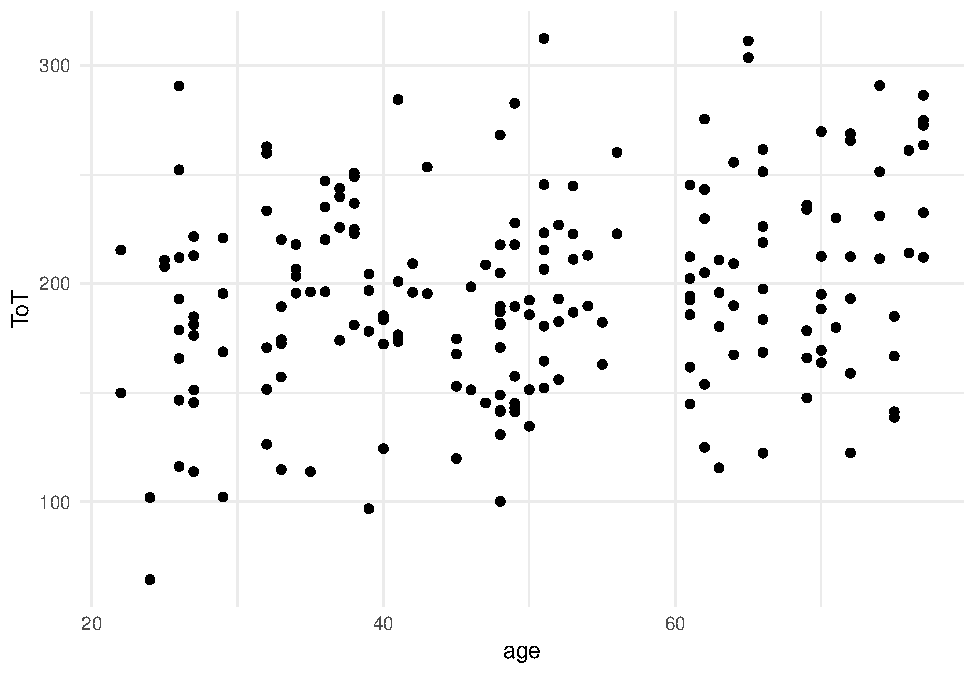
\includegraphics{Getting_started_with_R_files/figure-latex/build_ggpl_2-1.pdf}

Let's take a look at the elements of the command chain: The first two
lines pipe the data frame into the ggplot engine.

\begin{Shaded}
\begin{Highlighting}[]
\NormalTok{BAB1 }\OperatorTok\StringTok{ }
\StringTok{  }\KeywordTok{ggplot}\NormalTok{(...)}
\end{Highlighting}
\end{Shaded}

At that moment, the ggplot engine ``knows'' which variables the data
frame contains and hence are available for the plot. It does not yet
know, which variables are being used, and how. The next step is,
usually, to consider a basic (there exist more than 30) \emph{geometry}
and put it on a \emph{layer}. The scatter plot geometry of ggplot is
\texttt{geom\_point}:

\begin{Shaded}
\begin{Highlighting}[]
\NormalTok{BAB1 }\OperatorTok\StringTok{ }
\StringTok{  }\KeywordTok{ggplot}\NormalTok{(...) }\OperatorTok{+}
\StringTok{  }\KeywordTok{geom_point}\NormalTok{()}
\end{Highlighting}
\end{Shaded}

The last step is the \emph{aesthetic mapping}, which tells ggplot the
variables to use and how to map them to \emph{aesthetic} properties of
the geometry. The basic properties of points in a coordinate system are
the x and y-positions:

\begin{Shaded}
\begin{Highlighting}[]
\NormalTok{BAB1 }\OperatorTok\StringTok{ }
\StringTok{  }\KeywordTok{ggplot}\NormalTok{(}\KeywordTok{aes}\NormalTok{(}\DataTypeTok{x =}\NormalTok{ age, }\DataTypeTok{y =}\NormalTok{ ToT)) }\OperatorTok{+}
\StringTok{  }\KeywordTok{geom_point}\NormalTok{()}
\end{Highlighting}
\end{Shaded}

The function \texttt{aes} creates a mapping where the aesthetics per
variable are given. When call \texttt{aes} directly, we see that it is
just a table.

\begin{Shaded}
\begin{Highlighting}[]
\KeywordTok{aes}\NormalTok{(}\DataTypeTok{x =}\NormalTok{ age, }\DataTypeTok{y =}\NormalTok{ ToT)}
\end{Highlighting}
\end{Shaded}

\begin{verbatim}
## Aesthetic mapping: 
## * `x` -> `age`
## * `y` -> `ToT`
\end{verbatim}

One tiny detail in the above chain has not yet been explained: the
\texttt{+}. When choosing the geometry, you actually \emph{add a layer}
to the plot. This is, of course, not the literal mathematical sum.
Technically, what the author of the ggplot2 package did, was to
\emph{overload} the \texttt{+} operator. A large set of ggplot functions
can be combined in a myriad of ways, just using \texttt{+}. The
overloaded \texttt{+} in ggplot is a brilliant analogy: you can
infinitely chain ggplot functions, like you can create long sums. You
can store ggplot object and later modify it by adding functions. The
analogy has its limits, though: other than sums, order matters in ggplot
combinations: the first in the chain is always \texttt{ggplot} and
layers are drawn upon each other.

Let's move on with a slightly different situation that will result in a
different geometry. Say, we are interested in the distribution of the
time-on-task measures under the two designs. We need a geometry, that
visualizes the distribution of quantitative variables split by a
grouping variable, factor. The box plot does the job:

\begin{Shaded}
\begin{Highlighting}[]
\NormalTok{BAB1 }\OperatorTok\StringTok{ }
\StringTok{  }\KeywordTok{ggplot}\NormalTok{(}\KeywordTok{aes}\NormalTok{(}\DataTypeTok{x =}\NormalTok{ Design,  }\DataTypeTok{y =}\NormalTok{ ToT)) }\OperatorTok{+}
\StringTok{  }\KeywordTok{geom_boxplot}\NormalTok{()}
\end{Highlighting}
\end{Shaded}

\includegraphics{Getting_started_with_R_files/figure-latex/unnamed-chunk-31-1.pdf}

The box plot maps ToT to y (again). The factor Design is represented as
a split on the x-axis. Interestingly, the box plot does not represent
the data as raw as in the scatter plot example. The geometry actually
performs an analysis on ToT, which produces five statistics: min, first
quartile, median, third quartile and max. These statistics define the
vertical positions of bars and end points.

Now, we combine all three variables in one plot: how does the
association between ToT and age differ by design? As we have two
quantitative variables, we stay with the scatter plot for now. As we
intend to separate the groups, we need a property of points to
distinguish them. Points offer several additional aesthetics, such as
color, size and shape. We choose color, and add it to the aesthetic
mapping by \texttt{aes}. Note, that it does not matter whether you use
the British or American way of writing (colour vs.~color).

\begin{Shaded}
\begin{Highlighting}[]
\NormalTok{BAB1 }\OperatorTok\StringTok{ }
\StringTok{  }\KeywordTok{ggplot}\NormalTok{(}\KeywordTok{aes}\NormalTok{(}\DataTypeTok{x =}\NormalTok{ age,  }\DataTypeTok{y =}\NormalTok{ ToT, }\DataTypeTok{color =}\NormalTok{ Design)) }\OperatorTok{+}
\StringTok{  }\KeywordTok{geom_point}\NormalTok{()}
\end{Highlighting}
\end{Shaded}

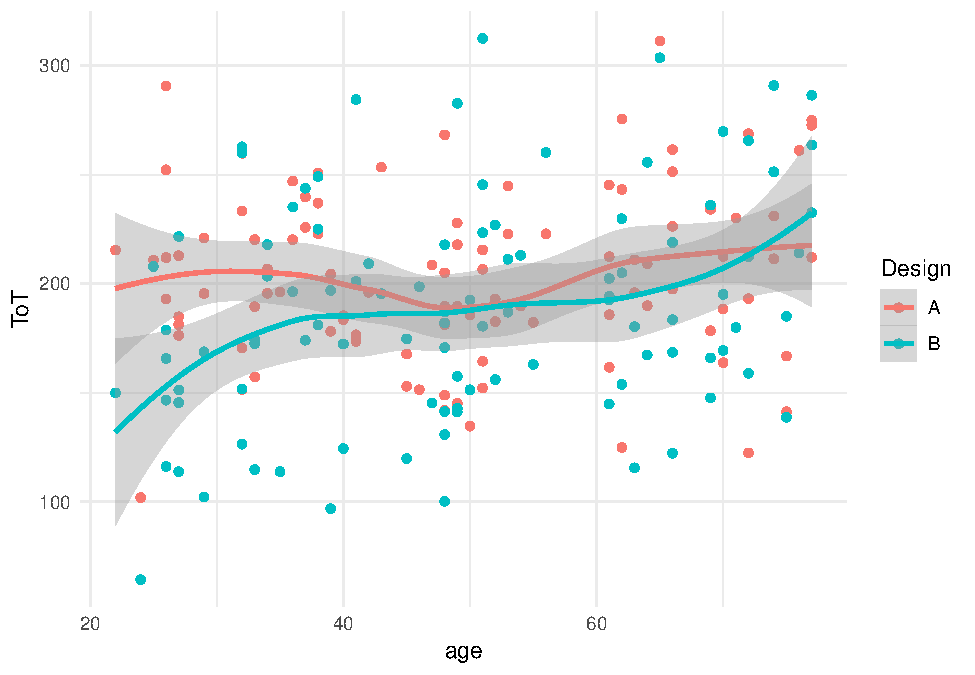
\includegraphics{Getting_started_with_R_files/figure-latex/unnamed-chunk-32-1.pdf}

Now, we can distinguish the groups visually, but there is too much
clutter to discover any relation. With the box plot we saw that some
geometries do not represent the raw data, but summaries (statistics) of
data. For scatter plots, a geometry that does the job of summarizing the
trend is \texttt{geom\_smooth}. This geometry summarizes a cloud of
points by drawing a LOESS-smooth line through it. Note how the color
mapping is applied to all geometry layers.

\begin{Shaded}
\begin{Highlighting}[]
\NormalTok{BAB1 }\OperatorTok\StringTok{ }
\StringTok{  }\KeywordTok{ggplot}\NormalTok{(}\KeywordTok{aes}\NormalTok{(}\DataTypeTok{x =}\NormalTok{ age,  }\DataTypeTok{y =}\NormalTok{ ToT, }\DataTypeTok{color =}\NormalTok{ Design)) }\OperatorTok{+}
\StringTok{  }\KeywordTok{geom_point}\NormalTok{() }\OperatorTok{+}
\StringTok{  }\KeywordTok{geom_smooth}\NormalTok{()}
\end{Highlighting}
\end{Shaded}

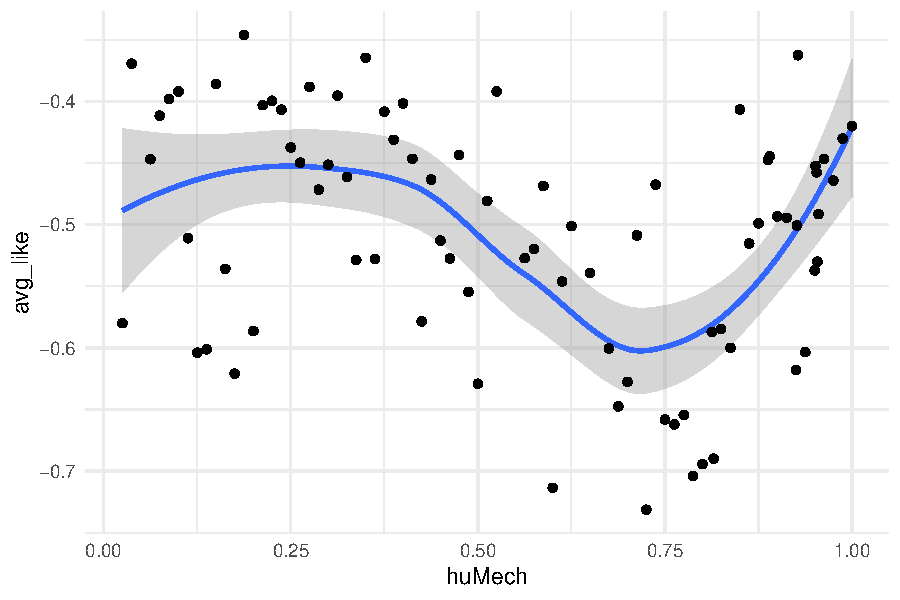
\includegraphics{Getting_started_with_R_files/figure-latex/unnamed-chunk-33-1.pdf}

We see a highly interesting pattern: the association between age and ToT
follows two slightly different mirrored sigmoid curves.

Now that we have represented three variables with properties of
geometries, what if we wanted to add a fourth one, say education level?
Formally, we could use another aesthetic, say shape of points, to
represent it. You can easily imagine that this would no longer result in
a clear visual figure. For situations, where there are many factors, or
factors with many levels, it is impossible to reasonably represent them
in one plot. The alternative is to use \emph{facetting}. A facet splits
the data by a grouping variable and creates one single plot for every
group:

\begin{Shaded}
\begin{Highlighting}[]
\NormalTok{BAB1 }\OperatorTok\StringTok{ }
\StringTok{  }\KeywordTok{ggplot}\NormalTok{(}\KeywordTok{aes}\NormalTok{(}\DataTypeTok{x =}\NormalTok{ age,  }\DataTypeTok{y =}\NormalTok{ ToT, }\DataTypeTok{color =}\NormalTok{ Design)) }\OperatorTok{+}
\StringTok{  }\KeywordTok{geom_point}\NormalTok{() }\OperatorTok{+}
\StringTok{  }\KeywordTok{geom_smooth}\NormalTok{() }\OperatorTok{+}
\StringTok{  }\KeywordTok{facet_grid}\NormalTok{(Education }\OperatorTok{~}\StringTok{ }\NormalTok{.)}
\end{Highlighting}
\end{Shaded}

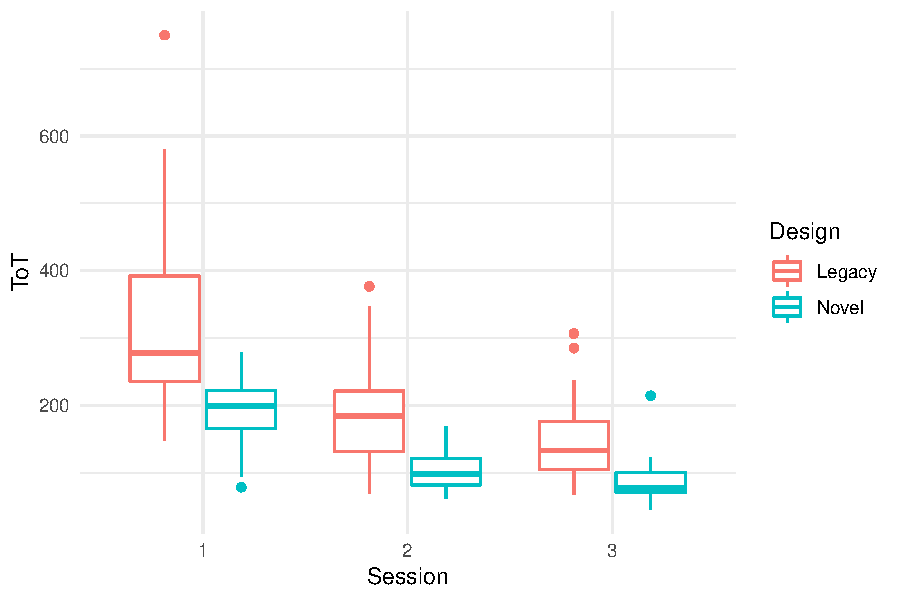
\includegraphics{Getting_started_with_R_files/figure-latex/unnamed-chunk-34-1.pdf}

See, how the \texttt{facet\_grid} command takes a formula, instead of
just a variable name. This makes faceting the primary choice for
highly-dimensional situations. For example, we may also choose to
represent both factors, Design and education by facets:

\begin{Shaded}
\begin{Highlighting}[]
\NormalTok{BAB1 }\OperatorTok\StringTok{ }
\StringTok{  }\KeywordTok{ggplot}\NormalTok{(}\KeywordTok{aes}\NormalTok{(}\DataTypeTok{x =}\NormalTok{ age,  }\DataTypeTok{y =}\NormalTok{ ToT)) }\OperatorTok{+}
\StringTok{  }\KeywordTok{geom_point}\NormalTok{() }\OperatorTok{+}
\StringTok{  }\KeywordTok{geom_smooth}\NormalTok{() }\OperatorTok{+}
\StringTok{  }\KeywordTok{facet_grid}\NormalTok{(Education }\OperatorTok{~}\StringTok{ }\NormalTok{Design)}
\end{Highlighting}
\end{Shaded}

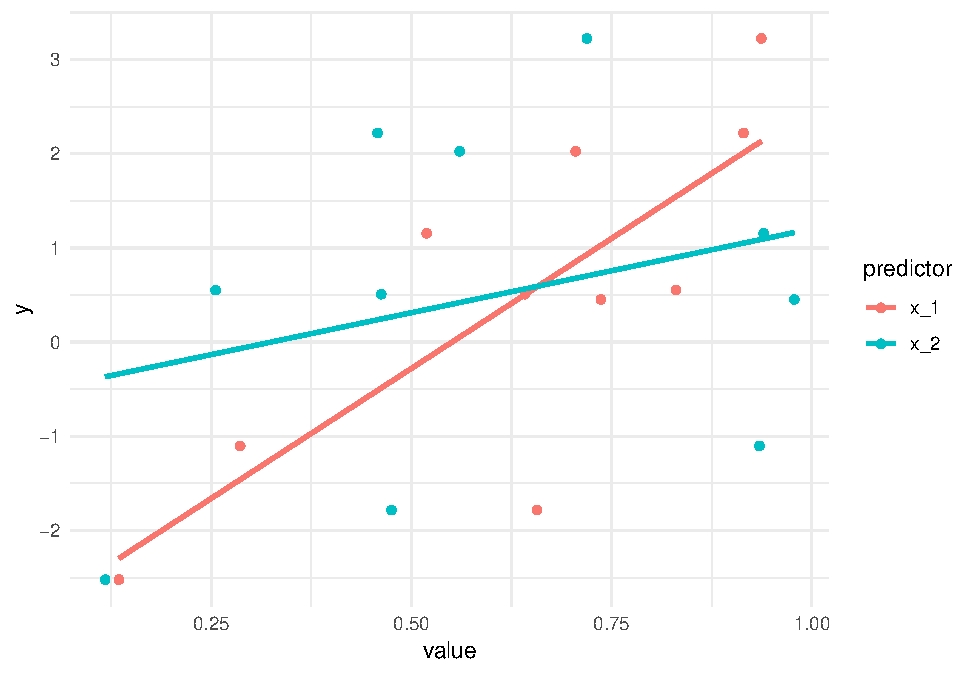
\includegraphics{Getting_started_with_R_files/figure-latex/unnamed-chunk-35-1.pdf}

Note how the color aesthetic, although unnecessary, is kept. It is
possible to map several aesthetics (or facets) to one variable, but not
vice versa.

\subsection{Fitting regression models}\label{fitting-regression-models}

Above we have seen examples of functions that boil down a vector to a
single statistic, like the mean. R has several functions that summarize
data in a more complex way. One function with a wide range of
applications is the \texttt{lm} command, that applies regression models
to data (provided as data frames).

In the following, we will use another simulated data frame \texttt{Exp}
to demonstrate linear models. To make this more interesting, we simulate
\texttt{Exp} in a slightly advanced way, with quantitative associations
between variables. Note how the \emph{expected value} \(\mu\) is created
by drawing on the variables \texttt{Condition} and \texttt{age}. The
last step adds (somewhat) realistic noise to the measures, by drawing
from the normal distribution with a mean of \(mu\).

\begin{Shaded}
\begin{Highlighting}[]
\NormalTok{N_Obs <-}\StringTok{ }\DecValTok{20}
\KeywordTok{set.seed}\NormalTok{(}\DecValTok{42}\NormalTok{)}
\NormalTok{Exp <-}
\StringTok{  }\KeywordTok{data_frame}\NormalTok{(}\DataTypeTok{Obs =} \DecValTok{1}\OperatorTok{:}\NormalTok{N_Obs,}
             \DataTypeTok{Condition =} \KeywordTok{rep}\NormalTok{(}\KeywordTok{c}\NormalTok{(}\StringTok{"Experimental"}\NormalTok{, }\StringTok{"Control"}\NormalTok{),}
\NormalTok{                             N_Obs}\OperatorTok{/}\DecValTok{2}\NormalTok{),}
             \DataTypeTok{age =} \KeywordTok{runif}\NormalTok{(N_Obs, }\DecValTok{18}\NormalTok{, }\DecValTok{35}\NormalTok{),}
             \DataTypeTok{mu =} \DecValTok{200} \OperatorTok{+}\StringTok{ }\NormalTok{(Condition }\OperatorTok{==}\StringTok{ "Control"}\NormalTok{) }\OperatorTok{*}\StringTok{ }\DecValTok{50} \OperatorTok{+}\StringTok{ }\NormalTok{age }\OperatorTok{*}\StringTok{ }\DecValTok{1}\NormalTok{,}
             \DataTypeTok{outcome =} \KeywordTok{rnorm}\NormalTok{(N_Obs, mu, }\DecValTok{10}\NormalTok{))}
\end{Highlighting}
\end{Shaded}

The experiment involves two groups, which in classic statistics would
clearly point to what is commonly referred to as \emph{ANOVA}. As it
will turn out in {[}LM{]}, old-fashioned ANOVA can be replaced by a
rather simple regression model, that I call comparison of groups model
(CGM). The estimation of regression models is done by a \emph{regression
engine}, which basically is a (very powerful) R command. The
specification for any regression model is given in R's formula language.
Learning this formula language is key to unleashing the power of
regression models in R. We can perform a CGM on the data frame
\texttt{Exp} using the regression engine \texttt{stan\_glm}. The desired
model estimates the effect of \texttt{Condition} on \texttt{outcome}.
This produces a regression object that contains an abundance of
information, much of it is of little interest for now. (A piece of
information, that it does \emph{not} contain is F-statistics and
p-values; and that is why it is not an ANOVA, strictly speaking!) The
foremost question is how strong the difference between the groups is.
The \texttt{fixef} command extracts the parameter estimates from the
model to answer the question.

\begin{Shaded}
\begin{Highlighting}[]
\NormalTok{M_}\DecValTok{1}\NormalTok{ <-}\StringTok{ }
\StringTok{  }\KeywordTok{stan_glm}\NormalTok{(outcome }\OperatorTok{~}\StringTok{ }\NormalTok{Condition, }
     \DataTypeTok{data =}\NormalTok{ Exp)}
\end{Highlighting}
\end{Shaded}

\begin{Shaded}
\begin{Highlighting}[]
\KeywordTok{fixef}\NormalTok{(M_}\DecValTok{1}\NormalTok{)}
\end{Highlighting}
\end{Shaded}

\begin{longtable}[]{@{}lrrr@{}}
\toprule
fixef & center & lower & upper\tabularnewline
\midrule
\endhead
Intercept & 274.0 & 266 & 282.4\tabularnewline
ConditionExperimental & -46.1 & -58 & -34.5\tabularnewline
\bottomrule
\end{longtable}

Another classic model is \emph{linear regression}, where outcome is
predicted by a metric variable, say \texttt{age}. The \texttt{stan\_glm}
regression engine is truly multi-purpose and does the job with grace:

\begin{Shaded}
\begin{Highlighting}[]
\NormalTok{M_}\DecValTok{2}\NormalTok{ <-}\StringTok{ }
\StringTok{  }\KeywordTok{stan_glm}\NormalTok{(outcome }\OperatorTok{~}\StringTok{ }\NormalTok{age, }
     \DataTypeTok{data =}\NormalTok{ Exp)}
\end{Highlighting}
\end{Shaded}

\begin{Shaded}
\begin{Highlighting}[]
\KeywordTok{fixef}\NormalTok{(M_}\DecValTok{2}\NormalTok{)}
\end{Highlighting}
\end{Shaded}

\begin{longtable}[]{@{}lrrr@{}}
\toprule
fixef & center & lower & upper\tabularnewline
\midrule
\endhead
Intercept & 206.60 & 126.1 & 285.79\tabularnewline
age & 1.58 & -1.2 & 4.46\tabularnewline
\bottomrule
\end{longtable}

If you are interested in both at the same time, you can combine that in
one model by the following formula:

\begin{Shaded}
\begin{Highlighting}[]
\NormalTok{M_}\DecValTok{3}\NormalTok{ <-}\StringTok{ }
\StringTok{  }\KeywordTok{stan_glm}\NormalTok{(outcome }\OperatorTok{~}\StringTok{ }\NormalTok{Condition }\OperatorTok{+}\StringTok{ }\NormalTok{age, }
     \DataTypeTok{data =}\NormalTok{ Exp)}
\end{Highlighting}
\end{Shaded}

\begin{Shaded}
\begin{Highlighting}[]
\KeywordTok{fixef}\NormalTok{(M_}\DecValTok{3}\NormalTok{)}
\end{Highlighting}
\end{Shaded}

\begin{longtable}[]{@{}lrrr@{}}
\toprule
fixef & center & lower & upper\tabularnewline
\midrule
\endhead
Intercept & 231.69 & 199.310 & 265.46\tabularnewline
ConditionExperimental & -46.21 & -56.362 & -36.43\tabularnewline
age & 1.51 & 0.344 & 2.66\tabularnewline
\bottomrule
\end{longtable}

A statistical model has several components, for example the coefficients
and residuals. Models are complex objects, from which a variety of
inferences can be made. For example, the coefficient estimates can be
extracted and used for prediction. This is what \texttt{fixef()} does in
the above code.

A number of functions can be used to extract certain aspects of the
model. For example:

\begin{itemize}
\tightlist
\item
  \texttt{fixef(model)} extracts the linear effects
\item
  \texttt{residuals(model)} extracts the measurement errors
\item
  \texttt{predict(model)} extracts the expected values
\end{itemize}

These will all be covered in later chapters.

\subsection{Knitting statistical
reports}\label{knitting-statistical-reports}

As you have seen throughout this chapter, with R you can effectively
manage data, create impressively expressive graphics and conveniently
estimate statistical models. Then usually comes the painful moment where
all this needs to be assembled into a neat report. With R and Rstudio it
has never been easier than that. In fact, complete books have been
written in R, like the one you are reading.

A \emph{minimal statistical report} contains four elements:

\begin{enumerate}
\def\labelenumi{\arabic{enumi}.}
\tightlist
\item
  a recap of the research question
\item
  description of how the statistical model relates to the research
  question
\item
  a few figures or tables that answers the research question
\item
  an explanation of the results
\end{enumerate}

Of these four elements, three are pure text. For a minimal report it is
a fairly convenient to use a word processor software for the text, craft
the figure in R and copy it. One problem with this approach is that a
\emph{scrunitable statistical report} contains at least the following
\emph{additional} elements:

\begin{enumerate}
\def\labelenumi{\arabic{enumi}.}
\tightlist
\item
  procedures of data preparation (sources, transformations, variable
  names, outlier removal)
\item
  data exploration (ranges of variables, outlier discovery, visualizing
  associations, etc.)
\item
  model estimation (formula specification, convergence checks)
\item
  model criticism (normality of residuals, etc.)
\end{enumerate}

In advanced statistical workflows this is then multiplied by the number
of models, an iterative selection process. Because it is easy to lie
with statistics, these elements are needed as to build a fundament of
credibility. Full transparency is achieved, when another researcher can
exactly reproduce all steps of the original analysis. It is obvious that
the easiest way to achieve this, is to hand over the full R script.

The most user-friendly way to achieve both, a good looking report and
full transparency, is to write a document that contains all before
mentioned: text, graphics, tables and R code. In the R environment such
mixed documents can be written in the \emph{markdown/knitr} framework.

Markdown implements a simple markup language, with that you can typset
simple, structured texts in a plain ASCII editor. Later in the workflow,
such a markup document is transformed into one of various output
formats, that are rendered by the respective programs, such as Microsoft
Word or an HTML browser.

\begin{figure}
\centering
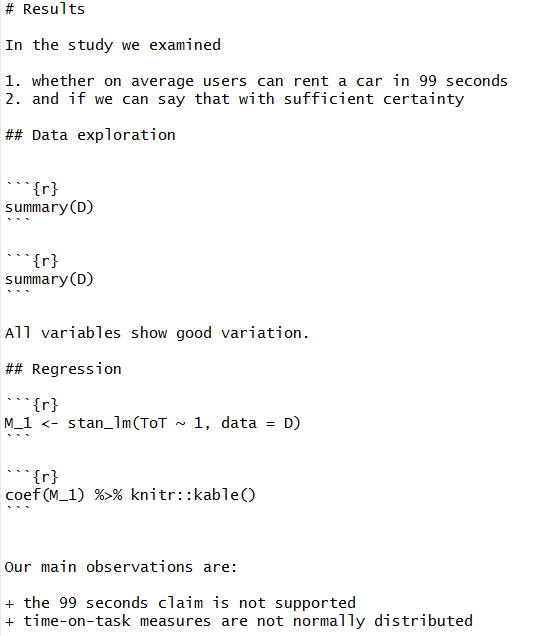
\includegraphics{Illustrations/markup_minimal_report.png}
\caption{A minimal statistical report in markdown}
\end{figure}

The above text is an alternation of markup text and \emph{chunks}, those
weirdly enclosed pieces of R code. While the text is static, the chunks
are processed by the knitr engine, evaluating the enclosed R code and
knitting the output into a document. Very conveniently, when the output
is a figure, it will be inserted into the document right away. The
\texttt{kable} command from the knitr package, in turn, produces neatly
rendered tables from data frame objects. By default, the R code is
shown, too, but that can be customized.

The minimal workflow for statistical reporting with knitr is as follows:

\begin{enumerate}
\def\labelenumi{\arabic{enumi}.}
\tightlist
\item
  Use markdown right away, covering all steps of your data analysis,
  i.e.~a scrutable report. You may even start writing when only one part
  of your data gathering is completed, because due to the dynamic
  chunks, updating the report when new data arrives is just a button
  click away.
\item
  When the data analysis is complete, compile the scrutable report to
  Word format
\item
  Extract the passages, figures and tables for a minimal statistical
  report. This is your results section.
\item
  provide the scrutable report as appendix or supplementary material
\end{enumerate}

In the notion of this chapter, this is just to get you started and knitr
is so tightly integrated with the Rstudio environment that I don't even
bother to explain the commands for knitting a document. Once acquainted
with the basics, markdown provides a few additional markup tokens, like
footnotes, hyperlinks or including images. The customization options and
addons for knitr are almost endless and various interesting addons are
available, just to mention two:

\begin{enumerate}
\def\labelenumi{\arabic{enumi}.}
\tightlist
\item
  The bookdown package provides an infrastructure for writing and
  publishing longer reports and books.
\item
  With the shiny package one can add dynamic widgets to HTML reports.
  Think of a case, where your statistical model is more complicated than
  a linear regression line or a few group means, say you are estimating
  a polynomial model or a learning curve. Then, with a simple shiny app,
  you can enable your readers to understand the model by playful
  exploration.
\end{enumerate}

\subsection{Exercises}\label{exercises-1}

\begin{enumerate}
\def\labelenumi{\arabic{enumi}.}
\item
  In the book package (directory \texttt{/Data}) you will find the data
  set of the (virtual) study BAB1, which we will be using in coming
  chapters. This data comes as comma-separated value file with the file
  ending \texttt{.csv}. Load this file into R using the
  \texttt{read\_csv} command and check the dataframe.
\item
  Find the documentation of the packages \texttt{haven} and
  \texttt{readr}. Find two import functions. The one that is most useful
  for you and the one that you consider most exotic.
\item
  We have seen how to extract a data frame column as a vector using the
  double square brackets. There seems to be no such option to extract an
  individual row as a vector. Why? (Think about object types).
  \textless{}--! \#14 --\textgreater{}
\item
  Use the world wide web to find geometries that are useful for plotting
  associations between grouping variables (factors) and a metric
  variables. Try them all on the BAB1 data frame. Compare the geometries
  on what properties of the data they convey.
\item
  Like data frames and regression results, plots produced by ggplot are
  complex objects, too. Create an arbitrary plot, store it in a variable
  and inspect it using \texttt{class}, \texttt{summary} and
  \texttt{str}. In addition, what happens when you assign the plot to a
  variable and what happens when you call the variable?
\item
  Revisit the python-swallowed-camel plot and check out how the
  aesthetic mapping is created. The plot uses a density geometry. Change
  it into a histogram. Then produce a box plot that shows the two
  conditions (think carefully about the mappings of x and y).
\item
  Use the data set BAB5 in BrowsingAB. It contains a follow-up
  experiment, where participants had to do five different tasks on the
  website. Plot the association between age and ToT by task, using
  color. Then put Task on a facet grid, and use color to represent
  Design again.
\item
  Use the data set BAB5 in BrowsingAB. Using a transformation chain,
  take the sum or average of participants' ToT. Then run a few simple
  regression models.
\item
  Use your own data. Drop an Excel and/or an SPSS file into the same
  directory as your current R file. Read the data into a data frame and
  summarize what is in the data frame. Use ggplot to create one or more
  exploratory graphs. Then use dplyr \texttt{summarize} to create
  summary statistics.
\item
  Do a full exploratory analysis of the dataframe D\_agg in case
  environment IPump. It has the predictors Design, Group, Education and
  experience. It has the outcome variables ToT, deviations and workload.

  \begin{enumerate}
  \def\labelenumii{\arabic{enumii}.}
  \tightlist
  \item
    Get the data frame into R and produce a summary.
  \item
    Plot a histogram for all dependent variables.
  \item
    Produce a table that counts the number of observations per
    Education(al level).
  \item
    Produce a table that displays minimum, maximum, median, mean and
    standard deviation of experience.
  \item
    Exclude participants with less than four years of experience.
  \item
    Produce a table with group means per Design and Session.
  \item
    For every outcome variable, produce a plot for Design by session.
  \item
    Explore graphically, what other relations may exist between outcome
    variables and Group, Education and experience.
  \item
    Run a regression model for ToT with Design and Session as
    predictors.
  \item
    Produce a coefficient table.
  \item
    Plot the residuals.
  \end{enumerate}
\end{enumerate}

\subsection{Bibliographic notes}\label{bibliographic-notes-1}

\href{http://r4ds.had.co.nz/}{R for Data Science} is a book co-authored
by Hadley ``Tidy'' Wickham.

\href{http://www.r-bloggers.com/ggplot2-version-of-figures-in-\%E2\%80\%9C25-recipes-for-getting-started-with-r\%E2\%80\%9D/}{ggplot2
Version of Figures in ``25 Recipes for Getting Started with R''} for
readers who are familiar with the legacy plotting commands in R.

\href{http://rpubs.com/justmarkham/dplyr-tutorial}{Introduction to dplyr
for Faster Data Manipulation in R} introduces dplyr, the next generation
R interface for data manipulation, which is used extensively in this
book.

\href{http://www.statmethods.net/}{Quick-R} is a comprehensive
introduction to many common statistical techniques with R.

\href{http://codeasmanuscript.org/lessons/}{Code as manuscript} features
a small set of lessons with code examples, assignments and further
resources. For if you are in a haste.

\href{https://bookdown.org/yihui/bookdown/}{bookdown: Authoring Books
and Technical Documents with R Markdown} fully unleashes the power of
knitr for writing and publishing longer reports and books.

\part{Models}\label{part-models}

\chapter{Linear models}\label{linear_models}

\section{Quantification at work: grand mean
models}\label{quantification-at-work-grand-mean-models}

Reconsider Andrew and Jane. They were faced with the problem that
potential competitors could challenge the claim ``rent a car in 99
seconds'' and drag them to court. More precisely, the question was:
``will users on average be able \ldots{}'', which is not about
individual users, but the \emph{population mean}. A statistical model
estimating just that we call a \emph{grand mean model} (GMM). The GMM is
the most simple of all models, so in a way, we can think of it as the
``grandmother of all models''. Although its is the simplest of all, it
is of useful application in design research; here are a few more
examples:

\begin{itemize}
\tightlist
\item
  with medical infusion pump the frequency of decimal input error
  (giving the tenfold or the tenth of the prescribed dose) must be below
  a bearable level
\item
  the checkout process of an e-commerce website must have a a cancel
  rate not higher than \ldots{}
\item
  the brake lights of a car must be designed to let the following driver
  react in a certain time frame
\end{itemize}

The GMM predicts the expected level of performance when the only thing
you know is the population someone is from. Prediction here means that
the estimated grand mean we take as a best guess for the population
average, that is all realizations we have \emph{not} observed. So, it is
a generalization regarding all people we have not invited to the lab,
but also potential performance differences by situation, for example the
daily shape people are in or their current level of motivation. Just
consider the many ways people differ in abilities, experience,
strategies, preferences, situations, wishes etc. All these differences
may also vary for the same person from day to day and influence
performance. All these aspects have not been recorded in the Sec99 study
and are therefore not taken into account for prediction. All linear
models capture the unpredicted variation in a separate parameter
\(\sigma\), the \emph{residual standard deviation}. \(\sigma\) measures
the amount of variance that is left after subtracting all explanatory
variables. Formally, the likelihood and random formulas of the grand
mean model are written with the following likelihood and random term:

\[
\mu = \beta_0\\
y_i \sim \textrm{Norm}(\mu_i, \sigma_\epsilon)
\]

The larger \(\sigma\) is, the more questionnable it is that the grand
mean is truly \emph{representative} for the population. From the GM we
will depart in to directions. First, in the remainder of this chapter,
we will add further predictors to the model, for example age of
participants or a design condition. These models will still make
statements on population averages, although in a more detailed way. In
the following chapter on mixed-effects models, individuals will get spot
light. Still, what all the advanced models have in common is that they
move variance in the outcome variable from the error variance to
predictors. An optimist would say: today's error is tomorrow's
predictor.

So, when estimating the grand mean model, we estimate the intercept
\(\beta_0\) and the standard deviation of the Gaussian distributed error
term \(\sigma\epsilon\). In R, the analysis of the 99 seconds problem
unfolds as follows: completion times (ToT) are stored in a data frame,
with one observation per row. This data frame is send to the R command
\texttt{stan\_glm} for estimation, using \texttt{data\ =\ Ver20}. As the
\texttt{stan\_glm} command applies to a huge variety of regression
model, the desired model needs further specification. For that purpose,
R has its own formula language. The formula of the grand mean model is
\texttt{ToT\ \textasciitilde{}\ 1}. Left of the
\texttt{\textasciitilde{}} (\emph{tilde}) operator is the outcome
variable. The right hand side specifies the deterministic part. The 1
here has nothing to do with the natural number neighboured by 0 and 2.
In R's formula language it represents the \emph{intercept}.

\begin{Shaded}
\begin{Highlighting}[]
\KeywordTok{attach}\NormalTok{(Sec99)}
\end{Highlighting}
\end{Shaded}

\begin{Shaded}
\begin{Highlighting}[]
\NormalTok{M_}\DecValTok{1}\NormalTok{ <-}\StringTok{ }\KeywordTok{stan_glm}\NormalTok{(ToT }\OperatorTok{~}\StringTok{ }\DecValTok{1}\NormalTok{, }\DataTypeTok{data =}\NormalTok{ Ver20)}
\end{Highlighting}
\end{Shaded}

\begin{Shaded}
\begin{Highlighting}[]
\KeywordTok{summary}\NormalTok{(M_}\DecValTok{1}\NormalTok{)}
\end{Highlighting}
\end{Shaded}

\begin{verbatim}
## 
## Model Info:
## 
##  function:     stan_glm
##  family:       gaussian [identity]
##  formula:      ToT ~ 1
##  algorithm:    sampling
##  priors:       see help('prior_summary')
##  sample:       4000 (posterior sample size)
##  observations: 100
##  predictors:   1
## 
## Estimates:
##                 mean   sd     2.5%   25%    50%    75%    97.5%
## (Intercept)    106.0    3.1   99.9  103.8  106.0  108.1  112.0 
## sigma           31.5    2.3   27.5   29.9   31.3   33.0   36.5 
## mean_PPD       106.0    4.5   97.2  103.0  106.0  109.0  114.9 
## log-posterior -494.3    1.0 -497.1 -494.7 -494.0 -493.6 -493.3 
## 
## Diagnostics:
##               mcse Rhat n_eff
## (Intercept)   0.1  1.0  2711 
## sigma         0.0  1.0  2709 
## mean_PPD      0.1  1.0  3258 
## log-posterior 0.0  1.0  1382 
## 
## For each parameter, mcse is Monte Carlo standard error, n_eff is a crude measure of effective sample size, and Rhat is the potential scale reduction factor on split chains (at convergence Rhat=1).
\end{verbatim}

The object \texttt{M\_1} is the model object created by
\texttt{stan\_glm}. When you call the summary you complex listings that
represent different aspects of the regression. These aspects, and more
are saved inside the object in a hierarchy of lists. The central result
of the estimation is the \emph{posterior distribution (PD)}. It is an
array of variables over MCMC runs. We extract the posterior distribution
from the model object using the \texttt{posterior} command (package:
\texttt{bayr}).

\begin{Shaded}
\begin{Highlighting}[]
\NormalTok{P_}\DecValTok{1}\NormalTok{ <-}\StringTok{ }\KeywordTok{posterior}\NormalTok{(M_}\DecValTok{1}\NormalTok{)}
\NormalTok{P_}\DecValTok{1}
\end{Highlighting}
\end{Shaded}

** tbl\_post: 4000 samples in 1 chains

\begin{longtable}[]{@{}lrllr@{}}
\toprule
model & parameter & type & fixef & entities\tabularnewline
\midrule
\endhead
M\_1 & 1 & fixef & Intercept & 1\tabularnewline
\bottomrule
\end{longtable}

\begin{longtable}[]{@{}l@{}}
\toprule
parameter\tabularnewline
\midrule
\endhead
sigma\_resid\tabularnewline
\bottomrule
\end{longtable}

The posterior object identifies itself by telling the number of MCMC
samples, and the variables contained in the model. In the case here,
there is just the intercept (representing the grand mean) and the
standard deviation of errors.

Much of the time a researcher doesn't want to deal with the posterior,
directly, but desires a brief summary of location and uncertainty.
Coefficient tables are frequently used, just like one one shown
below.Coefficient tables report the central tendency of every
coefficient, which is an indicator for the magnitude of an effect. Next
to that, the spread of the posterior distribution is summarized as 95\%
credibility intervals and represent the degree of uncertainty: the less
certain an estimate is, the wider is the interval. A 95\% credibility
interval gives a range of possible values where you can be 95\% certain
that it contains the true value. A coefficient table is produced by the
\texttt{coef} command of the bayr library:

\begin{Shaded}
\begin{Highlighting}[]
\KeywordTok{coef}\NormalTok{(P_}\DecValTok{1}\NormalTok{)}
\end{Highlighting}
\end{Shaded}

\begin{longtable}[]{@{}lllrrr@{}}
\toprule
parameter & type & fixef & center & lower & upper\tabularnewline
\midrule
\endhead
Intercept & fixef & Intercept & 106.0 & 99.9 & 112.0\tabularnewline
sigma\_resid & disp & NA & 31.3 & 27.5 & 36.5\tabularnewline
\bottomrule
\end{longtable}

\begin{Shaded}
\begin{Highlighting}[]
\KeywordTok{detach}\NormalTok{(Sec99)}
\end{Highlighting}
\end{Shaded}

\subsection{Reading coefficient
tables}\label{reading-coefficient-tables}

Coefficient tables are the standard way to report regression models.
They contain all parameters (or a selection of interest) in rows. For
every parameter, the central tendency (center, magnitude, location) is
given, and a statement of uncertainty, by convention 95\% credibility
intervals (CI).

The authors of Bayesian books and the various Bayesian libraries have
different opinions on what to report in a coefficient table. Most seem
to prefer the posterior mode or the median, only some use the mean.

A disadvantage of the \emph{mean} is that it may change, under many
monotonic transformations. A monotonic transformations is a recoding of
a variable \(x_1\) into a new variable \(x_2\) by a transformation
function \(\phi\) (\(phi\)) such that the order of values stays
untouched. Examples of monotonic functions are the logarithm
(\(x_2 = \log(x_1)\)), the exponential function (\(x_2 = \exp(x_1)\)),
or simply \(x_2 = x_1 + 1\). A counter example is the quadratic function
\(x_2 = x_1^2\). In data analysis monotonous transformations are used a
lot. Especially, Generalized Linear Models make use of monotonous link
functions to establish linearity \ref{re-linking-linearity}.

The \emph{mode} of a distribution is its point of highest density. It is
invariant under monotonic transformations. It also has a rather
intuitive meaning as the most likely value for the true parameter. Next
to that, the mode is compatible with classic maximum likelihood
estimation. When a Bayesian takes a pass on any prior information, the
posterior mode should precisely match the results of a classic
regression engine (e.g., \texttt{glm}). The main disadvantage of the
mode is that it has to be estimated by one of several heuristic
algorithms. These add some computing time and may fail when the
posterior distribution is bi-modal. However, when that happens, you
probably have a more deeply rooted problem, than just deciding on a
suitable summary statistic.

The \emph{median} of a distribution marks the point where half the
values are below and the other half are equal or above. Technically, the
median is just the 50\% quartile of the distribution. The median is
extremely easy and reliable to compute, and it shares the invariance of
monotonous transformations. This is easy to conceive: The median is
computed by ordering all values in a row and then picking the value that
is exactly in the middle. Obviously, this values only changes when the
order changes, i.e.~a non-monotonous function was applied.

For center estimates I use the posterior median by default, for its
simplicity. Researchers who desire downward compatibility with classic
regression engines, can easily switch to the mode by using the
\(estimate\) argument. The following uses the \texttt{shorth} command
form the package \texttt{modeest}.

\begin{Shaded}
\begin{Highlighting}[]
\KeywordTok{attach}\NormalTok{(Sec99)}
\end{Highlighting}
\end{Shaded}

\begin{Shaded}
\begin{Highlighting}[]
\KeywordTok{coef}\NormalTok{(P_}\DecValTok{1}\NormalTok{, }\DataTypeTok{estimate =}\NormalTok{ modeest}\OperatorTok{::}\NormalTok{shorth)}
\end{Highlighting}
\end{Shaded}

\begin{longtable}[]{@{}lllrrr@{}}
\toprule
parameter & type & fixef & center & lower & upper\tabularnewline
\midrule
\endhead
Intercept & fixef & Intercept & 106.0 & 99.9 & 112.0\tabularnewline
sigma\_resid & disp & NA & 31.1 & 27.5 & 36.5\tabularnewline
\bottomrule
\end{longtable}

Expressing the level of certainty of the posterior distribution makes
statistics \emph{inferential}. When the posterior is widely spread, you
will still bet on values close to the center, but keep your bid low. For
the spread of a distribution, the standard deviation may come to mind of
some readers. The standard deviation has teh disadvantage that a single
value does not represent non-symmetric distributions well. A better way
is to express certainty as limits, a lower and an upper. The most simple
method resembles that of the median by using quantiles. In this book,
\emph{2.5\% and 97.5\% certainty quantiles} are routinely used to form
95\% credibility intervals. Again, another method exists to obtain CIs.
Some authors prefer to report the \emph{highest posterior interval},
which is the narrowest interval that contains 95\% of the probability
mass. While this is intriguing to some extent, HPDs are not invariant to
monotonic transformations.

The \texttt{coef} command by default gives the median and the 2.5\% and
97.5\% limits. The three parameters have in common that they are
quantiles, which are handled by Rs \texttt{quantile} command. To
demystify the \texttt{coef}, here is how you can make a basic
coefficient table yourself:

\begin{Shaded}
\begin{Highlighting}[]
\NormalTok{P_}\DecValTok{1} \OperatorTok
\StringTok{  }\KeywordTok{group_by}\NormalTok{(parameter) }\OperatorTok\StringTok{ }
\StringTok{  }\KeywordTok{summarize}\NormalTok{(}\DataTypeTok{center =} \KeywordTok{quantile}\NormalTok{(value, }\FloatTok{0.5}\NormalTok{),}
         \DataTypeTok{lower  =} \KeywordTok{quantile}\NormalTok{(value, }\FloatTok{0.025}\NormalTok{),}
         \DataTypeTok{upper  =} \KeywordTok{quantile}\NormalTok{(value, }\FloatTok{0.975}\NormalTok{)) }\OperatorTok\StringTok{ }
\StringTok{  }\KeywordTok{kable}\NormalTok{()}
\end{Highlighting}
\end{Shaded}

\begin{tabular}{l|r|r|r}
\hline
parameter & center & lower & upper\\
\hline
Intercept & 106.0 & 99.9 & 112.0\\
\hline
sigma\_resid & 31.3 & 27.5 & 36.5\\
\hline
\end{tabular}

Note that we get CIs for the dispersion parameter \(\sigma\), too. Many
classic analyses call \(\sigma\) are nuisance parameter and ignore it,
or they blame high variation between observations for not reaching
``significant'' certainty for the parameter of interest. Furthermore,
classic regression engines don't yield and measures of certainty on
dispersion parameters. I believe that understanding the amount of
variation is often crucial for design research and several of the
examples that follow try to make the case. This is why we should be glad
that Bayesian engines report uncertainty on all parameters involved.

It is common practice to not just drop coefficient tables, but explain
and interpret them in written form. My suggestion of how to \emph{report
regression results} is to simply walk through the table row-by-row and
for every parameter make two statements: a quantitative statement based
on the central tendency, and an uncertainty statement. In the present
case that would be:

\begin{enumerate}
\def\labelenumi{\arabic{enumi}.}
\tightlist
\item
  The \emph{intercept} \(\beta_0\) is in the region of 106 seconds,
  which is pretty off the target of 99 seconds.
\item
  The certainty is pretty good. At least we can say that the chance of
  the true mean being 99 seconds or smaller is pretty marginal, as it is
  not even contained in the 95\% CI.
\end{enumerate}

And for \(\sigma\):

\begin{enumerate}
\def\labelenumi{\arabic{enumi}.}
\tightlist
\item
  The population mean is rather not representative for the observations,
  as the standard error is almost one third of it.
\item
  We can be pretty certain that this is so.
\end{enumerate}

\begin{Shaded}
\begin{Highlighting}[]
\KeywordTok{detach}\NormalTok{(Sec99)}
\end{Highlighting}
\end{Shaded}

\subsection{Likelihood and random
term}\label{likelihood-and-random-term}

In formal language, regression models are usually specified by
\emph{likelihood functions} and one or more \emph{random terms} (exactly
one in linear models). The likelihood represents the common, predictable
pattern in the data. Formally, the likelihood establishes a link between
\emph{predicted values} \(mu_i\) and predictors. It is common to call
predictors with the Greek letter \(\beta\) (beta). If there are more
than one predictors, these are marked with subscripts, starting at zero.
The ``best guess'' is called the \emph{expected value} and is denoted
with \(\mu\) (mu\_i). If you just know that the average ToT is 106
seconds and you are asked to guess the performance of the next user
arriving in the lab, the reasonable guess is just that, 106 seconds.

\[\mu_i = \beta_0\]

Of course, we would never expect this person to use 106 second, exactly.
All observed and imagined observations are more or less clumped around
the expected value. The \emph{random term} specifies our assumptions on
the pattern of randomness. It is given as a distributions (note the
plural), denoted by the \(\sim\) (tilde) operator, which reads as: ``is
distributed''. In the case of linear models, the assumed distribution is
always the Normal or \emph{Gaussian distribution}. Gaussian
distributions have a characteristic bell curve and depend on two
parameters: the mean \(\mu\) as the central measure and the standard
deviation \(\sigma\) giving the spread.

\[y_i \sim N(\mu_i, \sigma_{\epsilon})\]

The random term specifies how all unknown sources of variation take
effect on the measures, and these are manifold. Randomness can arise due
to all kinds of individual differences, situational conditions and, last
but not least, measurement errors. The Gaussian distribution often is a
good approximation for randomness and linear models are routinely used
in research. In several classic statistics books, the following formula
is used to describe the GMM (and likewise more complex linear models):

\[
y_i = \mu_i + \epsilon_i\\
\mu_i = \beta_0\\
\epsilon_i \sim \textrm{Norm}(0, \sigma_\epsilon)
\]

First, it is to say, that the two ways of formula are mathematically
equivalent. The primary difference to our formula is that the
\emph{residuals \(\epsilon_i\)}, are given separately. The pattern of
residuals is then specified as a single Normal distribution. Residual
distributions are a highly useful concept in modelling as they can be
used to check a given model. When residuals are such a highly useful
concept, the classic formula is more intuitive. The reason for
separating the model into likelihood and random term is that it works in
more cases. When turning to Generalized Linear Models (GLM) in chapter
\ref{generalized-linear-models}, we will use other patterns of
randomness, that are no longer additive, like in \(\mu_i + \epsilon_i\).
As I consider the use of GLMs an element of professional statistical
practice, I use the general formula right from the start.

\subsection{Do the random walk: Markov Chain Monte Carlo
sampling}\label{random_walk}

So far, we have seen how linear models are specified and how,parameters
are interpreted from standard coefficient table. While it is convenient
to have a standard procedure it turns out very useful to understand how
these estimates came to life. In Bayesian estimation, the
\emph{posterior distribution (PD)} is the central point of departure for
any such statements. The PD assigns a degree of certainty for every
possible combination of parameter values. In the current case, you can
ask the PD, where and how certain the population mean and the residual
standard error are, but you can also ask: How certain are we that the
population mean is smaller than 99 seconds and \(\sigma\) is smaller
than 10?

In a perfect world, we would know the analytic formula of the posterior
and derive statements from it. In most non-trivial cases, though, there
is no such formula one can work with. Instead, what the regression
engine does is to approximate the PD by a random-walk algorithm called
Markov-Chain Monte Carlo sampling (MCMC).

In fact, the \texttt{stan\_glm} command returns a large object that
stores, among others, the full random walk. This random walk represent
the posterior distribution almost directly. The following code extracts
this the posterior distribution from the regression object prints it.
When calling the new object (class: tbl\_post) directly, it provides a
compact summary of all variables in the model, here this is the
intercept and the residual standard error.

\begin{Shaded}
\begin{Highlighting}[]
\KeywordTok{attach}\NormalTok{(Sec99)}
\end{Highlighting}
\end{Shaded}

\begin{Shaded}
\begin{Highlighting}[]
\NormalTok{P_}\DecValTok{1}\NormalTok{ <-}\StringTok{  }\KeywordTok{posterior}\NormalTok{(M_}\DecValTok{1}\NormalTok{)}
\NormalTok{P_}\DecValTok{1}
\end{Highlighting}
\end{Shaded}

** tbl\_post: 4000 samples in 1 chains

\begin{longtable}[]{@{}lrllr@{}}
\toprule
model & parameter & type & fixef & entities\tabularnewline
\midrule
\endhead
M\_1 & 1 & fixef & Intercept & 1\tabularnewline
\bottomrule
\end{longtable}

\begin{longtable}[]{@{}l@{}}
\toprule
parameter\tabularnewline
\midrule
\endhead
sigma\_resid\tabularnewline
\bottomrule
\end{longtable}

The 99 second GMM has two parameters and therefore the posterior
distribution has three dimensions: the parameter dimensions \(\beta_0\),
\(\sigma\) and the probability density. Three dimensional plots are
difficult to put on a surface, but for somewhat regular patterns, a
density plot with contour lines do a sufficient job:

\begin{Shaded}
\begin{Highlighting}[]
\NormalTok{P_}\DecValTok{1} \OperatorTok\StringTok{ }
\StringTok{  }\KeywordTok{select}\NormalTok{(chain, iter, parameter, value) }\OperatorTok\StringTok{ }
\StringTok{  }\KeywordTok{spread}\NormalTok{(parameter, value) }\OperatorTok\StringTok{ }
\StringTok{  }\KeywordTok{ggplot}\NormalTok{(}\KeywordTok{aes}\NormalTok{(}\DataTypeTok{x =}\NormalTok{ Intercept, }\DataTypeTok{y =}\NormalTok{ sigma_resid, }\DataTypeTok{fill =}\NormalTok{ ..level..)) }\OperatorTok{+}
\StringTok{  }\KeywordTok{stat_density_2d}\NormalTok{(}\DataTypeTok{geom =} \StringTok{"polygon"}\NormalTok{) }\OperatorTok{+}
\StringTok{  }\KeywordTok{xlim}\NormalTok{(}\DecValTok{95}\NormalTok{, }\DecValTok{115}\NormalTok{) }\OperatorTok{+}\StringTok{ }\KeywordTok{ylim}\NormalTok{(}\DecValTok{25}\NormalTok{, }\DecValTok{40}\NormalTok{)}
\end{Highlighting}
\end{Shaded}

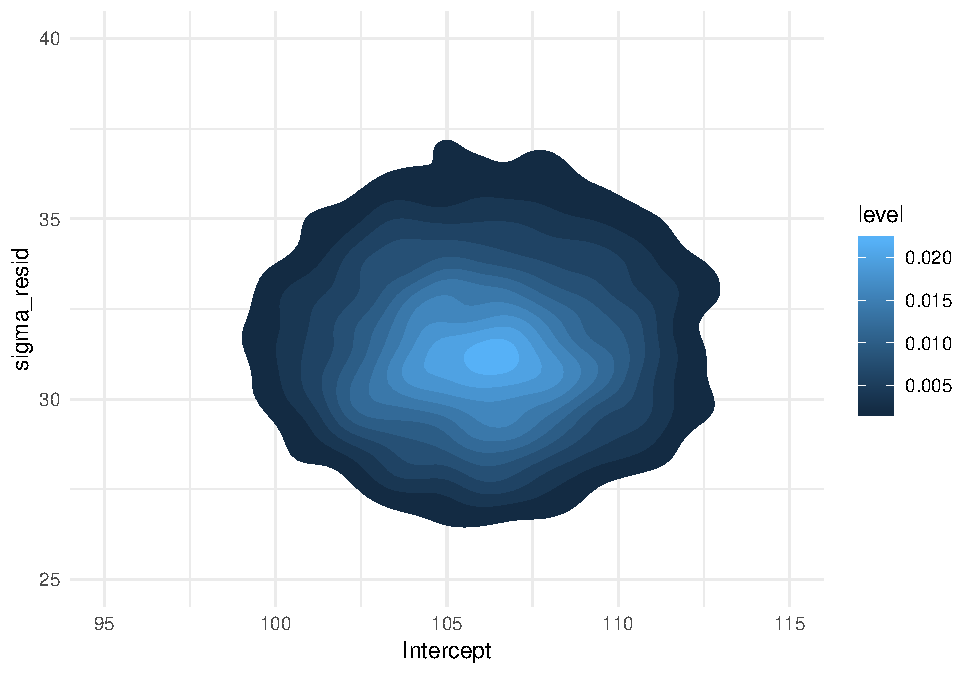
\includegraphics{Classic_linear_models_files/figure-latex/unnamed-chunk-10-1.pdf}

Let's see how this PD ``landscape'' actually emerged from the random
walk. In the current case, the \emph{parameter space} is
two-dimensional, as we have \(\mu\) and \(\sigma\). The MCMC procedure
starts at a deliberate point in parameter space. At every iteration, the
MCMC algorithm attempts a probabilistic jump to another location in
parameter space and stores the coordinates. This jump is called
probabilistic, because it is either carried out, or not, and that
depends on a bet. If the new target is in a highly likely region, it is
carried out with a higher chance. This sounds circular, but it works
and, of course, it has been proven mathematically that it works.

The regression object stores the MCMC results as a long series of
positions in parameter space. For any range of interest, it is the
relative frequency of visits that represents its certainty. The first 50
hundred steps of the MCMC random walk are shown in
@ref(99\_seconds\_random\_walk)`. Apparently, the random walk is not
fully random, as the point cloud is more dense in the center area. This
is where the more probable parameter values lie. One can clearly see how
the MCMC algorithm jumps to more likely areas more frequently. These
areas become more dense and, finally, the cloud of visits will approach
the contour density plot above.

\begin{Shaded}
\begin{Highlighting}[]
\NormalTok{G_random_walk <-}
\StringTok{  }\NormalTok{P_}\DecValTok{1} \OperatorTok\StringTok{ }
\StringTok{  }\KeywordTok{filter}\NormalTok{(iter }\OperatorTok{<=}\StringTok{ }\DecValTok{50}\NormalTok{) }\OperatorTok\StringTok{ }
\StringTok{  }\KeywordTok{select}\NormalTok{(iter, parameter, value) }\OperatorTok\StringTok{ }
\StringTok{  }\KeywordTok{spread}\NormalTok{(parameter, value) }\OperatorTok\StringTok{ }
\StringTok{  }\KeywordTok{ggplot}\NormalTok{(}\KeywordTok{aes}\NormalTok{(}\DataTypeTok{x =}\NormalTok{ Intercept, }\DataTypeTok{y =}\NormalTok{ sigma_resid, }\DataTypeTok{label =}\NormalTok{ iter)) }\OperatorTok{+}
\StringTok{  }\KeywordTok{geom_text}\NormalTok{() }\OperatorTok{+}
\StringTok{  }\KeywordTok{geom_path}\NormalTok{(}\DataTypeTok{alpha =}\NormalTok{ .}\DecValTok{3}\NormalTok{) }\OperatorTok{+}
\StringTok{  }\KeywordTok{ylab}\NormalTok{(}\StringTok{"residual sd"}\NormalTok{) }\OperatorTok{+}
\StringTok{  }\KeywordTok{xlab}\NormalTok{(}\StringTok{"intercept mu"}\NormalTok{) }\OperatorTok{+}
\StringTok{  }\KeywordTok{xlim}\NormalTok{(}\DecValTok{95}\NormalTok{, }\DecValTok{115}\NormalTok{) }\OperatorTok{+}\StringTok{ }\KeywordTok{ylim}\NormalTok{(}\DecValTok{25}\NormalTok{, }\DecValTok{40}\NormalTok{)}

\NormalTok{G_random_walk}
\end{Highlighting}
\end{Shaded}

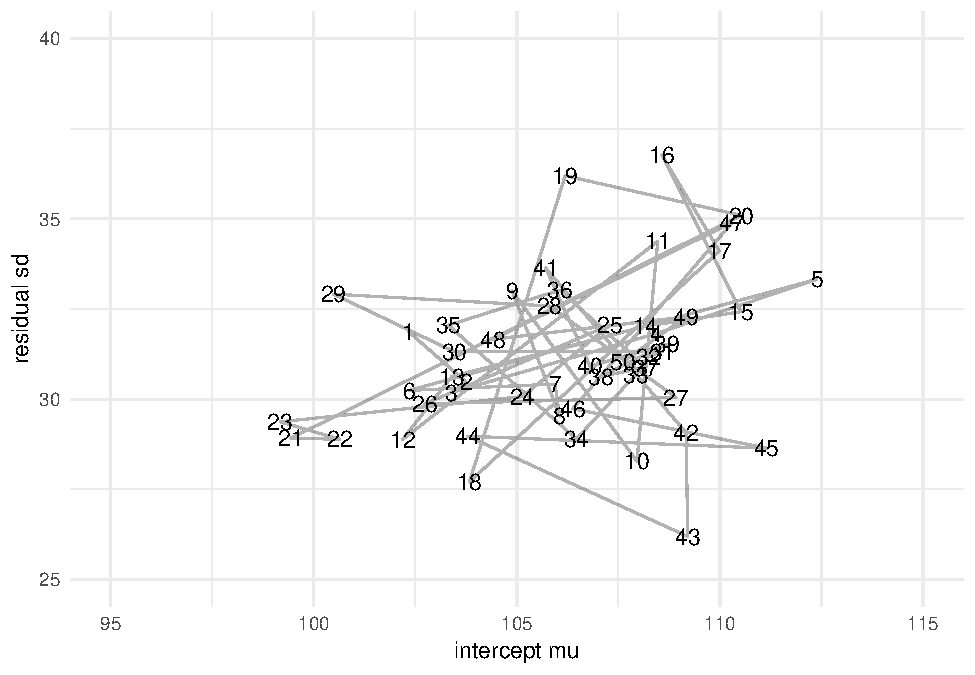
\includegraphics{Classic_linear_models_files/figure-latex/99_seconds_random_walk-1.pdf}

The more complex regression models grow, the more dimensions the PD
gets. The linear regression model in the next chapter has a three
parameter dimensions, which is difficult to visualize. Multi-level
models have hundreds of parameters, which is impossible to
intellectually grasp at once. Therefore, it is common to use the
\emph{marginal posterior distributions} (MPD), which give the density of
one coefficient at time. My preferred geometry for plotting MPDs is the
violin plot, which packs a bunch of densities and therefore can be used
for models of higher dimension. Still, for simple models histograms do
the job:

\begin{Shaded}
\begin{Highlighting}[]
\NormalTok{P_}\DecValTok{1} \OperatorTok\StringTok{ }
\StringTok{  }\KeywordTok{ggplot}\NormalTok{(}\KeywordTok{aes}\NormalTok{(}\DataTypeTok{x =}\NormalTok{ value)) }\OperatorTok{+}
\StringTok{  }\KeywordTok{geom_histogram}\NormalTok{() }\OperatorTok{+}
\StringTok{  }\KeywordTok{facet_grid}\NormalTok{(. }\OperatorTok{~}\StringTok{ }\NormalTok{parameter, }\DataTypeTok{scales =} \StringTok{"free"}\NormalTok{)}
\end{Highlighting}
\end{Shaded}

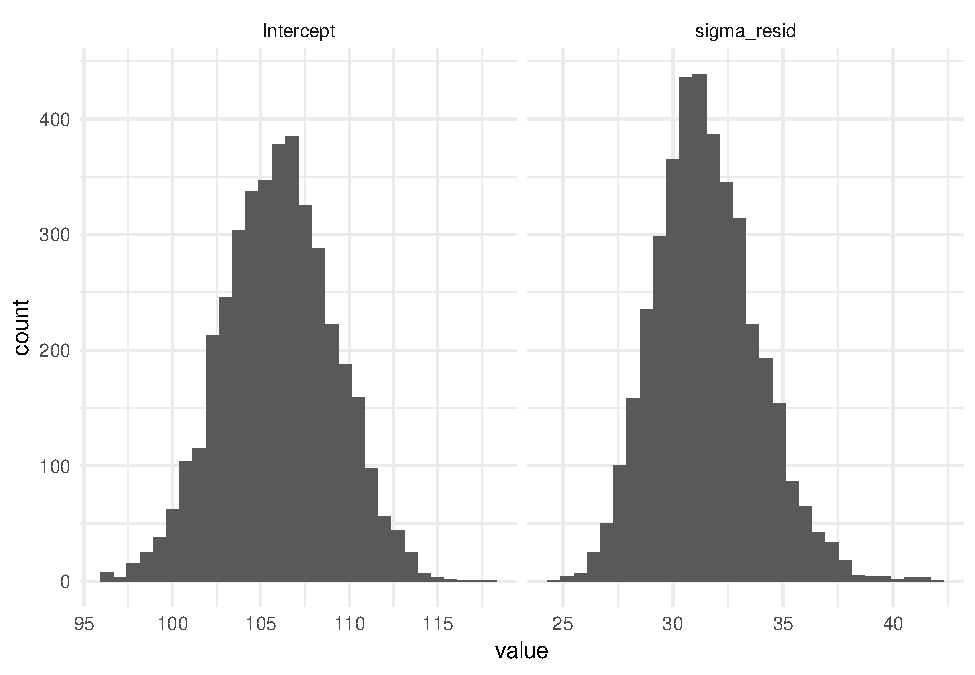
\includegraphics{Classic_linear_models_files/figure-latex/99_seconds_post-1.pdf}

In our example, in @ref(99\_seconds\_post) we can spot that the most
likely value for average time-on-task is \(106.1\). Both distributions
have a certain spread. With a wider PD, far-off values have been visited
by the MCMC chain more frequently. The probability mass is more evenly
distributed and there is less certainty for the parameter to fall in the
central region. In the current case, a risk averse decision maker would
maybe take the credibility interval as ``reasonably certain''.

Andrew and Jane expect some scepticism from the marketing people, and
some lack in statistical skills, too. What would be the most
comprehensible single number to report? As critical decisions are
involved, it seems plausible to report the risk to err: how certain are
they that the true value is more than 99 seconds. We inspect the
histograms. The MPD of the intercept indicates that the average
time-on-task is rather unlikely in the range of 99 seconds or better.
But what is the precise probability to err for the 99 seconds statement?
The above summary with \texttt{fixef()} does not answer the question,
accurately. The CI gives lower and upper limits for a range of 95\%
certainty in total. What is needed is the certainty of \(\mu \geq 99\).
Specific questions deserve precise answers. And once we have understood
the MCMC chain as a frequency distribution, the answer is easy: we
simply count how many visited values are larger than 99. In R, the
\texttt{quantile} function handles the job:

\begin{Shaded}
\begin{Highlighting}[]
\NormalTok{T_certainty <-}
\StringTok{  }\NormalTok{P_}\DecValTok{1} \OperatorTok\StringTok{ }
\StringTok{  }\KeywordTok{filter}\NormalTok{(parameter }\OperatorTok{==}\StringTok{ "Intercept"}\NormalTok{) }\OperatorTok
\StringTok{  }\KeywordTok{summarize}\NormalTok{(}\DataTypeTok{certainty_99s =} \KeywordTok{mean}\NormalTok{(value }\OperatorTok{>=}\StringTok{ }\DecValTok{99}\NormalTok{),}
            \DataTypeTok{certainty_111s =} \KeywordTok{mean}\NormalTok{(value }\OperatorTok{>=}\StringTok{ }\DecValTok{111}\NormalTok{))}

\KeywordTok{kable}\NormalTok{(T_certainty)}
\end{Highlighting}
\end{Shaded}

\begin{tabular}{r|r}
\hline
certainty\_99s & certainty\_111s\\
\hline
0.986 & 0.054\\
\hline
\end{tabular}

It turns out that the certainty for average time-on-task above the 99 is
an overwhelming 0.986. The alternative claim, that average completion
time is better than 111 seconds, has a rather moderate risk to err
(0.054).

\begin{Shaded}
\begin{Highlighting}[]
\KeywordTok{detach}\NormalTok{(Sec99)}
\end{Highlighting}
\end{Shaded}

\section{Walk the line: linear regression}\label{linear-regression}

In the previous section we have introduced the mother of all regression
models: the grand mean model. It assigns rather coarse predictions,
without any real predictors. Routinely, design researchers desire to
predict performance based on \emph{metric variables}, such as:

\begin{itemize}
\tightlist
\item
  previous experience
\item
  age
\item
  font size
\item
  intelligence level and other innate abilities
\item
  level of self efficiacy, neuroticism or other traits
\item
  number of social media contacts
\end{itemize}

To carry out such a research question, the variable of interest needs to
be measured, next to the outcome variable. And, the variable must vary.
You cannot examine the effects of age of font size on reading
performance, when all participants are psychology students or you test
only one size. Then, for specifying the model, the researcher has to
come up with an expectation of how the two are related. Theoretically,
that can be any mathematical function, but practically, a \emph{linear
function} is often presumed for its simplicity. The following plot shows
a variety of linear relations between two variables \(x\) and \(y\).

\begin{Shaded}
\begin{Highlighting}[]
\NormalTok{mascutils}\OperatorTok{::}\KeywordTok{expand_grid}\NormalTok{(}\DataTypeTok{intercept =} \KeywordTok{c}\NormalTok{(}\DecValTok{0}\NormalTok{, }\DecValTok{1}\NormalTok{, }\DecValTok{2}\NormalTok{),}
                       \DataTypeTok{slope =} \KeywordTok{c}\NormalTok{(}\OperatorTok{-}\NormalTok{.}\DecValTok{5}\NormalTok{, }\DecValTok{0}\NormalTok{, }\FloatTok{1.5}\NormalTok{),}
                       \DataTypeTok{x =} \OperatorTok{-}\DecValTok{3}\OperatorTok{:}\DecValTok{3}\NormalTok{) }\OperatorTok
\StringTok{  }\KeywordTok{arrange}\NormalTok{(x) }\OperatorTok\StringTok{ }
\StringTok{  }\KeywordTok{mutate}\NormalTok{(}\DataTypeTok{y =}\NormalTok{ intercept }\OperatorTok{+}\StringTok{ }\NormalTok{x }\OperatorTok{*}\StringTok{ }\NormalTok{slope,}
         \DataTypeTok{slope =} \KeywordTok{as.factor}\NormalTok{(slope)) }\OperatorTok\StringTok{ }
\StringTok{  }\KeywordTok{ggplot}\NormalTok{(}\KeywordTok{aes}\NormalTok{(}\DataTypeTok{x =}\NormalTok{ x, }\DataTypeTok{y =}\NormalTok{ y, }\DataTypeTok{color =}\NormalTok{ slope)) }\OperatorTok{+}
\StringTok{  }\KeywordTok{geom_line}\NormalTok{() }\OperatorTok{+}
\StringTok{  }\KeywordTok{facet_grid}\NormalTok{(}\OperatorTok{~}\NormalTok{intercept)}
\end{Highlighting}
\end{Shaded}

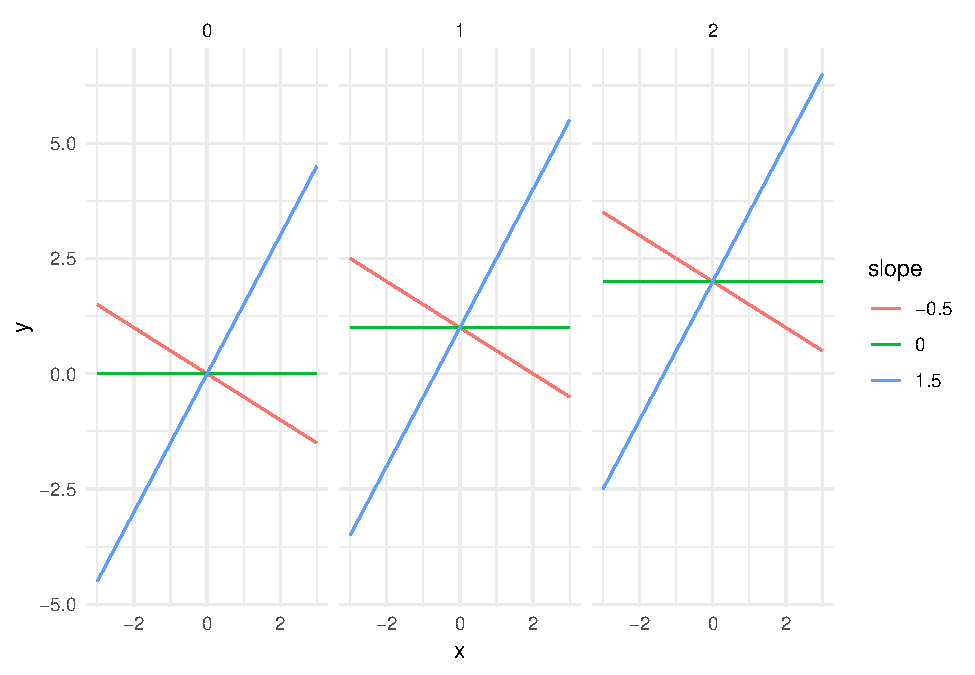
\includegraphics{Classic_linear_models_files/figure-latex/unnamed-chunk-12-1.pdf}

A linear function is a straight line, which is specified by two
parameters: \emph{intercept} \(\beta_0\) and \emph{slope} \(\beta_1\):
\[f(x_1) = \beta_0 + \beta_1x_{1i}\] The intercept is \emph{``the point
where a function graph crosses the x-axis''}, or more formally:

\[f(x_1 = 0) = \beta_0\]

The second parameter, \(\beta_1\) is called the \emph{slope}. The slope
determines the steepness of the line. When the slope is \(1\), the line
will raise by this amount when one moves one step to the right.

\[f(x_1 + 1) = \beta_0 + \beta_1x_{1i} + \beta_1\]

There is also the possibility that the slope is zero. In such a case,
the predictor has no effect and can be left out. Setting \(\beta_1 = 0\)
produces a horizontal line, with \(y\) being constant over the whole
range. This shows that The LRM can be conceived a generalization of the
GM model: \(\mu_i = \beta_0\).

Linear regression gives us the opportunity to discover how ToT can be
predicted by age (\(x_1\)) in the BrowsingAB case. IN this synthetic
experiment, two designs A and B are compared, but this is what we ignore
for now. Instead, we ask: are older people slower on the internet? or:
is there a linear relationship between age and ToT? The likelihood and
random terms of the LRM are:

\[\mu_i = \beta_0 + \beta_1x_{1i}\] \[Y_i = N(\mu_i, \sigma)\]

This literally means: with every year of age, ToT increases by the
\(\beta_1\) seconds. Before we run a linear regression with
\texttt{stan\_glm}, we visually explore the association between age and
ToT using a scatter plot. The blue line in the graph is a so called a
\emph{smoother}, more specifically a LOESS. A smoother is an estimated
line, just as linear function. But, it is way more flexible. Where the
linear function is a lever fixed at a pivotal point, LOESS is a pipe
cleaner. LOESS shows a more detailed picture of the relation between age
and ToT. There is a rise between 20 and 40, followed by a stable
plateau, and another rise starting at 60. Actually, that does not look
like a straight line, but at least there is steady upwards trend.

\begin{Shaded}
\begin{Highlighting}[]
\KeywordTok{attach}\NormalTok{(BrowsingAB)}
\end{Highlighting}
\end{Shaded}

\begin{Shaded}
\begin{Highlighting}[]
\NormalTok{G_eda_}\DecValTok{1}\NormalTok{ <-}
\StringTok{  }\NormalTok{BAB1 }\OperatorTok
\StringTok{  }\KeywordTok{ggplot}\NormalTok{(}\KeywordTok{aes}\NormalTok{(}\DataTypeTok{x =}\NormalTok{ age, }\DataTypeTok{y =}\NormalTok{ ToT)) }\OperatorTok{+}
\StringTok{  }\KeywordTok{geom_point}\NormalTok{()}\OperatorTok{+}
\StringTok{  }\KeywordTok{geom_smooth}\NormalTok{(}\DataTypeTok{se =}\NormalTok{ F, }\DataTypeTok{fullrange =}\NormalTok{ F)}

\NormalTok{G_eda_}\DecValTok{1}
\end{Highlighting}
\end{Shaded}

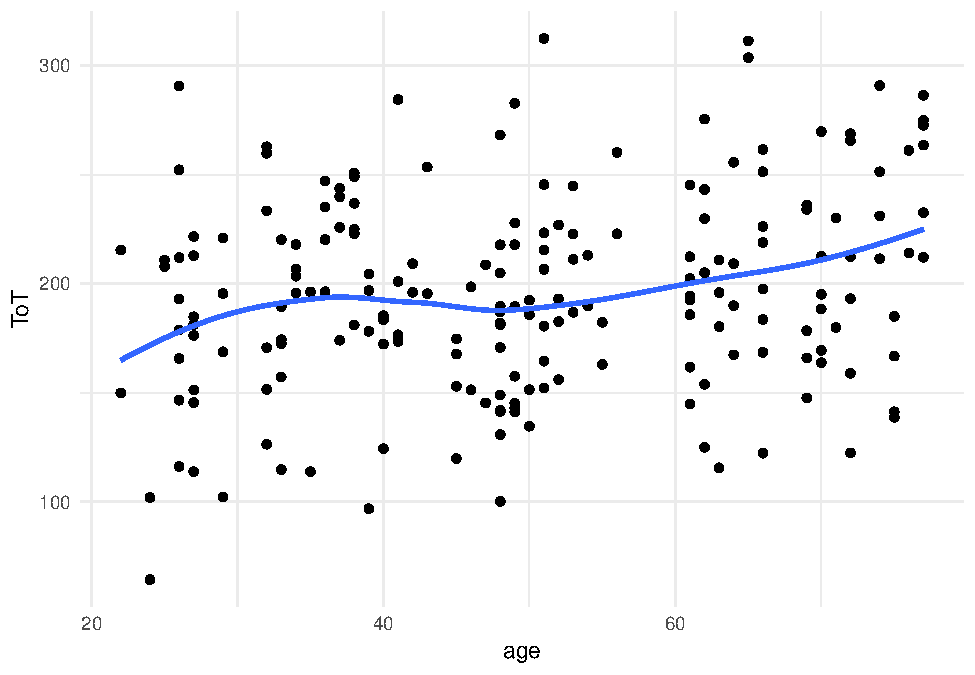
\includegraphics{Classic_linear_models_files/figure-latex/BAB_G_eda_1-1.pdf}

In fact, the BrowsingAB data contains what one could call a
psychological model. The effect of age is partly due to farsightedness
of participants (making them slower at reading), which more or less
suddenly kicks in at a certain range of age. Still, we currently make do
with a rough linear approximation. To estimate the model, we use the
\texttt{stan\_glm} command in much the same way as before, but add the
predictor age. The command will internally check the data type of your
variable, which is metric, here. Therefore, it is treated as a metric
predictor or \emph{covariate}.

\begin{Shaded}
\begin{Highlighting}[]
\NormalTok{M_age <-}
\StringTok{  }\NormalTok{BAB1 }\OperatorTok\StringTok{ }
\StringTok{  }\KeywordTok{stan_glm}\NormalTok{(ToT }\OperatorTok{~}\StringTok{ }\DecValTok{1} \OperatorTok{+}\StringTok{ }\NormalTok{age, }
           \DataTypeTok{data =}\NormalTok{ .)}
\end{Highlighting}
\end{Shaded}

\begin{Shaded}
\begin{Highlighting}[]
\NormalTok{T_age <-}\StringTok{ }\KeywordTok{fixef}\NormalTok{(M_age)}
\NormalTok{T_age}
\end{Highlighting}
\end{Shaded}

\begin{longtable}[]{@{}lrrr@{}}
\toprule
fixef & center & lower & upper\tabularnewline
\midrule
\endhead
Intercept & 164.090 & 143.152 & 185.18\tabularnewline
age & 0.642 & 0.234 & 1.04\tabularnewline
\bottomrule
\end{longtable}

Is age associated with ToT? The coefficient table tells us that with
every year of age, users get \(0.64\) seconds slower, which is
considerable. It also tells us that the predicted performance at age = 0
is \(164.09\).

\subsection{Transforming variables}\label{transforming-variables}

The intercept parameter refers to the predicted ToT of a new born. That
is a bizarre prediction and we would never seriously put that forward in
a stakeholder presentation, or in the conclusion of a scientific paper,
would we not? Besides that, the intercept estimate is rather uncertain,
with a wide 95\% interval, \(164.09 [143.15, 185.18]_{CI95}\).

Both, implausibility and high certainty are rooted in the same problem:
the model puts a parameter, where there is no data. The broad region of
the intercept is as empty as the Khali desert, because observations are
impossible or have not been recorded. Fortunately, there is a pragmatic
solution to the problem: \emph{shifting the predictor}. ``Shifting''
literally means that the age predictor is moved to the right or the
left, such that the zero point is in a region populated with
observations. In the case, here, two options seem to make sense: either,
the intercept is in the region of youngest participants, or it is the
sample average, which is then called \emph{centering}. To shift a
variable, just subtract the amount of units (years) where you want the
intercept to be. Figure XY shows a shift of -20 and a centering shift on
the original variable age

\begin{Shaded}
\begin{Highlighting}[]
\NormalTok{BAB1 <-}
\StringTok{  }\NormalTok{BAB1 }\OperatorTok\StringTok{ }
\StringTok{  }\KeywordTok{mutate}\NormalTok{(}\DataTypeTok{age_shft =}\NormalTok{ age }\OperatorTok{-}\StringTok{ }\DecValTok{20}\NormalTok{,}
         \DataTypeTok{age_cntr =}\NormalTok{ age }\OperatorTok{-}\StringTok{ }\KeywordTok{mean}\NormalTok{(age))}

\NormalTok{BAB1 }\OperatorTok\StringTok{ }
\StringTok{  }\NormalTok{tidyr}\OperatorTok{::}\KeywordTok{gather}\NormalTok{(}\StringTok{"predictor"}\NormalTok{, }\StringTok{"age"}\NormalTok{, }\KeywordTok{starts_with}\NormalTok{(}\StringTok{"age"}\NormalTok{)) }\OperatorTok\StringTok{ }
\StringTok{  }\KeywordTok{ggplot}\NormalTok{(}\KeywordTok{aes}\NormalTok{(}\DataTypeTok{x =}\NormalTok{ age, }\DataTypeTok{y =}\NormalTok{ ToT)) }\OperatorTok{+}
\StringTok{  }\KeywordTok{facet_grid}\NormalTok{(predictor}\OperatorTok{~}\NormalTok{.) }\OperatorTok{+}
\StringTok{  }\KeywordTok{geom_point}\NormalTok{() }\OperatorTok{+}
\StringTok{  }\KeywordTok{geom_smooth}\NormalTok{(}\DataTypeTok{se =}\NormalTok{ F, }\DataTypeTok{method =} \StringTok{"lm"}\NormalTok{, }\DataTypeTok{fullrange =}\NormalTok{ T)}
\end{Highlighting}
\end{Shaded}

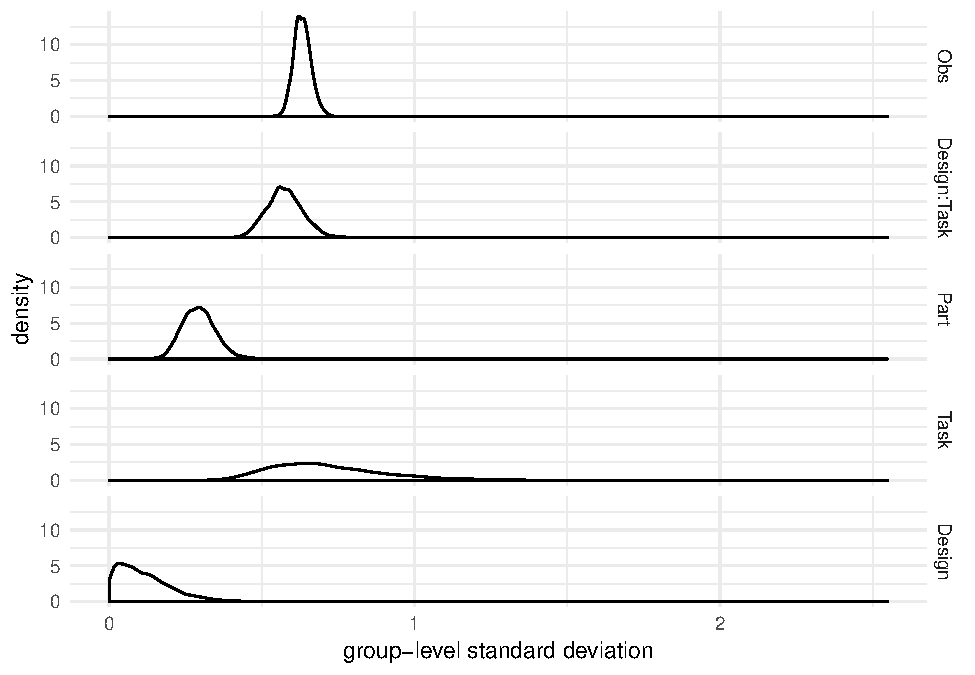
\includegraphics{Classic_linear_models_files/figure-latex/unnamed-chunk-15-1.pdf}

By shifting the age variable, the whole data cloud is moved to the left.
To see what happens on the inferential level, we repeat the LRM
estimation with the two shifted variables:

\begin{Shaded}
\begin{Highlighting}[]
\NormalTok{M_age_shft <-}\StringTok{ }
\StringTok{  }\KeywordTok{stan_glm}\NormalTok{(ToT }\OperatorTok{~}\StringTok{ }\DecValTok{1} \OperatorTok{+}\StringTok{ }\NormalTok{age_shft, }\DataTypeTok{data =}\NormalTok{ BAB1)}

\NormalTok{M_age_cntr <-}\StringTok{ }
\StringTok{  }\KeywordTok{stan_glm}\NormalTok{(ToT }\OperatorTok{~}\StringTok{ }\DecValTok{1} \OperatorTok{+}\StringTok{ }\NormalTok{age_cntr, }\DataTypeTok{data =}\NormalTok{ BAB1)}
\end{Highlighting}
\end{Shaded}

We combine the posterior distributions into one multi-model posterior
and read the \emph{multi-model coefficient table}:

\begin{Shaded}
\begin{Highlighting}[]
\NormalTok{P_age <-}\StringTok{ }
\StringTok{  }\KeywordTok{bind_rows}\NormalTok{(}\KeywordTok{posterior}\NormalTok{(M_age), }
            \KeywordTok{posterior}\NormalTok{(M_age_shft), }
            \KeywordTok{posterior}\NormalTok{(M_age_cntr))}


\NormalTok{T_age <-}\StringTok{ }\KeywordTok{fixef}\NormalTok{(P_age)}
\NormalTok{T_age}
\end{Highlighting}
\end{Shaded}

\begin{longtable}[]{@{}llrrr@{}}
\toprule
model & fixef & center & lower & upper\tabularnewline
\midrule
\endhead
M\_age & Intercept & 164.090 & 143.152 & 185.18\tabularnewline
M\_age & age & 0.642 & 0.234 & 1.04\tabularnewline
M\_age\_cntr & Intercept & 195.888 & 189.843 & 202.09\tabularnewline
M\_age\_cntr & age\_cntr & 0.641 & 0.265 & 1.05\tabularnewline
M\_age\_shft & Intercept & 176.688 & 163.262 & 190.25\tabularnewline
M\_age\_shft & age\_shft & 0.645 & 0.256 & 1.04\tabularnewline
\bottomrule
\end{longtable}

When comparing the regression results The shifted intercepts have moved
to higher values, as expected. Surprisingly, the simple shift is not
exactly 20 years. This is due to the high uncertainty of the first
model, as well as the relation not being exactly linear (see Figure XY).
The shifted age predictor has a slightly better uncertainty, but not by
much. This is, because the region around the lowest age is scarcely
populated with data for the very reason. Centering on the other hand
results in a highly certain estimate, no surprisingly, as the region is
densily populated. At the same time, the slope parameter practically
does not change, neither in magnitude nor in certainty.

An even stronger standardization is \emph{z-transformation}, where the
predictor is centered at zero and all values are divided by the standard
deviation, which results in a change of spread:

\begin{Shaded}
\begin{Highlighting}[]
\NormalTok{BAB1 <-}
\StringTok{  }\NormalTok{BAB1 }\OperatorTok\StringTok{ }
\StringTok{  }\KeywordTok{mutate}\NormalTok{(}\DataTypeTok{age_z =}\NormalTok{ (age }\OperatorTok{-}\StringTok{ }\KeywordTok{mean}\NormalTok{(age))}\OperatorTok{/}\KeywordTok{sd}\NormalTok{(age),}
         \DataTypeTok{age_cntr =}\NormalTok{ age }\OperatorTok{-}\StringTok{ }\KeywordTok{mean}\NormalTok{(age))}

\NormalTok{BAB1 }\OperatorTok\StringTok{ }
\StringTok{  }\NormalTok{tidyr}\OperatorTok{::}\KeywordTok{gather}\NormalTok{(}\StringTok{"predictor"}\NormalTok{, }\StringTok{"age"}\NormalTok{, age, age_z) }\OperatorTok\StringTok{ }
\StringTok{  }\KeywordTok{ggplot}\NormalTok{(}\KeywordTok{aes}\NormalTok{(}\DataTypeTok{x =}\NormalTok{ age, }\DataTypeTok{y =}\NormalTok{ ToT)) }\OperatorTok{+}
\StringTok{  }\KeywordTok{facet_grid}\NormalTok{(predictor}\OperatorTok{~}\NormalTok{.) }\OperatorTok{+}
\StringTok{  }\KeywordTok{geom_point}\NormalTok{() }\OperatorTok{+}
\StringTok{  }\KeywordTok{geom_smooth}\NormalTok{(}\DataTypeTok{se =}\NormalTok{ F, }\DataTypeTok{method =} \StringTok{"lm"}\NormalTok{, }\DataTypeTok{fullrange =}\NormalTok{ T)}
\end{Highlighting}
\end{Shaded}

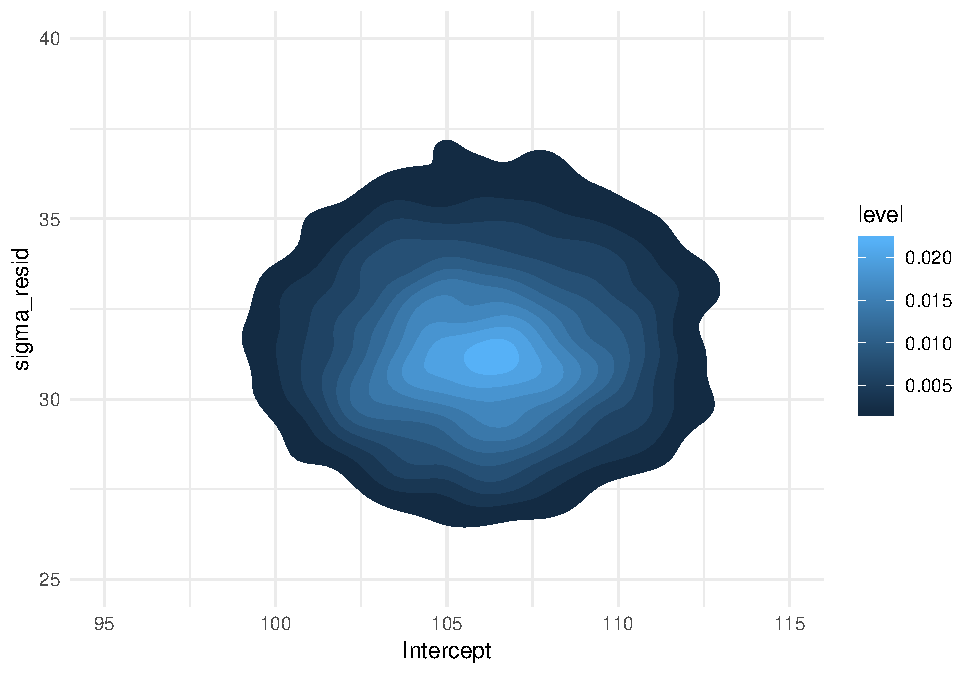
\includegraphics{Classic_linear_models_files/figure-latex/unnamed-chunk-19-1.pdf}

A z-transformed variable is centered on zero and has a standard
deviation of one. As can be seen, z-transformation has a considerable
effect on the slope. Pulling the data cloud together pulls up the slope.
Again, we run an LRM and compare against the original model:

\begin{Shaded}
\begin{Highlighting}[]
\NormalTok{M_age_z <-}\StringTok{ }
\StringTok{  }\KeywordTok{stan_glm}\NormalTok{(ToT }\OperatorTok{~}\StringTok{ }\DecValTok{1} \OperatorTok{+}\StringTok{ }\NormalTok{age_z, }\DataTypeTok{data =}\NormalTok{ BAB1)}
\end{Highlighting}
\end{Shaded}

\begin{Shaded}
\begin{Highlighting}[]
\NormalTok{P_age <-}\StringTok{  }\KeywordTok{bind_rows}\NormalTok{(P_age, }\KeywordTok{posterior}\NormalTok{(M_age_z))}
\NormalTok{T_age <-}\StringTok{ }\KeywordTok{fixef}\NormalTok{(P_age)}
\NormalTok{T_age}
\end{Highlighting}
\end{Shaded}

\begin{longtable}[]{@{}llrrr@{}}
\toprule
model & fixef & center & lower & upper\tabularnewline
\midrule
\endhead
M\_age & Intercept & 164.090 & 143.152 & 185.18\tabularnewline
M\_age & age & 0.642 & 0.234 & 1.04\tabularnewline
M\_age\_cntr & Intercept & 195.888 & 189.843 & 202.09\tabularnewline
M\_age\_cntr & age\_cntr & 0.641 & 0.265 & 1.05\tabularnewline
M\_age\_shft & Intercept & 176.688 & 163.262 & 190.25\tabularnewline
M\_age\_shft & age\_shft & 0.645 & 0.256 & 1.04\tabularnewline
M\_age\_z & Intercept & 195.873 & 189.852 & 202.37\tabularnewline
M\_age\_z & age\_z & 10.118 & 3.720 & 16.24\tabularnewline
\bottomrule
\end{longtable}

As expected, the intercept matches that of the centered variable. The
small deviations are due to the {[}random walk{]} (\#random\_walk) and
disappear when running longer MCMC chains. The slope parameter has
inflated dramatically. That, of course, is not a magical trick to obtain
more impressive numbers, it is simply the effect of dividing the
original variable by its standard deviation. A step of one on
\texttt{age} is exactly one year, whereas in \texttt{age\_z} it is
\emph{one standard deviation}. Z-transformation adjusts a variable by
its observed dispersion, measured as standard deviations. In the case of
age, this is not very desirable.

Years of age is a natural and commonly understood unit and my advice
would be to use centering, leaving the unit size untouched. When dealing
with variables that are pseudo-metric, rating scales in particular,
z-transformation makes sense. Imagine you were stranded on a tropical
island. While putting together a shelter, you realize of useful a meter
stick is. The \emph{ur meter} is thousands of kilometers away.
Obviously, you can bootstrap yourself by picking up a reasoable straight
stick and mark 10 (or eight) equally spaced sections. With
z-transformation you are picking your unit of measurment on what you
find, too. Still, ``one standard deviation'' is hard to swallow for
anyone untrained. If we can assume the measurement to be normally
distributed, which is frequently a good approximation for rating scale
data, we can derive relative statements. As it happens, the central two
standard deviations cover around two thirds of the full area, leaving
one sixth to each tail. That allows to make quantile statements, such
as: Within central two thirds regarding age, ToT moves up by
\(2 \beta_1 = 10.12\) seconds, if age is truly Normal, of course.

A general useful application of z-scores is to bootstrap a common unit
for a diverse set of measures. Think of a battery of Likert scales, that
all choose their own ranges. With z-scores we can compare the relative
impact of several predictors in a population. In fact, that even makes
sense for the age model. As it happens, the random variation parameter
\(\sigma\) is given in standard deviation units, too. We can conclude
that the age effect causes just a moderate fraction of all the variation
observed. More research is needed.

\subsection{Correlations}\label{correlations}

LRM render the relationship between two metric variables. A commonly
known statistic that seems to do the same is Pearson's correlation
coefficient \(r\) (@\ref(\#associations)). In the following, we will see
that a tight connection between correlation and linear coefficients
exists, albeit both having their own advantages. For a demonstration, we
reproduce the steps on a smimulated data set where X and Y are linearly
linked:

\begin{Shaded}
\begin{Highlighting}[]
\NormalTok{D_cor <-}
\StringTok{  }\KeywordTok{data_frame}\NormalTok{(}\DataTypeTok{x =} \KeywordTok{runif}\NormalTok{(}\DecValTok{100}\NormalTok{, }\DecValTok{0}\NormalTok{, }\DecValTok{50}\NormalTok{),}
             \DataTypeTok{y =} \KeywordTok{rnorm}\NormalTok{(}\DecValTok{100}\NormalTok{, x }\OperatorTok{*}\NormalTok{.}\DecValTok{2}\NormalTok{, }\DecValTok{3}\NormalTok{))}
\end{Highlighting}
\end{Shaded}

\begin{Shaded}
\begin{Highlighting}[]
\NormalTok{D_cor }\OperatorTok\StringTok{ }
\StringTok{  }\KeywordTok{ggplot}\NormalTok{(}\KeywordTok{aes}\NormalTok{(}\DataTypeTok{x =}\NormalTok{ x, }\DataTypeTok{y =}\NormalTok{ y)) }\OperatorTok{+}
\StringTok{  }\KeywordTok{geom_point}\NormalTok{() }\OperatorTok{+}
\StringTok{  }\KeywordTok{geom_smooth}\NormalTok{(}\DataTypeTok{method =} \StringTok{"lm"}\NormalTok{, }\DataTypeTok{se =}\NormalTok{ F)}
\end{Highlighting}
\end{Shaded}

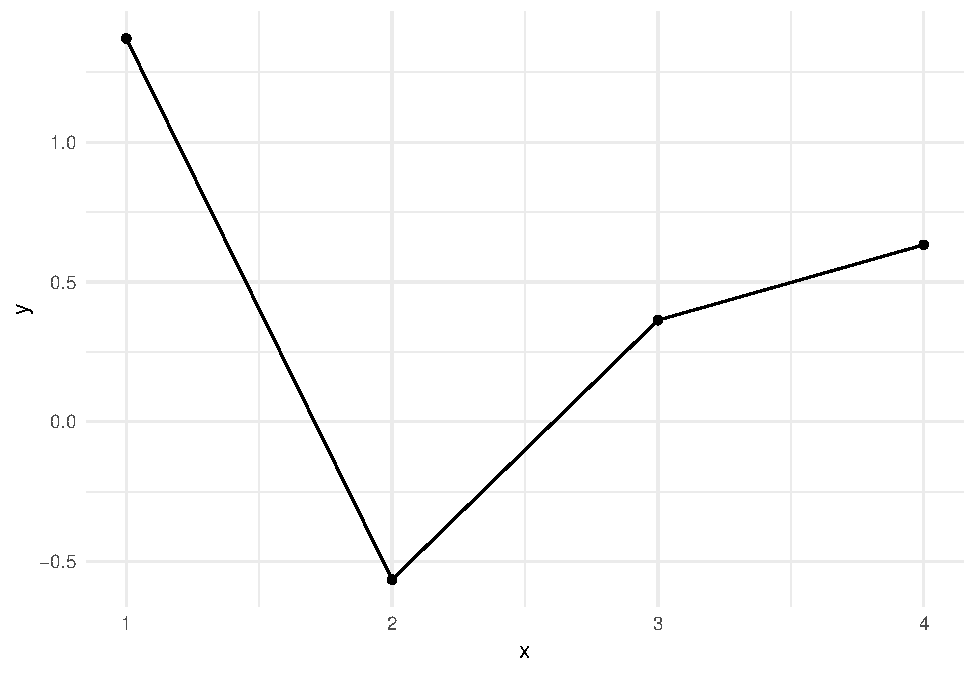
\includegraphics{Classic_linear_models_files/figure-latex/unnamed-chunk-24-1.pdf}

Recall, that \(r\) is covariance standardized for dispersion and that a
covariance is the mean squared deviance from the population mean. This
is how the correlation coefficient is decontaminated from the
idiosyncracies of the involved measures, their location and dispersion.
In contrast, slope parameter in an LRM is a measure of association, too.
It is agnostic of the overall location of measures, because this is
captured by the intercept. However, dispersion remains intact. That
makes that slope and intercept together retain information about
location, dispersion and association of data and we can ultimately make
predictions. Still, there is a tight re.lationship between Pearson \(r\)
and a slope coefficient \(\beta_1\), namely:

\[
r = \beta_1 \frac{sd_X}{sd_Y}
\]

For the sole purpose of demonstration, we here resort to the built-in
non-Bayesian command \texttt{lm} for doing the regression.

\begin{Shaded}
\begin{Highlighting}[]
\NormalTok{M_cor <-}\StringTok{ }\KeywordTok{lm}\NormalTok{(y }\OperatorTok{~}\StringTok{ }\NormalTok{x, D_cor)}
\NormalTok{beta_}\DecValTok{1}\NormalTok{ <-}\StringTok{ }\NormalTok{stats}\OperatorTok{::}\KeywordTok{coef}\NormalTok{(M_cor)[}\DecValTok{2}\NormalTok{]}

\NormalTok{r <-}\StringTok{ }\NormalTok{beta_}\DecValTok{1} \OperatorTok{*}\StringTok{ }\KeywordTok{sd}\NormalTok{(D_cor}\OperatorTok{$}\NormalTok{x) }\OperatorTok{/}\StringTok{ }\KeywordTok{sd}\NormalTok{(D_cor}\OperatorTok{$}\NormalTok{y)}
\NormalTok{r}
\end{Highlighting}
\end{Shaded}

\begin{verbatim}
##     x 
## 0.707
\end{verbatim}

The clue with Pearson \(r\) is that it normalized the slope coefficient
by the variation found in the sample. This reminds of z-transformation
as was introduced in \ref{transforming-variables}. In fact, when both,
predictor and outcome, are z-transformed before estimation, the
coefficient equals Pearson's \(r\), right away:

\begin{Shaded}
\begin{Highlighting}[]
\NormalTok{M_z <-}
\StringTok{  }\NormalTok{D_cor }\OperatorTok\StringTok{ }
\StringTok{  }\KeywordTok{mutate}\NormalTok{(}\DataTypeTok{x_z =}\NormalTok{ (x }\OperatorTok{-}\StringTok{ }\KeywordTok{mean}\NormalTok{(x))}\OperatorTok{/}\KeywordTok{sd}\NormalTok{(x),}
         \DataTypeTok{y_z =}\NormalTok{ (y }\OperatorTok{-}\StringTok{ }\KeywordTok{mean}\NormalTok{(y))}\OperatorTok{/}\KeywordTok{sd}\NormalTok{(y)) }\OperatorTok\StringTok{ }
\StringTok{  }\KeywordTok{lm}\NormalTok{(y_z }\OperatorTok{~}\StringTok{ }\NormalTok{x_z, .)}

\NormalTok{stats}\OperatorTok{::}\KeywordTok{coef}\NormalTok{(M_z)[}\DecValTok{2}\NormalTok{]}
\end{Highlighting}
\end{Shaded}

\begin{verbatim}
##   x_z 
## 0.707
\end{verbatim}

In regression modelling the use of coefficients prevales because they
allow for predictions. However, correlation coefficients play a major
role in two situations: in exploratory data analysis and in multilevel
models. With the latter we will deal in @\ref(re\_correlations). For
exploratory data analysis it is recommended to inspect pairwise
correlations for the following reasons:

\begin{enumerate}
\def\labelenumi{\arabic{enumi}.}
\tightlist
\item
  Correlations between predictors and responses are a quick and dirty
  assessment of the expected associations
\item
  Correlations between multiple response modalities (e.g., ToT and
  number of errors) indicate to what extent these responses can be
  considered exchangeable.
\item
  Correlations between predictors should be checked upfront to avoid
  problems arising from so-called colinearity.
\end{enumerate}

\subsection{Endlessly linear}\label{endlessly-linear}

On a deeper level the bizarre age = 0 prediction is an example of a
principle, that will re-occur several times throughout this book.

\textbf{In an endless universe, everything is finite.}

A well understood fact about LRM is that they allow us to fit a straight
line to data. A lesser regarded consequence from the mathematical
underpinnings of such models is that this line extends infinitely in
both directions. To fulfill this assumption, the outcome variable needs
to have an infinite range, too, \(y_i \in [-infty; \infty]\) (unless the
slope is zero). Every scientifically trained person and many lay people
know, that even elementary magnitude in physics are finite: all speeds
are limited to \(\approx 300.000 km/s\), the speed of light and
temperature has a lower limit of -276°C (or 0K). If there can neither be
endless acceleration nor cold, it would be daring to assume any
psychological effect to be infinite in both directions.

The endlessly linear assumption (ELA) is a central piece of all LRM.
From a formal perspective, the ELA is always violated in a universe like
ours. So, should we never ever use a linear model and move on to
non-linear models right away? Pragmatically, the LRM often is a
reasonably effective approximation. From figure {[}G\_eda\_1{]} we have
seen that the increase is not strictly linear, but follows a more
complex curved pattern. This pattern might be of interest to someone
studying the psychological causes of the decline in performance. For the
applied design researcher it probably suffices to summarize the
monotonous relationship by the slope coefficient. In \ref{line-by-line}
we will estimate the age effects for designs A and B, separately, which
lets us compare fairness towards older people.

As has been said theorists may desire more detailed picture and see
disruptions of linearity as indicators for interesting psychological
processes. An uncanny example of theoretical work will be given in
polynomial regression. For the rest of us, linear regression is a
pragmatic choice, as long as:

\begin{enumerate}
\def\labelenumi{\arabic{enumi}.}
\tightlist
\item
  the pattern is monotonically increasing
\item
  any predictions stay in the observed range and avoid the boundary
  regions, or beyond.
\end{enumerate}

\subsection{Posterior predictions}\label{posterior-predictions}

In Bayesian regression models, \emph{posterior predictions} are a
simple, yet powerful concept to compare the fitted model with the
original data. As {[}McElreath{]} points out, one should rather call
them \emph{retrodictions}, because they regard the real data one has,
not the future. In yet another perspective they are \emph{idealized
responses} and as such address both, present and future. Posterior
predictions are routinely compared to \emph{observed values} \(y_i\)
which are known beforehand, but still contain the randomness component.
Fitting a linear model basically means separating the idealized effect
from the randomness. When the model is somewhat well-specified, this
succeeds but comes at the costs of uncertainty: the \emph{predicted
value is a random variable, too}.

In the BrowsingAB case, we have repeatedly recorded age of participant.
LRM found the repeating pattern, that with every unit of age, ToT
increased by 0.645 seconds. This pattern is what the model predicts, now
and forever. If we ask: what is predicted for a person of age 45? We get
the predicted value \(\mu_i\):

\[\mu_{age = 45} =176.688 + 0.645 * 45\\ 
= 205.707\]

The predicted value is our best guess under the LRM model. Like
coefficients, it is uncertain to some degree, but we are setting this
aside for the moment. What we know for sure is the \emph{observed value}
. A primitive procedure to get a best guess for someone of age 45 is to
find one matching case in the data and take this as face value. The data
set contains a few of those participants, but the situation is rather
scattered and the prediction is not clear.

\begin{Shaded}
\begin{Highlighting}[]
\NormalTok{BAB1 }\OperatorTok\StringTok{ }
\StringTok{  }\KeywordTok{select}\NormalTok{(Part, age, ToT) }\OperatorTok\StringTok{ }
\StringTok{  }\KeywordTok{filter}\NormalTok{(age }\OperatorTok{==}\StringTok{ }\DecValTok{45}\NormalTok{) }\OperatorTok\StringTok{ }
\StringTok{  }\KeywordTok{kable}\NormalTok{()}
\end{Highlighting}
\end{Shaded}

\begin{tabular}{r|r|r}
\hline
Part & age & ToT\\
\hline
28 & 45 & 153\\
\hline
68 & 45 & 168\\
\hline
128 & 45 & 120\\
\hline
168 & 45 & 175\\
\hline
\end{tabular}

A more disciplined way to obtain predicted values is to use the standard
command \texttt{predict} on the model object:

\begin{Shaded}
\begin{Highlighting}[]
\NormalTok{T_pred_age <-}
\StringTok{  }\NormalTok{BAB1 }\OperatorTok\StringTok{ }
\StringTok{  }\KeywordTok{select}\NormalTok{(Part, age, ToT) }\OperatorTok\StringTok{ }
\StringTok{  }\KeywordTok{mutate}\NormalTok{(}\DataTypeTok{mu =} \KeywordTok{predict}\NormalTok{(M_age_shft)}\OperatorTok{$}\NormalTok{center)}

\NormalTok{T_pred_age }\OperatorTok\StringTok{  }
\StringTok{  }\KeywordTok{filter}\NormalTok{(age }\OperatorTok{==}\StringTok{ }\DecValTok{45}\NormalTok{) }\OperatorTok\StringTok{ }
\StringTok{  }\KeywordTok{kable}\NormalTok{()}
\end{Highlighting}
\end{Shaded}

\begin{tabular}{r|r|r|r}
\hline
Part & age & ToT & mu\\
\hline
28 & 45 & 153 & 192\\
\hline
68 & 45 & 168 & 192\\
\hline
128 & 45 & 120 & 193\\
\hline
168 & 45 & 175 & 191\\
\hline
\end{tabular}

We see that all participants of age 45 get the same prediction. What
differs is the observed value, as this contains the influence of all
random sources at the time of measuring. We will return to residuals in
the next section.

What if we wanted to get a best guess for an age that did not occur in
our data set, say 43.5? Using the LR likelihood function above, we can
estimate the expectation for any value we want. By entering the
intercept and age estimates (\texttt{C\_age}), we obtain:

\begin{Shaded}
\begin{Highlighting}[]
\NormalTok{C_age <-}\StringTok{ }\KeywordTok{fixef}\NormalTok{(M_age_shft)}\OperatorTok{$}\NormalTok{center}
\NormalTok{C_age[}\DecValTok{1}\NormalTok{] }\OperatorTok{+}\StringTok{ }\FloatTok{43.5} \OperatorTok{*}\StringTok{ }\NormalTok{C_age[}\DecValTok{2}\NormalTok{]}
\end{Highlighting}
\end{Shaded}

\begin{verbatim}
## [1] 205
\end{verbatim}

With the same procedure, it is possible to plot observed and expected
values next to each other:

\begin{Shaded}
\begin{Highlighting}[]
\NormalTok{G_pred_age <-}
\StringTok{  }\NormalTok{BAB1 }\OperatorTok\StringTok{ }
\StringTok{  }\KeywordTok{ggplot}\NormalTok{(}\KeywordTok{aes}\NormalTok{(}\DataTypeTok{x =}\NormalTok{ age, }\DataTypeTok{y =}\NormalTok{ ToT)) }\OperatorTok{+}\StringTok{ }
\StringTok{  }\KeywordTok{geom_point}\NormalTok{() }\OperatorTok{+}
\StringTok{  }\KeywordTok{geom_abline}\NormalTok{(}\DataTypeTok{intercept =}\NormalTok{ C_age[}\DecValTok{1}\NormalTok{], }
              \DataTypeTok{slope =}\NormalTok{ C_age[}\DecValTok{2}\NormalTok{],}
              \DataTypeTok{col =} \StringTok{"red"}\NormalTok{)}

\NormalTok{G_pred_age}
\end{Highlighting}
\end{Shaded}

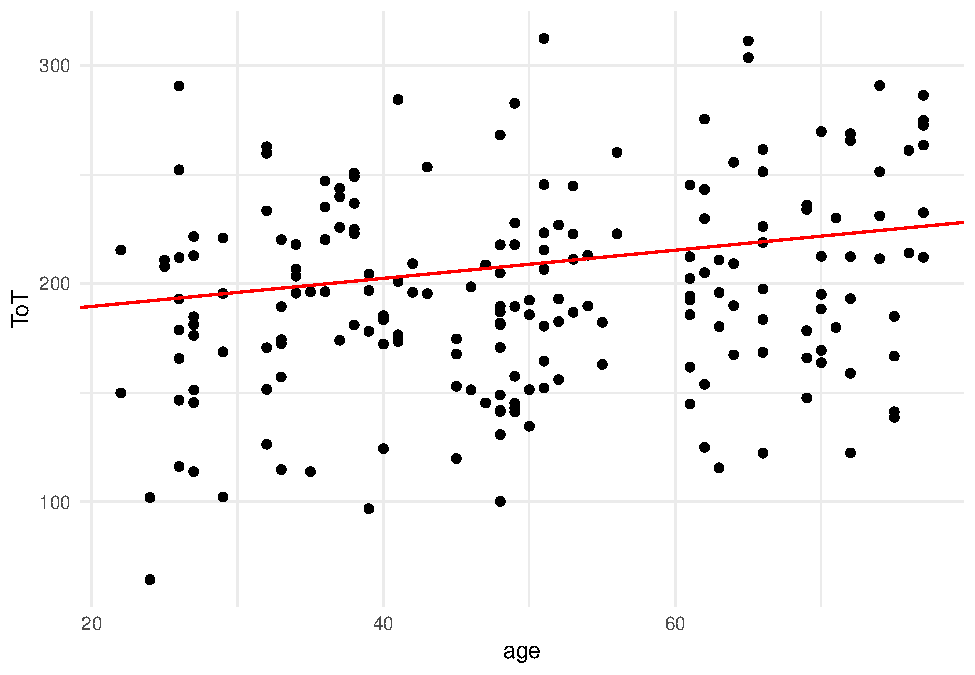
\includegraphics{Classic_linear_models_files/figure-latex/expected_values-1.pdf}

\begin{Shaded}
\begin{Highlighting}[]
\KeywordTok{detach}\NormalTok{(BrowsingAB)}
\end{Highlighting}
\end{Shaded}

This figure does not look too convincing. The regression line is rather
flat, indicating a small effect of age. In addition, it looks like a
lonely highway in a vast forest area. Just visually, a completely flat
line or a slight negative slope would be equally credible.

\begin{itemize}
\tightlist
\item
  resid-predict plots as a general form to discover trends
\item
  qq plots
\end{itemize}

\subsection{Exercises}\label{exercises-2}

\begin{enumerate}
\def\labelenumi{\arabic{enumi}.}
\item
  Examine the linear parameters of model \texttt{M\_age\_rtrn} and
  derive some impossible predictions, as was done in the previous
  section.
\item
  The BAB1 data set contains another outcome variable where the number
  of clicks was measured until the participant found the desired
  information. Specify a LR with age and examine the residual
  distribution. Is the Normality assumption reasonably defensible? What
  is the difference to home returns, despite both variables being
  counts?
\item
  Review the two figures in the first example of {[}GSR{]}. The
  observations are bi-modally distributed, nowhere near Gaussian. After
  (graphically) applying the model they are well-shaped. What does that
  tell you about checking residual assumptions before running the model?
\end{enumerate}

\section{A versus B: Comparison of groups}\label{CGM}

Another basic liknear model is the \emph{comparison of groups} (CGM),
which replaces the commonly known analysis of variance (ANOVA). In
design research group comparisons are all over the place, for example:

\begin{itemize}
\tightlist
\item
  comparing designs: as we have seen in the A/B testing scenario
\item
  comparing groups of people, like gender or whether they have a high
  school degree
\item
  comparing situations, like whether someone uses an app on the go, or
  sitting still behind a computer
\end{itemize}

In order to perform a CGM, a variable is needed that establishes the
groups. This is commonly called a \emph{factor}. A factor is a variable
that identifies members of groups, like ``A'' and ``B'' or ``male'' and
``female''. The groups are called \emph{factor levels}. In the
BrowsingAB case, the prominent factor is Design with its levels A and B.

Asking for differences between two (or more) designs is routine in
design research. For example, it could occur during an overhaul of a
municipal website. With the emerge of e-government, many municipal
websites have grown wildly over a decade. What once was a lean (but not
pretty) 1990 website over time has grown into a jungles, to the
disadvantage for the users. The BrowsingAB case could represent the
prototype of a novel web design, which is developed and tested via A/B
testing at 200 users. Every user is given the same task, but sees only
one of the two designs. The design team is interested in: \emph{do two
web designs A and B differ in user performance?}

Again, we first take a look at the raw data:

\begin{Shaded}
\begin{Highlighting}[]
\KeywordTok{attach}\NormalTok{(BrowsingAB)}
\end{Highlighting}
\end{Shaded}

\begin{Shaded}
\begin{Highlighting}[]
\NormalTok{BAB1 }\OperatorTok
\StringTok{  }\KeywordTok{ggplot}\NormalTok{(}\KeywordTok{aes}\NormalTok{(}\DataTypeTok{x =}\NormalTok{ ToT)) }\OperatorTok{+}
\StringTok{  }\KeywordTok{geom_histogram}\NormalTok{() }\OperatorTok{+}
\StringTok{    }\KeywordTok{facet_grid}\NormalTok{(Design}\OperatorTok{~}\NormalTok{.)}
\end{Highlighting}
\end{Shaded}

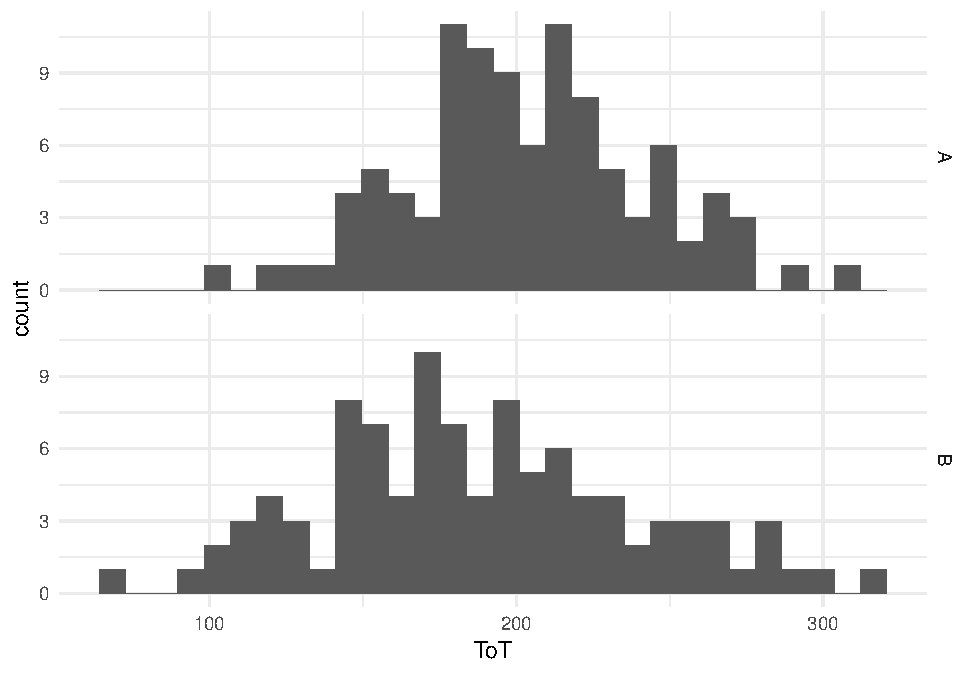
\includegraphics{Classic_linear_models_files/figure-latex/eda_anova-1.pdf}

This doesn't look too striking. We might consider a slight advantage for
design B, but the overlap is immense. We perform the CGM. Again, this is
a two-step procedure:

\begin{enumerate}
\def\labelenumi{\arabic{enumi}.}
\tightlist
\item
  the \texttt{stan\_glm} command lets you specify a simple formula to
  express the dependency between predictors (education) and outcome
  variable (ToT). It performs the parameter estimation, using the method
  of \emph{Markov-Chain Monte-Carlo Sampling}. The results are stored in
  a new object \texttt{M\_Design}.
\item
  With the \texttt{fixef} command the estimates are extracted and
  interpreted
\end{enumerate}

\begin{Shaded}
\begin{Highlighting}[]
\NormalTok{M_Design <-}
\StringTok{  }\NormalTok{BAB1 }\OperatorTok\StringTok{ }
\StringTok{  }\KeywordTok{stan_glm}\NormalTok{(ToT }\OperatorTok{~}\StringTok{ }\DecValTok{1} \OperatorTok{+}\StringTok{ }\NormalTok{Design, }
           \DataTypeTok{data =}\NormalTok{ .)}
\end{Highlighting}
\end{Shaded}

\begin{Shaded}
\begin{Highlighting}[]
\NormalTok{T_Design <-}\StringTok{ }\KeywordTok{fixef}\NormalTok{(M_Design)}
\NormalTok{T_Design}
\end{Highlighting}
\end{Shaded}

\begin{longtable}[]{@{}lrrr@{}}
\toprule
fixef & center & lower & upper\tabularnewline
\midrule
\endhead
Intercept & 203 & 194.7 & 212.21\tabularnewline
DesignB & -15 & -27.4 & -3.05\tabularnewline
\bottomrule
\end{longtable}

\begin{Shaded}
\begin{Highlighting}[]
\KeywordTok{detach}\NormalTok{(BrowsingAB)}
\end{Highlighting}
\end{Shaded}

The model contains two parameters, the first one being the
\emph{intercept}, again. How can you have a ``crossing point zero'',
when there is no line, but just two groups. You can't. When speaking of
pure factor models, like the one above or the multifactorial models of
the next section, the intercept has a different meaning, it is the
\emph{mean of a reference group}. Per default, stan\_glm chooses the
alphabetically first group label as the reference group, design A. We
can therefore say that design A has an average performance of
\(203.36 [194.7, 212.21]_{CI95}\).

The second parameter is the effect of ``moving to design B''. It is
given as the \emph{difference to the reference group}. With design B it
took users \(15.02 [27.36, 3.05]_{CI95}\) less time to complete the
task. This effect appears rather small and there is huge uncertainty
about it. It barely justifies the effort to replace design A with B. If
the BrowsingAB data set has some exciting stories to tell, the design
difference is not it.

\subsection{Not stupid: dummy variables}\label{dummy_variables}

Are we missing something so far? We have not seen the model formula,
yet. The CGM is a linear model, but this is not so apparent as it
contains a factor, a non-metric variable. Linear model terms are a sum
of products \(\beta_ix_i\), but factors cannot just enter such a term.
What would be the result of \(\mathrm{DesignB} \times\beta_1\)?

\emph{Factors} basically answer the question: \emph{What group does the
observation belong to?}. This is a label, not a number, and cannot enter
the regression formula. \emph{Dummy variables} solve the dilemma by
converzing factor levels to numbers. A dumma variable represents only
one level of a factor, by asking the simple question: \emph{Does this
observation belong to group DesignB?} The answer is yes/no and can be
coded by a Boolean variable. For every level, a separate dummy variable
is constructed to answer the simple yes/no question of membership. But,
can Boolean variables enter arithmetic equations? At least, R assumes
that this is safe, as they can always be converted to ones and zeros
using \texttt{as.numeric}. Routinely, we can leave the whole dummy
variable business to the linear model engine. Still, it is instructive
to do it yourself once.

\begin{Shaded}
\begin{Highlighting}[]
\KeywordTok{attach}\NormalTok{(BrowsingAB)}
\end{Highlighting}
\end{Shaded}

\begin{Shaded}
\begin{Highlighting}[]
\NormalTok{BAB1 <-}\StringTok{  }\NormalTok{BAB1 }\OperatorTok\StringTok{ }
\StringTok{  }\KeywordTok{mutate}\NormalTok{(}\DataTypeTok{d_A =} \KeywordTok{as.numeric}\NormalTok{(Design }\OperatorTok{==}\StringTok{ "A"}\NormalTok{),}
         \DataTypeTok{d_B =} \KeywordTok{as.numeric}\NormalTok{((Design }\OperatorTok{==}\StringTok{ "B"}\NormalTok{)))}
\NormalTok{BAB1 }\OperatorTok\StringTok{ }
\StringTok{  }\KeywordTok{select}\NormalTok{(Obs, Design, d_A, d_B, ToT) }\OperatorTok\StringTok{ }
\StringTok{  }\KeywordTok{sample_n}\NormalTok{(}\DecValTok{8}\NormalTok{) }\OperatorTok\StringTok{ }
\StringTok{  }\KeywordTok{kable}\NormalTok{()}
\end{Highlighting}
\end{Shaded}

\begin{tabular}{r|l|r|r|r}
\hline
Obs & Design & d\_A & d\_B & ToT\\
\hline
39 & A & 1 & 0 & 230\\
\hline
151 & B & 0 & 1 & 152\\
\hline
107 & B & 0 & 1 & 122\\
\hline
194 & B & 0 & 1 & 169\\
\hline
1 & A & 1 & 0 & 190\\
\hline
90 & A & 1 & 0 & 193\\
\hline
132 & B & 0 & 1 & 203\\
\hline
55 & A & 1 & 0 & 186\\
\hline
\end{tabular}

Vice versa, numbers in a logical context are always interpreted in
complete reverse.

\[ 
v = 1 \mapsto \mathrm{TRUE}\\ v = 0 \mapsto \mathrm{FALSE} 
\]

Boolean variables can be used in all contexts, including numerical and
categorical. It is unfortunate that we call them dummies in such a
belittling manner, as they are truly bridges between the world of
categories and arithmetic. They identify groups in our data set and
switch on or off the effect in the linear term. For a factor G with
levels A and B and zero/one-coded dummy variables \texttt{d\_A} and
\texttt{d\_B}, the likelihood is written as:

\[ 
\mu_i = d_{Ai} \beta_{A} + d_B \beta_{Bi} 
\]

When \(d_{Ai}=1, d_{Ai}=0\), the parameter \(\beta_A\) is switched on,
and \(\beta_B\) is switched off. An observation of group A gets the
predicted value: \(\mu_i = \beta_A\), vice versa for members of group B.
All arithmetic commands in R do an implicit typecast when encountering a
Boolean variable, e.g. \texttt{sum(TRUE,\ FALSE,\ TRUE)} (the result is
2). In contrast, regression engines interpret Boolean variables as
categorical. Therefore, dummy variables have to be passed on as
explicitly numeric to the regression engine. Only when a variables truly
is zeroes and ones, it will be interpreted as desired. This has been
done that with the explicit typecast \texttt{as.numeric} above.

Most research deals with estimating effects as differences and all
regression engines quietly assume that what you want is a model with a
reference group. When expanding the dummy variables manually, this
automatism gets into the way and the needs to be switched off,
explicitly. In Rs linear models formula language, that is done by adding
the term \texttt{0\ +} to the formula.

\begin{Shaded}
\begin{Highlighting}[]
\NormalTok{M_dummy <-}
\StringTok{  }\KeywordTok{stan_glm}\NormalTok{(ToT }\OperatorTok{~}\StringTok{ }\DecValTok{0} \OperatorTok{+}\StringTok{ }\NormalTok{d_A }\OperatorTok{+}\StringTok{ }\NormalTok{d_B, }
     \DataTypeTok{data =}\NormalTok{ BAB1)}
\end{Highlighting}
\end{Shaded}

\begin{Shaded}
\begin{Highlighting}[]
\KeywordTok{fixef}\NormalTok{(M_dummy)}
\end{Highlighting}
\end{Shaded}

\begin{longtable}[]{@{}lrrr@{}}
\toprule
fixef & center & lower & upper\tabularnewline
\midrule
\endhead
d\_A & 203 & 194 & 213\tabularnewline
d\_B & 188 & 179 & 197\tabularnewline
\bottomrule
\end{longtable}

In its predictions, the model \texttt{M\_dummy} is equivalent to the
fomer model \texttt{M\_design}, but contains two effects that are
exactly the group means. This model we call an \emph{absolute group
means model (AGM)}.

Regression engines expand dummy variables automatically, when they
encounter a factor. However, when formally specifying the likelihood,
dummy variables must be made explicit. When doing an AGM on a factor
\(x_1\) with \(1,...,k\) levels, the likelihood function becomes:

\[\mu_i=d_1 \beta_{1[1]}+...+d_k \beta_{1[k]}\]

In the remainder of the book, we are dealing with more complex models
(e.g., multifactorial models in the next section), as well as factors
with many levels (random effects in multi-level models
\ref{multilevel-models}). With expanded dummy variables, the likelihood
can become unduly long. However, many other textbooks avoid this
altogether and the model is unambiguously specified in Rs regression
formula language.

Up to this point, I have introduced dummy variables at the example of
AGMs, where at any moment only one factor level is switched on. A more
common CGMs would have a the following likelihood specification (with a
factor of \(k\) levels):

\[\mu_i = \beta_0 + d_1 \beta_{1[1]}+...+d_k \beta_{1[k-1]}\]

For a factor with \(k\) levels in a CGM with intercept, \(k-1\) dummy
variables need to be constructed in the way shown above. As all
non-reference levels are seen as difference towards the reference,
\emph{the reference level is set to always on}. To see so, we extract
the dummy variables from the CGM on design with the standard command
\texttt{model.matrix}. As you can see, for all observations the
\texttt{(Intercept)} column takes the value \texttt{1}, whereas level
\texttt{DesignB} is switched on and off.

\begin{Shaded}
\begin{Highlighting}[]
\NormalTok{BAB1 }\OperatorTok\StringTok{ }
\StringTok{  }\KeywordTok{select}\NormalTok{(Part, Design, ToT) }\OperatorTok\StringTok{ }
\StringTok{  }\KeywordTok{cbind}\NormalTok{(}\KeywordTok{model.matrix}\NormalTok{(M_Design)) }\OperatorTok\StringTok{ }\NormalTok{## <---}
\StringTok{  }\KeywordTok{as_data_frame}\NormalTok{() }\OperatorTok\StringTok{ }
\StringTok{  }\KeywordTok{sample_n}\NormalTok{(}\DecValTok{8}\NormalTok{) }\OperatorTok\StringTok{ }
\StringTok{  }\KeywordTok{kable}\NormalTok{()}
\end{Highlighting}
\end{Shaded}

\begin{tabular}{r|l|r|r|r}
\hline
Part & Design & ToT & (Intercept) & DesignB\\
\hline
129 & B & 116 & 1 & 1\\
\hline
158 & B & 179 & 1 & 1\\
\hline
123 & B & 172 & 1 & 1\\
\hline
174 & B & 195 & 1 & 1\\
\hline
13 & A & 162 & 1 & 0\\
\hline
131 & B & 124 & 1 & 1\\
\hline
180 & B & 209 & 1 & 1\\
\hline
68 & A & 168 & 1 & 0\\
\hline
\end{tabular}

Regression engines take care of factors, automatically, expanding the
dummy variables under the hood. Still, by understanding the concept, we
gained additional flexibility in specifying factorial models. One
variant is to estimate an AGM, which leaves out the intercept. Of
course, this can also be done right-away with the formula
\texttt{ToT\ \textasciitilde{}\ 0\ +\ Design}. Later, we will see a very
practical application of AGMs, when drawing interaction plots. The
second benefit is that we can specify the reference level as we want. It
just depends on which dummy variable one sets to always-on. In the next
section we will gain even more control over what the effects mean, by
setting contrasts.

\begin{Shaded}
\begin{Highlighting}[]
\KeywordTok{detach}\NormalTok{(BrowsingAB)}
\end{Highlighting}
\end{Shaded}

\subsection{Getting it sharper with contrasts
{[}TBC{]}}\label{contrasts}

The default behavior of regression engines when encountering a factor is
to select the first level as reference group and estimate all other
levels relative to that. This fully makes sense when you are after the
effect of a treatment and is therefore called \emph{treatment
contrasts}. Treatment contrasts do not have anything special to them.
They are just a default of the regression engines, because so many
people work experimentally.

Before we come to an understanding what contrasts are, let me point out
what they are not: In @ref(dummy\_variables) it was mentioned, that the
AGM and CGM make exactly the same predictions (even though the formulas
differ by the \texttt{+0} term). For contrasts, this holds in general.
Setting contrasts never changes the predictions \(\mu_i\). In contrast,
\emph{contrast change what the coefficients \(\beta_i\) mean}. Recall,
that in an CGM, \(\beta_1\) has the meaning of ``difference to the
reference group'', whereas in an AGM, it is ``the mean of the second
group''.

In the following, I will illustrate contrasts that represent two
different types of questions:

\begin{itemize}
\tightlist
\item
  To what extent does a group deviate from the overall mean in the
  sample?
\item
  With three ordered factor levels, how large is the rolling effect,
  i.e.~from level 1 to level 2, and the average of 1 and 2 to level 3?
\end{itemize}

So, how are contrasts set? Although, this is a bit odd, they are neither
set by modifications to the regression formula, nor by additional
command arguments. Instead, \emph{contrasts are set as attributes of the
factor variable}, which we can retrieve by and set by the standard
command \texttt{contrasts}. For example, the variable Education has the
three levels ``Low'', ``Middle'', ``High'', in that order:

\begin{Shaded}
\begin{Highlighting}[]
\KeywordTok{attach}\NormalTok{(BrowsingAB)}
\end{Highlighting}
\end{Shaded}

\begin{Shaded}
\begin{Highlighting}[]
\KeywordTok{levels}\NormalTok{(BAB1}\OperatorTok{$}\NormalTok{Education)}
\end{Highlighting}
\end{Shaded}

\begin{verbatim}
## [1] "Low"    "Middle" "High"
\end{verbatim}

\begin{Shaded}
\begin{Highlighting}[]
\KeywordTok{contrasts}\NormalTok{(BAB1}\OperatorTok{$}\NormalTok{Education) }\OperatorTok\StringTok{ }
\StringTok{  }\KeywordTok{kable}\NormalTok{()}
\end{Highlighting}
\end{Shaded}

\begin{tabular}{l|r|r}
\hline
  & Middle & High\\
\hline
Low & 0 & 0\\
\hline
Middle & 1 & 0\\
\hline
High & 0 & 1\\
\hline
\end{tabular}

If you believe to have seen something similar before, you are right.
Contrast tables are related to dummy variables (@ref(dummy\_variables)).
The column Low is omitted in the contrasts table as it is the reference
level with an always-on intercept. In the previous section I mentioned
that you can choose the reference level freely by constructing the dummy
variables accordingly. However, that would mean to always bypass the
regression engines dummy handling. The package \texttt{forcats} provides
a set of commands to change the order of levels. In the following code,
the factor levels are reversed, such that High becomes the reference
group:

\begin{Shaded}
\begin{Highlighting}[]
\NormalTok{BAB1 <-}
\StringTok{  }\NormalTok{BAB1 }\OperatorTok\StringTok{ }
\StringTok{  }\KeywordTok{mutate}\NormalTok{(}\DataTypeTok{Education_rev =}\NormalTok{ forcats}\OperatorTok{::}\KeywordTok{fct_rev}\NormalTok{(Education)) }\CommentTok{# <--}
\KeywordTok{levels}\NormalTok{(BAB1}\OperatorTok{$}\NormalTok{Education_rev)}
\end{Highlighting}
\end{Shaded}

\begin{verbatim}
## [1] "High"   "Middle" "Low"
\end{verbatim}

\begin{Shaded}
\begin{Highlighting}[]
\KeywordTok{contrasts}\NormalTok{(BAB1}\OperatorTok{$}\NormalTok{Education_rev) }\OperatorTok\StringTok{ }
\StringTok{  }\KeywordTok{kable}\NormalTok{()}
\end{Highlighting}
\end{Shaded}

\begin{tabular}{l|r|r}
\hline
  & Middle & Low\\
\hline
High & 0 & 0\\
\hline
Middle & 1 & 0\\
\hline
Low & 0 & 1\\
\hline
\end{tabular}

\begin{Shaded}
\begin{Highlighting}[]
\KeywordTok{detach}\NormalTok{(BrowsingAB)}
\end{Highlighting}
\end{Shaded}

If we were running a CGM on \texttt{Education\_rev}, the intercept would
represent level High, now. Again, this model would make the very same
predictions and residuals. In that respect, it is the same model as
before, only the meaning (and values) of the coefficients changes and
become differences to the level High.

Sometimes, it is useful to have contrasts other than treatment, as this
more closely matches the research question. A plethora of contrasts is
known, I will introduce \emph{deviation contrasts} and \emph{successive
difference contrasts} in the following.

{[}Example for deviation coding{]}

\emph{Successive difference coding (SDC)} applies when one is interested
in effects of progressive effects, such as performance gain in a number
of sessions. Consider the following research situation. Shortly after
the millennium, medical infusion pumps became infamous for killing
people. Infusion pumps are rather simple devices that administer
medication to a patients body in a controlled manner. Being widely used
in surgery and intensive care, development of these devices must comply
to national and international regulations. Unfortunately, the
regulations of those days almost completely overlooked the human factor.
While those devices would always function ``as described in the user
manual'', they contained all kinds of severe violations of
user-interface design rules, just to name few: foil switches with poor
haptic feedback, flimsy alphanumeric LCD screenlets and a whole bunch of
modes. Imagine a medical devices company has partnered with some
renowned research institute to develop the infusion pump of the future.
Users got interviewed and observed, guidelines were consulted,
prototypes developed, tested and improved. At the end of the process the
design was implemented as an interactive simulation. In the meantime,
national agencies had reacted, too, and regulations now demand a routine
user-oriented development cycle. One of the new rules says: ``the design
must undergo validation testing with trained users''.

That means you have to first introduce and train your users to get
fluent with the device, then test them. We {[}REF{]} thought that the
training process itself is of immense importance. Why not test it, then?
In the real study we tested everyone three times and traced individual
progress. This requires a repeated measures analysis and we are not
quite there, yet {[}see LMM{]}.

{[}TODO:

\begin{itemize}
\item
  simulate IPump case, non-repeated
\item
  demonstrate succ diff contr
\item
  find example for deviation contrasts
\item
  Contrasts extend the idea of dummy variables.
\item
  Dummy variables become continuous, thereby more flexible in their
  effects
\end{itemize}

{]}

\subsection{Sharper on the fly: derived quantities
{[}TBD{]}}\label{sharper-on-the-fly-derived-quantities-tbd}

Contrasts are classic in aligning regression estimates with research
questions that state a differences. With two groups A and B the
following hypotheses of difference can be formed:

\begin{verbatim}
A - 0
B - 0
A - B
\end{verbatim}

\subsection{Exercises}\label{exercises-3}

\begin{enumerate}
\def\labelenumi{\arabic{enumi}.}
\item
  The \texttt{simulate} function in case environment BrowsingAB lets you
  change the residual error (in standard deviations). Simulate three
  data sets with different residual variance, and estimate them by the
  same model. See how the uncertainty of effects behaves.
\item
  BrowsingAB, simulate several data sets of very small sample size.
  Observe how strongly the composition of education and age varies.
\item
  BAB1 contains the variable Education, which separates the participants
  by three education level (Low, Middle, High). Construct the dummy
  variables and run an AGM.
\item
  Specify the expanded CGM likelihood for education. Construct the dummy
  variables and run a regression.
\item
  Consider you wanted to use education level High as reference group.
  Create dummy variables accordingly and run the regression.
\end{enumerate}

\section{Putting it all together: multi predictor
models}\label{putting-it-all-together-multi-predictor-models}

Design researchers are often forced to obtain their data under rather
wild conditions. Users of municipal websites, consumer products,
enterprise information systems and cars can be extremely diverse. At the
same time, Designs vary in many attributes, affecting the user in many
different ways. There are many variables in the game, and even more
possible relations. With \emph{multi predictor models} we can examine
the simultaneous influence of everything we have recorded. First, we
will see, how to use models with two or more metric covariates.
Subsequently, we address the case of multi-factorial designs. Finally,
we will see examples of models, where covariates and factors peacefully
co-reside.

\subsection{On surface: multiple regression
models}\label{on-surface-multiple-regression-models}

Productivity software, like word processors, presentation and
calculation software or graphics programs have evolved over decades. For
every new release, dozens of developers have worked hard to make the
handling more efficient and the user experience more pleasant. Consider
a program for drawing illustrations: basic functionality, such as
drawing lines, selecting objects, moving or colorize them, have
practically always been there. A user wanting to draw six rectangles,
painting them red and arranging them in a grid pattern, can readily do
that using basic functionality. At a certain point of system evolution,
it may have been recognized that this is what users routinely do:
creating a grid of alike objects. With the basic functions this is
rather repetitive and a new function was created, called
``copy-and-arrange''. Users may now create a single object, specify rows
and columns of the grid and give it a run.

The new function saves time and leads to better results. Users should be
very excited about the new feature, should they not? Not right so, as
{[}Carroll in Rosson{]} made a very troubling observation: adding
functionality for the good of efficiency may turn out ineffective in
practice, as users have a strong tendency to stick with their old
routines, ignoring new functionality right away. This troubling
observation has been called the \emph{active user paradox (AUP)}.

Do all users behave that way? Or can we find users of certain traits
that are involved. What type of person would be less likely to fall for
the AUP? And how can we measure resistance towards the AUP? We did a
study, where we explored the impact of two user traits
\emph{need-for-cognition (ncs)} and \emph{geekism (gex)} on AUP
resistance. To measure AUP resistance we observed users while they were
doing drawing tasks. A moderately complex behavioral coding system was
used to derive an individual AUP resistance score. Are users with high
need-for-cognition and geekism more explorative and resistant to the
AUP?

As we will see later, it is preferable to build a model with two
simultaneous predictors. For instructive purposes we begin with two
separate LRM, one for each predictor. Throughout the regression models
we use z-transformed scores. Neither the personality nor the resistance
scores have a natural interpretation, so nothing is lost in translation.

\[
\mu_i = \beta_0 + \beta_\mathrm{ncs} x_\mathrm{ncs}\\
\mu_i = \beta_0 + \beta_\mathrm{gex} x_\mathrm{gex}
\]

\begin{Shaded}
\begin{Highlighting}[]
\KeywordTok{attach}\NormalTok{(AUP)}
\NormalTok{M_}\DecValTok{1}\NormalTok{ <-}\StringTok{ }
\StringTok{  }\NormalTok{AUP_}\DecValTok{1} \OperatorTok\StringTok{ }
\StringTok{  }\KeywordTok{stan_glm}\NormalTok{(zresistance }\OperatorTok{~}\StringTok{ }\NormalTok{zncs, }\DataTypeTok{data =}\NormalTok{ .)}

\NormalTok{M_}\DecValTok{2}\NormalTok{ <-}\StringTok{ }
\StringTok{  }\NormalTok{AUP_}\DecValTok{1} \OperatorTok\StringTok{ }
\StringTok{  }\KeywordTok{stan_glm}\NormalTok{(zresistance }\OperatorTok{~}\StringTok{ }\NormalTok{zgex, }\DataTypeTok{data =}\NormalTok{ .)}
\KeywordTok{detach}\NormalTok{(AUP)}
\end{Highlighting}
\end{Shaded}

@ref(tab:AUP\_coef) shows the two separate effects (\texttt{M\_1} and
\texttt{M\_2}). Due to the z-transformation of predictors, the
intercepts are practically zero. Both personality scores seem to have a
weakly positive impact on AUP resistance.

Next, we estimate a model that regards both predictors simultaneously.
For linear models, that requires nothing more than to make a sum of all
involved predictor terms (and the intercept). The result is a
\texttt{multiple\ regression\ model\ (MRM)}:

\[
\mu_i = \beta_0 + \beta_\mathrm{ncs} x_\mathrm{ncs} + \beta_\mathrm{gex} x_\mathrm{gex}
\]

In Rs regression formula language, this likewise straight-forward. The
\texttt{+} operator directly corresponds with the \texttt{+} in the
likelihood formula.

\begin{Shaded}
\begin{Highlighting}[]
\KeywordTok{attach}\NormalTok{(AUP)}
\NormalTok{M_}\DecValTok{3}\NormalTok{ <-}\StringTok{ }
\StringTok{  }\NormalTok{AUP_}\DecValTok{1} \OperatorTok\StringTok{ }
\StringTok{  }\KeywordTok{stan_glm}\NormalTok{(zresistance }\OperatorTok{~}\StringTok{ }\NormalTok{zncs }\OperatorTok{+}\StringTok{ }\NormalTok{zgex, }\DataTypeTok{data =}\NormalTok{ .) }\CommentTok{#<--}

\KeywordTok{detach}\NormalTok{(AUP)}
\end{Highlighting}
\end{Shaded}

For the comparison of the three models we make use of a feature of the
package bayr: the posterior distributions of arbitrary models can be
combined into one multi-model posterior object, by just stacking them
upon each other. The coefficient table of such a multi-model posterior
gains an additional column that identifies the model:

\begin{Shaded}
\begin{Highlighting}[]
\KeywordTok{attach}\NormalTok{(AUP)}

\NormalTok{P <-}
\StringTok{  }\KeywordTok{bind_rows}\NormalTok{(}\KeywordTok{posterior}\NormalTok{(M_}\DecValTok{1}\NormalTok{),}
            \KeywordTok{posterior}\NormalTok{(M_}\DecValTok{2}\NormalTok{),}
            \KeywordTok{posterior}\NormalTok{(M_}\DecValTok{3}\NormalTok{))}

\NormalTok{T_coef_}\DecValTok{3}\NormalTok{ <-}\StringTok{ }\NormalTok{P }\OperatorTok\StringTok{ }
\StringTok{  }\KeywordTok{posterior}\NormalTok{() }\OperatorTok\StringTok{  }
\StringTok{  }\KeywordTok{fixef}\NormalTok{()}
\NormalTok{T_coef_}\DecValTok{3}
\end{Highlighting}
\end{Shaded}

\begin{longtable}[]{@{}llrrr@{}}
\toprule
model & fixef & center & lower & upper\tabularnewline
\midrule
\endhead
M\_1 & Intercept & 0.005 & -0.308 & 0.306\tabularnewline
M\_1 & zncs & 0.377 & 0.054 & 0.699\tabularnewline
M\_2 & Intercept & -0.004 & -0.312 & 0.311\tabularnewline
M\_2 & zgex & 0.298 & -0.029 & 0.605\tabularnewline
M\_3 & Intercept & 0.001 & -0.306 & 0.317\tabularnewline
M\_3 & zncs & 0.300 & -0.090 & 0.686\tabularnewline
M\_3 & zgex & 0.121 & -0.273 & 0.508\tabularnewline
\bottomrule
\end{longtable}

The intercepts of all three models are practically zero, which is a
consequence of the z-transformation. Recall, that the intercept in an
LRM is the predicted value, when the predictor is zero. In MRM this is
just the same: here, the intercept is the predicted AUP resistance
score, for when NCS and GEX are both zero.

When using the two predictors simultaneously, the overall positive
tendency remains. However, we observe major and minor shifts: in the
MRM, the strength of the geekism score is reduced to less than half:
\(0.12 [-0.27, 0.51]_{CI95}\). NCS has shifted, too, but lost only
little of its original strength: \(0.3 [-0.09, 0.69]_{CI95}\).

For any researcher who has carefully conceived research questions that
appears to be a disappointing outcome. In fact, there is a reason for
the loss of strength and ignoring this issue will mislead the
interpretation of results.

The reason is that the two \emph{predictors are correlated}. In this
study, participants who are high on NCS also tend to have more
pronounced geekism. @ref(AUP\_corr\_predictors) reveals the situation:

\begin{Shaded}
\begin{Highlighting}[]
\NormalTok{G_eda_}\DecValTok{4}\NormalTok{ <-}\StringTok{ }
\StringTok{  }\NormalTok{AUP_}\DecValTok{1} \OperatorTok\StringTok{ }
\StringTok{  }\KeywordTok{ggplot}\NormalTok{(}\KeywordTok{aes}\NormalTok{(}\DataTypeTok{x =}\NormalTok{ zncs, }\DataTypeTok{y =}\NormalTok{ zgex)) }\OperatorTok{+}
\StringTok{  }\KeywordTok{geom_point}\NormalTok{() }\OperatorTok{+}
\StringTok{  }\KeywordTok{geom_smooth}\NormalTok{(}\DataTypeTok{method =} \StringTok{"lm"}\NormalTok{, }\DataTypeTok{se =}\NormalTok{ F) }\OperatorTok{+}
\StringTok{  }\KeywordTok{labs}\NormalTok{(}\DataTypeTok{title =} \KeywordTok{str_c}\NormalTok{(}\StringTok{"Correlation between ncs and gex: "}\NormalTok{, }
              \KeywordTok{round}\NormalTok{(}\KeywordTok{cor}\NormalTok{(AUP_}\DecValTok{1}\OperatorTok{$}\NormalTok{zncs, AUP_}\DecValTok{1}\OperatorTok{$}\NormalTok{zgex), }\DecValTok{2}\NormalTok{)))}

\NormalTok{G_eda_}\DecValTok{4}
\end{Highlighting}
\end{Shaded}

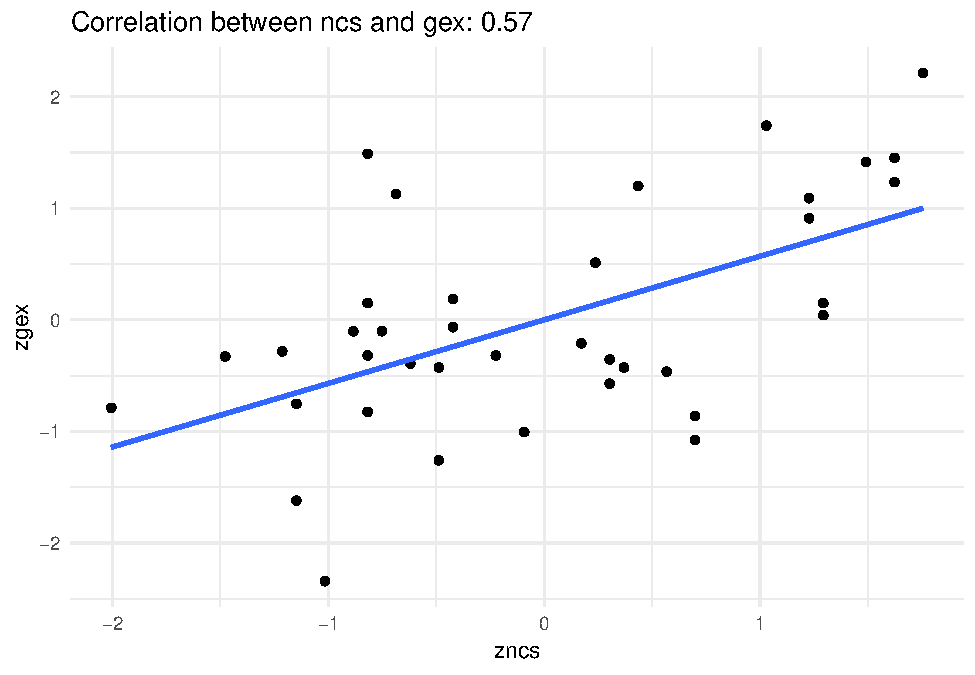
\includegraphics{Classic_linear_models_files/figure-latex/AUP_corr_predictors-1.pdf}

\begin{Shaded}
\begin{Highlighting}[]
\KeywordTok{detach}\NormalTok{(AUP)}
\end{Highlighting}
\end{Shaded}

Participants with a higher NCS also tend to have more geekism. Is that
surprising? Actually, it is not. People high on NCS love to think.
Computers are a good choice for them, because these are complicated
devices that make you think. (Many users may even agree that computers
help you think, for example when analyzing your data with R.) In turn,
geekism is a positive attitude towards working with computers in
sophisticated ways, which means such people are more resistant towards
the AUP.

{[}NCS: love to think{]} --\textgreater{} {[}GEX: love computers{]}
--\textgreater{} {[}resist AUP{]}

When such a causal chain can be established, some researchers speak of a
\emph{mediating variable} GEX. Although a bit outdated {[}REF{]},
\emph{mediator analysis is correct when the causal direction of the
three variables is known}. Then, a so-called step-wise regression is
performed to find the pure effects. (A better alternative is structural
equation modelling, SEM).

Unfortunately, in the situation here, the causal direction is partly
ambiguous. We can exclude that the resistance test has influenced the
personality scores, because of the order of apperance in the study. But,
causally speaking, geekism may well preceed NCS. For example, computers
reward you for thinking hard and, hence, you get used to it and make it
your lifestyle. If you like thinking hard, then you probably also like
the challenge that was given in the experiment.

{[}GEX: love computers{]} --\textgreater{} {[}NCS: love to think{]}
--\textgreater{} {[}resist AUP{]}

In the current case, we can not distinguish between these two competing
theories by data alone. This is a central problem in empirical research.
An example, routinely re-iterated in social science methods courses is
the observation that people who are more intelligent tend to consume
more fresh vegetables. Do carrots make us smart? Perhaps, but it is
equally plausible that eating carrots is what smart people do.

The issue is that a particular direction of causality can only be
established, when all reverse directions can be excluded. Behavioural
science reseachers know of only two ways to do so:

\begin{enumerate}
\def\labelenumi{\arabic{enumi}.}
\tightlist
\item
  By the \emph{arrow of time}, it is excluded that a later event caused
  a preceding one. In the AUP study, there is no doubt that filling out
  the two personality questionnaires cause the behaviour in the computer
  task, because of the temporal order.
\item
  In \emph{strictly controlled experiments}, participants are assigned
  to the conditions, randomly. That has (virtually) happened in the
  BrowsingAB case, which gives it an unambiguous causal direction. This
  was not so, if participants had been allowed to choose themselves
  which design to test.
\end{enumerate}

To come back to the AUP study: There is no way to establish a causal
order of predictors. The correct procedure is to regard the predictors
simultaneously (not step-wise), as in model \texttt{M\_3}. This results
in a redistribution of the overall covariance and the predictors are
\emph{mutually controlled}. In \texttt{M\_2} the effect of GEX was
promising at first, but then became spurious in the simultaneous model.
Most of the strength was just borrowed from NCS by covariation. The
model suggests that loving-to-think has a quite stronger association
with AUP resistance than loving-computers.

That \emph{may} suggest, but not prove, that geekism precedes NCS, as in
a chain of causal effects, elements that are closer to the final outcome
(AUP resistance), tend to exert more salient influence. But, without
further theorizing and experimenting this is weak evidence of causal
order.

The readers of a paper on geekism, NCS and the AUP will probably be more
impressed by the (still moderate) effects in the separate models we had
run, initially. The reason why one should not do that is that separate
analyses suggest that the predictors are independent. To illustrate this
at an extreme example, think of a study where users were asked to rate
their agreement with an interface by the following two questions, before
ToT is recorded:

\begin{enumerate}
\def\labelenumi{\arabic{enumi}.}
\tightlist
\item
  The interface is beautiful
\item
  The interface has an aesthetic appearance?
\end{enumerate}

Initial separate analysis shows strong effects for both predictors.
Still, it would not make sense to give the report the title: ``Beauty
and aesthetics predict usability''. Beauty and aesthetics are
practically synonyms. For Gex and NCS this may be not so clear, but we
cannot exclude the possibility that they are linked to a common factor,
perhaps a third trait that makes people more explorative, no matter
whether it be thoughts or computers.

So, what to do, when two predictors correlate strongly? First, we always
report just a single model. Per default, this is the model with both
predictors, simultaneously. The second possibility is to use a
disciplined method of \emph{model selection} @ref(model\_selection) and
remove this (or those) predictors that do not actually contribute to
prediction. The third possibility is, that the results with both
predictors become more interesting when including interaction effects
@ref(interaction\_effects)

\subsection{Crossover: multifactorial models
{[}TBC{]}}\label{crossover-multifactorial-models-tbc}

The only necessary precondition for statistical control is that you
recorded the influencing variable. This has happened in the BrowsingAB
study: the primary research question regarded the design difference, but
the careful researcher also recorded the gender of participants.

What happened to the likelihood function when we moved from GMM to CGM
and LRM? The effect of age was simply added to the intercept. For model
on education level effects, we expanded the dummy variables and then
added them all up. Indeed, the linear model is defined as a succession
of linear terms \(x_i\beta_i\) and nothing keeps us from adding further
predictors to the model. Seeing is believing! The following code
estimates a model with design and gender as predictors.

\begin{Shaded}
\begin{Highlighting}[]
\KeywordTok{attach}\NormalTok{(BrowsingAB)}
\end{Highlighting}
\end{Shaded}

\begin{Shaded}
\begin{Highlighting}[]
\NormalTok{M_mpm_}\DecValTok{1}\NormalTok{ <-}\StringTok{ }
\StringTok{  }\NormalTok{BAB1 }\OperatorTok\StringTok{ }
\StringTok{  }\KeywordTok{stan_glm}\NormalTok{(ToT }\OperatorTok{~}\StringTok{ }\NormalTok{Design }\OperatorTok{+}\StringTok{ }\NormalTok{Gender, }\DataTypeTok{data =}\NormalTok{ .)}
\end{Highlighting}
\end{Shaded}

\begin{Shaded}
\begin{Highlighting}[]
\NormalTok{T_fixef_mpm_}\DecValTok{1}\NormalTok{ <-}\StringTok{ }\KeywordTok{fixef}\NormalTok{(M_mpm_}\DecValTok{1}\NormalTok{)}
\NormalTok{T_fixef_mpm_}\DecValTok{1}
\end{Highlighting}
\end{Shaded}

\begin{longtable}[]{@{}lrrr@{}}
\toprule
fixef & center & lower & upper\tabularnewline
\midrule
\endhead
Intercept & 203.349 & 191.9 & 215.10\tabularnewline
DesignB & -15.050 & -27.8 & -2.68\tabularnewline
GenderM & 0.196 & -12.8 & 12.71\tabularnewline
\bottomrule
\end{longtable}

By adding gender to the model, both effects are estimated
simultaneously. In a \emph{factorial MPM} the intercept is a reference
group, too. Consider that both factors have two levels, forming a
\(2x 2\) design with groups: A-F, A-M, B-F, B-M. The first one, A-F, has
been set as reference group. Women in condition A have an average ToT of
\(203.35 [191.94, 215.1]_{CI95}\) seconds. The other two fixed effects
are, once again, differences to the reference. Here, nor does gender do
much to performance, nor does the design effect really change, compared
to the CGM.

{[}likelihood{]}{[}interaction plot{]}

\subsection{Line-by-line: regression in groups
{[}TBC{]}}\label{line-by-line}

Recall that dummy variables make factors compatible with linear
regression. No barriers are left for combining factors and covariates in
one model. For example, we can estimate the effects age and design
simultaneously:

\begin{Shaded}
\begin{Highlighting}[]
\NormalTok{M_mpm_}\DecValTok{2}\NormalTok{ <-}\StringTok{ }
\StringTok{  }\NormalTok{BAB1 }\OperatorTok\StringTok{ }
\StringTok{  }\KeywordTok{stan_glm}\NormalTok{(ToT }\OperatorTok{~}\StringTok{ }\NormalTok{Design }\OperatorTok{+}\StringTok{ }\NormalTok{age_shft, }\DataTypeTok{data =}\NormalTok{ .)}
\end{Highlighting}
\end{Shaded}

\begin{Shaded}
\begin{Highlighting}[]
\NormalTok{T_fixef_mpm_}\DecValTok{2}\NormalTok{ <-}\StringTok{  }\KeywordTok{fixef}\NormalTok{(M_mpm_}\DecValTok{2}\NormalTok{)}
\NormalTok{T_fixef_mpm_}\DecValTok{2}
\end{Highlighting}
\end{Shaded}

\begin{longtable}[]{@{}lrrr@{}}
\toprule
fixef & center & lower & upper\tabularnewline
\midrule
\endhead
Intercept & 184.208 & 169.940 & 198.79\tabularnewline
DesignB & -14.981 & -27.804 & -2.14\tabularnewline
age\_shft & 0.648 & 0.254 & 1.03\tabularnewline
\bottomrule
\end{longtable}

\begin{Shaded}
\begin{Highlighting}[]
\KeywordTok{detach}\NormalTok{(BrowsingAB)}
\end{Highlighting}
\end{Shaded}

Once again, we get an intercept, first. Recall, that in LRM the
intercept is the the performance of a 20-year old (age shifted). In GCM
it was the mean of the reference group. When \emph{marrying factors with
a covariates, the intercept is point zero in the reference group}. The
predicted average performance of 20-year old with design A is
\(184.21 [169.94, 198.79]_{CI95}\). The age effect has the usual
meaning: by year of life, participants get \(0.65 [0.25, 1.03]_{CI95}\)
seconds slower. The \emph{factorial effect} B is a \emph{vertical shift
of the intercept}. 20-year old in condition B are
\(14.98 [27.8, 2.14]_{CI95}\) seconds faster. In fact, this holds for
all ages, as can be seen in the following figure. The model implies that
the age affect is the same with both designs, which is not true, as we
will see later.

{[}likelihood{]}{[}interaction plot{]}

\subsection{Residual analysis}\label{residual-analysis}

\subsubsection{Assessing predictive power}\label{resid_predictive_power}

\begin{Shaded}
\begin{Highlighting}[]
\KeywordTok{attach}\NormalTok{(BrowsingAB)}
\end{Highlighting}
\end{Shaded}

When residuals are pronounced, predictions are inaccurate, which is
undesireable. A model that reduces the residuals, may provide better
predictions. In the current case, we may wonder: does the age predictor
effectively reduce the residual standard error \(\sigma_\epsilon\) as
compared to the GMM? We fit the GMM for comparison purposes and compare
the standard error. This does not look convincing, as the reduction is
marginal.

\begin{Shaded}
\begin{Highlighting}[]
\NormalTok{M_}\DecValTok{0}\NormalTok{ <-}
\StringTok{  }\NormalTok{BAB1 }\OperatorTok\StringTok{ }
\StringTok{  }\KeywordTok{stan_glm}\NormalTok{(ToT }\OperatorTok{~}\StringTok{ }\DecValTok{1}\NormalTok{, }\DataTypeTok{data =}\NormalTok{ .)}
\end{Highlighting}
\end{Shaded}

\begin{Shaded}
\begin{Highlighting}[]
\KeywordTok{bind_rows}\NormalTok{(}
  \KeywordTok{posterior}\NormalTok{(M_}\DecValTok{0}\NormalTok{),}
  \KeywordTok{posterior}\NormalTok{(M_age_cntr)) }\OperatorTok\StringTok{ }
\StringTok{  }\KeywordTok{coef}\NormalTok{(}\DataTypeTok{type =} \StringTok{"disp"}\NormalTok{)}
\end{Highlighting}
\end{Shaded}

\begin{longtable}[]{@{}lrrr@{}}
\toprule
model & center & lower & upper\tabularnewline
\midrule
\endhead
M\_0 & 46.1 & 42.0 & 51.2\tabularnewline
M\_age\_cntr & 45.2 & 41.1 & 49.9\tabularnewline
\bottomrule
\end{longtable}

Does the age variable really have that little predictive value? Seeing
is believing. The following graph shows the individual residuals for
both models as a column plot. The two caterpillars have about the same
overall width and there is no noticable reduction in residual magnitude
by adding the age predictor.

\begin{Shaded}
\begin{Highlighting}[]
\NormalTok{T_resid <-}
\StringTok{  }\NormalTok{BAB1 }\OperatorTok\StringTok{ }
\StringTok{  }\KeywordTok{select}\NormalTok{(Obs, age) }\OperatorTok\StringTok{ }
\StringTok{  }\KeywordTok{mutate}\NormalTok{(}
    \DataTypeTok{M_0 =} \KeywordTok{residuals}\NormalTok{(M_}\DecValTok{0}\NormalTok{),}
    \DataTypeTok{M_age =} \KeywordTok{residuals}\NormalTok{(M_age))}

\NormalTok{G_resid_age_}\DecValTok{1}\NormalTok{ <-}
\StringTok{  }\NormalTok{T_resid }\OperatorTok
\StringTok{  }\KeywordTok{mutate}\NormalTok{(}\DataTypeTok{Obs_ordered =} \KeywordTok{min_rank}\NormalTok{(age)) }\OperatorTok\StringTok{ }
\StringTok{  }\KeywordTok{gather}\NormalTok{(model, error, }\OperatorTok{-}\NormalTok{Obs, }\OperatorTok{-}\NormalTok{Obs_ordered, }\OperatorTok{-}\NormalTok{age) }\OperatorTok
\StringTok{  }\KeywordTok{ggplot}\NormalTok{(}\KeywordTok{aes}\NormalTok{(}\DataTypeTok{x =}\NormalTok{ Obs, }\DataTypeTok{y =}\NormalTok{ error)) }\OperatorTok{+}
\StringTok{  }\KeywordTok{facet_grid}\NormalTok{(}\OperatorTok{~}\NormalTok{model) }\OperatorTok{+}
\StringTok{  }\KeywordTok{geom_col}\NormalTok{(}\DataTypeTok{position =} \StringTok{"dodge"}\NormalTok{) }\OperatorTok{+}
\StringTok{  }\KeywordTok{geom_quantile}\NormalTok{()}
\NormalTok{G_resid_age_}\DecValTok{1}
\end{Highlighting}
\end{Shaded}

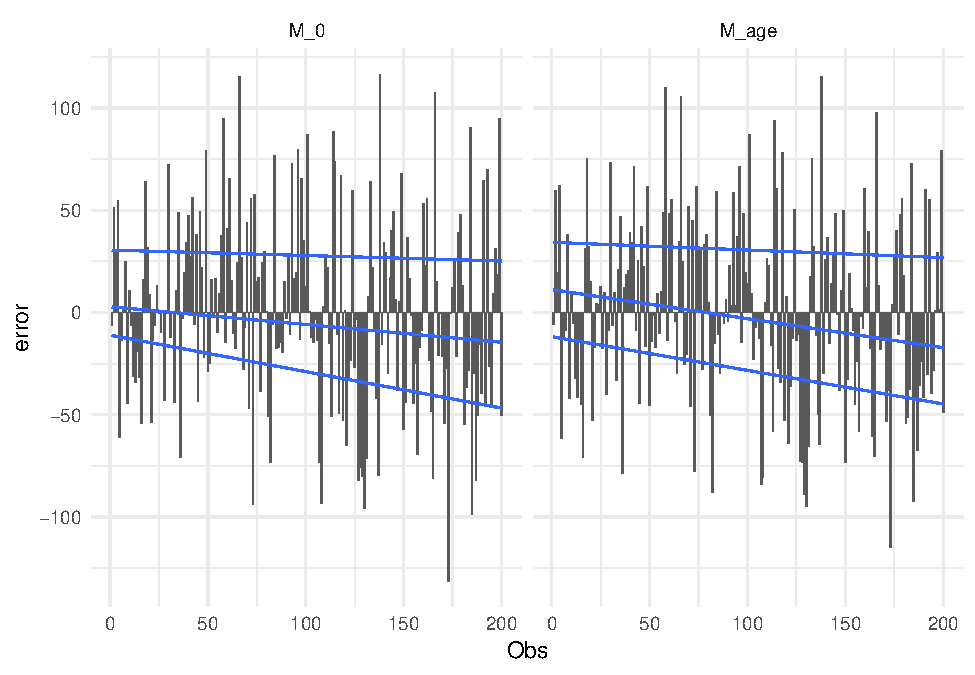
\includegraphics{Classic_linear_models_files/figure-latex/BAB1_resid_age_1-1.pdf}

When adding a predictor to a model, the least one would expect is a
noticable reduction in error and @ref(BAB1\_resid\_age\_1) confirms that
the age predictor is pretty useless.

\begin{Shaded}
\begin{Highlighting}[]
\KeywordTok{detach}\NormalTok{(BrowsingAB)}
\end{Highlighting}
\end{Shaded}

\subsubsection{Normal distribution}\label{resid_normality}

So far, we have seen two linear models, the GMM and the LRM. They only
differ in how they sketch the relation between predictor variables and
predicted values. In the remainder of this chapter on linear models, we
will encounter a few more building blocks for the likelihood part and
these will allow us to specify a wealth of complex models. However, the
random term will stoically stay the same:

\[y_i \sim N(\mu_i, \sigma_\epsilon)\]

In words, the random term says: \emph{observed values \(y_i\) are drawn
from a Normal distribution with the predicted value \(\mu_i\) as mean
and a fixed standard deviation \(\sigma_\epsilon\)}. As we have seen in
\ref{distributions}, Normal distributions are one pattern of randomness
among many and this choice may therefore be appropriate, or not. One
heuristic that may justify this choice is that the observed values are
located rather in the center of the scale of measurement. That is
certainly much better, than to blindly stick to the Normal random
pattern just for convenience. Even better is to check the assumption of
Normally distributed randomness. In the following, we will examine the
underlying assumptions closer and apply graphical techniques for
verification. Before we delve into more depth, I would like to contrast
the overall tenor in this section (and {[}MODSEL{]}) to the workflow
frequently encountered in classic statistics. Boldly speaken,
classicically trained researchers often sem to imply, that such
assumptions needed to be checked beforehand. In the process called
\emph{assumption checking}, arcane non parametric tests are carried out,
before the researcher actually dares to hit the button labelled as
\emph{RUN ANOVA}. As we will see now, the order of actions is just the
other way round. In the workflow called \emph{model criticism}, we start
by contemplating what may be a reasonable model, using heuristics or
even past data. Then the model is immediatly executed and the estimated
model itself undergoes a routine checkup. In linear models, verifying
the random pattern assumptions grounds on extracting the estimated
residuals from the model object and is hence called \emph{residual
analysis}.

In the notation displayed above, there are possibly as many
distributions as there are observed values (due the subscript in
\(\mu_i\)). It appears impossible to evaluate not just one distribution
but such many. However, an equivalent notation is routinely used for
linear models, that specifies just one \emph{residual distribution}. For
the LRM that is:

\[
\mu_i = \beta_0 + \beta_1x_1\\
y_i = \mu_i + \epsilon_i\\
\epsilon_i \sim N(0, \sigma_\epsilon)
\]

In this notation, observed values \(y_i\) are decomposed into predicted
values and \emph{individual} residuals \(\epsilon_i\). These are
frequently called \emph{errors}, hence the greek symbol \(\epsilon\).
The standard deviation of residuals \(\sigma_\epsilon\) is commonly
called the \emph{standard error}. The random pattern of the model can
now be expressed as a single Normal distribution. The reason why I do
not use this notation routinely, is that it only works for linear
models, but not for models with other random patterns. More
specifically, Generalized Linear Models
@ref(generalized\_linear\_models) cannot be specified that way. But, for
the purpose of residual analysis, it appears more intuitive.

The first assumption of randomness underlying the linear model simply is
that the distribution follows Normal distribution. Visually, Normal
distributions is characterized by:

\begin{itemize}
\tightlist
\item
  one curved peak (unimodality)
\item
  from which density smoothly declines towards both ends (smoothness)
\item
  at same rates (symmetrity)
\end{itemize}

For a rough evaluation of this assumption, it suffices to extract the
residuals from the model at hand and plot it as a distribution. The
\texttt{residuals} command returns a vector of residual values, exactly
one per observation. With the vector of residuals at hand, we can
evaluate this assumption by comparing the residual distribution to its
theoretical form, a perfect bell curve. The following command chain
extracts the residuals from the model and pipes them into the ggplot
engine to create a histogram. With \texttt{stat\_function} an overlay is
created with the theoretical Normal distribution, which is centered at
zero. The standard error \(\sigma_\epsilon\) has been estimated
alongside the coefficients and is extracted using the function
\texttt{bayr::coef}.

\begin{Shaded}
\begin{Highlighting}[]
\KeywordTok{attach}\NormalTok{(BrowsingAB)}
\end{Highlighting}
\end{Shaded}

\begin{Shaded}
\begin{Highlighting}[]
\NormalTok{G_resid_age_shft <-}
\StringTok{  }\KeywordTok{data.frame}\NormalTok{(}\DataTypeTok{resid =} \KeywordTok{residuals}\NormalTok{(M_age_shft)) }\OperatorTok\StringTok{ }
\StringTok{  }\KeywordTok{ggplot}\NormalTok{(}\KeywordTok{aes}\NormalTok{(}\DataTypeTok{x =}\NormalTok{ resid)) }\OperatorTok{+}\StringTok{ }
\StringTok{  }\KeywordTok{geom_histogram}\NormalTok{(}\KeywordTok{aes}\NormalTok{(}\DataTypeTok{y =}\NormalTok{ ..density..), }\DataTypeTok{bins =} \DecValTok{15}\NormalTok{) }\OperatorTok{+}
\StringTok{  }\KeywordTok{stat_function}\NormalTok{(}\DataTypeTok{fun =}\NormalTok{ dnorm, }
                \DataTypeTok{args =} \KeywordTok{c}\NormalTok{(}\DataTypeTok{mean =} \DecValTok{0}\NormalTok{, }
                         \DataTypeTok{sd =} \KeywordTok{coef}\NormalTok{(M_age_shft, }\DataTypeTok{type =} \StringTok{"disp"}\NormalTok{)}\OperatorTok{$}\NormalTok{center), }
                \DataTypeTok{colour =} \StringTok{"red"}\NormalTok{)}

\NormalTok{G_resid_age_shft}
\end{Highlighting}
\end{Shaded}

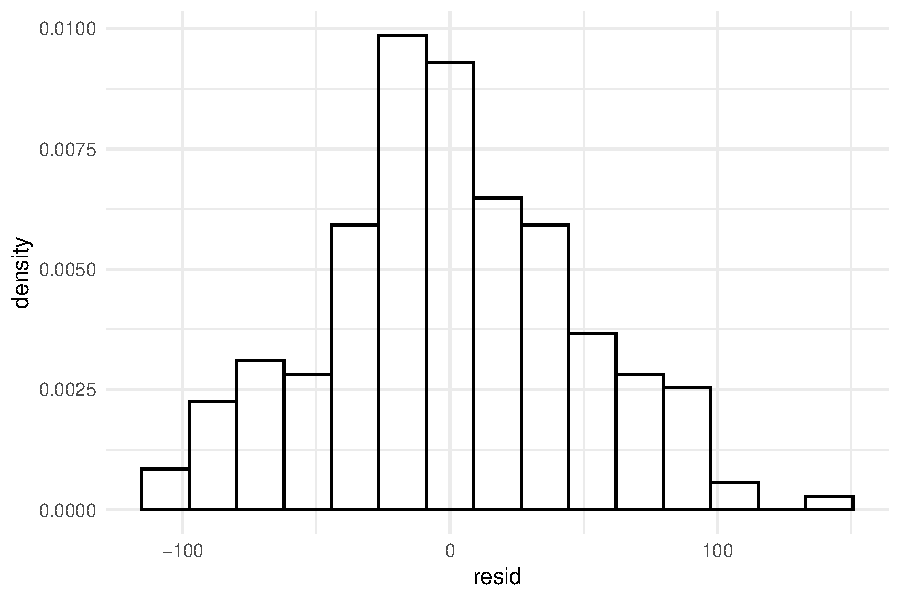
\includegraphics{Classic_linear_models_files/figure-latex/resid_dist_1-1.pdf}

The match of residual distribution with the theoretical distribution is
not perfect, but overall this model seems to sufficiently satisfy the
Normality assumption. To give a counter example, we estimate the same
model using the outcome variable \texttt{returns}, which captures the
number of times a participant had (desparately) returned to the
homepage.

\begin{Shaded}
\begin{Highlighting}[]
\NormalTok{M_age_rtrn <-}\StringTok{ }
\StringTok{  }\KeywordTok{stan_glm}\NormalTok{(returns }\OperatorTok{~}\StringTok{ }\DecValTok{1} \OperatorTok{+}\StringTok{ }\NormalTok{age_shft, }\DataTypeTok{data =}\NormalTok{ BAB1)}
\NormalTok{P_age_rtrn <-}\StringTok{ }\KeywordTok{posterior}\NormalTok{(M_age_rtrn)}
\end{Highlighting}
\end{Shaded}

\begin{Shaded}
\begin{Highlighting}[]
\NormalTok{T_age_rtrn <-}\StringTok{ }\KeywordTok{coef}\NormalTok{(P_age_rtrn)}
\NormalTok{T_age_rtrn}
\end{Highlighting}
\end{Shaded}

\begin{longtable}[]{@{}lllrrr@{}}
\toprule
parameter & type & fixef & center & lower & upper\tabularnewline
\midrule
\endhead
Intercept & fixef & Intercept & 2.563 & 1.99 & 3.099\tabularnewline
age\_shft & fixef & age\_shft & -0.004 & -0.02 & 0.013\tabularnewline
sigma\_resid & disp & NA & 1.875 & 1.71 & 2.073\tabularnewline
\bottomrule
\end{longtable}

\begin{Shaded}
\begin{Highlighting}[]
\NormalTok{C_age_rtrn_disp <-}\StringTok{ }
\StringTok{  }\NormalTok{T_age_rtrn }\OperatorTok\StringTok{ }
\StringTok{  }\KeywordTok{filter}\NormalTok{(type }\OperatorTok{==}\StringTok{ "disp"}\NormalTok{) }\OperatorTok\StringTok{ }
\StringTok{  }\KeywordTok{select}\NormalTok{(center) }\OperatorTok\StringTok{ }
\StringTok{  }\KeywordTok{as.numeric}\NormalTok{()}

\NormalTok{G_resid_age_rtrn <-}
\StringTok{  }\KeywordTok{data_frame}\NormalTok{(}\DataTypeTok{resid =} \KeywordTok{residuals}\NormalTok{(M_age_rtrn)) }\OperatorTok\StringTok{ }
\StringTok{  }\KeywordTok{ggplot}\NormalTok{(}\KeywordTok{aes}\NormalTok{(}\DataTypeTok{x =}\NormalTok{ resid)) }\OperatorTok{+}\StringTok{ }
\StringTok{  }\KeywordTok{geom_histogram}\NormalTok{(}\KeywordTok{aes}\NormalTok{(}\DataTypeTok{y =}\NormalTok{ ..density..), }\DataTypeTok{bins =} \DecValTok{10}\NormalTok{) }\OperatorTok{+}
\StringTok{  }\KeywordTok{stat_function}\NormalTok{(}\DataTypeTok{fun =}\NormalTok{ dnorm, }
                \DataTypeTok{args =} \KeywordTok{c}\NormalTok{(}\DataTypeTok{mean =} \DecValTok{0}\NormalTok{, }
                         \DataTypeTok{sd =}\NormalTok{ C_age_rtrn_disp), }
                \DataTypeTok{colour =} \StringTok{"red"}\NormalTok{) }\OperatorTok{+}
\StringTok{  }\KeywordTok{xlim}\NormalTok{(}\OperatorTok{-}\DecValTok{5}\NormalTok{, }\DecValTok{5}\NormalTok{)}
\NormalTok{G_resid_age_rtrn}
\end{Highlighting}
\end{Shaded}

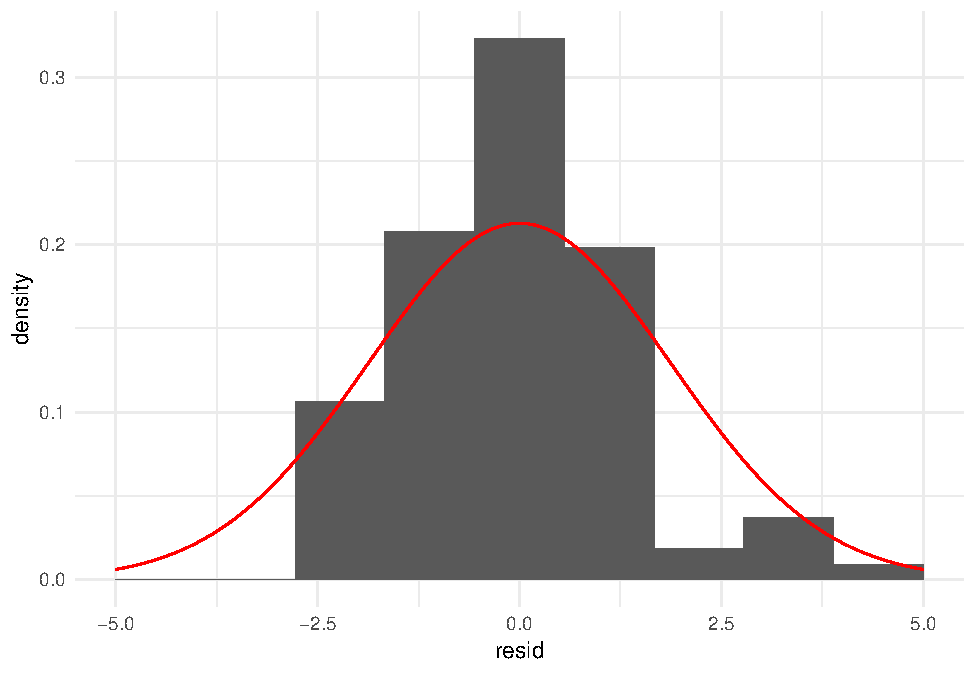
\includegraphics{Classic_linear_models_files/figure-latex/resid_dist_2-1.pdf}

\begin{Shaded}
\begin{Highlighting}[]
\KeywordTok{detach}\NormalTok{(BrowsingAB)}
\end{Highlighting}
\end{Shaded}

The estimation produces the usual coefficients, as well as a standard
error. However, the residuals not even remotely resemble the theoretical
curve. While it is unimodal, it appears rather asymmetric, with a steep
rise to the left and a long tail to the right. That is a typical outcome
when count measures get too close to the left boundary. How about
unimodality? We have not discussed any multimodal theoretical
distributions in \ref{distributions}, but one has been displayed in
@ref(first\_program). In brief, a bimodal residual distribution can
arise, when two groups exist in the data, which lay far apart. The
following code illustrates the situation by simulating a simple data set
with two groups, that is fed into a GMM.

\begin{Shaded}
\begin{Highlighting}[]
\KeywordTok{attach}\NormalTok{(Chapter_LM)}
\end{Highlighting}
\end{Shaded}

\begin{Shaded}
\begin{Highlighting}[]
\KeywordTok{set.seed}\NormalTok{(}\DecValTok{42}\NormalTok{)}
\NormalTok{D_bimod <-}\StringTok{ }
\StringTok{  }\KeywordTok{bind_rows}\NormalTok{(}
    \KeywordTok{data_frame}\NormalTok{(}\DataTypeTok{Group =} \StringTok{"A"}\NormalTok{, }\DataTypeTok{y =} \KeywordTok{rnorm}\NormalTok{(}\DecValTok{50}\NormalTok{, }\DecValTok{4}\NormalTok{, }\DecValTok{1}\NormalTok{)),}
    \KeywordTok{data_frame}\NormalTok{(}\DataTypeTok{Group =} \StringTok{"B"}\NormalTok{, }\DataTypeTok{y =} \KeywordTok{rnorm}\NormalTok{(}\DecValTok{50}\NormalTok{, }\DecValTok{8}\NormalTok{, }\DecValTok{1}\NormalTok{))}
\NormalTok{  )}
\end{Highlighting}
\end{Shaded}

\begin{Shaded}
\begin{Highlighting}[]
\NormalTok{M_bimod <-}\StringTok{ }\KeywordTok{stan_glm}\NormalTok{(y }\OperatorTok{~}\StringTok{ }\DecValTok{1}\NormalTok{, }\DataTypeTok{data =}\NormalTok{ D_bimod, }\DataTypeTok{iter =} \DecValTok{200}\NormalTok{)}
\end{Highlighting}
\end{Shaded}

\begin{Shaded}
\begin{Highlighting}[]
\NormalTok{D_bimod  }\OperatorTok\StringTok{  }
\StringTok{  }\KeywordTok{mutate}\NormalTok{(}\DataTypeTok{resid =} \KeywordTok{residuals}\NormalTok{(M_}\DecValTok{1}\NormalTok{)) }\OperatorTok\StringTok{ }
\StringTok{  }\KeywordTok{ggplot}\NormalTok{(}\KeywordTok{aes}\NormalTok{(}\DataTypeTok{x =}\NormalTok{ resid)) }\OperatorTok{+}
\StringTok{  }\KeywordTok{geom_density}\NormalTok{()}
\end{Highlighting}
\end{Shaded}

\includegraphics{Classic_linear_models_files/figure-latex/unnamed-chunk-55-1.pdf}

These two deviations from Normal distribution have very different
causes: asymmetry is caused by scales with boundaries. This is an often
arising situation and it is gracefully solved by Generalized Linear
Models \ref{GLM}. This is a family of models, where each member covers a
certain type of measurement scale. In the above example, Poisson
regression, applies, taking care of count measures. Mulitmodality is
caused by heterogeneous groups in the data, like experimental
conditions, design or type of user. For a grouping structure to cause
distinguished multimodality, differences between groups have to be
pronounced, in relation to the standard error. It is often the case,
that these variables are controlled conditions, such as in an AB test.
It is also quite likely that strong grouping structures can be thought
of beforehand and be recorded. For example, in usability tests with
diverse user samples, in almost comes natural to distinguiish between
users who have used the design before, and those who didn't. If the
grouping variable is recorded, the solution is group comparison models
\ref{CGM}, soon to be introduced.

Visual assessment of symmetry and unimodality is simple and effective in
many cases. But, Normal distributions are not the only to have these
properties. At least logistic distributions and t distributions have
these, too, with subtle different in curvature. Normal and t
distributions differ in how quickly probability drops in the tails.
Normal distributions drop much faster such that extreme events are
practically impossible. With t-distributions, extreme values drop in
probability, too, but the possibility of catastrophies (or wonders)
stays substantial for a long time.

Provided one has a small abundance of data, \emph{quantile-quantile (qq)
plots} can be used to evaluate subtle deviations in curvature (and
symmetry and unimodality). In qq plots, the observed and theoretical
distributions are both flattened and put against each other. This is a
powerful and concise method, but it is harder to grasp. The following
code illustrates the construction of a qq-plot that compares GMM
residuals of a t-distributed measure against the Normal distribution. We
simulate t-distributed data, run a GMM and extract residuals, as well as
the standard error \(\sigma_\epsilon\).

\begin{Shaded}
\begin{Highlighting}[]
\KeywordTok{set.seed}\NormalTok{(}\DecValTok{2}\NormalTok{)}
\NormalTok{D_t <-}\StringTok{ }\KeywordTok{data_frame}\NormalTok{(}\DataTypeTok{y =} \KeywordTok{rt}\NormalTok{(}\DecValTok{200}\NormalTok{, }\DecValTok{2}\NormalTok{))}
\end{Highlighting}
\end{Shaded}

\begin{Shaded}
\begin{Highlighting}[]
\NormalTok{M_t <-}\StringTok{ }\KeywordTok{stan_glm}\NormalTok{(y }\OperatorTok{~}\DecValTok{1}\NormalTok{, }\DataTypeTok{data =}\NormalTok{ D_t, }\DataTypeTok{iter =} \DecValTok{200}\NormalTok{)}
\end{Highlighting}
\end{Shaded}

We obtain the following residual and theoretical distributions. It is
approximately symmetric and unimodal, but the curvature seems to be a
bit off.

\begin{Shaded}
\begin{Highlighting}[]
\NormalTok{D_t <-}\StringTok{   }\KeywordTok{mutate}\NormalTok{(D_t, }\DataTypeTok{resid =} \KeywordTok{residuals}\NormalTok{(M_t))}

\NormalTok{C_sigma <-}\StringTok{ }\NormalTok{rstanarm}\OperatorTok{::}\KeywordTok{sigma}\NormalTok{(M_t)}

\NormalTok{D_t }\OperatorTok
\StringTok{  }\KeywordTok{ggplot}\NormalTok{(}\KeywordTok{aes}\NormalTok{(}\DataTypeTok{x =}\NormalTok{ resid)) }\OperatorTok{+}
\StringTok{  }\KeywordTok{geom_histogram}\NormalTok{(}\KeywordTok{aes}\NormalTok{(}\DataTypeTok{y =}\NormalTok{ ..density..)) }\OperatorTok{+}
\StringTok{  }\KeywordTok{stat_function}\NormalTok{(}\DataTypeTok{fun =}\NormalTok{ dnorm,}
                \DataTypeTok{args =} \KeywordTok{c}\NormalTok{(}\DataTypeTok{mean =} \DecValTok{0}\NormalTok{,}
                         \DataTypeTok{sd =}\NormalTok{ C_sigma),}
                \DataTypeTok{colour =} \StringTok{"red"}\NormalTok{)}
\end{Highlighting}
\end{Shaded}

\includegraphics{Classic_linear_models_files/figure-latex/unnamed-chunk-58-1.pdf}

The next step is where the two curves get flattened. First, we compute a
sequence of quantiles with fixed steps, say 1\%, 2\%, \ldots{} 99\%\%.
Finally, theoretical and observed quantiles are fed into a scatterplot.

\begin{Shaded}
\begin{Highlighting}[]
\NormalTok{D_QQ <-}\StringTok{ }\KeywordTok{data_frame}\NormalTok{(}\DataTypeTok{step =} \DecValTok{0}\OperatorTok{:}\DecValTok{100}\OperatorTok{/}\DecValTok{100}\NormalTok{,}
           \DataTypeTok{quant_smpl =} \KeywordTok{quantile}\NormalTok{(D_t}\OperatorTok{$}\NormalTok{resid, step),}
           \DataTypeTok{quant_theo =} \KeywordTok{qnorm}\NormalTok{(step, }\DecValTok{0}\NormalTok{, C_sigma))}

\NormalTok{D_QQ }\OperatorTok\StringTok{ }
\StringTok{  }\KeywordTok{ggplot}\NormalTok{(}\KeywordTok{aes}\NormalTok{(}\DataTypeTok{x =}\NormalTok{ quant_theo, }\DataTypeTok{y =}\NormalTok{ quant_smpl)) }\OperatorTok{+}
\StringTok{  }\KeywordTok{geom_point}\NormalTok{() }\OperatorTok{+}
\StringTok{  }\KeywordTok{geom_abline}\NormalTok{(}\DataTypeTok{slope =} \DecValTok{1}\NormalTok{, }\DataTypeTok{intercept =} \DecValTok{0}\NormalTok{, }\DataTypeTok{col =} \StringTok{"red"}\NormalTok{)}
\end{Highlighting}
\end{Shaded}

\includegraphics{Classic_linear_models_files/figure-latex/unnamed-chunk-59-1.pdf}

In the ideal case, they match perfectly, and the quantiles are on a
straight line. Instead, we see a rotated sigmoid shape and this is
typical for fat-tailed distributions such as t. The shape is symmetric
with turning points at around -4 and 4 on the theoretical scale. In the
middle part the relation is almost linear, however, not matching a
1-by-1. The t distribution loses probability mass rather quickly when
moving from the center to the tuzrning points. here. From these points
on the theoretical quantiles start lag behind. The lower and upper 1\%
sampled quantiles go to much more extreme values, ranging from -10 to
almost 20, whereas the Normal distribution renders such events
practically impossible. Generally, a rotated sigmoid shape is typical
for fat tailed distributions. The problem of misusing a Normal
distribution is that it dramatically underestimates extreme events. Have
you ever asked yourself, why in the 1990s, the risk for a nuclear
meltdown were estimated to be one in 10.000 years, in face of two such
tragic events in the past 40 years? Perhaps, researchers used the Normal
distribution for the risk models, under-estimating the risk of extreme
events.

The ggplot engine provides an easy to use geometry for qqlots, which
lets us further explore deviant patterns. Variables with t distribution
take an inverse-sigmoid shape due to their fat tails.

\begin{Shaded}
\begin{Highlighting}[]
\NormalTok{D_t }\OperatorTok\StringTok{ }
\StringTok{  }\KeywordTok{ggplot}\NormalTok{(}\KeywordTok{aes}\NormalTok{(}\DataTypeTok{sample =}\NormalTok{ resid)) }\OperatorTok{+}
\StringTok{  }\KeywordTok{geom_qq}\NormalTok{(}\DataTypeTok{distribution =}\NormalTok{ qnorm) }\OperatorTok{+}
\StringTok{  }\KeywordTok{geom_abline}\NormalTok{(}\DataTypeTok{intercept =} \DecValTok{0}\NormalTok{, }\DataTypeTok{slope =} \DecValTok{1}\NormalTok{, }\DataTypeTok{col =} \StringTok{"red"}\NormalTok{)}
\end{Highlighting}
\end{Shaded}

\includegraphics{Classic_linear_models_files/figure-latex/unnamed-chunk-61-1.pdf}

\begin{Shaded}
\begin{Highlighting}[]
\KeywordTok{detach}\NormalTok{(Chapter_LM)}
\end{Highlighting}
\end{Shaded}

Once mastered, the qq-plot is the swiss knife of Normality check. Next
to the subtleties We can also easily discover deviations from symmetry.
This is how the residuals of the returns to homepage model look like:

\begin{Shaded}
\begin{Highlighting}[]
  \KeywordTok{data_frame}\NormalTok{(}\DataTypeTok{resid =} \KeywordTok{residuals}\NormalTok{(BrowsingAB}\OperatorTok{$}\NormalTok{M_age_rtrn)) }\OperatorTok\StringTok{ }
\StringTok{  }\KeywordTok{ggplot}\NormalTok{(}\KeywordTok{aes}\NormalTok{(}\DataTypeTok{sample =}\NormalTok{ resid)) }\OperatorTok{+}
\StringTok{  }\KeywordTok{geom_qq}\NormalTok{(}\DataTypeTok{distribution =}\NormalTok{ qnorm) }\OperatorTok{+}
\StringTok{  }\KeywordTok{geom_abline}\NormalTok{(}\DataTypeTok{intercept =} \DecValTok{0}\NormalTok{, }\DataTypeTok{slope =} \DecValTok{1}\NormalTok{, }\DataTypeTok{col =} \StringTok{"red"}\NormalTok{)}
\end{Highlighting}
\end{Shaded}

\includegraphics{Classic_linear_models_files/figure-latex/unnamed-chunk-63-1.pdf}

To the left, extreme values have a lower probability than predicted by
the Normal distribution, but the right tail are much fatter, one again.
We also see how residuals are clumped, which is characteristic for
discrete (as compared to continuous) outcome measures. This is poor
behaviour of the model and, generally, when a model is severely
mis-spedified, neither predictions nor estimate, nor certainty
statements can be fully trusted. A model that frequently fits in case of
count numbers is Poisson regression, which will enter the stage in
chapter @ref(poisson\_regression).

\subsubsection{Constant variance}\label{resid_constant_variance}

In @ref(resid\_normality) we have assessed one assumption that underlies
all linear models, namely Normal distribution of residuals. The second
assumption underlying the linear model random (or residual) is that
residual variance is constant throughout the whole range. In both,
classic and modern notation this grounds in the there being just a
single \(\sigma_\epsilon\) defined. However large \(\mu_i\) is, the
dispersion of residuals is not supposed to change.

Before we dive into the matter of checking the assumption let's do a
brief reality check using common sense:

\begin{enumerate}
\def\labelenumi{\arabic{enumi}.}
\item
  Consider people's daily way to work. Suppose you ask a few persons you
  know: ``What is your typical way to work and what is the longest and
  the shortest duration you remember?''. In statistical terms, you are
  asking for a center estimate and (informal) error dispersion. Is it
  plausible that a person with typical travel time of 5 minutes
  experienced the same variation as another person witha typical time of
  50 minutes?
\item
  Consider an experiment to assess a typing training. Is it plausible
  that the dispersion of typing errors before the training is the same
  as after the training?
\end{enumerate}

In both cases, we would rather not expect constant variance and it is
actually quite difficult to think of a process, where a strong change in
average performance is not associated with a change in dispersion. The
constant variance assumption, like the normality assumption is a usual
suspect when approximating with linear models. We will come back to that
down below.

In a similar way, we can ask: can it be taken as granted that residual
variance is constant when comparing two or more groups. Would you
blindly assume that two rather different designs produce the same amount
spread around the average? It may be so, but one can easily think of
reasons, why this might be different. We check the situation in the CGM
of the BrowsingAB study. Do both design conditions have the same
residual variance? Again, we extract the residuals, add them to the data
set and produce a boxplot by Design condition:

\begin{Shaded}
\begin{Highlighting}[]
\KeywordTok{attach}\NormalTok{(BrowsingAB)}
\end{Highlighting}
\end{Shaded}

\begin{Shaded}
\begin{Highlighting}[]
\NormalTok{BAB1 }\OperatorTok\StringTok{ }
\StringTok{  }\KeywordTok{mutate}\NormalTok{(}\DataTypeTok{resid_Design =} \KeywordTok{residuals}\NormalTok{(M_Design)) }\OperatorTok\StringTok{ }
\StringTok{  }\KeywordTok{ggplot}\NormalTok{(}\KeywordTok{aes}\NormalTok{(}\DataTypeTok{x =}\NormalTok{ Design, }\DataTypeTok{y =}\NormalTok{ resid_Design)) }\OperatorTok{+}
\StringTok{  }\KeywordTok{geom_boxplot}\NormalTok{()}
\end{Highlighting}
\end{Shaded}

\includegraphics{Classic_linear_models_files/figure-latex/unnamed-chunk-65-1.pdf}

Both sets of residuals are reasonably symmetric, but it appears that
design B produces more widely spread residual. Something in the design
causes individual performance to vary stronger from the population mean.
The cause of this effect will be disclosed in
@ref(differential\_design\_effects). (In essence, design B is rather
efficient to use for younger users, whereas older users seem to have
severe issues.)

Visual checks of constant variance for factors is straight forward using
common boxplots. For continuous predictors, such as age, requires a more
uncommon graphical representation known as \emph{quantile plots}. These
are not the same as qq plots, but luckily are included with ggplot.

\begin{Shaded}
\begin{Highlighting}[]
\NormalTok{BAB1 }\OperatorTok\StringTok{ }
\StringTok{  }\KeywordTok{mutate}\NormalTok{(}\DataTypeTok{resid_age =} \KeywordTok{residuals}\NormalTok{(M_age)) }\OperatorTok
\StringTok{  }\KeywordTok{ggplot}\NormalTok{(}\KeywordTok{aes}\NormalTok{(}\DataTypeTok{x =}\NormalTok{ age, }\DataTypeTok{y =}\NormalTok{ resid_age)) }\OperatorTok{+}
\StringTok{  }\KeywordTok{geom_point}\NormalTok{() }\OperatorTok{+}
\StringTok{  }\KeywordTok{geom_quantile}\NormalTok{()}
\end{Highlighting}
\end{Shaded}

\includegraphics{Classic_linear_models_files/figure-latex/unnamed-chunk-66-1.pdf}

The quantile plot uses a smoothing algorithm (probably not unlike LOESS)
to picture the trend of quantiles (25\%, 50\% and 75\%). Here, the
quantiles run almost horizontal and parallel, which confirms constant
variance. Taking this as a starting point, we can evaluate more complex
models, too. The MPM on age and design, just requires to create a
grouped quantile plot. This looks best using facetting, rather than
separating by color:

\begin{Shaded}
\begin{Highlighting}[]
\NormalTok{BAB1 }\OperatorTok\StringTok{ }
\StringTok{  }\KeywordTok{mutate}\NormalTok{(}\DataTypeTok{resid_mpm_2 =} \KeywordTok{residuals}\NormalTok{(M_mpm_}\DecValTok{2}\NormalTok{)) }\OperatorTok
\StringTok{  }\KeywordTok{ggplot}\NormalTok{(}\KeywordTok{aes}\NormalTok{(}\DataTypeTok{x =}\NormalTok{ age_shft, }\DataTypeTok{y =}\NormalTok{ resid_mpm_}\DecValTok{2}\NormalTok{)) }\OperatorTok{+}
\StringTok{  }\KeywordTok{facet_grid}\NormalTok{(}\OperatorTok{~}\NormalTok{Design) }\OperatorTok{+}
\StringTok{  }\KeywordTok{geom_point}\NormalTok{() }\OperatorTok{+}
\StringTok{  }\KeywordTok{geom_quantile}\NormalTok{()}
\end{Highlighting}
\end{Shaded}

\includegraphics{Classic_linear_models_files/figure-latex/unnamed-chunk-67-1.pdf}

This looks rather worrying. Especially with Design A, the residuals are
not constant, but increase with age. In addition, we observe that
residuals are not even centered at zero across the whole range. For
design A, the residual distribution moves from positive centered to
negative centered, design B vice versa. That also casts doubts on the
validity of the LRM on age: these contrariwise trends seem to mix into
an unsuspicious even distribution. It seems that a lot more has been
going on in this study, than would be captured by any of these models.

\begin{Shaded}
\begin{Highlighting}[]
\KeywordTok{detach}\NormalTok{(BrowsingAB)}
\end{Highlighting}
\end{Shaded}

Another model type we may want to check with quantile plots is the MRM.
With two continuous predictors one might be tempted to think of a
3-dimnensional quantile plot, but this is not recommended. Rather, we
can use a generalization of quantile plots, where the x-axis is not
mapped to the predictor, directly, but the predicted values \(\mu_i\).
We assess the residual variance on the MRM model on the AUP study, where
resistance to fall for the active user paradox has been predicted by
geekism tendencies (gex) and need-for-cognition (ncs):

\begin{Shaded}
\begin{Highlighting}[]
\KeywordTok{attach}\NormalTok{(AUP)}
\end{Highlighting}
\end{Shaded}

\begin{Shaded}
\begin{Highlighting}[]
\NormalTok{AUP_}\DecValTok{1} \OperatorTok\StringTok{ }
\StringTok{  }\KeywordTok{mutate}\NormalTok{(}\DataTypeTok{resid_3 =} \KeywordTok{residuals}\NormalTok{(M_}\DecValTok{3}\NormalTok{),}
         \DataTypeTok{mu_3 =} \KeywordTok{predict}\NormalTok{(M_}\DecValTok{3}\NormalTok{)}\OperatorTok{$}\NormalTok{center) }\OperatorTok
\StringTok{  }\KeywordTok{ggplot}\NormalTok{(}\KeywordTok{aes}\NormalTok{(}\DataTypeTok{x =}\NormalTok{ mu_}\DecValTok{3}\NormalTok{, }\DataTypeTok{y =}\NormalTok{ resid_}\DecValTok{3}\NormalTok{)) }\OperatorTok{+}
\StringTok{  }\KeywordTok{geom_point}\NormalTok{() }\OperatorTok{+}
\StringTok{  }\KeywordTok{geom_quantile}\NormalTok{()}
\end{Highlighting}
\end{Shaded}

\includegraphics{Classic_linear_models_files/figure-latex/unnamed-chunk-70-1.pdf}

We observe a clear trend in quantiles, with residual dispersion
increasing with predicted values. Generally, plotting residuals against
predicted values can be done with any model, irrespectively of the
number and types of predictors. However, interpretation is more limited
than when plotting them against predictors directly. In fact,
interpretation boils down to the intuition we introduced at the
beginning of the section, that larger outcomes typically have larger
dispersion. This is almost always a compelling assumption, or even a
matter of underlying physics and, once again, a linear model may or may
not be a reasonable approximation. Fortunately, when we turn towards
@ref(generalized\_linear\_models), we will find that these models take
provide more reasonable defaults for the relationship between predicted
values and dispersion. In contrast, residual variance per predictor
allows to discover more surprising issues, such as interaction effects
or heterogeneity in groups.

\begin{Shaded}
\begin{Highlighting}[]
\KeywordTok{detach}\NormalTok{(AUP)}
\end{Highlighting}
\end{Shaded}

\subsection{How to plot MPM? {[}TBC, move to Interaction
effects{]}}\label{how-to-plot-mpm-tbc-move-to-interaction-effects}

Now that we have seen how we can compare on one factor, we can extend
the CGM to more factors. With linear models, we can extend the basic CGM
to incorporate multiple of such factors. This is called
\emph{multifactorial models} (MFM).

Now, we are looking at a slightly more complicated situation, where
browsing is predicted by design and education level of participants at
the same time.

First, with the \emph{ggplot} system, we plot the new situation. Recall
that

\begin{enumerate}
\def\labelenumi{\arabic{enumi}.}
\item
  mapping variables in the data set to elemental properties in the plot,
  such as: x position, y position, color, shape etc.
\item
  selecting an appropriate geometry that carries such properties,
  e.g.~points, bars, box plots
\end{enumerate}

Now we can do the two-factorial ANOVA in much the same way as before. We
only have to add the predictor \emph{Education} to the model formula.
Then we run the MCMC estimation and get the estimates.

{[}Interaction plots with groups, IA plots with standard debs, mixed IA
plots, using the AMM{]}

\subsection{Empirical versus statistical
control}\label{empirical-versus-statistical-control}

Fundamental researchers have a knack for the experimental method. An
\emph{experiment}, strictly, is a study where you measure the effects of
variables you \emph{manipulate}. Manipulation is, almost literally, that
it is \emph{in your hands}, who receives the treatment. The fantastic
thing about manipulation is that it allows for \emph{causal
conclusions}. A \emph{strictly controlled experiment} is when all
influencing variables are either manipulated or kept constant. That is
an ideal and would not even be the case if you test the same person
over-and-over again (like researchers in psychophysics often do). You
never jump into the same river twice.

Sometimes an influencing variables lends itself to be kept constant. For
example in cognitive psychology experiments, environment and equipment
is usually kept constant. For applied research, keeping things constant
comes at a major disadvantage: it limits the possible conclusions drawn
from the study. Imagine, you tested a smartphone app with participants,
all students, comfortably sitting in a quiet environment. Would you dare
to make conclusions on how any users perform in real life situations,
say while driving a car? When keeping things constant, \emph{ecological
validity} and \emph{generalizability} suffer.

In most applied design studies we need ecological validity and
generalizability. If performance differs under certain conditions, you
certainly want to know that. The solution is to \emph{let conditions
vary and record them} as variables, as good as possible. For example, if
you were to compare two voice-controlled intelligent agent apps, you
could manipulate the ambient noise level, if you are in the lab.

In practically all applied studies, there exist variables, which you
cannot manipulate for one of the following reasons. Especially, user
traits are impossible to manipulate. If someone has an extrovert
character or did a lot of gaming in the past, you cannot change that.
Diversity of users is a fact and people come as they are.

Field studies usually aim for high ecological validity. Participants are
supposed to use the system in the situations they encounter. If a
smartphone app is being used sitting walking, driving or on a secret
place, it is crucial to observe all situations. Consider a car
navigation system that is tested in a long, lonely highway situation.
How much would the results tell your for performance in dense city
traffic? Design researchers frequently need results that are highly
representative for users and situations of use.

Fundamental lab researchers are afraid of individual differences, too.
The reasons are different, though: all non-manipulated influencing
factors add noise to the study, which makes it harder to find the
effects of interest. While lab researchers do there best to keep the
environment constant, they cannot keep all participant traits constant.
Lab researchers have two solutions to the problem: matching and
randomized control.

With \emph{pair matching}, potentially relevant participant traits are
recorded upfront; then participants are assigned to conditions such that
groups have about the same composition. For example, one makes sure that
the age distribution is about the same and both genders are equally
represented. When all other influencing variables are constant between
groups, the lab researcher can be sure that the effect is unambiguously
caused by the manipulation. So they say and routinely record
participants age, gender and nationality.

However, there are better alternatives: the best pair match is the
person herself. Experimental studies that expose the same person to
several conditions are called \emph{within-subject}. In the special case
that all participants encounter all conditions, the variable is
\emph{complete within-subject}. {[}A special case of within-subject
design is \emph{repeated measures}.{]} In the following chapter, we use
mixed-effects models {[}LMM{]} to deal with within-subject designs,
gracefully.

In design research, pair matching applies for situations, where designs
are compared. In the simpler situation that a design is evaluated
against set standard (e.g.~111 seconds to rent a car), it is more
important to do \emph{population matching}. The sample of participants
is drawn to be \emph{representative for the target population}.
Representativeness comes in two levels: \emph{coverage representation}
is reached when all influencing properties have occurred a few times
during observation. So, if your target population contains several
subgroups, such as age groups, experience or people with different
goals, they should all be covered to some extent. \emph{Proportional
representation} means all user and situational properties are covered
\emph{and} they have about the same proportion in teh sample as in the
population.

You can only match what you can measure and you only measure what you
expect. Human behavior in everyday life is influenced by many factors in
complex ways. Although a plethora of personality inventories exists,
doing them all prior to the real study is impossible. It would probably
not even be effective. Never have i seen a design research study, where
even the most established personality tests explain more than a few
percent of variation. As another example, take the primacy effect: what
you experienced first, has the strongest influence. In real life,
impressions are constantly pouring on people and you will never be able
to record and match that to a reasonable extent.

When influencing variables cannot be measured for matching or
statistical control, the last resort is \emph{randomized control}. This
is a misleading term, insofar as what the researcher actually does is to
\emph{let go to chance}. Indeed, if the process of drawing participants
and assigning them to manipulations is completely left to chance, then
\emph{in the long-term}, the sample will be proportional representative
and all groups will have the same composition of traits.
\emph{Randomization} works well with larger samples. With small sample,
it can still easily happen that one ends up with more or less biased
samples or heterogeneous groups. Just by chance, more higher-educated
people could have ended up in condition A of BrowsingAB.

Using manipulation, matching or randomization in in-the-wild research
may work in some cases. In other cases it will be ineffective or
impractical. The ultimate problem is the attempt to keep things
constant. In applied design research the questions rarely come down to a
``Is A better than B?''. If there is an age effect, you may certainly
want to know it and see how the design effect compares to it. But, you
can only examine what is varied and recorded. The approach of
\emph{statistical control} is to record (instead of manipulate) all
variables that may influence the results and add them to the statistical
model. As we will see now, the linear model puts no limits on the number
of predictors. If you believe that user age may play a role for
performance, just record it and add it to the model. Statistical control
requires at least coverage representation of the sample.

\subsection{Exercises}\label{exercises-4}

\begin{enumerate}
\def\labelenumi{\arabic{enumi}.}
\item
  Rerun \texttt{M\_3}, this time using the unstandardized resistance
  scores. Interpret the intercept.
\item
  The innovators behind the WWW have a long tradition in figurative use
  of nautical metaphors, like navigator, cybernaut, \ldots{} Do people
  in a world-wide hypermedia system behave like animals roaming known
  and lesser known territory? Then we would expect performance to be
  dependent on abilities for spatial cognition, like the visual-spatial
  working memory. Another theory could draw on the fact that for most
  websites the written word prevails. Would we not expect people with
  better verbal processing capabilities to excel? Consider a study
  \texttt{MMN} (for Miller's magic number, an iconic term in working
  memory research) that examines the influence of working memory
  capacities on people's browsing performance. Two tests for WM capacity
  were used: the Corsi task for visual-spatial WM capacity and the Ospan
  task for verbal WM capacity. Then participants were given five
  different search tasks on five websites. As a measure of efficiency,
  total time on task and number of clicks were recorded. As these
  variables tend to have skewed residual distributions, logarithmic
  transformation was applied before analysis. \emph{Do LRM on both WM
  predictors separately, then move on to an MRM.}.
\end{enumerate}

\section{Interaction effects}\label{interaction-effects}

With the framework of MPM, we can use an arbitrary number of predictors.
These can represent properties on different levels, for example, two
designs proposals for a website can differ in font size, or participants
differ in age. So, with MPM we gain much greater flexibility in handling
data from applied design research, which allows us to examine
user-design interactions (literally) more closely.

The catch is that if you would ask an arbitrary design researcher:

\begin{quote}
Do you think that all users are equal? Or, could it be that one design
is better for some users, but inferior for others?
\end{quote}

you would in most cases get the answer:

\begin{quote}
Of course users differ in many ways and it is crucial to know your
target group.
\end{quote}

Some will also refer to the concept of usability by the ISO 9241-11,
which contains the famous four words:

\begin{quote}
``\ldots{} for a specified user \ldots{}''
\end{quote}

The definition explicitly requires you to state for \emph{for whom} you
intended to design. It thereby implicitly acknowledges that usability of
a design could be very different for another user group. In other words,
statements on usability are by the ISO 9241-11 definition
\emph{conditional} on the target user group.

In statistical terms, conditional statements of the form:

\begin{quote}
the effect of design changes with (some) user properties
\end{quote}

In regression models, conditional statements like these are represented
by \emph{interaction effects}. Interactions between user properties and
designs are the most genuine in design research, and deserve a
neologism: \emph{differential design effects (DDM)}. They come with some
of their siblings. \emph{Saturation} occurs when physical (or other)
boundaries are reached and the result is less than the sum.
\emph{Amplification}, a rare one, is like compound glue: it will harden
only if the two components are present. The final section is a plea for
interaction effects in theorizing.

\subsection{Users differ: differential design
effects}\label{differential_design_effects}

Do people differ? Yes. If you showed two web designs to a group of
stakeholders, asking to choose individually. Is there any chance they
would all agree? No. Is the design of universal systems easy? No. The
ideal of universal design is to never put a user group at a
disadvantage. If it is an ideal, than designs are likely to differ in by
how much they accomplish it.

As to age: it is commonly held that older people tend to have lower
performance than younger users. A number of factors are called
responsible, such as: slower processing speed, lower working memory
capacity, lower motor speed and visual problems. Is, perhaps, one of the
two designs less of a burden for elderly users? We plot the observed ToT
by age, this time forming groups by design.

\begin{Shaded}
\begin{Highlighting}[]
\KeywordTok{attach}\NormalTok{(BrowsingAB)}

\NormalTok{G_slope_ia <-}
\StringTok{  }\NormalTok{BAB1 }\OperatorTok
\StringTok{  }\KeywordTok{ggplot}\NormalTok{(}\KeywordTok{aes}\NormalTok{(}\DataTypeTok{x =}\NormalTok{ age,}
             \DataTypeTok{col =}\NormalTok{ Design,}
             \DataTypeTok{y =}\NormalTok{ ToT)) }\OperatorTok{+}
\StringTok{  }\KeywordTok{geom_point}\NormalTok{() }\OperatorTok{+}
\StringTok{  }\KeywordTok{geom_smooth}\NormalTok{(}\DataTypeTok{method =} \StringTok{"lm"}\NormalTok{, }\DataTypeTok{se =}\NormalTok{ F)}


\NormalTok{G_slope_ia}
\end{Highlighting}
\end{Shaded}

\includegraphics{Classic_linear_models_files/figure-latex/glm_EDA_3-1.pdf}

As we have seen, with GLM, it is possible to investigate the effect of
design properties and user properties simultaneously. For example,
assume that main difference between design A and B in the web browsing
example is that A uses larger letters than B. Would that create the same
benefit for everybody? It is not unlikely, that larger letters only
matter for users that have issues with far farsightedness, which is
associated with age. Maybe, there is even an adverse effect for younger
users, as larger font size takes up more space on screen and more
scrolling is required.

We recall the MPM in BrowsingAB: \texttt{M\_mpm\_2} showed a moderate
relationship between age and ToT. The design effect was disappointing
(\texttt{M\_Design}): a classic statistician may have called it
``significant'', but one can hardly claim practical relevance. By adding
the interaction effect \texttt{Design:age\_shft} to the model, we will
now investigate how the age effect differs by design. We call this a
\emph{differential interaction effect}, as one of the involved

\begin{Shaded}
\begin{Highlighting}[]
\NormalTok{M_ia1 <-}\StringTok{ }
\StringTok{  }\NormalTok{BAB1 }\OperatorTok\StringTok{ }
\StringTok{  }\KeywordTok{stan_glm}\NormalTok{(ToT }\OperatorTok{~}\StringTok{ }\NormalTok{Design }\OperatorTok{+}\StringTok{ }\NormalTok{age_shft }\OperatorTok{+}\StringTok{ }\NormalTok{Design}\OperatorTok{:}\NormalTok{age_shft,}
                 \DataTypeTok{data =}\NormalTok{ .)}

\CommentTok{# T_resid <- mutate(T_resid, M_ia1 = residuals(M_ia1))}
\end{Highlighting}
\end{Shaded}

\begin{Shaded}
\begin{Highlighting}[]
\NormalTok{T_ia1 <-}
\StringTok{  }\KeywordTok{bind_rows}\NormalTok{(}
    \KeywordTok{posterior}\NormalTok{(M_mpm_}\DecValTok{2}\NormalTok{),}
    \KeywordTok{posterior}\NormalTok{(M_ia1)) }\OperatorTok\StringTok{ }
\StringTok{  }\KeywordTok{fixef}\NormalTok{()}
  

\NormalTok{T_ia1}
\end{Highlighting}
\end{Shaded}

\begin{longtable}[]{@{}llrrr@{}}
\toprule
model & fixef & center & lower & upper\tabularnewline
\midrule
\endhead
M\_ia1 & Intercept & 195.684 & 176.708 & 214.337\tabularnewline
M\_ia1 & DesignB & -37.779 & -64.695 & -12.813\tabularnewline
M\_ia1 & age\_shft & 0.259 & -0.276 & 0.798\tabularnewline
M\_ia1 & DesignB:age\_shft & 0.770 & 0.056 & 1.557\tabularnewline
M\_mpm\_2 & Intercept & 184.208 & 169.940 & 198.789\tabularnewline
M\_mpm\_2 & DesignB & -14.981 & -27.804 & -2.140\tabularnewline
M\_mpm\_2 & age\_shft & 0.648 & 0.254 & 1.033\tabularnewline
\bottomrule
\end{longtable}

The intercept still is the performance of an average twen using
reference design A. Compared to the MPM, it is less favorable, with
\(195.68 [176.71, 214.34]_{CI95}\) seconds time-on-task. The effect of
design B improved dramatically with the DDM: a twen is now
\(-37.78 [-64.7, -12.81]_{CI95}\) faster with it. Is B the clear winner?
It is not, because A has much lower age effect. The age parameter does
no longer represent both groups, but just reference A, and it is now
very small, \(0.26 [-0.28, 0.8]_{CI95}\). The final coefficient is
\emph{not} the age effect in B, but \emph{the difference} to the
reference age effect. With design B, users are getting 1.029 seconds
slower per year of life. That is a lot!

If we can do it with covariates, like age, we can do it with factors,
too. For example, does the overall improvement from design A to B depend
on education level?

\begin{Shaded}
\begin{Highlighting}[]
\NormalTok{BAB1 }\OperatorTok\StringTok{ }
\StringTok{  }\KeywordTok{ggplot}\NormalTok{(}\KeywordTok{aes}\NormalTok{(}\DataTypeTok{y =}\NormalTok{ ToT, }\DataTypeTok{x =}\NormalTok{ Education, }\DataTypeTok{color =}\NormalTok{ Design)) }\OperatorTok{+}
\StringTok{  }\KeywordTok{geom_boxplot}\NormalTok{()}
\end{Highlighting}
\end{Shaded}

\includegraphics{Classic_linear_models_files/figure-latex/BAB_ia2-1.pdf}

Again, we compare the main-effect model to the one with interaction
effects.

\begin{Shaded}
\begin{Highlighting}[]
\NormalTok{M_mpm_}\DecValTok{3}\NormalTok{ <-}
\StringTok{  }\NormalTok{BAB1 }\OperatorTok\StringTok{ }
\StringTok{  }\KeywordTok{stan_glm}\NormalTok{(ToT }\OperatorTok{~}\StringTok{ }\NormalTok{Design }\OperatorTok{+}\StringTok{ }\NormalTok{Education,}
                 \DataTypeTok{data =}\NormalTok{ .)}

\NormalTok{M_ia2 <-}\StringTok{ }
\StringTok{  }\NormalTok{BAB1 }\OperatorTok\StringTok{ }
\StringTok{  }\KeywordTok{stan_glm}\NormalTok{(ToT }\OperatorTok{~}\StringTok{ }\NormalTok{Design }\OperatorTok{+}\StringTok{ }\NormalTok{Education }\OperatorTok{+}\StringTok{ }\NormalTok{Design}\OperatorTok{:}\NormalTok{Education,}
                 \DataTypeTok{data =}\NormalTok{ .)}

\CommentTok{# T_resid <- mutate(T_resid, M_ia2 = residuals(M_ia2))}
\end{Highlighting}
\end{Shaded}

\begin{Shaded}
\begin{Highlighting}[]
\NormalTok{T_ia2 <-}
\StringTok{  }\KeywordTok{bind_rows}\NormalTok{(}
    \KeywordTok{posterior}\NormalTok{(M_mpm_}\DecValTok{3}\NormalTok{),}
    \KeywordTok{posterior}\NormalTok{(M_ia2)) }\OperatorTok\StringTok{ }
\StringTok{  }\KeywordTok{fixef}\NormalTok{() }
  

\NormalTok{T_ia2}
\end{Highlighting}
\end{Shaded}

\begin{longtable}[]{@{}llrrr@{}}
\toprule
model & fixef & center & lower & upper\tabularnewline
\midrule
\endhead
M\_ia2 & Intercept & 224.57 & 208.53 & 239.20\tabularnewline
M\_ia2 & DesignB & -26.34 & -48.10 & -4.42\tabularnewline
M\_ia2 & EducationMiddle & -29.51 & -51.65 & -7.64\tabularnewline
M\_ia2 & EducationHigh & -31.49 & -51.70 & -10.77\tabularnewline
M\_ia2 & DesignB:EducationMiddle & 32.98 & 1.61 & 64.12\tabularnewline
M\_ia2 & DesignB:EducationHigh & 4.36 & -24.50 & 32.74\tabularnewline
M\_mpm\_3 & Intercept & 218.83 & 206.34 & 231.21\tabularnewline
M\_mpm\_3 & DesignB & -15.11 & -26.84 & -3.27\tabularnewline
M\_mpm\_3 & EducationMiddle & -13.46 & -28.80 & 2.44\tabularnewline
M\_mpm\_3 & EducationHigh & -29.39 & -43.19 & -14.46\tabularnewline
\bottomrule
\end{longtable}

The model has factors only, so there is a reference group. The
intercepts in both models represent low education encountering design A.
The main effect designB on low-educated users is present in both models.
With the interaction term, design B looks much favorable,
\(-26.34 [-48.11, -4.42]_{CI95}\). The effect of middle education has
doubled, whereas it remains stable for high education.

That may appear strange at first, but keep in mind, that by the
interaction term, the education main effects are no longer ``main'':
they only refer to group A, now. In the main effects model, the same
education effects are assumed for both designs. Here, it is conditional
on design, which brings us to the two interaction effects
\texttt{B:Middle} and \texttt{B:High}. These are, once again,
differences. The effect of middle education in B is \(32.98\)more
seconds than in A (\(-29.51\)). There practically is no net effect of
middle education in B. In contrast, the high education interaction
effect is small, with practically makes \texttt{DesignB} a \emph{main
effect: it is the same in both groups}.

Count the number of parameters in both models! We have six with
interaction and four without. Six is just the number of groups and,
indeed, with interaction effects all group means can vary freely. That
is best demonstrated by estimating a variant of the model, where six
parameters represent six group means, directly. In other words, it is an
AGM, without an intercept and without main effects:

\begin{Shaded}
\begin{Highlighting}[]
\NormalTok{M_ia3 <-}
\StringTok{  }\NormalTok{BAB1 }\OperatorTok\StringTok{ }
\StringTok{  }\KeywordTok{stan_glm}\NormalTok{(ToT }\OperatorTok{~}\StringTok{ }\DecValTok{0} \OperatorTok{+}\StringTok{ }\NormalTok{Design }\OperatorTok{:}\StringTok{ }\NormalTok{Education,}
                 \DataTypeTok{data =}\NormalTok{ .)}
\CommentTok{# T_resid <- mutate(T_resid, M_ia2 = residuals(M_ia2))}
\end{Highlighting}
\end{Shaded}

We extract the coefficients and, with a little preparation, we create an
\emph{interaction plot}. It shows the same pattern as the exploratory
plot, but is fully inferential, with error bars indicate the 95\%
credibility interval.

\begin{Shaded}
\begin{Highlighting}[]
\NormalTok{P_ia3 <-}\StringTok{ }\KeywordTok{posterior}\NormalTok{(M_ia3)}
\NormalTok{T_ia3 <-}\StringTok{ }\KeywordTok{fixef}\NormalTok{(M_ia3)}
\NormalTok{T_ia3}
\end{Highlighting}
\end{Shaded}

\begin{longtable}[]{@{}lrrr@{}}
\toprule
fixef & center & lower & upper\tabularnewline
\midrule
\endhead
DesignA:EducationLow & 224 & 208 & 240\tabularnewline
DesignB:EducationLow & 197 & 181 & 212\tabularnewline
DesignA:EducationMiddle & 194 & 178 & 209\tabularnewline
DesignB:EducationMiddle & 200 & 185 & 216\tabularnewline
DesignA:EducationHigh & 192 & 178 & 207\tabularnewline
DesignB:EducationHigh & 170 & 157 & 184\tabularnewline
\bottomrule
\end{longtable}

\begin{Shaded}
\begin{Highlighting}[]
\NormalTok{T_ia3 }\OperatorTok\StringTok{ }
\StringTok{  }\KeywordTok{select}\NormalTok{(fixef, }\DataTypeTok{ToT =}\NormalTok{ center, lower, upper) }\OperatorTok\StringTok{ }
\StringTok{  }\KeywordTok{separate}\NormalTok{(fixef, }\KeywordTok{c}\NormalTok{(}\StringTok{"Design"}\NormalTok{, }\StringTok{"Education"}\NormalTok{), }\StringTok{":"}\NormalTok{) }\OperatorTok\StringTok{ }
\StringTok{  }\KeywordTok{mutate}\NormalTok{(}\DataTypeTok{Design =} \KeywordTok{str_replace}\NormalTok{(Design, }\StringTok{"Design"}\NormalTok{, }\StringTok{""}\NormalTok{),}
         \DataTypeTok{Education =} \KeywordTok{str_replace}\NormalTok{(Education, }\StringTok{"Education"}\NormalTok{, }\StringTok{""}\NormalTok{),}
         \DataTypeTok{Education =}\NormalTok{ forcats}\OperatorTok{::}\KeywordTok{fct_inorder}\NormalTok{(Education)) }\OperatorTok\StringTok{ }
\StringTok{  }\KeywordTok{ggplot}\NormalTok{(}\KeywordTok{aes}\NormalTok{(}\DataTypeTok{y =}\NormalTok{ ToT, }\DataTypeTok{ymin  =}\NormalTok{ lower, }\DataTypeTok{ymax =}\NormalTok{ upper,}
             \DataTypeTok{x =}\NormalTok{ Education, }
             \DataTypeTok{color =}\NormalTok{ Design, }\DataTypeTok{group =}\NormalTok{ Design)) }\OperatorTok{+}
\StringTok{  }\KeywordTok{geom_pointrange}\NormalTok{(}\DataTypeTok{alpha =}\NormalTok{ .}\DecValTok{5}\NormalTok{) }\OperatorTok{+}
\StringTok{  }\KeywordTok{geom_line}\NormalTok{()}
\end{Highlighting}
\end{Shaded}

\includegraphics{Classic_linear_models_files/figure-latex/BAB_ia3-1.pdf}

\begin{Shaded}
\begin{Highlighting}[]
\KeywordTok{detach}\NormalTok{(BrowsingAB)}
\end{Highlighting}
\end{Shaded}

We can distinguish between \emph{saturation effects} and
\emph{amplification effects}.

\begin{Shaded}
\begin{Highlighting}[]
    \KeywordTok{expand.grid}\NormalTok{(}\DataTypeTok{effect =} \KeywordTok{c}\NormalTok{(}\StringTok{"saturation"}\NormalTok{, }\StringTok{"amplification"}\NormalTok{), }
                            \DataTypeTok{A =} \KeywordTok{c}\NormalTok{(}\DecValTok{0}\NormalTok{,}\DecValTok{1}\NormalTok{),}
                            \DataTypeTok{B =} \KeywordTok{c}\NormalTok{(}\DecValTok{0}\NormalTok{,}\DecValTok{1}\NormalTok{)) }\OperatorTok
\StringTok{        }\KeywordTok{join}\NormalTok{(}\KeywordTok{data.frame}\NormalTok{(}\DataTypeTok{effect =} \KeywordTok{c}\NormalTok{(}\StringTok{"saturation"}\NormalTok{,}\StringTok{"amplification"}\NormalTok{),}
                                        \DataTypeTok{beta_1 =} \KeywordTok{c}\NormalTok{(.}\DecValTok{1}\NormalTok{,.}\DecValTok{1}\NormalTok{),}
                                        \DataTypeTok{beta_2 =} \KeywordTok{c}\NormalTok{(.}\DecValTok{2}\NormalTok{,.}\DecValTok{2}\NormalTok{),}
                                        \DataTypeTok{beta_3 =} \KeywordTok{c}\NormalTok{(}\OperatorTok{-}\FloatTok{0.3}\NormalTok{, }\FloatTok{0.3}\NormalTok{)))  }\OperatorTok
\StringTok{        }\KeywordTok{mutate}\NormalTok{(}\DataTypeTok{Outcome =}\NormalTok{ A }\OperatorTok{*}\StringTok{ }\NormalTok{beta_}\DecValTok{1} \OperatorTok{+}\StringTok{ }\NormalTok{B }\OperatorTok{*}\StringTok{ }\NormalTok{beta_}\DecValTok{2} \OperatorTok{+}\StringTok{ }\NormalTok{A }\OperatorTok{*}\StringTok{ }\NormalTok{B }\OperatorTok{*}\StringTok{ }\NormalTok{beta_}\DecValTok{3}\NormalTok{) }\OperatorTok
\StringTok{        }\KeywordTok{mutate}\NormalTok{(}\DataTypeTok{B =} \KeywordTok{factor}\NormalTok{(B, }\DataTypeTok{labels =} \KeywordTok{c}\NormalTok{(}\StringTok{"low"}\NormalTok{, }\StringTok{"high"}\NormalTok{)),}
                     \DataTypeTok{A =} \KeywordTok{factor}\NormalTok{(A, }\DataTypeTok{labels =} \KeywordTok{c}\NormalTok{(}\StringTok{"low"}\NormalTok{, }\StringTok{"high"}\NormalTok{))) }\OperatorTok
\StringTok{        }\KeywordTok{ggplot}\NormalTok{(}\KeywordTok{aes}\NormalTok{(}\DataTypeTok{x =}\NormalTok{ A, }\DataTypeTok{col =}\NormalTok{ B, }\DataTypeTok{y =}\NormalTok{ Outcome)) }\OperatorTok{+}
\StringTok{        }\KeywordTok{geom_point}\NormalTok{(}\DataTypeTok{size =} \DecValTok{3}\NormalTok{) }\OperatorTok{+}
\StringTok{        }\KeywordTok{geom_smooth}\NormalTok{(}\KeywordTok{aes}\NormalTok{(}\DataTypeTok{group =}\NormalTok{ B, }\DataTypeTok{col=}\NormalTok{ B), }\DataTypeTok{method =} \StringTok{"lm"}\NormalTok{) }\OperatorTok{+}
\StringTok{        }\KeywordTok{facet_grid}\NormalTok{(.}\OperatorTok{~}\NormalTok{effect)}
\end{Highlighting}
\end{Shaded}

\includegraphics{Classic_linear_models_files/figure-latex/interaction_effects-1.pdf}

\begin{Shaded}
\begin{Highlighting}[]
\NormalTok{Interactions <-}\StringTok{ }\KeywordTok{expand.grid}\NormalTok{(}\DataTypeTok{effect =} \KeywordTok{c}\NormalTok{(}\StringTok{"saturation"}\NormalTok{, }\StringTok{"amplification"}\NormalTok{), }
                        \DataTypeTok{A =} \KeywordTok{seq}\NormalTok{(}\DecValTok{0}\NormalTok{,}\DecValTok{1}\NormalTok{, }\DataTypeTok{length.out =} \DecValTok{11}\NormalTok{),}
                        \DataTypeTok{B =} \KeywordTok{seq}\NormalTok{(}\DecValTok{0}\NormalTok{,}\DecValTok{1}\NormalTok{, }\DataTypeTok{length.out =} \DecValTok{11}\NormalTok{)) }\OperatorTok
\StringTok{    }\KeywordTok{join}\NormalTok{(}\KeywordTok{data.frame}\NormalTok{(}\DataTypeTok{effect =} \KeywordTok{c}\NormalTok{(}\StringTok{"saturation"}\NormalTok{,}\StringTok{"amplification"}\NormalTok{),}
                                    \DataTypeTok{beta_1 =} \KeywordTok{c}\NormalTok{(.}\DecValTok{1}\NormalTok{,.}\DecValTok{1}\NormalTok{),}
                                    \DataTypeTok{beta_2 =} \KeywordTok{c}\NormalTok{(.}\DecValTok{2}\NormalTok{,.}\DecValTok{2}\NormalTok{),}
                                    \DataTypeTok{beta_3 =} \KeywordTok{c}\NormalTok{(}\OperatorTok{-}\FloatTok{0.3}\NormalTok{, }\FloatTok{0.3}\NormalTok{)))  }\OperatorTok
\StringTok{    }\KeywordTok{mutate}\NormalTok{(}\DataTypeTok{Outcome =}\NormalTok{ A }\OperatorTok{*}\StringTok{ }\NormalTok{beta_}\DecValTok{1} \OperatorTok{+}\StringTok{ }\NormalTok{B }\OperatorTok{*}\StringTok{ }\NormalTok{beta_}\DecValTok{2} \OperatorTok{+}\StringTok{ }\NormalTok{A }\OperatorTok{*}\StringTok{ }\NormalTok{B }\OperatorTok{*}\StringTok{ }\NormalTok{beta_}\DecValTok{3}\NormalTok{)}

\KeywordTok{library}\NormalTok{(lattice)}
\KeywordTok{grid.arrange}\NormalTok{(}
    \KeywordTok{wireframe}\NormalTok{(Outcome }\OperatorTok{~}\StringTok{ }\NormalTok{A }\OperatorTok{+}\StringTok{ }\NormalTok{B, }
                        \DataTypeTok{data =} \KeywordTok{filter}\NormalTok{(Interactions, effect }\OperatorTok{==}\StringTok{ "saturation"}\NormalTok{),}
                        \DataTypeTok{main =} \StringTok{"saturation"}\NormalTok{),}
    \KeywordTok{wireframe}\NormalTok{(Outcome }\OperatorTok{~}\StringTok{ }\NormalTok{A }\OperatorTok{+}\StringTok{ }\NormalTok{B, }
                        \DataTypeTok{data =} \KeywordTok{filter}\NormalTok{(Interactions, effect }\OperatorTok{==}\StringTok{ "amplification"}\NormalTok{),}
                        \DataTypeTok{main =} \StringTok{"amplification"}\NormalTok{),}
    \DataTypeTok{ncol =} \DecValTok{2}
\NormalTok{)}
\end{Highlighting}
\end{Shaded}

\includegraphics{Classic_linear_models_files/figure-latex/interaction_effects-2.pdf}

\subsection{Hitting the boundaries of
saturation}\label{hitting-the-boundaries-of-saturation}

Most statistically trained researchers are aware of some common
assumptions of linear regression, such as the normally distributed
residuals and variance homogeneity. Less commonly regarded is the
assumption of linearity, which arises from the basic regression formula:

\[y_i = \beta_0 + \beta_1 x_{1i} ...\]

The formula basically says, that if we increase \(x_1\) (or any other
influencing variable) by one unit, \(y\) will increase by \(\beta_1\).
It also says that \(y\) is composed as a mere sum. In this section, we
wil discover that these innocent assumption do not hold.

A major flaw with the linear model is that it presumes the regression
line to increase and fall infinitely. However, \emph{in an endless
universe everything has boundaries}. The time someone needs to read a
text is limited by fundamental cognitive processing speed. We may be
able to reduce the inconvenience of deciphering small text, but once an
optimum is reached, there is no further improvement. Boundaries of
performance measures inevitably lead to non-linear relationships between
predictors and outcome. Modern statistics knows several means to deal
with non-linearity, some of them are introduced in later chapters of
this book ({[}GLM, NLM{]}). Still, most researchers use linear models,
and it often can be regarded a reasonable approximation, as long as one
keeps reasonable distance to the upper and lower boundaries of the
outcome.

Before we turn to a genuine design research case, let me explain
saturation effects by an example that I hope is intuitive. It boils down
to the question: do two headache pills have the double efect than one?
Consider a pharmaceutical study on the effectiveness of two pain killer
pills A and B. It takes place in the aftermath of a great party on a
university campus. Random strolling students are asked to participate.
First, they rate their experienced headache on a Likert scale ranging
from ``fresh like the kiss of morning dew'' to ``dead highway opossum''.
Participants are randomly assigned to four groups, each group getting a
different combination of pills: A-B, A-Placebo, B-Placebo,
Placebo-Placebo. After 30 minutes, experienced headache is measured
again and the difference between both measures is taken as the outcome
measure, headache reduction. We inspect the position of four group means
graphically:

\begin{Shaded}
\begin{Highlighting}[]
\KeywordTok{attach}\NormalTok{(Headache)}

\NormalTok{Pills }\OperatorTok\StringTok{ }
\StringTok{  }\KeywordTok{ggplot}\NormalTok{(}\KeywordTok{aes}\NormalTok{(}\DataTypeTok{x =}\NormalTok{ PillA, }\DataTypeTok{col =}\NormalTok{ PillB, reduction)) }\OperatorTok{+}
\StringTok{    }\KeywordTok{geom_boxplot}\NormalTok{()}
\end{Highlighting}
\end{Shaded}

\includegraphics{Classic_linear_models_files/figure-latex/eda_headache-1.pdf}

When neither pill is given a slight spontaneous reduction seems to
occur. Both pills alone seem to be effective in their own way, and
giving them both has the most beneficial effect. However, it seems that
the net effect of B is slightly weaker when administered together with
A. Again, when the effect of one predictor depends on the level of
another, the effect is called \emph{conditional}.

Now, we will estimate and compare a set of three models, starting with
the standard factorial MPM and proceeding to two models with interaction
effects. The third one is an AGM with two factors, actually, although it
may not seem so at first.

\begin{Shaded}
\begin{Highlighting}[]
\NormalTok{M_}\DecValTok{1}\NormalTok{ <-}\StringTok{ }\KeywordTok{stan_glm}\NormalTok{(reduction }\OperatorTok{~}\StringTok{ }\DecValTok{1} \OperatorTok{+}\StringTok{ }\NormalTok{PillA }\OperatorTok{+}\StringTok{ }\NormalTok{PillB, }\DataTypeTok{data =}\NormalTok{ Pills)}
\NormalTok{M_}\DecValTok{2}\NormalTok{ <-}\StringTok{ }\KeywordTok{stan_glm}\NormalTok{(reduction }\OperatorTok{~}\StringTok{ }\DecValTok{1} \OperatorTok{+}\StringTok{ }\NormalTok{PillA }\OperatorTok{+}\StringTok{ }\NormalTok{PillB }\OperatorTok{+}\StringTok{ }\NormalTok{PillA}\OperatorTok{:}\NormalTok{PillB, }\DataTypeTok{data =}\NormalTok{ Pills)}
\NormalTok{M_}\DecValTok{3}\NormalTok{ <-}\StringTok{ }\KeywordTok{stan_glm}\NormalTok{(reduction }\OperatorTok{~}\StringTok{ }\DecValTok{0} \OperatorTok{+}\StringTok{ }\NormalTok{PillA}\OperatorTok{:}\NormalTok{PillB, }\DataTypeTok{data =}\NormalTok{ Pills)}

\NormalTok{P <-}\StringTok{ }\KeywordTok{bind_rows}\NormalTok{(}
  \KeywordTok{posterior}\NormalTok{(M_}\DecValTok{1}\NormalTok{),}
  \KeywordTok{posterior}\NormalTok{(M_}\DecValTok{2}\NormalTok{),}
  \KeywordTok{posterior}\NormalTok{(M_}\DecValTok{3}\NormalTok{)}
\NormalTok{)}
\end{Highlighting}
\end{Shaded}

Imagine, the researcher started with the two-way MGM, estimating the
fixed effects PillA and PillsB. The result is:

\begin{Shaded}
\begin{Highlighting}[]
\NormalTok{T_fixef_}\DecValTok{1}\NormalTok{ <-}\StringTok{ }\KeywordTok{fixef}\NormalTok{(M_}\DecValTok{1}\NormalTok{)}
\NormalTok{T_fixef_}\DecValTok{1}
\end{Highlighting}
\end{Shaded}

\begin{longtable}[]{@{}lrrr@{}}
\toprule
fixef & center & lower & upper\tabularnewline
\midrule
\endhead
Intercept & 0.678 & 0.384 & 0.975\tabularnewline
PillATRUE & 1.293 & 0.959 & 1.626\tabularnewline
PillBTRUE & 0.576 & 0.232 & 0.907\tabularnewline
\bottomrule
\end{longtable}

Given these estimates, we conclude that pill A has an almost double
reduction of headache compared to B. The intercept indicates that
headache spontaneously diminishes at a rate of
\(0.68 [0.38, 0.98]_{CI95}\). Setting the spontaneous recovery aside,
what would you predict the effect to be in the group with both pills?

Thinking linearly you probably came up with:

\[1.87\]

Does that makes sense? Do the effects of headache pills simply add up
like this? Consider a scenario, where five headache pills were compared
in the same manner. If we assume linear addition of effects, some
participants in the group with all pills could even experience the
breathtaking sensation of \emph{negative} headache. Certainly, the
effect is not linear. But, is it in the long run? In some Hollywood
movies the wounded hero consumes handful of pills before the showdown
(With the exception of Leon, the Profi, where it is the scary Gary
Oldman consuming some harder stuff). With two pills, how close to the
boundaries are we? We can just test that by introducing an
\emph{interaction term} to the model: \texttt{PillaA:PillB}.

\begin{Shaded}
\begin{Highlighting}[]
\NormalTok{T_fixef_}\DecValTok{2}\NormalTok{ <-}\StringTok{  }\KeywordTok{fixef}\NormalTok{(M_}\DecValTok{2}\NormalTok{)}
\NormalTok{T_fixef_}\DecValTok{2}
\end{Highlighting}
\end{Shaded}

\begin{longtable}[]{@{}lrrr@{}}
\toprule
fixef & center & lower & upper\tabularnewline
\midrule
\endhead
Intercept & 0.592 & 0.252 & 0.940\tabularnewline
PillATRUE & 1.469 & 0.976 & 1.940\tabularnewline
PillBTRUE & 0.746 & 0.270 & 1.226\tabularnewline
PillATRUE:PillBTRUE & -0.359 & -1.017 & 0.315\tabularnewline
\bottomrule
\end{longtable}

We first examine the main effects for both pills. Interestingly, both
effects are now considerably stronger than before. Taking either pill
alone is more effective than we thought from the multiple CGM. The
fourth coefficient (\texttt{PillATRUE:PILLBTRUE}) is the interaction
term. With the updated model we, again, predict the net headache
reduction when both pills are given. This is as simple as summing up all
coefficients from intercept to interaction. The result is a combined
effect of both main effects, \emph{reduced} by \(0.36\). As we would
expect, the effectiveness of two pills is not their sum, but less. One
can have headache to a certain degree or no headache at all. If it's
gone, any more pills have no additional effects. This is called an
\emph{saturation effect}: the more is given, the closer it gets to teh
natural boundaries and the less it adds. Let me emphasize that this is
not some strange (and therefore interesting) metabolic interaction
between pharmaceuticals. Saturation effects must not be confused with
any ``real'' interaction, that is theoretically interesting. Still, as
we have seen, ignoring saturation effects results in severely biased
estimates.

Back to design research! Imagine, you are testing the influence of font
size on reading performance. In your experiment, you found that
increasing from 8pt to 12pt cuts the required reading time by 10
seconds. According to the linear model, you had to expect the reading
time to decrease by another 10 seconds, when enlarging to 16pt.

\begin{Shaded}
\begin{Highlighting}[]
\KeywordTok{detach}\NormalTok{(Headache)}
\end{Highlighting}
\end{Shaded}

\begin{Shaded}
\begin{Highlighting}[]
\KeywordTok{attach}\NormalTok{(Reading)}

\NormalTok{D_reading_time <-}\StringTok{ }
\StringTok{  }\KeywordTok{data_frame}\NormalTok{(}\DataTypeTok{font_size =} \KeywordTok{c}\NormalTok{(}\DecValTok{4}\NormalTok{, }\DecValTok{8}\NormalTok{, }\DecValTok{12}\NormalTok{, }\DecValTok{16}\NormalTok{, }\DecValTok{24}\NormalTok{, }\DecValTok{28}\NormalTok{),}
           \DataTypeTok{observed_time =} \KeywordTok{c}\NormalTok{(}\OtherTok{NA}\NormalTok{, }\DecValTok{40}\NormalTok{, }\DecValTok{30}\NormalTok{, }\OtherTok{NA}\NormalTok{, }\OtherTok{NA}\NormalTok{, }\OtherTok{NA}\NormalTok{),}
           \DataTypeTok{predicted_time =} \DecValTok{60} \OperatorTok{-}\StringTok{ }\NormalTok{font_size}\OperatorTok{/}\DecValTok{4} \OperatorTok{*}\StringTok{ }\DecValTok{10}\NormalTok{) }\OperatorTok\StringTok{ }
\StringTok{  }\KeywordTok{as_tbl_obs}\NormalTok{()}

\NormalTok{D_reading_time}
\end{Highlighting}
\end{Shaded}

\begin{longtable}[]{@{}rrrr@{}}
\toprule
Obs & font\_size & observed\_time & predicted\_time\tabularnewline
\midrule
\endhead
1 & 4 & NA & 50\tabularnewline
2 & 8 & 40 & 40\tabularnewline
3 & 12 & 30 & 30\tabularnewline
4 & 16 & NA & 20\tabularnewline
5 & 24 & NA & 0\tabularnewline
6 & 28 & NA & -10\tabularnewline
\bottomrule
\end{longtable}

It should be clear by now, that these expectations have no ground: for
normally sighted persons, a font size of 12 is easy enough to decipher
and another increase will not have the same effect. Taking this further,
one would even arrive at absurdly short or impossible negative reading
times. At the opposite, a font size of four point may just render
unreadable on a computer screen. Instead of a moderate increase by 10
seconds, participants may have to decipher and guess the individual
words, which will take much longer.

Researching the effect of font sizes between 8pt and 12pt font size
probably keeps the right distance, with approximate linearity within
that range. But what happens if you when you bring a second manipulation
into the game, that has a functionally similar effect? A likely outcome
is that the fundamental assumption of \emph{predictors sum up} no longer
holds, but \emph{saturation} occurs.

Let's turn to a fictional, yet realistic problem in design research.
Design of systems is a matter of compromises. A common conflict of
interests is between the aesthetic appearance and the ergonomic
properties. Consider the typesetting on web pages. Many commercial
websites are equally concerned about the ease of comprehending
information and positive emotional response. From an ergonomic point of
view, the typesetting of longer text simply requires you to choose the
best screen-readable font, find an optimal font size and maximize
contrast. If you were now to suggest typesetting a website in black
Arial on white background, you are in for trouble with your graphic
designer or, much worse, the manager responsible for corporate
impression management. In any case, someone will insist on a fancy serif
font (which renders rather poorly on low resolution devices) in an
understating blueish-grey tone. For creating a relaxed reading
experience, the only option left is to increase the font size. This
option is limited by another compromise, though, as too large letters
requires excessive scrolling.

The question arises: can one sufficiently compensate lack of contrast by
setting the text in the maximum reasonable font size 12pt, as compared
to the more typical 10pt? In the fictional study Reading, this is
examined in a 2x2 between-subject design: the same page of text is
presented in four versions, with either 10pt or 12pt, and grey versus
black font color. Performance is here measured as time-on-task of
reading the full page.

\begin{Shaded}
\begin{Highlighting}[]
\NormalTok{D_}\DecValTok{1}
\end{Highlighting}
\end{Shaded}

\begin{longtable}[]{@{}rllrr@{}}
\toprule
Part & font\_size & font\_color & mu & ToT\tabularnewline
\midrule
\endhead
2 & 12pt & gray & 48 & 45.2\tabularnewline
10 & 12pt & gray & 48 & 47.7\tabularnewline
13 & 10pt & gray & 60 & 53.1\tabularnewline
20 & 12pt & gray & 48 & 54.6\tabularnewline
25 & 10pt & black & 50 & 59.5\tabularnewline
29 & 10pt & black & 50 & 52.3\tabularnewline
33 & 10pt & black & 50 & 55.2\tabularnewline
34 & 12pt & black & 46 & 43.0\tabularnewline
\bottomrule
\end{longtable}

\begin{Shaded}
\begin{Highlighting}[]
\NormalTok{D_}\DecValTok{1} \OperatorTok\StringTok{ }
\StringTok{  }\KeywordTok{ggplot}\NormalTok{(}\KeywordTok{aes}\NormalTok{(}\DataTypeTok{col =}\NormalTok{ font_color,}
             \DataTypeTok{x =}\NormalTok{ font_size,}
             \DataTypeTok{y =}\NormalTok{ ToT)) }\OperatorTok{+}
\StringTok{  }\KeywordTok{geom_boxplot}\NormalTok{()}
\end{Highlighting}
\end{Shaded}

\includegraphics{Classic_linear_models_files/figure-latex/reading_expl_1-1.pdf}

We see immediately, that both design choices have a an impact: more
contrast, as well as larger letters lead to improved reading
performance. But, do they add up? Or do both factors behave like
headache pills, where more is more, but less than the sum. Clearly, the
12pt-black group could read fastest on average. So, neither with large
font, nor with optimal contrast alone has the design reached maximum
performance, i.e.~saturation. Still, there could be an interaction
effect, that gradually reduces the positive effect of large font in a
high-contrast design. We run two regression model, one with both main
effects and one that adds an interaction term. We extract the
coefficients from both models and view them side-by-side:

\begin{Shaded}
\begin{Highlighting}[]
\NormalTok{M_}\DecValTok{1}\NormalTok{ <-}
\StringTok{  }\NormalTok{D_}\DecValTok{1} \OperatorTok\StringTok{ }
\StringTok{  }\KeywordTok{stan_glm}\NormalTok{(ToT }\OperatorTok{~}\StringTok{ }\NormalTok{font_size }\OperatorTok{+}\StringTok{ }\NormalTok{font_color,}
           \DataTypeTok{data =}\NormalTok{ .)}

\NormalTok{M_}\DecValTok{2}\NormalTok{ <-}
\StringTok{  }\NormalTok{D_}\DecValTok{1} \OperatorTok\StringTok{ }
\StringTok{  }\KeywordTok{stan_glm}\NormalTok{(ToT }\OperatorTok{~}\StringTok{ }\NormalTok{font_size }\OperatorTok{+}\StringTok{ }\NormalTok{font_color }\OperatorTok{+}\StringTok{ }\NormalTok{font_size }\OperatorTok{:}\StringTok{ }\NormalTok{font_color,}
           \DataTypeTok{data =}\NormalTok{ .)}
\end{Highlighting}
\end{Shaded}

\begin{Shaded}
\begin{Highlighting}[]
\NormalTok{T_read_fixef <-}
\StringTok{  }\KeywordTok{right_join}\NormalTok{(}\KeywordTok{select}\NormalTok{(}\KeywordTok{fixef}\NormalTok{(M_}\DecValTok{1}\NormalTok{), fixef, }\DataTypeTok{M_1 =}\NormalTok{ center),}
             \KeywordTok{select}\NormalTok{(}\KeywordTok{fixef}\NormalTok{(M_}\DecValTok{2}\NormalTok{), fixef, }\DataTypeTok{M_2 =}\NormalTok{ center),}
             \DataTypeTok{by =} \StringTok{"fixef"}\NormalTok{)}

\NormalTok{T_read_fixef}
\end{Highlighting}
\end{Shaded}

\begin{longtable}[]{@{}lrr@{}}
\toprule
fixef & M\_1 & M\_2\tabularnewline
\midrule
\endhead
Intercept & 59.79 & 61.17\tabularnewline
font\_size12pt & -9.91 & -12.45\tabularnewline
font\_colorblack & -8.23 & -10.78\tabularnewline
font\_size12pt:font\_colorblack & NA & 5.22\tabularnewline
\bottomrule
\end{longtable}

The estimates confirm, that both manipulations have a considerable
effect. And, there is an interaction effect as well, correcting the
additive effect of font color and size. The combined effect of high
contrast and large font is therefore

\[
\mu_{12pt, black} =
61.172 + -12.45 + 
-10.783 + 5.222 = 
43.161
\]

In the research scenario, that was not the question, strictly, as we
were primarily interested in comparing the effects of font size and
contrast. Also, if we see the credibility interval of the interaction
effect it is not highly certain (\(5.22 [-2.25, 12.57]_{CI95}\))) Still,
including the interaction term is the right choice, for two reasons:
first, both manipulations influence the same cognitive processing, as
they both improve visual clarity, with the effect of better visual
letter recognition. From a theoretical perspective, we would thus expect
saturation. This is simply the application of prior knowledge and in a
perfect world one would use a prior distribution for the interaction
term, creating a more certain estimate. That being said, the data set is
synthetic, and the simulation definitely included the interaction
effect. Second, in Table {[}XY{]}, all other coefficients change
considerably with introduction of the interaction effect. Especially,
the effects of the two manipulations get considerably under-estimated.

Why are the main effects under-estimated, when not including the
interaction term? The pure main-effects model has three parameters. This
allows it to represent the same number of independent group means.
Formally, the number of groups in the study is four. However, the
three-parameter model assumes that the fourth group (black, 12pt) can
sufficiently be specified by the existing three parameters. If
saturation occurs, the group of participants in the 12pt group is not
homogeneous: in the grey group, they experience a stronger improvement
than in the black group. The three parameter model is forced to make the
best out of situation and adjusts the net effect of font size to be
slightly lower than it actually is. The same occurs for the font color
effect.

Interaction effects are notoriously neglected in research, and they are
hard to grasp for audience with or without a classic statistics
education. It is therefore highly recommended to illustrate interaction
effects using interaction plots. To begin with, an interaction plot for
the 2x2 design contains the four estimated group means. These can be
computed from the linear model coefficients, but there is an alternative
way: we modify the model, such that it represents the four group means,
directly. The re-parametrized model has no intercept (if we want the
group means directly, we need no reference group), and no main effects.
The model contains just the raw interaction effect, which results in an
estimation of the four group means:

\begin{Shaded}
\begin{Highlighting}[]
\NormalTok{M_}\DecValTok{3}\NormalTok{ <-}
\StringTok{  }\NormalTok{D_}\DecValTok{1} \OperatorTok\StringTok{ }
\StringTok{  }\KeywordTok{stan_glm}\NormalTok{(ToT }\OperatorTok{~}\StringTok{ }\DecValTok{0} \OperatorTok{+}\StringTok{ }\NormalTok{font_size }\OperatorTok{:}\StringTok{ }\NormalTok{font_color,}
           \DataTypeTok{data =}\NormalTok{ .)}
\end{Highlighting}
\end{Shaded}

\begin{Shaded}
\begin{Highlighting}[]
\KeywordTok{fixef}\NormalTok{(M_}\DecValTok{3}\NormalTok{)}
\end{Highlighting}
\end{Shaded}

\begin{longtable}[]{@{}lrrr@{}}
\toprule
fixef & center & lower & upper\tabularnewline
\midrule
\endhead
font\_size10pt:font\_colorgray & 60.9 & 56.7 & 64.9\tabularnewline
font\_size12pt:font\_colorgray & 48.2 & 44.2 & 52.2\tabularnewline
font\_size10pt:font\_colorblack & 49.8 & 45.9 & 53.7\tabularnewline
font\_size12pt:font\_colorblack & 42.8 & 38.8 & 46.5\tabularnewline
\bottomrule
\end{longtable}

With some basic data transformation on the coefficient table, we create
a data frame that encodes the two factors separately. Note how
\texttt{separate} is used to split the coefficient names into group
identifiers. Using \texttt{mutate} and \texttt{str\_replace}, the group
labels are stripped the factor names. The resulting coefficient table
serves as input to ggplot, creating an interaction plot with overlayed
credibility intervals, using \texttt{geom\_errorbar}.

\begin{Shaded}
\begin{Highlighting}[]
\NormalTok{T_2x2_mu <-}
\StringTok{  }\KeywordTok{fixef}\NormalTok{(M_}\DecValTok{3}\NormalTok{) }\OperatorTok\StringTok{ }
\StringTok{  }\KeywordTok{separate}\NormalTok{(fixef, }\KeywordTok{c}\NormalTok{(}\StringTok{"font_size"}\NormalTok{, }\StringTok{"font_color"}\NormalTok{), }\DataTypeTok{sep =} \StringTok{":"}\NormalTok{) }\OperatorTok\StringTok{ }
\StringTok{  }\KeywordTok{mutate}\NormalTok{(}\DataTypeTok{font_size =} \KeywordTok{str_replace}\NormalTok{(font_size, }\StringTok{"font_size"}\NormalTok{, }\StringTok{""}\NormalTok{),}
         \DataTypeTok{font_color =} \KeywordTok{str_replace}\NormalTok{(font_color, }\StringTok{"font_color"}\NormalTok{, }\StringTok{""}\NormalTok{)) }\OperatorTok\StringTok{ }
\StringTok{  }\KeywordTok{as.data.frame}\NormalTok{()}

\NormalTok{G_interaction <-}
\StringTok{  }\NormalTok{T_2x2_mu }\OperatorTok\StringTok{ }
\StringTok{  }\KeywordTok{ggplot}\NormalTok{(}\KeywordTok{aes}\NormalTok{(}\DataTypeTok{x =}\NormalTok{ font_color, }
             \DataTypeTok{color =}\NormalTok{ font_size, }\DataTypeTok{shape =}\NormalTok{ font_size,}
             \DataTypeTok{y =}\NormalTok{ center,}
             \DataTypeTok{ymin =}\NormalTok{ lower,}
             \DataTypeTok{ymax =}\NormalTok{ upper)) }\OperatorTok{+}
\StringTok{  }\KeywordTok{geom_point}\NormalTok{() }\OperatorTok{+}
\StringTok{  }\KeywordTok{geom_line}\NormalTok{(}\KeywordTok{aes}\NormalTok{(}\DataTypeTok{group =}\NormalTok{ font_size)) }\OperatorTok{+}
\StringTok{  }\KeywordTok{geom_errorbar}\NormalTok{(}\DataTypeTok{width =}\NormalTok{ .}\DecValTok{1}\NormalTok{)}

\NormalTok{G_interaction}
\end{Highlighting}
\end{Shaded}

\includegraphics{Classic_linear_models_files/figure-latex/reading-1.pdf}

\begin{Shaded}
\begin{Highlighting}[]
\KeywordTok{detach}\NormalTok{(Reading)}
\end{Highlighting}
\end{Shaded}

From Figure XY we can easily spot the two main effects, and how they go
together. The researcher would conclude that with the desired gray font,
increasing font size partly compensates for the lack of contrast. At the
same time, we see that some saturation occurs, but still, from a purely
ergonomic perspective, large font and high contrast is the preferred
design.

We have seen in the Headache example that interaction effects occur as
non-linearity. The more a participant approaches the natural boundary of
zero headache, the less benefit is created by additional effort. This we
call \emph{saturation}. Saturation is likely to occur when multiple
factors influence the same cognitive or physical system or functioning.
In quantitative comparative design studies, we gain a more detailed
picture on the co-impact of design interventions and can come to more
sophisticated decisions.

In the Reading case, overall utility is a compound of ergonomic quality
and aesthetic appeal. It was assumed that a gray-on-white color scheme
is more appealing. The researcher would choose the gray-12pt design:
higher contrast would increase ergonomic value, but too much at the
expense of appeal. Of course, in a perfect world, one would add
emotional appeal as a second measure to the study.

If we don't account for saturation by introducing interaction terms, we
are prone to underestimate the net effect of any of these measures, and
may falsely conclude that a certain measure is ineffective. Consider a
large scale study, that assesses the simultaneous impact of many
demographic variables on how willing customers are to take certain
energy saving actions in their homes. It is very likely that subsets of
variables are associated with similar cognitive processes. For example,
certain action requires little effort (such as switching off lights in
unoccupied rooms), whereas others are time-consuming (drying the laundry
outside). At the same time, customers may vary in the overall eagerness
(motivation). For high effort actions the impact of motivation level
probably makes more of a difference as when effort is low. Not including
the interaction effect would result in the false conclusion that
suggesting high effort actions is rather ineffective.

\subsection{More than the sum:
amplification}\label{more-than-the-sum-amplification}

Saturation effect occur, when multiple impact factors act on the same
system and work in the same direction. When reaching the boundaries, the
change per unit diminishes. These impact factors can be similar
(headache pills) or unsimilar, like font size and contrast. Still, they
are to some extent exchangeable. We can compensate lack of contrast with
larger font size.

\emph{Amplification} interaction effects are the opposite: They occur,
when two (or more) factors impact different cognitive processes in a
processing chain. Conceiving good examples for amplification effects is
far more challenging as compared to saturation effects. Probably this is
because saturation is a rather trivial phenomenon, whereas amplification
involves some non-trivial orchestration of cognitive or physiological
subprocesses. Here, a fictional case on technology acceptance will serve
to illustrate amplification effects. Imagine a start-up company that
seeks funding for a novel augmented reality game, where groups of gamers
compete for territory. For their fund raising endeavor they need to know
their market potential, i.e.~which fraction of the population is
potentially interested. The entrepreneurs have two hypotheses they want
to verify:

\begin{enumerate}
\def\labelenumi{\arabic{enumi}.}
\item
  Only technophile persons will dare to play the game, because it
  requires some top-notch equipment.
\item
  The game is strongly cooperative and therefore more attractive for
  people with a strong social motif.
\end{enumerate}

In their study they asked a larger set of participants to rate their
technophily and sociophily. Then they were given a description of the
planned game and were asked how much they intend to participate in the
game.

While the example primarily serves to introduce amplification effects,
it is also an opportunity to get familiar with interaction effect
between metric predictors. While this is not very different to
interaction effects on groups, there are a few peculiarities, one being
that we cannot straight-forwardly make an exploratory plot. For factors
we have used box plots, but these do not apply for metric variables. In
fact, it is very difficult to come up with a good graphical
representation. One might think of 3D wire-frame plots, but these
transfer poorly to the 2D medium of these pages. Another option is to
create a scatter-plot with the predictors on axis and encode the outcome
variable by shades or size of dots. These options may suffice to see any
present main effects, but are too coarse to discover subtle
non-linearity. The closest we can get to a good illustration is create
groups and continue as usual. Note that turning metric predictors into
factors is just a hack to create exploratory graphs. By no means do I
intend to corroborate the use of group-mean models on metric data.

\begin{Shaded}
\begin{Highlighting}[]
\KeywordTok{attach}\NormalTok{(AR_game)}
\end{Highlighting}
\end{Shaded}

\begin{Shaded}
\begin{Highlighting}[]
\NormalTok{D_}\DecValTok{1} \OperatorTok\StringTok{ }
\StringTok{  }\KeywordTok{mutate}\NormalTok{(}\DataTypeTok{Sociophile =}\NormalTok{ forcats}\OperatorTok{::}\KeywordTok{fct_rev}\NormalTok{(}\KeywordTok{ifelse}\NormalTok{(sociophile }\OperatorTok{>}\StringTok{ }\KeywordTok{median}\NormalTok{(sociophile), }\StringTok{"high"}\NormalTok{, }\StringTok{"low"}\NormalTok{)),}
         \DataTypeTok{Technophile =}\NormalTok{ forcats}\OperatorTok{::}\KeywordTok{fct_rev}\NormalTok{(}\KeywordTok{ifelse}\NormalTok{(technophile }\OperatorTok{>}\StringTok{ }\KeywordTok{median}\NormalTok{(technophile), }\StringTok{"high"}\NormalTok{, }\StringTok{"low"}\NormalTok{))) }\OperatorTok
\StringTok{  }\KeywordTok{ggplot}\NormalTok{(}\KeywordTok{aes}\NormalTok{(}\DataTypeTok{y =}\NormalTok{ intention, }\DataTypeTok{x =}\NormalTok{ Technophile, }\DataTypeTok{col =}\NormalTok{ Sociophile)) }\OperatorTok{+}
\StringTok{  }\KeywordTok{geom_boxplot}\NormalTok{() }\OperatorTok{+}
\StringTok{  }\KeywordTok{ylim}\NormalTok{(}\DecValTok{0}\NormalTok{, }\FloatTok{0.5}\NormalTok{)}
\end{Highlighting}
\end{Shaded}

\includegraphics{Classic_linear_models_files/figure-latex/unnamed-chunk-89-1.pdf}

From the boxplot it seems that both predictors have a positive effect on
intention to play. However, it remains vague if there is an interaction
effect. In absence of a good visualization, we have to rely fully on the
numerical estimates of a linear regression with interaction effect.

\begin{Shaded}
\begin{Highlighting}[]
\NormalTok{M_}\DecValTok{1}\NormalTok{ <-}
\StringTok{  }\NormalTok{D_}\DecValTok{1} \OperatorTok\StringTok{ }
\StringTok{  }\KeywordTok{stan_glm}\NormalTok{(intention }\OperatorTok{~}\StringTok{ }\NormalTok{sociophile }\OperatorTok{*}\StringTok{ }\NormalTok{technophile,}
           \DataTypeTok{data =}\NormalTok{ .)}
\end{Highlighting}
\end{Shaded}

\begin{Shaded}
\begin{Highlighting}[]
\NormalTok{T_}\DecValTok{1}\NormalTok{ <-}\StringTok{ }\KeywordTok{fixef}\NormalTok{(M_}\DecValTok{1}\NormalTok{)}
\NormalTok{T_}\DecValTok{1}
\end{Highlighting}
\end{Shaded}

\begin{longtable}[]{@{}lrrr@{}}
\toprule
fixef & center & lower & upper\tabularnewline
\midrule
\endhead
Intercept & 0.273 & 0.259 & 0.288\tabularnewline
sociophile & 0.113 & 0.075 & 0.153\tabularnewline
technophile & 0.183 & 0.152 & 0.212\tabularnewline
sociophile:technophile & 0.165 & 0.082 & 0.246\tabularnewline
\bottomrule
\end{longtable}

The regression model confirms that sociophilia and technophilia both
have a moderate effect on intention. Both main effects are clearly in
the positive range. Yet, when both increase, the intention increases
overlinearly. The sociophile-technophile personality is the primary
target group.

While plotting the relationship between three metric variables is
difficult, there are alternative ways to illustrate the effect. For
example, we could ask: how does intention change by .1 unit sociophilia
for two imaginary participants with extreme positions on technophilia
(e.g., .2 and .8). We could calculate these values arithmetically using
the model formula and the center estimates. The better and genuinely
Bayesian way of doing it is sampling from the \emph{posterior predictive
distribution} (PPD). This distribution is generated during parameter
estimation. While the posterior distribution (PD) represents the
predictors, the PPD is linked to the outcome variable. More
specifically, the PPD is the models best guess of the true value
\(\mu\), separated from the random component. Once the posterior has
been estimated, we can draw from it with any values of interest. As
these can be combinations of values that have never been observed, we
can truly speak of prediction. Regression engines usually provide easy
means to simulate from a PD and generate predictions. In the following
example, we simulate some equidistant steps of sociophilia for three
participants with technophilia scores from .1 to .9.

\begin{Shaded}
\begin{Highlighting}[]
\NormalTok{D_}\DecValTok{2}\NormalTok{ <-}\StringTok{ }
\StringTok{  }\NormalTok{mascutils}\OperatorTok{::}\KeywordTok{expand_grid}\NormalTok{(}\DataTypeTok{technophile =} \KeywordTok{seq}\NormalTok{(.}\DecValTok{1}\NormalTok{, .}\DecValTok{9}\NormalTok{, }\DataTypeTok{by =}\NormalTok{ .}\DecValTok{1}\NormalTok{),}
                              \DataTypeTok{sociophile =} \KeywordTok{seq}\NormalTok{(.}\DecValTok{3}\NormalTok{, .}\DecValTok{6}\NormalTok{, }\DataTypeTok{by =}\NormalTok{ .}\DecValTok{1}\NormalTok{)) }\OperatorTok\StringTok{ }
\StringTok{  }\KeywordTok{arrange}\NormalTok{(technophile)}

\NormalTok{T_1_pred <-}\StringTok{ }
\StringTok{  }\KeywordTok{post_pred}\NormalTok{(M_}\DecValTok{1}\NormalTok{, }\DataTypeTok{newdata =}\NormalTok{ D_}\DecValTok{2}\NormalTok{, }\DataTypeTok{thin =}\DecValTok{2}\NormalTok{) }\OperatorTok
\StringTok{  }\KeywordTok{predict}\NormalTok{()}

\NormalTok{D_}\DecValTok{2}\NormalTok{ <-}\StringTok{ }
\StringTok{  }\NormalTok{D_}\DecValTok{2} \OperatorTok\StringTok{ }
\StringTok{  }\KeywordTok{mutate}\NormalTok{(}\DataTypeTok{intention =}\NormalTok{ T_1_pred}\OperatorTok{$}\NormalTok{center)}

\NormalTok{D_}\DecValTok{2} \OperatorTok\StringTok{ }
\StringTok{  }\KeywordTok{mutate}\NormalTok{(}\DataTypeTok{technophile =} \KeywordTok{as.factor}\NormalTok{(technophile)) }\OperatorTok\StringTok{ }
\StringTok{  }\KeywordTok{ggplot}\NormalTok{(}\KeywordTok{aes}\NormalTok{(}\DataTypeTok{x =}\NormalTok{ sociophile, }\DataTypeTok{col =}\NormalTok{ technophile, }\DataTypeTok{y =}\NormalTok{ intention)) }\OperatorTok{+}
\StringTok{  }\KeywordTok{geom_point}\NormalTok{() }\OperatorTok{+}
\StringTok{  }\KeywordTok{geom_line}\NormalTok{(}\KeywordTok{aes}\NormalTok{(}\DataTypeTok{group =}\NormalTok{ technophile))}
\end{Highlighting}
\end{Shaded}

The effect is not stunning, but visible. The lines diverge, which means
they have different slopes. With high technophilia, every (tenth) unit
of sociophilia has a stronger effect on intention to play.

\begin{Shaded}
\begin{Highlighting}[]
\KeywordTok{detach}\NormalTok{(AR_game)}
\end{Highlighting}
\end{Shaded}

Amplification effects are like two-component glue. When using only one
of the components you just get a smear. Putting both togeher gives a
strong hold. There also is a parallel in Boolean algebra. Recall, the
Boolean OR operator returns \texttt{TRUE} when one of the operands is
\texttt{TRUE}, whereas AND requires both operands to be \texttt{TRUE}.

\begin{Shaded}
\begin{Highlighting}[]
\NormalTok{T_bool_interaction <-}
\KeywordTok{data_frame}\NormalTok{(}\DataTypeTok{A =} \KeywordTok{c}\NormalTok{(F, F, T, T),}
           \DataTypeTok{B =} \KeywordTok{c}\NormalTok{(F, T, F, T)) }\OperatorTok
\StringTok{  }\KeywordTok{as_data_frame}\NormalTok{() }\OperatorTok\StringTok{ }
\StringTok{  }\KeywordTok{mutate}\NormalTok{(}\StringTok{"A OR B"}\NormalTok{ =}\StringTok{ }\NormalTok{A }\OperatorTok{|}\StringTok{ }\NormalTok{B) }\OperatorTok\StringTok{ }
\StringTok{  }\KeywordTok{mutate}\NormalTok{(}\StringTok{"A AND B"}\NormalTok{ =}\StringTok{ }\NormalTok{A }\OperatorTok{&}\StringTok{ }\NormalTok{B)}
 
\KeywordTok{kable}\NormalTok{(T_bool_interaction)}
\end{Highlighting}
\end{Shaded}

\begin{tabular}{l|l|l|l}
\hline
A & B & A OR B & A AND B\\
\hline
FALSE & FALSE & FALSE & FALSE\\
\hline
FALSE & TRUE & TRUE & FALSE\\
\hline
TRUE & FALSE & TRUE & FALSE\\
\hline
TRUE & TRUE & TRUE & TRUE\\
\hline
\end{tabular}

The Boolean OR is an extreme case of saturation. Once one of the factors
is present, the result is ``positive'' and introducing the other one has
absolutely no additional effect. Another basic Boolean operation is
\(A AND B\) with quite the opposite effect: any of the two factors only
has an effect, if the other is present, too. Clearly, this is a
conditional effect. Rarely will we encounter non-trivial cases where the
results are so crisp as in the Boolean world.

\subsection{Theoretically interesting interaction effects
{[}EDIT{]}}\label{theoretically-interesting-interaction-effects-edit}

Explaining or predicting complex behavior with psychological theory is
one corner stone of design research. Unfortunately, it is not that easy.
While design is definitely multifactorial, with a variety of cognitive
processes, individual diferences and behavioural strategies, few
psychological theories cover more than three associations between
external or individual conditions and behavior. The design researcher is
often forced to enter a rather narrow perspective, or knit a patchwork
model from multiple theories. Such a model can either be loose, making
few assumptions on how the impact factors interact which others. A more
tightened model frames multiple impact factors into a conditional
network, where impact of one factor can depend on the overall
configuration. A classic study will now serve to show how interaction
effects and theoretical reasoning go together.

Vigilance is the ability to endure in attention for rarely occurring
events. Think of truck drivers on lonely night rides, where most of the
time they spend keeping the truck on a straight 80km/h course. Only
every now and then is the driver required to react to an event like
braking lights flaring up ahead. Vigilance tasks are among the hardest
thing to ask from a human operator, yet, they are safety relevant in a
number of domains. Keeping up vigilance most people perceive as tiring,
and vigilance deteriorates with tiredness.

Several studies have shown that reaction time at simple tasks increases
when people are tired. The disturbing effect of noise has been
documented as well. A study by Corcoran (1961) examined the simultaneous
influence of sleep deprivation and noise on a rather simple reaction
task. They ask:

\begin{quote}
will the effects of noise summate with those of loss of sleep to induce
an even greater performance decrement or will noise subtract from the
performance decrement caused by loss of sleep?
\end{quote}

The central argument is that sleep deprivation deteriorates a central
nervous arousal system. In consequence, sleep deprived persons cannot
maintain the necessary level of tension that goes with the task. Noise
is a source of irritation and therefore usually reduces performance. At
the same time, noise may have an arousing effect, which may compensate
for the loss of arousal due to sleep deprivation. To re-iterate on the
headache pills analogy, noise could be the antidote for sleepiness.

The Sleep case study is a simplified simulation of Corcoran's results.
Participants were divided into 2x2 groups (quiet/noisy, rested/deprived)
and has to react to five signal lamps in a succession of trials. In the
original study, as performance measure gaps were counted, which is the
number of delayed reactions (\(>1500ms\)).

\begin{Shaded}
\begin{Highlighting}[]
\KeywordTok{attach}\NormalTok{(Sleep)}
\end{Highlighting}
\end{Shaded}

\begin{Shaded}
\begin{Highlighting}[]
\NormalTok{G_expl <-}
\StringTok{  }\NormalTok{D_}\DecValTok{1} \OperatorTok\StringTok{ }
\StringTok{  }\KeywordTok{ggplot}\NormalTok{(}\KeywordTok{aes}\NormalTok{(}\DataTypeTok{x =}\NormalTok{ Environment,}
             \DataTypeTok{color =}\NormalTok{ Sleep,}
             \DataTypeTok{y =}\NormalTok{ gaps)) }\OperatorTok{+}
\StringTok{  }\KeywordTok{geom_boxplot}\NormalTok{()}
\NormalTok{G_expl}
\end{Highlighting}
\end{Shaded}

\includegraphics{Classic_linear_models_files/figure-latex/Sleep_expl-1.pdf}

Using a 2x2 model including an interaction effect, we examine the
conditional association between noise and sleepiness. The \texttt{*}
operator in the model formula is an abbreviation for the fully factorial
term \texttt{Environment\ +\ Sleep\ +\ Environment:Sleep}.

\begin{Shaded}
\begin{Highlighting}[]
\NormalTok{M_}\DecValTok{1}\NormalTok{ <-}\StringTok{ }
\StringTok{  }\NormalTok{D_}\DecValTok{1} \OperatorTok\StringTok{ }
\StringTok{  }\KeywordTok{stan_glm}\NormalTok{(gaps }\OperatorTok{~}\StringTok{ }\NormalTok{Environment }\OperatorTok{*}\StringTok{ }\NormalTok{Sleep, }\DataTypeTok{data =}\NormalTok{ .)}
\end{Highlighting}
\end{Shaded}

\begin{Shaded}
\begin{Highlighting}[]
\NormalTok{T_fixef <-}\StringTok{  }\KeywordTok{fixef}\NormalTok{(M_}\DecValTok{1}\NormalTok{)}
\NormalTok{T_fixef}
\end{Highlighting}
\end{Shaded}

\begin{longtable}[]{@{}lrrr@{}}
\toprule
fixef & center & lower & upper\tabularnewline
\midrule
\endhead
Intercept & 99.01 & 65.1 & 132.8\tabularnewline
EnvironmentNoisy & -0.16 & -51.3 & 51.3\tabularnewline
SleepSleepy & 160.31 & 113.5 & 209.5\tabularnewline
EnvironmentNoisy:SleepSleepy & -98.91 & -168.6 & -29.6\tabularnewline
\bottomrule
\end{longtable}

Recall, that treatment contrasts were used, where all effects are given
relative to the reference group quiet-rested, (intercept). The results
confirm the deteriorating effect of sleepiness, although its exact
impact is blurred by pronounced uncertainty
\(160.32 [113.49, 209.55]_{CI95}\). Somewhat surprisingly, noise did not
affect well-rested persons by much \(-0.16 [-51.33, 51.31]_{CI95}\).
Note however, that we cannot conclude a null effect, as the credibility
limits are wide. Maybe the lack of a clear effect is because steady
white noise was used, not a disturbing tumult. The irritating effect of
noise may therefor be minimal. As suggested by Corcoran, the effect of
sleepiness on performance is partly reduced in a noisy environment
\(-98.91 [-168.62, -29.62]_{CI95}\). This suggests that the arousal
system is involved in the deteriorating effect of sleep deprivation,
which has interesting consequences for the design of vigilance tasks in
the real world.

The finding also relates to the well known Yerkes-Dodson law in
ergonomic science. The law states that human performance at cognitive
tasks is influenced by arousal. The influence is not linear, but better
approximated with a curve as shown in Figure XY. Performance is highest
at a moderate level of arousal. If we assume that sleepy participants in
Corcona's study showed low performance due to under-arousal, the noise
perhaps has increased the arousal level, resulting in better
performance. If we except that noise has an arousing effect, the null
effect of noise on rested participants stands in opposition to the
Yerkes-Dodson law: if rested participants were on an optimal arousal
level, additional arousal would usually have a negative effect on
performance. There is the slight possibility, that Corcona has hit a
sweet spot: if we assume that calm/rested participants were still below
an optimal arousal level, noise could have pushed them right to the
opposite point.

Central to the Yerkes-Dodson law is that arousal is a gradually
increasing property, but the current experiment only features two
levels. A straight line is the only way to unambiguously connect two
group means; examining any curved relationships is impossible. We could
think of varying noise levels over a wider range for better tracing the
non-linear relationship between arousal and performance. The next
section introduces polynomial regression for approximating non-linear
associations between metric variables.

\includegraphics{Classic_linear_models_files/figure-latex/Yerkes_Dodson_1-1.pdf}

\begin{Shaded}
\begin{Highlighting}[]
\KeywordTok{detach}\NormalTok{(Sleep)}
\end{Highlighting}
\end{Shaded}

\subsection{Exercises}\label{exercises-5}

\begin{enumerate}
\def\labelenumi{\arabic{enumi}.}
\item
  In case IPump (data set D\_agg), two infusion pumps haven been tested
  against each other (L = legacy, N = novel). Nurses from two
  professional groups (intensive and general care) completed a sequence
  of tasks with both devices. In order to account for learning effects,
  this procedure was repeated in three sessions. Three performance
  measures were taken: time-on-task, deviations from the optimal path
  and self-reported workload. Analyze the results using the models that
  have been introduced so far. Start with basic CGM and LRM, then use
  these as building blocks for more complex models. At least for the
  more basic models, always start by an exploratory plot. Then build and
  run the model. Extract the coefficients table and interpret magnitude
  and certainty.
\item
  For the basic models of the previous exercise, extract and plot the
  residual distribution. Compare the residual distribution by groups.
\item
  For the more complex models, extract the predicted values and
  residuals and plot them. Is their an association between the two?
\end{enumerate}

\section{Doing the rollercoaster: polynomial
regression}\label{polynomial_regression}

Robots build our cars and sometimes drive them. They mow the lawn and
may soon also deliver parcels to far-off regions. Prophecy is that
robots will also enter social domains, such as accompany children and
care for our seniors. One can assume that in social settings emotional
acceptance plays a significant role for technology adoption. Next to our
voices, our faces and mimic expressions are the main source of
interpersonal messaging. Since the dawn of the very idea of robots,
anthropomorphic designs have been dominant. Researchers and designers
all around the globe are currently pushing the limits of human-likeness
of robots. One could assume that emotional response improves with every
small step towards perfection. Unfortunately, this is not so. {[}Mori{]}
discovered a bizarre non-linearity in human response: people respond
more positive to improvements in human-likeness, but only at the lower
end. A feline robot design with recognizable but stylized facial
features will always beat a faceless robot with a strong mechanical
appeal. Designs on the high end, that are very human-like, but not
exactly, face a sudden drop in emotional response, which is called the
\emph{uncanny valley}.

\begin{Shaded}
\begin{Highlighting}[]
\NormalTok{G_uncanny_illu <-}
\StringTok{  }\KeywordTok{data_frame}\NormalTok{(}\DataTypeTok{hl =} \KeywordTok{seq}\NormalTok{(}\OperatorTok{-}\DecValTok{1}\NormalTok{, }\DecValTok{1}\NormalTok{, }\DataTypeTok{length.out =} \DecValTok{100}\NormalTok{),}
             \DataTypeTok{likeability =} \OperatorTok{-}\NormalTok{.}\DecValTok{5} \OperatorTok{*}\StringTok{ }\NormalTok{hl }\OperatorTok{+}\StringTok{ }\NormalTok{.}\DecValTok{6} \OperatorTok{*}\StringTok{ }\NormalTok{hl}\OperatorTok{^}\DecValTok{3} \OperatorTok{+}\StringTok{ }\NormalTok{.}\DecValTok{2} \OperatorTok{*}\StringTok{ }\NormalTok{hl}\OperatorTok{^}\DecValTok{4}\NormalTok{) }\OperatorTok\StringTok{ }
\StringTok{  }\KeywordTok{mutate}\NormalTok{(}\DataTypeTok{human_likeness =}\NormalTok{ (hl }\OperatorTok{+}\StringTok{ }\DecValTok{1}\NormalTok{)}\OperatorTok{/}\DecValTok{2}\NormalTok{) }\OperatorTok\StringTok{ }
\StringTok{  }\KeywordTok{ggplot}\NormalTok{(}\KeywordTok{aes}\NormalTok{(}\DataTypeTok{x =}\NormalTok{ human_likeness, }\DataTypeTok{y =}\NormalTok{ likeability)) }\OperatorTok{+}
\StringTok{  }\KeywordTok{geom_line}\NormalTok{()}

\NormalTok{G_uncanny_illu}
\end{Highlighting}
\end{Shaded}

\includegraphics{Classic_linear_models_files/figure-latex/uncanny_valley-1.pdf}

{[}Mathur et al.{]} study aimed at rendering the association between
human-likeness and liking at full range. They collected 60 pictures of
robots and attached a score ranging from mechanical to human appearance.
Then they let more than 200 participants rate the faces on how much they
liked them. Finally, they created an average score of likability per
robot picture and examined the association with human likeness using a
statistical model. Owing to the curved shape of the uncanny valley,
linear regression is not applicable to the problem. Instead, Mathur et
al. applied a third degree polynomial term.

A polynomial function of degree \(k\) has the form:

\[y_i = \beta_0 x_i^0 + \beta_1 x_i^1 + ... + \beta_{k}  x_i^{k}\]

In fact, you are already familiar with two polynomial models. The zero
degree polynomial is the grand mean model. This follows from
\(x_i^0 = 1\), which makes \(\beta_0\) a constant, the intercept. Also,
a first degree polynomial is just the linear model. By adding higher
degrees we can introduce more complex curvature to the association.

\begin{Shaded}
\begin{Highlighting}[]
\NormalTok{D_poly <-}
\StringTok{  }\KeywordTok{data_frame}\NormalTok{(}\DataTypeTok{x =} \KeywordTok{seq}\NormalTok{(}\OperatorTok{-}\DecValTok{2}\NormalTok{, }\DecValTok{3}\NormalTok{, }\DataTypeTok{by =}\NormalTok{ .}\DecValTok{1}\NormalTok{),}
             \DataTypeTok{degree_0 =} \DecValTok{2}\NormalTok{,}
             \DataTypeTok{degree_1 =}\NormalTok{ degree_}\DecValTok{0} \OperatorTok{+}\StringTok{ }\DecValTok{3} \OperatorTok{*}\StringTok{ }\NormalTok{x,}
             \DataTypeTok{degree_2 =} \FloatTok{0.5} \OperatorTok{*}\StringTok{ }\NormalTok{(degree_}\DecValTok{1} \OperatorTok{+}\StringTok{ }\DecValTok{2} \OperatorTok{*}\StringTok{ }\NormalTok{x}\OperatorTok{^}\DecValTok{2}\NormalTok{),}
             \DataTypeTok{degree_3 =} \FloatTok{0.5} \OperatorTok{*}\StringTok{ }\NormalTok{(degree_}\DecValTok{2} \OperatorTok{+}\StringTok{ }\OperatorTok{-}\DecValTok{1} \OperatorTok{*}\StringTok{ }\NormalTok{x}\OperatorTok{^}\DecValTok{3}\NormalTok{),}
             \DataTypeTok{degree_4 =} \FloatTok{0.5} \OperatorTok{*}\StringTok{ }\NormalTok{(degree_}\DecValTok{3} \OperatorTok{+}\StringTok{ }\FloatTok{0.2} \OperatorTok{*}\StringTok{ }\NormalTok{x}\OperatorTok{^}\DecValTok{4}\NormalTok{)) }\OperatorTok\StringTok{ }
\StringTok{  }\KeywordTok{gather}\NormalTok{(polynomial, y, degree_}\DecValTok{0}\OperatorTok{:}\NormalTok{degree_}\DecValTok{4}\NormalTok{) }\OperatorTok\StringTok{ }
\StringTok{  }\KeywordTok{arrange}\NormalTok{(polynomial, y, x)}
\NormalTok{D_poly }\OperatorTok\StringTok{ }
\StringTok{  }\KeywordTok{ggplot}\NormalTok{(}\KeywordTok{aes}\NormalTok{(x, y)) }\OperatorTok{+}
\StringTok{  }\KeywordTok{geom_line}\NormalTok{() }\OperatorTok{+}
\StringTok{  }\KeywordTok{facet_grid}\NormalTok{(}\OperatorTok{~}\NormalTok{polynomial)}
\end{Highlighting}
\end{Shaded}

\includegraphics{Classic_linear_models_files/figure-latex/unnamed-chunk-97-1.pdf}

Mathur et al. argue that the Uncanny Valley curve possesses two
stationary points, where the slope is zero. One is a local minimum and
represents the deepest point in the valley. The second is a local
maximum and marks the shoulder left of the valley. Such a curvature can
be approximated with a polynomial of (at least) third degree, which has
a constant term \(\beta_0\), a linear slope \(x\beta_1\), quadratic
component \(x^2\beta_2\) and a cubic component \(x^3\beta_3\).

While R provides high-level methods to deal with polynomial regression,
it is instructive to build the regression manually. The first step is to
add variables to the data frame, which are the exponentiated predictors
(\(x_k = x^k\)). These variables are then straight-forwardly added to
the model term, as if they were independent predictors. For better
clarity, we rename the Intercept to be \(x_0\), before summarizing the
fixed effects.

\begin{Shaded}
\begin{Highlighting}[]
\KeywordTok{attach}\NormalTok{(Uncanny)}
\end{Highlighting}
\end{Shaded}

\begin{Shaded}
\begin{Highlighting}[]
\NormalTok{M_poly <-}
\StringTok{  }\NormalTok{UV_}\DecValTok{1} \OperatorTok\StringTok{ }
\StringTok{  }\KeywordTok{mutate}\NormalTok{(}\DataTypeTok{huMech_0 =} \DecValTok{1}\NormalTok{,}
         \DataTypeTok{huMech_1 =}\NormalTok{ huMech,}
         \DataTypeTok{huMech_2 =}\NormalTok{ huMech}\OperatorTok{^}\DecValTok{2}\NormalTok{,}
         \DataTypeTok{huMech_3 =}\NormalTok{ huMech}\OperatorTok{^}\DecValTok{3}\NormalTok{) }\OperatorTok
\StringTok{  }\KeywordTok{stan_glm}\NormalTok{(avg_like }\OperatorTok{~}\StringTok{  }\OperatorTok{+}\StringTok{ }\NormalTok{huMech_}\DecValTok{1} \OperatorTok{+}\StringTok{ }\NormalTok{huMech_}\DecValTok{2} \OperatorTok{+}\StringTok{ }\NormalTok{huMech_}\DecValTok{3}\NormalTok{,}
           \DataTypeTok{data =}\NormalTok{ ., }\DataTypeTok{iter =} \DecValTok{400}\NormalTok{)}
  \CommentTok{# stan_glm(avg_like ~ poly(huMech, 4),}
  \CommentTok{#          data = ., iter = 200)}

\NormalTok{P_poly <-}\StringTok{ }\KeywordTok{posterior}\NormalTok{(M_poly)}
\end{Highlighting}
\end{Shaded}

\begin{Shaded}
\begin{Highlighting}[]
\CommentTok{# Uncanny$P_1 %>% }
\CommentTok{#   mutate(parameter = str_replace(parameter, "Intercept", "huMech_0"),}
\CommentTok{#          fixef = str_replace(fixef, "Intercept", "huMech_0"))}
\end{Highlighting}
\end{Shaded}

\begin{Shaded}
\begin{Highlighting}[]
\KeywordTok{library}\NormalTok{(polynom)}
\end{Highlighting}
\end{Shaded}

\begin{Shaded}
\begin{Highlighting}[]
\NormalTok{T_fixef_}\DecValTok{1}\NormalTok{ <-}\StringTok{ }\KeywordTok{fixef}\NormalTok{(P_poly)}
\NormalTok{T_fixef_}\DecValTok{1}
\end{Highlighting}
\end{Shaded}

\begin{longtable}[]{@{}lrrr@{}}
\toprule
fixef & center & lower & upper\tabularnewline
\midrule
\endhead
Intercept & -0.207 & -0.337 & -0.093\tabularnewline
huMech\_1 & -0.525 & -0.763 & -0.281\tabularnewline
huMech\_2 & 0.293 & 0.060 & 0.577\tabularnewline
huMech\_3 & 0.744 & 0.368 & 1.133\tabularnewline
\bottomrule
\end{longtable}

We can extract the fixef effects table as usual. The four coefficients
specify the polynomial to approximate the average likability responses.
The polynomial parameters have little explanatory value. Neither of the
parameter alone relates to a relevant property of the uncanny valley.
One relevant property would be the location of the deepest point of the
uncanny valley, its trough. The trough is a local minimum of the curve
and with polynomial techniques, we can find this point.

Finding a local minimum is a two step procedure: first, we must find all
\emph{stationary points}, which includes local minima and maxima. Then,
we determine which of the resulting points is the local minimum.
Stationary points occur, where the curve bends from a rising to falling,
or vice versa. They are distinguishable by having a slope of zero,
neither rising nor falling. Stationary points can be identified by the
derivative of the third degree polynomial, which is a second degree
polynomial:

\[f'(x) = \beta_1 + 2\beta_2x + 3\beta_2x^2\]

The derivative \(f'(x)\) of a function \(f(x)\) gives the slope of
\(f(x)\) at any given point \(x\). When \(f'(x) > 0\), \(f(x)\) is
rising at \(x\), with \(f'(x) < 0\) it is falling. Stationary points are
precisely those points, where \(f'(x) = 0\) and can be found by solving
the equation. The derivative of a third degree polynomial is of the
second degree, which has a quadratic part. This can produce a parabolic
form, which hits point zero twice, during rise and when falling. A
rising encounter of point zero indicates that \(f(x)\) has a local
minimum at \(x\), a local maximum when falling. In consequence, solving
\(f'(x) = 0\) can result in two solutions, one minimum and one maximum,
which needs to be distinguished further.

If the stationary point is a local minimum, as the trough, slope
switches from negative to positive; \(f'(x)\) crosses \(x = 0\) in a
rising manner, which is a positive slope of \(f'(x)\). Therefore, a
stationary point is a local minimum, when of \(f''(x) > 0\).

Mathur et al. followed these analytic steps to arrive at an estimate for
the position of the trough. The following code uses several high-level
functions from package \texttt{polynom} to estimate the location of the
trough, by drawing on the first and second derivative
\texttt{d{[}d{]}poly}

\begin{Shaded}
\begin{Highlighting}[]
\NormalTok{poly     =}\StringTok{ }\KeywordTok{polynomial}\NormalTok{(T_fixef_}\DecValTok{1}\OperatorTok{$}\NormalTok{center) }\CommentTok{# UC function on center}
\NormalTok{dpoly    =}\StringTok{ }\KeywordTok{deriv}\NormalTok{(poly)                  }\CommentTok{# 1st derivative}
\NormalTok{ddpoly   =}\StringTok{ }\KeywordTok{deriv}\NormalTok{(dpoly)                 }\CommentTok{# 2nd derivative}
\NormalTok{stat_pts =}\StringTok{ }\KeywordTok{solve}\NormalTok{(dpoly)                 }\CommentTok{# finding stat points}
\NormalTok{slopes   =}\StringTok{ }\KeywordTok{as.function}\NormalTok{(ddpoly)(stat_pts)}\CommentTok{# slope at stat points}
\NormalTok{trough   =}\StringTok{ }\NormalTok{stat_pts[slopes }\OperatorTok{>}\StringTok{ }\DecValTok{0}\NormalTok{]         }\CommentTok{# selecting the local minimum}

\KeywordTok{cat}\NormalTok{(}\StringTok{"The trough is most likely at a huMech score of "}\NormalTok{, }\KeywordTok{round}\NormalTok{(trough, }\DecValTok{2}\NormalTok{))}
\end{Highlighting}
\end{Shaded}

\begin{verbatim}
## The trough is most likely at a huMech score of  0.37
\end{verbatim}

While this procedure is instructive, there is an issue: drawing on the
center estimates, which is a summary of the PD, we get a point estimate,
only. Statements on certainty are impossible, as a CI is lacking. Recall
the 99 seconds study, where we operated directly on the PD to obtain
more specific statements on certainty. Another case for directly
operating on the PD samples is to calculate additional statistics. It is
another virtue of the MCMC method, that this is possible.

Every PD sample contains simultaneous draw of the four parameters
\texttt{huMech\_{[}0:3{]}}, and therefore fully specifies its own third
degree polynomial. A PD for the trough parameter can be obtained by
performing the above procedure on every sample separately. For the
convenience, the case study Uncanny contains a function
\texttt{trough(coef)} that includes all the above steps. The following
code creates a data frame with one row per MCMC draw and the four huMech
variables, the function \texttt{trough} acts on this data frame as a
matrix of coefficients and returns one trough point per row. We have
obtained the PD of the trough.

\begin{Shaded}
\begin{Highlighting}[]
\NormalTok{P_trough <-}
\StringTok{  }\NormalTok{P_poly }\OperatorTok
\StringTok{  }\KeywordTok{filter}\NormalTok{(type }\OperatorTok{==}\StringTok{ "fixef"}\NormalTok{) }\OperatorTok
\StringTok{  }\KeywordTok{select}\NormalTok{(chain, iter, fixef, value) }\OperatorTok\StringTok{ }
\StringTok{  }\KeywordTok{spread}\NormalTok{(fixef, value) }\OperatorTok\StringTok{ }
\StringTok{  }\KeywordTok{select}\NormalTok{(Intercept, }\KeywordTok{starts_with}\NormalTok{(}\StringTok{"huMech"}\NormalTok{)) }\OperatorTok\StringTok{ }
\StringTok{  }\KeywordTok{trough}\NormalTok{()}
\end{Highlighting}
\end{Shaded}

From the PD, we can derive statements on uncertainty in the usual way:
the 95\% credibility limits we get by:

\begin{Shaded}
\begin{Highlighting}[]
\KeywordTok{quantile}\NormalTok{(P_trough, }\KeywordTok{c}\NormalTok{(.}\DecValTok{025}\NormalTok{, }\FloatTok{0.5}\NormalTok{, .}\DecValTok{975}\NormalTok{), }\DataTypeTok{na.rm =}\NormalTok{ T) }\OperatorTok\StringTok{ }
\StringTok{  }\KeywordTok{kable}\NormalTok{()}
\end{Highlighting}
\end{Shaded}

\begin{tabular}{l|r}
\hline
  & x\\
\hline
2.5\% & 0.271\\
\hline
50\% & 0.367\\
\hline
97.5\% & 0.479\\
\hline
\end{tabular}

The 95\% CI is a conventional measure of uncertainty and may be more or
less irrelevant for the spectator. The most generous account on
uncertainty is a density plot on the full posterior. The density
function just smooths over the frequency distribution of trough draws,
but makes no arbitrary choices on where to cut it.

\begin{Shaded}
\begin{Highlighting}[]
\KeywordTok{grid.arrange}\NormalTok{(}
\NormalTok{  UV_}\DecValTok{1} \OperatorTok\StringTok{ }
\StringTok{    }\KeywordTok{ggplot}\NormalTok{(}\KeywordTok{aes}\NormalTok{(}\DataTypeTok{x =}\NormalTok{ huMech, }\DataTypeTok{y =}\NormalTok{ avg_like)) }\OperatorTok{+}
\StringTok{    }\KeywordTok{geom_point}\NormalTok{(}\DataTypeTok{size =}\NormalTok{ .}\DecValTok{3}\NormalTok{) }\OperatorTok{+}
\StringTok{    }\KeywordTok{xlim}\NormalTok{(}\OperatorTok{-}\DecValTok{1}\NormalTok{, }\DecValTok{1}\NormalTok{),}
  
  \KeywordTok{data_frame}\NormalTok{(}\DataTypeTok{trough =}\NormalTok{ P_trough) }\OperatorTok\StringTok{ }
\StringTok{    }\KeywordTok{ggplot}\NormalTok{(}\KeywordTok{aes}\NormalTok{(}\DataTypeTok{x =}\NormalTok{ trough)) }\OperatorTok{+}
\StringTok{    }\KeywordTok{geom_density}\NormalTok{(}\KeywordTok{aes}\NormalTok{(}\DataTypeTok{x =}\NormalTok{ trough)) }\OperatorTok{+}
\StringTok{    }\KeywordTok{xlim}\NormalTok{(}\OperatorTok{-}\DecValTok{1}\NormalTok{, }\DecValTok{1}\NormalTok{)}
\NormalTok{)}
\end{Highlighting}
\end{Shaded}

\includegraphics{Classic_linear_models_files/figure-latex/unnamed-chunk-103-1.pdf}

With reasonable certainty, we can say that the trough is at
approximately two-thirds of the huMech score range. The illustration of
the uncanny valley as they used to be perpetuated from the original
source, place the trough at about four quarters of the scale. We clearly
see that this is not the case in Mathur's study. This might be an
artifact, for example in that the huMech score is not linearly related
to the perception of human-likeness.

\begin{Shaded}
\begin{Highlighting}[]
\KeywordTok{detach}\NormalTok{(Uncanny)}
\end{Highlighting}
\end{Shaded}

\chapter{Multilevel models}\label{multilevel-models}

In the previous chapters we have seen several examples of differential
design effects: groups of users responding differently to design
conditions, such as font size, noise and emerging technology. Dealing
with differential design effects seems straight forward: identify the
relevant property, record it and add an interaction effect to the model.
Identifying the relevant property is, in fact, a catch-22: how would you
know what is relevant before you have conducted the research, actually.
Researchers routinely record basic demographic properties such as age
and gender, but these frequently show little effects, or the effects are
obvious, i.e.~not interesting. In addition, such predictors are rarely
more than approximations of the properties that make the difference,
really. Older people have weaker vision \emph{by tendency}, but the
individual differences in any age group are immense. Boys tend to be
more technophile, but there exist some real geek girls, too.

Identifying properties that matter upfront requires careful review of
past research or deep theorizing, and even then it remains guesswork.
Presumably, hundreds of studies attempted to explain differences in
usage patterns or performance by all sorts of psychological predictors,
with often limited results. That is a big problem in design research, as
variation in performance can be huge and good predictors are urgently
needed. Identifying the mental origins of being fast versus slow, or
motivated versus bored, is extremely useful to improve the design of
systems to be more inclusive or engaging.

As we will see in this chapter, individual differences can be accounted
for and measured accurately without any theoretically derived
predictors. For researchers trained in experimental social sciences it
may require a bit of Zen to let go of theory-driven reasoning, as it is
always tempting to ask for the \emph{why}. But in applied evaluation
studies, what we often really need to know is by \emph{how much} users
vary. The key to measuring variation in a population is to create models
that operate on the level of participants, in addition to the population
level, for example

\begin{itemize}
\tightlist
\item
  on population level, users prefer design B over A on average
  (\(\beta_1 = 20\))
\item
  on the participant-level, participant \(i\) preferred B over A
  (\(\beta_{1i} = 20\)), \(j\) preferred A over B (\(\beta_{1j} = -5\)),
  \ldots{}
\end{itemize}

See how on the participant level, everyone gets their own estimate for
preference (\(\beta_{1\cdot}\)). The key to estimating individual
parameters is simply to regard participant (\texttt{Part}) a grouping
variable on its own, and introduce it as a factor to the linear model.
As we will see, it is \emph{almost} that easy. The additional idea is
that the levels of the factor, hence the individuals, are part of a
\emph{population}. While researchers in fundamental social sciences
typically ignore individual variation, there is an independent branch in
Psychology called \emph{psychometrics} that deals with precisely that:
constructing tests to measuring the individual. Think of IQ tests, which
are constructed to have an average of 100, with 67\% humans falling in
the range 85 - 115. More extreme values become increasingly infrequent.
From this perspective, it becomes clear what a population is: a set of
entities that do vary but clump around a typical value. These two simple
ideas, participants are factors, too, and are part of a population, form
what is commonly called \emph{random factors}: a factor where levels are
drawn from an overarching distribution, usually the Gaussian. This
distribution is estimated simultaneously to the individual parameters
(\(\beta_{1\cdot}\)), which has some interesting consequences, as we
will see when discussing shrinkage.

Typically, fixed and random effects appear together in a linear
mixed-effects model. As we will see, it depends on the research question
whether the researcher capitalizes on the participant-level effects, the
average outcome or the variation in the population. As we will also see,
the idea of random effects transfers with grace to \emph{non-human
populations}, such as designs or questionnaire items. But, first, let me
give you an illustration, why caring for individual differences is not
just an added value, that you may take or leave, but a necessary
perspective to avoid severely wrong conclusions.

\section{Average? Neverage!}\label{average-neverage}

Many studies in design research pretend that all users are alike. This
borrowed from experimental social science research. Seminal studies in
cognitive psychology and social psychology claim mental structures or
processes that hold for all humans. That is the very paradigm of
fundamental psychology and many researchers ground their theorizing and
experimentation on it. And indeed, several properties of human
information processing have been replicated under such diverse
conditions that one can assume that they are general. For example, the
Stroop observation has been observed a hundred times in various
population subgroups {[}REF{]}, situations {[}REF{]} and variations.

The treatments in such experiments can be simplistic to an extreme.
Often, participants are asked to respond to colored geometric shapes
that light up on a black background by simple key presses. This is
called \emph{reductionism} and it has lead to at least some insights how
the human mind works. As much as design researchers should draw upon
psychological theory, as little useful the reductionist paradigm is, as
designs must work in real world situations, often in many different
ones, and highly controlled lab experiments just bear to little
resemblance to the real world. In particular, by no means can we expect
all usersalike to one or more designs. Their minds are complex, too,
obscure and unpredictable besides.

\begin{quote}
Our minds are not run as top - down dictatorships; they are rambunctious
parliaments, populated by squabbling factions and caucuses, with much
more going on beneath the surface than our conscious awareness ever
accesses. (Carroll, Sean. The Big Picture (Kindle Locations 5029-5031).
Oneworld Publications. Kindle Edition.)
\end{quote}

Let me get it straight: People differ! If you plan to move from design A
to B, or any other design choice, its is a good idea to also regard how
much people vary. If your research question refers to any mental process
or its change, the only solid way is to observe how one-and-the-same
individuals behave on all conditions. That means within-subject designs
should be the rule, not the exception. In contrast, doing a
between-subject design is a potential mistake and requires good
justification. The following case illustrates how terribly things can go
wrong, when within-subject processes are examined in a between-subject
manner:

Imagine you set out to determine the association between typing speed
and errors. It is common sense that quality decreases with speed, so a
positive correlation is expected. During the epxeriment, participants
get a number of texts to type. With the first trial they are instructed
to type at a relaxed speed. With every further trial they were asked to
type slightly faster than at the trial before. The expectation is that

\begin{quote}
The faster a person types, the more errors occur
\end{quote}

In terms of statistical skills, the researcher is familiar with linear
models, and is aware of the fact, that these may not be applied for
repeated measures. Therefore our researcher first averages the scores
across participants and receives a data set with a neat 30 data points,
one per trial. A first exploratory plot reveals a bizarre relation: it
seems that the faster participants type, the less error they make. That
is completely against expectations, as there almost always is a
trade-off between speed and accuracy.

\begin{Shaded}
\begin{Highlighting}[]
\KeywordTok{attach}\NormalTok{(Typing)}

\NormalTok{Type_1_avg }\OperatorTok\StringTok{ }
\StringTok{  }\KeywordTok{ggplot}\NormalTok{(}\KeywordTok{aes}\NormalTok{(}\DataTypeTok{x =}\NormalTok{ speed,}
             \DataTypeTok{y =}\NormalTok{ error)) }\OperatorTok{+}
\StringTok{  }\KeywordTok{geom_point}\NormalTok{() }\OperatorTok{+}
\StringTok{  }\KeywordTok{geom_smooth}\NormalTok{(}\DataTypeTok{se =}\NormalTok{ F)}
\end{Highlighting}
\end{Shaded}

\includegraphics{Linear_mixed-effects_models_files/figure-latex/Typing_average-1.pdf}

Could it be true that the faster a person types, the less errors happen?
Of course not. The problem is how precisely we ask the question. When
averaging over persons, we actually answer a different question, which
is on a \emph{population-level}: Do persons who can type faster make
fewer errors? This question sees every person as one data point with two
performance measures, speed and errors, both representing the ability to
type. Now, the above results make more sense: people, who are trained in
typing are at the same time fast and more accurate. But, what the
experiment was out for is the trade-off between speed and accuracy
\emph{within a person}. The experiment provokes this trade-off by asking
the same person to accelerate in typing. And, when we visualize the
results on an individual level, the speed-accuracy trade-off becomes
immediately visible:

\begin{Shaded}
\begin{Highlighting}[]
\NormalTok{Type_}\DecValTok{1} \OperatorTok\StringTok{ }
\StringTok{  }\KeywordTok{ggplot}\NormalTok{(}\KeywordTok{aes}\NormalTok{(}\DataTypeTok{x =}\NormalTok{ speed,}
             \DataTypeTok{y =}\NormalTok{ error,}
             \DataTypeTok{group =}\NormalTok{ Part)) }\OperatorTok{+}
\StringTok{  }\KeywordTok{geom_point}\NormalTok{() }\OperatorTok{+}
\StringTok{  }\KeywordTok{geom_smooth}\NormalTok{(}\DataTypeTok{se =}\NormalTok{ F, }\DataTypeTok{method =} \StringTok{"lm"}\NormalTok{, }\KeywordTok{aes}\NormalTok{(}\DataTypeTok{col =} \StringTok{"within participant"}\NormalTok{)) }\OperatorTok{+}
\StringTok{  }\KeywordTok{geom_smooth}\NormalTok{(}\DataTypeTok{data =}\NormalTok{ Type_1_avg, }
              \KeywordTok{aes}\NormalTok{(}\DataTypeTok{col =} \StringTok{"between participant"}\NormalTok{, }\DataTypeTok{x =}\NormalTok{ speed, }\DataTypeTok{y =}\NormalTok{ error, }\DataTypeTok{group =} \OtherTok{NA}\NormalTok{), }
              \DataTypeTok{se =}\NormalTok{ F, }\DataTypeTok{method =} \StringTok{"lm"}\NormalTok{)}
\end{Highlighting}
\end{Shaded}

\includegraphics{Linear_mixed-effects_models_files/figure-latex/Typing_individual-1.pdf}

\begin{Shaded}
\begin{Highlighting}[]
\KeywordTok{detach}\NormalTok{(Typing)}
\end{Highlighting}
\end{Shaded}

The example here is constructed to be extreme: the population-level
effect has the opposite direction of individual level effects. However,
the situation is fully plausible and points us to an important
principle: Whenever a research question capitalizes on a change in
mental state or behaviour, the only solid way to research is a
within-subject design. Therefore again: treating averaged data as if it
represents within-persons changes is a severe mistake. In the A/B case,
for example, one must always be clear about the level. Is it true that

\begin{itemize}
\tightlist
\item
  on average, users prefer B over A?
\item
  or all users individually prefer B over A?
\end{itemize}

The bizzare situation with the Typing study will have to wait, because
we will need all elements of multilevel modelling to resolve it.
However, the figure above features the core elements of mutlilevel
models:

\begin{itemize}
\tightlist
\item
  persons have different levels for errors at relaxed typing (varying
  intercepts)
\item
  persons differ in how much the error frequency goes up with speed
  (varying slopes)
\item
  the better a person performs at relaxed typing, the stronger the
  number of errors goes up when the person types faster (correlated
  ramdom effects)
\end{itemize}

\section{The Human Factor: Intercept random
effects}\label{the-human-factor-intercept-random-effects}

Design science fundamentally deals with interaction between systems and
humans. Every measure we take in a design study is an encounter of an
individual with a system. As people differ in almost every aspect, it is
likely that people differ in how they use a system. In the previous
chapter we have already dealt with differences between users: in the
BrowsingAB case, we compared two designs in how inclusive they are with
respect to elderly users. The data set included further variables,
education and gender, that may help to predict performance.

Imagine, you had gathered no predictors at all and observed massive
amount of variation in performance. It is reasonable to assume that much
of this variation stems from individual differences. That, in turn would
mean that a fraction of users perform extremely well, whereas many users
fail miserably. If that were true, you would give the advice to invest
into redesign that is more inclusive, ironing out the differences, would
you not? To make your point, you had to prove that individual
differences are the main source of variation.

At first, one might think that the grand mean model would do, take
\(\beta_0\) as the population mean and \(\sigma\) as a measure for
individual variation. Unfortunately, it is not valid to take the
residual variance as variance between individuals, the reason being that
random variation captured by \(\sigma\) is composed of multiple sources,
in particular:

\begin{itemize}
\tightlist
\item
  inter-individual variation
\item
  intra-individual variation, e.g.~by different levels of energy over
  the day
\item
  variations in situations, e.g.~responsiveness of website
\item
  inaccuracy of measures
\end{itemize}

What is needed, is a way to separate the variation of participants from
the rest. Reconsider the principles of model formulations: the
likelihood captures what is repeatable, what does not repeat goes to the
random term. For the problem of identifying individual differences, we
simply apply this principle: to pull out a factor from the random term,
repetition is needed. For estimating users' individual performance
level, all that is needed is repeated measures.

Imagine, a pre-study to BrowsingAB was done on the existing design A.
Data was gathered in live operation of the website. Real users were
tracked on eight tasks. While it was possible to identify the task a
user was on and identity of users could be tracked, too. However, as a
consequence of privacy protection not a single demographic variable
could be gathered. With the simulation function of the BrowsingAB case
environment we generate a new data set \texttt{SOV} (sources of
variance), reduce it to design A and remove all predictors.

\begin{Shaded}
\begin{Highlighting}[]
\KeywordTok{attach}\NormalTok{(BrowsingAB)}
\end{Highlighting}
\end{Shaded}

\begin{Shaded}
\begin{Highlighting}[]
\NormalTok{n_Part =}\StringTok{ }\DecValTok{25}
\NormalTok{n_Task =}\StringTok{ }\DecValTok{8}
\NormalTok{n_Obs =}\StringTok{ }\NormalTok{n_Part }\OperatorTok{*}\StringTok{ }\NormalTok{n_Task}


\NormalTok{SOV <-}
\KeywordTok{simulate}\NormalTok{(n_Part, n_Task) }\OperatorTok\StringTok{ }
\KeywordTok{filter}\NormalTok{(Design }\OperatorTok{==}\StringTok{ "A"}\NormalTok{) }\OperatorTok\StringTok{ }
\KeywordTok{select}\NormalTok{(Obs, Part, Task, ToT) }\OperatorTok\StringTok{ }
\StringTok{  }\KeywordTok{as_tbl_obs}\NormalTok{()}
\end{Highlighting}
\end{Shaded}

We start with some data exploration. The first question we can ask is:

\begin{quote}
What is the average ToT in the population?
\end{quote}

\begin{Shaded}
\begin{Highlighting}[]
\NormalTok{SOV }\OperatorTok\StringTok{ }
\KeywordTok{summarize}\NormalTok{(}\DataTypeTok{mean_Pop =} \KeywordTok{mean}\NormalTok{(ToT)) }\OperatorTok\StringTok{ }
\StringTok{  }\KeywordTok{kable}\NormalTok{()}
\end{Highlighting}
\end{Shaded}

\begin{tabular}{r}
\hline
mean\_Pop\\
\hline
146\\
\hline
\end{tabular}

This question is rather global and does not refer to any individuals in
the population. The following question does:

\begin{quote}
What is the average ToT of individual participants?
\end{quote}

\begin{Shaded}
\begin{Highlighting}[]
\NormalTok{SOV }\OperatorTok\StringTok{ }
\KeywordTok{group_by}\NormalTok{(Part) }\OperatorTok\StringTok{ }
\KeywordTok{summarize}\NormalTok{(}\DataTypeTok{mean_Part =} \KeywordTok{mean}\NormalTok{(ToT)) }\OperatorTok\StringTok{ }
\StringTok{  }\KeywordTok{sample_n}\NormalTok{(}\DecValTok{5}\NormalTok{) }\OperatorTok\StringTok{ }
\StringTok{  }\KeywordTok{kable}\NormalTok{()}
\end{Highlighting}
\end{Shaded}

\begin{tabular}{l|r}
\hline
Part & mean\_Part\\
\hline
7 & 145\\
\hline
14 & 101\\
\hline
6 & 128\\
\hline
22 & 127\\
\hline
12 & 148\\
\hline
\end{tabular}

This question differs in that it is \emph{grouped} by participant. Now,
that we have the individual means, we can plot the variation in task
performance. For comparison, the overall variation is added to the plot.
It is apparent that individual differences make only part of the overall
variance.

\begin{Shaded}
\begin{Highlighting}[]
\NormalTok{G_sources_variation <-}
\StringTok{  }\NormalTok{SOV }\OperatorTok\StringTok{ }
\StringTok{  }\KeywordTok{group_by}\NormalTok{(Part) }\OperatorTok\StringTok{ }
\StringTok{  }\KeywordTok{summarize}\NormalTok{(}\DataTypeTok{mean_Part =} \KeywordTok{mean}\NormalTok{(ToT)) }\OperatorTok\StringTok{ }
\StringTok{  }\KeywordTok{ungroup}\NormalTok{() }\OperatorTok\StringTok{ }
\StringTok{  }\KeywordTok{ggplot}\NormalTok{(}\KeywordTok{aes}\NormalTok{(}\DataTypeTok{x =}\NormalTok{ mean_Part)) }\OperatorTok{+}
\StringTok{  }\KeywordTok{geom_density}\NormalTok{(}\DataTypeTok{data =}\NormalTok{ SOV, }\KeywordTok{aes}\NormalTok{(}\DataTypeTok{x =}\NormalTok{ ToT, }\DataTypeTok{y=}\NormalTok{..scaled.., }
                               \DataTypeTok{fill =} \StringTok{"total"}\NormalTok{),}\DataTypeTok{alpha =} \DecValTok{1}\OperatorTok{/}\DecValTok{2}\NormalTok{) }\OperatorTok{+}
\StringTok{  }\KeywordTok{geom_density}\NormalTok{(}\KeywordTok{aes}\NormalTok{(}\DataTypeTok{fill =} \StringTok{"user"}\NormalTok{, }\DataTypeTok{y=}\NormalTok{..scaled..),}\DataTypeTok{alpha =} \DecValTok{1}\OperatorTok{/}\DecValTok{2}\NormalTok{) }\OperatorTok{+}
\StringTok{  }\KeywordTok{labs}\NormalTok{(}\DataTypeTok{fill =} \StringTok{"Variation"}\NormalTok{)}
\NormalTok{G_sources_variation}
\end{Highlighting}
\end{Shaded}

\includegraphics{Linear_mixed-effects_models_files/figure-latex/re_variation-1.pdf}

\begin{Shaded}
\begin{Highlighting}[]
\KeywordTok{detach}\NormalTok{(BrowsingAB)}
\end{Highlighting}
\end{Shaded}

Above, we have claimed that our data set is bare of predictors. Is it?
The variable \texttt{Part} groups observations by participant identity
and therefore is a plain factor. If we can compute user means like
above, what keeps us from adding a factor, like:

\texttt{SOV\ \textasciitilde{}\ 1\ +\ Part}

While formally, a participant is just a group of observations, there is
one apparent, one practical and one subtle difference compared to
factors as we know them so far. The apparent difference is that before
we had just very few levels and many observations. With participants we
had to estimate dozens or hundreds of coefficients with just very few
observations per level. In consequence, the posterior distribution will
become spread out like butter on a toast and certainty will be abysmal.
The practical difference is that, while we are interested in the overall
variation, the ability of individual users is rather uninteresting. We
actually have no use for dozens of user ability scores. The subtle
difference is that users form a population. That sounds rather obviuous
than subtle, but is key for the solution once we understand what being
\emph{member of a population} means, statistically. I will give a brief
account here and return to the topic in a later section.

Imagine the following situation: you are seated in a university bistro
and you get the task to guess the intelligence quotient of every person
entering the bistro. After every trial you are disclosed the real IQ of
the person. You know that the average IQ is 100 and you give a bonus of
5 owing to the fact it is at a university. The first five persons have
the IQs:

\begin{Shaded}
\begin{Highlighting}[]
\NormalTok{IQ <-}\StringTok{ }\KeywordTok{c}\NormalTok{(}\DecValTok{106}\NormalTok{, }\DecValTok{108}\NormalTok{, }\DecValTok{103}\NormalTok{, }\DecValTok{115}\NormalTok{, }\DecValTok{110}\NormalTok{)}
\end{Highlighting}
\end{Shaded}

It seems the bonus of five is an understatement and the average is
closer to 110. You adjust your best guess accordingly. That sounds
trivial, but for the specification of a regression model it is not. The
crucial point is that any guess \(k\) depends on the information you
received on trials \(1...(k-1)\). Review the model formulation for
comparison of means models. There is nothing in the linear term that
transfers information between levels of factors. The group means are
estimated in complete independence.

The key is is that participants are \emph{members of a population}. In a
reasonably large population, extremes such as an IQ of 160 will
eventually happen, but they are very unlikely. by far most people,
roughly two thirds, are clumped together in the range 85 to 115. Imagine
you are travelling to an African country you have never heard of before.
Africa has the richest gene pool of all and ethnicies differ a lot in
tallness and skin tone. Once you have left the plane and saw a few
people, you get an impression of how tall and dark people are in this
place. The same principle holds for human attributes or capabilities in
design research. Having seen a bunch of participants completing a task
between two and five minutes gives a best guess for the next particiant.
It is not excluded that this person will need 25 minutes or 20 seconds
for the task, but it is less likely.

Factors where the individual levels vary, but are more or less clumped
around a population mean are best modelled as \emph{random factors} and
the individual levels are called \emph{random effects}. Random effects
enter the likelihood of the linear model specification in a similar
additive way as fixed effects. The difference is that the levels are
assumed to stem from a normal distribution, which represents the
clumping. The mean of this distribution is zero, similar to the
distribution of residuals, but the standard deviation of this
distribution, representing the amount of variation in the population, is
\emph{estimated alongside} the individual levels.

For the pre-study we have simulated above we can formulate a GM model
with participant-level random effect \(\beta_{p0}\) as follows:

\[
\mu_i = \beta_0 + x_p\beta_{p0}\\
\beta_{p0} \sim N(0, \sigma_{p0})\\
y_i \sim N(\mu_i, \sigma_\epsilon)
\]

There will be as many parameters \(\beta_{p0}\), as there were users in
the sample, and they have all become part of the likelihood. The second
term describes the distribution of the levels. And finally, there is the
usual random term. Before we examine further features of the model,
let's run it. In the package \texttt{rstanarm}, the command
\texttt{stan\_glmer()} is dedicated to estimate mixed-effects models
with the extended formula syntax.

\begin{Shaded}
\begin{Highlighting}[]
\KeywordTok{attach}\NormalTok{(BrowsingAB)}
\end{Highlighting}
\end{Shaded}

\begin{Shaded}
\begin{Highlighting}[]
\NormalTok{M_1_SOV <-}\StringTok{ }\KeywordTok{stan_glmer}\NormalTok{(ToT }\OperatorTok{~}\StringTok{ }\DecValTok{1} \OperatorTok{+}\StringTok{ }\NormalTok{(}\DecValTok{1}\OperatorTok{|}\NormalTok{Part), }\DataTypeTok{data =}\NormalTok{ SOV)}
\NormalTok{P_1_SOV <-}\StringTok{ }\KeywordTok{posterior}\NormalTok{(M_1_SOV)}
\end{Highlighting}
\end{Shaded}

The posterior of the mixed-effects model contains four types of
variables:

\begin{enumerate}
\def\labelenumi{\arabic{enumi}.}
\tightlist
\item
  the \emph{fixed effect} captures the population average (Intercept)
\item
  \emph{random effects} capture how individual participants deviate from
  the population mean
\item
  \emph{random factor variation} (or group effects) captures the overall
  variation in the population.
\item
  the residual standard deviation captures the amount of noise
\end{enumerate}

With the \texttt{bayr} package these parameters can be extracted using
the respective commands:

\begin{Shaded}
\begin{Highlighting}[]
\KeywordTok{fixef}\NormalTok{(P_1_SOV)}
\end{Highlighting}
\end{Shaded}

\begin{longtable}[]{@{}lllrrr@{}}
\toprule
model & type & fixef & center & lower & upper\tabularnewline
\midrule
\endhead
M\_1\_SOV & fixef & Intercept & 146 & 133 & 159\tabularnewline
\bottomrule
\end{longtable}

\begin{Shaded}
\begin{Highlighting}[]
\CommentTok{# ranef(P_1_SOV) # a long list}
\KeywordTok{grpef}\NormalTok{(P_1_SOV)}
\end{Highlighting}
\end{Shaded}

\begin{longtable}[]{@{}llllrrr@{}}
\toprule
model & type & fixef & re\_factor & center & lower &
upper\tabularnewline
\midrule
\endhead
M\_1\_SOV & grpef & Intercept & Part & 26.1 & 15.5 & 40.4\tabularnewline
\bottomrule
\end{longtable}

Random effects are factors and enter the model formula just as linear
terms. What sets them apart, is that they are estimated together with
the overarching Gaussian distribution. To indicate that to the
regression engine, a dedicated syntax is used in the model formula
(recall that \texttt{1} represents the intercept parameter):

\texttt{(1\textbar{}Part)}

In probability theory expressions, such as famous Bayes theorem, the
\texttt{\textbar{}} symbol means that something to the left is
conditional on something to the right. Random effects can easily be
conceived as such conditional effects. Left of the \texttt{\textbar{}}
is the fixed effects that is conditional on (i.e.~varies by) the factor
to the right. In the simplest form the varying effect is the intercept
and in the case here could be spoken of as:

\begin{quote}
ToT depends on the participant you are looking at
\end{quote}

Speaking of factors: so far, we have used \emph{treatment contrasts}
most of the time, which represent the difference towards a reference
level. Analogue to a factor model, we could estimate the first
participants performance level and make it the reference group,
intercept \(\beta_0\). All other average scores, we would express as
differences to the reference participant. This seems odd and, indeed,
has two disadvantages: first, whom are we to select as the reference
participant? The choice would be arbitrary, unless we wanted to compare
brain sizes against the gray matter of Albert Einstein, perhaps. Second,
most of the time the researcher is after the factor variation rather
than differences between any two individuals, which is inconvenient to
compute from treatment contrasts.

The solution is to use a different contrast coding for random factors:
\emph{deviation contrasts} represent the individual effects as
\emph{difference (\(\delta\)) towards the population mean}. As the
population mean is represented by the respective fixed effect, we can
compute the absolute individual predictions by adding the fixef effect
to the random effect:

\begin{Shaded}
\begin{Highlighting}[]
\KeywordTok{data_frame}\NormalTok{(}\DataTypeTok{mu_i =} \KeywordTok{ranef}\NormalTok{(P_1_SOV)}\OperatorTok{$}\NormalTok{center }\OperatorTok{+}\StringTok{ }
\StringTok{             }\KeywordTok{fixef}\NormalTok{(P_1_SOV)}\OperatorTok{$}\NormalTok{center) }\OperatorTok\StringTok{ }
\StringTok{  }\KeywordTok{ggplot}\NormalTok{(}\KeywordTok{aes}\NormalTok{(}\DataTypeTok{x =}\NormalTok{ mu_i)) }\OperatorTok{+}
\StringTok{  }\KeywordTok{geom_histogram}\NormalTok{()}
\end{Highlighting}
\end{Shaded}

\includegraphics{Linear_mixed-effects_models_files/figure-latex/unnamed-chunk-6-1.pdf}

Finally, we can assess the initial question: is individual differences a
significant component of all variation in the experiment? Assessing the
impact of variation is not as straight-forward as with fixed effects.
One heuristic is to compare it against the residual variance, which is:

\begin{Shaded}
\begin{Highlighting}[]
\NormalTok{T_sov_vc <-}\StringTok{ }\KeywordTok{coef}\NormalTok{(P_1_SOV, }\DataTypeTok{type =} \KeywordTok{c}\NormalTok{(}\StringTok{"grpef"}\NormalTok{, }\StringTok{"disp"}\NormalTok{))}
\NormalTok{T_sov_vc}
\end{Highlighting}
\end{Shaded}

\begin{longtable}[]{@{}llllrrr@{}}
\toprule
parameter & type & fixef & re\_factor & center & lower &
upper\tabularnewline
\midrule
\endhead
sigma\_resid & disp & NA & NA & 54.5 & 49.3 & 60.9\tabularnewline
Sigma{[}Part:Intercept,(Intercept){]} & grpef & Intercept & Part & 26.1
& 15.5 & 40.4\tabularnewline
\bottomrule
\end{longtable}

\begin{Shaded}
\begin{Highlighting}[]
\KeywordTok{detach}\NormalTok{(BrowsingAB)}
\end{Highlighting}
\end{Shaded}

The variation due to individual differences is half of the noise, which
is considerable. It seems in order to further investigate of why and how
users vary in performance, as this is the key to improving the design
for all users.

\textbf{Exercises}:

\section{Designs and other non-human
populations}\label{designs-and-other-non-human-populations}

With the introduction of random effects design researchers can make more
precise statements about how a design affects the population of users.
The population-level average effect gets amended by a measure of
variation. Only when this variation is small can one conclude that the
effect is homogenous for the whole population. In the BrowsingAB case,
this gives valuable information on how well this particular design
serves the population of users and whether one should be satisfied with
it or not. This is a typical research question in applied design
research where one seeks to choose one from a small set of designs.
Generally, A/B studies seek to answer the question: \emph{is one design
better for the user population?}. This question has two entities: the
user and the design. However, it is not symmetric, as users are provided
as a sample from which one wishes to generalize, whereas the two designs
are exhaustive. There is the choice between the two and they are both
present.

But, that is not all there is in design research. Many studies in, what
one could call \emph{fundamental design research} seek to uncover
general laws of design that may guide future system development.
Fundamental design research is not concerned with choosing between
individual designs, whether they are good enough or not, but with
seperating the population of possible designs into good ones and the
bad. A/B studies, as we know them, are not adequate to answer such
questions, simply because there is no reasonable way to generalize from
a sample of two to all possible designs. This would only be possible
under one strict constraint: the design property in question, let's say
font size, must be the only property where A and B differ. Under this
constraint, the population of designs is exactly all designs that are
constant except for font size. It is left to the reader to contemplate
why that is of little value.

If the research question is fundamental, aiming at general conclusions
on design, it is almost inevitable to test it on a larger sample of
designs. Once we start speaking about samples of designs, there must be
a \emph{population of designs}, too. The term population suggests a
larger set of entities, and in fact many application domains have an
abundance of existing designs and a universe of possible designs. Just
to name a few: there exist dozens of note taking apps for mobile devices
and hundreds of {[}\ldots{}{]}. Several classes of websites count
thousands of members, such as webshops and municipal websites.

Even in highly standardized domains such as automotive cockpits the
differences between generations, manufacturers and models are noticable
to be called individuals from a population. That is precisely the idea
of a random effect: entities vary around a clump of commonalities. In
consequence, when testing a fundamental design rule, like \emph{large
fonts are better to read}, the proposed research strategy is to sample
from the population of websites, classify sample members by font size,
and test every design with a sample of users. Given our definition of
random effects it is easy to see that the regression model will contain
two random effects (at least), one across users, the other across
websites. More on that later.

It does not stop here. While design research is clearly about the
user-design encounter, other research entities exist that we could call
a population. The most routinely used \emph{non-human populations} in
design research, besides \emph{designs}, are \emph{tasks},
\emph{situations} and \emph{questionnaire items}. We briefly
characterize the latter three and proceed to a case study that employs
three population at once.

\emph{Tasks:} Modern informational websites contain thousands of
information pieces and finding every one of those can be considered a
task. At the same time, it is impossible to cover them all in one study,
such that sampling a few is inevitable. We will never be able to tell
the performance of every task, but using random effects, it is possible
to estimate the variance of tasks. Is that valuable information?
Probably it is in many cases, as we would not easily accept a design
that prioritizes on a few items at the expense of many others, which are
extremely hard to find.

\emph{Situations:} With the emerge of the web, practically everyone
started using computers to find any information. With the more recent
break through in mobile computing, everyone is doing everything using a
computer in almost every situation. People chat, listen to music and
play games during meals, classes and while watching television. They let
themselves being lulled into sleep, which is tracked and interrupted by
smart alarms. Smartphones are being used on trains, while driving cars
and bikes, however dangerous that might be, and not even the most
private situations are spared. Does the usability of messaging,
navigation and e-commerce apps generalize across situations? Again, a
study to examine performance across situations would best sample from a
population of situations.

\emph{Questionnaire items:} Most design researchers cannot refrain from
using questionnaires to evaluate certain aspects of their designs. I do
not refrain from being very critical about that, however: a well
constructed scale (which unfortunately is rather rule than exception in
design research) consists of a set of items that trigger similar
responses. At the same time, it is desireable that items are unsimilar
to a degree, as that establishes good discrimination across a wide
range. In ability tests, for example to assess people's intelligence or
math skills, test items are constructed to vary in difficulty. The more
ability a person has, the more likely will a very difficult item be
solved correctly. In design research, rating scales cover concepts such
as perceived mental workload, perceived usability, beauty or
trustworthiness. Items of such scales differ in how extreme the
proposition is, like the following three items that could belong to a
scale for aesthetic perception:

\begin{enumerate}
\def\labelenumi{\arabic{enumi}.}
\tightlist
\item
  The design is not particularly ugly.
\item
  The design is pretty.
\item
  The design is a piece of art.
\end{enumerate}

For any design it is rather difficult to get a positive response on item
3, whereas item 1 is little of a hurdle. So, if one thinks of all
possible propositions about beauty, any scale is composed of a sample
from the population of beauty propositions.

If we look beyond design research, an abundance of non-human populations
can be found in other research disciplines, such as:

\begin{itemize}
\tightlist
\item
  phonemes in psycholinguistics
\item
  test items in a psychometrics
\item
  pictures of faces in face recognition research
\item
  products in consumer research
\item
  patches of land in agricultural studies
\item
  flowers in biology
\end{itemize}

However, most of the time these one or two of these populations are
involved at once, whereas in design research the encounter of three is
rather typical, and not even the limit, as we will see in the following
case study

\section{Crossover: Testing Egans assumption}\label{crossover}

In design research, the encounter of users and designs is almost
inevitable. All sampling schemes with an encounter of otherwise
independent populations produce so called \emph{cross-classified random
effects} (CRE). Random effects, that is the individual entities in the
sample, are usually of lesser interest, but the group-level variation is
a natural measure of diversity in the sample. When performance is
diverse, we gain little faith that the situation serves all users well.

But, is variance in performance due to diversity of users, necessarily?
At least this is what Dennis Egan claimed almost three decades ago:

\begin{quote}
`differences among people usually account for much more variability in
performance than differences in system designs' \footnote{Egan, D.
  Individual differences in human-computer interaction. In M. Helander,
  ed., Handbook of Human Computer interaction. Elsevier Science
  Publishers, Amsterdam, The Netherlands, 1988, 543--568.}
\end{quote}

This claim has been cited in many papers that regarded individual
differences. We were wondering how it would turn out in the third
millenium, with the probably most abundant of all application domains:
informational websites. For the convenience, we chose the very
accessible user population of student users. The design population
consisted of ten unversity websites, and ten representative tasks on
those were selected. During the experiment, every one of 41 participants
completed 10 information search items, being of the folling form:

\begin{quote}
On website {[}utwente.nl{]} find the program schedule {[}Biology{]}.
\end{quote}

As this is a real study, there is some inconvenience ahead. Most
synthetic case studies so far have outcome measures that are too good to
be true. Recall that the distribution of residuals is assumed to be
Gaussian in linear regression models. Unfortunately, that is not how the
noise of time-on-task measures and other ``temporal'' variables is
shaped, frequently. The cheap trick of \emph{log transformation} often
serves the purpose when not much is at stake. A more disciplined
approach to work with time variables is given in {[}GLM - Time
variables{]}.

\begin{Shaded}
\begin{Highlighting}[]
\KeywordTok{attach}\NormalTok{(Egan)}
\end{Highlighting}
\end{Shaded}

\begin{Shaded}
\begin{Highlighting}[]
\NormalTok{D_egan <-}\StringTok{ }\NormalTok{D_egan }\OperatorTok\StringTok{ }\KeywordTok{mutate}\NormalTok{(}\DataTypeTok{logToT =} \KeywordTok{log}\NormalTok{(ToT))}
\NormalTok{D_egan }\OperatorTok\StringTok{ }\KeywordTok{as_tbl_obs}\NormalTok{()}
\end{Highlighting}
\end{Shaded}

\begin{longtable}[]{@{}rrlrrlllrrrrrr@{}}
\toprule
\begin{minipage}[b]{0.02\columnwidth}\raggedleft\strut
Obs\strut
\end{minipage} & \begin{minipage}[b]{0.03\columnwidth}\raggedleft\strut
Part\strut
\end{minipage} & \begin{minipage}[b]{0.03\columnwidth}\raggedright\strut
Gender\strut
\end{minipage} & \begin{minipage}[b]{0.02\columnwidth}\raggedleft\strut
age\strut
\end{minipage} & \begin{minipage}[b]{0.03\columnwidth}\raggedleft\strut
trial\strut
\end{minipage} & \begin{minipage}[b]{0.09\columnwidth}\raggedright\strut
Design\strut
\end{minipage} & \begin{minipage}[b]{0.14\columnwidth}\raggedright\strut
Task\strut
\end{minipage} & \begin{minipage}[b]{0.04\columnwidth}\raggedright\strut
success\strut
\end{minipage} & \begin{minipage}[b]{0.02\columnwidth}\raggedleft\strut
ToT\strut
\end{minipage} & \begin{minipage}[b]{0.03\columnwidth}\raggedleft\strut
clicks\strut
\end{minipage} & \begin{minipage}[b]{0.05\columnwidth}\raggedleft\strut
returns\_hp\strut
\end{minipage} & \begin{minipage}[b]{0.06\columnwidth}\raggedleft\strut
return\_links\strut
\end{minipage} & \begin{minipage}[b]{0.04\columnwidth}\raggedleft\strut
workload\strut
\end{minipage} & \begin{minipage}[b]{0.03\columnwidth}\raggedleft\strut
logToT\strut
\end{minipage}\tabularnewline
\midrule
\endhead
\begin{minipage}[t]{0.02\columnwidth}\raggedleft\strut
391\strut
\end{minipage} & \begin{minipage}[t]{0.03\columnwidth}\raggedleft\strut
6\strut
\end{minipage} & \begin{minipage}[t]{0.03\columnwidth}\raggedright\strut
woman\strut
\end{minipage} & \begin{minipage}[t]{0.02\columnwidth}\raggedleft\strut
23\strut
\end{minipage} & \begin{minipage}[t]{0.03\columnwidth}\raggedleft\strut
5\strut
\end{minipage} & \begin{minipage}[t]{0.09\columnwidth}\raggedright\strut
Erasmus University\strut
\end{minipage} & \begin{minipage}[t]{0.14\columnwidth}\raggedright\strut
student psychologist\strut
\end{minipage} & \begin{minipage}[t]{0.04\columnwidth}\raggedright\strut
TRUE\strut
\end{minipage} & \begin{minipage}[t]{0.02\columnwidth}\raggedleft\strut
61\strut
\end{minipage} & \begin{minipage}[t]{0.03\columnwidth}\raggedleft\strut
4\strut
\end{minipage} & \begin{minipage}[t]{0.05\columnwidth}\raggedleft\strut
0\strut
\end{minipage} & \begin{minipage}[t]{0.06\columnwidth}\raggedleft\strut
0\strut
\end{minipage} & \begin{minipage}[t]{0.04\columnwidth}\raggedleft\strut
3.50\strut
\end{minipage} & \begin{minipage}[t]{0.03\columnwidth}\raggedleft\strut
4.11\strut
\end{minipage}\tabularnewline
\begin{minipage}[t]{0.02\columnwidth}\raggedleft\strut
82\strut
\end{minipage} & \begin{minipage}[t]{0.03\columnwidth}\raggedleft\strut
8\strut
\end{minipage} & \begin{minipage}[t]{0.03\columnwidth}\raggedright\strut
man\strut
\end{minipage} & \begin{minipage}[t]{0.02\columnwidth}\raggedleft\strut
22\strut
\end{minipage} & \begin{minipage}[t]{0.03\columnwidth}\raggedleft\strut
6\strut
\end{minipage} & \begin{minipage}[t]{0.09\columnwidth}\raggedright\strut
VU Brussel\strut
\end{minipage} & \begin{minipage}[t]{0.14\columnwidth}\raggedright\strut
schedules\strut
\end{minipage} & \begin{minipage}[t]{0.04\columnwidth}\raggedright\strut
TRUE\strut
\end{minipage} & \begin{minipage}[t]{0.02\columnwidth}\raggedleft\strut
89\strut
\end{minipage} & \begin{minipage}[t]{0.03\columnwidth}\raggedleft\strut
7\strut
\end{minipage} & \begin{minipage}[t]{0.05\columnwidth}\raggedleft\strut
1\strut
\end{minipage} & \begin{minipage}[t]{0.06\columnwidth}\raggedleft\strut
0\strut
\end{minipage} & \begin{minipage}[t]{0.04\columnwidth}\raggedleft\strut
3.00\strut
\end{minipage} & \begin{minipage}[t]{0.03\columnwidth}\raggedleft\strut
4.49\strut
\end{minipage}\tabularnewline
\begin{minipage}[t]{0.02\columnwidth}\raggedleft\strut
392\strut
\end{minipage} & \begin{minipage}[t]{0.03\columnwidth}\raggedleft\strut
12\strut
\end{minipage} & \begin{minipage}[t]{0.03\columnwidth}\raggedright\strut
man\strut
\end{minipage} & \begin{minipage}[t]{0.02\columnwidth}\raggedleft\strut
24\strut
\end{minipage} & \begin{minipage}[t]{0.03\columnwidth}\raggedleft\strut
4\strut
\end{minipage} & \begin{minipage}[t]{0.09\columnwidth}\raggedright\strut
Erasmus University\strut
\end{minipage} & \begin{minipage}[t]{0.14\columnwidth}\raggedright\strut
student psychologist\strut
\end{minipage} & \begin{minipage}[t]{0.04\columnwidth}\raggedright\strut
TRUE\strut
\end{minipage} & \begin{minipage}[t]{0.02\columnwidth}\raggedleft\strut
74\strut
\end{minipage} & \begin{minipage}[t]{0.03\columnwidth}\raggedleft\strut
3\strut
\end{minipage} & \begin{minipage}[t]{0.05\columnwidth}\raggedleft\strut
0\strut
\end{minipage} & \begin{minipage}[t]{0.06\columnwidth}\raggedleft\strut
0\strut
\end{minipage} & \begin{minipage}[t]{0.04\columnwidth}\raggedleft\strut
3.50\strut
\end{minipage} & \begin{minipage}[t]{0.03\columnwidth}\raggedleft\strut
4.30\strut
\end{minipage}\tabularnewline
\begin{minipage}[t]{0.02\columnwidth}\raggedleft\strut
11\strut
\end{minipage} & \begin{minipage}[t]{0.03\columnwidth}\raggedleft\strut
17\strut
\end{minipage} & \begin{minipage}[t]{0.03\columnwidth}\raggedright\strut
woman\strut
\end{minipage} & \begin{minipage}[t]{0.02\columnwidth}\raggedleft\strut
21\strut
\end{minipage} & \begin{minipage}[t]{0.03\columnwidth}\raggedleft\strut
10\strut
\end{minipage} & \begin{minipage}[t]{0.09\columnwidth}\raggedright\strut
UGent\strut
\end{minipage} & \begin{minipage}[t]{0.14\columnwidth}\raggedright\strut
number of libraries\strut
\end{minipage} & \begin{minipage}[t]{0.04\columnwidth}\raggedright\strut
TRUE\strut
\end{minipage} & \begin{minipage}[t]{0.02\columnwidth}\raggedleft\strut
16\strut
\end{minipage} & \begin{minipage}[t]{0.03\columnwidth}\raggedleft\strut
2\strut
\end{minipage} & \begin{minipage}[t]{0.05\columnwidth}\raggedleft\strut
0\strut
\end{minipage} & \begin{minipage}[t]{0.06\columnwidth}\raggedleft\strut
0\strut
\end{minipage} & \begin{minipage}[t]{0.04\columnwidth}\raggedleft\strut
2.50\strut
\end{minipage} & \begin{minipage}[t]{0.03\columnwidth}\raggedleft\strut
2.77\strut
\end{minipage}\tabularnewline
\begin{minipage}[t]{0.02\columnwidth}\raggedleft\strut
266\strut
\end{minipage} & \begin{minipage}[t]{0.03\columnwidth}\raggedleft\strut
28\strut
\end{minipage} & \begin{minipage}[t]{0.03\columnwidth}\raggedright\strut
woman\strut
\end{minipage} & \begin{minipage}[t]{0.02\columnwidth}\raggedleft\strut
20\strut
\end{minipage} & \begin{minipage}[t]{0.03\columnwidth}\raggedleft\strut
4\strut
\end{minipage} & \begin{minipage}[t]{0.09\columnwidth}\raggedright\strut
UHasselt\strut
\end{minipage} & \begin{minipage}[t]{0.14\columnwidth}\raggedright\strut
ombudsperson or complaints desk\strut
\end{minipage} & \begin{minipage}[t]{0.04\columnwidth}\raggedright\strut
FALSE\strut
\end{minipage} & \begin{minipage}[t]{0.02\columnwidth}\raggedleft\strut
70\strut
\end{minipage} & \begin{minipage}[t]{0.03\columnwidth}\raggedleft\strut
2\strut
\end{minipage} & \begin{minipage}[t]{0.05\columnwidth}\raggedleft\strut
0\strut
\end{minipage} & \begin{minipage}[t]{0.06\columnwidth}\raggedleft\strut
0\strut
\end{minipage} & \begin{minipage}[t]{0.04\columnwidth}\raggedleft\strut
2.50\strut
\end{minipage} & \begin{minipage}[t]{0.03\columnwidth}\raggedleft\strut
4.25\strut
\end{minipage}\tabularnewline
\begin{minipage}[t]{0.02\columnwidth}\raggedleft\strut
64\strut
\end{minipage} & \begin{minipage}[t]{0.03\columnwidth}\raggedleft\strut
30\strut
\end{minipage} & \begin{minipage}[t]{0.03\columnwidth}\raggedright\strut
man\strut
\end{minipage} & \begin{minipage}[t]{0.02\columnwidth}\raggedleft\strut
22\strut
\end{minipage} & \begin{minipage}[t]{0.03\columnwidth}\raggedleft\strut
6\strut
\end{minipage} & \begin{minipage}[t]{0.09\columnwidth}\raggedright\strut
Erasmus University\strut
\end{minipage} & \begin{minipage}[t]{0.14\columnwidth}\raggedright\strut
number of faculties\strut
\end{minipage} & \begin{minipage}[t]{0.04\columnwidth}\raggedright\strut
TRUE\strut
\end{minipage} & \begin{minipage}[t]{0.02\columnwidth}\raggedleft\strut
6\strut
\end{minipage} & \begin{minipage}[t]{0.03\columnwidth}\raggedleft\strut
1\strut
\end{minipage} & \begin{minipage}[t]{0.05\columnwidth}\raggedleft\strut
0\strut
\end{minipage} & \begin{minipage}[t]{0.06\columnwidth}\raggedleft\strut
0\strut
\end{minipage} & \begin{minipage}[t]{0.04\columnwidth}\raggedleft\strut
3.25\strut
\end{minipage} & \begin{minipage}[t]{0.03\columnwidth}\raggedleft\strut
1.79\strut
\end{minipage}\tabularnewline
\begin{minipage}[t]{0.02\columnwidth}\raggedleft\strut
172\strut
\end{minipage} & \begin{minipage}[t]{0.03\columnwidth}\raggedleft\strut
32\strut
\end{minipage} & \begin{minipage}[t]{0.03\columnwidth}\raggedright\strut
man\strut
\end{minipage} & \begin{minipage}[t]{0.02\columnwidth}\raggedleft\strut
23\strut
\end{minipage} & \begin{minipage}[t]{0.03\columnwidth}\raggedleft\strut
10\strut
\end{minipage} & \begin{minipage}[t]{0.09\columnwidth}\raggedright\strut
KU Leuven\strut
\end{minipage} & \begin{minipage}[t]{0.14\columnwidth}\raggedright\strut
opening hours library\strut
\end{minipage} & \begin{minipage}[t]{0.04\columnwidth}\raggedright\strut
TRUE\strut
\end{minipage} & \begin{minipage}[t]{0.02\columnwidth}\raggedleft\strut
61\strut
\end{minipage} & \begin{minipage}[t]{0.03\columnwidth}\raggedleft\strut
4\strut
\end{minipage} & \begin{minipage}[t]{0.05\columnwidth}\raggedleft\strut
0\strut
\end{minipage} & \begin{minipage}[t]{0.06\columnwidth}\raggedleft\strut
0\strut
\end{minipage} & \begin{minipage}[t]{0.04\columnwidth}\raggedleft\strut
4.00\strut
\end{minipage} & \begin{minipage}[t]{0.03\columnwidth}\raggedleft\strut
4.11\strut
\end{minipage}\tabularnewline
\begin{minipage}[t]{0.02\columnwidth}\raggedleft\strut
250\strut
\end{minipage} & \begin{minipage}[t]{0.03\columnwidth}\raggedleft\strut
39\strut
\end{minipage} & \begin{minipage}[t]{0.03\columnwidth}\raggedright\strut
woman\strut
\end{minipage} & \begin{minipage}[t]{0.02\columnwidth}\raggedleft\strut
21\strut
\end{minipage} & \begin{minipage}[t]{0.03\columnwidth}\raggedleft\strut
4\strut
\end{minipage} & \begin{minipage}[t]{0.09\columnwidth}\raggedright\strut
VU Brussel\strut
\end{minipage} & \begin{minipage}[t]{0.14\columnwidth}\raggedright\strut
ombudsperson or complaints desk\strut
\end{minipage} & \begin{minipage}[t]{0.04\columnwidth}\raggedright\strut
TRUE\strut
\end{minipage} & \begin{minipage}[t]{0.02\columnwidth}\raggedleft\strut
99\strut
\end{minipage} & \begin{minipage}[t]{0.03\columnwidth}\raggedleft\strut
6\strut
\end{minipage} & \begin{minipage}[t]{0.05\columnwidth}\raggedleft\strut
2\strut
\end{minipage} & \begin{minipage}[t]{0.06\columnwidth}\raggedleft\strut
0\strut
\end{minipage} & \begin{minipage}[t]{0.04\columnwidth}\raggedleft\strut
3.25\strut
\end{minipage} & \begin{minipage}[t]{0.03\columnwidth}\raggedleft\strut
4.59\strut
\end{minipage}\tabularnewline
\bottomrule
\end{longtable}

The study originally gathered demographic data and even design features,
but for the question of which population varies the most, they are of no
further interest. The basic factors in the study were exclusively from
human and non-human populations. The latter consisted of designs and
tasks in the first place. However, a fourth non-human population has
been added: after all, participants get items, which are pairs of tasks
and websites. Only seemingly redundant, items will enter the model as a
separate random effect. Similar to interaction effects, it may not hold
that a task has the same difficulty on every website, and a particular
website may present one task in an accessible way, but hide another. The
following grid of histogram shows a graphical approximation of the
distribution of human and non-human populations. The individual plots
were created using the following code:

\begin{Shaded}
\begin{Highlighting}[]
\NormalTok{  D_egan }\OperatorTok\StringTok{ }
\StringTok{    }\KeywordTok{group_by}\NormalTok{(Part) }\OperatorTok
\StringTok{    }\KeywordTok{summarize}\NormalTok{(}\DataTypeTok{avg_logToT =} \KeywordTok{mean}\NormalTok{(logToT)) }\OperatorTok\StringTok{ }
\StringTok{    }\KeywordTok{ggplot}\NormalTok{(}\KeywordTok{aes}\NormalTok{(}\DataTypeTok{x =}\NormalTok{ avg_logToT)) }\OperatorTok{+}
\StringTok{    }\KeywordTok{geom_histogram}\NormalTok{() }\OperatorTok{+}
\StringTok{    }\KeywordTok{labs}\NormalTok{(}\DataTypeTok{title =} \StringTok{"distribution of participant average log-times"}\NormalTok{) }\OperatorTok{+}
\StringTok{    }\KeywordTok{xlim}\NormalTok{(}\FloatTok{1.5}\NormalTok{,}\FloatTok{6.5}\NormalTok{)}
\end{Highlighting}
\end{Shaded}

\includegraphics{Linear_mixed-effects_models_files/figure-latex/unnamed-chunk-13-1.pdf}

There seems to be substantial variation between participants, tasks and
items, but very little variation in designs. We build a GMM for the
encounter of the four populations.

\[
\mu_i = \beta_0 + x_{Pi}\beta_{P} + x_{Di}\beta_{D} + x_{Ti}\beta_{T} + x_{D:Ti}\beta_{D:T}\\
\beta_{P} \sim N(0, \sigma_{P}) \\
\beta_{D} \sim N(0, \sigma_{D}) \\
\beta_{T} \sim N(0, \sigma_{T}) \\
\beta_{DxT} \sim N(0, \sigma_{DxT})\\
y_i \sim N(\mu, \sigma_\epsilon)\]

\begin{Shaded}
\begin{Highlighting}[]
\NormalTok{M_}\DecValTok{1}\NormalTok{ <-}\StringTok{ }\NormalTok{D_egan }\OperatorTok\StringTok{ }
\StringTok{  }\KeywordTok{stan_glmer}\NormalTok{(logToT }\OperatorTok{~}\StringTok{ }\DecValTok{1} \OperatorTok{+}\StringTok{ }\NormalTok{(}\DecValTok{1}\OperatorTok{|}\NormalTok{Part) }\OperatorTok{+}\StringTok{ }\NormalTok{(}\DecValTok{1}\OperatorTok{|}\NormalTok{Design) }\OperatorTok{+}\StringTok{ }\NormalTok{(}\DecValTok{1}\OperatorTok{|}\NormalTok{Task) }\OperatorTok{+}\StringTok{ }\NormalTok{(}\DecValTok{1}\OperatorTok{|}\NormalTok{Design}\OperatorTok{:}\NormalTok{Task),}\DataTypeTok{data =}\NormalTok{ .)}

\NormalTok{P_}\DecValTok{1}\NormalTok{ <-}\StringTok{  }\KeywordTok{posterior}\NormalTok{(M_}\DecValTok{1}\NormalTok{)}
\end{Highlighting}
\end{Shaded}

The group-level variations are recorded as standard deviations and in
Bayesian estimation framework, such variance parameters have their
posterior distributions like any other. While the \texttt{grpef} command
would conveniently extract a summary of the posteriors, here we choose
to get in full contact with the posteriors. In contrast to the linear
coefficients, variance parameters are bounded at zero. For this reason,
it usually makes little sense to ask whether there is possibly zero
variance in a random effect. But, to answer our question, we should
rather compare the posterior distributions of all \(\sigma_.\),
including the error term (Obs).

\begin{Shaded}
\begin{Highlighting}[]
\NormalTok{P_}\DecValTok{1} \OperatorTok\StringTok{ }
\StringTok{  }\KeywordTok{filter}\NormalTok{(type }\OperatorTok{==}\StringTok{ "grpef"}  \OperatorTok{|}\StringTok{ }\NormalTok{type }\OperatorTok{==}\StringTok{ "disp"}\NormalTok{) }\OperatorTok\StringTok{ }
\StringTok{  }\KeywordTok{mutate}\NormalTok{(}\DataTypeTok{re_factor =} \KeywordTok{if_else}\NormalTok{(type }\OperatorTok{==}\StringTok{ "disp"}\NormalTok{, }\StringTok{"Obs"}\NormalTok{, re_factor)) }\OperatorTok\StringTok{ }
\StringTok{  }\KeywordTok{arrange}\NormalTok{(order) }\OperatorTok\StringTok{ }
\StringTok{  }\KeywordTok{mutate}\NormalTok{(}\DataTypeTok{re_factor =}\NormalTok{ forcats}\OperatorTok{::}\KeywordTok{fct_inorder}\NormalTok{(re_factor)) }\OperatorTok\StringTok{ }
\StringTok{  }\KeywordTok{ggplot}\NormalTok{(}\KeywordTok{aes}\NormalTok{(}\DataTypeTok{x =}\NormalTok{ value)) }\OperatorTok{+}
\StringTok{  }\KeywordTok{geom_density}\NormalTok{() }\OperatorTok{+}
\StringTok{  }\KeywordTok{labs}\NormalTok{(}\DataTypeTok{x =} \StringTok{"group-level standard deviation"}\NormalTok{) }\OperatorTok{+}
\StringTok{  }\KeywordTok{facet_grid}\NormalTok{(re_factor}\OperatorTok{~}\NormalTok{.)}
\end{Highlighting}
\end{Shaded}

\includegraphics{Linear_mixed-effects_models_files/figure-latex/unnamed-chunk-15-1.pdf}

Before we formally evaluate Egan's claim, there are a few noteworthy
remarks on how to read the posteriors, when the parameter is a
group-level standard deviation. First, standard deviation is on the same
scale as the measured variable. Usually, this makes standard deviations
rather intuitive to interpret. This is, \emph{unless} you have obscured
your variable by log transformation, which is the major disadvantage of
this procedure. Second, the posterior graph is too easily misinterpreted
by confusing the posterior distribution for the group-level
distribution. Instead, the amount of variation in a random factor is
reflected by the location on the x-axis, while the spread is
uncertainty. The population of designs seems to have the lowest
variation of all, with users being close second. The observation-level
variation (Obs) is nothing but the standard error, \(\sigma_\epsilon\).
The observation-level variation sometimes serves well as a reference
point to make quantitative statements on variation. For example, there
is little confirmation for an overwhelming ``users differ!'' in this
particular study, as there is much more variation from one situation to
the other than between participants. A third observation on the
posterior plot is that some posteriors are rather certain, e.g.~Obs,
whereas others are extremely uncertain, especially task-level variation.
There is a pattern to explain this: uncertainty of group-level variation
estimates heavily depends on sample size from the respective population.
Design and Task have a meager \(N = 10\), which is why there is so much
uncertainty. At the other extreme, every single one of the 410
observations contributes to estimation of \(\sigma_\textrm{Obs}\),
resulting in a rather certain estimate.

All interaction effects are potential assaults on generalizability and
so are items (\texttt{Design:Task}). Without this interaction effect,
the model would assume that all ten tasks had the same relative
difficulty regardless of the website. And the same goes for website.
Given the countless possibilities to structure information on a website,
this is a bold assumption. It were as if all ten information architects
had previously agreed on how well to support any of the tasks. And, as
the results show, there is substantial conditional variation,
information architects do not fully agree. Regarding the interpretation,
the question is: are we willing to add the \emph{conditional} design
effects under what Egan called ``designs'', or can only complete
websites be called designs, with everything underneath being singular
forces that amplify of erase each other? This depends on whether you are
an optimist or realist designer. The realist thinks that design is a
wicked problem science, where a good design a bunch of reasonable
compromises, but is never maximum. You may use large fonts to improve
reading speed, but that comes at more scrolling time. You may choose to
place an awesome video presentation of your university on its homepage,
but you are using costly real estate you could use for other frequently
used information. In such a view, a design is a set of carefully
calibrated trade-offs and must therefore be taken as a whole.

We proceed with a formal check of Egans claim. It can be stated as: is
the random effect variation of users larger than variation of designs,
\(\sigma_ \textrm{Part} > \sigma_ \textrm{Design}\). One might be
tempted to somehow refer to the figure above and evaluate how much the
two posterior distributions overlap. It is much easier than that.
Recall, that the joint posterior distribution covers all parameters
simultaneously at every MCMC draw. Usually, we evaluate the marginal
posterior of one parameter at a time for inference. But, it is equally
valid to derive further quantities at every MCMC draw and make
inference. In the present case, this quantity is a variable with two
states: either Egan's claim holds, or it does not. The marginal
posterior of such a logical variable is of type Bernoulli, capturing the
proportion of MCMC draws, where
\(\sigma_ \textrm{Part} > \sigma_ \textrm{Design}\) holds.

\begin{Shaded}
\begin{Highlighting}[]
\NormalTok{C_Egan_is_right <-}
\StringTok{  }\NormalTok{P_}\DecValTok{1} \OperatorTok\StringTok{ }
\StringTok{  }\KeywordTok{filter}\NormalTok{(type }\OperatorTok{==}\StringTok{ "grpef"}\NormalTok{, re_factor }\OperatorTok\StringTok{ }\KeywordTok{c}\NormalTok{(}\StringTok{"Part"}\NormalTok{, }\StringTok{"Design"}\NormalTok{)) }\OperatorTok\StringTok{ }
\StringTok{  }\KeywordTok{select}\NormalTok{(chain, iter, re_factor, value) }\OperatorTok\StringTok{ }
\StringTok{  }\KeywordTok{spread}\NormalTok{(re_factor, value) }\OperatorTok\StringTok{ }
\StringTok{  }\KeywordTok{summarize}\NormalTok{(}\DataTypeTok{Prop_Egan_is_right =} \KeywordTok{mean}\NormalTok{(Part }\OperatorTok{>}\StringTok{ }\NormalTok{Design)) }\OperatorTok
\StringTok{  }\KeywordTok{c}\NormalTok{()}

\NormalTok{C_Egan_is_right}
\end{Highlighting}
\end{Shaded}

\begin{verbatim}
## $Prop_Egan_is_right
## [1] 0.944
\end{verbatim}

A chance of \(0.944\) can count as good evidence in favor of Egan's
claim, although it is outshined by other factors, as we have discussed
above.

In this case study we have illustrated a number of useful concepts in
design research:

\begin{enumerate}
\def\labelenumi{\arabic{enumi}.}
\tightlist
\item
  Design research deals with samples of several human and non-human
  populations at once. Cross-classified random effects models capture
  these structures.
\item
  Group-level standard deviations are captured by the posterior in much
  the same manner as linear coefficients. The only difference being that
  they are bounded to zero, which makes null hypothesis useless and can
  lead to strongly skewed marginal posteriors.
\item
  When testing Egan's claim, we saw how an exotic hypothesis can easily
  be answered through deriving further quantities from the joint
  posterior. The same technique we have previously employed to find the
  troughs in te uncanny valley polynomials.
\end{enumerate}

\begin{Shaded}
\begin{Highlighting}[]
\KeywordTok{detach}\NormalTok{(Egan)}
\end{Highlighting}
\end{Shaded}

\section{Measuring entities: psychometric applications
{[}TBC{]}}\label{measuring-entities-psychometric-applications-tbc}

Traditionally, psychometrics deals with the valid and reliable
measurement of person characteristics, such as individual levels of
performance, motivation, socio-cognitive attitude and the like. Advanced
statistical models have been devised, such as confirmatory factor
analysis or item response models. Formally, these applications establish
an order among population entities, from low to high. The least one is
aiming for is that for any pair of entities \(A\) and \(B\), we can tell
which entity has the more pronounced property. This is called an
\emph{ordering structure}. Few applications even go beyond mere ranking
and establish metric interpretations. For example, in an
\emph{interval-scaled} test, the researcher may compare differences
between participants.

A psychometric test usually contains several items. For example, a test
to measure a child's arithmetic skills would contain a set of arithmetic
problems and a simple test score would be the number of correctly
answered items. In design research, self-report questionnaires are
routinely used for one of two purposes: first, research questions
sometimes involve traits or abilities of users. For example, one could
ask how a persons visual-spatial abilities are related to navigation
performance, be it in a complex hypertext environment, body cavities
during surgical procedures or the scattered displays in air traffic
control centers. The researcher would then administer two tests: an
innate ability test, such as a mental rotation task and a performance
test on, let's say, the surgical procedure. This is just twice the
standard psychometric procedure. Second, in design research one
frequently assesses properties of a design by using standardized
questionnaires. One example would be the comparison of user experience
among a set of e-commerce homepages using scales such as the AttrakDiff
(the hedonic dimension). Another example would be to map the uncanny
valley effect by letting participants judge a set of artificial faces
with a scale to measure eeriness.

We begin with the first case, standard psychometrics to assess user
characteristics. A well designed test always employs a set of items. The
primary reason for multiple items is a familiar one. In classical test
theory, the observed test score \(y_i\) for participant \(i\) is assumed
to be composed of the the true score \(\mu_i\) and the measurment error
\(\epsilon_i\) as:

\[y_i = \mu_i + \epsilon_i\] The same principle holds as for linear
models: the researchers aim is to separate \(\mu_i\) from \(\epsilon_i\)
and that is only possible if there is repeated measures.

In our terminology, psychometric models are the encounter of persons and
test items. With only two populations involved, the standard
psychometric model is a crossover of person and item random affects, a
simplification of the quadrupel crossover encountered in the Egan study.
What sets psychometric models apart is how random effects are being
used. While in the Egan study inference was based on the
population-level distribution, i.e. \(\sigma_\cdot\), in psychometrics
applications one is interested in the individual scores. If we wanted to
compare two individuals, e.g.~which of the two is more likely to become
the better surgeon based on some ability test, we need individual scores
and that is precisely what random effects are on their lowest level.

{[}semantic Stroop{]}

Measuring participant performance is a useful application in some design
research fields, such as human performance in critical systems,
e.g.~identify persons with the best talent for being an airspace
controller. However, in design research, it is frequently designs that
are to be compared. For example, in the Egan case, one might be
interested to select the best of the ten website designs, in order to
use it as a blueprint. Such a research question is no longer
psychometric, literally, but formally the only difference is that
participants can be considered test items, rather than test objects. At
least, when using ramdom effects for psychometric purposes, there is
nothing special about the participant random effects compared to design
random effects. Let's pretend we had conducted the stufy in order to
identify a good template for university websites. The following code
extracts design random effects posteriors, summarizes them in the usual
way and plots.

\begin{Shaded}
\begin{Highlighting}[]
\KeywordTok{attach}\NormalTok{(Egan)}

\KeywordTok{ranef}\NormalTok{(P_}\DecValTok{1}\NormalTok{) }\OperatorTok\StringTok{ }
\StringTok{  }\KeywordTok{filter}\NormalTok{(re_factor }\OperatorTok{==}\StringTok{ "Design"}\NormalTok{) }\OperatorTok
\StringTok{  }\KeywordTok{rename}\NormalTok{(}\DataTypeTok{Design =}\NormalTok{ re_entity) }\OperatorTok\StringTok{ }
\StringTok{  }\KeywordTok{ggplot}\NormalTok{(}\KeywordTok{aes}\NormalTok{(}\DataTypeTok{x =}\NormalTok{ Design, }\DataTypeTok{y =}\NormalTok{ center, }\DataTypeTok{ymax =}\NormalTok{ upper, }\DataTypeTok{ymin =}\NormalTok{ lower)) }\OperatorTok{+}
\StringTok{  }\KeywordTok{geom_point}\NormalTok{(}\DataTypeTok{size =} \DecValTok{1}\NormalTok{) }\OperatorTok{+}
\StringTok{  }\KeywordTok{geom_crossbar}\NormalTok{() }\OperatorTok{+}
\StringTok{  }\KeywordTok{ylab}\NormalTok{(}\StringTok{"log ToT"}\NormalTok{) }\OperatorTok{+}
\StringTok{  }\KeywordTok{theme}\NormalTok{(}\DataTypeTok{axis.text.x =} \KeywordTok{element_text}\NormalTok{(}\DataTypeTok{angle =} \DecValTok{45}\NormalTok{))}
\end{Highlighting}
\end{Shaded}

\includegraphics{Linear_mixed-effects_models_files/figure-latex/unnamed-chunk-18-1.pdf}

The most simple form is the Rasch model in IRT, where participants
respond to a set of items and the response is either correct or wrong.
The outcome variable response is usually coded as 0 = wrong and 1 =
correct. Apparently, such a variable does nowhere near satisfy the
assumption of linear models. It turns out that the Rasch model can be
interpreted as a cross-classified random effects in a \emph{logistic
regression} @ref(logistic\_regression). Logistic regression is a member
of the General\emph{ized} Linear family of models, which will be
introduced in the next chapter.

As innocent as the Egan study seems, there is some psychometrics
involved. First, cognitive workload was measured using the NASA TLX
questionnaire which has four items. With four items, we would hardly
want to speak of a population. The trick is to view the four items as
instantiations from all a virtual set of possible questions (on that
matter). A typical question in psychometric research is that of
\emph{item consistency}, which for a small set of items can be measured
by the correlation between items. Inter-item correlations indicate that
a scale is reliable, which basically means it predicts well. Item
correlations are mainly used during scale development, as a criterion to
sort out renegade items, those that do not move in accordance with the
others.

\begin{Shaded}
\begin{Highlighting}[]
\KeywordTok{detach}\NormalTok{(Egan)}
\end{Highlighting}
\end{Shaded}

\section{Nested random effects}\label{nested-random-effects}

\emph{Nested random effects} (NRE) represent nested sampling schemes. A
classic example from school research is: a sample of schools is drawn
and inside every school a sample of students is selected. Like
cross-classified models, nested models consist of multiple levels. The
difference is that if one knows the lowest (or: a lower) level of an
observation, the next higher level is unambiguous, like:

\begin{itemize}
\tightlist
\item
  every student is in exactly one class
\item
  every participant is from exactly one professional group
\end{itemize}

As we have seen above, cross-classified models play a primary role in
design research, due to the user/task/design encounter. NRE are more
common in research disciplines where organisation structures or
geography plays a role, such as education science (think of the
international school comparison studies PISA and TIMMS), organisational
psychology or political science.

One case of a nested sampling structures are some of the Comparative
Usability Evaluation (CUE) studies, pioneered by Rolf Molich {[}CUE8{]}.
Different to what the name might suggest, not designs are under
investigation in CUE, but usability professionals. The over-arching
question in the CUE series is the performance and reliability of
usability professionals. Earlier studies sometimes came to devastating
results regarding consistency across professional groups when it comes
to identifying and reporting usability problems. We always knew,
qualitative analysis is much harder to do in an objective way, didn't
we? The CUE8 study lowered the bar, by asking whether several
professional groups are able to arrive at consistent measures for
time-on-task.

The CUE8 study measured time-on-task in usability tests, which had been
conducted by 14 different teams. The original research question was: how
reliable are time-on-task measures across teams? All teams were
responsible for recruiting their own sample of participants. The nested
sampling scheme is therefore: every participant is assigned to exactly
one team. The original analysis {[}CUE8{]} focussed on the consistency
across teams. Using hierarchical random effects, we can extend the
analysis. Conjsider the research question: strong systematic variation
between teams is considered a sign of low reliability in the field. But,
how strong is strong? It is difficult to come up with an absolute
standard for inter-team reliability. Again, we can resort to a relative
standard: how does the variation between teams compare to variation
between individual participants?

Under this perspective, we examine the data. This time, we have real
time-on-task data and as so often, it is highly skewed. Again, we use a
cheap trick of logarithmic transformation to obtain more symmetric
distribution of residuals. The downside is that the outcome variable may
not be zero. For time-on-task data this is not an issue. In fact, the
original CUE8 data set contains several observations with
unrealistically low times. Before proceeding to the model, exploring the
original variable \texttt{ToT} on the two levels is in order. The mean
ToT is computed for the two random effect levels, participants and teams
and plotted in that order.

\begin{Shaded}
\begin{Highlighting}[]
\KeywordTok{attach}\NormalTok{(CUE8)}

\NormalTok{D_cue8}
\end{Highlighting}
\end{Shaded}

\begin{longtable}[]{@{}rlllrlrr@{}}
\toprule
Obs & Team & Part & Condition & SUS & Task & ToT & logToT\tabularnewline
\midrule
\endhead
140 & B3 & 28 & moderated & 87.5 & 5 & 120 & 4.79\tabularnewline
303 & D3 & 61 & remote & NA & 3 & 80 & 4.38\tabularnewline
377 & E3 & 76 & moderated & NA & 2 & 91 & 4.51\tabularnewline
440 & F3 & 88 & remote & NA & 5 & 280 & 5.63\tabularnewline
956 & K3 & 192 & moderated & 97.5 & 1 & 611 & 6.42\tabularnewline
1511 & L3 & 303 & remote & 80.0 & 1 & 111 & 4.71\tabularnewline
1897 & L3 & 380 & remote & 100.0 & 2 & 79 & 4.37\tabularnewline
2416 & M3 & 484 & remote & 55.0 & 1 & 289 & 5.67\tabularnewline
\bottomrule
\end{longtable}

\begin{Shaded}
\begin{Highlighting}[]
\NormalTok{D_part_mean <-}
\StringTok{  }\NormalTok{D_cue8 }\OperatorTok\StringTok{ }
\StringTok{  }\KeywordTok{group_by}\NormalTok{(Part, Condition) }\OperatorTok\StringTok{ }
\StringTok{  }\KeywordTok{summarize}\NormalTok{(}\DataTypeTok{mean_ToT =} \KeywordTok{mean}\NormalTok{(ToT), }\DataTypeTok{na.rm =}\NormalTok{ T,}
            \DataTypeTok{n_Obs =} \KeywordTok{n}\NormalTok{()) }\OperatorTok\StringTok{   }
\StringTok{  }\KeywordTok{ungroup}\NormalTok{() }\OperatorTok\StringTok{ }
\StringTok{  }\KeywordTok{rename}\NormalTok{(}\DataTypeTok{Unit =}\NormalTok{ Part) }\OperatorTok\StringTok{ }
\StringTok{  }\KeywordTok{mutate}\NormalTok{(}\DataTypeTok{percentile =} \KeywordTok{percent_rank}\NormalTok{(mean_ToT),}
         \DataTypeTok{Level =} \StringTok{"Part"}\NormalTok{)}

\NormalTok{D_team_mean <-}
\StringTok{  }\NormalTok{D_cue8 }\OperatorTok\StringTok{ }
\StringTok{  }\KeywordTok{group_by}\NormalTok{(Team, Condition) }\OperatorTok\StringTok{ }
\StringTok{  }\KeywordTok{summarize}\NormalTok{(}\DataTypeTok{mean_ToT =} \KeywordTok{mean}\NormalTok{(ToT, }\DataTypeTok{na.rm =}\NormalTok{ T),}
            \DataTypeTok{n_Obs =} \KeywordTok{n}\NormalTok{()) }\OperatorTok
\StringTok{  }\KeywordTok{ungroup}\NormalTok{() }\OperatorTok\StringTok{ }
\StringTok{  }\KeywordTok{rename}\NormalTok{(}\DataTypeTok{Unit =}\NormalTok{ Team) }\OperatorTok\StringTok{ }
\StringTok{  }\KeywordTok{mutate}\NormalTok{(}\DataTypeTok{percentile =} \KeywordTok{percent_rank}\NormalTok{(mean_ToT),}
         \DataTypeTok{Level =} \StringTok{"Team"}\NormalTok{)}

\NormalTok{D_task_mean <-}
\StringTok{  }\NormalTok{D_cue8 }\OperatorTok\StringTok{ }
\StringTok{  }\KeywordTok{group_by}\NormalTok{(Task, Condition) }\OperatorTok\StringTok{ }
\StringTok{  }\KeywordTok{summarize}\NormalTok{(}\DataTypeTok{mean_ToT =} \KeywordTok{mean}\NormalTok{(ToT, }\DataTypeTok{na.rm =}\NormalTok{ T),}
            \DataTypeTok{n_Obs =} \KeywordTok{n}\NormalTok{()) }\OperatorTok
\StringTok{  }\KeywordTok{ungroup}\NormalTok{() }\OperatorTok\StringTok{ }
\StringTok{  }\KeywordTok{rename}\NormalTok{(}\DataTypeTok{Unit =}\NormalTok{ Task) }\OperatorTok\StringTok{ }
\StringTok{  }\KeywordTok{mutate}\NormalTok{(}\DataTypeTok{percentile =} \KeywordTok{percent_rank}\NormalTok{(mean_ToT),}
         \DataTypeTok{Level =} \StringTok{"Task"}\NormalTok{)}


\KeywordTok{bind_rows}\NormalTok{(D_team_mean,}
\NormalTok{          D_part_mean) }\OperatorTok
\StringTok{  }\KeywordTok{ggplot}\NormalTok{(}\KeywordTok{aes}\NormalTok{(}\DataTypeTok{x =}\NormalTok{ percentile, }
             \DataTypeTok{y =}\NormalTok{ mean_ToT,}
             \DataTypeTok{col =}\NormalTok{ Level,}
             \DataTypeTok{shape =}\NormalTok{ Level,}
             \DataTypeTok{size =}\NormalTok{ Level)) }\OperatorTok{+}\StringTok{ }
\StringTok{  }\KeywordTok{geom_point}\NormalTok{()}
\end{Highlighting}
\end{Shaded}

\includegraphics{Linear_mixed-effects_models_files/figure-latex/CUE8_eda-1.pdf}

\begin{Shaded}
\begin{Highlighting}[]
\KeywordTok{detach}\NormalTok{(CUE8)}
\end{Highlighting}
\end{Shaded}

It seems there is ample variation in ToT for participants, with mean ToT
ranging from below 100 to almost 500 seconds. There is variation in
team-wise ToT, too, although less pronounced. This observation is
congruent with the \emph{law of small numbers}, which will be discussed
in the following section.

The model is easily specified with the familiar syntax. In fact, it is
not even necessary to specify that participants are nested within teams.
The only requirement is that participant identifiers are unique across
the whole study (not just within a team unit). The model below contains
another feature of ths CUE8 study. Participants were tested in one of
two conditions: moderated and remote testing sessions. Mixing fixed and
random effects, we examine all influences simultaneously.

Note that this treatment is between-subject for participants. There is
also just one team that did both conditions. For specifying hierarchical
random effects we can use the same syntax as before, \emph{if} all
participants have a unique identifier. If the participant identifier is
only unique within a team, it is either to be recoded, e.g.
\texttt{mutate(Part\ =\ str\_c(Team,\ Part))}, or one uses the nesting
operator \texttt{Part/Team}.

\begin{Shaded}
\begin{Highlighting}[]
\KeywordTok{attach}\NormalTok{(CUE8)}

\NormalTok{M_}\DecValTok{1}\NormalTok{ <-}\StringTok{ }
\StringTok{  }\NormalTok{D_cue8 }\OperatorTok\StringTok{ }
\StringTok{  }\KeywordTok{stan_lmer}\NormalTok{(logToT }\OperatorTok{~}\StringTok{ }\NormalTok{Condition }\OperatorTok{+}\StringTok{ }\NormalTok{(}\DecValTok{1}\OperatorTok{|}\NormalTok{Part) }\OperatorTok{+}\StringTok{ }\NormalTok{(}\DecValTok{1}\OperatorTok{|}\NormalTok{Team),}
       \DataTypeTok{data =}\NormalTok{ .)}

\NormalTok{P_}\DecValTok{1}\NormalTok{ <-}\StringTok{ }\KeywordTok{posterior}\NormalTok{(M_}\DecValTok{1}\NormalTok{)}

\KeywordTok{detach}\NormalTok{(CUE8)}
\end{Highlighting}
\end{Shaded}

After running the model, we compare the sources of variation. Recall,
that LMM assume that the ramdom effects are drawn from a normal
distribution and the amount of systematic variation is represented by
\(\sigma\). As this is precisely the way, normal distributed errors are
represented, we can actually distinguish three levels of variation:
participants, team and observations (residuals). The table below tells
that the strongest variation is still on observation-level. Almost the
same amount of variation is due to teams. And, surprisingly, the
variation due to teams is considerably smaller than participant-level
variation.

\begin{Shaded}
\begin{Highlighting}[]
\KeywordTok{attach}\NormalTok{(CUE8)}
\NormalTok{T_sov <-}\StringTok{ }\KeywordTok{coef}\NormalTok{(P_}\DecValTok{1}\NormalTok{, }\DataTypeTok{type =} \KeywordTok{c}\NormalTok{(}\StringTok{"grpef"}\NormalTok{, }\StringTok{"disp"}\NormalTok{))}
\NormalTok{T_sov}
\end{Highlighting}
\end{Shaded}

\begin{longtable}[]{@{}llllrrr@{}}
\toprule
parameter & type & fixef & re\_factor & center & lower &
upper\tabularnewline
\midrule
\endhead
sigma\_resid & disp & NA & NA & 0.611 & 0.592 & 0.632\tabularnewline
Sigma{[}Part:Intercept,(Intercept){]} & grpef & Intercept & Part & 0.427
& 0.388 & 0.468\tabularnewline
Sigma{[}Team:Intercept,(Intercept){]} & grpef & Intercept & Team & 0.589
& 0.405 & 0.940\tabularnewline
\bottomrule
\end{longtable}

It is hard to deny that, at least for consumer systems, people vary
greatly in performance. That is the whole point about universal design.
The discordance, between professional teams is concerning. And that
arises after controlling for an experimental factor, remote or
moderated. By the way, the difference between moderated and remote
testing is \(0.33 [-0.31, 1.05]_{CI95}\). The fixed effect is rather
weak and highly uncertain.

\begin{Shaded}
\begin{Highlighting}[]
\NormalTok{T_fixef <-}\StringTok{ }\KeywordTok{fixef}\NormalTok{(P_}\DecValTok{1}\NormalTok{)}
\NormalTok{T_fixef}
\end{Highlighting}
\end{Shaded}

\begin{longtable}[]{@{}lrrr@{}}
\toprule
fixef & center & lower & upper\tabularnewline
\midrule
\endhead
Intercept & 4.614 & 4.093 & 5.10\tabularnewline
Conditionmoderated & 0.331 & -0.311 & 1.05\tabularnewline
\bottomrule
\end{longtable}

\begin{Shaded}
\begin{Highlighting}[]
\KeywordTok{detach}\NormalTok{(CUE8)}
\end{Highlighting}
\end{Shaded}

\section{What are random effects? On pooling and
shrinkage}\label{what-are-random-effects-on-pooling-and-shrinkage}

At least half a dozen of defintions exist for the term random effect.
This is so confusing that some authors refrain to use the term
altogether. Here the definition is conceptually based on the idea of a
population. Technically, it is compatible with the implementation found
in \texttt{rstanarm} and other engines. Unfortunately, the very terms
\emph{random effect} and \emph{random factor} are highly misleading, as
there is nothing more or less random in a random factors as compared to
fixed factors. The opposite is the case: as we have seen above, a random
effects pulls a variance component from the random term and explains it
by assigning coefficients to entities (teams or users). The best advice
is to not contemplate over what makes a factor random. It is just a name
and because random factors are so amazingly useful, they should be
called fonzy factors, instead.

When a data set contains a factor that we may wish to add to the model,
the question is: fixed effect or random effect? Above, I have introduced
the heuristic of populations. If one can conceive tasks, designs, or
whatever set of items, as a population, there is clumping to some
degree, but also variation. The more clumping there is, observing some
members gives a more or less good guess for unobserved members. In such
a case, the predictor is introduced as a fonzy factor. Now, it is in
order, to more formally conceive when a set of things is a population.

Obviously, we would never speak of a population, when the objects of
interest are from different classes. Entities gathering on super market
parking lots, persons, cars, baskets and and dropped brochures, we would
never see as a population. People, we would generally see as a
population, as long as what we want to observe is somewhat homogenous.
When the question is, how fast persons can do a 2000 meter run at the
olympic games, we would certainly want one population per discipline
(swimming, running, etc). Why is that so? It is because we expect
members of a population to have some similarity, in other words: if you
have observed how some members of the population behave, you get an idea
about the unobserved.

Reconsider the Bayesian principle of prior knowledge by an experiment of
thought: Consider, a UX expert with experience in e-commerce is asked to
estimate how long it takes users to do the checkout, \emph{without being
shown the system}. The expert will probably hesitate briefly, and then
come up with an estimate of, let's say, 45 seconds. Without any data,
the expert made some reasonable assumptions, e.g.~that a disciplined
design process has been followed, and then relies on experience. The
experts personal experience has formed prior to the study by observing
many other cases. Now, we confront the expert with an even more bizzare
situation: guess the time-on-task for an unknown task with an unseen
system of unknown type! The expert will probably refuse to given an
answer, arguing that some systems have tasks in the millisecond range
(e.g.~starting a stopwatch), whereas other processes easily run for
hours or days (e.g.~doing data exploration). This is agreeable, and we
provide the expert with average ToT of four other tasks within the same
system:

\(ToT_{1-4} = {23, 45, 66, 54}\)

Now, the expert is confident that ToT be around 50 seconds and that is
probably a good guess. What has happened is that prior belief about the
unkown task parameter has been formed not externally, but \emph{by data}
as it arrived. The likely value of one unit has been learned from the
other units and this appears pretty reasonable. The same principle
applies when removing outliers. When staring at a boxplot or scatterplot
the mind of the observer forms a gestalt that covers the salient
features of data, for example: almost all points are located in the
range 100 - 500. Once this pattern has formed, deviant points stand out.

However, the salience of the gestalt may vary. Consider a situation
where ToT has been measured by the same procedure, but using five
different stop watches. Stop watches are so incredibly accurate that if
you know one measure, you basically know them all. What many researcher
do with repeated measures data is average over the repetitions. This is
the one extreme called \emph{total pooling}. In the stopwatch case the
average across the five measures would be so highly representative, that
total pooling is a reasonable thing to do.

In other cases, the levels of a factor are more or less independent, for
example tasks in a complex system, where procedure duration ranges from
seconds to hours. Guessing the duration of one task from a set of others
is highly susceptible and the average duration across tasks is not
representative at all. The best choice then is to see tasks as factor
levels, that are independent. This extreme of \emph{no pooling} is
exactly represented by fixed effects factors as they have been
introduced in @ref(linear\_models).

Random effects sit right between these two extremes of no and partial
pooling and implement \emph{partial pooling}: the more the group mean is
representative for the units of the group, the more it is taken into
account. The best thing about partial pooling is that, unlike real
priors, there is not even the need to determine the amount of pooling in
advance. The variation of entities has been observed. The stronger the
enities vary, the less can be learned from the group level. The
variation is precisely the group-level standard deviation of the random
effect. So, we can think of random factors as factors where there is a
certain amount of cross-talk between levels. The random effect estimate
then draws on two sources of evidence: all data from the over-arching
population and data that belongs just to this one entity. As that is the
case, the exploratory analysis of individual performance in SOV does not
resemble a true random effect, as group means were calculated
independently.

How are random effects implemented to draw on both sources? Obviously,
the procedure must be more refined than just putting dummy variables in
a likelihood formula. In the Bayesian framework, a remarkably simple
trick suffices, and it is a familiar one. By the concept of prior
distributions, we already know a way to restrict the range of an effect,
based on prior knowledge. For example, intelligence test results have
the prior distribution \(IQ ~ N(100, 15)\), just because they have been
empirically calibrated this way. In most other cases, we do have rough
ideas about the expected magnitude and range in the population, say:
healthy human adults will finish a 2000m run in the range of 5-12
minutes.

As prior knowledge is external to the data, it often lacks systematic
evidence, with the exception of a meta analysis. This is why we tend to
use weakly informative priors. Like priors, random effects take into
account knowledge external to the entity under question. But, they draw
this knowledge from the data, which is more convincing, after all. The
basic trick to establish the cross-talk between random factor levels, is
to \emph{simultaneously estimate factor levels and random factor
variation}. This has several consequences:

All random effects get a more or less subtle trend towards the
population mean. As a side effect, the random factor variance usually is
a smaller than variance between fixed factors, or naive group means.
This effect is called \emph{shrinkage}. When the random factor variation
is small, extreme factor levels are pulled stronger towards the
population mean, resulting in stronger shrinkage. Or vice versa: When
random variation is large, the factor levels stand more on their own.

The random factor variation is an estimate and as such is certain only
to a degree. As we have seen in \ref{crossover}, the more levels a
random factor comprises, the more precise is the estimate of random
factor variation. The strongest shrinkage occurs with few observations
per factor levels and highly certain random factor variation.

Previously, I have stressed how important repeated measures design is,
and the number of observations per entity plays a role, too. The more
observations there are, the less is the group mean over-ruled by the
population mean. Less shrinkage occurs. This is why mixed-effects models
gracefully deal with imbalanced designs. Groups with more observations
are just gradually more self-determined. Taking this to the opposite
extreme: when a factor level contains no data at all, it will just be
replaced by the population mean. This principle offers a very elegant
solution to the problem of missing data. If you know nothing about a
person, the best guess is the population mean.

Under the perspective of populations as a more or less similar set of
entities, these principles seem to make sense. Within this framework, we
can even define what fixed effects are:

\begin{quote}
a fixed effect is a factor where levels are regarded so unsimilar, that
the factor-level distribution can be practically considered infinite.
\end{quote}

We routinely approximate such a situation when using non-informative
prior distributions, like \(\beta_0 ~ N(0, 10000)\). In the extreme
case, a uniform distribution with an infinite upper boundary truly has
an infinite variance: \(\beta_0 ~ U(0, \infty)\). A finite population
mean doesn't even exist with such a distribution.

So, when a design researcher has observed that with design A, ToT is
approximately distributed as \(ToT_A ~ N(120, 40)\), is it a realistic
to assume that design B has ToT in the range of several hours? Would a
cognitive psychologist see it equally likely that the difference in
reaction time on two primitive tasks is 200ms or 2h. Probably not.
Still, using fixed effects for factors with very few levels is a
justifyable approximation. First of all, at any time can priors be used
to factor in reasonable assumptions about the range. Second, with very
few estimates, the random factor variation cannot be estimated with any
useful certainty. Very small shrinkage would occur and the results would
practically not differ.

The CUE8 study makes a case for seeing shrinkage in action: Teams of
researchers were asked to conduct a performance evaluation on a website.
Tasks and website were the same, but the teams followed their own
routines. Some teams tested a few handful of participants, whereas
others tested dozens remotely. Teams, as another non-human population
(sic!) differ vastly in the number of observations they collected. We
can expect differences in shrinkage. To see the effect, we compare the
team-level group means as fixed factor versus random factor. All teams
have enough participants tested to estimate their mean with some
certainty. At the same time, the group sizes varies so dramatically that
we should see clear differences in tendency towards the mean.

We estimate two models, a random effects model and a fixed effects
model. For the RE model, the absolute group means are calculated on the
posterior. Figure XY shows the comparison of FE and RE estimates.

\begin{Shaded}
\begin{Highlighting}[]
\KeywordTok{attach}\NormalTok{(CUE8)}
\end{Highlighting}
\end{Shaded}

\begin{Shaded}
\begin{Highlighting}[]
\NormalTok{M_}\DecValTok{2}\NormalTok{ <-}\StringTok{ }
\StringTok{  }\NormalTok{D_cue8 }\OperatorTok\StringTok{ }
\StringTok{  }\KeywordTok{stan_glm}\NormalTok{(logToT }\OperatorTok{~}\StringTok{ }\NormalTok{Team }\OperatorTok{-}\StringTok{ }\DecValTok{1}\NormalTok{, }\DataTypeTok{data =}\NormalTok{ .)}

\NormalTok{M_}\DecValTok{3}\NormalTok{ <-}\StringTok{ }
\StringTok{  }\NormalTok{D_cue8 }\OperatorTok\StringTok{ }
\StringTok{  }\KeywordTok{stan_glmer}\NormalTok{(logToT }\OperatorTok{~}\StringTok{ }\DecValTok{1} \OperatorTok{+}\StringTok{ }\NormalTok{(}\DecValTok{1}\OperatorTok{|}\NormalTok{Team), }\DataTypeTok{data =}\NormalTok{ .)}
\end{Highlighting}
\end{Shaded}

\begin{Shaded}
\begin{Highlighting}[]
\NormalTok{P_}\DecValTok{2}\NormalTok{ <-}\StringTok{ }\KeywordTok{posterior}\NormalTok{(M_}\DecValTok{2}\NormalTok{, }\DataTypeTok{type =} \StringTok{"fixef"}\NormalTok{)}
\NormalTok{P_3_fixef <-}\StringTok{  }\KeywordTok{posterior}\NormalTok{(M_}\DecValTok{3}\NormalTok{, }\DataTypeTok{type =} \StringTok{"fixef"}\NormalTok{)}
\NormalTok{P_3_ranef <-}\StringTok{  }\KeywordTok{posterior}\NormalTok{(M_}\DecValTok{3}\NormalTok{, }\DataTypeTok{type =} \StringTok{"ranef"}\NormalTok{)}

\NormalTok{## Creating a derived posterior with absolute team-level random effects}
\NormalTok{P_3_abs <-}
\StringTok{  }\KeywordTok{left_join}\NormalTok{(P_3_ranef, P_3_fixef,}
    \DataTypeTok{by =} \KeywordTok{c}\NormalTok{(}\StringTok{"chain"}\NormalTok{, }\StringTok{"iter"}\NormalTok{, }\StringTok{"fixef"}\NormalTok{),}
    \DataTypeTok{suffix =} \KeywordTok{c}\NormalTok{(}\StringTok{""}\NormalTok{,}\StringTok{"_fixef"}\NormalTok{))}

\NormalTok{P_3_abs}\OperatorTok{$}\NormalTok{value <-}\StringTok{  }\NormalTok{P_3_abs}\OperatorTok{$}\NormalTok{value }\OperatorTok{+}\StringTok{ }\NormalTok{P_3_abs}\OperatorTok{$}\NormalTok{value_fixef}


\NormalTok{T_shrinkage <-}\StringTok{ }
\StringTok{  }\NormalTok{D_cue8 }\OperatorTok\StringTok{ }
\StringTok{  }\KeywordTok{group_by}\NormalTok{(Team) }\OperatorTok\StringTok{ }
\StringTok{  }\KeywordTok{summarize}\NormalTok{(}\DataTypeTok{N =} \KeywordTok{n}\NormalTok{()) }\OperatorTok\StringTok{ }
\StringTok{  }\KeywordTok{mutate}\NormalTok{(}\DataTypeTok{fixef =} \KeywordTok{fixef}\NormalTok{(P_}\DecValTok{2}\NormalTok{)}\OperatorTok{$}\NormalTok{center,}
         \DataTypeTok{ranef =} \KeywordTok{ranef}\NormalTok{(P_3_abs)}\OperatorTok{$}\NormalTok{center,}
         \DataTypeTok{diff =}\NormalTok{ fixef }\OperatorTok{-}\StringTok{ }\NormalTok{ranef) }


\NormalTok{sd_fixef <-}\StringTok{ }\KeywordTok{sd}\NormalTok{(T_shrinkage}\OperatorTok{$}\NormalTok{fixef)}
\NormalTok{sd_ranef <-}\StringTok{ }\KeywordTok{sd}\NormalTok{(T_shrinkage}\OperatorTok{$}\NormalTok{ranef)}


\NormalTok{T_shrinkage }\OperatorTok\StringTok{ }
\StringTok{  }\KeywordTok{ggplot}\NormalTok{(}\KeywordTok{aes}\NormalTok{(}\DataTypeTok{x =}\NormalTok{ Team, }\DataTypeTok{y =}\NormalTok{ fixef, }\DataTypeTok{size =}\NormalTok{ N, }\DataTypeTok{col =} \StringTok{"fixef"}\NormalTok{)) }\OperatorTok{+}
\StringTok{  }\KeywordTok{geom_point}\NormalTok{() }\OperatorTok{+}
\StringTok{  }\KeywordTok{geom_point}\NormalTok{(}\KeywordTok{aes}\NormalTok{(}\DataTypeTok{y =}\NormalTok{ ranef, }\DataTypeTok{col =} \StringTok{"ranef"}\NormalTok{), }\DataTypeTok{alpha =}\NormalTok{ .}\DecValTok{5}\NormalTok{)}
\end{Highlighting}
\end{Shaded}

\includegraphics{Linear_mixed-effects_models_files/figure-latex/CUE8_fe_vs_re-1.pdf}

\begin{Shaded}
\begin{Highlighting}[]
\KeywordTok{detach}\NormalTok{(CUE8)}
\end{Highlighting}
\end{Shaded}

Team H is far off the population average, but almost no shrinkage occurs
due to the large number of observations. Again, no shrinkage occurs for
Team L, as it is close to the population mean, and has more than enough
data to speak for itself. Team B with the fewest observation (a
genereous \(N = 45\), still), gets noticable shrinkage, although it is
quite close to the population mean. Overall, the pattern resembles the
above properties of random effects: groups that are far off the
population mean and have comparably small sample size get a shrinkage
correction. In the case of CUE8, these correction are overall
negligible, which is due to the fact that all teams gathered ample data.
Recall the SOV simulation above, where the set of tasks every user did
was beyond control of the researcher. In situations with quite
heterogeneous amount of missing data per participant, shrinkage is more
pronounced and more information is drawn from the population mean.

At the same time, shrinkage adjusts the estimates for variation, with
\(sd_{RE} = 0.583 < sd_{FE} = 0.588\). The random effects estimate is an
unbiased estimate for the population variance, whereas fixed effects
variation would be overestimating. {[}REF{]}

Now that random effects have been de-mystified as effects with partial
pooling, where the amount of pooling is a consequence of observed data,
we can move on to applications. The variance in the population is an
indicator for heterogeneity of participants (or any non-human
population) and random effects variation is an accurate estimator for
that. For designers, it is vital to understand how varied performance
with a system is. Furthermore, as we will see in the next section, with
slope random effects we can even estimate the variation of how users
respond to different design conditions. When comparing two designs A and
B, that enables the researcher to assess in how much a desig is
uniformly better, a desireable property of universal designs. There also
are a useful applications for the random effects, i.e., the individual
levels. In some applications the crucial issue is to get good estimates
of individual performance, which falls into the domain of psychometrics.

\section{Variance in variation: slope random effects
{[}TBC{]}}\label{slope_RE}

So far, we have dealt with random effects that capture the gross
differences of entities: individuals differ in how quick they work, task
differ in length and test items in difficulty. We introduced these
random effects as conditional effects like: ``the intercept depends on
what person you are looking at''. Whereas in the beginning of the
chapter I emphasized the necessity to examine within-person processes in
within-subject designs, we never went beyond conditional statements
regarding the intercept effect. In contrast consider the A/B testing
case. Being more efficient with design B compared to A is the primary
question and that we can straight-forwardly put into a conditional
statement: ``by how much B is more efficient than A depends on the
person''.

Let's first exlore graphically what this means. Assume that we had
tested only five participants with one task each. The CGM model with
participant-level random effect takes the following form:

\[
\mu_i = \beta_0 + \beta_{0p} + x_1\beta_1\\
\beta_{0p} \sim N(0,\sigma_{0p})
\] The figure below illustrates the model on a sample of five
participants. As the effect is the same, we see five parallel lines.
While the height where a line starts differs between users, the all
benefit to the precisely same amount from design B. Is that realistic?
If we expect that differential design effects exist, it is not. There
can be plenty of reasons why two users differ in how much the benefit
from a certain design. For example, the BrowsingAB case features a
strong interaction effect on age. When thinking of random effects, it
helps to imagine the situation´where an influencing factor exists, but
was not recorded. The inter-individual variance will remain, and the
participant identifier is the only predictor at hand.

\begin{Shaded}
\begin{Highlighting}[]
\NormalTok{sim <-}\StringTok{ }\ControlFlowTok{function}\NormalTok{(}\DataTypeTok{n_Part =} \DecValTok{5}\NormalTok{,}
                \DataTypeTok{beta_0P =} \KeywordTok{rnorm}\NormalTok{(n_Part,}\DecValTok{0}\NormalTok{, sigma_0P),}
                \DataTypeTok{sigma_0P =} \DecValTok{20}\NormalTok{,}
                \DataTypeTok{beta_1P =} \KeywordTok{rnorm}\NormalTok{(n_Part,}\DecValTok{0}\NormalTok{, sigma_1P),}
                \DataTypeTok{sigma_1P =} \DecValTok{0}\NormalTok{,}
                \DataTypeTok{sigma_eps =} \DecValTok{0}\NormalTok{) \{}
\NormalTok{  Part =}\StringTok{ }\KeywordTok{data_frame}\NormalTok{(}\DataTypeTok{Part =} \DecValTok{1}\OperatorTok{:}\NormalTok{n_Part, }
                     \DataTypeTok{beta_0P =}\NormalTok{ beta_0P, }
                     \DataTypeTok{beta_1P =}\NormalTok{ beta_1P)}
\NormalTok{  Design =}\StringTok{ }\KeywordTok{data_frame}\NormalTok{(}\DataTypeTok{Design =} \KeywordTok{c}\NormalTok{(}\StringTok{"A"}\NormalTok{, }\StringTok{"B"}\NormalTok{),}
                       \DataTypeTok{beta_0 =} \DecValTok{120}\NormalTok{,}
                       \DataTypeTok{beta_1 =} \OperatorTok{-}\DecValTok{30}\NormalTok{)}
\NormalTok{  mascutils}\OperatorTok{::}\KeywordTok{expand_grid}\NormalTok{(}\DataTypeTok{Part =}\NormalTok{ Part}\OperatorTok{$}\NormalTok{Part, }\DataTypeTok{Design =}\NormalTok{ Design}\OperatorTok{$}\NormalTok{Design) }\OperatorTok\StringTok{ }
\StringTok{    }\KeywordTok{left_join}\NormalTok{(Part) }\OperatorTok\StringTok{ }
\StringTok{    }\KeywordTok{left_join}\NormalTok{(Design) }\OperatorTok\StringTok{ }
\StringTok{    }\KeywordTok{mutate}\NormalTok{(}\DataTypeTok{mu =}\NormalTok{ beta_}\DecValTok{0} \OperatorTok{+}\StringTok{ }\NormalTok{beta_0P }\OperatorTok{+}\StringTok{ }\NormalTok{(beta_}\DecValTok{1} \OperatorTok{+}\StringTok{ }\NormalTok{beta_1P) }\OperatorTok{*}\StringTok{ }\NormalTok{(Design }\OperatorTok{==}\StringTok{ "B"}\NormalTok{),}
           \DataTypeTok{ToT =} \KeywordTok{rnorm}\NormalTok{(}\KeywordTok{nrow}\NormalTok{(.), mu, }\DecValTok{0}\NormalTok{)) }\OperatorTok\StringTok{ }
\StringTok{    }\KeywordTok{as_tbl_obs}\NormalTok{()}
\NormalTok{\}}

\KeywordTok{sim}\NormalTok{() }\OperatorTok\StringTok{ }
\StringTok{  }\KeywordTok{ggplot}\NormalTok{(}\KeywordTok{aes}\NormalTok{(}\DataTypeTok{x =}\NormalTok{ Design, }
             \DataTypeTok{y =}\NormalTok{ ToT,}
             \DataTypeTok{group =}\NormalTok{ Part)) }\OperatorTok{+}
\StringTok{  }\KeywordTok{geom_line}\NormalTok{()}
\end{Highlighting}
\end{Shaded}

\includegraphics{Linear_mixed-effects_models_files/figure-latex/unnamed-chunk-26-1.pdf}

A more realistic figure of the effects is the spaghetti plot below. All
participants improve with design B, but to rather different degrees. The
lines have different starting points, and they differ in slopes. This is
called a \emph{slope random effect}. Similar to intercept random
effects, slope random effects are factors that represent individual
deviations from the population-level effect.

\begin{Shaded}
\begin{Highlighting}[]
\KeywordTok{sim}\NormalTok{(}\DataTypeTok{sigma_1P =} \DecValTok{15}\NormalTok{) }\OperatorTok\StringTok{ }
\StringTok{  }\KeywordTok{ggplot}\NormalTok{(}\KeywordTok{aes}\NormalTok{(}\DataTypeTok{x =}\NormalTok{ Design, }
             \DataTypeTok{y =}\NormalTok{ ToT,}
             \DataTypeTok{group =}\NormalTok{ Part)) }\OperatorTok{+}
\StringTok{  }\KeywordTok{geom_line}\NormalTok{()}
\end{Highlighting}
\end{Shaded}

\includegraphics{Linear_mixed-effects_models_files/figure-latex/unnamed-chunk-27-1.pdf}

For the design effect in BrowsingAB, a model with intercept and slope
random effects is formally specified as:

\[
\mu_i = \beta_0 + \beta_{0p} + x_1\beta_1 + x_{1}\beta_{1p}\\
\beta_{0p} \sim N(0,\sigma_{0p})\\
\beta_{1p} \sim N(0,\sigma_{1P})
\]

Previously, we have seen that repeated measures are the key to pull a
random effect out of the residual term. The same holds for slope random
effects. For estimating individual slopes, the same participant (or any
non-human entity) must encounter multiple conditions. For demonstration
of slope random effects, we examine another instantiation of the
BrowsingAB data set \texttt{BAB5}, which differs from \texttt{BAB1} in
two aspects: all participants encounter both designs (within-entity
design) and ToT was measured on five given tasks (repeated measures). We
use the simulation function as provided by the BrowsingAB case
environment. As always, we start with some exploratory analysis.

\begin{Shaded}
\begin{Highlighting}[]
\KeywordTok{attach}\NormalTok{(BrowsingAB)}
\end{Highlighting}
\end{Shaded}

The spaghetti plot (the pasta is dry, not cooked) is excellent for
visualizing participant-level effects. For the BAB5 data set the
following figure shows the individual design effects. While on average
design B is favored, there is a wild bunch of slopes. That should not
surprise us, as in the previous chapter we discovered a strong
interaction effect by age. Here we ignore this predictor (or pretending
not to have recorded it) and exclusively work with the participant
factor.

\begin{Shaded}
\begin{Highlighting}[]
\NormalTok{G_slope_RE_}\DecValTok{1}\NormalTok{ <-}
\StringTok{  }\NormalTok{BAB5 }\OperatorTok\StringTok{ }
\StringTok{  }\KeywordTok{group_by}\NormalTok{(Part, Design) }\OperatorTok\StringTok{ }
\StringTok{  }\KeywordTok{summarize}\NormalTok{(}\DataTypeTok{ToT =} \KeywordTok{mean}\NormalTok{(ToT)) }\OperatorTok\StringTok{ }
\StringTok{  }\KeywordTok{ggplot}\NormalTok{(}\KeywordTok{aes}\NormalTok{(}\DataTypeTok{x =}\NormalTok{ Design, }
              \DataTypeTok{y =}\NormalTok{ ToT)) }\OperatorTok{+}
\StringTok{  }\KeywordTok{geom_line}\NormalTok{(}\KeywordTok{aes}\NormalTok{(}\DataTypeTok{color =} \StringTok{"participant effects"}\NormalTok{, }\DataTypeTok{group =}\NormalTok{ Part), }\DataTypeTok{alpha =}\NormalTok{ .}\DecValTok{7}\NormalTok{) }\OperatorTok{+}
\StringTok{  }\KeywordTok{geom_line}\NormalTok{(}\DataTypeTok{data =} \KeywordTok{group_by}\NormalTok{(BAB5, Design) }\OperatorTok\StringTok{ }\KeywordTok{summarize}\NormalTok{(}\DataTypeTok{ToT =} \KeywordTok{mean}\NormalTok{(ToT)), }
            \KeywordTok{aes}\NormalTok{(}\DataTypeTok{X =}\NormalTok{ Design, }\DataTypeTok{y =}\NormalTok{ ToT, }\DataTypeTok{group =} \DecValTok{1}\NormalTok{, }\DataTypeTok{color =} \StringTok{"population effect"}\NormalTok{), }\DataTypeTok{size =} \DecValTok{1}\NormalTok{) }\OperatorTok{+}
\StringTok{  }\KeywordTok{labs}\NormalTok{(}\DataTypeTok{color =} \OtherTok{NULL}\NormalTok{)}

\NormalTok{G_slope_RE_}\DecValTok{1}
\end{Highlighting}
\end{Shaded}

\includegraphics{Linear_mixed-effects_models_files/figure-latex/BAB_RE_age-1.pdf}
The R formula for slope random effects follows the same principles as
before. For the present case it reads as ``the intercept and design
effect are \emph{conditional} on participants'':
\texttt{(1\ +\ Design\textbar{}Part)}. We estimate the model using the
rstanarm engine and use the usual commands to extract population-level
estimates and random effect variation.

\begin{Shaded}
\begin{Highlighting}[]
\NormalTok{M_Des_ME <-}\StringTok{ }\KeywordTok{stan_glmer}\NormalTok{(ToT }\OperatorTok{~}\StringTok{ }\DecValTok{1} \OperatorTok{+}\StringTok{ }\NormalTok{Design }\OperatorTok{+}\StringTok{ }\NormalTok{(}\DecValTok{1} \OperatorTok{+}\StringTok{ }\NormalTok{Design}\OperatorTok{|}\NormalTok{Part),}
                       \DataTypeTok{data =}\NormalTok{ BAB5)}
\end{Highlighting}
\end{Shaded}

\begin{Shaded}
\begin{Highlighting}[]
\NormalTok{P_Des_ME <-}\StringTok{ }\KeywordTok{posterior}\NormalTok{(M_Des_ME)}
\end{Highlighting}
\end{Shaded}

\begin{Shaded}
\begin{Highlighting}[]
\KeywordTok{detach}\NormalTok{(BrowsingAB)}
\end{Highlighting}
\end{Shaded}

Mind to always put complex random effects into brackets, as the
\texttt{+} operator binds very strongly.

\begin{Shaded}
\begin{Highlighting}[]
\KeywordTok{attach}\NormalTok{(BrowsingAB)}

\NormalTok{M_slope_}\DecValTok{1}\NormalTok{ <-}
\StringTok{  }\KeywordTok{stan_glmer}\NormalTok{(ToT }\OperatorTok{~}\StringTok{ }\DecValTok{1} \OperatorTok{+}\StringTok{ }\NormalTok{Design }\OperatorTok{+}\StringTok{ }\NormalTok{(}\DecValTok{1} \OperatorTok{+}\StringTok{ }\NormalTok{Design}\OperatorTok{|}\NormalTok{Part),}
             \DataTypeTok{data =}\NormalTok{ BAB5)}

\NormalTok{P_slope_}\DecValTok{1}\NormalTok{ <-}\StringTok{ }\KeywordTok{posterior}\NormalTok{(M_slope_}\DecValTok{1}\NormalTok{)}

\KeywordTok{detach}\NormalTok{(BrowsingAB)}
\end{Highlighting}
\end{Shaded}

The random factor variation is extracted from the posterior distribution
using the \texttt{grpef} command. The coefficients are standard
deviations of the two random factors INtercept and DesignB. The results
confirm the earlier fixed effects analysis on the data set: users
experience very different advantages of Design B. The variation of the
difference is almost as pronounced as the variation on Design A
(Intercept), alone. The standard deviation has the same magnitude as the
group level effect, hence some users are likely to experience a
disadvantage, even. That matches the earlier results, where design B
caused problems for elderly users. In fact, we can phrase the slope
random effect in much the same way as interaction effect
\texttt{age:Design} in @ref(differential\_design\_effects), namely as a
conditional statement of the form:

\begin{quote}
the effect of Design depends on the participant.
\end{quote}

\begin{Shaded}
\begin{Highlighting}[]
\KeywordTok{attach}\NormalTok{(BrowsingAB)}

\NormalTok{P_slope_}\DecValTok{1} \OperatorTok\StringTok{ }
\StringTok{  }\KeywordTok{filter}\NormalTok{(fixef }\OperatorTok\StringTok{ }\KeywordTok{c}\NormalTok{(}\StringTok{"Intercept"}\NormalTok{, }\StringTok{"DesignB"}\NormalTok{),}
\NormalTok{         type }\OperatorTok\StringTok{ }\KeywordTok{c}\NormalTok{(}\StringTok{"grpef"}\NormalTok{, }\StringTok{"fixef"}\NormalTok{)) }\OperatorTok\StringTok{ }
\StringTok{  }\KeywordTok{group_by}\NormalTok{(re_factor, fixef) }\OperatorTok\StringTok{ }
\StringTok{  }\KeywordTok{summarize}\NormalTok{(}\DataTypeTok{center =} \KeywordTok{median}\NormalTok{(value, }\DataTypeTok{na.rm =}\NormalTok{ T),}
            \DataTypeTok{lower =} \KeywordTok{quantile}\NormalTok{(value, .}\DecValTok{05}\NormalTok{, }\DataTypeTok{na.rm =}\NormalTok{ T),}
            \DataTypeTok{upper =} \KeywordTok{quantile}\NormalTok{(value, .}\DecValTok{95}\NormalTok{, }\DataTypeTok{na.rm =}\NormalTok{ T)) }\OperatorTok\StringTok{ }
\StringTok{  }\KeywordTok{kable}\NormalTok{()}
\end{Highlighting}
\end{Shaded}

\begin{tabular}{l|l|r|r|r}
\hline
re\_factor & fixef & center & lower & upper\\
\hline
Part & DesignB & 18.9 & 9.63 & 33.86\\
\hline
Part & Intercept & 17.6 & 10.48 & 26.45\\
\hline
NA & DesignB & -20.6 & -32.36 & -8.93\\
\hline
NA & Intercept & 99.5 & 91.27 & 108.17\\
\hline
\end{tabular}

\begin{Shaded}
\begin{Highlighting}[]
\KeywordTok{detach}\NormalTok{(BrowsingAB)}
\end{Highlighting}
\end{Shaded}

Intercept random effects capture gross variations between users.
Independent of designs, tasks or situation, some users are assumed to
always be faster, more accurate or pleased. That is certainly better
than sticking with the image of the average user, but it remains static.
With slope random effects can we render \emph{individual differences in
the process}. How differently do individual users react when proceeding
from design A to B? That is a completely different question than the
average difference between designs. Review the spaghetti plot
@ref(fig:BAB\_RE\_age) once again. Adding a slope random effect to the
model really means that the effect is estimated as many times as there
are participants in the sample (run \texttt{ranef(M\_slope\_1)} to see
it). And these coefficients tell a story about \emph{generalizeability}.
The more the random effects are dispersed, the less typical is the
average (the fixed effect). When you are doing a user study for an
e-commerce company, it may be sufficient to just tell the average figure
(and maybe even a good idea as to not overwhelm the mind of your
manager). However, when doing design experiments for the purpose of
finding more generally applicable rules for good design,
generalizeability matters. In fact, with a CGM that compares to
independent groups, you cannot prove that the hypothesized process
(e.g., larger fonts are better to read) holds for everyone.

Proving that an effect is practically universal across participants is
possible with slope random effects, but requires rendering individual
trajectories. That is only possible, if the study assesses the
conditions in question for every participant. This is called a
within-subject design. Anyone who as trustingly made generalizing
conclusions on the basis of a between-subject manipulations, should feel
deeply troubled. Can we actually be sure that:

\begin{itemize}
\tightlist
\item
  everyone experiences the uncanny valley effect, when viewing robot
  faces?
\item
  everyone's alertness when sleepy benefits from noise?
\item
  every nurse makes fewer errors with a third millenium infusion pump
  design?
\end{itemize}

Even researchers doing plain user studies cannot refrain from the issue
completely. When the system is safety critical, it matters that a
particular design is an universal improvement over the other. Who ever
operates it, errors must occur less frequently. In the next chapter, we
will encounter such a study, where a novel infusion pump interface was
compared with a legacy design. Furthermore, we examined how performance
with both devices changed with practice. As the experiment was fully
within-subject it is open to investigate generalizeability on both
issues:

\begin{itemize}
\tightlist
\item
  do all participants benefit from the modern design?
\item
  do all participants learn over the course of the experiment?
\end{itemize}

As we will see in \ref{GLM}, most of the recorded performance measures
do not comply with the assumptions of linear models and only the measure
of perceived workload seems amenable. We construct a model that captures
the two main factors (design and session) with a possible interaction
effect. Intercept and slope random effects are added for participants
and tasks:

\begin{Shaded}
\begin{Highlighting}[]
\KeywordTok{attach}\NormalTok{(IPump)}
\end{Highlighting}
\end{Shaded}

\begin{Shaded}
\begin{Highlighting}[]
\NormalTok{M_wkld <-}\StringTok{   }
\StringTok{  }\NormalTok{D_pumps }\OperatorTok\StringTok{  }
\StringTok{  }\KeywordTok{stan_glmer}\NormalTok{(workload }\OperatorTok{~}\StringTok{ }\NormalTok{Design}\OperatorTok{*}\NormalTok{Session }\OperatorTok{+}\StringTok{ }\NormalTok{(Design}\OperatorTok{*}\NormalTok{Session}\OperatorTok{|}\NormalTok{Part) }\OperatorTok{+}\StringTok{ }\NormalTok{(Design}\OperatorTok{*}\NormalTok{Session}\OperatorTok{|}\NormalTok{Task),}
                     \DataTypeTok{data =}\NormalTok{ .)}
\end{Highlighting}
\end{Shaded}

\begin{Shaded}
\begin{Highlighting}[]
\KeywordTok{fixef}\NormalTok{(M_wkld)}
\end{Highlighting}
\end{Shaded}

\begin{longtable}[]{@{}lrrr@{}}
\toprule
fixef & center & lower & upper\tabularnewline
\midrule
\endhead
Intercept & 21.00 & 14.13 & 28.20\tabularnewline
DesignNovel & -8.03 & -12.30 & -3.78\tabularnewline
Session2-1 & -8.14 & -12.80 & -3.20\tabularnewline
Session3-2 & -5.69 & -10.32 & -1.14\tabularnewline
DesignNovel:Session2-1 & 2.20 & -3.64 & 7.96\tabularnewline
DesignNovel:Session3-2 & 1.62 & -4.50 & 7.59\tabularnewline
\bottomrule
\end{longtable}

\begin{Shaded}
\begin{Highlighting}[]
\CommentTok{#grpef(M_wkld) }\AlertTok{FIXME}\CommentTok{ bayr}
\end{Highlighting}
\end{Shaded}

\begin{Shaded}
\begin{Highlighting}[]
\KeywordTok{posterior}\NormalTok{(M_wkld) }\OperatorTok\StringTok{ }
\StringTok{  }\KeywordTok{filter}\NormalTok{(type }\OperatorTok{==}\StringTok{ "grpef"}\NormalTok{) }\OperatorTok\StringTok{ }
\StringTok{  }\KeywordTok{group_by}\NormalTok{(parameter) }\OperatorTok\StringTok{ }
\StringTok{  }\KeywordTok{summarize}\NormalTok{(}\DataTypeTok{median =} \KeywordTok{median}\NormalTok{(value)) }\OperatorTok\StringTok{ }
\StringTok{  }\KeywordTok{filter}\NormalTok{(}\OperatorTok{!}\KeywordTok{is.na}\NormalTok{(median)) }\OperatorTok\StringTok{ }
\StringTok{  }\KeywordTok{kable}\NormalTok{()}
\end{Highlighting}
\end{Shaded}

\begin{tabular}{l|r}
\hline
parameter & median\\
\hline
Sigma[Part:DesignNovel,DesignNovel] & 6.52\\
\hline
Sigma[Part:DesignNovel:Session2-1,DesignNovel:Session2-1] & 3.41\\
\hline
Sigma[Part:DesignNovel:Session3-2,DesignNovel:Session3-2] & 4.07\\
\hline
Sigma[Part:Intercept,(Intercept)] & 12.38\\
\hline
Sigma[Part:Session2-1,Session2-1] & 4.79\\
\hline
Sigma[Part:Session3-2,Session3-2] & 3.83\\
\hline
Sigma[Task:DesignNovel,DesignNovel] & 3.22\\
\hline
Sigma[Task:DesignNovel:Session2-1,DesignNovel:Session2-1] & 2.37\\
\hline
Sigma[Task:DesignNovel:Session3-2,DesignNovel:Session3-2] & 2.62\\
\hline
Sigma[Task:Intercept,(Intercept)] & 6.91\\
\hline
Sigma[Task:Session2-1,Session2-1] & 2.81\\
\hline
Sigma[Task:Session3-2,Session3-2] & 2.49\\
\hline
\end{tabular}

\begin{Shaded}
\begin{Highlighting}[]
\KeywordTok{detach}\NormalTok{(IPump)}
\end{Highlighting}
\end{Shaded}

\subsubsection{}\label{section}

\subsubsection{Exercises}\label{exercises-6}

\begin{enumerate}
\def\labelenumi{\arabic{enumi}.}
\tightlist
\item
  Review the scientific literature in your field. Find examples of
  design experiments where general conclusions were drawn from
  between-subject predictors. If that was easy, visit one of the leading
  social psychology journals and repeat.
\end{enumerate}

\section{Growing with random effects correlations
{[}TBD{]}}\label{re_correlations}

Here we finally resolve the Typing paradox and encounter another
immensely useful element in random effect modelling. Let's take another
good look at the Figure X {[}Average? Neverage. Last one{]}.

\section{Advanced tricks}\label{advanced-tricks}

\begin{itemize}
\tightlist
\item
  non-compliant test users in CUE8
\item
  handling missing values by priors
\end{itemize}

\section{Exercises}\label{exercises-7}

\begin{enumerate}
\def\labelenumi{\arabic{enumi}.}
\tightlist
\item
  In the Egan study, cross-classified random effects capture the
  encounter of samples. Actually, we have not even taken this to an
  extreme, as the original study also measured mental workload with a
  scale of four items. Create and run a model that captures all samples,
  including the scale items. Interpret the results.
\end{enumerate}

\chapter{Generalized Linear Models}\label{GLM}

In the preceding chapters we got acquainted with the linear model as an
extremely flexible tool to represent dependencies between predictors and
outcome variables. We saw how factors and covariates gracefully work
together and how complex research designs can be captured by multiple
random effects. It was all about specifying an appropriate (and often
sophisticated) right-hand side of the regression formula, the predictors
term. Little space has been dedicated to the outcome variables. That is
now going to change, and we will start by examining the assumptions that
are associated with the outcome variable.

Have you wondered about the abundance of simulated data sets up to this
point? The reason for using simulated data is: the linear model, as
introduced so far, makes assumptions that are \emph{never} truly met by
real data. The simulated data sets so far were meant to demonstrate some
features found in real data sets, but generously wiped over some other
frequent peculiarities.

Another question is probably lurking in the minds of readers with some
classic statistics training: what has happened to the assumptions of
ANOVA and the like and where are all the neat tests that check for
normality, constant variance and such? In the next section we will
review these assumptions and lead them ad absurdum. Simply put, in the
real world is no such thing as Normal distribution and linearity.
Checking assumptions on a model that you know upfront is inappropriate,
is a futile exercise, at least when better alternatives are available,
and that is the case: with \emph{Generalized Linear Models} (GLM) we
extend the regression modelling framework once again.

The GLM framework rests on two extensions that bring us a huge step
closer to the data. The first one is a minor mathematical trick to
establish linearity, the \emph{link function}. The second is the
informed choice about the expected \emph{pattern of randomness}. As we
will see, most of the time it is more or less obvious what statistical
distribution, other than the Gaussian, matches the data.

In the following three sections I will explain the three core
assumptions of linear models, recall the canonical model formulation:

\[
\mu_i=\beta_0+ \beta_1 x_1i+ …+\beta_k x_{ki}\\
y_i \sim \textrm{Norm}(\mu_i,\sigma)
\]

The first term, we call the likelihood and it represents the systematic
quantitative relations we expect to find in the data. When it is a sum
of products, like above, we call it linear. \emph{Linearity} is a
frequently under-regarded assumption of linear models and it is doomed
to fall. The second term defines the pattern of randomness and it hosts
two further assumptions: \emph{normal distribution} and \emph{constant
error variance} of the random component.

Some classic textbooks tend to present these assumptions as
preconditions for a successful ANOVA or linear regression. The very term
\emph{pre}condition suggest, that they need to be checked upfront and
the classic statisticians is used to employ a zoo of null hypothesis
tests on the data. If one fails, let's say the Kolmogorov-Smirnoff test
on normality, researchers often turn to non-parametric tests. Many also
just continue with ANOVA, but add some shameful statements to the
discussion of results or bravely cite some research paper that claims
ANOVAs robustness to violations.

I have met at least one seasoned researchers who divided the world of
data into two categories: parametric data, that meets ANOVA assumptions,
and non-parametric that does not. All models (or families) in the
present chapter, he would have regarded as non-parametric. Let me get
this straight:

First of all, \emph{data is neither parametric nor non-parametric}.
Instead, data is distributed in some form and a good model aligns to
this form. A \emph{model is parametric}, when the statistics it produces
have a useful interpretations, like the intercept is the group mean of
the reference group and the intercept random effect represents the
variation betrween individuals. The parameters of a polynomial model
usually don't have a direct interpretation. However, we saw that useful
parameters, such as the minimum of the curve, can be derived. Therefore,
polynomial models are often called \emph{semiparametric}.
{[}CROSSREF{]}. As an example for a \emph{non-parametric} test, the
Mann-Withney \emph{U} statistic is composed of the number of times
observations in group A are larger than in group B. The resulting sum
\emph{U} usually bears no relation to any real world process or
question. Strictly speaking, the label non-parametric has nothing to do
with ANOVA assumptions. It refers to the usefulness of parameters. A
research problem, where \emph{U} as the sum of wins has a useful
interpretation For example, in some dueling disciplines, such as
Fencing, team competitions are constructed by letting every athlete from
a team duel every member of the opponent team. We could call the
\emph{U}-test parametric, and perhaps, the group means turn out to be
meaningless.

Here, I will not present any tests on assumption, other than exploratory
plots. Non-parametric tests are completely at odds with the philosophy
of this book, as they don't produce parameters that can be interpreted
quantitatively. Instead, I will right-away debunk all three assumptions
for those type of measures design researchers are routinely dealing
with. Every assumption that crumbles, rebounces from two new building
blocks that add to our regression framework:

\begin{enumerate}
\def\labelenumi{\arabic{enumi}.}
\tightlist
\item
  \emph{link functions} re-establish linearity
\item
  \emph{random distributions} cover the expected pattern of randomness
  and the relation of mean and variance
\end{enumerate}

By these two concepts, the \emph{GLM} framework rises from the ashes of
\emph{LM}. It hosts a variety of models that leaves little reason for
crude approximations, aka the \emph{Gaussian LM}, let alone
non-parametric procedures and data transformations. There almost always
is a reasonable choice that largely depends on the properties of the
response variable: the \emph{Poisson LM} is the first choice for outcome
variables that are counted (with no limit), like number of errors.
\emph{Binomial (aka logistic) LM} covers the case of successful task
completion, where counts have an upper boundary. These two GLM members
have been around for more than half a century in statistics. The quest
for a good model for reaction time and time-on-task was more difficult
as there does not seem to be a generally accepted default. Luckily, with
recent developments in Bayesian regression engines the choice of random
distributions has become much broader. For RT and ToT, I will suggest
primarily the exponentially-modified Gaussian \emph{(ExGauss) LM} and,
to some extent, \emph{Gamma LM}. Along the path, the same chapter
introduces a basic way to choose between response distributions based on
model comparison. For binned rating scales, where response fall into a
few ordered categories, \emph{ordinal logistic regression} is a
generally accepted approach. For (quasi)continuous rating scales will I
make a novel suggestion, the \emph{Beta LM}.

\section{Debunking the Gaussian linear
model}\label{debunking-the-gaussian-linear-model}

The Gaussian linear model makes many assumptionsl, where numbers often
vary between sources. In my view, the three crucial assumptions are:

\begin{enumerate}
\def\labelenumi{\arabic{enumi}.}
\tightlist
\item
  \emph{Linearity} of the association between predictors and outcome
  variable.
\item
  \emph{Normal distribution of responses}
\item
  \emph{constant variance of response distribution}
\end{enumerate}

Researchers routinely check these assumptions by means of visual
exploration or null hypothesis tests. However, on closer examination, it
turns out that the first two assumptions strictly cannot be true for any
real data, and the third is highly susceptible, at least.

\subsection{Assuming linearity}\label{assuming-linearity}

Recall the principle, ``all-finite-in-the-endless'': when two or more
interventions improve the same process, e.g.~visual recognition of
letters, the sum is less than the summands. This results in a
non-linearity when the boundary of performance is reached. With a small
set of predictors this can gracefully be modelled as saturation
interaction effects.

Consider a study that assesses the improvement of safe operation with
continued practice. For simplicity, we regard just a single nurse whose
number of errors were measured on a chain of 8 tasks. Errors in
operation were measured as number of deviations from the shortest
possible interaction sequence.

We simulate a linear model, assuming there is an improvement of one
error less with every repetition of the sequence, with expected 7
deviations in the first session. We assume that path deviations has a
normally distributed random component with \(\sigma = 1\).

\begin{Shaded}
\begin{Highlighting}[]
\KeywordTok{data_frame}\NormalTok{(}\DataTypeTok{session =} \KeywordTok{as.integer}\NormalTok{(}\DecValTok{1}\OperatorTok{:}\DecValTok{5}\NormalTok{),}
           \DataTypeTok{mu =} \DecValTok{9} \OperatorTok{-}\StringTok{ }\NormalTok{session }\OperatorTok{*}\StringTok{ }\FloatTok{2.5}\NormalTok{,}
           \DataTypeTok{deviations =} \KeywordTok{rnorm}\NormalTok{(}\DecValTok{5}\NormalTok{, mu, }\DataTypeTok{sd =} \DecValTok{1}\NormalTok{)) }\OperatorTok\StringTok{ }
\StringTok{  }\KeywordTok{ggplot}\NormalTok{(}\KeywordTok{aes}\NormalTok{(}\DataTypeTok{x =}\NormalTok{ session, }
             \DataTypeTok{y =}\NormalTok{ deviations)) }\OperatorTok{+}
\StringTok{  }\KeywordTok{geom_point}\NormalTok{() }\OperatorTok{+}
\StringTok{  }\KeywordTok{geom_abline}\NormalTok{(}\KeywordTok{aes}\NormalTok{(}\DataTypeTok{intercept =} \DecValTok{9}\NormalTok{, }\DataTypeTok{slope =} \OperatorTok{-}\FloatTok{2.5}\NormalTok{))}
\end{Highlighting}
\end{Shaded}

\includegraphics{Generalized_Linear_Models_files/figure-latex/unnamed-chunk-1-1.pdf}

See what happens when the linear model is naively applied to the
deviation counts. In no time, negative values are produced, which is an
impossibility. Similar to saturation effects, we would expect some
asymptotic behaviour, rather than a straight line, when the outcome
variable approaches its natural lower boundary.

Here is some real world data from the IPump study. We take a look at a
small slice of it: the total number of deviations of one participant
across the three sessions.

\begin{Shaded}
\begin{Highlighting}[]
\KeywordTok{attach}\NormalTok{(IPump)}

\NormalTok{D_pumps }\OperatorTok\StringTok{ }
\StringTok{  }\KeywordTok{filter}\NormalTok{(Part }\OperatorTok{==}\StringTok{ }\DecValTok{5}\NormalTok{, Design }\OperatorTok{==}\StringTok{ "Novel"}\NormalTok{) }\OperatorTok\StringTok{ }
\StringTok{  }\KeywordTok{group_by}\NormalTok{(Part, session) }\OperatorTok\StringTok{ }
\StringTok{  }\KeywordTok{summarize}\NormalTok{(}\DataTypeTok{deviations =} \KeywordTok{sum}\NormalTok{(deviations)) }\OperatorTok\StringTok{ }
\StringTok{  }\KeywordTok{ggplot}\NormalTok{(}\KeywordTok{aes}\NormalTok{(}\DataTypeTok{x =}\NormalTok{ session, }\DataTypeTok{y =}\NormalTok{ deviations)) }\OperatorTok{+}
\StringTok{  }\KeywordTok{geom_point}\NormalTok{() }\OperatorTok{+}
\StringTok{  }\KeywordTok{geom_line}\NormalTok{() }\OperatorTok{+}\StringTok{ }
\StringTok{  }\KeywordTok{ylim}\NormalTok{(}\DecValTok{0}\NormalTok{,}\DecValTok{7}\NormalTok{)}
\end{Highlighting}
\end{Shaded}

\includegraphics{Generalized_Linear_Models_files/figure-latex/unnamed-chunk-2-1.pdf}

\begin{Shaded}
\begin{Highlighting}[]
\KeywordTok{detach}\NormalTok{(IPump)}
\end{Highlighting}
\end{Shaded}

What really happens, when a performance measure approaches its natural
limit, is an asymptotic leaning-on. Neither will the line break through
the limit, nor will it stop there abruptly.

Such a non-linearity happens to all outcome variables that have natural
lower or upper boundaries, and that includes all outcome variables in
the universe, except its very own spatial extension, perhaps. All
outcome variables in design research suffer from the problem of
impossible predictions as a consequence of their boundedness:

\begin{itemize}
\tightlist
\item
  Errors and other countable incidences are bound at zero
\item
  ToT is bounded at zero and probably also bound above when users loose
  their patience
\item
  Rating scales are bound at the lower and upper extreme item
\item
  Task completion has a lower bound of zero and upper bound is the
  number of tasks. Or the average task completion is in the range
  \([0,1]\)
\end{itemize}

\subsection{Assuming Normal distribution of
randomness}\label{assuming-normal-distribution-of-randomness}

The second term of a linear model, \(y_i \sim Norm(\mu_i, \sigma)\)
states that the observed values are drawn from normal distributions (see
@ref(resid\_normality)). Two observed values \(y_i\) and \(y_j\) are
only drawn from the same distribution, when they have the same expected
value \(\mu_i = \mu_j\). The Normal distribution has been used
ubiquitously in statistics. But in fact, the normal distribution is a
reasonable approximation when the measures are far off the boundaries of
measures and the error is much smaller than the predicted values
(@ref(normal\_distributions)).

In design research studies this is frequently not the case. We begin
with a simulated study comparing a novel and a legacy interface design
for medical infusion pumps. The researchers let trained nurses perform a
single task on both devices and count the errors. Assuming, the average
number of errors per tasks is \(\mu_L = 3\) for the legacy device and
\(\mu_N = 1.2\) for the novel device, with standard deviation of
\(\sigma = .8\). We can simulate a basic data set as:

\begin{Shaded}
\begin{Highlighting}[]
\NormalTok{N =}\StringTok{ }\DecValTok{80}
\NormalTok{pumps_}\DecValTok{2}\NormalTok{ <-}\StringTok{ }
\StringTok{  }\KeywordTok{data_frame}\NormalTok{(}\DataTypeTok{Design =} \KeywordTok{rep}\NormalTok{(}\KeywordTok{c}\NormalTok{(}\StringTok{"L"}\NormalTok{, }\StringTok{"N"}\NormalTok{), N}\OperatorTok{/}\DecValTok{2}\NormalTok{),}
             \DataTypeTok{mu =} \KeywordTok{if_else}\NormalTok{(Design }\OperatorTok{==}\StringTok{ "L"}\NormalTok{, }\DecValTok{3}\NormalTok{, }\FloatTok{1.2}\NormalTok{),}
             \DataTypeTok{errors =} \KeywordTok{rnorm}\NormalTok{(N, mu, }\DataTypeTok{sd =} \DecValTok{1}\NormalTok{))}
\end{Highlighting}
\end{Shaded}

We illustrate the data set using histograms:

\begin{Shaded}
\begin{Highlighting}[]
\NormalTok{pumps_}\DecValTok{2} \OperatorTok\StringTok{ }
\StringTok{  }\KeywordTok{ggplot}\NormalTok{(}\KeywordTok{aes}\NormalTok{(}\DataTypeTok{x =}\NormalTok{ errors)) }\OperatorTok{+}
\StringTok{  }\KeywordTok{facet_grid}\NormalTok{(}\OperatorTok{~}\NormalTok{Design) }\OperatorTok{+}
\StringTok{  }\KeywordTok{geom_histogram}\NormalTok{(}\DataTypeTok{bins =} \DecValTok{20}\NormalTok{) }\OperatorTok{+}
\StringTok{  }\KeywordTok{geom_vline}\NormalTok{(}\DataTypeTok{col =} \StringTok{"red"}\NormalTok{, }\DataTypeTok{xintercept =} \DecValTok{0}\NormalTok{) }\OperatorTok{+}
\StringTok{  }\KeywordTok{coord_flip}\NormalTok{()}
\end{Highlighting}
\end{Shaded}

\includegraphics{Generalized_Linear_Models_files/figure-latex/unnamed-chunk-4-1.pdf}

The simulated predicted values (\(\mu_i\)) and errors are in a fairly
realistic range. Still, we immediatly see, that simulation with Normal
distributions is rather inappropriate: a substantial number of simulated
observations is \emph{negative}, which strictly makes no sense for error
counts. The pragmatic and impatient reader may suggest to adjust the
standard deviation (or move the averages up) to make negative values
less unlikely. That would be a poor solution for the following two
reasons. First, Normal distributions support the full range of real
numbers. There is always a chance of negative simulations, as tiny as it
may be. Repeatedly running the simulation until \texttt{pumps} contains
exclusively positive numbers (and zero), obviously is poor practice. The
second reason is that the simulations very purpose was to express and
explore expectations from the linear model (CG). We can simply conclude
that any model that assumes normally distributed errors must be wrong
when the outcome is bounded below or above, which means: always.

Recall how linearity is gradually bended when a magnitude approaches its
natural limit. A similar effect occurs for distributions. Distributions
that respect a lower or upper limit get squeezed like chewing gum into a
corner, when approaching the boundaries. Review Binomial and Poisson
distribution in chapter 1 for illustrations. As a matter of fact, a lot
of real data in design research is skewed that way, whereas the normal
distribution eternally claims symmetry.

A common misconception is that random distributions approach the normal
distribution with larger sample sizes. The only thing that happens is
that increasing the number of observations renders the true distribution
more fidel. Examine yourself, how the shape of Poisson distributions
changes by mean count, as well as sample size. The following code
simulates a Poisson distribution with a given \(\lambda\) and \(N\).
With every new run of the code, \texttt{rpois} generates a new random
set of counts. By repeatedly running this code and watching the output,
you can get a good idea of how varied the shape of the distribution can
be.

\begin{Shaded}
\begin{Highlighting}[]
\KeywordTok{data_frame}\NormalTok{(}\DataTypeTok{count =} \KeywordTok{rpois}\NormalTok{(}\DataTypeTok{n =} \DecValTok{20}\NormalTok{,}
                         \DataTypeTok{lambda =} \DecValTok{2}\NormalTok{)) }\OperatorTok\StringTok{ }
\StringTok{  }\KeywordTok{ggplot}\NormalTok{(}\KeywordTok{aes}\NormalTok{(}\DataTypeTok{x =}\NormalTok{ count)) }\OperatorTok{+}\StringTok{ }
\StringTok{  }\KeywordTok{geom_histogram}\NormalTok{()}
\end{Highlighting}
\end{Shaded}

\includegraphics{Generalized_Linear_Models_files/figure-latex/exercise_poisson_dist-1.pdf}

\subsection{Assuming constant variance of
randomness}\label{assume-constant-variance}

The third assumption of linear models is rooted in the random component
term, as well. Recall, that there is just one parameter \(\sigma\) for
the dispersion of randomness and that any Normal distribution's
dispersion is exclusively determined by \(\sigma\). That is less
harmless than it may sound. In most real data, the dispersion of
randomness depends on the expected value, as can be illustrated by the
following example.

Imagine a simple survey where commuters are asked three questions about
their daily way to work:

\begin{enumerate}
\def\labelenumi{\arabic{enumi}.}
\tightlist
\item
  How long is the route?
\item
  How long does it \emph{typically} take?
\item
  What are the maximum and minimum travel times you remember?
\end{enumerate}

If we simulate such data from a linear model, the relationship between
length of route and travel time would inevitably look like a evenly wide
band.

\begin{Shaded}
\begin{Highlighting}[]
\NormalTok{N =}\StringTok{ }\DecValTok{100}
\KeywordTok{data_frame}\NormalTok{(}\DataTypeTok{Obs =} \KeywordTok{as.factor}\NormalTok{(}\DecValTok{1}\OperatorTok{:}\NormalTok{N),}
           \DataTypeTok{km  =} \KeywordTok{runif}\NormalTok{(N, }\DecValTok{2}\NormalTok{, }\DecValTok{40}\NormalTok{),}
           \DataTypeTok{min =} \KeywordTok{rnorm}\NormalTok{(N, km }\OperatorTok{*}\StringTok{ }\DecValTok{2}\NormalTok{, }\DecValTok{10}\NormalTok{)) }\OperatorTok\StringTok{ }
\StringTok{  }\KeywordTok{ggplot}\NormalTok{(}\KeywordTok{aes}\NormalTok{(}\DataTypeTok{x =}\NormalTok{ km, }\DataTypeTok{y =}\NormalTok{ min)) }\OperatorTok{+}
\StringTok{  }\KeywordTok{geom_point}\NormalTok{() }\OperatorTok{+}
\StringTok{  }\KeywordTok{geom_quantile}\NormalTok{(}\DataTypeTok{quantiles =} \KeywordTok{c}\NormalTok{(.}\DecValTok{25}\NormalTok{, .}\DecValTok{5}\NormalTok{, .}\DecValTok{75}\NormalTok{))}
\end{Highlighting}
\end{Shaded}

\includegraphics{Generalized_Linear_Models_files/figure-latex/unnamed-chunk-5-1.pdf}

It is very unrealistic that persons who live right around the corner
experience the same range of possible travel times than people who drive
dozens of kilometers. Most of the time, we intuit the dispersion of
randomness to increase with the magnitude of the expected value. For
example, a Gamma distribution takes two parameters, shape \(\alpha\) and
scale \(\tau\) and both of them influence mean and variance of the
distribution, such that the variance increases by the mean by square.

\[
X \sim \textrm{Gamma}(\alpha, \theta)\\
E(X) = \alpha \theta\\
\textrm{Var}(X) = \alpha \theta^2\\
\textrm{Var}(X) = E(X) \theta
\]

\begin{Shaded}
\begin{Highlighting}[]
\KeywordTok{data_frame}\NormalTok{(}\DataTypeTok{Obs =} \KeywordTok{as.factor}\NormalTok{(}\DecValTok{1}\OperatorTok{:}\DecValTok{100}\NormalTok{),}
           \DataTypeTok{km  =} \KeywordTok{runif}\NormalTok{(}\DecValTok{100}\NormalTok{, }\DecValTok{2}\NormalTok{, }\DecValTok{40}\NormalTok{),}
           \DataTypeTok{min =} \KeywordTok{rgamma}\NormalTok{(}\DecValTok{100}\NormalTok{, }\DataTypeTok{shape =}\NormalTok{ km }\OperatorTok{*}\StringTok{ }\NormalTok{.}\DecValTok{5}\NormalTok{, }\DataTypeTok{scale =} \DecValTok{4}\NormalTok{)) }\OperatorTok\StringTok{ }
\StringTok{  }\KeywordTok{ggplot}\NormalTok{(}\KeywordTok{aes}\NormalTok{(}\DataTypeTok{x =}\NormalTok{ km, }\DataTypeTok{y =}\NormalTok{ min)) }\OperatorTok{+}
\StringTok{  }\KeywordTok{geom_point}\NormalTok{() }\OperatorTok{+}
\StringTok{  }\KeywordTok{geom_quantile}\NormalTok{(}\DataTypeTok{quantiles =} \KeywordTok{c}\NormalTok{(.}\DecValTok{25}\NormalTok{, .}\DecValTok{5}\NormalTok{, .}\DecValTok{75}\NormalTok{))}
\end{Highlighting}
\end{Shaded}

\includegraphics{Generalized_Linear_Models_files/figure-latex/unnamed-chunk-6-1.pdf}

A similar situation arises for count data. When counting user errors, we
would expect a larger variance for complex tasks and interfaces,
e.g.~writing an article in a word processor, as compared to the rather
simple situation like operating a medical infusion pump. For count data,
the Poisson distribution is often a good choice and for Poisson
distributed variables, mean and variance are both exactly determined by
the Poisson rate parameter \(\lambda\), and therefore linearly
connected.

\[
X \sim \textrm{Poisson}(\alpha, \theta)\\
\lambda = E(X) = \textrm{Var}(X)
\]

\begin{Shaded}
\begin{Highlighting}[]
\KeywordTok{data_frame}\NormalTok{(}\DataTypeTok{Obs =} \KeywordTok{as.factor}\NormalTok{(}\DecValTok{1}\OperatorTok{:}\DecValTok{100}\NormalTok{),}
           \DataTypeTok{Task  =} \KeywordTok{rep}\NormalTok{(}\KeywordTok{c}\NormalTok{(}\StringTok{"article"}\NormalTok{, }\StringTok{"infusion"}\NormalTok{), }\DecValTok{50}\NormalTok{),}
           \DataTypeTok{errors =} \KeywordTok{rpois}\NormalTok{(}\DecValTok{100}\NormalTok{, }\DataTypeTok{lambda =} \KeywordTok{if_else}\NormalTok{(Task }\OperatorTok{==}\StringTok{ "article"}\NormalTok{, }\DecValTok{200}\NormalTok{, }\DecValTok{8}\NormalTok{))) }\OperatorTok
\StringTok{  }\KeywordTok{ggplot}\NormalTok{(}\KeywordTok{aes}\NormalTok{(}\DataTypeTok{x =}\NormalTok{ Task, }\DataTypeTok{y =}\NormalTok{ errors)) }\OperatorTok{+}
\StringTok{  }\KeywordTok{geom_boxplot}\NormalTok{() }\OperatorTok{+}
\StringTok{  }\KeywordTok{geom_jitter}\NormalTok{()}
\end{Highlighting}
\end{Shaded}

\includegraphics{Generalized_Linear_Models_files/figure-latex/unnamed-chunk-7-1.pdf}

Not by coincidence, practically all distributions with a lower boundary
have variance increase with the mean. Distributions that have two
boundaries, like binomial or beta distributions also have a
mean-variance relationship, but a different one. For binomially
distributed variables, mean and variance are determined as follows:

\[
X \sim \textrm{Binom}(p, k)\\
E(X) = p k\\
\textrm{Var}(X) = p (1-p) k\\
\textrm{Var}(X) = E(X)(1-p)
\]

To see this, imagine a study that examines the relationship between user
expertise (for the convenience on a scale of zero to one) and success
rate on ten tasks. The result is a cigar-like shape. For binomial
distributions, variance gets largest, when the chance of success is
centered at \(p = .5\). This is very similar for other distributions
with two boundaries, such as beta and logit-normal distributions.

\begin{Shaded}
\begin{Highlighting}[]
\KeywordTok{data_frame}\NormalTok{(}\DataTypeTok{expertise  =} \KeywordTok{runif}\NormalTok{(}\DecValTok{1000}\NormalTok{, }\DecValTok{0}\NormalTok{, }\DecValTok{1}\NormalTok{),}
           \DataTypeTok{successes =} \KeywordTok{rbinom}\NormalTok{(}\DecValTok{1000}\NormalTok{, }\DecValTok{25}\NormalTok{, expertise)) }\OperatorTok
\StringTok{  }\KeywordTok{ggplot}\NormalTok{(}\KeywordTok{aes}\NormalTok{(}\DataTypeTok{x =}\NormalTok{ expertise, }\DataTypeTok{y =}\NormalTok{ successes)) }\OperatorTok{+}
\StringTok{  }\KeywordTok{geom_point}\NormalTok{()}
\end{Highlighting}
\end{Shaded}

\includegraphics{Generalized_Linear_Models_files/figure-latex/unnamed-chunk-8-1.pdf}

In conclusion, the Normal distribution assumption is flawed in two ways:
real distributions are typically asymmetric and have mean and variance
linked. Both phenomena are tightly linked to the presence of boundaries.
Broadly, the deviation from symmetry gets worse when observations are
close to the boundaries (e.g.~low error rates), whereas differences in
variance is more pronounced when the means are far apart from each
other.

\section{Elements of Generalized Linear Models}\label{glm_concepts}

GLM is a \emph{framework for modeling} that produces a \emph{family of
models}. Every member of this family uses a specific \emph{link
functions} to establish linearity and chooses a particular \emph{random
distribution}, that has an adequate shape and mean-variance
relationship.

Sometimes GLM are confused as a way to relax assumptions of linear
models, (or even called non-parametric). They absolutely are not! Every
member of its own makes precise assumptions on the level of measurement
and the shape of randomness (see Table A). One can even argue that
Poisson, Binomial and exponential regression are stricter than Gaussian,
as they use only one parameter, with the consequence of a tight
association between variance and mean. A few members of GLM are classic:
Poisson, Binomial (aks logistic) and exponential regression have
routinely been used before they were united under the hood of GLM. These
and a few others are called \emph{canonical} GLM, as they possess some
convenient mathematical properties, that made efficient estimation
possible, back in the days of expensive computer time.

\subsection{Re-linking linearity (\#relinking\_linearity)
{[}TBC{]}}\label{re-linking-linearity-relinking_linearity-tbc}

The strength of the linear term (the likelihood) is its endless
versatility in specifying relations between predictor variables and
outcome. Unfortunately, it represents all associations as straight
lines. These lines extend from \(-\infty\) to \(\infty\) and will cross
the lower or upper boundaries of every known outcome variable. All
linear models predict events that cannot happen.

Generalized linear models use a simple mathematical trick to keep the
linear term, but confine the expected values to the natural boundaries
of the measures. In linear models, the linear term is mapped to expected
values, directly, causing the before mentioned problems. In GLM, a layer
is drawn between expected value \(\mu\) and the linear term,
\emph{linear predictor \(\theta\)}. The \emph{link function} transforms
between \(\mu\) and \(\theta\). In order to transform back to the scale
of measurement, the inverse of the link function, the \emph{mean
function} is used.

In arithmetics an abundance of functions exists for every possible
purpose. However, link functions must fulfill two criteria,

\begin{enumerate}
\def\labelenumi{\arabic{enumi}.}
\tightlist
\item
  they must map to the range \([-\infty; \infty]\), as that ensures
  linearity
\item
  they must be monotonically increasing
\end{enumerate}

Intuitively speaking, a monotonically increasing function preserves the
order in magnitude, such that the following holds for a link function.

\[
\mu_a > \mu_b \rightarrow \theta_a > \theta_b
\]

The primary reason for this requirement is that for a link function
\(\phi\) there must exist the inverse, that is the mean function
(\(\phi^{-1}\)). A function that is \emph{not} monotonically increasing,
such as \(x^2\) does not have an inverse function. For example, \(x^2\)
is not a proper link function, because its inverse, \(\sqrt{x}\) can
take \emph{two} values (e.g., \(\sqrt{x} = [2, -2]\)) and therefore is
not a function, strictly.

An adequate link function for count variables would map the range of
natural numbers to the \emph{linear range} of \(\eta\) that is
\([-\infty; \infty]\). The logarithm is such a function and its inverse
is the \emph{exponential} function, which bends the linear range back
into the boundary. Figure XY shows them side-by-side. Note that the
logarithm is \emph{not asymptotic} as it may seem. This function truly
approaches ininity, albeit at a decelerating pace (which is mind
boggling). Other variables, like success rates or rating scales, have
lower and upper boundaries. A suitable pair of functions is the
\emph{logit} link function and the \emph{logistic} mean function.

\begin{Shaded}
\begin{Highlighting}[]
\NormalTok{plot_glmfun <-}\StringTok{ }\ControlFlowTok{function}\NormalTok{(}\DataTypeTok{f =}\NormalTok{ log,}
                        \DataTypeTok{title =} \StringTok{"log link function"}\NormalTok{,}
                        \DataTypeTok{lower =}\NormalTok{ .}\DecValTok{01}\NormalTok{, }\DataTypeTok{upper =} \DecValTok{3}\NormalTok{,}
                        \DataTypeTok{dir =} \StringTok{"link"}\NormalTok{)\{}
\NormalTok{  out <-}\StringTok{  }
\StringTok{    }\KeywordTok{data_frame}\NormalTok{(}\DataTypeTok{x =} \KeywordTok{seq}\NormalTok{(lower, upper, (upper }\OperatorTok{-}\StringTok{ }\NormalTok{lower)}\OperatorTok{/}\DecValTok{100}\NormalTok{)) }\OperatorTok\StringTok{ }
\StringTok{    }\KeywordTok{ggplot}\NormalTok{(}\KeywordTok{aes}\NormalTok{(x)) }\OperatorTok{+}
\StringTok{    }\KeywordTok{stat_function}\NormalTok{(}\DataTypeTok{fun =}\NormalTok{ f) }\OperatorTok{+}
\StringTok{    }\KeywordTok{labs}\NormalTok{(}\DataTypeTok{title =}\NormalTok{ title) }\OperatorTok{+}
\StringTok{    }\KeywordTok{labs}\NormalTok{(}\DataTypeTok{x =} \KeywordTok{expression}\NormalTok{(mu), }\DataTypeTok{y =} \KeywordTok{expression}\NormalTok{(eta))}
  \ControlFlowTok{if}\NormalTok{(dir }\OperatorTok{==}\StringTok{ "mean"}\NormalTok{) out <-}\StringTok{ }\NormalTok{out }\OperatorTok{+}\StringTok{ }\KeywordTok{labs}\NormalTok{(}\DataTypeTok{x =} \KeywordTok{expression}\NormalTok{(eta), }
                                      \DataTypeTok{y =} \KeywordTok{expression}\NormalTok{(mu))}
\NormalTok{  out}
\NormalTok{\}}

\NormalTok{gridExtra}\OperatorTok{::}\KeywordTok{grid.arrange}\NormalTok{(}
  \KeywordTok{plot_glmfun}\NormalTok{(),}
  \KeywordTok{plot_glmfun}\NormalTok{(}\DataTypeTok{f =}\NormalTok{ exp, }\StringTok{"exponential mean function"}\NormalTok{,  }\OperatorTok{-}\FloatTok{3.5}\NormalTok{, }\DecValTok{1}\NormalTok{, }\DataTypeTok{dir =} \StringTok{"mean"}\NormalTok{),}
  \KeywordTok{plot_glmfun}\NormalTok{(}\DataTypeTok{f =}\NormalTok{ logit, }\StringTok{"logit link function"}\NormalTok{, }\FloatTok{0.01}\NormalTok{, .}\DecValTok{99}\NormalTok{),}
  \KeywordTok{plot_glmfun}\NormalTok{(}\DataTypeTok{f =}\NormalTok{ inv_logit, }\StringTok{"logistic mean function"}\NormalTok{,  }\OperatorTok{-}\DecValTok{5}\NormalTok{, }\DecValTok{5}\NormalTok{, }\DataTypeTok{dir =} \StringTok{"mean"}\NormalTok{))}
\end{Highlighting}
\end{Shaded}

\includegraphics{Generalized_Linear_Models_files/figure-latex/unnamed-chunk-9-1.pdf}

Using the link function comes at a cost: the linear coefficients
\(\beta_i\) no longer has a natural interpretation, like ``moving one
unit on the predictor lets the outcome change by \(\beta_i\)''. Later
will see that logarithmic and logit scales gain an intuitive
interpretation when parameters are exponentiated,
\(\textrm{exp}(\beta_i)\) (\ref{poisson-regression} and
\ref{logistic-regression}

\subsection{Choosing patterns of randomness
(\#choosing\_randomness)}\label{choosing-patterns-of-randomness-choosing_randomness}

In chapter \ref{distributions} a number of random distributions were
introduced, together with conditions of when they arise. The major
criteria were related to properties of the outcome measure: how it is
bounded and whether it is discrete (countable) or continuous.

In GLM, the researcher has a larger choice for modelling the random
component and Table XY lists some common candidates.

\begin{tabular}{l|l|l}
\hline
boundaries & discrete & continuous\\
\hline
unbounded & NA & Normal\\
\hline
lower & Poisson & Exponential\\
\hline
lower and upper & Binomial & Beta\\
\hline
\end{tabular}

That is not to say that these five are the only possible choices. Many
dozens of statistical distributions are known and these five are just
making the least assumptions on the shape of randomness in their class
(mathematicians call this \emph{maximum entropy distributions}). In
fact, we will soon discover that real data frequently violates
principles of these distributions. For example, count measures in
behavioural research typically show a variance that exceeds the mean,
which speaks against the Poisson distributions. As we will see in
\ref{overdispersion} and \ref{zero-inflation}, Poisson distribution can
still be used in such cases with some additional tweaks.

As we will see, response times in design research are particularly
misbehaved, as they do not have their lower boundary at zero, but at the
lowest human possible time. In contrast, most continuous distributions
assume that measures near zero are possible, at least. In case of
response times, we will take advantage of the fact, that modern Bayesian
estimation engines support a large range of distributions, by far
exceeding the available choices in asymptotic methods of frequentist
statistics. The \texttt{stan\_glm} regression engine has been designed
with downwards compatibility in mind, which is why it only includes the
classic distributions. Luckily, there is a sibling engine in the package
\texttt{brms}, which is more progressive and gives many more choices.

Still, using distributions that are not Gaussian sometimes carries minor
complications. Normal distributions have the convenient property that
the amount of randomness is directly expressed as the parameter
\(\sigma\). That allowed us to compare the fit of two models A and B by
comparing \(\sigma_A\) and \(\sigma_B\) (note, however that this is not
a rigorous method for model selection). In random distributions with
just one parameter, the random component is either determined by the
location (e.g., Poisson \(\lambda\) or Binomial \(p\)). For
distributions with more than one parameter, dispersion of randomness
typically is a function of two or more parameters. For example, Gamma
distributions have two parameters, but these do not pull location and
dispersion neatly apart, as Normal distributions do. Instead, mean and
variance Gamma distributions depend on both parameters.

Using distributions with entanglement of location and dispersion seems
to be a step back, but frequently is necessary to render a realistic
association between the expected value and amount of absolute
randomness. Most distributions with a lower bound (e.g., Poisson,
exponential and Gamma) increase variance with mean, whereas double
bounded distributions (beta and binomial) typically have maximum
variance when the distribution is centered.

\section{Case: user testing infusion
pumps}\label{case-user-testing-infusion-pumps}

Medical infusion pumps are unsuspicious looking devices that are en-mass
installed in surgery and intensive care. Their only purpose is
controlled injection of medication in the blood stream of patients.
Pumps are rather simple devices as infusion is not more than a function
of volume and time. They are routinely used by trained stuff,
anaesthesiologists and nurses, mostly. We should have great faith in
safe operation under such conditions. The truth is, medical infusion
pumps have reportedly killed dozens of people, thousands were harmed and
an unknown number of nurses lost their jobs. The past generation of
pumps is cursed with a chilling set of completely unnecessary design
no-gos:

\begin{itemize}
\tightlist
\item
  tiny 3-row LCD displays
\item
  flimpsy foil buttons without haptic marking or feedback
\item
  modes
\item
  information hidden in menus
\end{itemize}

For fixing these issues no additional research is needed, as the
problems are pretty obvious to experienced user interface designers.
What needs to be done, though, is proper validation testing of existing
and novel interfaces, for example:

\begin{itemize}
\tightlist
\item
  is the interface safe to use?
\item
  is it efficient to learn?
\item
  is a novel interface better than a legacy design? And by how much?
\end{itemize}

We conducted such a study. A novel interface was developed after an
exetensive study of user requirements and design guidelines. As even the
newest national standards for medical devices do not spell precise
quantitative user requirements (such as, a nurse must be able to
complete a standard task in \emph{t} seconds and no more than \emph{e}
errors may occur), the novel interface was compared to a device with a
legacy design. The participants were nurses and they were asked to
complete a set of eight standard tasks with the devices. In order to
capture learnability of the devices, every nurse completed the sequence
of tasks in three consecutive sessions. A number of performance measures
were recorded to reflect safety and efficiency of operation:

\begin{enumerate}
\def\labelenumi{\arabic{enumi}.}
\tightlist
\item
  \emph{task completion}: for every task it was assessed whether the
  nurse had completed it successfully.
\item
  \emph{deviations from optimal path}: using the device manual for every
  task the shortest sequence was identified that would successfully
  complete the task. The sequence was then broken down into individual
  operations that were compared to the observed sequence of operations.
  An algorithm called \emph{Levenshtein distance} was used to count the
  number of deviations.
\item
  \emph{time on task} was recorded as a measure for efficiency.
\item
  \emph{mental workload} was recorded using a one-item rating scale.
\end{enumerate}

As can be expected in the light of what has been said above, each one
these measures violate one or more assumptions of the Gaussian linear
model. In the following chapters, proper models from teh GLM family are
introduced for commonly occuring measures of types:

\begin{enumerate}
\def\labelenumi{\arabic{enumi}.}
\tightlist
\item
  \emph{count data}, such as the number of completed tasks and path
  deviations
\item
  \emph{temporal data}, such as time-on-task
\item
  \emph{rating scales}
\end{enumerate}

\section{Count data}\label{count_data}

Normal distributions assume that the random variable under investigation
is continuous. For measures, such as time, that is natural and it can be
a reasonable approximation for measures with fine-grained steps, such as
average scores of self-report scales with a larger number of items.
Other frequently used measures are clearly, i.e.~naturally, discrete, in
particular everything that is counted. Examples are: number of errors,
number of succesfully completed tasks or the number of users. Naturally,
count measures have a lower bound and frequently this is zero. A
distinction has to be made, though, for the upper bound. In some cases,
there is no well defined upper bound, or it is very large, at least
(e.g., number of users) and Poisson regression applies. In other cases,
the upper bound is given by the research design, for example the number
of tasks given to a user. When there is an upper bound, logistic
regression applies.

\subsection{Poisson regression}\label{poisson-regression}

When data can be considered successes in a fixed number of trials,
logistic regression is the model type of choice. When the outcome
variable is a count, but there is no apparent upper limit, Poisson
regression applies.

In brief, Poisson regression has the following attributes:

\begin{enumerate}
\def\labelenumi{\arabic{enumi}.}
\tightlist
\item
  The outcome variable is bounded at zero (and that must be a possible
  outcome, indeed).
\item
  The linear predictor is on a logarithmic scale, with the exponential
  function being the inverse.
\item
  The random component follows a Poisson distribution.
\item
  Variance of randomness increases linearly with the mean.
\end{enumerate}

The link function is the logarithm, as it transforms from the
non-negative range of numbers to real numbers. For the start, we have a
look at a Poisson GMM: In an advanced level of the smart smurfer game,
the items are hidden from the player and therefore extremely difficult
to catch. To compensate for the increased difficulty somewhat, the level
carries an abundance of items. On average, the player is not supposed to
find more than three items. We simulate a data set for one player
repeating the level 30 times and run a Poisson regression model:

\begin{Shaded}
\begin{Highlighting}[]
\KeywordTok{set.seed}\NormalTok{(}\DecValTok{6}\NormalTok{)}
\NormalTok{D_Pois <-}\StringTok{ }
\StringTok{  }\KeywordTok{data_frame}\NormalTok{(}\DataTypeTok{Obs =} \DecValTok{1}\OperatorTok{:}\DecValTok{30}\NormalTok{,}
  \DataTypeTok{items_found =} \KeywordTok{rpois}\NormalTok{(}\DecValTok{30}\NormalTok{, }\DataTypeTok{lambda =} \FloatTok{3.4}\NormalTok{))}

\NormalTok{D_Pois }\OperatorTok\StringTok{ }
\StringTok{  }\KeywordTok{ggplot}\NormalTok{(}\KeywordTok{aes}\NormalTok{(}\DataTypeTok{x =}\NormalTok{ items_found)) }\OperatorTok{+}
\StringTok{  }\KeywordTok{geom_histogram}\NormalTok{()}
\end{Highlighting}
\end{Shaded}

\includegraphics{Generalized_Linear_Models_files/figure-latex/unnamed-chunk-12-1.pdf}

\begin{Shaded}
\begin{Highlighting}[]
\NormalTok{M_Pois <-}\StringTok{ }
\StringTok{  }\KeywordTok{stan_glm}\NormalTok{(items_found }\OperatorTok{~}\StringTok{ }\DecValTok{1}\NormalTok{,}
           \DataTypeTok{family =}\NormalTok{ poisson,}
           \DataTypeTok{data =}\NormalTok{ D_Pois, }\DataTypeTok{iter =}\NormalTok{ iter)}
\end{Highlighting}
\end{Shaded}

\begin{Shaded}
\begin{Highlighting}[]
\KeywordTok{fixef}\NormalTok{(M_Pois)}
\end{Highlighting}
\end{Shaded}

\begin{longtable}[]{@{}lllrrr@{}}
\toprule
model & type & fixef & center & lower & upper\tabularnewline
\midrule
\endhead
object & fixef & Intercept & 1.31 & 1.16 & 1.48\tabularnewline
\bottomrule
\end{longtable}

\begin{Shaded}
\begin{Highlighting}[]
\CommentTok{# bayr:::knit_print.tbl_coef(M_Pois)}
\end{Highlighting}
\end{Shaded}

The Poisson parameter \(\lambda\) (lambda) has a direct interpretation
as it represents the expected mean (and variance) of the distribution.
Instead, the regression coefficient is on a logarithmic scale, to ensure
it has no boundaries. To scale it down to the scale of measurement, the
exponential function is the canonical mean function in Poisson
regression:

\begin{Shaded}
\begin{Highlighting}[]
\KeywordTok{fixef}\NormalTok{(M_Pois, }\DataTypeTok{mean.func =}\NormalTok{ exp)}
\end{Highlighting}
\end{Shaded}

\begin{longtable}[]{@{}lllrrr@{}}
\toprule
model & type & fixef & center & lower & upper\tabularnewline
\midrule
\endhead
object & fixef & Intercept & 3.72 & 3.18 & 4.41\tabularnewline
\bottomrule
\end{longtable}

The exponentiated intercept coefficient can be interpreted as the
expected number of items found per session. Together with the
credibility limits it would allow the conclusion that the items are
slightly easier to find than three per session.

\subsubsection{Speaking multiplicative}\label{speaking-multiplicative}

To demonstrate the interpretation of coefficients other than the
intercept (or absolute group means), we turn to the more complex case of
the infusion pump study. In this study, the deviations from normative
path were counted to serve as a measure for safety of operation. In the
following regression analysis, we examine the reduction of deviations by
training sessions as well as the differences between the two devices. As
we are interested in the improvement from first to second session and
second to third, successive difference contrasts apply.

\begin{Shaded}
\begin{Highlighting}[]
\KeywordTok{attach}\NormalTok{(IPump)}
\end{Highlighting}
\end{Shaded}

\begin{Shaded}
\begin{Highlighting}[]
\NormalTok{M_dev <-}\StringTok{ }
\StringTok{  }\KeywordTok{stan_glmer}\NormalTok{(deviations }\OperatorTok{~}\StringTok{ }\NormalTok{Design }\OperatorTok{+}\StringTok{ }\NormalTok{session }\OperatorTok{+}\StringTok{ }\NormalTok{session}\OperatorTok{:}\NormalTok{Design }\OperatorTok{+}\StringTok{ }
\StringTok{               }\NormalTok{(}\DecValTok{1} \OperatorTok{+}\StringTok{ }\NormalTok{Design }\OperatorTok{+}\StringTok{ }\NormalTok{session}\OperatorTok{|}\NormalTok{Part) }\OperatorTok{+}
\StringTok{               }\NormalTok{(}\DecValTok{1} \OperatorTok{+}\StringTok{ }\NormalTok{Design}\OperatorTok{|}\NormalTok{Task) }\OperatorTok{+}
\StringTok{               }\NormalTok{(}\DecValTok{1}\OperatorTok{|}\NormalTok{Obs), ## observation-level ramdom effect}
             \DataTypeTok{family =}\NormalTok{ poisson,}
             \DataTypeTok{data =}\NormalTok{ D_pumps, }\DataTypeTok{iter =}\NormalTok{ iter) }

\NormalTok{M_dev}
\end{Highlighting}
\end{Shaded}

\begin{Shaded}
\begin{Highlighting}[]
\KeywordTok{fixef}\NormalTok{(M_dev)}
\end{Highlighting}
\end{Shaded}

\begin{longtable}[]{@{}lrrr@{}}
\toprule
fixef & center & lower & upper\tabularnewline
\midrule
\endhead
Intercept & 0.838 & 0.311 & 1.362\tabularnewline
DesignNovel & -1.511 & -2.247 & -0.780\tabularnewline
session & -0.233 & -0.350 & -0.139\tabularnewline
DesignNovel:session & -0.081 & -0.242 & 0.113\tabularnewline
\bottomrule
\end{longtable}

Again, the coefficients are on a logarithmic scale and cannot be
interpreted right away. By using the exponential mean function, we
obtain the following table:

\begin{Shaded}
\begin{Highlighting}[]
\KeywordTok{fixef}\NormalTok{(M_dev, }\DataTypeTok{mean.func =}\NormalTok{ exp)}
\end{Highlighting}
\end{Shaded}

\begin{longtable}[]{@{}lrrr@{}}
\toprule
fixef & center & lower & upper\tabularnewline
\midrule
\endhead
Intercept & 2.312 & 1.365 & 3.904\tabularnewline
DesignNovel & 0.221 & 0.106 & 0.459\tabularnewline
session & 0.792 & 0.705 & 0.870\tabularnewline
DesignNovel:session & 0.922 & 0.785 & 1.120\tabularnewline
\bottomrule
\end{longtable}

The intercept now has the interpretation as the expected number of
deviations with the legacy design in the first session. However, it is
incorrect to speak of the effects in terms of differences.
i.e.~summative. Fortunately, the following arithmetic law tells that
what is summative on the level of the linear predictor, becomes
\emph{multiplicative} on the original scale:

\[
\exp(\beta_0 + x_1\beta_1 + x_2\beta_2) =
\exp(\beta_0) \exp(x_1\beta_1) \exp(x_2\beta_2)
\]

Hence, the exponentiated coefficients have a \emph{multiplicative
interpretation}, like the following:

\begin{enumerate}
\def\labelenumi{\arabic{enumi}.}
\tightlist
\item
  In the first session, the novel design produces 2.312 \emph{times} the
  deviations than with the legacy design.
\item
  For the legacy design, every new training session reduces the number
  of deviations \emph{by factor} 0.792\\
\item
  The reduction rate per training session of the novel design is
  *92.229\% as compared to the legacy design.
\end{enumerate}

With counts we usually expect the variance of randomness to rise with
the mean. The Poisson distribution is very strict in the sense that the
variance equals the mean

\[
y_i \sim \textrm{Pois}(\lambda) \rightarrow \textrm{Var}(x_i) = \textrm{Mean}(x_i) = \lambda
\].

Real count data frequently has variance that raises proportionally with
the mean, but is inflated. This is called \emph{overdispersion} and is
accounted for by an observation-level random effect, which will be
explained in a separate section \ref{overdispersion}.

Hence, the novel design reduces the initial number of deviations by
factor

\begin{Shaded}
\begin{Highlighting}[]
\KeywordTok{detach}\NormalTok{(IPump)}
\end{Highlighting}
\end{Shaded}

\subsubsection{Monotony and quantiles}\label{monotony-and-quantiles}

The transformation of coefficients to the original scale has been
applied to the point and range estimates as produced by the
\texttt{fixef} command, that is \emph{after} summarizing the posterior
distribution. One may wonder if this is valid. Would we get the same
estimates when applying the mean function to all draws of the MCMC chain
and then summarize? The general answer is that applying the mean
function after summarizing is allowed if the summary function is
invariant under the exponential function.

For all GLM, the link and mean functions are monotonically increasing,
with the consequence that the order of observations is preserved.
Formally, for any two MCMC iterations \(i\) and \(j\) for a parameter
\(\beta_i\):

\[
\beta_{1i} < \beta_{1j} \rightarrow \exp(\beta_{1i}) < \exp(\beta_{1j})
\]

Recall that throughout this book, center and interval estimates have
been obtained by simple quantiles, marking the points where 2.5\%, 50\%
and 97.5\% of all iterations are smaller. Order does not change with
monotonous transformations, if 2.5\% (50\%, 97.5\%) of draws are smaller
on the linear scale, they will still be after applying the mean
function. Quantiles are not affected by monotonous transformation and
transformation after summary is therefore valid. Some researchers prefer
the mode of the posterior to represent its center location. The mode is
the point of highest density and does not rely on ranks, it therefore
even invariant under all transformations that preserve identity.

This is different for higher order methods for obtaining point and
interval estimates. Most notably the mean and the highest posterior
density intervals are not invariant to mean functions. When using those,
the mean function must be applied before summarizing the posterior,
which is inconvenient and inconsistent.

\subsubsection{Zero inflation}\label{zero-inflation}

Imagine a study that examines the frequency of visits to the social
media website Fakebook. While other researchers already set out to find
predictive factors, like extrovert personality and the like, we are here
interested in the frequency of daily use.

\begin{Shaded}
\begin{Highlighting}[]
\NormalTok{sim_zi <-}\StringTok{ }\ControlFlowTok{function}\NormalTok{(}
  \DataTypeTok{beta_0  =} \FloatTok{2.5}\NormalTok{,}
  \DataTypeTok{N_Part  =} \DecValTok{120}\NormalTok{,}
  \DataTypeTok{p_zero  =}\NormalTok{ .}\DecValTok{2}\NormalTok{, }\CommentTok{# proportion of non-users}
  \DataTypeTok{sd_Part =} \FloatTok{0.8}\NormalTok{, }\CommentTok{# individual differences (lp scale)}
  \DataTypeTok{seed    =} \DecValTok{23} \CommentTok{# parameters passed on to simulate_1}
\NormalTok{)\{}
  \KeywordTok{set.seed}\NormalTok{(seed)}
  \KeywordTok{data_frame}\NormalTok{(}\DataTypeTok{Part =} \DecValTok{1}\OperatorTok{:}\NormalTok{N_Part,}
             \DataTypeTok{theta =} \KeywordTok{rnorm}\NormalTok{(N_Part, beta_}\DecValTok{0}\NormalTok{, sd_Part),}
             \DataTypeTok{mu =} \KeywordTok{exp}\NormalTok{(theta),}
             \DataTypeTok{is_user =} \KeywordTok{rbinom}\NormalTok{(N_Part, }\DecValTok{1}\NormalTok{, }\DecValTok{1} \OperatorTok{-}\StringTok{ }\NormalTok{p_zero), }
             \DataTypeTok{visits =} \DecValTok{0} \OperatorTok{+}\StringTok{ }\NormalTok{is_user }\OperatorTok{*}\KeywordTok{rpois}\NormalTok{(N_Part, mu))}
\NormalTok{\}}

\NormalTok{D_zi <-}\StringTok{ }\KeywordTok{sim_zi}\NormalTok{()}
\NormalTok{D_zi }\OperatorTok\StringTok{ }
\StringTok{  }\KeywordTok{ggplot}\NormalTok{(}\KeywordTok{aes}\NormalTok{(}\DataTypeTok{x =}\NormalTok{ visits)) }\OperatorTok{+}
\StringTok{  }\KeywordTok{geom_histogram}\NormalTok{()}
\end{Highlighting}
\end{Shaded}

\includegraphics{Generalized_Linear_Models_files/figure-latex/sim_ZI-1.pdf}

\begin{verbatim}
## [1] "sim_zi" "D_zi"
\end{verbatim}

\subsection{Logistic (aka Binomial) regression
(\#logistic\_regression)}\label{logistic-aka-binomial-regression-logistic_regression}

When the outcome variable can be conceived as successes in a fixed
number of trials, logistic regression applies. In brief, logistic
regression has the following attributes:

\begin{enumerate}
\def\labelenumi{\arabic{enumi}.}
\tightlist
\item
  The outcome variable is bounded at zero and the number of trials \(k\)
\item
  The linear predictors is on a \emph{logistic scale}, with the
  \emph{logit} being the inverse. However, in \ref{talking-odds} we will
  see, that using the logarithm results in a convenient way of speaking
  about the effects.
\item
  The random component follows a \emph{binomial distribution}.
\item
  Due to the former, the variance of randomness is largest at
  \(\mu = 0.5\) or \(\eta = 1\) and declines towards both boundaries,
  taking a characteristic cigar shape.
\end{enumerate}

The most simple form of successes-in-trials measure is when there is
only one trial. This is called \emph{dichtotomous}, with the following
common examples:

\begin{itemize}
\tightlist
\item
  a user is successful at a task, or fails
\item
  a visitor returnsa to a website or doesn't
\item
  a usability problem is discovered or remains unseen
\item
  a driver brakes just in time or crashes
\item
  a customer would recommend a product to a friend or rather not
\item
  a web user starts a search for information by keyword query or by
  following links
\end{itemize}

Most dichotomous outcome variables have a more or less clear notion of
success and failure (although not necessarily as in the last example).
When the outcome casts a positive light on the design, by convention it
is coded as 1, otherwise 0.

In computer science jargon, every dichotomous observation accounts to a
\emph{bit}, which is the smallest amount of information ever possible.
Since in inferential statistics the amount of information is tantamount
with the reduction in uncertainty, with dichotomous data one usually
needs an abundance of observations to reach reasonably certain
conlusions. Because the information of a single observation is so
sparse, large samples and repeated measures are important when dealing
with dichtomous outcomes.

Let us see an example: early research on foraging strategies of web
users revealed that they are extremely impatient companions. They scan a
page for visual features, rather than reading {[}REF: high school
students information mall{]}. Visitor of websites build their first
judgement in a time as short as 17ms {[}REF: Tuch presentation time{]}.
For e-commerce that is a highly important fact to know about their
customers and practically all commercial websites shine with a pleasing
visual appearance, nowadays. But, how would one measure the gratitude of
a visitor who actually used the website and may have something to tell
beyond visual pleasance.

A simple measure for gratitude is whether a visitor returns. This
usually is a highly available measure, too, as any skilled web
administrators can distill such data from the server logfiles with
little effort. First, all unique visitors are extracted and if the same
visitor returns within a given period of time, this is coded as a
success (one) otherwise failure (zero). We simulate such a data set:

\begin{Shaded}
\begin{Highlighting}[]
\KeywordTok{set.seed}\NormalTok{(}\DecValTok{42}\NormalTok{)}
\NormalTok{D_ret <-}\StringTok{ }\KeywordTok{data_frame}\NormalTok{(}\DataTypeTok{visitor =} \KeywordTok{as.factor}\NormalTok{(}\DecValTok{1}\OperatorTok{:}\DecValTok{100}\NormalTok{),}
                \DataTypeTok{returned =} \KeywordTok{rbinom}\NormalTok{(}\DecValTok{100}\NormalTok{, }\DecValTok{1}\NormalTok{, .}\DecValTok{4}\NormalTok{))}

\NormalTok{D_ret }\OperatorTok\StringTok{ }\KeywordTok{sample_n}\NormalTok{(}\DecValTok{6}\NormalTok{) }\OperatorTok\StringTok{ }\KeywordTok{kable}\NormalTok{()}
\end{Highlighting}
\end{Shaded}

\begin{tabular}{l|r}
\hline
visitor & returned\\
\hline
63 & 1\\
\hline
22 & 0\\
\hline
99 & 1\\
\hline
38 & 0\\
\hline
91 & 1\\
\hline
92 & 0\\
\hline
\end{tabular}

\begin{Shaded}
\begin{Highlighting}[]
\NormalTok{D_ret }\OperatorTok\StringTok{ }
\StringTok{  }\KeywordTok{ggplot}\NormalTok{(}\KeywordTok{aes}\NormalTok{(}\DataTypeTok{x =}\NormalTok{ returned)) }\OperatorTok{+}
\StringTok{  }\KeywordTok{geom_bar}\NormalTok{()}
\end{Highlighting}
\end{Shaded}

\includegraphics{Generalized_Linear_Models_files/figure-latex/unnamed-chunk-27-1.pdf}

In total, 46\% visitors return. In order to estimate the return rate
together with a statement on uncertainty, we run a logistic regression
grand mean model and inspect the coefficient table. Note how the linear
formula is completely common ground, but we explicitly pass the binomial
\texttt{family} to the regression engine.

\begin{Shaded}
\begin{Highlighting}[]
\NormalTok{M_ret <-}\StringTok{ }\NormalTok{D_ret }\OperatorTok\StringTok{ }\KeywordTok{stan_glm}\NormalTok{(returned }\OperatorTok{~}\StringTok{ }\DecValTok{1}\NormalTok{, }\DataTypeTok{data =}\NormalTok{ .,}
                            \DataTypeTok{family =}\NormalTok{ binomial, }\DataTypeTok{iter =}\NormalTok{ iter) }\CommentTok{# <--}
\end{Highlighting}
\end{Shaded}

\begin{Shaded}
\begin{Highlighting}[]
\KeywordTok{fixef}\NormalTok{(M_ret)}
\end{Highlighting}
\end{Shaded}

\begin{longtable}[]{@{}lllrrr@{}}
\toprule
model & type & fixef & center & lower & upper\tabularnewline
\midrule
\endhead
object & fixef & Intercept & -0.148 & -0.542 & 0.211\tabularnewline
\bottomrule
\end{longtable}

As expected from a GMM we retrieve one parameter that here reflects the
average tendency to return to the site. Recall, that the linear model
assumes the predictions to be unbounded. However, in case of return
rates, we rather speak of \emph{proportions} of users to return. As a
side note, I would rather avoid speaking of probabilities in the context
of logistic regression. While being mathematically correct, it sometimes
causes confusion with certainty or, beware of this, the p-value.

Proportions are on a range from zero to one. Because the quantity of
interest is bounded, a link function is needed that stretches the
bounded into an unbounded range. For logistic regression, the
\emph{logit} functions maps the expected values \(\mu_i \in [0;1]\) onto
the \emph{linear predictor} scale \(\eta_i \in [-\infty; \infty]\):

\[
\eta_i = \textrm{logit}(\mu_i)
\]

The inverse function, commonly called the \emph{mean function}, of the
logit is the \emph{logistic function}. @ref(logit\_logist) shows link
and mean functions side-by-side.

\begin{Shaded}
\begin{Highlighting}[]
\KeywordTok{grid.arrange}\NormalTok{(}
  \KeywordTok{ggplot}\NormalTok{(}\KeywordTok{data.frame}\NormalTok{(}\DataTypeTok{mu=}\KeywordTok{c}\NormalTok{(}\DecValTok{0}\NormalTok{, }\DecValTok{1}\NormalTok{)), }\KeywordTok{aes}\NormalTok{(}\DataTypeTok{x =}\NormalTok{ mu)) }\OperatorTok{+}\StringTok{ }
\StringTok{    }\KeywordTok{stat_function}\NormalTok{(}\DataTypeTok{fun =}\NormalTok{ mascutils}\OperatorTok{::}\NormalTok{logit) }\OperatorTok{+}
\StringTok{    }\KeywordTok{xlab}\NormalTok{(}\KeywordTok{expression}\NormalTok{(mu)) }\OperatorTok{+}\StringTok{ }\KeywordTok{ylab}\NormalTok{(}\KeywordTok{expression}\NormalTok{(eta)) }\OperatorTok{+}
\StringTok{    }\KeywordTok{ggtitle}\NormalTok{(}\StringTok{"logit link function"}\NormalTok{),}
  \KeywordTok{ggplot}\NormalTok{(}\KeywordTok{data.frame}\NormalTok{(}\DataTypeTok{eta=}\KeywordTok{c}\NormalTok{(}\OperatorTok{-}\DecValTok{5}\NormalTok{, }\DecValTok{5}\NormalTok{)), }\KeywordTok{aes}\NormalTok{(}\DataTypeTok{x =}\NormalTok{ eta)) }\OperatorTok{+}\StringTok{ }
\StringTok{    }\KeywordTok{stat_function}\NormalTok{(}\DataTypeTok{fun =}\NormalTok{ mascutils}\OperatorTok{::}\NormalTok{inv_logit) }\OperatorTok{+}\StringTok{ }
\StringTok{    }\KeywordTok{xlab}\NormalTok{(}\KeywordTok{expression}\NormalTok{(mu)) }\OperatorTok{+}\StringTok{ }\KeywordTok{ylab}\NormalTok{(}\KeywordTok{expression}\NormalTok{(eta)) }\OperatorTok{+}
\StringTok{    }\KeywordTok{ggtitle}\NormalTok{(}\StringTok{"logistic mean function"}\NormalTok{),}
  \DataTypeTok{nrow =} \DecValTok{1}\NormalTok{)}
\end{Highlighting}
\end{Shaded}

\includegraphics{Generalized_Linear_Models_files/figure-latex/logit_logist-1.pdf}

In order to obtain a statement on proportion \(\mu\) (note that in a
GMM, there is only one), we therefore have to perform the mean
transformation:

\[
\eta = \beta_0\\
\mu = \textrm{logist}(\eta)
\] The \texttt{fixef} command lets you pass on a mean function. However,
ths logistic mean function only is admissable for intercepts and other
absolute group means, as we will see in \ref{talking-odds}

\begin{Shaded}
\begin{Highlighting}[]
\KeywordTok{fixef}\NormalTok{(M_ret, }\DataTypeTok{mean.func =}\NormalTok{ inv_logit)}
\end{Highlighting}
\end{Shaded}

\begin{longtable}[]{@{}lllrrr@{}}
\toprule
model & type & fixef & center & lower & upper\tabularnewline
\midrule
\endhead
object & fixef & Intercept & 0.463 & 0.368 & 0.553\tabularnewline
\bottomrule
\end{longtable}

The apt reader may have noticed that the returners data set has been
simulated with an exact return rate of 40\%. Despite the sample size of
100, the center estimate seems rather off and hampered by considerable
uncertainty. That is precisely because of the low level of information
contained in dichotomous variables (one bit). For a reasonably certain
estimate one would need many more observations. These can either be
obtained by a larger sample or by repeated measures.

Recall the fictional jump-and-run game \emph{smart smurfer} in
@ref(poisson\_dist): the goal of the game is that players collect items
and for the user experience it is crucial that this is neither too
difficult nor too easy. Imagine, that for adjusting the difficulty
level, the developers conduct a quick evaluation study, where they place
a number of items (trials) in the game and the success rate of a single
player is observed in a series of 15 game sessions:

\begin{Shaded}
\begin{Highlighting}[]
\NormalTok{D_smrf <-}\StringTok{ }
\StringTok{  }\KeywordTok{data_frame}\NormalTok{(}
    \DataTypeTok{Session =} \DecValTok{1}\OperatorTok{:}\DecValTok{15}\NormalTok{,}
    \DataTypeTok{trials =} \KeywordTok{round}\NormalTok{(}\KeywordTok{runif}\NormalTok{(}\DecValTok{15}\NormalTok{, }\DecValTok{0}\NormalTok{, }\DecValTok{25}\NormalTok{), }\DecValTok{0}\NormalTok{),}
    \DataTypeTok{successes =} \KeywordTok{rbinom}\NormalTok{(}\DecValTok{15}\NormalTok{, trials, .}\DecValTok{4}\NormalTok{),}
    \DataTypeTok{failures =}\NormalTok{ trials }\OperatorTok{-}\StringTok{ }\NormalTok{successes) }\OperatorTok\StringTok{ }
\StringTok{  }\NormalTok{mascutils}\OperatorTok{::}\KeywordTok{as_tbl_obs}\NormalTok{()}

\NormalTok{D_smrf}
\end{Highlighting}
\end{Shaded}

\begin{longtable}[]{@{}rrrrr@{}}
\toprule
Obs & Session & trials & successes & failures\tabularnewline
\midrule
\endhead
1 & 1 & 18 & 7 & 11\tabularnewline
2 & 2 & 18 & 8 & 10\tabularnewline
7 & 7 & 19 & 11 & 8\tabularnewline
9 & 9 & 13 & 4 & 9\tabularnewline
11 & 11 & 0 & 0 & 0\tabularnewline
12 & 12 & 9 & 6 & 3\tabularnewline
13 & 13 & 15 & 6 & 9\tabularnewline
14 & 14 & 21 & 9 & 12\tabularnewline
\bottomrule
\end{longtable}

Per session the player has a number of opportunities for collecting an
item, which is a repeated measures situation. One might expect that we
need to include random effects into the model. Later, we will see, that
this is necessary when the sessions were observed on a sample of players
with different abilities. However, as long as one can reasonably assume
the chance of catching an item to be constant across all sessions, plain
logistic regression can deal with \emph{successes-in-multiple-trials}.
In order to estimate a model with more than one trial per observation,
it is necessary to add a variable for the number of failures and use a
\texttt{cbind(successes,\ failures)} statement for the left-hand-side of
the model formula. This may seem inconvenient, but it allows to have a
different number of trials per observation.

\begin{Shaded}
\begin{Highlighting}[]
\NormalTok{M_smrf <-}\StringTok{ }\KeywordTok{stan_glm}\NormalTok{(}\KeywordTok{cbind}\NormalTok{(successes, failures) }\OperatorTok{~}\StringTok{ }\DecValTok{1}\NormalTok{,}\CommentTok{# <--}
                   \DataTypeTok{family =}\NormalTok{ binomial,}
                   \DataTypeTok{data =}\NormalTok{ D_smrf, }\DataTypeTok{iter =}\NormalTok{ iter)}
\end{Highlighting}
\end{Shaded}

\begin{Shaded}
\begin{Highlighting}[]
\KeywordTok{fixef}\NormalTok{(M_smrf, }\DataTypeTok{mean.func =}\NormalTok{ inv_logit)}
\end{Highlighting}
\end{Shaded}

\begin{longtable}[]{@{}lllrrr@{}}
\toprule
model & type & fixef & center & lower & upper\tabularnewline
\midrule
\endhead
object & fixef & Intercept & 0.485 & 0.418 & 0.559\tabularnewline
\bottomrule
\end{longtable}

\begin{verbatim}
## [1] "D_smrf" "D_ret"
\end{verbatim}

We turn now to a real case study, the comparison of two medical infusion
pumps (@ref(slope\_RE)). On both devices (legacy and novel), 25 nurses
completed a set of eight tasks repeatedly over three session. In
@ref(slope\_RE) a multi-level model was estimated on the workload
outcome. It is tempting to apply the same structural model to success in
task completion, using binomial random patterns and logit links.

\begin{verbatim}
completion ~ Design*Session + (Design*Session|Part) + (Design*Session|Task)
\end{verbatim}

Such a model is practically impossible to estimate, because dichtomous
variables are so scarce in information. Two populations encounter each
other in the model: participants and tasks, with 6 observation per
combination (6 bit). We should not expect to get reasonably certain
estimates on that level and, in fact, the chains will not even mix well.
The situation is a little better on the population level: every one of
the six coefficients is estimated on 400 bit of raw information. We take
a compromise here: estimate the full model on group level and do only
intercept random effects, to account for gross differences between
participants and tasks.

\begin{Shaded}
\begin{Highlighting}[]
\KeywordTok{attach}\NormalTok{(IPump)}
\end{Highlighting}
\end{Shaded}

\begin{Shaded}
\begin{Highlighting}[]
\NormalTok{M_cmpl <-}\StringTok{   }
\StringTok{  }\NormalTok{D_pumps }\OperatorTok\StringTok{  }
\StringTok{  }\KeywordTok{stan_glmer}\NormalTok{(completion }\OperatorTok{~}\StringTok{ }\NormalTok{Design }\OperatorTok{*}\StringTok{ }\NormalTok{Session }\OperatorTok{+}\StringTok{ }
\StringTok{               }\NormalTok{(}\DecValTok{1}\OperatorTok{|}\NormalTok{Part) }\OperatorTok{+}\StringTok{ }\NormalTok{(}\DecValTok{1}\OperatorTok{|}\NormalTok{Task),}
             \DataTypeTok{family =}\NormalTok{ binomial,}
             \DataTypeTok{data =}\NormalTok{ ., }\DataTypeTok{iter =}\NormalTok{ iter)}

\KeywordTok{sync_CE}\NormalTok{(IPump, M_cmpl)}
\end{Highlighting}
\end{Shaded}

\begin{Shaded}
\begin{Highlighting}[]
\NormalTok{T_cmpl <-}\StringTok{ }
\StringTok{  }\KeywordTok{fixef}\NormalTok{(M_cmpl)}
\NormalTok{T_cmpl}
\end{Highlighting}
\end{Shaded}

\begin{longtable}[]{@{}lrrr@{}}
\toprule
fixef & center & lower & upper\tabularnewline
\midrule
\endhead
Intercept & 1.367 & 0.242 & 2.497\tabularnewline
DesignNovel & 0.398 & 0.116 & 0.710\tabularnewline
Session2-1 & 0.694 & 0.155 & 1.223\tabularnewline
Session3-2 & -0.062 & -0.602 & 0.492\tabularnewline
DesignNovel:Session2-1 & -0.281 & -1.066 & 0.520\tabularnewline
DesignNovel:Session3-2 & 0.272 & -0.543 & 1.006\tabularnewline
\bottomrule
\end{longtable}

Keep in mind that the estimates are on the scale of the linear predictor
\(\eta_i\). This is a boundless space, where we can freely create linear
combinations of effects to obtain group means. To get a group mean
prediction on the more meaningful measurement scale \(\mu \in [0;1]\),
one must \emph{first} do the linear combination, \emph{followed} by the
mean function.

\begin{itemize}
\tightlist
\item
  the completion rate in the first legacy session is 0.797
\item
  in novel/session 1: \texttt{logist(Intercept\ +\ DesignNovel)} = 0.854
\item
  in novel/session 2:
  \texttt{logist(Intercept\ +\ DesignNovel\ +\ Session2-1\ +\ DesignNovel:Session2-1)}
  = 0.898
\item
  in legacy/session 3:
  \texttt{logist(Intercept\ +\ DesignNovel\ +\ Session2-1)} = 0.881
\end{itemize}

\subsubsection{Talking odds}\label{talking-odds}

When presenting results of a statistical analysis, the linear predictor
is likely to cause trouble, at least when the audience is interested in
real quantities. The linear predictor scale has only very general
intuition:

\begin{itemize}
\tightlist
\item
  zero marks a 50\% chance
\item
  positive values increase the chance, negative decrease
\item
  bigger effects have larger absolute values
\end{itemize}

That ís sufficient for purely ranking predictors by relative impact (if
on a comparable scale of measurement), or plain hypothesis testing, but
it does not connect well with quantities a decision maker is concerned
with, for example:

\begin{enumerate}
\def\labelenumi{\arabic{enumi}.}
\tightlist
\item
  What is the expected frequency of failure on first use?
\item
  The novel design reduces failures, but sufficiently?
\item
  Is frequency of failures reduced to an acceptable level by two
  training sessions?
\end{enumerate}

Above we have used the mean logistic mean function to elevate the
absolute group means to proportions. This is an intuitive scale, but
unfortunately, the mean function does not apply to individual effects.
It is for example, \emph{incorrect} to apply it like: ``the novel pumps
proportion of failures in the first session increases by
\texttt{logist(DesignNovel)} = 0.598''.

However, there is another transformation, that does the trick. For a
better understanding, we have to first inspect, what the logit actually
is. The logit is also called a \emph{log-odds}:
\(\textrm{logit}(p) := \log(p(1-p))\). The inner part of the function,
the \emph{odds}, are the chance of success divided by the chance of
failure. Odds are a rather common way to express ones chances in a game,
say:

\begin{itemize}
\tightlist
\item
  odds are 1 against one that the coin flip produces Head. If you place
  \euro{}1 on Head, i put \euro{}1 on tail.
\item
  odds are 1 against 12 that Santa wins the dog race. If you place
  1\euro{} on Santa, I place \euro{}12 against.
\end{itemize}

If the coefficients are log-odds, than we can extract the odds by the
inverse of the logarithm, the exponential function, like in the
following call of \texttt{fixef}:

\begin{Shaded}
\begin{Highlighting}[]
\NormalTok{T_fixef_cmpl_odds <-}\StringTok{ }\KeywordTok{fixef}\NormalTok{(M_cmpl, }\DataTypeTok{mean.func =}\NormalTok{ exp)}
\NormalTok{T_fixef_cmpl_odds}
\end{Highlighting}
\end{Shaded}

\begin{longtable}[]{@{}lrrr@{}}
\toprule
fixef & center & lower & upper\tabularnewline
\midrule
\endhead
Intercept & 3.922 & 1.274 & 12.14\tabularnewline
DesignNovel & 1.489 & 1.123 & 2.03\tabularnewline
Session2-1 & 2.001 & 1.167 & 3.40\tabularnewline
Session3-2 & 0.940 & 0.548 & 1.64\tabularnewline
DesignNovel:Session2-1 & 0.755 & 0.344 & 1.68\tabularnewline
DesignNovel:Session3-2 & 1.312 & 0.581 & 2.73\tabularnewline
\bottomrule
\end{longtable}

But is it legitimate to apply the transformation on individual
coefficients in order to speak of changes of odds? The following
arithmetic law tells that what is a sum on the log-odds scale, is
multiplication on the scale of odds:

\[
\exp(x + y) = \exp(x)\exp(y)
\]

Consequently, we may speak of changes of odds using \emph{multiplicative
language}:

\begin{itemize}
\tightlist
\item
  If you place \euro{}100 on failure in the next task with the legacy
  design in session 1, I place \euro{}392.214 on success.
\item
  The odds of success with the novel design increase by \emph{factor}
  1.489. Now, I would place \(392.214 \times 1.489\) = \euro{}583.99 on
  success.
\item
  On success with the novel design in session 2, I would place
  \(392.214 \times 1.489 \times 2.001 \times 0.755\) = \euro{}882.124 on
  success.
\end{itemize}

Once, we have transformed the coefficients to the odds scale, we can
read coefficients as multipliers and speak of them in hard currency.

\begin{Shaded}
\begin{Highlighting}[]
\KeywordTok{detach}\NormalTok{(IPump)}
\end{Highlighting}
\end{Shaded}

\subsection{Modelling overdispersion}\label{modelling-overdispersion}

If you are in a hurry: real data is always overdispersed. If your data
is real, prefer the negative binomial family over Poisson and
beta-binomial over logistic regression. Or do observation-level random
effects.

Poisson and binomial distributions are one-parameter distributions. As
there is only one parameter, it is impossible to set location and
dispersion separately. In effect, both properties are tightly entangled.
For Poisson distributions they are even the same.

\(x \sim Pois(\lambda) \implies \mu = \sigma^2 = \lambda\)

For binomial variables, mean and variance both depend on probability
\(p\) and are entangled in cigar shaped form, as the dispersion shrinks
when approaching either two boundaries.

The strict variance assumptions of Poisson and binomial models are
frequently violated by real data. The violation happens when impact
factors have not been included in the likelhood equation. Whenever there
is one or more impact factors on the outcome at question that the
researcher has not regarded, overdispersion inevitably happens. That
means it practically always happens in studies involving objects with
complex dynamics, such as the human mind.

Two solutions exist for overdispersed count data: we can either switch
to an appropriate two parameter response distribution, that disentangles
mean and variance, or introduce an observation-level random effect.

\subsubsection{Negative-binomial regression for overdispersed
counts}\label{negative-binomial-regression-for-overdispersed-counts}

For all three one-parameter distributions, there exists a two-parameter
distribution that allows to estimate the amount of random dispersion
(almost) independently of the mean.

\begin{Shaded}
\begin{Highlighting}[]
\NormalTok{readxl}\OperatorTok{::}\KeywordTok{read_excel}\NormalTok{(}\StringTok{"Illustrations/GLM_distributions.xlsx"}\NormalTok{, }\DataTypeTok{sheet =} \StringTok{"plugin"}\NormalTok{)}
\end{Highlighting}
\end{Shaded}

\begin{tabular}{l|l|l|l}
\hline
canonical & generalization & parameters & limiting case\\
\hline
binomial & betabinomial & \$\textbackslash{}alpha > 0, \textbackslash{}beta > 0\$ & \$\textbackslash{}alpha, \textbackslash{}beta \textbackslash{}rightarrow \textbackslash{}infty\$\\
\hline
Poisson & negative binomial & NA & NA\\
\hline
exponential & gamma & rate, shape & NA\\
\hline
\end{tabular}

Using Poisson regression for overdispersed count data results in too
favorable certainty of estimates, which is a mistake, of course. One
solution to the problem is to switch to yet another response
distribution that has a second parameter, thereby allowing the variance
to vary (almost) freely. For the Poisson case (i.e., counts without an
upper limit) that typically is the negative binomial distribution (never
mind its name!), for binomial the beta-binomial applies. Both
distributions are so-called \emph{mixture distributions}. In mixture
distributions, the parameter of the original distribution is not
constant, but allowed to vary, typically according to some other
distribution. Under this perspective, negative binomial distribution is
equivalent to a Poisson distribution, when we let parameter \(\lambda\)
follows a certain gamma distribution:

\begin{Shaded}
\begin{Highlighting}[]
\NormalTok{rnegbinom <-}\StringTok{ }\ControlFlowTok{function}\NormalTok{(n, mu, size)\{}
\NormalTok{  shape =}\StringTok{ }\NormalTok{size}
\NormalTok{  scale =}\StringTok{ }\NormalTok{mu}\OperatorTok{/}\NormalTok{size}
\NormalTok{  lambda =}\StringTok{ }\KeywordTok{rgamma}\NormalTok{(n, }\DataTypeTok{shape =}\NormalTok{ shape, }\DataTypeTok{scale =}\NormalTok{ scale)}
  \KeywordTok{rpois}\NormalTok{(n, }\DataTypeTok{lambda =}\NormalTok{ lambda)}
\NormalTok{\}}

\KeywordTok{rnegbinom}\NormalTok{(}\DecValTok{1000}\NormalTok{, }\DataTypeTok{mu =} \DecValTok{3}\NormalTok{, }\DataTypeTok{size =} \DecValTok{2}\NormalTok{) }\OperatorTok\StringTok{  }\KeywordTok{qplot}\NormalTok{()}
\end{Highlighting}
\end{Shaded}

\includegraphics{Generalized_Linear_Models_files/figure-latex/unnamed-chunk-48-1.pdf}

The figure below shows a negative binomial distribution and Poisson
distribution with the same mean.

\begin{Shaded}
\begin{Highlighting}[]
\KeywordTok{data_frame}\NormalTok{(}\DataTypeTok{x =} \DecValTok{0}\OperatorTok{:}\DecValTok{15}\NormalTok{,}
           \DataTypeTok{nbinom =} \KeywordTok{dnbinom}\NormalTok{(x, }\DataTypeTok{mu =} \DecValTok{3}\NormalTok{, }\DataTypeTok{size =} \DecValTok{2}\NormalTok{),}
           \DataTypeTok{poisson  =} \KeywordTok{dpois}\NormalTok{(x, }\DecValTok{3}\NormalTok{)) }\OperatorTok\StringTok{ }
\StringTok{  }\KeywordTok{gather}\NormalTok{(distribution, prob, }\OperatorTok{-}\NormalTok{x) }\OperatorTok\StringTok{ }
\StringTok{  }\KeywordTok{ggplot}\NormalTok{(}\KeywordTok{aes}\NormalTok{(}\DataTypeTok{x =}\NormalTok{ x, }\DataTypeTok{y =}\NormalTok{ prob)) }\OperatorTok{+}
\StringTok{  }\KeywordTok{facet_grid}\NormalTok{(distribution }\OperatorTok{~}\StringTok{ }\NormalTok{.) }\OperatorTok{+}
\StringTok{  }\KeywordTok{geom_col}\NormalTok{(}\DataTypeTok{position =} \StringTok{"dodge"}\NormalTok{)}
\end{Highlighting}
\end{Shaded}

\includegraphics{Generalized_Linear_Models_files/figure-latex/unnamed-chunk-49-1.pdf}

\subsubsection{Beta-binomial regression for successes in
trials}\label{beta-binomial-regression-for-successes-in-trials}

For beta-binomial distributions, the binomial parameter \(p\) is mixed
from a beta distribution, with parameters \(a\) and \(b\):

\begin{Shaded}
\begin{Highlighting}[]
\NormalTok{rbetabinom <-}\StringTok{ }\ControlFlowTok{function}\NormalTok{(n, size, a, b) }\KeywordTok{rbinom}\NormalTok{(n, size, }\KeywordTok{rbeta}\NormalTok{(n, a, b))}
\KeywordTok{rbetabinom}\NormalTok{(}\DecValTok{1000}\NormalTok{, }\DecValTok{10}\NormalTok{, }\DecValTok{1}\NormalTok{, }\DecValTok{2}\NormalTok{) }\OperatorTok\StringTok{ }\KeywordTok{qplot}\NormalTok{()}
\end{Highlighting}
\end{Shaded}

\includegraphics{Generalized_Linear_Models_files/figure-latex/unnamed-chunk-50-1.pdf}

Predictions and interpretation of coefficients of negative-binomial and
beta-binomial models are just as with their counterparts, using the same
link functions. There is just a tiny difference: a single parameter has
been added to the model, which modifies the dispersion. In a standard
analysis these parameters have very little meaning, even less than the
standard error in a Gaussian model. No misunderstanding: these
parameters are \emph{not} the constant standard deviation of residuals.
They act as scalers for the ``natural'' dispersion at any point.

The brms regression engine currently only implements the negative
binomial, but not the beta-binomial family. That is a minor problem,
because the brms regression engine can be extended. The following code
is directly taken from the brms documentation and provides a
betabinomial model. The canonical parametrization of the betabinomial
distribution takes the parameters a and b from the inner beta
distribution. Note, how the author of this code transforms the
parameters to obtain an expected value \(\mu\) and a dispersion
parameter \(\phi\). Like in logistic regression, coefficients are on a
logit scale.

\begin{Shaded}
\begin{Highlighting}[]
\CommentTok{# define a custom beta-binomial family}
\NormalTok{beta_binomial2 <-}\StringTok{ }\KeywordTok{custom_family}\NormalTok{(}
  \StringTok{"beta_binomial2"}\NormalTok{, }\DataTypeTok{dpars =} \KeywordTok{c}\NormalTok{(}\StringTok{"mu"}\NormalTok{, }\StringTok{"phi"}\NormalTok{),}
  \DataTypeTok{links =} \KeywordTok{c}\NormalTok{(}\StringTok{"logit"}\NormalTok{, }\StringTok{"log"}\NormalTok{), }\DataTypeTok{lb =} \KeywordTok{c}\NormalTok{(}\OtherTok{NA}\NormalTok{, }\DecValTok{0}\NormalTok{),}
  \DataTypeTok{type =} \StringTok{"int"}\NormalTok{, }\DataTypeTok{vars =} \StringTok{"trials[n]"}
\NormalTok{)}

\CommentTok{# define custom stan functions}
\NormalTok{bb_stan_funs <-}\StringTok{ "}
\StringTok{  real beta_binomial2_lpmf(int y, real mu, real phi, int N) \{}
\StringTok{    return beta_binomial_lpmf(y | N, mu * phi, (1 - mu) * phi);}
\StringTok{  \}}
\StringTok{  int beta_binomial2_rng(real mu, real phi, int N) \{}
\StringTok{    return beta_binomial_rng(N, mu * phi, (1 - mu) * phi);}
\StringTok{  \}}
\StringTok{"}

\NormalTok{D_betabin <-}\StringTok{ }\KeywordTok{data_frame}\NormalTok{(}\DataTypeTok{y =} \KeywordTok{rbetabinom}\NormalTok{(}\DecValTok{100}\NormalTok{, }\DecValTok{10}\NormalTok{, }\DecValTok{4}\NormalTok{,}\DecValTok{2}\NormalTok{), }\DataTypeTok{n =} \DecValTok{10}\NormalTok{) }

\NormalTok{M_betabin <-}\StringTok{ }\NormalTok{D_betabin }\OperatorTok\StringTok{ }
\StringTok{  }\KeywordTok{brm}\NormalTok{(y }\OperatorTok{|}\StringTok{ }\KeywordTok{trials}\NormalTok{(n) }\OperatorTok{~}\StringTok{ }\DecValTok{1}\NormalTok{, }\DataTypeTok{family =}\NormalTok{ beta_binomial2, }
      \DataTypeTok{stan_funs =}\NormalTok{ bb_stan_funs, }\DataTypeTok{data =}\NormalTok{ .)}
\end{Highlighting}
\end{Shaded}

\begin{Shaded}
\begin{Highlighting}[]
\KeywordTok{coef}\NormalTok{(M_betabin)}
\end{Highlighting}
\end{Shaded}

\begin{longtable}[]{@{}lllrrr@{}}
\toprule
parameter & type & fixef & center & lower & upper\tabularnewline
\midrule
\endhead
b\_Intercept & fixef & Intercept & 0.876 & 0.676 & 1.08\tabularnewline
phi & shape & NA & 6.283 & 4.054 & 10.28\tabularnewline
\bottomrule
\end{longtable}

\subsubsection{Using observation-level random
effects}\label{using-observation-level-random-effects}

With the broad implementation of random effects models in Bayesian
regression engines, there is a generic procedure to capture the extra
variance even with one parameter distributions. The trick is to
introduce an \emph{observation-level random effect}. Recall how we
regard variation between members of a population as normally distributed
deviations from the population mean, by the example of a Poisson grand
mean model with a participant-level (\(p\)) random effect:

\[
\theta_{pi} = \beta_0 + x_p\beta_{0p} \\
\mu_{pi} = \exp(\theta_{pi})\\
\beta_{0p} \sim N(\mu_{p}, \sigma_p)\\
y_{p} \sim \textrm{Pois}(\mu_{ij})
\]

The OLRE is normally distributed but does not cause any bounded-range
range, as it is added on the level of the linear predictor, before
applying the exponential transformation. Observation-level random
effects are completely analogous, except that every observation becomes
its own group, in a Poisson grand mean model with added variation:

\[
\theta_{i} = \beta_0 + \beta_{i} \\
\mu_i = \exp(\theta_i)\\
y_{ij} \sim \textrm{Pois}(\mu_{ij})
\]

See, how \(\beta_i\) is a unique deviation per observation \(i\), and
how a variance parameter \(\sigma\) appears in an otherwise purely
Poisson model. Observation-level random effects are on the linear
predictor level, and therefore additive. Compare this to the negative
binomial distribution where variance is scaled up, which is
multiplication. We find a resemblance with how sums on the linear
predictor become multiplications on the expected values scale.

For demonstration of the concept, we simulate from an overdispersed
Poisson grand mean model with participant-level random effects, and
recover it via regression.

\begin{Shaded}
\begin{Highlighting}[]
\NormalTok{sim_ovdsp <-}\StringTok{ }\ControlFlowTok{function}\NormalTok{(}
  \DataTypeTok{beta_0 =} \DecValTok{2}\NormalTok{,   }\CommentTok{# mu = 8}
  \DataTypeTok{sd_Obs =}\NormalTok{ .}\DecValTok{3}\NormalTok{, }
  \DataTypeTok{sd_Part   =}\NormalTok{ .}\DecValTok{4}\NormalTok{,}
  \DataTypeTok{N_Part =} \DecValTok{30}\NormalTok{,}
  \DataTypeTok{N_Rep  =} \DecValTok{20}\NormalTok{, }
  \DataTypeTok{N_Obs =}\NormalTok{  N_Part }\OperatorTok{*}\StringTok{ }\NormalTok{N_Rep,}
  \DataTypeTok{seed =} \DecValTok{42}\NormalTok{)\{}
  \KeywordTok{set.seed}\NormalTok{(seed)}
\NormalTok{  Part <-}\StringTok{ }\KeywordTok{data_frame}\NormalTok{(}\DataTypeTok{Part =} \DecValTok{1}\OperatorTok{:}\NormalTok{N_Part,}
                     \DataTypeTok{beta_0p =} \KeywordTok{rnorm}\NormalTok{(N_Part, }\DecValTok{0}\NormalTok{, sd_Part)) ## participant-level RE}
\NormalTok{  D <-}\StringTok{ }\KeywordTok{data_frame}\NormalTok{(}\DataTypeTok{Obs  =} \DecValTok{1}\OperatorTok{:}\NormalTok{N_Obs,}
                    \DataTypeTok{Part =} \KeywordTok{rep}\NormalTok{(}\DecValTok{1}\OperatorTok{:}\NormalTok{N_Part, N_Rep),}
                    \DataTypeTok{beta_0i =} \KeywordTok{rnorm}\NormalTok{(N_Obs, }\DecValTok{0}\NormalTok{, sd_Obs),   ## observeration-level RE}
                    \DataTypeTok{beta_0 =}\NormalTok{ beta_}\DecValTok{0}\NormalTok{) }\OperatorTok
\StringTok{    }\KeywordTok{left_join}\NormalTok{(Part) }\OperatorTok\StringTok{ }
\StringTok{    }\KeywordTok{mutate}\NormalTok{(}\DataTypeTok{theta_i =}\NormalTok{ beta_}\DecValTok{0} \OperatorTok{+}\StringTok{ }\NormalTok{beta_0p }\OperatorTok{+}\StringTok{ }\NormalTok{beta_0i,}
           \DataTypeTok{mu_i    =} \KeywordTok{exp}\NormalTok{(theta_i),               ## inverse link function}
           \DataTypeTok{y_i     =} \KeywordTok{rpois}\NormalTok{(N_Obs, mu_i))}
\NormalTok{  D }\OperatorTok\StringTok{ }\KeywordTok{as_tbl_obs}\NormalTok{()}
\NormalTok{\}}

\NormalTok{D_ovdsp <-}\StringTok{ }\KeywordTok{sim_ovdsp}\NormalTok{()}

\NormalTok{D_ovdsp }\OperatorTok
\StringTok{  }\KeywordTok{ggplot}\NormalTok{(}\KeywordTok{aes}\NormalTok{(}\DataTypeTok{x =}\NormalTok{ y_i)) }\OperatorTok{+}
\StringTok{  }\KeywordTok{geom_histogram}\NormalTok{()}
\end{Highlighting}
\end{Shaded}

\includegraphics{Generalized_Linear_Models_files/figure-latex/unnamed-chunk-56-1.pdf}

\begin{verbatim}
## [1] "sim_ovdsp" "D_ovdsp"
\end{verbatim}

\begin{Shaded}
\begin{Highlighting}[]
\NormalTok{M_ovdsp <-}\StringTok{ }
\StringTok{  }\NormalTok{D_ovdsp }\OperatorTok\StringTok{ }
\StringTok{  }\KeywordTok{stan_glmer}\NormalTok{(y_i }\OperatorTok{~}\StringTok{ }\DecValTok{1} \OperatorTok{+}\StringTok{ }\NormalTok{(}\DecValTok{1}\OperatorTok{|}\NormalTok{Part) }\OperatorTok{+}\StringTok{ }\NormalTok{(}\DecValTok{1}\OperatorTok{|}\NormalTok{Obs), }\DataTypeTok{data =}\NormalTok{ .,}
             \DataTypeTok{family =}\NormalTok{ poisson, }\DataTypeTok{iter =}\NormalTok{ iter)}
\end{Highlighting}
\end{Shaded}

Random effect variation is accurately recovered from the simulated data.
The following two plots show, the participant latent scores can be
recovered and even the observation levels themselves. Every observation
gets an accurate measure of how much it had been pushed by unrecorded
sources of variation. Practically, we obtain residuals which can be used
for model criticism. For example, extreme outliers can be identified and
relations between random variation and predicted values (or groups) are
open to scrutiny.

\begin{Shaded}
\begin{Highlighting}[]
\KeywordTok{grpef}\NormalTok{(M_ovdsp)}
\end{Highlighting}
\end{Shaded}

\begin{longtable}[]{@{}lrrr@{}}
\toprule
re\_factor & center & lower & upper\tabularnewline
\midrule
\endhead
Obs & 0.305 & 0.264 & 0.350\tabularnewline
Part & 0.536 & 0.403 & 0.719\tabularnewline
\bottomrule
\end{longtable}

Frequently, I reminded the reader to interpret parameters
quantitatively, by translating their magnitude to statements of
practical relevance. For random effects variance this isn't always
straight forward. One possible way is to make comparative statements on
the sources of variance \emph{``the variance due to individual
differences exceeds all other sources of variation taken together''}.
OLREs are on the same scale as all other random effects in the model,
which makes it a good default reference. A non-default comparison of
sources of variance is the one of Dennis Egan, that people cause more
variance than designs do. With GLMM, the marriage of LMM and GLM this
claim is testable.

From LMM we borrow a surprisingly simple and general solution,
observation-level random effects. So, most of the time we won't need one
of those twisted two parameter random distribution to account for
overdispersion. With OLRE models we get an estimate that is very similar
to a \emph{residuals}, which have proven very useful in model criticism.

\begin{verbatim}
## [1] "sim_ovdsp" "D_ovdsp"
\end{verbatim}

\subsection{Exercises:}\label{exercises-8}

\section{Measures of time}\label{measures_of_time}

Time is a highly accessible measure, as clocks are all around us: on
your wrist, in transport stations, in your computers and a very big one
at Physikalisch-Technischen Bundesanstalt in Braunschweig (Germany).
Temporal variables often carry useful information. \emph{Reaction time
(RT)} measures are prime in experimental cognitive studies and have
revealed fascinating phenomena of the human mind, such as the Stroop
effect and priming. In user studies and design research
\emph{time-on-task (ToT)} is a common measure for efficiency, with
quicker being the better.

Temporal variables are practically continuous (as long as one measures
with sufficient precision), but have lower bounds. A large number of
statistical distributions are routinely used to model temporal
variables. However, those do not always apply well to ToT or RT data, as
they assume a lower bound of zero, which is unrealistic. Still, we begin
with two of such models, exponential and gamma regression, and present a
candidate for ToT data with offset as third (exgaussian regression).

\subsection{Exponential regression}\label{exponential-regression}

Exponentially distributions arise from random processes under some very
idealized conditions. First, the lower boundary must be zero and second,
the waiting time of any event in a series is completely independent,
i.e.~not predictable, from how long one has been waiting so far. This is
also called the property of \emph{being memoryless}. In physics
memoryless processes are observed only in the simplest systems, such as
the time between two nuclei of a radioactive isotope to decay. Examples
of memoryful processes are plenty, such as:

\begin{itemize}
\tightlist
\item
  earthquakes are essentially relaxations in the earth crust. Once it
  happened, it is less likely to reoccur in near future.
\item
  participants learn with every trial or task, making shorter times more
  likely
\end{itemize}

Reconsider the subway smurfer example, where players collect items in a
jump-and-run game. We have already seen how collection counts can be
modelled using Poisson or binomial regression. Another way to look at it
is the time between two events of item collection. For demonstration
only, we assume such idealized conditions in the subway smurfer example
and generate a data set. Exponential distributions are determined by one
parameter, the \emph{rate} parameter \(\lambda\), which is strictly
positive. The mean of an exponential distribution is the inverse
\(\mu = 1/\lambda\) and the variance is \(\textrm{Var} = 1/\lambda^2\)

\begin{Shaded}
\begin{Highlighting}[]
\KeywordTok{set.seed}\NormalTok{(}\DecValTok{20}\NormalTok{)}
\NormalTok{D_exp <-}\StringTok{ }
\StringTok{  }\KeywordTok{data_frame}\NormalTok{(}\DataTypeTok{Obs =} \DecValTok{1}\OperatorTok{:}\DecValTok{100}\NormalTok{,}
  \DataTypeTok{time =} \KeywordTok{rexp}\NormalTok{(}\DecValTok{100}\NormalTok{, }\DataTypeTok{rate =} \DecValTok{1}\OperatorTok{/}\DecValTok{3}\NormalTok{))}

\NormalTok{D_exp }\OperatorTok\StringTok{ }
\StringTok{  }\KeywordTok{ggplot}\NormalTok{(}\KeywordTok{aes}\NormalTok{(}\DataTypeTok{x =}\NormalTok{ time)) }\OperatorTok{+}
\StringTok{  }\KeywordTok{geom_histogram}\NormalTok{(}\DataTypeTok{bins =} \DecValTok{10}\NormalTok{)}
\end{Highlighting}
\end{Shaded}

\includegraphics{Generalized_Linear_Models_files/figure-latex/unnamed-chunk-65-1.pdf}

\begin{Shaded}
\begin{Highlighting}[]
\KeywordTok{mean}\NormalTok{(D_exp}\OperatorTok{$}\NormalTok{time)}
\end{Highlighting}
\end{Shaded}

\begin{verbatim}
## [1] 3.29
\end{verbatim}

\begin{Shaded}
\begin{Highlighting}[]
\KeywordTok{var}\NormalTok{(D_exp}\OperatorTok{$}\NormalTok{time)}
\end{Highlighting}
\end{Shaded}

\begin{verbatim}
## [1] 12.4
\end{verbatim}

As the \texttt{stan\_glm} engine does not support exponential response
distributions, we use \texttt{brm}, instead, and recover the parameter.

\begin{Shaded}
\begin{Highlighting}[]
\NormalTok{M_exp <-}\StringTok{ }\KeywordTok{brm}\NormalTok{(time }\OperatorTok{~}\StringTok{ }\DecValTok{1}\NormalTok{, }
             \DataTypeTok{family =} \StringTok{"exponential"}\NormalTok{, }
             \DataTypeTok{data =}\NormalTok{ D_exp)}
\end{Highlighting}
\end{Shaded}

\begin{Shaded}
\begin{Highlighting}[]
\KeywordTok{fixef}\NormalTok{(M_exp, }\DataTypeTok{mean.func =}\NormalTok{ exp)}
\end{Highlighting}
\end{Shaded}

\begin{longtable}[]{@{}llrrr@{}}
\toprule
type & fixef & center & lower & upper\tabularnewline
\midrule
\endhead
fixef & Intercept & 3.29 & 2.73 & 4\tabularnewline
\bottomrule
\end{longtable}

\subsection{Gamma regression}\label{gamma-regression}

Exponential regression has a single parameter and therefore has the same
problem as seen with Poisson and binomial regression before. Only if all
events have the same probability to occur, will an exponential
distribution arise, which for behavioural research means: never. Again,
one could solve this by introducing an observation-level random effect.
Instead, here we will tackle the problem by using a continuous,
zero-bounded distribution with two parameters, the gamma family of
distributions. While the two parameters rate and shape do not directly
translate into location and dispersion as with Gaussian, it provides the
extra degree of freedom to set them almost independently. The only
limitation is that variances rises with the mean, but as we have argued
in \ref{assume-constant-variance}, this is rather a desired feature than
a problem. In the following, we simulate gamma distributed observations.

\begin{Shaded}
\begin{Highlighting}[]
\KeywordTok{set.seed}\NormalTok{(}\DecValTok{20}\NormalTok{)}
\NormalTok{D_gam <-}\StringTok{ }
\StringTok{  }\KeywordTok{data_frame}\NormalTok{(}\DataTypeTok{Obs =} \DecValTok{1}\OperatorTok{:}\DecValTok{100}\NormalTok{,}
  \DataTypeTok{time =} \KeywordTok{rgamma}\NormalTok{(}\DecValTok{100}\NormalTok{, }\DataTypeTok{rate =} \DecValTok{1}\OperatorTok{/}\DecValTok{3}\NormalTok{, }\DataTypeTok{shape =} \DecValTok{2}\NormalTok{))}

\NormalTok{D_gam }\OperatorTok\StringTok{ }
\StringTok{  }\KeywordTok{ggplot}\NormalTok{(}\KeywordTok{aes}\NormalTok{(}\DataTypeTok{x =}\NormalTok{ time)) }\OperatorTok{+}
\StringTok{  }\KeywordTok{geom_histogram}\NormalTok{(}\DataTypeTok{bins =} \DecValTok{10}\NormalTok{)}
\end{Highlighting}
\end{Shaded}

\includegraphics{Generalized_Linear_Models_files/figure-latex/unnamed-chunk-69-1.pdf}

\begin{Shaded}
\begin{Highlighting}[]
\KeywordTok{mean}\NormalTok{(D_gam}\OperatorTok{$}\NormalTok{time)}
\end{Highlighting}
\end{Shaded}

\begin{verbatim}
## [1] 7.61
\end{verbatim}

In comparison to the exponential distribution above, a significant
difference is that the mode of the gamma distribution (its peak) is not
fixed at zero, but can move along the x-axis. That makes it appear a
much more realistic choice for temporal data in behavioural research. We
estimate a simple gamma GMM on the simulated data. For historical
reasons, \texttt{brm} uses the inverse link function
(\(\theta = 1/\mu\)) for gamma regression per default, but that does not
actually serve the purpose of link functions to stretch \(\mu\) into the
range of real numbers. Instead, we resort to the common log link.

\begin{Shaded}
\begin{Highlighting}[]
\NormalTok{M_gam <-}\StringTok{ }\KeywordTok{brm}\NormalTok{(time }\OperatorTok{~}\StringTok{ }\DecValTok{1}\NormalTok{, }
             \DataTypeTok{family =} \KeywordTok{Gamma}\NormalTok{(}\DataTypeTok{link =}\NormalTok{ log), }
             \DataTypeTok{data =}\NormalTok{ D_gam)}

\NormalTok{M_gam}
\end{Highlighting}
\end{Shaded}

\begin{Shaded}
\begin{Highlighting}[]
\KeywordTok{fixef}\NormalTok{(M_gam, }\DataTypeTok{mean.func =}\NormalTok{ exp)}
\end{Highlighting}
\end{Shaded}

\begin{longtable}[]{@{}llrrr@{}}
\toprule
type & fixef & center & lower & upper\tabularnewline
\midrule
\endhead
fixef & Intercept & 7.64 & 6.7 & 8.71\tabularnewline
\bottomrule
\end{longtable}

Both, the exponential and the gamma distributions support the range of
real numbers, including zero. The weak point of both models is that they
have zero as their natural starting point. For the exponential
distribution that even goes to the extreme, that zero always is the
point of highest density, i.e.~the most likely outcome. As we will see
in the following section, that assumption is usually violated with RT
and ToT data, and exponential and gamma regression should be avoided.
So, what are they good for, after all? These two models are routinely
used for the \emph{time intervals (TI)} between events that are
triggered independently. In nuclear physics the individual triggers are
atoms, each one \emph{deciding on their own} when to emit a neutron. If
you measure the interval between two emissions the time interval is
exponentially distributed. (And if you count the neutrons per time
interval, the result is a Poisson distribution). An analogue situation
arises for customer support systems. Customers are like atoms in that
their decision to file a request is independent from each other,
usually. By chance it can happen that the whole center is idle for 20
minutes, but it is equally possible that 20 customers call within a
minute and some of them practically at the same moment. Overwhelmed
hotline queues does not make people nhappy, when they have technical
problems. When planning a support system, the risk of angry customers
has to be weighed against the costs of over-staffing. A good design
would hit a certain sweet spot and in the ideal case there would be a
predictive model of inflow rate of customers. Whatever predictors such a
model would have, the response distribution would probably be very much
a gamma distribution. In contrast, when the events are the moments of
completion in successive tasks performed by one user, the triggers are
not independent and the measure cannot be arbitrarily small (unless,
perhaps, you kill seven flies with a single strike).

\subsection{ExGaussian regression}\label{exgaussian-regression}

The problem with the two temporal models discussed so far is that they
assume a RT or ToT of zero to be possible. In the case of exponential
regression, this even is the most likely region. This assumption is not
realistic in most cases, as any task uses up a minimum time to complete.
For example, the table below shows the minimum reaction times for
finding the academic calendar on ten university websites (case Egan).
This varies a lot between designs, but is never close to zero. The last
column puts the minimum observed ToT in relation to the observed range.
On two of the websites, the offset was even larger than the obvserved
range itself, hence the problem of positive lower boundaries is real in
user studies.

\begin{Shaded}
\begin{Highlighting}[]
\KeywordTok{attach}\NormalTok{(Egan)}
\end{Highlighting}
\end{Shaded}

\begin{Shaded}
\begin{Highlighting}[]
\NormalTok{D_egan }\OperatorTok\StringTok{ }
\StringTok{  }\KeywordTok{filter}\NormalTok{(success,}
\NormalTok{         Task }\OperatorTok{==}\StringTok{ "academic calendar"}\NormalTok{) }\OperatorTok\StringTok{ }
\StringTok{  }\KeywordTok{group_by}\NormalTok{(Task, Design) }\OperatorTok\StringTok{ }
\StringTok{  }\KeywordTok{summarize}\NormalTok{(}\DataTypeTok{min_time =} \KeywordTok{min}\NormalTok{(ToT),}
            \DataTypeTok{range =} \KeywordTok{max}\NormalTok{(ToT) }\OperatorTok{-}\StringTok{ }\NormalTok{min_time,}
\NormalTok{            min_time}\OperatorTok{/}\NormalTok{range) }\OperatorTok\StringTok{ }
\StringTok{  }\KeywordTok{kable}\NormalTok{()}
\end{Highlighting}
\end{Shaded}

\begin{tabular}{l|l|r|r|r}
\hline
Task & Design & min\_time & range & min\_time/range\\
\hline
academic calendar & VU Brussel & 21 & 130 & 0.162\\
\hline
academic calendar & KU Leuven & 52 & 40 & 1.300\\
\hline
academic calendar & UGent & 8 & 70 & 0.114\\
\hline
academic calendar & University of Antwerp & 3 & 7 & 0.429\\
\hline
academic calendar & UHasselt & 21 & 48 & 0.438\\
\hline
academic calendar & Leiden University & 130 & 181 & 0.718\\
\hline
academic calendar & VU Amsterdam & 207 & 188 & 1.101\\
\hline
academic calendar & RUG & 119 & 132 & 0.902\\
\hline
academic calendar & University Tilburg & 24 & 39 & 0.615\\
\hline
\end{tabular}

On the first glance, that does not seem to pose a major problem for
gamma regression, as the mode can move along the x-axis. However, when a
theoretical gamma distribution moves to the right, it inevitably becomes
more symmetric, i.e.~the skewness is reduced (and we may eventually use
a Gaussian distribution, instead). As there is no separate parameter
controlling the skewness of the curve it may happen that the random
component captures the amount of variance, but overdoes the left tail,
which introduces a bias on the coefficients. The following graphic
illustrates that with a bunch of gamma distributions that move from left
to right (\texttt{M}), keeping the variance constant (\texttt{V}):

\begin{Shaded}
\begin{Highlighting}[]
\NormalTok{M =}\StringTok{ }\KeywordTok{c}\NormalTok{(}\DecValTok{200}\NormalTok{, }\DecValTok{300}\NormalTok{, }\DecValTok{400}\NormalTok{)}
\NormalTok{V =}\StringTok{ }\DecValTok{20000}

\NormalTok{## gamma}
\NormalTok{rate =}\StringTok{ }\NormalTok{M}\OperatorTok{/}\NormalTok{V}
\NormalTok{shape =}\StringTok{ }\NormalTok{rate}\OperatorTok{^}\DecValTok{2} \OperatorTok{*}\StringTok{ }\NormalTok{V}

\KeywordTok{ggplot}\NormalTok{(}\KeywordTok{data.frame}\NormalTok{(}\DataTypeTok{x =} \KeywordTok{c}\NormalTok{(}\DecValTok{0}\NormalTok{, }\DecValTok{2000}\NormalTok{)), }\KeywordTok{aes}\NormalTok{(}\DataTypeTok{x =}\NormalTok{ x)) }\OperatorTok{+}
\StringTok{  }\KeywordTok{stat_function}\NormalTok{(}\DataTypeTok{fun =}\NormalTok{ dgamma, }
                \DataTypeTok{args =} \KeywordTok{list}\NormalTok{(}\DataTypeTok{rate =}\NormalTok{ rate[}\DecValTok{1}\NormalTok{], }\DataTypeTok{shape =}\NormalTok{ shape[}\DecValTok{1}\NormalTok{])) }\OperatorTok{+}
\StringTok{  }\KeywordTok{stat_function}\NormalTok{(}\DataTypeTok{fun =}\NormalTok{ dgamma, }
                \DataTypeTok{args =} \KeywordTok{list}\NormalTok{(}\DataTypeTok{rate =}\NormalTok{ rate[}\DecValTok{1}\NormalTok{], }\DataTypeTok{shape =}\NormalTok{ shape[}\DecValTok{2}\NormalTok{])) }\OperatorTok{+}
\StringTok{  }\KeywordTok{stat_function}\NormalTok{(}\DataTypeTok{fun =}\NormalTok{ dgamma, }
                \DataTypeTok{args =} \KeywordTok{list}\NormalTok{(}\DataTypeTok{rate =}\NormalTok{ rate[}\DecValTok{1}\NormalTok{], }\DataTypeTok{shape =}\NormalTok{ shape[}\DecValTok{3}\NormalTok{])) }\OperatorTok{+}
\StringTok{  }\KeywordTok{labs}\NormalTok{(}\DataTypeTok{x =} \StringTok{"ToT"}\NormalTok{, }\DataTypeTok{y =} \StringTok{"density"}\NormalTok{)}
\end{Highlighting}
\end{Shaded}

\includegraphics{Generalized_Linear_Models_files/figure-latex/unnamed-chunk-76-1.pdf}

We have seen so far, that distributions with one parameter (Poisson,
binomial, exponential) have a fixed relationship between location and
dispersion. In order to vary location and dispersion independently, a
second parameter is needed (Gamma, Gaussian). It seems logical that only
three-parameter distributions can do the trick of setting skewness
separately. The exponentially modified Gaussian (exgaussian)
distribution is a convolution of a normal distribution and an
exponential distribution and has three parameters, \(\mu\), \(\sigma\)
and rate \(\beta\). Very roughly, the Gaussian component controls
location and dispersion whereas the exponential part introduces the
skewness. When \(\beta\) is large in comparison to \(\mu\), the
distribution is more left skewed. By this additional degree of freedom
it becomes possible to simulate (and estimate) distributions that are
far to the right have strong dispersion \emph{and} strong skewness. The
following plot shows the density of an exgaussian and gamma distribution
with the same mean and variance.

\begin{Shaded}
\begin{Highlighting}[]
\NormalTok{M =}\StringTok{ }\DecValTok{400}
\NormalTok{V =}\StringTok{ }\DecValTok{20000}

\NormalTok{## exgauss}
\NormalTok{beta =}\StringTok{ }\DecValTok{135}
\NormalTok{mu =}\StringTok{ }\NormalTok{M }\OperatorTok{-}\StringTok{ }\NormalTok{beta}
\NormalTok{sigma =}\StringTok{ }\KeywordTok{sqrt}\NormalTok{(V }\OperatorTok{-}\StringTok{ }\NormalTok{beta}\OperatorTok{^}\DecValTok{2}\NormalTok{)}

\NormalTok{## gamma}
\NormalTok{rate =}\StringTok{ }\NormalTok{M}\OperatorTok{/}\NormalTok{V}
\NormalTok{shape =}\StringTok{ }\NormalTok{rate}\OperatorTok{^}\DecValTok{2} \OperatorTok{*}\StringTok{ }\NormalTok{V}

\KeywordTok{ggplot}\NormalTok{(}\KeywordTok{data.frame}\NormalTok{(}\DataTypeTok{x =} \KeywordTok{c}\NormalTok{(}\DecValTok{0}\NormalTok{, }\DecValTok{1200}\NormalTok{)), }\KeywordTok{aes}\NormalTok{(}\DataTypeTok{x =}\NormalTok{ x)) }\OperatorTok{+}
\StringTok{  }\KeywordTok{stat_function}\NormalTok{(}\DataTypeTok{fun =}\NormalTok{ dgamma, }
                \DataTypeTok{args =} \KeywordTok{list}\NormalTok{(}\DataTypeTok{rate =}\NormalTok{ rate, }\DataTypeTok{shape =}\NormalTok{ shape), }
                \DataTypeTok{mapping =} \KeywordTok{aes}\NormalTok{(}\DataTypeTok{colour =} \StringTok{"gamma distribution"}\NormalTok{)) }\OperatorTok{+}
\StringTok{  }\KeywordTok{stat_function}\NormalTok{(}\DataTypeTok{fun =}\NormalTok{ brms}\OperatorTok{::}\NormalTok{dexgaussian, }
                \DataTypeTok{args =} \KeywordTok{list}\NormalTok{(}\DataTypeTok{mu =}\NormalTok{ mu, }
                            \DataTypeTok{sigma =}\NormalTok{ sigma,}
                            \DataTypeTok{beta =}\NormalTok{ beta), }
                \DataTypeTok{mapping =} \KeywordTok{aes}\NormalTok{(}\DataTypeTok{colour =} \StringTok{"exgaussian distribution"}\NormalTok{)) }\OperatorTok{+}
\StringTok{  }\KeywordTok{labs}\NormalTok{(}\DataTypeTok{colour=}\StringTok{"Distribution"}\NormalTok{, }\DataTypeTok{x =} \StringTok{"ToT"}\NormalTok{, }\DataTypeTok{y =} \StringTok{"density"}\NormalTok{)}
\end{Highlighting}
\end{Shaded}

\includegraphics{Generalized_Linear_Models_files/figure-latex/unnamed-chunk-77-1.pdf}

The gamma distribution in this example starts approaching a bell curved
form, almost resembling a Gaussian distribution. In contrast, the
exgaussian distribution takes a steep left climb followed by a long
right tail, which is caused by its pronounced exponential component. We
do the usual exercise to simulate a grand mean model and recover the
parameters with the help of the fabulous \texttt{brm} engine:

\begin{Shaded}
\begin{Highlighting}[]
\KeywordTok{attach}\NormalTok{(Chapter_GLM)}
\end{Highlighting}
\end{Shaded}

\begin{Shaded}
\begin{Highlighting}[]
\NormalTok{D_exg <-}\StringTok{ }\KeywordTok{data_frame}\NormalTok{(}\DataTypeTok{Y =} \KeywordTok{rexgaussian}\NormalTok{(}\DecValTok{100}\NormalTok{, }\DataTypeTok{mu =} \DecValTok{100}\NormalTok{, }\DataTypeTok{sigma =} \DecValTok{20}\NormalTok{, }\DataTypeTok{beta =} \DecValTok{30}\NormalTok{))}
\KeywordTok{qplot}\NormalTok{(D_exg}\OperatorTok{$}\NormalTok{Y)}
\end{Highlighting}
\end{Shaded}

\includegraphics{Generalized_Linear_Models_files/figure-latex/unnamed-chunk-79-1.pdf}

\begin{Shaded}
\begin{Highlighting}[]
\NormalTok{M_exg <-}\StringTok{ }\KeywordTok{brm}\NormalTok{(Y }\OperatorTok{~}\StringTok{ }\DecValTok{1}\NormalTok{,}
             \DataTypeTok{family =}\NormalTok{ exgaussian,}
             \DataTypeTok{data =}\NormalTok{ D_exg)}
\end{Highlighting}
\end{Shaded}

\begin{Shaded}
\begin{Highlighting}[]
\KeywordTok{fixef}\NormalTok{(M_exg)}
\end{Highlighting}
\end{Shaded}

\begin{longtable}[]{@{}llrrr@{}}
\toprule
type & fixef & center & lower & upper\tabularnewline
\midrule
\endhead
fixef & Intercept & 99.4 & 92.9 & 107\tabularnewline
\bottomrule
\end{longtable}

Noteworthy, the brm engine uses the identity link function by default.
While this is rather convenient for interpretation, it could
theoretically lead to impossible predictions. As we will see later, the
exgaussian is not immune, but \emph{robust to impossible predictions}
because of its tiny left tail. Any linear impact factor, like an
experimental treatment can push it 150 ms to the left with insignificant
risk of impossible predictions.

\subsubsection{Modelling reaction times}\label{modelling-reaction-times}

In experimental studies, the \emph{inertia of the nervous system} sets a
limit larger than zero for reaction times. This is due to some hard
electrochemical and biomechanical facts of the peripheral systems. Nerve
cells and muscle fibers are slow working horses. The same goes for our
minds. Arguably, they are blazingly fast at complex tasks, such as
recognizing written words in the faintest colors and the bizarrest
advertisements. Still, there is a minimum time to retrieve an idea from
the memories and activate the surrounding nodes, too.

As swift and enthusiastic most people are with words, the more clumsy
and desinterested many are with computers. Today's consumer computing
devices are unmatched in usability and most people don't need to think
harder than they like, when hunting for the best online prices, stream
movies and enjoy their communications. However, there is a minority of
computer users, who call themselves the geek. The hypothetical geek
personality feels attracted to the inner workings of a computer system
itself, rather than the applications and media it delivers. A geek
person seeing a computer is more likely to have certain memories or
associations, for example, remembering how it was to build your first
own computer, or the intellectual joy of learning a new programming
language. If this were true, we thought, than showing a word that is
related to how geeks perceive computers (e.g. ``explore'', ``play'',
``create'') should create a brief nostalgic moment, resulting in a
delayed response. As a response we had choden the Stroop task, and in
order to make this more likely, participants were primed by a picture
shown before the Stroop task. These pictures were from two conditions:
either showing computers in a geekish way (for example, an open case or
programming code on the screen) or as regular product images.
Furthermore, we theorized that the least one can say is that geeks like
to think hard and therefore used the need-for-cognition scale as a
predictor. It was expected that participants with high NCS scores would
recognize computers as a source of delightful hard thinking and hence
have slower reaction times, when priming image and target word are both
from the category Geek.

What would be a suitable response distribution for reaction times in the
semantic Stroop task? In the following, we run three models with the
same predictor term, but with exgaussian, gamma or Gaussian random
components.

\begin{Shaded}
\begin{Highlighting}[]
\KeywordTok{attach}\NormalTok{(Hugme)}
\end{Highlighting}
\end{Shaded}

\begin{Shaded}
\begin{Highlighting}[]
\NormalTok{D_hugme <-}\StringTok{ }
\StringTok{  }\KeywordTok{filter}\NormalTok{(D_hugme, correct) }\OperatorTok\StringTok{ }
\StringTok{  }\KeywordTok{select}\NormalTok{(Obs, Part, zNCS, WordGeek, PrimeGeek, RT) }\OperatorTok\StringTok{ }
\StringTok{  }\KeywordTok{as_tbl_obs}\NormalTok{()}
\NormalTok{D_hugme}
\end{Highlighting}
\end{Shaded}

\begin{longtable}[]{@{}rrrllr@{}}
\toprule
Obs & Part & zNCS & WordGeek & PrimeGeek & RT\tabularnewline
\midrule
\endhead
3 & 1 & 0.318 & FALSE & FALSE & 0.656\tabularnewline
1771 & 26 & 0.703 & FALSE & FALSE & 1.066\tabularnewline
1885 & 28 & 0.382 & FALSE & FALSE & 0.798\tabularnewline
2194 & 32 & 1.281 & TRUE & FALSE & 0.500\tabularnewline
2798 & 54 & -1.801 & FALSE & FALSE & 0.475\tabularnewline
3595 & 66 & -0.260 & TRUE & FALSE & 0.813\tabularnewline
3608 & 66 & -0.260 & FALSE & FALSE & 0.688\tabularnewline
3996 & 78 & -0.324 & FALSE & TRUE & 0.645\tabularnewline
\bottomrule
\end{longtable}

\begin{Shaded}
\begin{Highlighting}[]
\NormalTok{F_}\DecValTok{1}\NormalTok{ <-}\StringTok{ }\KeywordTok{formula}\NormalTok{(RT }\OperatorTok{~}\StringTok{ }\NormalTok{zNCS}\OperatorTok{*}\NormalTok{PrimeGeek}\OperatorTok{*}\NormalTok{WordGeek }\OperatorTok{+}\StringTok{ }\NormalTok{(}\DecValTok{1}\OperatorTok{|}\NormalTok{Part))}

\NormalTok{M_1_gau <-}\StringTok{ }\NormalTok{D_hugme }\OperatorTok\StringTok{ }
\StringTok{  }\KeywordTok{brm}\NormalTok{(F_}\DecValTok{1}\NormalTok{,}
      \DataTypeTok{family =}\NormalTok{ gaussian,}
      \DataTypeTok{data =}\NormalTok{ .)}

\NormalTok{M_1_exg <-}\StringTok{ }\NormalTok{D_hugme }\OperatorTok\StringTok{ }
\StringTok{  }\KeywordTok{brm}\NormalTok{(F_}\DecValTok{1}\NormalTok{,}
      \DataTypeTok{family =}\NormalTok{ exgaussian,}
      \DataTypeTok{data =}\NormalTok{ .)}

\NormalTok{M_1_gam <-}\StringTok{ }\NormalTok{D_hugme }\OperatorTok\StringTok{ }
\StringTok{  }\KeywordTok{brm}\NormalTok{(F_}\DecValTok{1}\NormalTok{,}
      \DataTypeTok{family =} \KeywordTok{Gamma}\NormalTok{(}\DataTypeTok{link =}\NormalTok{ identity),}
      \DataTypeTok{data =}\NormalTok{ .)}

\NormalTok{P_}\DecValTok{1}\NormalTok{ <-}\StringTok{ }\KeywordTok{bind_rows}\NormalTok{( }
  \KeywordTok{posterior}\NormalTok{(M_1_gau),}
  \KeywordTok{posterior}\NormalTok{(M_1_gam),}
  \KeywordTok{posterior}\NormalTok{(M_1_exg)}
\NormalTok{)}

\NormalTok{T_1_predict <-}\StringTok{ }
\StringTok{  }\KeywordTok{bind_rows}\NormalTok{( }
    \KeywordTok{post_pred}\NormalTok{(M_1_gau, }\DataTypeTok{thin =} \DecValTok{5}\NormalTok{),}
    \KeywordTok{post_pred}\NormalTok{(M_1_gam, }\DataTypeTok{thin =} \DecValTok{5}\NormalTok{),}
    \KeywordTok{post_pred}\NormalTok{(M_1_exg, }\DataTypeTok{thin =} \DecValTok{5}\NormalTok{)}
\NormalTok{  ) }\OperatorTok\StringTok{ }
\StringTok{  }\KeywordTok{predict}\NormalTok{()}
\end{Highlighting}
\end{Shaded}

The following plot shows the fixed effects for the three random
components:

\begin{Shaded}
\begin{Highlighting}[]
\NormalTok{T_1_fixef <-}\StringTok{ }\KeywordTok{fixef}\NormalTok{(P_}\DecValTok{1}\NormalTok{)}

\NormalTok{T_1_fixef }\OperatorTok\StringTok{ }
\StringTok{  }\KeywordTok{filter}\NormalTok{(fixef }\OperatorTok{!=}\StringTok{ "Intercept"}\NormalTok{) }\OperatorTok\StringTok{ }
\StringTok{  }\KeywordTok{ggplot}\NormalTok{(}\KeywordTok{aes}\NormalTok{(}\DataTypeTok{y =}\NormalTok{ fixef, }\DataTypeTok{x =}\NormalTok{ center, }\DataTypeTok{xmin =}\NormalTok{ lower, }\DataTypeTok{xmax =}\NormalTok{ upper, }\DataTypeTok{color =}\NormalTok{ model, }\DataTypeTok{group =}\NormalTok{ model)) }\OperatorTok{+}
\StringTok{  }\KeywordTok{geom_point}\NormalTok{(}\DataTypeTok{size =} \DecValTok{2}\NormalTok{) }\OperatorTok{+}
\StringTok{  }\KeywordTok{geom_errorbarh}\NormalTok{()}
\end{Highlighting}
\end{Shaded}

\includegraphics{Generalized_Linear_Models_files/figure-latex/unnamed-chunk-89-1.pdf}

None of the effects have considerable impact. Nevertheless, it seems
that the Exgaussian model produces much tighter credibility limits,
i.e.~better degrees of certainty. In any case, if there is a reason to
prefer the exgaussian model, we should primarily see that in how the
residuals are shaped. In the following plot it can be seen, that the
extra flexibility of the exgaussian is employed, indeed. Both, Gaussian
and gamma are unable to accomodate the steep left climb and are
producing a visible drag to the left.

\begin{Shaded}
\begin{Highlighting}[]
\NormalTok{D_hugme <-}\StringTok{ }\NormalTok{D_hugme }\OperatorTok\StringTok{ }
\StringTok{  }\KeywordTok{left_join}\NormalTok{(T_1_predict) }\OperatorTok\StringTok{ }
\StringTok{  }\KeywordTok{mutate}\NormalTok{(}\DataTypeTok{resid =}\NormalTok{ RT }\OperatorTok{-}\StringTok{ }\NormalTok{center)}

\NormalTok{D_hugme }\OperatorTok\StringTok{ }
\StringTok{  }\KeywordTok{ggplot}\NormalTok{(}\KeywordTok{aes}\NormalTok{(}\DataTypeTok{x =}\NormalTok{ resid, }\DataTypeTok{color =}\NormalTok{ model)) }\OperatorTok{+}
\StringTok{  }\KeywordTok{geom_density}\NormalTok{() }\OperatorTok{+}
\StringTok{  }\KeywordTok{xlim}\NormalTok{(}\OperatorTok{-}\NormalTok{.}\DecValTok{5}\NormalTok{,}\FloatTok{1.5}\NormalTok{)}
\end{Highlighting}
\end{Shaded}

\includegraphics{Generalized_Linear_Models_files/figure-latex/unnamed-chunk-90-1.pdf}

\subsubsection{Modelling Time-on-task}\label{modelling-time-on-task}

Although experimental psychologists call the Stroop task a complex one,
the minimal processing time is rather short in comparison to tasks
usually administered in usability studies, such as finding information
on websites or renting cars online. We compare the three patterns of
randomness on the CUE8 data set, which contains ToT measures on five
tasks on a car rental website. In this study 14 professional teams took
part with two conditions: remote and moderated sessions. As we will see
in a later section, the remote condition is contaminated with cheaters.
Therefore, we only use the moderated sessions. In addition, it is
interesting to compare the impact of the chosen distribution on effects
estimates. For this reason only, we include the factor Task as a fixed
effect (with treatment contrasts), despite this not being very
meaningful.

The comparison draws upon the effects, as well as residual
distributions. For the latter, the predictive posterior distribution is
required. With several hundred observations, this results in a very
large object. To prevent running into the memory limit, we crank it up
(\texttt{memory.limit}) and thin out the number of posterior predictive
samples by factor 5. Finally, we combine the three posterior predictive
distributions and examine the differences.

\begin{Shaded}
\begin{Highlighting}[]
\KeywordTok{attach}\NormalTok{(CUE8)}
\end{Highlighting}
\end{Shaded}

\begin{Shaded}
\begin{Highlighting}[]
\NormalTok{D_cue8_mod <-}\StringTok{ }\NormalTok{D_cue8 }\OperatorTok\StringTok{ }
\StringTok{  }\KeywordTok{filter}\NormalTok{(Condition }\OperatorTok{==}\StringTok{ "moderated"}\NormalTok{, }\OperatorTok{!}\KeywordTok{is.na}\NormalTok{(ToT)) }\OperatorTok\StringTok{ }
\StringTok{  }\KeywordTok{as_tbl_obs}\NormalTok{()}
\end{Highlighting}
\end{Shaded}

\begin{Shaded}
\begin{Highlighting}[]
\KeywordTok{memory.limit}\NormalTok{(}\DecValTok{16000}\NormalTok{)}

\NormalTok{F_}\DecValTok{4}\NormalTok{ <-}\StringTok{ }\KeywordTok{formula}\NormalTok{(ToT }\OperatorTok{~}\StringTok{ }\DecValTok{1} \OperatorTok{+}\StringTok{ }\NormalTok{Task }\OperatorTok{+}\StringTok{ }\NormalTok{(}\DecValTok{1}\OperatorTok{|}\NormalTok{Part) }\OperatorTok{+}\StringTok{ }\NormalTok{(}\DecValTok{1}\OperatorTok{|}\NormalTok{Team))}

\NormalTok{M_4_gau <-}\StringTok{ }\NormalTok{D_cue8_mod }\OperatorTok\StringTok{ }
\StringTok{  }\KeywordTok{brm}\NormalTok{(F_}\DecValTok{4}\NormalTok{,}
      \DataTypeTok{family =}\NormalTok{ gaussian,}
      \DataTypeTok{data =}\NormalTok{ .)}

\NormalTok{M_4_exg <-}\StringTok{ }\NormalTok{D_cue8_mod }\OperatorTok\StringTok{ }
\StringTok{  }\KeywordTok{brm}\NormalTok{(F_}\DecValTok{4}\NormalTok{,}
      \DataTypeTok{family =}\NormalTok{ exgaussian,}
      \DataTypeTok{data =}\NormalTok{ .)}

\NormalTok{M_4_gam <-}\StringTok{ }\NormalTok{D_cue8_mod }\OperatorTok\StringTok{ }
\StringTok{  }\KeywordTok{brm}\NormalTok{(F_}\DecValTok{4}\NormalTok{,}
      \DataTypeTok{family =} \KeywordTok{Gamma}\NormalTok{(}\DataTypeTok{link =}\NormalTok{ identity),}
      \DataTypeTok{data =}\NormalTok{ .)}

\NormalTok{P_}\DecValTok{4}\NormalTok{ <-}\StringTok{ }\KeywordTok{bind_rows}\NormalTok{( }
  \KeywordTok{posterior}\NormalTok{(M_4_gau),}
  \KeywordTok{posterior}\NormalTok{(M_4_gam),}
  \KeywordTok{posterior}\NormalTok{(M_4_exg)}
\NormalTok{)}


\NormalTok{T_4_predict <-}\StringTok{ }\KeywordTok{bind_rows}\NormalTok{( }
  \KeywordTok{post_pred}\NormalTok{(M_4_gau, }\DataTypeTok{thin =} \DecValTok{5}\NormalTok{),}
  \KeywordTok{post_pred}\NormalTok{(M_4_gam, }\DataTypeTok{thin =} \DecValTok{5}\NormalTok{),}
  \KeywordTok{post_pred}\NormalTok{(M_4_exg, }\DataTypeTok{thin =} \DecValTok{5}\NormalTok{)) }\OperatorTok\StringTok{ }
\StringTok{  }\KeywordTok{predict}\NormalTok{()}
\end{Highlighting}
\end{Shaded}

\begin{Shaded}
\begin{Highlighting}[]
\KeywordTok{fixef}\NormalTok{(P_}\DecValTok{4}\NormalTok{)}
\end{Highlighting}
\end{Shaded}

\begin{longtable}[]{@{}llrrr@{}}
\toprule
model & fixef & center & lower & upper\tabularnewline
\midrule
\endhead
M\_4\_exg & Intercept & 211.87 & 179.7 & 242.93\tabularnewline
M\_4\_exg & Task2 & -31.15 & -44.6 & -16.94\tabularnewline
M\_4\_exg & Task3 & -73.86 & -86.9 & -59.97\tabularnewline
M\_4\_exg & Task4 & -13.82 & -26.0 & -1.18\tabularnewline
M\_4\_exg & Task5 & -49.23 & -62.0 & -36.65\tabularnewline
M\_4\_gam & Intercept & 219.58 & 162.7 & 275.89\tabularnewline
M\_4\_gam & Task2 & -51.72 & -71.5 & -30.49\tabularnewline
M\_4\_gam & Task3 & -103.55 & -122.4 & -85.23\tabularnewline
M\_4\_gam & Task4 & 9.84 & -14.0 & 33.81\tabularnewline
M\_4\_gam & Task5 & -71.43 & -90.5 & -52.00\tabularnewline
M\_4\_gau & Intercept & 240.33 & 170.7 & 301.38\tabularnewline
M\_4\_gau & Task2 & -76.84 & -103.2 & -50.34\tabularnewline
M\_4\_gau & Task3 & -132.31 & -158.9 & -106.38\tabularnewline
M\_4\_gau & Task4 & -2.94 & -29.7 & 22.16\tabularnewline
M\_4\_gau & Task5 & -93.21 & -120.1 & -67.02\tabularnewline
\bottomrule
\end{longtable}

\begin{Shaded}
\begin{Highlighting}[]
\KeywordTok{grpef}\NormalTok{(P_}\DecValTok{4}\NormalTok{)  }
\end{Highlighting}
\end{Shaded}

\begin{longtable}[]{@{}llrrr@{}}
\toprule
model & re\_factor & center & lower & upper\tabularnewline
\midrule
\endhead
M\_4\_exg & Part & 23.4 & 16.2 & 31.5\tabularnewline
M\_4\_exg & Team & 37.3 & 21.4 & 76.5\tabularnewline
M\_4\_gam & Part & 40.2 & 29.3 & 52.0\tabularnewline
M\_4\_gam & Team & 71.6 & 42.0 & 141.5\tabularnewline
M\_4\_gau & Part & 65.2 & 52.4 & 80.2\tabularnewline
M\_4\_gau & Team & 82.2 & 47.3 & 157.0\tabularnewline
\bottomrule
\end{longtable}

\begin{Shaded}
\begin{Highlighting}[]
\KeywordTok{fixef}\NormalTok{(P_}\DecValTok{4}\NormalTok{) }\OperatorTok\StringTok{ }
\StringTok{  }\KeywordTok{ggplot}\NormalTok{(}\KeywordTok{aes}\NormalTok{(}\DataTypeTok{y =}\NormalTok{ fixef, }\DataTypeTok{x =}\NormalTok{ center, }\DataTypeTok{xmin =}\NormalTok{ lower, }\DataTypeTok{xmax =}\NormalTok{ upper, }\DataTypeTok{color =}\NormalTok{ model)) }\OperatorTok{+}
\StringTok{  }\KeywordTok{geom_point}\NormalTok{(}\DataTypeTok{size =} \DecValTok{2}\NormalTok{) }\OperatorTok{+}
\StringTok{  }\KeywordTok{geom_errorbarh}\NormalTok{()}
\end{Highlighting}
\end{Shaded}

\includegraphics{Generalized_Linear_Models_files/figure-latex/unnamed-chunk-96-1.pdf}

As with reaction times, the three models produce rather different fixed
effects estimates and with the tendency that the Gaussian, followed by
the gamma model, exaggerates the effects. Again, the exgaussian model
produces estimates of superior certainty.

\begin{Shaded}
\begin{Highlighting}[]
\NormalTok{D_cue8_mod }\OperatorTok\StringTok{ }
\StringTok{  }\KeywordTok{left_join}\NormalTok{(T_4_predict) }\OperatorTok\StringTok{ }
\StringTok{  }\KeywordTok{mutate}\NormalTok{(}\DataTypeTok{resid =}\NormalTok{ ToT }\OperatorTok{-}\StringTok{ }\NormalTok{center) }\OperatorTok\StringTok{ }
\StringTok{  }\KeywordTok{ggplot}\NormalTok{(}\KeywordTok{aes}\NormalTok{(}\DataTypeTok{x =}\NormalTok{ resid, }\DataTypeTok{color =}\NormalTok{ model)) }\OperatorTok{+}
\StringTok{  }\KeywordTok{facet_wrap}\NormalTok{(}\OperatorTok{~}\NormalTok{Task) }\OperatorTok{+}
\StringTok{  }\KeywordTok{geom_density}\NormalTok{(}\DataTypeTok{adjust =} \DecValTok{2}\NormalTok{)}
\end{Highlighting}
\end{Shaded}

\includegraphics{Generalized_Linear_Models_files/figure-latex/unnamed-chunk-97-1.pdf}

Inspecting the residual distributions yields a different pattern as with
RT: generally, the left skewness is much less pronounced and Gaussian
and gamma even tend to be right skewed. Strikingly, the residuals of the
exgaussian models sit much tighter around the center, which corresponds
with the narrower credibility intervals for the fixed effects.

In general, it seems that the exgaussian model for RT and ToT
accomodates left skewness better and produces estimates that are more
conservative and certain at the same time. Could it be true, that
Gaussian and gamma models overestimate group mean differences for left
skewed RT and ToT responses? We examine this possibility by simulating a
well-known experiment using an exgaussian distribution.

\begin{Shaded}
\begin{Highlighting}[]
\NormalTok{sim_Stroop <-}\StringTok{ }\ControlFlowTok{function}\NormalTok{(}\DataTypeTok{beta_0 =} \DecValTok{500}\NormalTok{, }\CommentTok{# congruent}
                       \DataTypeTok{beta_1 =} \DecValTok{50}\NormalTok{,  }\CommentTok{# neutral}
                       \DataTypeTok{beta_2 =} \DecValTok{120}\NormalTok{, }\CommentTok{# incongr}
                       \DataTypeTok{sigma =} \DecValTok{20}\NormalTok{,  }
                       \DataTypeTok{beta =} \DecValTok{70}\NormalTok{,}
                       \DataTypeTok{N =} \DecValTok{400}\NormalTok{,      }\CommentTok{# obs per condition}
                       \DataTypeTok{seed =} \DecValTok{42}\NormalTok{)\{}
  \KeywordTok{set.seed}\NormalTok{(seed)}
  \KeywordTok{data_frame}\NormalTok{(}\DataTypeTok{Condition =} \KeywordTok{rep}\NormalTok{(}\KeywordTok{c}\NormalTok{(}\StringTok{"con"}\NormalTok{, }\StringTok{"neu"}\NormalTok{, }\StringTok{"inc"}\NormalTok{), N),}
             \DataTypeTok{mu =}\NormalTok{ beta_}\DecValTok{0} \OperatorTok{+}\StringTok{ }\NormalTok{beta_}\DecValTok{1} \OperatorTok{*}\StringTok{ }\NormalTok{(Condition }\OperatorTok{==}\StringTok{ "neu"}\NormalTok{) }\OperatorTok{+}\StringTok{ }\NormalTok{beta_}\DecValTok{2} \OperatorTok{*}\StringTok{ }\NormalTok{(Condition }\OperatorTok{==}\StringTok{ "inc"}\NormalTok{),}
             \DataTypeTok{RT =} \KeywordTok{rexgaussian}\NormalTok{(N }\OperatorTok{*}\StringTok{ }\DecValTok{3}\NormalTok{, mu, sigma, beta)) }\OperatorTok\StringTok{ }
\StringTok{    }\KeywordTok{as_tbl_obs}\NormalTok{()}
\NormalTok{  \}}
  
\NormalTok{D_stroop <-}\StringTok{ }\KeywordTok{sim_Stroop}\NormalTok{()}

\NormalTok{D_stroop }\OperatorTok\StringTok{ }
\StringTok{  }\KeywordTok{group_by}\NormalTok{(Condition) }\OperatorTok\StringTok{ }
\StringTok{  }\KeywordTok{summarize}\NormalTok{(}\KeywordTok{mean}\NormalTok{(RT)) }\OperatorTok\StringTok{ }
\StringTok{  }\KeywordTok{kable}\NormalTok{()}
\end{Highlighting}
\end{Shaded}

\begin{tabular}{l|r}
\hline
Condition & mean(RT)\\
\hline
con & 497\\
\hline
inc & 619\\
\hline
neu & 549\\
\hline
\end{tabular}

\begin{Shaded}
\begin{Highlighting}[]
\NormalTok{D_stroop }\OperatorTok\StringTok{ }
\StringTok{  }\KeywordTok{ggplot}\NormalTok{(}\KeywordTok{aes}\NormalTok{(}\DataTypeTok{x =}\NormalTok{ RT, }\DataTypeTok{col =}\NormalTok{ Condition)) }\OperatorTok{+}
\StringTok{  }\KeywordTok{geom_density}\NormalTok{()}
\end{Highlighting}
\end{Shaded}

\includegraphics{Generalized_Linear_Models_files/figure-latex/unnamed-chunk-98-1.pdf}

In the same way as above, we recover the effects by three models that
have the same likelihood, but differ in their response distribution.

\begin{Shaded}
\begin{Highlighting}[]
\NormalTok{F_stroop <-}\StringTok{ }\KeywordTok{formula}\NormalTok{(RT }\OperatorTok{~}\StringTok{ }\NormalTok{Condition)}

\NormalTok{M_stroop_gau <-}\StringTok{ }\NormalTok{D_stroop }\OperatorTok\StringTok{ }
\StringTok{  }\KeywordTok{brm}\NormalTok{(F_stroop,}
      \DataTypeTok{family =}\NormalTok{ gaussian,}
      \DataTypeTok{data =}\NormalTok{ .)}

\NormalTok{M_stroop_exg <-}\StringTok{ }\NormalTok{D_stroop }\OperatorTok\StringTok{ }
\StringTok{  }\KeywordTok{brm}\NormalTok{(F_stroop,}
      \DataTypeTok{family =}\NormalTok{ exgaussian,}
      \DataTypeTok{data =}\NormalTok{ .)}

\NormalTok{M_stroop_gam <-}\StringTok{ }\NormalTok{D_stroop }\OperatorTok\StringTok{ }
\StringTok{  }\KeywordTok{brm}\NormalTok{(F_stroop,}
      \DataTypeTok{family =} \KeywordTok{Gamma}\NormalTok{(}\DataTypeTok{link =}\NormalTok{ identity),}
      \DataTypeTok{data =}\NormalTok{ .)}

\NormalTok{P <-}\StringTok{ }\KeywordTok{bind_rows}\NormalTok{( }
  \KeywordTok{posterior}\NormalTok{(M_stroop_gau),}
  \KeywordTok{posterior}\NormalTok{(M_stroop_gam),}
  \KeywordTok{posterior}\NormalTok{(M_stroop_exg)}
\NormalTok{)}


\NormalTok{T_stroop_predict <-}\StringTok{ }\KeywordTok{bind_rows}\NormalTok{( }
  \KeywordTok{post_pred}\NormalTok{(M_stroop_gau, }\DataTypeTok{thin =} \DecValTok{4}\NormalTok{),}
  \KeywordTok{post_pred}\NormalTok{(M_stroop_gam, }\DataTypeTok{thin =} \DecValTok{4}\NormalTok{),}
  \KeywordTok{post_pred}\NormalTok{(M_stroop_exg, }\DataTypeTok{thin =} \DecValTok{4}\NormalTok{)}
\NormalTok{) }\OperatorTok\StringTok{ }
\StringTok{  }\KeywordTok{predict}\NormalTok{()}
\end{Highlighting}
\end{Shaded}

\begin{Shaded}
\begin{Highlighting}[]
\KeywordTok{fixef}\NormalTok{(P_stroop) }\OperatorTok\StringTok{ }
\StringTok{  }\KeywordTok{ggplot}\NormalTok{(}\KeywordTok{aes}\NormalTok{(}\DataTypeTok{y =}\NormalTok{ fixef, }\DataTypeTok{x =}\NormalTok{ center, }\DataTypeTok{xmin =}\NormalTok{ lower, }\DataTypeTok{xmax =}\NormalTok{ upper, }\DataTypeTok{color =}\NormalTok{ model)) }\OperatorTok{+}
\StringTok{  }\KeywordTok{facet_wrap}\NormalTok{(}\OperatorTok{~}\NormalTok{fixef, }\DataTypeTok{ncol =} \DecValTok{1}\NormalTok{, }\DataTypeTok{scales =} \StringTok{"free"}\NormalTok{) }\OperatorTok{+}
\StringTok{  }\KeywordTok{geom_point}\NormalTok{(}\DataTypeTok{size =} \DecValTok{2}\NormalTok{) }\OperatorTok{+}
\StringTok{  }\KeywordTok{geom_errorbarh}\NormalTok{()}
\end{Highlighting}
\end{Shaded}

\includegraphics{Generalized_Linear_Models_files/figure-latex/unnamed-chunk-101-1.pdf}

What is confirmed by the simulation is that the exgaussian model, when
it is the true one, produces more certain estimates.

\begin{Shaded}
\begin{Highlighting}[]
\NormalTok{D_stroop  }\OperatorTok\StringTok{   }
\StringTok{  }\KeywordTok{left_join}\NormalTok{(T_stroop_predict) }\OperatorTok\StringTok{ }
\StringTok{  }\KeywordTok{mutate}\NormalTok{(}\DataTypeTok{resid =}\NormalTok{ RT }\OperatorTok{-}\StringTok{ }\NormalTok{center) }\OperatorTok\StringTok{ }
\StringTok{  }\KeywordTok{ggplot}\NormalTok{(}\KeywordTok{aes}\NormalTok{(}\DataTypeTok{x =}\NormalTok{ resid, }\DataTypeTok{color =}\NormalTok{ model)) }\OperatorTok{+}
\StringTok{  }\KeywordTok{facet_wrap}\NormalTok{(}\OperatorTok{~}\NormalTok{Condition) }\OperatorTok{+}
\StringTok{  }\KeywordTok{geom_density}\NormalTok{(}\DataTypeTok{adjust =} \DecValTok{2}\NormalTok{) }\OperatorTok{+}
\StringTok{  }\KeywordTok{xlim}\NormalTok{(}\OperatorTok{-}\DecValTok{200}\NormalTok{, }\DecValTok{350}\NormalTok{)}
\end{Highlighting}
\end{Shaded}

\includegraphics{Generalized_Linear_Models_files/figure-latex/unnamed-chunk-102-1.pdf}

Different to what has been observed above, the shape of residual
distributions do not differ much in shape, except for a shift offset to
the right. What could be accountable for that is that the simulation
only contained three homogenous groups, rather than the many groups in
the previous multi-level data sets (random factors). It remains to be
clarified what precisely the biases and drags are caused by
ill-specified response distribution for RT and ToT in complex research
designs. Despite these question marks, it has been confirmed that the
superior certainty of estimates is not just an artifact of the
exgaussian model, but is real and likely to make quantitative inference
from RT and ToT data more efficient.

One last issue remains to get clarified: using the identity link for
exgaussian models is very convenient and is probably much safer as
compared to Gaussian models with their longer left tails. But, what risk
is there to get impossible, i.e.~negative, predictions? We check this on
the posterior predictive distributions of both studies, CUE8 and Hugme.
The following table shows the proportion observations, that get a
negative 2.5\% credibility limit assigned:

\begin{Shaded}
\begin{Highlighting}[]
\KeywordTok{bind_rows}\NormalTok{(Hugme}\OperatorTok{$}\NormalTok{T_1_predict, CUE8}\OperatorTok{$}\NormalTok{T_4_predict) }\OperatorTok
\StringTok{  }\KeywordTok{group_by}\NormalTok{(model) }\OperatorTok\StringTok{ }
\StringTok{  }\KeywordTok{summarize}\NormalTok{(}\KeywordTok{mean}\NormalTok{(lower }\OperatorTok{<}\StringTok{ }\DecValTok{0}\NormalTok{)) }\OperatorTok\StringTok{ }
\StringTok{  }\KeywordTok{kable}\NormalTok{()}
\end{Highlighting}
\end{Shaded}

\begin{tabular}{l|r}
\hline
model & mean(lower < 0)\\
\hline
M\_1\_exg & 0.000\\
\hline
M\_1\_gam & 0.000\\
\hline
M\_1\_gau & 0.000\\
\hline
M\_4\_exg & 0.029\\
\hline
M\_4\_gam & 0.000\\
\hline
M\_4\_gau & 0.714\\
\hline
\end{tabular}

For our RT data, impossible predictions is not a big issue with any of
the models, as all 2.5\% quantiles are positive. That is different for
ToT: while the gamma model is inherently immune to negative predictions,
the exgaussian model produced a few impossible lower 2.5\% limits
(around 3\%). The Gaussian model is extremely off: more than 70\% of all
predictions have impossible lower 2.5\% limits.

In the scientific literature, the coverage on what random pattern to use
for RT and ToT data is meager at this moment. Probably, that is due to
the lack of user-friendly engines supporting the more exotic GLM family
members, gamma or exgaussian regression. The brms engine covers a much
broader set of distributions than any other implementation before and
researchers have the choice. This chapter attempted to provide
theoretical arguments as well as empirical indications that the
exgaussian regression is a better choice than Gaussian and gamma. First
of all, it accomodates the strong left skew of RT and ToT much better
than the gamma, which takes a too symmetric form when far from the left
boundary. Second, it is reasonably robust to impossible predictions,
even when using the convenient identity link function. Third, and that
is almost too good to be true, it massively improves certainty in
predictors. Possibly, exgaussian models are more efficient for carving
out delicate cognitive effects in comparison to Gaussian models (not to
mention non-parametric tests).

However, as the discussion has not even fully started, to declare it
settled would be premature. In contrast, the aim of this chapter was to
illustrate a semi-formal approach that reseachers can follow to choose
among the candidate models for their specific RT and ToT data. Data from
other RT paradigms might take different shapes. For example, when
measuring RT by events in EEG signals (rather than actual key presses),
motor time plays a much smaller role, pushing RTs closer to the left
boundary. Then, the exgaussian model might produce higher rates of
impossible predictions and the gamma model could sufficiently accomodate
the left skewness. Note that even using a log link on the exgaussian
model can produce visits to the negative range. When both accomodate the
left skew equally well, the gamma model is to be preferred as it never
produces impossible predictions and is more parsimomous.

That being said, the brms engine offers even more opportunities. First,
it supports two more distributions with an offset component: the shifted
log-normal and the Wiener distribution. Interestingly, the latter
grounds on one of the few formally specified cognitive process models,
the diffusion model for simple choice tasks. All four parameters of the
Wiener distribution are directly linked to individual elements of the
cognitive process. This brings us to the second relevant extension of
brms, which I will not fully cover, but is worth mentioning:
\emph{distributional models}. The vast majority of statistical analysis
capitalizes on the location parameters. We ask whether an increase in a
continuous predictor causes an increase in the outcome or if one group
has a higher average than the other.

Only in the analysis of random effects have we drawn conclusions from
dispersion parameters, such as to test Egans claim. In design research,
the variance in performance is a crucial issue. To give another example:
reportedly, several areas of cognitive functioning deteriorate with age,
on average, but variance typically increases. It was the very idea of
Dennis Egan that designs should not just improve performance on average,
but also keep variance at a minimum. Hence, linking variance to
predictors, such as design and age, can be a fruitful endeavour under
the paradigm of robust designs. For RT the beforementioned Wiener
distribution matches RTs in simple choice tasks and every parameter
corresponds with an element in the so called diffusion model. In design
research, such ideas are almost unexplored. Perhaps, one day a
researcher finds that the gaussian and the exponential component are
influenced by different design features.

\subsection{Literature}\label{literature}

\subsection{Exercises:}\label{exercises-9}

\begin{enumerate}
\def\labelenumi{\arabic{enumi}.}
\item
  Review the literature on reaction times. What is the shortest time
  length you can find?
\item
  The user can only do things one after the other and therefore, RT and
  ToT will never come close to zero. Conceive examples of independently
  triggered events that \emph{happen} to users and effect user
  satisfaction.
\end{enumerate}

\section{Rating scales}\label{rating-scales}

In classic design research of the last millenium, die-hard Human Factors
researchers have mainly been asking objectively sounding questions,
like:

\begin{itemize}
\tightlist
\item
  Can a user achieve accurate results with the system?
\item
  Can they do so in less time?
\item
  Is the number of errors reasonably confined?
\end{itemize}

For professional, and especially critical, systems, these are highly
valid questions, indeed. The purpose of a medical infusion pump is to
improve the health status of a patient by accurately and reliably
delivering medication into the bloodstream and the extent to that this
is happening can be measured dircetly.

However, starting with the 1990s, wave after wave of novel electronic
entertainment systems and digital gadgets rolled over the comsumer mass
market. The purpose of a video recorder or a smartphone is to deliver
joy \ldots{} and to be sold in large batches. The sole purpose of a
commercial website is to sell and nothing else. With the new millenium,
design researchers began to recognize what consumer psychologists had
discovered two decades earlier: users are not rational decision makers
in a utilitarian sense. When people decide to adopt (or buy) a new
system, this is only partly driven by their expectation of productivity.
These additional expectations are commonly called \emph{hedonistic
values} and cover a broad class of human needs, such as:

\begin{itemize}
\tightlist
\item
  positive emotions
\item
  expression of self
\item
  social connectedness
\item
  aesthetic perception
\item
  personal growth
\end{itemize}

Whether or not these concepts are well-defined from a psychological
point-of-view is beyond the scope of this book. What matters is that
these concepts are so elusive that the most sincere researchers have not
yet found objective criteria to measure them. Instead, almost everyone
resorts to use of \emph{self-report rating scales}, like this one:

How beautiful do you perceive the user interface to be?

unattractive 1 -- 2 -- 3 -- 4 -- 5 a piece of art

If you use a 5 point rating scale like this one to measure perceived
beauty, participants have to convert their guts feeling into a number,
which involves the following three processes somewhere in their minds:

\begin{enumerate}
\def\labelenumi{\arabic{enumi}.}
\tightlist
\item
  anchoring
\item
  introspection
\item
  binning
\end{enumerate}

By \emph{anchoring} participants establish an idea of how ugly or
beautiful something has be to get an extreme rating of 1 or 5. These
imaginary endpoints define the \emph{absolute range} of the rating
scale. The researcher might early on give explicit or implicit cues to
let the participant guess the range the researcher has in mind. If an
experiment is overtly about web design, then probably ``very ugly''
means the least attractive commercial website the participant can think
of. However, participants old enough to remember web design in its
infancy (say the early attempts of disney.com), they may end up with a
lower anchor than today's kids. If too few cues are given upfront,
participant will probably adjust their anchors to the stimuli they see
throughout the experiment. Probably, it will make a difference for what
1 or 5 mean, when the set of stimuli contain just websites, or websites
\emph{and} impressionist paintings \emph{and} screenshots from 1980
splatter movies.

By \emph{introspection} participants intuitively assess the intensity of
their \emph{real feelings} as compared to the anchors. Reportedly,
feelings are influenced by:

\begin{enumerate}
\def\labelenumi{\arabic{enumi}.}
\tightlist
\item
  visual simplicity
\item
  prototypicality
\item
  second exposure
\item
  Gestalt principles
\item
  fluency of processing
\item
  attribute substitution heuristics
\item
  color aesthetics
\item
  fashion
\item
  previous stimuli
\item
  current mood
\item
  a person's history
\item
  and cultural background
\end{enumerate}

By \emph{binning} the participant mentally divides the absolute range
into five categories that are either fuzzy or defined by stereotypes,
like ``It must look at least as elegant as the website of Mapple to get
a 4.''

As the outcome of anchoring, introspection and binning are not under the
control of the researcher, the response patterns can vary between
participants. Let's consider a few possible patterns of participants
(and their dramatic stories):

\begin{enumerate}
\def\labelenumi{\arabic{enumi}.}
\tightlist
\item
  A is undecisive and stays in the center region
\item
  B has a crush on the experimenter and responds slightly more positive
\item
  C politely avoids the negative extremes
\item
  D is a human rights activist and habitually treats the seven bins
  equally.
\item
  E is annoyed by the experiment (rightly so) and falls into a
  dichotomous response pattern: 1 or 5
\item
  F is a surrealist and has a completely unique way to ``look at
  things''.
\end{enumerate}

Many unkowns are in the game. Only one special cases we can alleviate
with the multilevel modelling tools in our hands. Anchoring can (but not
necessarily does) result in a constant \emph{shift} between
participants. Compare participants A and B: A collects almost all
stimuli in categories 2, 3 and 4, whereas B uses 3, 4 and 5. This is not
much else than a participant-level intercept random effect.
Unfortunately, the situation can be more difficult than that. When
participants differ in how extreme they set their endpoints, like C and
D, than their responses will differ in variance. The maximum variance,
however, will be found in participant E.

To speak of a real case: In the IPump study, a single-item rating scale
was used to measure mental workload. The results suggest that all
participants used the lower range of the scale, but differed vastly in
where they set their upper point. Figure XY orders participants by the
maximum value they used. This is obviously related to variance, but
seemingly not so much with location. It does not suffice to use a
response distribution with mean-variance relationship, as we used to.
All these issues make rating scales peculiar and we should not pretend
they have the same neat arithmetic properties as objective measures.

\begin{Shaded}
\begin{Highlighting}[]
\KeywordTok{attach}\NormalTok{(IPump)}

\NormalTok{D_pumps }\OperatorTok\StringTok{ }
\StringTok{  }\KeywordTok{group_by}\NormalTok{(Part) }\OperatorTok\StringTok{ }
\StringTok{  }\KeywordTok{summarize}\NormalTok{(}\DataTypeTok{min =} \KeywordTok{min}\NormalTok{(workload),}
            \DataTypeTok{max =} \KeywordTok{max}\NormalTok{(workload),}
            \DataTypeTok{median =} \KeywordTok{median}\NormalTok{(workload)) }\OperatorTok
\StringTok{  }\KeywordTok{mutate}\NormalTok{(}\DataTypeTok{Part_ord =} \KeywordTok{rank}\NormalTok{(max, }\DataTypeTok{ties.method =} \StringTok{"first"}\NormalTok{)) }\OperatorTok\StringTok{ }
\StringTok{  }\KeywordTok{ggplot}\NormalTok{(}\KeywordTok{aes}\NormalTok{(}\DataTypeTok{x =}\NormalTok{ Part_ord, }\DataTypeTok{ymax =}\NormalTok{ max, }\DataTypeTok{ymin =}\NormalTok{ min, }\DataTypeTok{y =}\NormalTok{ median)) }\OperatorTok{+}
\StringTok{  }\KeywordTok{geom_errorbar}\NormalTok{() }\OperatorTok{+}
\StringTok{  }\KeywordTok{geom_point}\NormalTok{(}\DataTypeTok{size =} \DecValTok{3}\NormalTok{)}
\end{Highlighting}
\end{Shaded}

\includegraphics{Generalized_Linear_Models_files/figure-latex/unnamed-chunk-111-1.pdf}

\begin{Shaded}
\begin{Highlighting}[]
\KeywordTok{detach}\NormalTok{(IPump)}
\end{Highlighting}
\end{Shaded}

Setting the idiosyncracies rating scales responses aside, how does a
common rating scale appear in our framework of link functions and
patterns of randomness? Rating scales are bounded on two sides and we
already know what that means: a suitable model for rating scales will
likely contain a logit link function and a distribution of randomness
that is bounded on two sides.

A real problem with rating scales is that they often are discrete. Most
scales force participants to give their answer as a choice between five
or seven ordered levels. When the response variable has just a few
levels, \emph{ordinal regression} is a good choice. Ordinal regression
itself is a generalization of logistic regression.

However, with most properly designed self-report instruments, a scale
comprises several items, because only that can sufficiently reduce
measurement error and allow for in-depth psychometric assessments. Take
the well-known Cronbach \(\alpha\), which assesses reliability of a
scale by correlating every items score with the sum score. Obviously,
that only makes sense when there are multiple items. While frokm a
psychometric perspective, single-item scales are susceptible, there can
be situations where a researcher may use a validated single item scale
for pragmatic reasons. Especially, when measures happen in situ, such as
during a usability test or even a real operation, being brief and
unobtrusive might be more important than good quality of measures.

With multi-item rating scales, one also has the possibility to build a
psychometric multi-level model, where items are considered a sample of a
population of possible items. That is actually a very good idea, as the
item-level random effects control for differences in item location. For
example, the following item is likely to produce generally lower beauty
ratings than the one shown earlier, because the anchors have been moved
downwards:

How beautiful do you perceive the user interface?

like a screenshot from a splatter movie 1 -- 2 -- 3 -- 4 -- 5 quite
attractive

Unless one builds such a psychometric multi-level model, ordinal
regression is not very suitable for multi-item scales and here is why:
The sum (or mean) score The sum score is still binned, but more finely
grained so. A sum score over three seven-binned items already has 21
bins, which would result in an inflation of number of parameters in
ordinal regression.

As a rescue one might well regard a measure with 21 bins as continuous.
Furthermore, there actually is no strong reason to use binned rating
scales, at all. So called \emph{visual analog scales} let participants
make continuous choices by either drawing a cross on a line or move a
slider control. For sum scores and visual analogue scales, the problem
of choice reduces to a logit link function (they still have two
boundaries) and a continuous distribution bounded on both sides. That is
precisely what is behind \emph{beta regression} and, as we shall see,
this distribution is flexible enough to smooth over several of the
rating scale pathologies that were just discussed.

\subsection{Ordered logistic
regression}\label{ordered-logistic-regression}

When the ordinal response has a low number of response categories
(between 4 and 7), ordinal regression applies. Recall logistic
regression: the response falls into one of two categories, which are
coded as 0 and 1. Although not in a strict sense, the two category can
often be thought of as in an order: success is better than failure,
presence more than absence and a return better than bailing out. Instead
of two categories, we can also conceive the situation as a
\emph{threshold} between the categories, that needs force to jump over
it. Any positive impact factor \(x_i\) can then be thought of as such a
force that pushes a responses probability to the higher category, by the
amount \(\beta_i\) (on logit scale). At the same time, the intercept
\(\beta_0\) represents the basic log-odds of falling into category 1 in
a default state, that is \(x_i = 0\).

In ordinal regression, this idea extends to cases with more than two
ordered response categories. The only arising complication is that with
two categories, we have one \emph{threshold} to overcome, whereas with
three categories there are two thresholds and generally, with \(c\)
categories, there are \(c - 1\) thresholds. Ordinal regression deals
with the problem by estimating \(c - 1\) intercept estimates
\(\beta_{0[k]}\). Each threshold intercept \(\beta_{0[k]}\) represents
the probability (on logit scale) that the response falls into category
\(k\) \emph{or lower}, or formally:

\[
\text{logit}(P(y_i \leq k)) = \beta_{0[k]}
\]

Let's see this at the example of the BrowsingAB case, first. User
ratings have been simulated with seven levels:

\begin{Shaded}
\begin{Highlighting}[]
\KeywordTok{attach}\NormalTok{(BrowsingAB)}
\end{Highlighting}
\end{Shaded}

\begin{Shaded}
\begin{Highlighting}[]
\NormalTok{BAB1 }\OperatorTok\StringTok{ }
\StringTok{  }\KeywordTok{ggplot}\NormalTok{(}\KeywordTok{aes}\NormalTok{(}\DataTypeTok{x =}\NormalTok{ rating)) }\OperatorTok{+}
\StringTok{  }\KeywordTok{facet_grid}\NormalTok{(Design}\OperatorTok{~}\NormalTok{.) }\OperatorTok{+}
\StringTok{  }\KeywordTok{geom_histogram}\NormalTok{() }\OperatorTok{+}
\StringTok{  }\KeywordTok{xlim}\NormalTok{(}\DecValTok{1}\NormalTok{,}\DecValTok{7}\NormalTok{)}
\end{Highlighting}
\end{Shaded}

\includegraphics{Generalized_Linear_Models_files/figure-latex/unnamed-chunk-113-1.pdf}

The brms regression engine implements ordinal regression by the family
\texttt{cratio} (cumulative odds ratio) with a default logit link
function.

\begin{Shaded}
\begin{Highlighting}[]
\NormalTok{M_ord_}\DecValTok{1}\NormalTok{ <-}\StringTok{ }
\StringTok{  }\NormalTok{BAB1 }\OperatorTok\StringTok{ }
\StringTok{  }\KeywordTok{brm}\NormalTok{(rating }\OperatorTok{~}\StringTok{ }\NormalTok{Design, }
      \DataTypeTok{family =} \StringTok{"cratio"}\NormalTok{, }
      \DataTypeTok{data =}\NormalTok{ .) }
\end{Highlighting}
\end{Shaded}

\begin{Shaded}
\begin{Highlighting}[]
\KeywordTok{fixef}\NormalTok{(M_ord_}\DecValTok{1}\NormalTok{)}
\end{Highlighting}
\end{Shaded}

\begin{longtable}[]{@{}lrrr@{}}
\toprule
fixef & center & lower & upper\tabularnewline
\midrule
\endhead
NA & -12.753 & -47.631 & -5.870\tabularnewline
NA & -12.979 & -53.096 & -5.817\tabularnewline
NA & -4.087 & -4.999 & -3.260\tabularnewline
NA & -2.263 & -2.825 & -1.802\tabularnewline
NA & -1.118 & -1.566 & -0.744\tabularnewline
NA & 1.322 & 0.847 & 1.924\tabularnewline
DesignB & -0.865 & -1.339 & -0.443\tabularnewline
\bottomrule
\end{longtable}

The six intercepts correspond with the thresholds between the seven
levels. It is no coincidence that the intercept estimates increase by
order, as they are cumulative (the ``c'' in cratio). The first intercept
estimate represents (the logit of) the proportion of responses
\(y_i \leq 1\), the second \(y_i \leq 2\) etc. The Design effect has the
usual interpretation as compared to logistic regression, an increase in
logit. The only difference is that it refers to all six reference
points. The expected proportion of responses equal to or smaller than 2
for design A is:

\[
\pi(y_i \leq 2|A) = \\
\text{logit}^{-1}(\beta_{0[2]}) = \\ 
\text{logit}^{-1}(-13) = \\
2.26\times 10^{-6}
\]

The expected proportion of responses equal to or smaller than 2 for
design B we get by the usual linear combination:

\[
\pi(y_i \leq 2|B) = \\
\text{logit}^{-1}(\beta_{0[2]} + \beta_1) = \\ 
\text{logit}^{-1}(-13.9) = \\
9.19\times 10^{-7}
\]

All coefficients are shifting all threshold by the same amount (on the
linear predictor scale). You can picture this as a single puppetier
controlling multiple puppets by just one stick, making them dance in
sync. As long as the ordinal scale has only a low number of bins, that
keeps the number of parameters at a reasonable level. Just imagine, you
were estimating an ordinal multilevel model and all participant-level
effects were five or sevenfolded, too. However, the equidistancy of
effects on bin thresholds is an assumption by itself, and in the
presence of response styles on rating scales, it cannot be taken for
granted.

Besides that, the ordinal model appears very snug to the structure of
the data. It does not wipe over the fact that the response is discrete
and the thresholds represent the order. Conveniently, effects are
represented by a single estimate, which one can use to communicate
direction and certainty of effects. On the downside, communicating
absolute performance (that is, including the intercept) is more
complicated. When presenting predictions from an ordinal model one
actually has to present all thresholds, rather than a single mean. In
practice that probably is less relevant than one might think at first,
because predictions on self-report scales is less useful than metric
performance data. Ordinal data also does not lend itself so much to
further calculations. For example, you can use ToT measures on infusion
pumps in calculating the required staffing of an intensive care unit,
because seconds are metric and can be summed and divided. In contrast,
it does not make sense to calculate the cognitive workload of a team of
nurses by summing their self-report scores. The only possibility is to
compare the strengths of predictors, but that does not require
predictions.

\begin{Shaded}
\begin{Highlighting}[]
\KeywordTok{detach}\NormalTok{(BrowsingAB)}
\end{Highlighting}
\end{Shaded}

\subsection{Beta regression}\label{beta-regression}

One of the most futile discussions in methodology research to my mind is
whether one should use a four, five or seven binned Likert scale. From a
pure measurement point of view, more bins give better resolution, the
ultimate consequence being to bin at all, that is using continuous
rating scales. At the same time, many rating responses come from
multiple item scales, which multiplies the number of bins. Speaking of
ordinal regression, it seems reasonable to have seven intercepts for a
single item scale, but who would want 14 or 21 for a two or three-item
scale? And most scales have more items than that, which is good from a
psychometric perspective.

In fact, psychometric research in the process of developing rating
scales routinely uses a method called \emph{confirmatory factor
analysis}, which derives from the Gaussian linear model and inherits its
assumptions. Not surprisingly, most research applying the very same
instruments also use plain linear models. It seems fair enough to take a
multi-item scale as a continuous measure, but given the framework of
GLM, it is unnecessary (to put it mildly) to go along with the
assumptions of Normality and linearity. While the link function for a
double bounded response variable is simply the logit, the only missing
ingredient is a double bounded error distribution. Enter beta
distribution!

We demonstrate beta regression on rating scales at the example of the
CUE8 study. This study aimed at assessing whether remote usability
testing arrives at the same ToT measures as in moderated sessions. As we
have seen in {[}CROSSREF{]}, the difference is marginal. But, rating
scales are susceptible for all kinds of cognitive and social biases. For
that reason, a golden rule for user test moderators is to constantly
remind participants to not blame themselves for errors. Reportedly, test
moderators also do help participants (after counting to 10) in order to
minimize frustration (and maximize information flow). What could the
presence or absence of a moderator do to satisfaction ratings? Perhaps,
remote participants feel the lack of assurance and support as higher
levels of frustration. Furthermore, it is not unlikely that satisfaction
ratings are sensitive to idiosyncratics in the process and setting of
the user test, such that we could even expect differences between teams.

Before we build the model, there are two issues to regard: first, the
boundaries are 0 and 1, which requires a rescaling of responses into
this interval. The SUS scores are on a scale from 0 to 100 and a divisor
of 100 would produce the desired interval. Not just so, because second,
the responses must actually lie \emph{strictly between 0 and 1},
excluding the boundaries. On (quasi)continuous scales, it seems not very
likely to have 0 or 1 as response, but it can happen. Indeed,
participants in the CUE8 study have responded with a satisfaction rating
of 100 quite often.

A practical solution is to scale the responses in such a way as to avoid
the two boundaries, which is what the following hack does.

\begin{enumerate}
\def\labelenumi{\arabic{enumi}.}
\tightlist
\item
  add a tiny value to all responses
\item
  create a divisor by adding double that value to the maximum value the
  responses can take
\item
  divide all responses by that divisor
\end{enumerate}

You may find it inappropriate to mangle a response variable in such an
arbitrary way. However, keep in mind that the levels of ordinal
responses are highly arbitrary. In terms of measurement theory, all
transformations that maintain the order are permitted for ordinal
scales. For the following analysis, the data set was further reduced by
averaging the scores across tasks and excluding probable cheaters with a
ToT \textless{} 30s.

\begin{Shaded}
\begin{Highlighting}[]
\KeywordTok{attach}\NormalTok{(CUE8)}

\NormalTok{D_cue8_SUS <-}
\StringTok{  }\NormalTok{D_cue8 }\OperatorTok\StringTok{ }
\StringTok{  }\KeywordTok{filter}\NormalTok{(}\OperatorTok{!}\KeywordTok{is.na}\NormalTok{(SUS)) }\OperatorTok\StringTok{ }
\StringTok{  }\KeywordTok{group_by}\NormalTok{(Part, Team, Condition) }\OperatorTok\StringTok{ }
\StringTok{  }\NormalTok{dplyr}\OperatorTok{::}\KeywordTok{summarize}\NormalTok{(}\DataTypeTok{ToT =} \KeywordTok{sum}\NormalTok{(ToT),}
            \DataTypeTok{SUS =} \KeywordTok{mean}\NormalTok{(SUS)) }\OperatorTok\StringTok{ }
\StringTok{  }\KeywordTok{ungroup}\NormalTok{() }\OperatorTok
\StringTok{  }\KeywordTok{filter}\NormalTok{(ToT }\OperatorTok{>}\StringTok{ }\DecValTok{30}\NormalTok{) }\OperatorTok\StringTok{ }
\StringTok{  }\KeywordTok{mutate}\NormalTok{(}\DataTypeTok{SUS =}\NormalTok{ (SUS }\OperatorTok{+}\StringTok{ }\DecValTok{1}\NormalTok{)}\OperatorTok{/}\NormalTok{(}\DecValTok{100} \OperatorTok{+}\StringTok{ }\DecValTok{2}\NormalTok{)) }\OperatorTok\StringTok{ }\NormalTok{## rescaling to ]0;1[}
\StringTok{  }\KeywordTok{as_tbl_obs}\NormalTok{()}

\NormalTok{D_cue8_SUS }\OperatorTok\StringTok{ }
\StringTok{  }\KeywordTok{ggplot}\NormalTok{(}\KeywordTok{aes}\NormalTok{(}\DataTypeTok{x =}\NormalTok{ Team, }\DataTypeTok{y =}\NormalTok{ SUS, }\DataTypeTok{fill =}\NormalTok{ Condition)) }\OperatorTok{+}
\StringTok{  }\KeywordTok{geom_violin}\NormalTok{() }\OperatorTok{+}
\StringTok{  }\KeywordTok{geom_jitter}\NormalTok{()}
\end{Highlighting}
\end{Shaded}

\includegraphics{Generalized_Linear_Models_files/figure-latex/unnamed-chunk-126-1.pdf}

\begin{Shaded}
\begin{Highlighting}[]
\NormalTok{M_5_bet <-}
\StringTok{  }\NormalTok{D_cue8_SUS }\OperatorTok\StringTok{ }
\StringTok{  }\KeywordTok{brm}\NormalTok{(SUS }\OperatorTok{~}\StringTok{ }\NormalTok{Condition }\OperatorTok{+}\StringTok{ }\NormalTok{(}\DecValTok{1} \OperatorTok{|}\StringTok{ }\NormalTok{Team),}
      \DataTypeTok{family =} \KeywordTok{Beta}\NormalTok{(}\DataTypeTok{link =} \StringTok{"logit"}\NormalTok{), }\DataTypeTok{iter =} \DecValTok{0}\NormalTok{, }\DataTypeTok{chains =} \DecValTok{1}\NormalTok{,}
      \DataTypeTok{data =}\NormalTok{ .)}

\NormalTok{M_5_bet <-}
\StringTok{  }\NormalTok{D_cue8_SUS }\OperatorTok\StringTok{ }
\StringTok{  }\KeywordTok{brm}\NormalTok{(}\DataTypeTok{fit =}\NormalTok{ M_5_bet, }\DataTypeTok{data =}\NormalTok{ .)}

\KeywordTok{sync_CE}\NormalTok{(M_5_bet, }\DataTypeTok{Env =}\NormalTok{ CUE8)}
\end{Highlighting}
\end{Shaded}

\begin{Shaded}
\begin{Highlighting}[]
\NormalTok{M_5_bet}
\end{Highlighting}
\end{Shaded}

\begin{verbatim}
##  Family: beta 
##   Links: mu = logit; phi = identity 
## Formula: SUS ~ Condition + (1 | Team) 
##    Data: . (Number of observations: 363) 
## Samples: 4 chains, each with iter = 2000; warmup = 1000; thin = 1;
##          total post-warmup samples = 4000
## 
## Group-Level Effects: 
## ~Team (Number of levels: 7) 
##               Estimate Est.Error l-95% CI u-95% CI Eff.Sample Rhat
## sd(Intercept)     0.81      0.39     0.34     1.95        297 1.02
## 
## Population-Level Effects: 
##                    Estimate Est.Error l-95% CI u-95% CI Eff.Sample Rhat
## Intercept              0.79      0.52    -0.51     1.78        385 1.00
## Conditionmoderated    -0.34      0.70    -1.70     1.11        967 1.00
## 
## Family Specific Parameters: 
##     Estimate Est.Error l-95% CI u-95% CI Eff.Sample Rhat
## phi     4.13      0.30     3.56     4.74       3362 1.00
## 
## Samples were drawn using sampling(NUTS). For each parameter, Eff.Sample 
## is a crude measure of effective sample size, and Rhat is the potential 
## scale reduction factor on split chains (at convergence, Rhat = 1).
\end{verbatim}

\begin{Shaded}
\begin{Highlighting}[]
\KeywordTok{fixef}\NormalTok{(M_5_bet)}
\end{Highlighting}
\end{Shaded}

\begin{longtable}[]{@{}lrrr@{}}
\toprule
fixef & center & lower & upper\tabularnewline
\midrule
\endhead
Intercept & 0.798 & -0.506 & 1.78\tabularnewline
Conditionmoderated & -0.343 & -1.699 & 1.11\tabularnewline
\bottomrule
\end{longtable}

\begin{Shaded}
\begin{Highlighting}[]
\KeywordTok{grpef}\NormalTok{(M_5_bet)}
\end{Highlighting}
\end{Shaded}

\begin{longtable}[]{@{}lllrrr@{}}
\toprule
type & fixef & re\_factor & center & lower & upper\tabularnewline
\midrule
\endhead
grpef & Intercept & Team & 0.71 & 0.344 & 1.95\tabularnewline
\bottomrule
\end{longtable}

Do participants in remote sessions feel less satisfied? There seems to
be a slight disadvantage, but we cannot confirm this with sufficient
certainty. In contrast, the variation between teams is substantial,
which indicates that SUS ratings are not independent of the particular
setting. That is rather concerning for a widely used, an allegedly
validated rating scale.

Is that a realistic model for the SUS responses? Another glance at the
violin plot suggests another pathology: the teams seem to differ in
variation. In the closing section I will briefly demonstrate how to deal
with differences in variance (rather than mean) by a
\emph{distributional model}.

\subsection{Distributional models}\label{distributional-models}

The framework of GLM, as flexible as it has proven to be up to this
point, has one major limitation: it renders the relationship between
predictors and the location of the response. We only think in terms of
impact factors that improve (or damage) average response times, error
rates, satisfaction ratings etc. one would think that multi-level models
deal with variance to a good extent, and they do. But, they only give us
the variance of a certain effect on a set of objects. That is absolutely
not the same as asking: do teams in CUE8 differ in the variation of
responses?

That brings me to the final feature of modern regression modelling in
the scope of this book: GLM greatly enhanced the scope of modelling by
giving us the choice of response distributions and linearizing
functions. Still, all models introduced so far establish an association
between predictors and the expected value \(\mu\), only. However, all
but the one-parameter distributions come with additional parameters that
capture a family of distributions in its whole variety of shapes. Strong
variance can become a real problem, because this implies that extremely
poor performance becomes more likely. Under the perspectives of safety
in hazardous environments and universal usability, variance is a crucial
parameter by itself. We should track carefully, that an improvement on
average is not accompanied by more variance (other than the
mean-variance relationship prescribed by the error distribution).

As a first illustration, imagine two versions of a continuous rating
scale for visual beauty that differ in how their extreme levels are
labelled:

\begin{enumerate}
\def\labelenumi{\arabic{enumi}.}
\tightlist
\item
  like the ugliest website I have ever seen: 0 ------- 1 like the most
  beautiful website
\item
  distgusting as a screenshot from a splatter movie: 0 ------- 1 like
  the most beautiful sunset I have seen
\end{enumerate}

The second scale has the lower and upper anchors moved to more extremes.
Two questions arise:

\begin{enumerate}
\def\labelenumi{\arabic{enumi}.}
\tightlist
\item
  Is the overall location of the scale untouched, that is, have both
  anchors been moved by the same distance outwards?
\item
  What range do websites cover as compared to all thinkable visual
  impressions?
\end{enumerate}

For the sake of simplicity (not for a strong research design), let's
assume that one participant has rated a randomized sample of 100
websites in two conditions: narrow anchoring and wide anchoring. The
following simulates data as if there were just a minor positive shift of
the wider condition, accompanied by an immense up-scaling.

\begin{Shaded}
\begin{Highlighting}[]
\KeywordTok{set.seed}\NormalTok{(}\DecValTok{42}\NormalTok{)}

\NormalTok{N =}\StringTok{ }\DecValTok{100}

\NormalTok{Conditions <-}
\StringTok{  }\KeywordTok{frame_data}\NormalTok{(}\OperatorTok{~}\NormalTok{Anchoring, }\OperatorTok{~}\NormalTok{mu, }\OperatorTok{~}\NormalTok{phi,}
             \StringTok{"wide"}\NormalTok{, .}\DecValTok{3}\NormalTok{, }\DecValTok{18}\NormalTok{,}
             \StringTok{"narrow"}\NormalTok{, .}\DecValTok{4}\NormalTok{, }\DecValTok{6}\NormalTok{) }\OperatorTok\StringTok{ }
\StringTok{  }\KeywordTok{mutate}\NormalTok{(}\DataTypeTok{a =}\NormalTok{ mu }\OperatorTok{*}\StringTok{ }\NormalTok{phi,}
         \DataTypeTok{b =}\NormalTok{ phi }\OperatorTok{-}\StringTok{ }\NormalTok{mu }\OperatorTok{*}\StringTok{ }\NormalTok{phi)}

\NormalTok{D_Anchor <-}\StringTok{ }
\StringTok{  }\KeywordTok{data_frame}\NormalTok{(}\DataTypeTok{Obs =} \DecValTok{1}\OperatorTok{:}\NormalTok{N,}
             \DataTypeTok{Anchoring =} \KeywordTok{rep}\NormalTok{(}\KeywordTok{c}\NormalTok{(}\StringTok{"wide"}\NormalTok{, }\StringTok{"narrow"}\NormalTok{), N}\OperatorTok{/}\DecValTok{2}\NormalTok{)) }\OperatorTok\StringTok{ }
\StringTok{  }\KeywordTok{left_join}\NormalTok{(Conditions) }\OperatorTok\StringTok{ }
\StringTok{  }\KeywordTok{mutate}\NormalTok{(}\DataTypeTok{rating =} \KeywordTok{rbeta}\NormalTok{(N, a, b))}

\NormalTok{D_Anchor }\OperatorTok\StringTok{ }
\StringTok{  }\KeywordTok{ggplot}\NormalTok{(}\KeywordTok{aes}\NormalTok{(}\DataTypeTok{x =}\NormalTok{ Anchoring, }\DataTypeTok{y =}\NormalTok{ rating)) }\OperatorTok{+}
\StringTok{  }\KeywordTok{geom_violin}\NormalTok{() }\OperatorTok{+}
\StringTok{  }\KeywordTok{ylim}\NormalTok{(}\DecValTok{0}\NormalTok{,}\DecValTok{1}\NormalTok{)}
\end{Highlighting}
\end{Shaded}

\includegraphics{Generalized_Linear_Models_files/figure-latex/unnamed-chunk-129-1.pdf}

The two conditions have about the same location, but a more narrow
anchoring produces a wider dispersion of responses. How would we confirm
this statistically?

Models that contain predictors linked to any distribution parameter
other than \(\mu\) are called \emph{distributional models} and have only
recently been implemented in the brms engine. They have an immense
potential as they relax another assumption of GLM, namely that all
parameters, but \(\mu\), are constant across observations or follow the
mean-variance relationship. Here we aim to estimate the difference in
variance by experimental condition.

The brms engine uses a parametrization of the beta distribution (other
than the more common a, b parametrization), where \(\mu\) is the
location and \(phi\) is a \emph{scale} parameter. Take great care:
``scale'' does not refer to dispersion itself. Rather, it is comparable
to the number of trials in a binomial process. The more trials there
are, the tighter the distribution becomes, \emph{relative} to the
boundaries:

\begin{Shaded}
\begin{Highlighting}[]
\NormalTok{plot_rbinom <-}\StringTok{ }\ControlFlowTok{function}\NormalTok{(N, size, p) \{}
  \KeywordTok{data_frame}\NormalTok{(}\DataTypeTok{succ =} \KeywordTok{rbinom}\NormalTok{(N, size, p)) }\OperatorTok\StringTok{ }
\StringTok{  }\KeywordTok{ggplot}\NormalTok{(}\KeywordTok{aes}\NormalTok{(}\DataTypeTok{x =}\NormalTok{ succ)) }\OperatorTok{+}
\StringTok{  }\KeywordTok{geom_histogram}\NormalTok{(}\DataTypeTok{bins =}\NormalTok{ size }\OperatorTok{+}\StringTok{ }\DecValTok{1}\NormalTok{) }\OperatorTok{+}
\StringTok{  }\KeywordTok{xlim}\NormalTok{(}\DecValTok{0}\NormalTok{, size)  }
\NormalTok{\}}

\KeywordTok{plot_rbinom}\NormalTok{(}\DecValTok{1000}\NormalTok{, }\DecValTok{10}\NormalTok{, .}\DecValTok{5}\NormalTok{)}
\end{Highlighting}
\end{Shaded}

\includegraphics{Generalized_Linear_Models_files/figure-latex/unnamed-chunk-130-1.pdf}

\begin{Shaded}
\begin{Highlighting}[]
\KeywordTok{plot_rbinom}\NormalTok{(}\DecValTok{1000}\NormalTok{, }\DecValTok{50}\NormalTok{, .}\DecValTok{5}\NormalTok{)}
\end{Highlighting}
\end{Shaded}

\includegraphics{Generalized_Linear_Models_files/figure-latex/unnamed-chunk-130-2.pdf}

In effect, increasing \(\phi\) results in reduced dispersion and
accordingly, when used in a distributional model, positive efefcts
decrease variance and negative increase. This all works on top of to the
mean-variance relationship of the beta distribution.

When estimating dispersion or scale parameters, we have to regard that
these are positive, strictly. When linking a linear term to such a
parameter, predictions are generated for the variance and these should
never become negative. The brm engine simply extends the principle of
link functions to parameters other the \(\mu\) and sets a default log
link for \(\phi\). In order to estimate the changes in \(\mu\) and
\(\phi\) simultanously, the brm engine receives two regression formulas,
which is done by the command \texttt{bf()}.

\begin{Shaded}
\begin{Highlighting}[]
\NormalTok{M_beta <-}\StringTok{ }\KeywordTok{brm}\NormalTok{(}\KeywordTok{bf}\NormalTok{(rating }\OperatorTok{~}\StringTok{ }\DecValTok{1} \OperatorTok{+}\StringTok{ }\NormalTok{Anchoring,}
\NormalTok{              phi }\OperatorTok{~}\StringTok{ }\DecValTok{1} \OperatorTok{+}\StringTok{ }\NormalTok{Anchoring),}
           \DataTypeTok{family =} \KeywordTok{Beta}\NormalTok{(),}
           \DataTypeTok{data =}\NormalTok{ D_Anchor)}

\NormalTok{M_beta <-}\StringTok{ }\KeywordTok{brm}\NormalTok{(}\DataTypeTok{fit =}\NormalTok{ M_beta, }\DataTypeTok{data =}\NormalTok{ D_Anchor)}
\end{Highlighting}
\end{Shaded}

The coefficient table shows the effect of anchoring on both parameters
of the response distribution: the widely anchored item produces slightly
less favorable ratings, but dramatically reduces on dispersion.

\begin{Shaded}
\begin{Highlighting}[]
\KeywordTok{fixef}\NormalTok{(M_beta)}
\end{Highlighting}
\end{Shaded}

\begin{longtable}[]{@{}lrrr@{}}
\toprule
fixef & center & lower & upper\tabularnewline
\midrule
\endhead
Intercept & -0.318 & -0.544 & -0.095\tabularnewline
NA & 1.630 & 1.247 & 1.986\tabularnewline
Anchoringwide & -0.529 & -0.788 & -0.274\tabularnewline
NA & 1.504 & 0.968 & 2.023\tabularnewline
\bottomrule
\end{longtable}

Back to the CUE8 study. Do teams differ in how much variance arises, as
the violin plot suggests? Before we test this by a distributional model,
recall one again the principle of mean-variance relation. Beta
distributions have variance tied to the mean in much the same way as
binomial distribution. When moving along the range between 0 and 1,
variance is largest in the center and decreases towards the boundaries.
That does not seem to be the case in CUE8. Compare the distributions of
Teams B and K to H and L. They all are close to the upper boundary, but
show inflated variance. It could be the case, that somehow some teams
trigger more extreme responses, inflating variance. The following model
tests the effect of testing condition and teams on the location and
dispersion of responses simultaneously.

\begin{Shaded}
\begin{Highlighting}[]
\NormalTok{F_unequal_var <-}\StringTok{ }\KeywordTok{bf}\NormalTok{(SUS }\OperatorTok{~}\StringTok{ }\DecValTok{1} \OperatorTok{+}\StringTok{ }\NormalTok{Condition }\OperatorTok{+}\StringTok{ }\NormalTok{(}\DecValTok{1} \OperatorTok{|}\StringTok{ }\NormalTok{Team),}
\NormalTok{                    phi }\OperatorTok{~}\StringTok{ }\DecValTok{1} \OperatorTok{+}\StringTok{ }\NormalTok{Condition }\OperatorTok{+}\StringTok{ }\NormalTok{(}\DecValTok{1} \OperatorTok{|}\StringTok{ }\NormalTok{Team))}

\NormalTok{M_6_bet <-}
\StringTok{  }\NormalTok{D_cue8_SUS }\OperatorTok\StringTok{ }
\StringTok{  }\KeywordTok{brm}\NormalTok{(F_unequal_var,}
      \DataTypeTok{family =} \KeywordTok{Beta}\NormalTok{(), }\DataTypeTok{iter =} \DecValTok{1}\NormalTok{, }\DataTypeTok{chains =} \DecValTok{1}\NormalTok{,}
      \DataTypeTok{data =}\NormalTok{ .)}

\NormalTok{M_6_bet <-}
\StringTok{  }\NormalTok{D_cue8_SUS }\OperatorTok\StringTok{ }
\StringTok{  }\KeywordTok{brm}\NormalTok{(}\DataTypeTok{fit =}\NormalTok{ M_6_bet, }\DataTypeTok{data =}\NormalTok{ .,}
      \DataTypeTok{chains =} \DecValTok{6}\NormalTok{,}
      \DataTypeTok{iter =} \DecValTok{4000}\NormalTok{,}
      \DataTypeTok{warmup =} \DecValTok{2000}\NormalTok{)}

\KeywordTok{sync_CE}\NormalTok{(M_6_bet, }\DataTypeTok{Env =}\NormalTok{ CUE8)}
\end{Highlighting}
\end{Shaded}

\begin{Shaded}
\begin{Highlighting}[]
\NormalTok{T_fixef <-}\StringTok{ }
\StringTok{  }\NormalTok{brms}\OperatorTok{::}\KeywordTok{fixef}\NormalTok{(M_6_bet)[,}\KeywordTok{c}\NormalTok{(}\DecValTok{1}\NormalTok{,}\DecValTok{3}\NormalTok{,}\DecValTok{4}\NormalTok{)] }\OperatorTok\StringTok{ }
\StringTok{  }\KeywordTok{as_data_frame}\NormalTok{(}\DataTypeTok{rownames =} \StringTok{"fixef"}\NormalTok{) }\OperatorTok\StringTok{ }
\StringTok{  }\NormalTok{dplyr}\OperatorTok{::}\KeywordTok{rename}\NormalTok{(}\DataTypeTok{center =}\NormalTok{ Estimate)}
\NormalTok{T_fixef}
\end{Highlighting}
\end{Shaded}

\begin{tabular}{l|r|r|r}
\hline
fixef & center & Q2.5 & Q97.5\\
\hline
Intercept & 0.751 & -0.247 & 1.86\\
\hline
phi\_Intercept & 1.087 & -0.632 & 1.88\\
\hline
Conditionmoderated & -0.211 & -1.723 & 1.15\\
\hline
phi\_Conditionmoderated & 0.701 & -0.277 & 2.82\\
\hline
\end{tabular}

The default behaviour of brm is that the scale parameter \(\phi\) is on
a log scale. As usual, lifting it to original scale by exponantiation
makes it a multiplier. By \(\exp(0.701) = 2.015\), we see that there is
just a small difference between the two conditions. But, are there other
differences between teams? The following table shows the scale
multipliers for individual teams. All multipliers are closely arranged
around 1, which means there is little differences. The SUS scale can
safely be adminstsred in remote and moderated usability testing.

\begin{Shaded}
\begin{Highlighting}[]
\NormalTok{T_ranef <-}
\StringTok{  }\KeywordTok{ranef}\NormalTok{(M_6_bet) }\OperatorTok
\StringTok{  }\KeywordTok{filter}\NormalTok{(nonlin }\OperatorTok{==}\StringTok{ "phi"}\NormalTok{) }\OperatorTok\StringTok{ }
\StringTok{  }\KeywordTok{mutate_if}\NormalTok{(is.numeric, exp) }\OperatorTok\StringTok{ }
\StringTok{  }\KeywordTok{discard_redundant}\NormalTok{()}
\NormalTok{T_ranef}
\end{Highlighting}
\end{Shaded}

\begin{tabular}{l|r|r|r}
\hline
re\_entity & center & lower & upper\\
\hline
A3 & 0.830 & 0.323 & 1.32\\
\hline
B3 & 0.965 & 0.384 & 1.71\\
\hline
H3 & 0.967 & 0.485 & 6.75\\
\hline
K3 & 1.151 & 0.720 & 2.95\\
\hline
L3 & 1.029 & 0.608 & 7.78\\
\hline
M3 & 1.112 & 0.669 & 9.87\\
\hline
N3 & 1.015 & 0.573 & 2.41\\
\hline
\end{tabular}

\begin{Shaded}
\begin{Highlighting}[]
\KeywordTok{detach}\NormalTok{(CUE8)}
\end{Highlighting}
\end{Shaded}

\subsection{Exercises}\label{exercises-10}

\begin{enumerate}
\def\labelenumi{\arabic{enumi}.}
\tightlist
\item
  The IPump study took repeated measure of workload on a one-item
  quasi-continuous rating scale. Examine the effect of training and
  Design on workload. Then take a closer look at how participants used
  the scale. Build a distributional model.
\end{enumerate}

\end{document}
